\section[Performance]{Performance} \label{sec:evaluation:performance}

%%%\textbf{\color{red}TODO}: Read link below to get ideas on interpreting results
%%%$\cdots$

% very strange behavior after using \large... font size increases :^)
%
%\large{\href{%
%http://lists.wikimedia.org/pipermail/wikitech-l/2012-December/064994.html }
%{http://list.wikimedia.org/pipermail/wikitech-l/2012-December/064994.html}}

%\subsection{Objective}
%\label{sec:evaluation:performance:experiment-goals}


%\subsection{Methodology}
%\label{sec:evaluation:performance:experiment-design}

A significant architectural change performed to the design and implementation of the simple repository outlined in Chapter~\ref{ch:implementation} involves changing the way metadata\index{Metadata} records are stored in the repository sub-layer of \glspl{dls}. More specifically, the proposed solution advocates for the use of a typical operating system file system for the storage of metadata\index{Metadata} records, as opposed to the conventional use of a database management system. This design decision is motivated by two key factors---simplicity\index{Simplicity} and manageability. However, conventional wisdom \citep{Nicola2003,Sears2007} points to the fact that system performance would evidently be adversely affected for relatively large collections.

The remainder of this section outlines the performance experiments conducted to evaluate the simple repository design. Section~\ref{sec:experimentation:performance:test-environment} briefly describes the test environment set-up to conduct the experiments; Section~\ref{sec:evaluation:performance:test-environment:dataset} describes the test dataset and Secton~\ref{sec:evaluation:performance:test-environment:workload-design} describes the workloads used during experimentation. In Section~\ref{sec:evaluation:performance:aspect-benchmarks} a series of performance benchmarks are discussed, and a discussion of performance comparisons with DSpace\index{DSpace} is then discussed in Section~\ref{sec:evaluation:performance:performance-comparison}.

%%\subsubsection{Hardware and Software Configuration}
%%\label{sec:evaluation:performance:test-environment:hardware-and-software}
\subsection{Test setup}\index{Execution Environment}
\label{sec:experimentation:performance:test-environment}

The experiments were all conducted locally---to isolate network-related hidden factors that could distort the measurements---on a standalone Intel Pentium (E5200@ 2.50 GHz) with 4 GB of RAM running Ubuntu 12.04.1 LTS. Apache 2.2.22 Web server and Jetty were used to host module implementations; and ApacheBench 2.3 and Siege 2.70 were used to simulate a single user request, with five run-averages taken for each aspect request. 

Furthermore, in order to isolated computing resource hidden factors such as memory and CPU usage, the only applications that were set-up and subsequently executed on the machine were those related to the experiments being conducted. Table~\ref{tab:experimentation:performance:test-environment:platform-configuration} shows a summary of the configurations that were used to conduct the experiments.

\tablespacing
%%%%%\begin{longtable}{p{0.2\linewidth} p{0.7\linewidth}}
\begin{longtable}{
>{\arraybackslash}m{0.13\linewidth}
>{\arraybackslash}m{0.77\linewidth}}

\caption[Performance experiment hardware\& software configuration]{Performance experiment hardware and software configuration}
\label{tab:experimentation:performance:test-environment:platform-configuration}\\

 %%%%%\toprule
 \hline
 %\textbf{} & \textbf{}\\
 %\midrule
 \endfirsthead

 \caption[]{(continued)}\\
 %%%%\toprule
 \hline
 %\textbf{} & \textbf{}\\
 %\midrule
 \endhead

 % Page footer
 %%%%%\midrule
 \hline
 \multicolumn{2}{r}{(Continued on next page)} \\
 \endfoot

 % Last page footer
 \bottomrule
 \endlastfoot

 {\textbf{Hardware}}&
 {Pentium(R) Dual-Core CPU E5200@ 2.50 GHz}\\

 %\cmidrule[0.1pt](l{0.5em}r{0.5em}){1-2}

  {\textbf{}}&
 {4 GB RAM}\\

 %\cmidrule[0.1pt](l{0.5em}r{0.5em}){1-2}

 {}&
 {}\\

 \cline{1-2}
 %\cmidrule[0.1pt](l{0.5em}r{0.5em}){1-2}
 
 %%%%%{\textbf{}}&
 %%%%%{Pentium(R) Dual-Core CPU E5200@ 2.50GHz}\\

 %\cmidrule[0.1pt](l{0.5em}r{0.5em}){1-2}

  %%%%%{\textbf{}}&
  %%%%%{2 GB RAM}\\

 %\cmidrule[0.1pt](l{0.5em}r{0.5em}){1-2}
 
 %%%%%{}&
 %%%%%{}\\

 %\cmidrule[0.1pt](l{0.5em}r{0.5em}){1-2}

 {\textbf{Software}}&
 {Apache/2.2.22\index{Apache!Apache Server} \citep{Apache2012}}\\

 {\textbf{}}&
 {ApacheBench 2.3\index{Apache!ApacheBench} \citep{ApacheBench2012}}\\

 %\cmidrule[0.1pt](l{0.5em}r{0.5em}){1-2}

 {\textbf{}}&
 {Apache Solr 4.0\index{Apache!Solr} \citep{ApacheSolr2012}}\\

 %\cmidrule[0.1pt](l{0.5em}r{0.5em}){1-2}

 {\textbf{}}&
 {Jetty 8.1.2\index{Jetty} \citep{Jetty2012}}\\

 %\cmidrule[0.1pt](l{0.5em}r{0.5em}){1-2}
 
 {\textbf{}}&
 {Siege 2.70\index{Siege} \citep{Fulmer2012}}\\

 %\cmidrule[0.1pt](l{0.5em}r{0.5em}){1-2}
 
 {\textbf{}}&
 {Ubuntu 12.04.1 LTS\index{Ubuntu}} \citep{Ubuntu122013}\\

 %\cmidrule[0.1pt](l{0.5em}r{0.5em}){1-2}

 {\textbf{}}&
 {} \\

 %\cmidrule[0.1pt](l{0.5em}r{0.5em}){1-2}

 \end{longtable}

\bodyspacing

%%%\subsection{Experimental set-up}
%%%%%\subsection{Test dataset}
%%%%%\label{sec:experimentation:performance:experimental-set-up}

%%\subsubsection{Dataset}\index{Dataset}
%%\label{sec:evaluation:performance:test-environment:dataset}
\subsection{Test dataset}\index{Dataset}
\label{sec:evaluation:performance:test-environment:dataset}

\tablespacing
\begin{longtable}{p{0.4\linewidth} p{0.5\linewidth}}

\caption{Performance experiment dataset profile}
\label{tab:experimentation:performance:dataset:collection-profile}\\

 \toprule
 %\textbf{} & \textbf{}\\
 %\midrule
 \endfirsthead

 \caption[]{(continued)}\\
 \toprule
 %\textbf{} & \textbf{}\\
 %\midrule
 \endhead

 % Page footer
 \midrule
 \multicolumn{2}{r}{(Continued on next page)} \\
 \endfoot

 % Last page footer
 \bottomrule
 \endlastfoot

 {\textbf{Collection theme}}&
 {Dublin Core encoded plain text files}\\

 %\cmidrule[0.1pt](l{0.5em}r{0.5em}){1-2}

 {\textbf{Collection size}}&
 {8.6 GB}\\

 %\cmidrule[0.1pt](l{0.5em}r{0.5em}){1-2}

 {\textbf{Content type}}&
 {text/xml}\\

 %\cmidrule[0.1pt](l{0.5em}r{0.5em}){1-2}

 {\textbf{Total number of objects}}&
 \num{1907000}\\

 \end{longtable}

\bodyspacing

The dataset used for the experiments is a collection of XML\index{XML} records, encoded using simple Dublin Core\index{Dublin Core}, which were harvested from the NDLTD\index{NDLTD} Union Catalog\footnote{\url{http://union.ndltd.org/OAI-PMH}} using the OAI-PMH\index{OAI-PMH} 2.0 protocol. Table~\ref{tab:experimentation:performance:dataset:collection-profile} shows a summary of the dataset profile used for conducting the performance experiments, and the details of the repository and sub-collection structure are shown in Listing~\ref{lst:evaluation:performance:experiment-design:ndltd-catalog-identity-verb} and Listing~\ref{lst:evaluation:performance:experiment-design:ndltd-catalog-listsets-verb} respectively.

The OAI-PMH unique $setSpec$ element names, shown in Listing~\ref{lst:evaluation:performance:experiment-design:ndltd-catalog-listsets-verb}, for each of the harvested records were used to create container structures that represent collection names for the resulting archive.

%%\subsubsection{Experiment Workload Design}\index{Workload}
%%\label{sec:evaluation:performance:test-environment:workload-design}
\subsection{Workloads}\index{Workload}
\label{sec:evaluation:performance:test-environment:workload-design}

The \num{1907000} objects in the experiment dataset---summarised in Table~\ref{tab:experimentation:performance:dataset:collection-profile}---are aggregate metadata\index{Metadata} records from a total of \num{131} different institutional repositories from around the world; in addition the metadata\index{Metadata} records are encoded in Dublin Core\index{Dublin Core}, a metadata\index{Metadata} scheme which allows for all elements to be both optional and repeatable. As a result, the structure of the metadata\index{Metadata} records was not consistent throughout all the records. A random sampling\index{Random Sampling} technique was thus used to generate linearly increasing workloads, with records randomly selected from the \num{131} $setSpecs$\index{setSpec}.

Table~\ref{tab:experimental-results:workload-design:experiment-workload-design} shows the \num{15} workloads initially modelled for use during the performance experimentation stage. An additional two datasets were then spawned to create experiment datasets with varying hierarchical structures. Table~\ref{tab:appendicies:performance:workload-design:dataset-models} shows the profiles for the three dataset workload\index{Workload} models, and Figure~\ref{fig:experimentation:performance:workload-design:directory-structures} illustrates the object organisation in one-level, two-level and three-level workload\index{Workload} models.

\tablespacing
\begin{longtable}{
>{\centering\arraybackslash}p{0.0010\linewidth}|
>{\arraybackslash}p{0.170\linewidth}|
>{\centering\arraybackslash}p{0.020\linewidth}|
>{\centering\arraybackslash}p{0.020\linewidth}|
>{\centering\arraybackslash}p{0.020\linewidth}|
>{\centering\arraybackslash}p{0.020\linewidth}|
>{\centering\arraybackslash}p{0.020\linewidth}|
>{\centering\arraybackslash}p{0.020\linewidth}|
>{\centering\arraybackslash}p{0.020\linewidth}|
>{\centering\arraybackslash}p{0.020\linewidth}|
>{\centering\arraybackslash}p{0.020\linewidth}|
>{\centering\arraybackslash}p{0.020\linewidth}|
>{\centering\arraybackslash}p{0.020\linewidth}|
>{\centering\arraybackslash}p{0.020\linewidth}|
>{\centering\arraybackslash}p{0.020\linewidth}|
>{\centering\arraybackslash}p{0.020\linewidth}|
>{\centering\arraybackslash}p{0.020\linewidth}|
>{\centering\arraybackslash}p{0.0010\linewidth}}

 \caption{Experiment workload design for Dataset\#1}
\label{tab:experimental-results:workload-design:experiment-workload-design}\\

\multicolumn{1}{c}{} &
 {} &
 \multicolumn{1}{c|}{\begin{sideways}\textbf{W1}\end{sideways}} &
 \multicolumn{1}{c|}{\begin{sideways}\textbf{W2}\end{sideways}} &
 \multicolumn{1}{c|}{\begin{sideways}\textbf{W3}\end{sideways}} &
 \multicolumn{1}{c|}{\begin{sideways}\textbf{W4}\end{sideways}} &
 \multicolumn{1}{c|}{\begin{sideways}\textbf{W5}\end{sideways}} &
 \multicolumn{1}{c|}{\begin{sideways}\textbf{W6}\end{sideways}} &
 \multicolumn{1}{c|}{\begin{sideways}\textbf{W7}\end{sideways}} &
 \multicolumn{1}{c|}{\begin{sideways}\textbf{W8}\end{sideways}} &
 \multicolumn{1}{c|}{\begin{sideways}\textbf{W9}\end{sideways}} &
 \multicolumn{1}{c|}{\begin{sideways}\textbf{W10}\end{sideways}} &
 \multicolumn{1}{c|}{\begin{sideways}\textbf{W11}\end{sideways}} &
 \multicolumn{1}{c|}{\begin{sideways}\textbf{W12}\end{sideways}} &
 \multicolumn{1}{c|}{\begin{sideways}\textbf{W13}\end{sideways}} &
 \multicolumn{1}{c|}{\begin{sideways}\textbf{W14}\end{sideways}} &
 \multicolumn{1}{c|}{\begin{sideways}\textbf{W15}\end{sideways}} &
 {}\\
 \cline{1-18}
 \endfirsthead

 \caption[]{(continued)}\\

\multicolumn{1}{c}{} &
{} &
\multicolumn{1}{c}{\begin{sideways}\textbf{W1}\end{sideways}} &
\multicolumn{1}{c}{\begin{sideways}\textbf{W2}\end{sideways}} &
\multicolumn{1}{c}{\begin{sideways}\textbf{W3}\end{sideways}} &
\multicolumn{1}{c}{\begin{sideways}\textbf{W4}\end{sideways}} &
\multicolumn{1}{c}{\begin{sideways}\textbf{W5}\end{sideways}} &
\multicolumn{1}{c}{\begin{sideways}\textbf{W6}\end{sideways}} &
\multicolumn{1}{c}{\begin{sideways}\textbf{W7}\end{sideways}} &
\multicolumn{1}{c}{\begin{sideways}\textbf{W8}\end{sideways}} &
\multicolumn{1}{c}{\begin{sideways}\textbf{W9}\end{sideways}} &
\multicolumn{1}{c}{\begin{sideways}\textbf{W10}\end{sideways}} &
\multicolumn{1}{c}{\begin{sideways}\textbf{W11}\end{sideways}} &
\multicolumn{1}{c}{\begin{sideways}\textbf{W12}\end{sideways}} &
\multicolumn{1}{c}{\begin{sideways}\textbf{W13}\end{sideways}} &
\multicolumn{1}{c}{\begin{sideways}\textbf{W14}\end{sideways}} &
\multicolumn{1}{c}{\begin{sideways}\textbf{W15}\end{sideways}} &
{}\\
\cline{1-18}
\endhead

\cline{1-18}
\multicolumn{18}{r}{(Continued on next page)} \\
\endfoot

 \endlastfoot
 {} &
 \textbf{Records}&
 {\begin{sideways}\tablenum[table-format=7]{100}\end{sideways}}&
 {\begin{sideways}\tablenum[table-format=7]{200}\end{sideways}}&
 {\begin{sideways}\tablenum[table-format=7]{400}\end{sideways}}&
 {\begin{sideways}\tablenum[table-format=7]{800}\end{sideways}}&
 {\begin{sideways}\tablenum[table-format=7]{1600}\end{sideways}}&
 {\begin{sideways}\tablenum[table-format=7]{3200}\end{sideways}}&
 {\begin{sideways}\tablenum[table-format=7]{6400}\end{sideways}}&
 {\begin{sideways}\tablenum[table-format=7]{12800}\end{sideways}}&
 {\begin{sideways}\tablenum[table-format=7]{25600}\end{sideways}}&
 {\begin{sideways}\tablenum[table-format=7]{51200}\end{sideways}}&
 {\begin{sideways}\tablenum[table-format=7]{102400}\end{sideways}}&
 {\begin{sideways}\tablenum[table-format=7]{204800}\end{sideways}}&
 {\begin{sideways}\tablenum[table-format=7]{409600}\end{sideways}}&
 {\begin{sideways}\tablenum[table-format=7]{819200}\end{sideways}}&
 {\begin{sideways}\tablenum[table-format=7]{1638400}\end{sideways}} &
 {}\\
\cline{1-18}
 {} &
 \textbf{Collections} &
 {\begin{sideways}\tablenum[table-format=3]{19}\end{sideways}}&
 {\begin{sideways}\tablenum[table-format=3]{25}\end{sideways}}&
 {\begin{sideways}\tablenum[table-format=3]{42}\end{sideways}}&
 {\begin{sideways}\tablenum[table-format=3]{57}\end{sideways}}&
 {\begin{sideways}\tablenum[table-format=3]{67}\end{sideways}}&
 {\begin{sideways}\tablenum[table-format=3]{83}\end{sideways}}&
 {\begin{sideways}\tablenum[table-format=3]{100}\end{sideways}}&
 {\begin{sideways}\tablenum[table-format=3]{112}\end{sideways}}&
 {\begin{sideways}\tablenum[table-format=3]{116}\end{sideways}}&
 {\begin{sideways}\tablenum[table-format=3]{119}\end{sideways}}&
 {\begin{sideways}\tablenum[table-format=3]{127}\end{sideways}}&
 {\begin{sideways}\tablenum[table-format=3]{129}\end{sideways}}&
 {\begin{sideways}\tablenum[table-format=3]{128}\end{sideways}}&
 {\begin{sideways}\tablenum[table-format=3]{131}\end{sideways}}&
 {\begin{sideways}\tablenum[table-format=3]{131}\end{sideways}} &
 {}\\
\cline{1-18}

 {} &
 \textbf{Size [MB]} &
 {\begin{sideways}\tablenum[table-format=4.2]{0.54}\end{sideways}}&
 {\begin{sideways}\tablenum[table-format=4.2]{1.00}\end{sideways}}&
 {\begin{sideways}\tablenum[table-format=4.2]{2.00}\end{sideways}}&
 {\begin{sideways}\tablenum[table-format=4.2]{3.90}\end{sideways}}&
 {\begin{sideways}\tablenum[table-format=4.2]{7.60}\end{sideways}}&
 {\begin{sideways}\tablenum[table-format=4.2]{15.00}\end{sideways}}&
 {\begin{sideways}\tablenum[table-format=4.2]{30.00}\end{sideways}}&
 {\begin{sideways}\tablenum[table-format=4.2]{60.00}\end{sideways}}&
 {\begin{sideways}\tablenum[table-format=4.2]{118.00}\end{sideways}}&
 {\begin{sideways}\tablenum[table-format=4.2]{236.00}\end{sideways}}&
 {\begin{sideways}\tablenum[table-format=4.2]{471.00}\end{sideways}}&
 {\begin{sideways}\tablenum[table-format=4.2]{942.00}\end{sideways}}&
 {\begin{sideways}\tablenum[table-format=4.2]{1945.00}\end{sideways}}&
 {\begin{sideways}\tablenum[table-format=4.2]{3788.80}\end{sideways}}&
 {\begin{sideways}\tablenum[table-format=4.2]{7680.00}\end{sideways}} &
 {}\\
\cline{1-18}

\end{longtable}

\bodyspacing

\begin{comment}
\tablespacing
%\begin{longtable} {p{0.30\linewidth} p{0.30\linewidth} p{0.30\linewidth}}
\begin{longtable} {
>{\arraybackslash}m{0.15\linewidth}|
>{\centering\arraybackslash}m{0.12\linewidth}|
>{\centering\arraybackslash}m{0.15\linewidth}|
>{\centering\arraybackslash}m{0.15\linewidth}}

 \caption{Initial experiment workload model}
\label{tab:experimentation:performance:workload-design:load1} \\
 %%%%%\toprule
 \hline
%%%\textbf{} & \textbf{\pbox{20cm}{Records\\}} & \textbf{\pbox{20cm}{SetSpecs\\}}
%%%& \textbf{\pbox{20cm}{Size \\(MB)}}\\
\textbf{Workload} & 
\textbf{Records} & 
\textbf{Collections} & 
\textbf{Size [MB]}\\
 %%%%%\midrule
 \hline \hline
 \endfirsthead
 
 \caption[]{(continued)}\\
 %%%%%\toprule
 \hline
%%%\textbf{} & \textbf{\pbox{20cm}{Records\\}} & \textbf{\pbox{20cm}{SetSpecs\\}}
%%%& \textbf{\pbox{20cm}{Size \\(MB)}}\\
\textbf{Workload} & 
\textbf{Records} & 
\textbf{Collections} & 
 \textbf{Size [MB]}\\
 %%%%%\midrule
 \hline \hline
 \endhead
 
 % Page footer
 %%%%%\midrule
 \hline
 \multicolumn{4}{r}{(Continued on next page)} \\
 \endfoot
 
 % Last page footer
 \bottomrule
 \endlastfoot

 %W1&
 \textbf{W1}&
 {\tablenum[table-format=6]{10}}&
 {\tablenum[table-format=3]{19}}&
 {\tablenum[table-format=5.2]{0.54}}\\

 %%%%%\cline{1-4}
 %\cmidrule[0.1pt](l{0.5em}r{0.5em}){1-2}

 %W2&
 \textbf{W2}&
 {\tablenum[table-format=6]{200}}&
 {\tablenum[table-format=3]{25}}&
 {\tablenum[table-format=5.2]{1.00}}\\

 %%%%%\cline{1-4}
 %\cmidrule[0.1pt](l{0.5em}r{0.5em}){1-2}
 
 %W3&
 \textbf{W3}&
 {\tablenum[table-format=6]{400}}&
 {\tablenum[table-format=3]{42}}&
 {\tablenum[table-format=5.2]{2.00}}\\

 %%%%%\cline{1-4}
 %\cmidrule[0.1pt](l{0.5em}r{0.5em}){1-2}
 
 %W4&
 \textbf{W4}&
 {\tablenum[table-format=6]{800}}&
 {\tablenum[table-format=3]{57}}&
 {\tablenum[table-format=5.2]{3.90}}\\

 %%%%%\cline{1-4}
 %\cmidrule[0.1pt](l{0.5em}r{0.5em}){1-2}
 
 %W5&
 \textbf{W5}&
 {\tablenum[table-format=6]{1600}}&
 {\tablenum[table-format=3]{67}}&
 {\tablenum[table-format=5.2]{7.60}}\\

 %%%%%\cline{1-4}
 %\cmidrule[0.1pt](l{0.5em}r{0.5em}){1-2}
 
 %W6&
 \textbf{W6}&
 {\tablenum[table-format=6]{3200}}&
 {\tablenum[table-format=3]{83}}&
 {\tablenum[table-format=5.2]{15.00}}\\

 %%%%%\cline{1-4}
 %\cmidrule[0.1pt](l{0.5em}r{0.5em}){1-2}
 
 %W7&
 \textbf{W7}&
 {\tablenum[table-format=6]{6400}}&
 {\tablenum[table-format=3]{100}}&
 {\tablenum[table-format=5.2]{30.00}}\\

 %%%%%\cline{1-4}
 %\cmidrule[0.1pt](l{0.5em}r{0.5em}){1-2}
 
 %W8&
 \textbf{W8}&
 {\tablenum[table-format=6]{12800}}&
 {\tablenum[table-format=3]{112}}&
 {\tablenum[table-format=5.2]{60.00}}\\

 %%%%%\cline{1-4}
 %\cmidrule[0.1pt](l{0.5em}r{0.5em}){1-2}
 
 %W9&
 \textbf{W9}&
 {\tablenum[table-format=6]{25600}}&
 {\tablenum[table-format=3]{116}}&
 {\tablenum[table-format=5.2]{118.00}}\\

 %%%%%\cline{1-4}
 %\cmidrule[0.1pt](l{0.5em}r{0.5em}){1-2}
 
 %W10&
 \textbf{W10}&
 {\tablenum[table-format=6]{51200}}&
 {\tablenum[table-format=3]{119}}&
 {\tablenum[table-format=5.2]{236.00}}\\

 %%%%%\cline{1-4}
 %\cmidrule[0.1pt](l{0.5em}r{0.5em}){1-2}
 
 %W11&
 \textbf{W11}&
 {\tablenum[table-format=6]{102400}}&
 {\tablenum[table-format=3]{127}}&
 {\tablenum[table-format=5.2]{471.00}}\\

 %%%%%\cline{1-4}
 %\cmidrule[0.1pt](l{0.5em}r{0.5em}){1-2}
 
 %W12&
 \textbf{W12}&
 {\tablenum[table-format=6]{204800}}&
 {\tablenum[table-format=3]{129}}&
 {\tablenum[table-format=5.2]{942.00}}\\

 %%%%%\cline{1-4}
 %\cmidrule[0.1pt](l{0.5em}r{0.5em}){1-2}
 
 %W13&
 \textbf{W13}&
 {\tablenum[table-format=6]{409600}}&
 {\tablenum[table-format=3]{128}}&
 {\tablenum[table-format=5.2]{1945.60}}\\

 %%%%%\cline{1-4}
 %\cmidrule[0.1pt](l{0.5em}r{0.5em}){1-2}

 %W14&
 \textbf{W14}&
 {\tablenum[table-format=6]{819200}}&
 {\tablenum[table-format=3]{131}}&
 {\tablenum[table-format=5.2]{3788,80}}\\

 %%%%%\cline{1-4}
 %\cmidrule[0.1pt](l{0.5em}r{0.5em}){1-2}
 
 %W15&
 \textbf{W15}&
 {\tablenum[table-format=6]{1638400}}&
 {\tablenum[table-format=3]{131}}&
 {\tablenum[table-format=5.2]{7680.00}}\\

 %\cmidrule[0.1pt](l{0.5em}r{0.5em}){1-2}

\end{longtable}

\bodyspacing

\tablespacing
\input{chapter07/tables/table.experimentation.performance.dataset.workloads.\index{Workload}tex}
\bodyspacing
\end{comment}

\begin{comment}
\begin{figure}
 \centering
 \framebox[\textwidth]{
 % Generated with LaTeXDraw 2.0.8
% Sat Mar 02 12:46:01 SAST 2013
% \usepackage[usenames,dvipsnames]{pstricks}
% \usepackage{epsfig}
% \usepackage{pst-grad} % For gradients
% \usepackage{pst-plot} % For axes
\scalebox{1} % Change this value to rescale the drawing.
{
\begin{pspicture}(0,-5.38)(4.2,5.42)
\definecolor{color1145b}{rgb}{0.7176470588235294,0.8862745098039215,0.9411764705882353}
\psline[linewidth=0.06cm](1.8,4.2)(1.8,-4.8)
\psframe[linewidth=0.06,dimen=outer,shadow=true,shadowangle=-45.0,shadowsize=0.1,fillstyle=solid,fillcolor=color1145b](3.6,2.2)(0.0,0.6)
\psframe[linewidth=0.06,dimen=outer,shadow=true,shadowangle=-45.0,shadowsize=0.1,fillstyle=solid,fillcolor=color1145b](3.6,-0.6)(0.0,-2.2)
\psframe[linewidth=0.06,dimen=outer,shadow=true,shadowangle=-45.0,shadowsize=0.1,fillstyle=solid,fillcolor=color1145b](3.6,5.0)(0.0,3.4)
\psframe[linewidth=0.06,dimen=outer,shadow=true,shadowangle=-45.0,shadowsize=0.1,fillstyle=solid,fillcolor=color1145b](3.6,-3.4)(0.0,-5.0)
\psframe[linewidth=0.06,dimen=outer,fillstyle=solid](3.2,4.7)(0.4,3.7)
\usefont{T1}{ptm}{b}{n}
\rput(1.81,4.145){NDLTD}
\psframe[linewidth=0.06,dimen=outer,fillstyle=solid](3.2,1.9)(0.4,0.9)
\usefont{T1}{ptm}{b}{n}
\rput(1.703125,1.365){OCLC}
\psframe[linewidth=0.06,dimen=outer,fillstyle=solid](3.2,-0.9)(0.4,-1.9)
\usefont{T1}{ptm}{b}{n}
\rput(1.7490625,-1.435){2010}
\psframe[linewidth=0.06,linestyle=dashed,dash=0.16cm 0.16cm,dimen=outer,fillstyle=solid](3.2,-3.7)(0.4,-4.7)
\usefont{T1}{ptm}{b}{n}
\rput(1.8275,-4.195){X}
\end{pspicture} 
}


 }
 \caption{Digital object component structure}
 \label{fig:experimentation:performance:test-set-up:workload-model:experimentation.workload-hierarchical-structures}
\end{figure}
\end{comment}

\begin{comment}
\begin{figure}
\dirtree{%
.1 \frameboxc{red}{\textbf{NDLTD}}.
%.2 GATECH.
%%%.2 \vdots.
.2 \frameboxc{red}{\textbf{OCLC}}.
.3 \vdots.
.3 OCLCNo--477262203.metadata.
%.3 OCLCNo--495476109.metadata.
.3 \vdots.
%.2 Quebec.
%.2 Rhodes.
%%%.2 \vdots.
}
 \caption[Collection archive one-level structure]{The basic collection archive one-level hierarchical structure. The setSpec was used as the container name for the metadata\index{Metadata} records.}
 \label{fig:experimentation:performance:workload-design:dirtree1}
\end{figure}

\begin{figure}
\dirtree{%
.1 \frameboxc{red}{\textbf{NDLTD}}. 
%%%.2 \vdots. 
%.2 GATECH. 
.2 \frameboxc{red}{\textbf{OCLC}}. 
%.3 1629. 
%%%.3 \vdots. 
.3 \frameboxc{red}{\textbf{2010}}. 
%.4 a. 
.4 \vdots. 
%.4 \frameboxc{red}{\textbf{z}}. 
%.5 \vdots. 
.4 OCLCNo--477262203.metadata. 
%.5 OCLCNo--495476109.metadata. 
.4 \vdots. 
%.3 2011.
.3 \vdots. 
%.2 Quebec. 
%%%.2 \vdots. 
%.2 Rhodes. 
%.2 \vdots. 
}
 \caption[Collection archive two-level structure]{The collection archive two-level hierarchical structure. The setSpec and publication date were used as first, second and third-level container names respectively.}
 \label{fig:experimentation:performance:workload-design:dirtree2}
\end{figure}

\begin{figure}
\dirtree{%
.1 \frameboxc{red}{\textbf{NDLTD}}. 
%%%.2 \vdots. 
%.2 GATECH. 
.2 \frameboxc{red}{\textbf{OCLC}}. 
%.3 1629. 
%%%.3 \vdots. 
.3 \frameboxc{red}{\textbf{2010}}. 
%.4 a. 
%%%.4 \vdots. 
.4 \frameboxc{red}{\textbf{z}}. 
.5 \vdots. 
.5 OCLCNo--477262203.metadata. 
%.5 OCLCNo--495476109.metadata. 
.5 \vdots. 
%.3 2011.
.3 \vdots. 
%.2 Quebec. 
%%%.2 \vdots. 
%.2 Rhodes. 
%.2 \vdots. 
}
 \caption[Collection archive three-level structure]{The collection archive three-level hierarchical structure. The setSpec, publication date and first character of creator name were used as first, second and third-level container names respectively.}
 \label{fig:experimentation:performance:workload-design:dirtree3}
\end{figure}

Testing: dataset 1 is here~\ref{fig:experimentation:performance:workload-design:directory-structures:dataset1} and holistic structures are here~\ref{fig:experimentation:performance:workload-design:directory-structures}
\end{comment}

\begin{figure}[t!]
\centering
 \framebox[\textwidth]{%
\subfloat[Dataset\#1 structure]{%
\label{fig:experimentation:performance:workload-design:directory-structures:dataset1}%
\begin{minipage}{0.30\textwidth}
\dirtree{%
.1 \frameboxc{red}{\textbf{NDLTD}}. %
.2 \frameboxc{red}{\textbf{OCLC}}. %
.3 \dots. %
.3 \frameboxc{blue}{object}. %
.3 \dots. %
.3 \dots. %
.3 \dots. %
.3 \dots. %
}%
\end{minipage}
}
\subfloat[Dataset\#2 structure]{%
\label{fig:experimentation:performance:workload-design:directory-structures:dataset2}%
\begin{minipage}{0.30\textwidth}
\dirtree{%
.1 \frameboxc{red}{\textbf{NDLTD}}. %
.2 \frameboxc{red}{\textbf{OCLC}}. %
.3 \frameboxc{red}{\textbf{2010}}. %
.4 \dots. %
.4 \frameboxc{blue}{object}. %
.4 \dots. %
.3 \dots. %
.3 \dots. %
}%
\end{minipage}
}
\subfloat[Dataset\#3 structure]{%
\label{fig:experimentation:performance:workload-design:directory-structures:dataset3}%
\begin{minipage}{0.30\textwidth}
\dirtree{%
.1 \frameboxc{red}{\textbf{NDLTD}}. %
.2 \frameboxc{red}{\textbf{OCLC}}. %
.3 \frameboxc{red}{\textbf{2010}}. %
.4 \frameboxc{red}{\textbf{z}}. 
.5 \dots. %
.5 \frameboxc{blue}{object}. %
.5 \dots. %
.3 \dots. %
}%
\end{minipage}
}
}
 \caption[Experiment datasets workload\index{Workload} structures]{The workload\index{Workload} hierarchical structures for the three experiment datasets. The $setSpec$, publication date and first character of creator name were used as first-, second- and third-level container names respectively.}
 \label{fig:experimentation:performance:workload-design:directory-structures}
\end{figure}

% ##### %
\begin{comment}
\begin{figure}
\centering
\begin{subfigure}[b]{0.3\textwidth}
\dirtree{%
.1 \textbf{NDLTD}.
.2 \textbf{OCLC}.
.3 \vdots.
.3 x.metadata.
.3 \vdots.
}
\caption{dirtree1}
\label{fig:dirtree1}
\end{subfigure}
\begin{subfigure}[b]{0.3\textwidth}
\dirtree{%
.1 \textbf{NDLTD}. 
.2 \textbf{OCLC}. 
.3 \textbf{2010}. 
.4 \vdots. 
.4 x.metadata. 
.4 \vdots. 
.3 \vdots. 
}
\caption{dirtree2}
\label{fig:dirtree2}
\end{subfigure}
\begin{subfigure}[b]{0.3\textwidth}
\dirtree{%
.1 \textbf{NDLTD}. 
.2 \textbf{OCLC}. 
.3 \textbf{2010}. 
.4 \textbf{z}. 
.5 \vdots. 
.5 x.metadata. 
.5 \vdots. 
.3 \vdots. 
}
\caption{dirtree3}
\label{fig:dirtree3}
\end{subfigure}
\caption{Combined dirtree structures}\label{fig:dirtrees}
\end{figure}
\end{comment}
% ##### %

\begin{landscape}
\centering
\lstinputlisting[float,breaklines=true,showstringspaces=false,
breakatwhitespace=true , frame=lines ,
xleftmargin=50pt,framexleftmargin=20pt,caption=NDLTD union catalog OAI-PMH Identity verb response\index{OAI-PMH!Verbs!Identify},
label=lst:evaluation:performance:experiment-design:ndltd-catalog-identity-verb,
language=XML]{chapter07/code/code.experimentation.performance.dataset.union-ndltd-org-Identify.xml}
\end{landscape}

\begin{landscape}
\centering
\lstinputlisting[float,breaklines=true,showstringspaces=false,
breakatwhitespace=true , frame=lines , xleftmargin=50pt,framexleftmargin=20pt,caption=NDLTD union catalog OAI-PMH ListSets\index{OAI-PMH!Verbs!ListSets} verb response\index{OAI-PMH!Verbs!ListSets},
label=lst:evaluation:performance:experiment-design:ndltd-catalog-listsets-verb,
language=XML]{%
chapter07/code/code.experimentation.performance.dataset.union-ndltd-org-ListSets.xml}
\end{landscape}

\subsection{Benchmarks}
\label{sec:evaluation:performance:aspect-benchmarks}

A series of performance benchmarks were conducted on some typical \gls{dl} services, in order to assess the overall performance of the architecture.

The purpose of the performance experiments was to evaluate the performance and scalability of collections as the workload---in relation to collection size---was increased. The performance experiments were carried out on the following list of services,---with the exception of indexing--- derived from a transaction log analysis of a production digital library system\footnote{\url{http://pubs.cs.uct.ac.za}}---a subject repository running EPrints 2.1.1\index{Digital Libraries!Software!EPrints}.

\begin{itemize}
 \item Item ingestion
 \item Full-text search
 \item Indexing operations
 \item OAI-PMH data provider
 \item Feed generation
\end{itemize}

The series of experiments were designed specifically to determine the break-even points at which performance and scalability drastically degrades. Nielsen's three important limits for response times \citep{Nielsen1993} were used as a basis for determining desirable response times for varying workloads.\index{Workload}

The detailed descriptions of the experiments conducted on the services/aspects now follows.

\subsubsection{Item ingestion}\index{Ingestion}
\label{sec:evaluation:performance:ingestion}

The ingestion\index{Ingestion} process for a typical \gls{dls} in part involves importation of metadata\index{Metadata} associated with the bitstreams being ingested. The purpose of experiments conducted for this aspect was to determine the relative ingestion\index{Ingestion} performance of metadata\index{Metadata} records, in terms of response time, with varying workload\index{Workload} sizes.

\paragraph{Experiment: Item ingestion\index{Ingestion} response time}
\label{sec:evaluation:performance:ingestion:experiment1}

This experiment was aimed at assessing the ingestion\index{Ingestion} response time for the \num{15} workloads.\index{Workload}

\subparagraph{Methodology}

A single record was randomly harvested from the OCLC setSpec\footnote{The OCLC setSpec was common to all the 15 workloads}, using datestamp-based selective harvesting \citep{Lagoze2002}, in order to harvest records that were created, deleted, or modified after the initial bulk harvesting described in Section~\ref{sec:evaluation:performance:test-environment:dataset}. The second and third-level container objects were then created in advance, for workloads in which the container objects in question were not present, to isolate the latency that would result from creating missing containers. The ingestion\index{Ingestion} process was then simulated through a script that read the record to be ingested and wrote the contents of the record to each of the 15 workload\index{Workload} collections. The times taken to successfully write the record to disk were then noted.

\subparagraph{Results}

The experiment results are shown in Table~\ref{tab:experimentation:performance:ingest:level} and Figure~\ref{fig:experimentation:performance:ingest:plot.experimentation.performance.ingest.single-item}.

\tablespacing
%%\begin{longtable}{p{0.05\linewidth} p{0.05\linewidth} p{0.08\linewidth}
%%p{0.08\linewidth} p{0.05\linewidth} p{0.08\linewidth} p{0.08\linewidth} 
%%p{0.05\linewidth} p{0.08\linewidth} p{0.08\linewidth}}
%%%\begin{longtable}{cccccccccc}
\begin{longtable}{
>{\centering\arraybackslash}p{0.07\linewidth}|
>{\centering\arraybackslash}p{0.05\linewidth}|
>{\centering\arraybackslash}p{0.08\linewidth}|
>{\centering\arraybackslash}p{0.08\linewidth}|
>{\centering\arraybackslash}p{0.05\linewidth}|
>{\centering\arraybackslash}p{0.08\linewidth}|
>{\centering\arraybackslash}p{0.08\linewidth}|
>{\centering\arraybackslash}p{0.05\linewidth}|
>{\centering\arraybackslash}p{0.08\linewidth}|
>{\centering\arraybackslash}p{0.08\linewidth}}

\caption{Impact of structure on item ingestion performance}
\label{tab:experimentation:performance:ingest:level} \\

 %%%%%\toprule
 \hline
  {} & 
  \multicolumn{3}{c|}{\textbf{Dataset \#1}} &   
  \multicolumn{3}{c|}{\textbf{Dataset \#2}} &
  \multicolumn{3}{c}{\textbf{Dataset \#3}}\\
 %%%%%\midrule
 \cline{2-10}
 {} &
 {\begin{sideways}\textbf{Ingestion[ms]}\end{sideways}}&
 {\begin{sideways}\textbf{Parsing}\end{sideways}}&
 {\begin{sideways}\textbf{Disk write}\end{sideways}} &
 {\begin{sideways}\textbf{Ingestion[ms]}\end{sideways}}&
 {\begin{sideways}\textbf{Parsing}\end{sideways}}&
 {\begin{sideways}\textbf{Disk write}\end{sideways}} &
 {\begin{sideways}\textbf{Ingestion[ms]}\end{sideways}}&
 {\begin{sideways}\textbf{Parsing}\end{sideways}}&
 {\begin{sideways}\textbf{Disk write}\end{sideways}} \\
 %%%%%\midrule
 \hline \hline
 %{} & 
 %\textbf{Time} & 
 %\textbf{Time} &
 %\textbf{Time} \\
 %\midrule
 \endfirsthead

 \caption[]{(continued)}\\
 %%%%%\toprule
 \hline
  {} & 
  \multicolumn{3}{c|}{\textbf{Dataset \#1}} &   
  \multicolumn{3}{c|}{\textbf{Dataset \#2}} &
  \multicolumn{3}{c}{\textbf{Dataset \#3}}\\
 %%%%%\midrule
 \cline{2-10}
 {} &
 {\begin{sideways}\textbf{Ingestion[ms]}\end{sideways}}&
 {\begin{sideways}\textbf{Parsing}\end{sideways}}&
 {\begin{sideways}\textbf{Disk write}\end{sideways}} &
 {\begin{sideways}\textbf{Ingestion[ms]}\end{sideways}}&
 {\begin{sideways}\textbf{Parsing}\end{sideways}}&
 {\begin{sideways}\textbf{Disk write}\end{sideways}} &
 {\begin{sideways}\textbf{Ingestion[ms]}\end{sideways}}&
 {\begin{sideways}\textbf{Parsing}\end{sideways}}&
 {\begin{sideways}\textbf{Disk write}\end{sideways}} \\

 \hline 
 \hline

 \endhead

 % Page footer
 %%%%%\midrule
 \hline
 \multicolumn{10}{r}{(Continued on next page)} \\
 \endfoot

 % Last page footer
 \bottomrule
 \endlastfoot

 %%%%%\rowcolor[gray]{0.9}
 \textbf{W1} & {\tablenum[table-format=1.2]{4.79}} & {\SI{63.14}{\percent}} & {\SI{36.86}{\percent}} & {\tablenum[table-format=1.2]{4.15}} & {\SI{96.40}{\percent}} & {\SI{3.60}{\percent}} & {\tablenum[table-format=1.2]{4.12}} & {\SI{96.67}{\percent}} & {\SI{3.33}{\percent}} \\ 
 \textbf{W2} & {\tablenum[table-format=1.2]{5.69}} & {\SI{97.76}{\percent}} & {\SI{2.24}{\percent}} & {\tablenum[table-format=1.2]{5.09}} & {\SI{97.42}{\percent}} & {\SI{2.58}{\percent}} & {\tablenum[table-format=1.2]{4.02}} & {\SI{96.35}{\percent}} & {\SI{3.65}{\percent}} \\ 
 %%%%%\rowcolor[gray]{0.9}
 \textbf{W3} & {\tablenum[table-format=1.2]{2.79}} & {\SI{95.69}{\percent}} & {\SI{4.31}{\percent}} & {\tablenum[table-format=1.2]{2.87}} & {\SI{95.53}{\percent}} & {\SI{4.47}{\percent}} & {\tablenum[table-format=1.2]{2.94}} & {\SI{95.51}{\percent}} & {\SI{4.49}{\percent}} \\ 
 \textbf{W4} & {\tablenum[table-format=1.2]{2.78}} & {\SI{95.67}{\percent}} & {\SI{4.33}{\percent}} & {\tablenum[table-format=1.2]{4.08}} & {\SI{96.78}{\percent}} & {\SI{3.22}{\percent}} & {\tablenum[table-format=1.2]{2.84}} & {\SI{95.65}{\percent}} & {\SI{4.35}{\percent}} \\ 
 %%%%%\rowcolor[gray]{0.9}
 \textbf{W5} & {\tablenum[table-format=1.2]{2.84}} & {\SI{95.42}{\percent}} & {\SI{4.58}{\percent}} & {\tablenum[table-format=1.2]{2.86}} & {\SI{95.57}{\percent}} & {\SI{4.43}{\percent}} & {\tablenum[table-format=1.2]{2.94}} & {\SI{95.64}{\percent}} & {\SI{4.36}{\percent}} \\ 
 \textbf{W6} & {\tablenum[table-format=1.2]{2.78}} & {\SI{95.68}{\percent}} & {\SI{4.32}{\percent}} & {\tablenum[table-format=1.2]{2.90}} & {\SI{95.67}{\percent}} & {\SI{4.33}{\percent}} & {\tablenum[table-format=1.2]{2.86}} & {\SI{95.41}{\percent}} & {\SI{4.59}{\percent}} \\ 
 %%%%%\rowcolor[gray]{0.9}
 \textbf{W7} & {\tablenum[table-format=1.2]{3.33}} & {\SI{96.10}{\percent}} & {\SI{3.90}{\percent}} & {\tablenum[table-format=1.2]{2.81}} & {\SI{95.76}{\percent}} & {\SI{4.24}{\percent}} & {\tablenum[table-format=1.2]{2.89}} & {\SI{94.96}{\percent}} & {\SI{5.04}{\percent}} \\ 
 \textbf{W8} & {\tablenum[table-format=1.2]{2.80}} & {\SI{95.59}{\percent}} & {\SI{4.41}{\percent}} & {\tablenum[table-format=1.2]{2.80}} & {\SI{95.63}{\percent}} & {\SI{4.37}{\percent}} & {\tablenum[table-format=1.2]{2.86}} & {\SI{94.65}{\percent}} & {\SI{5.35}{\percent}} \\ 
 %%%%%\rowcolor[gray]{0.9}
 \textbf{W9} & {\tablenum[table-format=1.2]{2.80}} & {\SI{95.71}{\percent}} & {\SI{4.29}{\percent}} & {\tablenum[table-format=1.2]{2.86}} & {\SI{95.31}{\percent}} & {\SI{4.69}{\percent}} & {\tablenum[table-format=1.2]{4.95}} & {\SI{56.82}{\percent}} & {\SI{43.18}{\percent}} \\ 
\textbf{W10} & {\tablenum[table-format=1.2]{2.89}} & {\SI{95.54}{\percent}} & {\SI{4.46}{\percent}} & {\tablenum[table-format=1.2]{2.79}} & {\SI{95.72}{\percent}} & {\SI{4.28}{\percent}} & {\tablenum[table-format=1.2]{2.88}} & {\SI{95.52}{\percent}} & {\SI{4.48}{\percent}} \\ 
 %%%%%\rowcolor[gray]{0.9}
\textbf{W11} & {\tablenum[table-format=1.2]{2.96}} & {\SI{95.33}{\percent}} & {\SI{4.67}{\percent}} & {\tablenum[table-format=1.2]{2.81}} & {\SI{95.33}{\percent}} & {\SI{4.67}{\percent}} & {\tablenum[table-format=1.2]{2.95}} & {\SI{95.45}{\percent}} & {\SI{4.55}{\percent}} \\ 
\textbf{W12} & {\tablenum[table-format=1.2]{3.95}} & {\SI{96.26}{\percent}} & {\SI{3.74}{\percent}} & {\tablenum[table-format=1.2]{2.96}} & {\SI{95.40}{\percent}} & {\SI{4.60}{\percent}} & {\tablenum[table-format=1.2]{2.87}} & {\SI{95.62}{\percent}} & {\SI{4.38}{\percent}} \\ 
 %%%%%\rowcolor[gray]{0.9}
\textbf{W13} & {\tablenum[table-format=1.2]{2.92}} & {\SI{95.27}{\percent}} & {\SI{4.73}{\percent}} & {\tablenum[table-format=1.2]{3.13}} & {\SI{95.96}{\percent}} & {\SI{4.04}{\percent}} & {\tablenum[table-format=1.2]{2.81}} & {\SI{95.69}{\percent}} & {\SI{4.31}{\percent}} \\ 
\textbf{W14} & {\tablenum[table-format=1.2]{2.83}} & {\SI{95.45}{\percent}} & {\SI{4.55}{\percent}} & {\tablenum[table-format=1.2]{2.85}} & {\SI{95.63}{\percent}} & {\SI{4.37}{\percent}} & {\tablenum[table-format=1.2]{2.78}} & {\SI{95.66}{\percent}} & {\SI{4.34}{\percent}} \\ 
 %%%%%\rowcolor[gray]{0.9}
\textbf{W15} & {\tablenum[table-format=1.2]{2.93}} & {\SI{95.38}{\percent}} & {\SI{4.62}{\percent}} & {\tablenum[table-format=1.2]{2.95}} & {\SI{95.48}{\percent}} & {\SI{4.52}{\percent}} & {\tablenum[table-format=1.2]{2.82}} & {\SI{95.50}{\percent}} & {\SI{4.50}{\percent}} \\ 


%%\textbf{W1} & {\tablenum[table-format=1.2]{0.12}} & {\tablenum[table-format=1.2]{0.12}} & {\tablenum[table-format=1.2]{0.12}} \\ 

 %\cmidrule[0.1pt](l{0.5em}r{0.5em}){1-3}

%%\textbf{W2} & {\tablenum[table-format=1.2]{0.12}} & {\tablenum[table-format=1.2]{0.12}} & {\tablenum[table-format=1.2]{0.14}} \\ 

 %\cmidrule[0.1pt](l{0.5em}r{0.5em}){1-3}
 
%%\textbf{W3} & {\tablenum[table-format=1.2]{0.12}} & {\tablenum[table-format=1.2]{0.12}} & {\tablenum[table-format=1.2]{0.12}} \\ 

 %\cmidrule[0.1pt](l{0.5em}r{0.5em}){1-3}
 
%%\textbf{W4} & {\tablenum[table-format=1.2]{0.12}} & {\tablenum[table-format=1.2]{0.12}} & {\tablenum[table-format=1.2]{0.12}} \\ 

 %\cmidrule[0.1pt](l{0.5em}r{0.5em}){1-3}
 
%%\textbf{W5} & {\tablenum[table-format=1.2]{0.12}} & {\tablenum[table-format=1.2]{0.12}} & {\tablenum[table-format=1.2]{0.12}} \\ 

 %\cmidrule[0.1pt](l{0.5em}r{0.5em}){1-3}
 
%%\textbf{W6} & {\tablenum[table-format=1.2]{0.12}} & {\tablenum[table-format=1.2]{0.12}} & {\tablenum[table-format=1.2]{0.12}} \\ 

 %\cmidrule[0.1pt](l{0.5em}r{0.5em}){1-3}
 
%%\textbf{W7} & {\tablenum[table-format=1.2]{0.12}} & {\tablenum[table-format=1.2]{0.12}} & {\tablenum[table-format=1.2]{0.12}} \\ 

 %\cmidrule[0.1pt](l{0.5em}r{0.5em}){1-3}
 
%%\textbf{W8} & {\tablenum[table-format=1.2]{0.13}} & {\tablenum[table-format=1.2]{0.12}} & {\tablenum[table-format=1.2]{0.13}} \\ 

 %\cmidrule[0.1pt](l{0.5em}r{0.5em}){1-3}
 
%%\textbf{W9} & {\tablenum[table-format=1.2]{0.12}} & {\tablenum[table-format=1.2]{0.12}} & {\tablenum[table-format=1.2]{0.12}} \\ 

 %\cmidrule[0.1pt](l{0.5em}r{0.5em}){1-3}
 
%%\textbf{W10} & {\tablenum[table-format=1.2]{0.12}} & {\tablenum[table-format=1.2]{0.12}} & {\tablenum[table-format=1.2]{0.12}} \\ 

 %\cmidrule[0.1pt](l{0.5em}r{0.5em}){1-3}
 
%%\textbf{W11} & {\tablenum[table-format=1.2]{0.14}} & {\tablenum[table-format=1.2]{0.12}} & {\tablenum[table-format=1.2]{0.12}} \\ 

 %\cmidrule[0.1pt](l{0.5em}r{0.5em}){1-3}
 
%%\textbf{W12} & {\tablenum[table-format=1.2]{0.13}} & {\tablenum[table-format=1.2]{0.12}} & {\tablenum[table-format=1.2]{0.12}} \\ 

 %\cmidrule[0.1pt](l{0.5em}r{0.5em}){1-3}
 
%%\textbf{W13} & {\tablenum[table-format=1.2]{0.12}} & {\tablenum[table-format=1.2]{0.12}} & {\tablenum[table-format=1.2]{0.12}} \\ 

 %\cmidrule[0.1pt](l{0.5em}r{0.5em}){1-3}
 
%%\textbf{W14} & {\tablenum[table-format=1.2]{0.12}} & {\tablenum[table-format=1.2]{0.12}} & {\tablenum[table-format=1.2]{0.12}} \\ 

 %\cmidrule[0.1pt](l{0.5em}r{0.5em}){1-3}
 
%%\textbf{W15} & {\tablenum[table-format=1.2]{0.12}} & {\tablenum[table-format=1.2]{0.12}} & {\tablenum[table-format=1.2]{0.12}} \\ 

 %\cmidrule[0.1pt](l{0.5em}r{0.5em}){1-3}
 
 \end{longtable}

\bodyspacing

\begin{figure}
 \centering
 \framebox[\textwidth]{%
% Created by tikzDevice version 0.6.2-92-0ad2792 on 2013-04-07 18:00:37
% !TEX encoding = UTF-8 Unicode
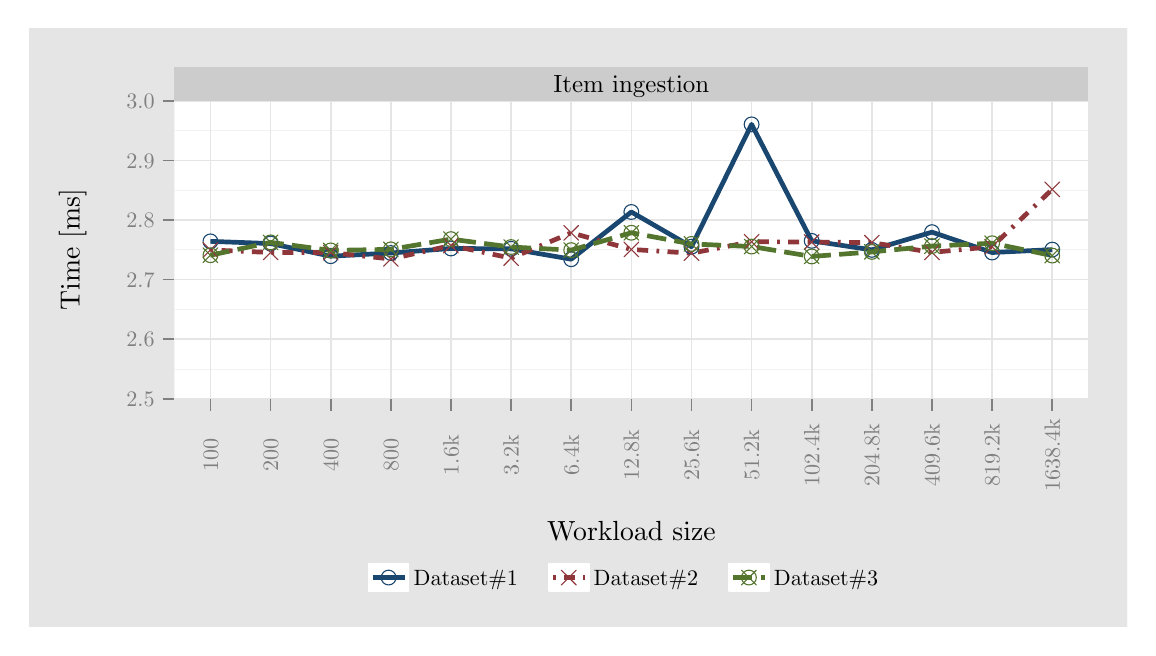
\begin{tikzpicture}[x=1pt,y=1pt]
\definecolor[named]{fillColor}{rgb}{1.00,1.00,1.00}
\path[use as bounding box,fill=fillColor,fill opacity=0.00] (0,0) rectangle (397.48,216.81);
\begin{scope}
\path[clip] (  0.00,  0.00) rectangle (397.48,216.81);
\definecolor[named]{drawColor}{rgb}{1.00,1.00,1.00}
\definecolor[named]{fillColor}{rgb}{0.90,0.90,0.90}

\path[draw=drawColor,line width= 0.6pt,line join=round,line cap=round,fill=fillColor] (  0.00,  0.00) rectangle (397.48,216.81);
\end{scope}
\begin{scope}
\path[clip] ( 53.00, 82.69) rectangle (383.26,190.36);
\definecolor[named]{fillColor}{rgb}{1.00,1.00,1.00}

\path[fill=fillColor] ( 53.00, 82.69) rectangle (383.26,190.36);
\definecolor[named]{drawColor}{rgb}{0.95,0.95,0.95}

\path[draw=drawColor,line width= 0.3pt,line join=round] ( 53.00, 93.46) --
	(383.26, 93.46);

\path[draw=drawColor,line width= 0.3pt,line join=round] ( 53.00,114.99) --
	(383.26,114.99);

\path[draw=drawColor,line width= 0.3pt,line join=round] ( 53.00,136.53) --
	(383.26,136.53);

\path[draw=drawColor,line width= 0.3pt,line join=round] ( 53.00,158.06) --
	(383.26,158.06);

\path[draw=drawColor,line width= 0.3pt,line join=round] ( 53.00,179.60) --
	(383.26,179.60);
\definecolor[named]{drawColor}{rgb}{0.90,0.90,0.90}

\path[draw=drawColor,line width= 0.6pt,line join=round] ( 53.00, 82.69) --
	(383.26, 82.69);

\path[draw=drawColor,line width= 0.6pt,line join=round] ( 53.00,104.23) --
	(383.26,104.23);

\path[draw=drawColor,line width= 0.6pt,line join=round] ( 53.00,125.76) --
	(383.26,125.76);

\path[draw=drawColor,line width= 0.6pt,line join=round] ( 53.00,147.29) --
	(383.26,147.29);

\path[draw=drawColor,line width= 0.6pt,line join=round] ( 53.00,168.83) --
	(383.26,168.83);

\path[draw=drawColor,line width= 0.6pt,line join=round] ( 53.00,190.36) --
	(383.26,190.36);

\path[draw=drawColor,line width= 0.6pt,line join=round] ( 66.04, 82.69) --
	( 66.04,190.36);

\path[draw=drawColor,line width= 0.6pt,line join=round] ( 87.77, 82.69) --
	( 87.77,190.36);

\path[draw=drawColor,line width= 0.6pt,line join=round] (109.50, 82.69) --
	(109.50,190.36);

\path[draw=drawColor,line width= 0.6pt,line join=round] (131.22, 82.69) --
	(131.22,190.36);

\path[draw=drawColor,line width= 0.6pt,line join=round] (152.95, 82.69) --
	(152.95,190.36);

\path[draw=drawColor,line width= 0.6pt,line join=round] (174.68, 82.69) --
	(174.68,190.36);

\path[draw=drawColor,line width= 0.6pt,line join=round] (196.40, 82.69) --
	(196.40,190.36);

\path[draw=drawColor,line width= 0.6pt,line join=round] (218.13, 82.69) --
	(218.13,190.36);

\path[draw=drawColor,line width= 0.6pt,line join=round] (239.86, 82.69) --
	(239.86,190.36);

\path[draw=drawColor,line width= 0.6pt,line join=round] (261.59, 82.69) --
	(261.59,190.36);

\path[draw=drawColor,line width= 0.6pt,line join=round] (283.31, 82.69) --
	(283.31,190.36);

\path[draw=drawColor,line width= 0.6pt,line join=round] (305.04, 82.69) --
	(305.04,190.36);

\path[draw=drawColor,line width= 0.6pt,line join=round] (326.77, 82.69) --
	(326.77,190.36);

\path[draw=drawColor,line width= 0.6pt,line join=round] (348.50, 82.69) --
	(348.50,190.36);

\path[draw=drawColor,line width= 0.6pt,line join=round] (370.22, 82.69) --
	(370.22,190.36);
\definecolor[named]{drawColor}{rgb}{0.10,0.28,0.44}

\path[draw=drawColor,line width= 1.7pt,line join=round] ( 66.04,139.59) --
	( 87.77,138.80) --
	(109.50,134.23) --
	(131.22,135.39) --
	(152.95,137.02) --
	(174.68,136.91) --
	(196.40,133.14) --
	(218.13,150.21) --
	(239.86,137.65) --
	(261.59,181.86) --
	(283.31,139.77) --
	(305.04,136.51) --
	(326.77,142.92) --
	(348.50,135.56) --
	(370.22,136.61);
\definecolor[named]{drawColor}{rgb}{0.56,0.21,0.23}

\path[draw=drawColor,line width= 1.7pt,dash pattern=on 1pt off 3pt on 4pt off 3pt ,line join=round] ( 66.04,136.47) --
	( 87.77,135.58) --
	(109.50,135.53) --
	(131.22,133.23) --
	(152.95,138.09) --
	(174.68,133.53) --
	(196.40,142.68) --
	(218.13,136.67) --
	(239.86,135.32) --
	(261.59,139.45) --
	(283.31,139.35) --
	(305.04,139.14) --
	(326.77,135.60) --
	(348.50,137.67) --
	(370.22,158.40);
\definecolor[named]{drawColor}{rgb}{0.33,0.46,0.18}

\path[draw=drawColor,line width= 1.7pt,dash pattern=on 7pt off 3pt ,line join=round] ( 66.04,134.58) --
	( 87.77,139.23) --
	(109.50,136.32) --
	(131.22,136.70) --
	(152.95,140.40) --
	(174.68,137.54) --
	(196.40,136.42) --
	(218.13,142.70) --
	(239.86,138.66) --
	(261.59,137.72) --
	(283.31,134.14) --
	(305.04,135.79) --
	(326.77,137.88) --
	(348.50,138.91) --
	(370.22,134.46);
\definecolor[named]{drawColor}{rgb}{0.10,0.28,0.44}

\path[draw=drawColor,line width= 0.4pt,line join=round,line cap=round] ( 66.04,139.59) circle (  2.67);

\path[draw=drawColor,line width= 0.4pt,line join=round,line cap=round] ( 87.77,138.80) circle (  2.67);

\path[draw=drawColor,line width= 0.4pt,line join=round,line cap=round] (109.50,134.23) circle (  2.67);

\path[draw=drawColor,line width= 0.4pt,line join=round,line cap=round] (131.22,135.39) circle (  2.67);

\path[draw=drawColor,line width= 0.4pt,line join=round,line cap=round] (152.95,137.02) circle (  2.67);

\path[draw=drawColor,line width= 0.4pt,line join=round,line cap=round] (174.68,136.91) circle (  2.67);

\path[draw=drawColor,line width= 0.4pt,line join=round,line cap=round] (196.40,133.14) circle (  2.67);

\path[draw=drawColor,line width= 0.4pt,line join=round,line cap=round] (218.13,150.21) circle (  2.67);

\path[draw=drawColor,line width= 0.4pt,line join=round,line cap=round] (239.86,137.65) circle (  2.67);

\path[draw=drawColor,line width= 0.4pt,line join=round,line cap=round] (261.59,181.86) circle (  2.67);

\path[draw=drawColor,line width= 0.4pt,line join=round,line cap=round] (283.31,139.77) circle (  2.67);

\path[draw=drawColor,line width= 0.4pt,line join=round,line cap=round] (305.04,136.51) circle (  2.67);

\path[draw=drawColor,line width= 0.4pt,line join=round,line cap=round] (326.77,142.92) circle (  2.67);

\path[draw=drawColor,line width= 0.4pt,line join=round,line cap=round] (348.50,135.56) circle (  2.67);

\path[draw=drawColor,line width= 0.4pt,line join=round,line cap=round] (370.22,136.61) circle (  2.67);
\definecolor[named]{drawColor}{rgb}{0.56,0.21,0.23}

\path[draw=drawColor,line width= 0.4pt,line join=round,line cap=round,fill=fillColor] ( 63.37,133.81) -- ( 68.71,139.14);

\path[draw=drawColor,line width= 0.4pt,line join=round,line cap=round,fill=fillColor] ( 63.37,139.14) -- ( 68.71,133.81);

\path[draw=drawColor,line width= 0.4pt,line join=round,line cap=round,fill=fillColor] ( 85.10,132.91) -- ( 90.44,138.25);

\path[draw=drawColor,line width= 0.4pt,line join=round,line cap=round,fill=fillColor] ( 85.10,138.25) -- ( 90.44,132.91);

\path[draw=drawColor,line width= 0.4pt,line join=round,line cap=round,fill=fillColor] (106.83,132.86) -- (112.16,138.20);

\path[draw=drawColor,line width= 0.4pt,line join=round,line cap=round,fill=fillColor] (106.83,138.20) -- (112.16,132.86);

\path[draw=drawColor,line width= 0.4pt,line join=round,line cap=round,fill=fillColor] (128.56,130.56) -- (133.89,135.90);

\path[draw=drawColor,line width= 0.4pt,line join=round,line cap=round,fill=fillColor] (128.56,135.90) -- (133.89,130.56);

\path[draw=drawColor,line width= 0.4pt,line join=round,line cap=round,fill=fillColor] (150.28,135.42) -- (155.62,140.75);

\path[draw=drawColor,line width= 0.4pt,line join=round,line cap=round,fill=fillColor] (150.28,140.75) -- (155.62,135.42);

\path[draw=drawColor,line width= 0.4pt,line join=round,line cap=round,fill=fillColor] (172.01,130.86) -- (177.34,136.20);

\path[draw=drawColor,line width= 0.4pt,line join=round,line cap=round,fill=fillColor] (172.01,136.20) -- (177.34,130.86);

\path[draw=drawColor,line width= 0.4pt,line join=round,line cap=round,fill=fillColor] (193.74,140.01) -- (199.07,145.35);

\path[draw=drawColor,line width= 0.4pt,line join=round,line cap=round,fill=fillColor] (193.74,145.35) -- (199.07,140.01);

\path[draw=drawColor,line width= 0.4pt,line join=round,line cap=round,fill=fillColor] (215.46,134.00) -- (220.80,139.33);

\path[draw=drawColor,line width= 0.4pt,line join=round,line cap=round,fill=fillColor] (215.46,139.33) -- (220.80,134.00);

\path[draw=drawColor,line width= 0.4pt,line join=round,line cap=round,fill=fillColor] (237.19,132.65) -- (242.53,137.98);

\path[draw=drawColor,line width= 0.4pt,line join=round,line cap=round,fill=fillColor] (237.19,137.98) -- (242.53,132.65);

\path[draw=drawColor,line width= 0.4pt,line join=round,line cap=round,fill=fillColor] (258.92,136.79) -- (264.25,142.12);

\path[draw=drawColor,line width= 0.4pt,line join=round,line cap=round,fill=fillColor] (258.92,142.12) -- (264.25,136.79);

\path[draw=drawColor,line width= 0.4pt,line join=round,line cap=round,fill=fillColor] (280.65,136.68) -- (285.98,142.02);

\path[draw=drawColor,line width= 0.4pt,line join=round,line cap=round,fill=fillColor] (280.65,142.02) -- (285.98,136.68);

\path[draw=drawColor,line width= 0.4pt,line join=round,line cap=round,fill=fillColor] (302.37,136.47) -- (307.71,141.81);

\path[draw=drawColor,line width= 0.4pt,line join=round,line cap=round,fill=fillColor] (302.37,141.81) -- (307.71,136.47);

\path[draw=drawColor,line width= 0.4pt,line join=round,line cap=round,fill=fillColor] (324.10,132.93) -- (329.44,138.27);

\path[draw=drawColor,line width= 0.4pt,line join=round,line cap=round,fill=fillColor] (324.10,138.27) -- (329.44,132.93);

\path[draw=drawColor,line width= 0.4pt,line join=round,line cap=round,fill=fillColor] (345.83,135.00) -- (351.16,140.33);

\path[draw=drawColor,line width= 0.4pt,line join=round,line cap=round,fill=fillColor] (345.83,140.33) -- (351.16,135.00);

\path[draw=drawColor,line width= 0.4pt,line join=round,line cap=round,fill=fillColor] (367.55,155.73) -- (372.89,161.07);

\path[draw=drawColor,line width= 0.4pt,line join=round,line cap=round,fill=fillColor] (367.55,161.07) -- (372.89,155.73);
\definecolor[named]{drawColor}{rgb}{0.33,0.46,0.18}

\path[draw=drawColor,line width= 0.4pt,line join=round,line cap=round] ( 66.04,134.58) circle (  2.67);

\path[draw=drawColor,line width= 0.4pt,line join=round,line cap=round] ( 63.37,131.91) -- ( 68.71,137.25);

\path[draw=drawColor,line width= 0.4pt,line join=round,line cap=round] ( 63.37,137.25) -- ( 68.71,131.91);

\path[draw=drawColor,line width= 0.4pt,line join=round,line cap=round] ( 87.77,139.23) circle (  2.67);

\path[draw=drawColor,line width= 0.4pt,line join=round,line cap=round] ( 85.10,136.56) -- ( 90.44,141.89);

\path[draw=drawColor,line width= 0.4pt,line join=round,line cap=round] ( 85.10,141.89) -- ( 90.44,136.56);

\path[draw=drawColor,line width= 0.4pt,line join=round,line cap=round] (109.50,136.32) circle (  2.67);

\path[draw=drawColor,line width= 0.4pt,line join=round,line cap=round] (106.83,133.65) -- (112.16,138.98);

\path[draw=drawColor,line width= 0.4pt,line join=round,line cap=round] (106.83,138.98) -- (112.16,133.65);

\path[draw=drawColor,line width= 0.4pt,line join=round,line cap=round] (131.22,136.70) circle (  2.67);

\path[draw=drawColor,line width= 0.4pt,line join=round,line cap=round] (128.56,134.03) -- (133.89,139.37);

\path[draw=drawColor,line width= 0.4pt,line join=round,line cap=round] (128.56,139.37) -- (133.89,134.03);

\path[draw=drawColor,line width= 0.4pt,line join=round,line cap=round] (152.95,140.40) circle (  2.67);

\path[draw=drawColor,line width= 0.4pt,line join=round,line cap=round] (150.28,137.73) -- (155.62,143.07);

\path[draw=drawColor,line width= 0.4pt,line join=round,line cap=round] (150.28,143.07) -- (155.62,137.73);

\path[draw=drawColor,line width= 0.4pt,line join=round,line cap=round] (174.68,137.54) circle (  2.67);

\path[draw=drawColor,line width= 0.4pt,line join=round,line cap=round] (172.01,134.88) -- (177.34,140.21);

\path[draw=drawColor,line width= 0.4pt,line join=round,line cap=round] (172.01,140.21) -- (177.34,134.88);

\path[draw=drawColor,line width= 0.4pt,line join=round,line cap=round] (196.40,136.42) circle (  2.67);

\path[draw=drawColor,line width= 0.4pt,line join=round,line cap=round] (193.74,133.75) -- (199.07,139.09);

\path[draw=drawColor,line width= 0.4pt,line join=round,line cap=round] (193.74,139.09) -- (199.07,133.75);

\path[draw=drawColor,line width= 0.4pt,line join=round,line cap=round] (218.13,142.70) circle (  2.67);

\path[draw=drawColor,line width= 0.4pt,line join=round,line cap=round] (215.46,140.03) -- (220.80,145.36);

\path[draw=drawColor,line width= 0.4pt,line join=round,line cap=round] (215.46,145.36) -- (220.80,140.03);

\path[draw=drawColor,line width= 0.4pt,line join=round,line cap=round] (239.86,138.66) circle (  2.67);

\path[draw=drawColor,line width= 0.4pt,line join=round,line cap=round] (237.19,136.00) -- (242.53,141.33);

\path[draw=drawColor,line width= 0.4pt,line join=round,line cap=round] (237.19,141.33) -- (242.53,136.00);

\path[draw=drawColor,line width= 0.4pt,line join=round,line cap=round] (261.59,137.72) circle (  2.67);

\path[draw=drawColor,line width= 0.4pt,line join=round,line cap=round] (258.92,135.05) -- (264.25,140.39);

\path[draw=drawColor,line width= 0.4pt,line join=round,line cap=round] (258.92,140.39) -- (264.25,135.05);

\path[draw=drawColor,line width= 0.4pt,line join=round,line cap=round] (283.31,134.14) circle (  2.67);

\path[draw=drawColor,line width= 0.4pt,line join=round,line cap=round] (280.65,131.48) -- (285.98,136.81);

\path[draw=drawColor,line width= 0.4pt,line join=round,line cap=round] (280.65,136.81) -- (285.98,131.48);

\path[draw=drawColor,line width= 0.4pt,line join=round,line cap=round] (305.04,135.79) circle (  2.67);

\path[draw=drawColor,line width= 0.4pt,line join=round,line cap=round] (302.37,133.12) -- (307.71,138.46);

\path[draw=drawColor,line width= 0.4pt,line join=round,line cap=round] (302.37,138.46) -- (307.71,133.12);

\path[draw=drawColor,line width= 0.4pt,line join=round,line cap=round] (326.77,137.88) circle (  2.67);

\path[draw=drawColor,line width= 0.4pt,line join=round,line cap=round] (324.10,135.21) -- (329.44,140.54);

\path[draw=drawColor,line width= 0.4pt,line join=round,line cap=round] (324.10,140.54) -- (329.44,135.21);

\path[draw=drawColor,line width= 0.4pt,line join=round,line cap=round] (348.50,138.91) circle (  2.67);

\path[draw=drawColor,line width= 0.4pt,line join=round,line cap=round] (345.83,136.24) -- (351.16,141.58);

\path[draw=drawColor,line width= 0.4pt,line join=round,line cap=round] (345.83,141.58) -- (351.16,136.24);

\path[draw=drawColor,line width= 0.4pt,line join=round,line cap=round] (370.22,134.46) circle (  2.67);

\path[draw=drawColor,line width= 0.4pt,line join=round,line cap=round] (367.55,131.79) -- (372.89,137.13);

\path[draw=drawColor,line width= 0.4pt,line join=round,line cap=round] (367.55,137.13) -- (372.89,131.79);
\end{scope}
\begin{scope}
\path[clip] (  0.00,  0.00) rectangle (397.48,216.81);
\definecolor[named]{fillColor}{rgb}{0.80,0.80,0.80}

\path[fill=fillColor] ( 53.00,190.36) rectangle (383.26,202.58);
\definecolor[named]{drawColor}{rgb}{0.00,0.00,0.00}

\node[text=drawColor,anchor=base,inner sep=0pt, outer sep=0pt, scale=  0.90] at (218.13,193.37) {Item ingestion};
\end{scope}
\begin{scope}
\path[clip] (  0.00,  0.00) rectangle (397.48,216.81);
\definecolor[named]{drawColor}{rgb}{0.50,0.50,0.50}

\node[text=drawColor,anchor=base east,inner sep=0pt, outer sep=0pt, scale=  0.80] at ( 45.89, 79.94) {2.5};

\node[text=drawColor,anchor=base east,inner sep=0pt, outer sep=0pt, scale=  0.80] at ( 45.89,101.47) {2.6};

\node[text=drawColor,anchor=base east,inner sep=0pt, outer sep=0pt, scale=  0.80] at ( 45.89,123.00) {2.7};

\node[text=drawColor,anchor=base east,inner sep=0pt, outer sep=0pt, scale=  0.80] at ( 45.89,144.54) {2.8};

\node[text=drawColor,anchor=base east,inner sep=0pt, outer sep=0pt, scale=  0.80] at ( 45.89,166.07) {2.9};

\node[text=drawColor,anchor=base east,inner sep=0pt, outer sep=0pt, scale=  0.80] at ( 45.89,187.61) {3.0};
\end{scope}
\begin{scope}
\path[clip] (  0.00,  0.00) rectangle (397.48,216.81);
\definecolor[named]{drawColor}{rgb}{0.50,0.50,0.50}

\path[draw=drawColor,line width= 0.6pt,line join=round] ( 48.74, 82.69) --
	( 53.00, 82.69);

\path[draw=drawColor,line width= 0.6pt,line join=round] ( 48.74,104.23) --
	( 53.00,104.23);

\path[draw=drawColor,line width= 0.6pt,line join=round] ( 48.74,125.76) --
	( 53.00,125.76);

\path[draw=drawColor,line width= 0.6pt,line join=round] ( 48.74,147.29) --
	( 53.00,147.29);

\path[draw=drawColor,line width= 0.6pt,line join=round] ( 48.74,168.83) --
	( 53.00,168.83);

\path[draw=drawColor,line width= 0.6pt,line join=round] ( 48.74,190.36) --
	( 53.00,190.36);
\end{scope}
\begin{scope}
\path[clip] (  0.00,  0.00) rectangle (397.48,216.81);
\definecolor[named]{drawColor}{rgb}{0.50,0.50,0.50}

\path[draw=drawColor,line width= 0.6pt,line join=round] ( 66.04, 78.42) --
	( 66.04, 82.69);

\path[draw=drawColor,line width= 0.6pt,line join=round] ( 87.77, 78.42) --
	( 87.77, 82.69);

\path[draw=drawColor,line width= 0.6pt,line join=round] (109.50, 78.42) --
	(109.50, 82.69);

\path[draw=drawColor,line width= 0.6pt,line join=round] (131.22, 78.42) --
	(131.22, 82.69);

\path[draw=drawColor,line width= 0.6pt,line join=round] (152.95, 78.42) --
	(152.95, 82.69);

\path[draw=drawColor,line width= 0.6pt,line join=round] (174.68, 78.42) --
	(174.68, 82.69);

\path[draw=drawColor,line width= 0.6pt,line join=round] (196.40, 78.42) --
	(196.40, 82.69);

\path[draw=drawColor,line width= 0.6pt,line join=round] (218.13, 78.42) --
	(218.13, 82.69);

\path[draw=drawColor,line width= 0.6pt,line join=round] (239.86, 78.42) --
	(239.86, 82.69);

\path[draw=drawColor,line width= 0.6pt,line join=round] (261.59, 78.42) --
	(261.59, 82.69);

\path[draw=drawColor,line width= 0.6pt,line join=round] (283.31, 78.42) --
	(283.31, 82.69);

\path[draw=drawColor,line width= 0.6pt,line join=round] (305.04, 78.42) --
	(305.04, 82.69);

\path[draw=drawColor,line width= 0.6pt,line join=round] (326.77, 78.42) --
	(326.77, 82.69);

\path[draw=drawColor,line width= 0.6pt,line join=round] (348.50, 78.42) --
	(348.50, 82.69);

\path[draw=drawColor,line width= 0.6pt,line join=round] (370.22, 78.42) --
	(370.22, 82.69);
\end{scope}
\begin{scope}
\path[clip] (  0.00,  0.00) rectangle (397.48,216.81);
\definecolor[named]{drawColor}{rgb}{0.50,0.50,0.50}

\node[text=drawColor,rotate= 90.00,anchor=base,inner sep=0pt, outer sep=0pt, scale=  0.80] at ( 68.80, 62.36) {100};

\node[text=drawColor,rotate= 90.00,anchor=base,inner sep=0pt, outer sep=0pt, scale=  0.80] at ( 90.52, 62.36) {200};

\node[text=drawColor,rotate= 90.00,anchor=base,inner sep=0pt, outer sep=0pt, scale=  0.80] at (112.25, 62.36) {400};

\node[text=drawColor,rotate= 90.00,anchor=base,inner sep=0pt, outer sep=0pt, scale=  0.80] at (133.98, 62.36) {800};

\node[text=drawColor,rotate= 90.00,anchor=base,inner sep=0pt, outer sep=0pt, scale=  0.80] at (155.70, 62.36) {1.6k};

\node[text=drawColor,rotate= 90.00,anchor=base,inner sep=0pt, outer sep=0pt, scale=  0.80] at (177.43, 62.36) {3.2k};

\node[text=drawColor,rotate= 90.00,anchor=base,inner sep=0pt, outer sep=0pt, scale=  0.80] at (199.16, 62.36) {6.4k};

\node[text=drawColor,rotate= 90.00,anchor=base,inner sep=0pt, outer sep=0pt, scale=  0.80] at (220.89, 62.36) {12.8k};

\node[text=drawColor,rotate= 90.00,anchor=base,inner sep=0pt, outer sep=0pt, scale=  0.80] at (242.61, 62.36) {25.6k};

\node[text=drawColor,rotate= 90.00,anchor=base,inner sep=0pt, outer sep=0pt, scale=  0.80] at (264.34, 62.36) {51.2k};

\node[text=drawColor,rotate= 90.00,anchor=base,inner sep=0pt, outer sep=0pt, scale=  0.80] at (286.07, 62.36) {102.4k};

\node[text=drawColor,rotate= 90.00,anchor=base,inner sep=0pt, outer sep=0pt, scale=  0.80] at (307.80, 62.36) {204.8k};

\node[text=drawColor,rotate= 90.00,anchor=base,inner sep=0pt, outer sep=0pt, scale=  0.80] at (329.52, 62.36) {409.6k};

\node[text=drawColor,rotate= 90.00,anchor=base,inner sep=0pt, outer sep=0pt, scale=  0.80] at (351.25, 62.36) {819.2k};

\node[text=drawColor,rotate= 90.00,anchor=base,inner sep=0pt, outer sep=0pt, scale=  0.80] at (372.98, 62.36) {1638.4k};
\end{scope}
\begin{scope}
\path[clip] (  0.00,  0.00) rectangle (397.48,216.81);
\definecolor[named]{drawColor}{rgb}{0.00,0.00,0.00}

\node[text=drawColor,anchor=base,inner sep=0pt, outer sep=0pt, scale=  1.00] at (218.13, 31.41) {Workload size};
\end{scope}
\begin{scope}
\path[clip] (  0.00,  0.00) rectangle (397.48,216.81);
\definecolor[named]{drawColor}{rgb}{0.00,0.00,0.00}

\node[text=drawColor,rotate= 90.00,anchor=base,inner sep=0pt, outer sep=0pt, scale=  1.00] at ( 18.80,136.53) {Time [ms]};
\end{scope}
\begin{scope}
\path[clip] (  0.00,  0.00) rectangle (397.48,216.81);
\definecolor[named]{fillColor}{rgb}{0.90,0.90,0.90}

\path[fill=fillColor] (115.31,  8.87) rectangle (320.96, 27.36);
\end{scope}
\begin{scope}
\path[clip] (  0.00,  0.00) rectangle (397.48,216.81);
\definecolor[named]{drawColor}{rgb}{1.00,1.00,1.00}
\definecolor[named]{fillColor}{rgb}{1.00,1.00,1.00}

\path[draw=drawColor,line width= 0.6pt,line join=round,line cap=round,fill=fillColor] (123.19, 13.14) rectangle (137.64, 23.09);
\end{scope}
\begin{scope}
\path[clip] (  0.00,  0.00) rectangle (397.48,216.81);
\definecolor[named]{drawColor}{rgb}{0.10,0.28,0.44}

\path[draw=drawColor,line width= 1.7pt,line join=round] (124.63, 18.11) -- (136.20, 18.11);
\end{scope}
\begin{scope}
\path[clip] (  0.00,  0.00) rectangle (397.48,216.81);
\definecolor[named]{drawColor}{rgb}{0.10,0.28,0.44}

\path[draw=drawColor,line width= 0.4pt,line join=round,line cap=round] (130.42, 18.11) circle (  2.67);
\end{scope}
\begin{scope}
\path[clip] (  0.00,  0.00) rectangle (397.48,216.81);
\definecolor[named]{drawColor}{rgb}{1.00,1.00,1.00}
\definecolor[named]{fillColor}{rgb}{1.00,1.00,1.00}

\path[draw=drawColor,line width= 0.6pt,line join=round,line cap=round,fill=fillColor] (188.29, 13.14) rectangle (202.74, 23.09);
\end{scope}
\begin{scope}
\path[clip] (  0.00,  0.00) rectangle (397.48,216.81);
\definecolor[named]{drawColor}{rgb}{0.56,0.21,0.23}

\path[draw=drawColor,line width= 1.7pt,dash pattern=on 1pt off 3pt on 4pt off 3pt ,line join=round] (189.74, 18.11) -- (201.30, 18.11);
\end{scope}
\begin{scope}
\path[clip] (  0.00,  0.00) rectangle (397.48,216.81);
\definecolor[named]{drawColor}{rgb}{0.56,0.21,0.23}
\definecolor[named]{fillColor}{rgb}{1.00,1.00,1.00}

\path[draw=drawColor,line width= 0.4pt,line join=round,line cap=round,fill=fillColor] (192.85, 15.45) -- (198.19, 20.78);

\path[draw=drawColor,line width= 0.4pt,line join=round,line cap=round,fill=fillColor] (192.85, 20.78) -- (198.19, 15.45);
\end{scope}
\begin{scope}
\path[clip] (  0.00,  0.00) rectangle (397.48,216.81);
\definecolor[named]{drawColor}{rgb}{1.00,1.00,1.00}
\definecolor[named]{fillColor}{rgb}{1.00,1.00,1.00}

\path[draw=drawColor,line width= 0.6pt,line join=round,line cap=round,fill=fillColor] (253.39, 13.14) rectangle (267.85, 23.09);
\end{scope}
\begin{scope}
\path[clip] (  0.00,  0.00) rectangle (397.48,216.81);
\definecolor[named]{drawColor}{rgb}{0.33,0.46,0.18}

\path[draw=drawColor,line width= 1.7pt,dash pattern=on 7pt off 3pt ,line join=round] (254.84, 18.11) -- (266.40, 18.11);
\end{scope}
\begin{scope}
\path[clip] (  0.00,  0.00) rectangle (397.48,216.81);
\definecolor[named]{drawColor}{rgb}{0.33,0.46,0.18}

\path[draw=drawColor,line width= 0.4pt,line join=round,line cap=round] (260.62, 18.11) circle (  2.67);

\path[draw=drawColor,line width= 0.4pt,line join=round,line cap=round] (257.95, 15.45) -- (263.29, 20.78);

\path[draw=drawColor,line width= 0.4pt,line join=round,line cap=round] (257.95, 20.78) -- (263.29, 15.45);
\end{scope}
\begin{scope}
\path[clip] (  0.00,  0.00) rectangle (397.48,216.81);
\definecolor[named]{drawColor}{rgb}{0.00,0.00,0.00}

\node[text=drawColor,anchor=base west,inner sep=0pt, outer sep=0pt, scale=  0.80] at (139.45, 15.36) {Dataset\#1 $\;\;\;$};
\end{scope}
\begin{scope}
\path[clip] (  0.00,  0.00) rectangle (397.48,216.81);
\definecolor[named]{drawColor}{rgb}{0.00,0.00,0.00}

\node[text=drawColor,anchor=base west,inner sep=0pt, outer sep=0pt, scale=  0.80] at (204.55, 15.36) {Dataset\#2 $\;\;\;$};
\end{scope}
\begin{scope}
\path[clip] (  0.00,  0.00) rectangle (397.48,216.81);
\definecolor[named]{drawColor}{rgb}{0.00,0.00,0.00}

\node[text=drawColor,anchor=base west,inner sep=0pt, outer sep=0pt, scale=  0.80] at (269.65, 15.36) {Dataset\#3 $\;\;\;$};
\end{scope}
\end{tikzpicture}

 }
 \caption[Impact of structure on item ingestion\index{Ingestion} performance]{The average time, in milliseconds, taken to ingest a single item into an existing collection.}
 \label{fig:experimentation:performance:ingest:plot.experimentation.performance.ingest.single-item}
\end{figure}

%%\subsubsection{Discussion}
%%\label{sec:evaluation:performance:ingestion:discussion}
\subparagraph{Discussion}

The ingestion\index{Ingestion} response times remain constant irrespective of the workload\index{Workload} size. This is because the only overhead incurred results from disk write IO. It should be noted that this experiment mimicked an ideal situation where the destination location for the item is known before hand.

%%\subsubsection{Conclusion}
%%\label{sec:evaluation:performance:ingestion:conclusion}

The workload\index{Workload} size does not affect the ingestion\index{Ingestion} response time.

\subsubsection{Full-text search}
\label{sec:evaluation:performance:search-and-browse}

The purpose of these experiments was to determine the impact on collection size on
query performance for indexed and non-indexed collections.

\paragraph{Experiment: Search performance for unindexed collections}
\label{sec:evaluation:performance:search-browse:experiment1}

This experiment was conducted to determine query performance of non-indexed collections.

\subparagraph{Methodology}

The most frequently occurring terms in the workloads were identified and search\index{Search} requests issued to determine response times. The search\index{Search} module implementation involved traversing collection containers and successively parsing\index{Parsing} and querying each metadata\index{Metadata} file in the collection for the search\index{Search} phrase in question.

\subparagraph{Results}

The mean response times taken to generate search\index{Search} query resultsets are shown in Figure~\ref{fig:experimentation:performance:search:processing-phases-cumulative}. In order to ascertain the overall distribution of the search\index{Search} response times, the time taken for the various search\index{Search} phases---directory traversal, parsing\index{Parsing} and XPath\index{XPath} querying---was noted; Table~\ref{tab:experimentation:performance:search:processing-phases-benchmark} and Figure~\ref{fig:experimentation:performance:search:processing-phases-cumulative} show these times for the \num{15} workloads.\index{Workload}

\tablespacing
%\begin{longtable}{p{0.12\linewidth} p{0.12\linewidth} p{0.12\linewidth}
%p{0.12\linewidth} p{0.12\linewidth} p{0.12\linewidth} p{0.12\linewidth}}
\begin{longtable}{
>{\arraybackslash}m{0.07\linewidth}|
>{\centering\arraybackslash}m{0.18\linewidth}|
>{\centering\arraybackslash}m{0.12\linewidth}| 
>{\centering\arraybackslash}m{0.10\linewidth}|
>{\centering\arraybackslash}m{0.10\linewidth}}

\caption{Baseline performance benchmarks for full-text search}
\label{tab:experimentation:performance:search:processing-phases-benchmark}\\

 %%%%%\toprule
 \hline
 {} & 
{\textbf{Time [ms]}}&
{\textbf{Traversal}}&
{\textbf{Parsing}}&
{\textbf{XPath}} \\
%%%%%\midrule
\hline \hline
 \endfirsthead

 \caption[]{(continued)}\\
 %%%%%\toprule
 \hline
 {} & 
{\textbf{Time [ms]}}&
{\textbf{Traversal}}&
{\textbf{Parsing}}&
{\textbf{XPath}} \\
%%%%%\midrule
\hline \hline
 \endhead

 % Page footer
 %%%%\midrule
 \hline
 \multicolumn{5}{r}{(Continued on next page)} \\
 \endfoot

 % Last page footer
 \bottomrule
 \endlastfoot

%%\textbf{W1} & {\SI{16.13}{\percent}} & {\SI{38.49}{\percent}} & {\SI{45.38}{\percent}} \\ 
%%\textbf{W2} & {\SI{15.40}{\percent}} & {\SI{39.05}{\percent}} & {\SI{45.54}{\percent}} \\ 
%%\textbf{W3} & {\SI{14.89}{\percent}} & {\SI{39.01}{\percent}} & {\SI{46.10}{\percent}} \\ 
%%\textbf{W4} & {\SI{14.28}{\percent}} & {\SI{39.45}{\percent}} & {\SI{46.27}{\percent}} \\ 
%%\textbf{W5} & {\SI{13.82}{\percent}} & {\SI{39.39}{\percent}} & {\SI{46.79}{\percent}} \\ 
%%\textbf{W6} & {\SI{13.58}{\percent}} & {\SI{39.58}{\percent}} & {\SI{46.84}{\percent}} \\ 
%%\textbf{W7} & {\SI{13.55}{\percent}} & {\SI{39.37}{\percent}} & {\SI{47.08}{\percent}} \\ 
%%\textbf{W8} & {\SI{13.41}{\percent}} & {\SI{39.52}{\percent}} & {\SI{47.08}{\percent}} \\ 
%%\textbf{W9} & {\SI{13.37}{\percent}} & {\SI{39.76}{\percent}} & {\SI{46.87}{\percent}} \\ 
%%\textbf{W10} & {\SI{13.66}{\percent}} & {\SI{39.72}{\percent}} & {\SI{46.63}{\percent}} \\ 
%%\textbf{W11} & {\SI{14.20}{\percent}} & {\SI{39.49}{\percent}} & {\SI{46.31}{\percent}} \\ 
%%\textbf{W12} & {\SI{13.51}{\percent}} & {\SI{39.65}{\percent}} & {\SI{46.85}{\percent}} \\ 
%%\textbf{W13} & {\SI{14.20}{\percent}} & {\SI{39.85}{\percent}} & {\SI{45.95}{\percent}} \\ 
%%\textbf{W14} & {\SI{1.99}{\percent}} & {\SI{95.57}{\percent}} & {\SI{2.44}{\percent}} \\ 
%%\textbf{W15} & {\SI{5.28}{\percent}} & {\SI{92.87}{\percent}} & {\SI{1.85}{\percent}} \\ 

\textbf{W1} & {\tablenum[table-format=6.2]{24.67}} & {\SI{16.13}{\percent}} & {\SI{38.49}{\percent}} & {\SI{45.38}{\percent}} \\ 
\textbf{W2} & {\tablenum[table-format=6.2]{47.87}} & {\SI{15.40}{\percent}} & {\SI{39.05}{\percent}} & {\SI{45.54}{\percent}} \\ 
\textbf{W3} & {\tablenum[table-format=6.2]{97.38}} & {\SI{14.89}{\percent}} & {\SI{39.01}{\percent}} & {\SI{46.10}{\percent}} \\ 
\textbf{W4} & {\tablenum[table-format=6.2]{191.90}} & {\SI{14.28}{\percent}} & {\SI{39.45}{\percent}} & {\SI{46.27}{\percent}} \\ 
\textbf{W5} & {\tablenum[table-format=6.2]{386.99}} & {\SI{13.82}{\percent}} & {\SI{39.39}{\percent}} & {\SI{46.79}{\percent}} \\ 
\textbf{W6} & {\tablenum[table-format=6.2]{768.35}} & {\SI{13.58}{\percent}} & {\SI{39.58}{\percent}} & {\SI{46.84}{\percent}} \\ 
\textbf{W7} & {\tablenum[table-format=6.2]{1531.06}} & {\SI{13.55}{\percent}} & {\SI{39.37}{\percent}} & {\SI{47.08}{\percent}} \\ 
\textbf{W8} & {\tablenum[table-format=6.2]{3093.12}} & {\SI{13.41}{\percent}} & {\SI{39.52}{\percent}} & {\SI{47.08}{\percent}} \\ 
\textbf{W9} & {\tablenum[table-format=6.2]{6172.22}} & {\SI{13.37}{\percent}} & {\SI{39.76}{\percent}} & {\SI{46.87}{\percent}} \\ 
\textbf{W10} & {\tablenum[table-format=6.2]{12487.06}} & {\SI{13.66}{\percent}} & {\SI{39.72}{\percent}} & {\SI{46.63}{\percent}} \\ 
\textbf{W11} & {\tablenum[table-format=6.2]{25108.74}} & {\SI{14.20}{\percent}} & {\SI{39.49}{\percent}} & {\SI{46.31}{\percent}} \\ 
\textbf{W12} & {\tablenum[table-format=6.2]{49301.45}} & {\SI{13.51}{\percent}} & {\SI{39.65}{\percent}} & {\SI{46.85}{\percent}} \\ 
\textbf{W13} & {\tablenum[table-format=6.2]{100267.33}} & {\SI{14.20}{\percent}} & {\SI{39.85}{\percent}} & {\SI{45.95}{\percent}} \\ 
\textbf{W14} & {\tablenum[table-format=6.2]{7365254.00}} & {\SI{1.99}{\percent}} & {\SI{95.57}{\percent}} & {\SI{2.44}{\percent}} \\ 
\textbf{W15} & {\tablenum[table-format=6.2]{18664713.65}} & {\SI{5.28}{\percent}} & {\SI{92.87}{\percent}} & {\SI{1.85}{\percent}} \\ 

 %\cmidrule[0.1pt](l{0.5em}r{0.5em}){1-3}

 \end{longtable}

\bodyspacing

\begin{figure}
 \centering
 \framebox[\textwidth]{%
% Created by tikzDevice version 0.6.2-92-0ad2792 on 2013-03-28 14:53:09
% !TEX encoding = UTF-8 Unicode
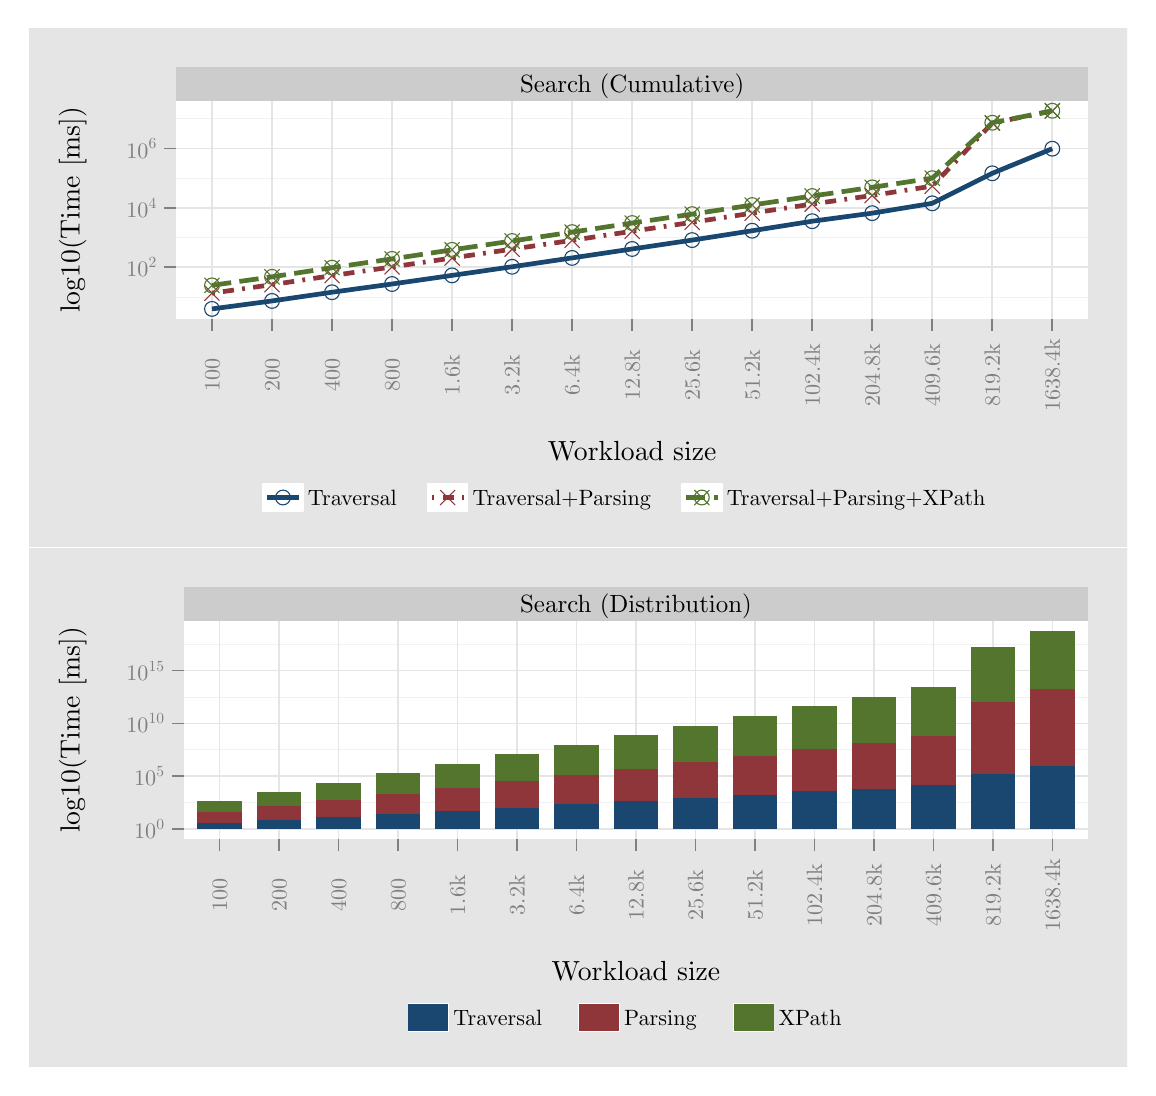
\begin{tikzpicture}[x=1pt,y=1pt]
\definecolor[named]{fillColor}{rgb}{1.00,1.00,1.00}
\path[use as bounding box,fill=fillColor,fill opacity=0.00] (0,0) rectangle (397.48,375.80);
\begin{scope}
\path[clip] (  0.00,187.90) rectangle (397.48,375.80);
\definecolor[named]{drawColor}{rgb}{1.00,1.00,1.00}
\definecolor[named]{fillColor}{rgb}{0.90,0.90,0.90}

\path[draw=drawColor,line width= 0.6pt,line join=round,line cap=round,fill=fillColor] (  0.00,187.90) rectangle (397.48,375.80);
\end{scope}
\begin{scope}
\path[clip] ( 53.58,270.59) rectangle (383.26,349.36);
\definecolor[named]{fillColor}{rgb}{1.00,1.00,1.00}

\path[fill=fillColor] ( 53.58,270.59) rectangle (383.26,349.36);
\definecolor[named]{drawColor}{rgb}{0.95,0.95,0.95}

\path[draw=drawColor,line width= 0.3pt,line join=round] ( 53.58,278.47) --
	(383.26,278.47);

\path[draw=drawColor,line width= 0.3pt,line join=round] ( 53.58,299.93) --
	(383.26,299.93);

\path[draw=drawColor,line width= 0.3pt,line join=round] ( 53.58,321.40) --
	(383.26,321.40);

\path[draw=drawColor,line width= 0.3pt,line join=round] ( 53.58,342.87) --
	(383.26,342.87);
\definecolor[named]{drawColor}{rgb}{0.90,0.90,0.90}

\path[draw=drawColor,line width= 0.6pt,line join=round] ( 53.58,289.20) --
	(383.26,289.20);

\path[draw=drawColor,line width= 0.6pt,line join=round] ( 53.58,310.67) --
	(383.26,310.67);

\path[draw=drawColor,line width= 0.6pt,line join=round] ( 53.58,332.13) --
	(383.26,332.13);

\path[draw=drawColor,line width= 0.6pt,line join=round] ( 66.60,270.59) --
	( 66.60,349.36);

\path[draw=drawColor,line width= 0.6pt,line join=round] ( 88.29,270.59) --
	( 88.29,349.36);

\path[draw=drawColor,line width= 0.6pt,line join=round] (109.97,270.59) --
	(109.97,349.36);

\path[draw=drawColor,line width= 0.6pt,line join=round] (131.66,270.59) --
	(131.66,349.36);

\path[draw=drawColor,line width= 0.6pt,line join=round] (153.35,270.59) --
	(153.35,349.36);

\path[draw=drawColor,line width= 0.6pt,line join=round] (175.04,270.59) --
	(175.04,349.36);

\path[draw=drawColor,line width= 0.6pt,line join=round] (196.73,270.59) --
	(196.73,349.36);

\path[draw=drawColor,line width= 0.6pt,line join=round] (218.42,270.59) --
	(218.42,349.36);

\path[draw=drawColor,line width= 0.6pt,line join=round] (240.11,270.59) --
	(240.11,349.36);

\path[draw=drawColor,line width= 0.6pt,line join=round] (261.80,270.59) --
	(261.80,349.36);

\path[draw=drawColor,line width= 0.6pt,line join=round] (283.49,270.59) --
	(283.49,349.36);

\path[draw=drawColor,line width= 0.6pt,line join=round] (305.18,270.59) --
	(305.18,349.36);

\path[draw=drawColor,line width= 0.6pt,line join=round] (326.87,270.59) --
	(326.87,349.36);

\path[draw=drawColor,line width= 0.6pt,line join=round] (348.56,270.59) --
	(348.56,349.36);

\path[draw=drawColor,line width= 0.6pt,line join=round] (370.25,270.59) --
	(370.25,349.36);
\definecolor[named]{drawColor}{rgb}{0.10,0.28,0.44}

\path[draw=drawColor,line width= 1.7pt,line join=round] ( 66.60,274.17) --
	( 88.29,277.05) --
	(109.97,280.20) --
	(131.66,283.17) --
	(153.35,286.28) --
	(175.04,289.40) --
	(196.73,292.60) --
	(218.42,295.83) --
	(240.11,299.04) --
	(261.80,302.42) --
	(283.49,305.86) --
	(305.18,308.77) --
	(326.87,312.32) --
	(348.56,323.17) --
	(370.25,332.06);
\definecolor[named]{drawColor}{rgb}{0.56,0.21,0.23}

\path[draw=drawColor,line width= 1.7pt,dash pattern=on 1pt off 3pt on 4pt off 3pt ,line join=round] ( 66.60,279.86) --
	( 88.29,282.93) --
	(109.97,286.20) --
	(131.66,289.34) --
	(153.35,292.57) --
	(175.04,295.76) --
	(196.73,298.95) --
	(218.42,302.23) --
	(240.11,305.47) --
	(261.80,308.78) --
	(283.49,312.06) --
	(305.18,315.16) --
	(326.87,318.55) --
	(348.56,341.33) --
	(370.25,345.69);
\definecolor[named]{drawColor}{rgb}{0.33,0.46,0.18}

\path[draw=drawColor,line width= 1.7pt,dash pattern=on 7pt off 3pt ,line join=round] ( 66.60,282.68) --
	( 88.29,285.77) --
	(109.97,289.08) --
	(131.66,292.24) --
	(153.35,295.51) --
	(175.04,298.71) --
	(196.73,301.92) --
	(218.42,305.20) --
	(240.11,308.42) --
	(261.80,311.70) --
	(283.49,314.96) --
	(305.18,318.10) --
	(326.87,321.41) --
	(348.56,341.44) --
	(370.25,345.78);
\definecolor[named]{drawColor}{rgb}{0.10,0.28,0.44}

\path[draw=drawColor,line width= 0.4pt,line join=round,line cap=round] ( 66.60,274.17) circle (  2.67);

\path[draw=drawColor,line width= 0.4pt,line join=round,line cap=round] ( 88.29,277.05) circle (  2.67);

\path[draw=drawColor,line width= 0.4pt,line join=round,line cap=round] (109.97,280.20) circle (  2.67);

\path[draw=drawColor,line width= 0.4pt,line join=round,line cap=round] (131.66,283.17) circle (  2.67);

\path[draw=drawColor,line width= 0.4pt,line join=round,line cap=round] (153.35,286.28) circle (  2.67);

\path[draw=drawColor,line width= 0.4pt,line join=round,line cap=round] (175.04,289.40) circle (  2.67);

\path[draw=drawColor,line width= 0.4pt,line join=round,line cap=round] (196.73,292.60) circle (  2.67);

\path[draw=drawColor,line width= 0.4pt,line join=round,line cap=round] (218.42,295.83) circle (  2.67);

\path[draw=drawColor,line width= 0.4pt,line join=round,line cap=round] (240.11,299.04) circle (  2.67);

\path[draw=drawColor,line width= 0.4pt,line join=round,line cap=round] (261.80,302.42) circle (  2.67);

\path[draw=drawColor,line width= 0.4pt,line join=round,line cap=round] (283.49,305.86) circle (  2.67);

\path[draw=drawColor,line width= 0.4pt,line join=round,line cap=round] (305.18,308.77) circle (  2.67);

\path[draw=drawColor,line width= 0.4pt,line join=round,line cap=round] (326.87,312.32) circle (  2.67);

\path[draw=drawColor,line width= 0.4pt,line join=round,line cap=round] (348.56,323.17) circle (  2.67);

\path[draw=drawColor,line width= 0.4pt,line join=round,line cap=round] (370.25,332.06) circle (  2.67);
\definecolor[named]{drawColor}{rgb}{0.56,0.21,0.23}

\path[draw=drawColor,line width= 0.4pt,line join=round,line cap=round,fill=fillColor] ( 63.93,277.19) -- ( 69.26,282.53);

\path[draw=drawColor,line width= 0.4pt,line join=round,line cap=round,fill=fillColor] ( 63.93,282.53) -- ( 69.26,277.19);

\path[draw=drawColor,line width= 0.4pt,line join=round,line cap=round,fill=fillColor] ( 85.62,280.27) -- ( 90.95,285.60);

\path[draw=drawColor,line width= 0.4pt,line join=round,line cap=round,fill=fillColor] ( 85.62,285.60) -- ( 90.95,280.27);

\path[draw=drawColor,line width= 0.4pt,line join=round,line cap=round,fill=fillColor] (107.31,283.53) -- (112.64,288.86);

\path[draw=drawColor,line width= 0.4pt,line join=round,line cap=round,fill=fillColor] (107.31,288.86) -- (112.64,283.53);

\path[draw=drawColor,line width= 0.4pt,line join=round,line cap=round,fill=fillColor] (129.00,286.68) -- (134.33,292.01);

\path[draw=drawColor,line width= 0.4pt,line join=round,line cap=round,fill=fillColor] (129.00,292.01) -- (134.33,286.68);

\path[draw=drawColor,line width= 0.4pt,line join=round,line cap=round,fill=fillColor] (150.69,289.90) -- (156.02,295.24);

\path[draw=drawColor,line width= 0.4pt,line join=round,line cap=round,fill=fillColor] (150.69,295.24) -- (156.02,289.90);

\path[draw=drawColor,line width= 0.4pt,line join=round,line cap=round,fill=fillColor] (172.37,293.09) -- (177.71,298.43);

\path[draw=drawColor,line width= 0.4pt,line join=round,line cap=round,fill=fillColor] (172.37,298.43) -- (177.71,293.09);

\path[draw=drawColor,line width= 0.4pt,line join=round,line cap=round,fill=fillColor] (194.06,296.29) -- (199.40,301.62);

\path[draw=drawColor,line width= 0.4pt,line join=round,line cap=round,fill=fillColor] (194.06,301.62) -- (199.40,296.29);

\path[draw=drawColor,line width= 0.4pt,line join=round,line cap=round,fill=fillColor] (215.75,299.56) -- (221.09,304.90);

\path[draw=drawColor,line width= 0.4pt,line join=round,line cap=round,fill=fillColor] (215.75,304.90) -- (221.09,299.56);

\path[draw=drawColor,line width= 0.4pt,line join=round,line cap=round,fill=fillColor] (237.44,302.80) -- (242.78,308.14);

\path[draw=drawColor,line width= 0.4pt,line join=round,line cap=round,fill=fillColor] (237.44,308.14) -- (242.78,302.80);

\path[draw=drawColor,line width= 0.4pt,line join=round,line cap=round,fill=fillColor] (259.13,306.11) -- (264.47,311.44);

\path[draw=drawColor,line width= 0.4pt,line join=round,line cap=round,fill=fillColor] (259.13,311.44) -- (264.47,306.11);

\path[draw=drawColor,line width= 0.4pt,line join=round,line cap=round,fill=fillColor] (280.82,309.39) -- (286.16,314.73);

\path[draw=drawColor,line width= 0.4pt,line join=round,line cap=round,fill=fillColor] (280.82,314.73) -- (286.16,309.39);

\path[draw=drawColor,line width= 0.4pt,line join=round,line cap=round,fill=fillColor] (302.51,312.49) -- (307.84,317.83);

\path[draw=drawColor,line width= 0.4pt,line join=round,line cap=round,fill=fillColor] (302.51,317.83) -- (307.84,312.49);

\path[draw=drawColor,line width= 0.4pt,line join=round,line cap=round,fill=fillColor] (324.20,315.88) -- (329.53,321.21);

\path[draw=drawColor,line width= 0.4pt,line join=round,line cap=round,fill=fillColor] (324.20,321.21) -- (329.53,315.88);

\path[draw=drawColor,line width= 0.4pt,line join=round,line cap=round,fill=fillColor] (345.89,338.66) -- (351.22,343.99);

\path[draw=drawColor,line width= 0.4pt,line join=round,line cap=round,fill=fillColor] (345.89,343.99) -- (351.22,338.66);

\path[draw=drawColor,line width= 0.4pt,line join=round,line cap=round,fill=fillColor] (367.58,343.02) -- (372.91,348.36);

\path[draw=drawColor,line width= 0.4pt,line join=round,line cap=round,fill=fillColor] (367.58,348.36) -- (372.91,343.02);
\definecolor[named]{drawColor}{rgb}{0.33,0.46,0.18}

\path[draw=drawColor,line width= 0.4pt,line join=round,line cap=round] ( 66.60,282.68) circle (  2.67);

\path[draw=drawColor,line width= 0.4pt,line join=round,line cap=round] ( 63.93,280.01) -- ( 69.26,285.34);

\path[draw=drawColor,line width= 0.4pt,line join=round,line cap=round] ( 63.93,285.34) -- ( 69.26,280.01);

\path[draw=drawColor,line width= 0.4pt,line join=round,line cap=round] ( 88.29,285.77) circle (  2.67);

\path[draw=drawColor,line width= 0.4pt,line join=round,line cap=round] ( 85.62,283.10) -- ( 90.95,288.44);

\path[draw=drawColor,line width= 0.4pt,line join=round,line cap=round] ( 85.62,288.44) -- ( 90.95,283.10);

\path[draw=drawColor,line width= 0.4pt,line join=round,line cap=round] (109.97,289.08) circle (  2.67);

\path[draw=drawColor,line width= 0.4pt,line join=round,line cap=round] (107.31,286.41) -- (112.64,291.75);

\path[draw=drawColor,line width= 0.4pt,line join=round,line cap=round] (107.31,291.75) -- (112.64,286.41);

\path[draw=drawColor,line width= 0.4pt,line join=round,line cap=round] (131.66,292.24) circle (  2.67);

\path[draw=drawColor,line width= 0.4pt,line join=round,line cap=round] (129.00,289.57) -- (134.33,294.91);

\path[draw=drawColor,line width= 0.4pt,line join=round,line cap=round] (129.00,294.91) -- (134.33,289.57);

\path[draw=drawColor,line width= 0.4pt,line join=round,line cap=round] (153.35,295.51) circle (  2.67);

\path[draw=drawColor,line width= 0.4pt,line join=round,line cap=round] (150.69,292.84) -- (156.02,298.18);

\path[draw=drawColor,line width= 0.4pt,line join=round,line cap=round] (150.69,298.18) -- (156.02,292.84);

\path[draw=drawColor,line width= 0.4pt,line join=round,line cap=round] (175.04,298.71) circle (  2.67);

\path[draw=drawColor,line width= 0.4pt,line join=round,line cap=round] (172.37,296.04) -- (177.71,301.37);

\path[draw=drawColor,line width= 0.4pt,line join=round,line cap=round] (172.37,301.37) -- (177.71,296.04);

\path[draw=drawColor,line width= 0.4pt,line join=round,line cap=round] (196.73,301.92) circle (  2.67);

\path[draw=drawColor,line width= 0.4pt,line join=round,line cap=round] (194.06,299.25) -- (199.40,304.59);

\path[draw=drawColor,line width= 0.4pt,line join=round,line cap=round] (194.06,304.59) -- (199.40,299.25);

\path[draw=drawColor,line width= 0.4pt,line join=round,line cap=round] (218.42,305.20) circle (  2.67);

\path[draw=drawColor,line width= 0.4pt,line join=round,line cap=round] (215.75,302.53) -- (221.09,307.87);

\path[draw=drawColor,line width= 0.4pt,line join=round,line cap=round] (215.75,307.87) -- (221.09,302.53);

\path[draw=drawColor,line width= 0.4pt,line join=round,line cap=round] (240.11,308.42) circle (  2.67);

\path[draw=drawColor,line width= 0.4pt,line join=round,line cap=round] (237.44,305.75) -- (242.78,311.09);

\path[draw=drawColor,line width= 0.4pt,line join=round,line cap=round] (237.44,311.09) -- (242.78,305.75);

\path[draw=drawColor,line width= 0.4pt,line join=round,line cap=round] (261.80,311.70) circle (  2.67);

\path[draw=drawColor,line width= 0.4pt,line join=round,line cap=round] (259.13,309.04) -- (264.47,314.37);

\path[draw=drawColor,line width= 0.4pt,line join=round,line cap=round] (259.13,314.37) -- (264.47,309.04);

\path[draw=drawColor,line width= 0.4pt,line join=round,line cap=round] (283.49,314.96) circle (  2.67);

\path[draw=drawColor,line width= 0.4pt,line join=round,line cap=round] (280.82,312.29) -- (286.16,317.63);

\path[draw=drawColor,line width= 0.4pt,line join=round,line cap=round] (280.82,317.63) -- (286.16,312.29);

\path[draw=drawColor,line width= 0.4pt,line join=round,line cap=round] (305.18,318.10) circle (  2.67);

\path[draw=drawColor,line width= 0.4pt,line join=round,line cap=round] (302.51,315.44) -- (307.84,320.77);

\path[draw=drawColor,line width= 0.4pt,line join=round,line cap=round] (302.51,320.77) -- (307.84,315.44);

\path[draw=drawColor,line width= 0.4pt,line join=round,line cap=round] (326.87,321.41) circle (  2.67);

\path[draw=drawColor,line width= 0.4pt,line join=round,line cap=round] (324.20,318.75) -- (329.53,324.08);

\path[draw=drawColor,line width= 0.4pt,line join=round,line cap=round] (324.20,324.08) -- (329.53,318.75);

\path[draw=drawColor,line width= 0.4pt,line join=round,line cap=round] (348.56,341.44) circle (  2.67);

\path[draw=drawColor,line width= 0.4pt,line join=round,line cap=round] (345.89,338.77) -- (351.22,344.11);

\path[draw=drawColor,line width= 0.4pt,line join=round,line cap=round] (345.89,344.11) -- (351.22,338.77);

\path[draw=drawColor,line width= 0.4pt,line join=round,line cap=round] (370.25,345.78) circle (  2.67);

\path[draw=drawColor,line width= 0.4pt,line join=round,line cap=round] (367.58,343.11) -- (372.91,348.44);

\path[draw=drawColor,line width= 0.4pt,line join=round,line cap=round] (367.58,348.44) -- (372.91,343.11);
\end{scope}
\begin{scope}
\path[clip] (  0.00,  0.00) rectangle (397.48,375.80);
\definecolor[named]{fillColor}{rgb}{0.80,0.80,0.80}

\path[fill=fillColor] ( 53.58,349.36) rectangle (383.26,361.58);
\definecolor[named]{drawColor}{rgb}{0.00,0.00,0.00}

\node[text=drawColor,anchor=base,inner sep=0pt, outer sep=0pt, scale=  0.90] at (218.42,352.37) {Search (Cumulative)};
\end{scope}
\begin{scope}
\path[clip] (  0.00,  0.00) rectangle (397.48,375.80);
\definecolor[named]{drawColor}{rgb}{0.50,0.50,0.50}

\node[text=drawColor,anchor=base west,inner sep=0pt, outer sep=0pt, scale=  0.80] at ( 35.67,285.77) {10};

\node[text=drawColor,anchor=base west,inner sep=0pt, outer sep=0pt, scale=  0.56] at ( 43.67,289.04) {2};

\node[text=drawColor,anchor=base west,inner sep=0pt, outer sep=0pt, scale=  0.80] at ( 35.67,307.24) {10};

\node[text=drawColor,anchor=base west,inner sep=0pt, outer sep=0pt, scale=  0.56] at ( 43.67,310.51) {4};

\node[text=drawColor,anchor=base west,inner sep=0pt, outer sep=0pt, scale=  0.80] at ( 35.67,328.70) {10};

\node[text=drawColor,anchor=base west,inner sep=0pt, outer sep=0pt, scale=  0.56] at ( 43.67,331.97) {6};
\end{scope}
\begin{scope}
\path[clip] (  0.00,  0.00) rectangle (397.48,375.80);
\definecolor[named]{drawColor}{rgb}{0.50,0.50,0.50}

\path[draw=drawColor,line width= 0.6pt,line join=round] ( 49.31,289.20) --
	( 53.58,289.20);

\path[draw=drawColor,line width= 0.6pt,line join=round] ( 49.31,310.67) --
	( 53.58,310.67);

\path[draw=drawColor,line width= 0.6pt,line join=round] ( 49.31,332.13) --
	( 53.58,332.13);
\end{scope}
\begin{scope}
\path[clip] (  0.00,  0.00) rectangle (397.48,375.80);
\definecolor[named]{drawColor}{rgb}{0.50,0.50,0.50}

\path[draw=drawColor,line width= 0.6pt,line join=round] ( 66.60,266.32) --
	( 66.60,270.59);

\path[draw=drawColor,line width= 0.6pt,line join=round] ( 88.29,266.32) --
	( 88.29,270.59);

\path[draw=drawColor,line width= 0.6pt,line join=round] (109.97,266.32) --
	(109.97,270.59);

\path[draw=drawColor,line width= 0.6pt,line join=round] (131.66,266.32) --
	(131.66,270.59);

\path[draw=drawColor,line width= 0.6pt,line join=round] (153.35,266.32) --
	(153.35,270.59);

\path[draw=drawColor,line width= 0.6pt,line join=round] (175.04,266.32) --
	(175.04,270.59);

\path[draw=drawColor,line width= 0.6pt,line join=round] (196.73,266.32) --
	(196.73,270.59);

\path[draw=drawColor,line width= 0.6pt,line join=round] (218.42,266.32) --
	(218.42,270.59);

\path[draw=drawColor,line width= 0.6pt,line join=round] (240.11,266.32) --
	(240.11,270.59);

\path[draw=drawColor,line width= 0.6pt,line join=round] (261.80,266.32) --
	(261.80,270.59);

\path[draw=drawColor,line width= 0.6pt,line join=round] (283.49,266.32) --
	(283.49,270.59);

\path[draw=drawColor,line width= 0.6pt,line join=round] (305.18,266.32) --
	(305.18,270.59);

\path[draw=drawColor,line width= 0.6pt,line join=round] (326.87,266.32) --
	(326.87,270.59);

\path[draw=drawColor,line width= 0.6pt,line join=round] (348.56,266.32) --
	(348.56,270.59);

\path[draw=drawColor,line width= 0.6pt,line join=round] (370.25,266.32) --
	(370.25,270.59);
\end{scope}
\begin{scope}
\path[clip] (  0.00,  0.00) rectangle (397.48,375.80);
\definecolor[named]{drawColor}{rgb}{0.50,0.50,0.50}

\node[text=drawColor,rotate= 90.00,anchor=base,inner sep=0pt, outer sep=0pt, scale=  0.80] at ( 69.35,250.26) {100};

\node[text=drawColor,rotate= 90.00,anchor=base,inner sep=0pt, outer sep=0pt, scale=  0.80] at ( 91.04,250.26) {200};

\node[text=drawColor,rotate= 90.00,anchor=base,inner sep=0pt, outer sep=0pt, scale=  0.80] at (112.73,250.26) {400};

\node[text=drawColor,rotate= 90.00,anchor=base,inner sep=0pt, outer sep=0pt, scale=  0.80] at (134.42,250.26) {800};

\node[text=drawColor,rotate= 90.00,anchor=base,inner sep=0pt, outer sep=0pt, scale=  0.80] at (156.11,250.26) {1.6k};

\node[text=drawColor,rotate= 90.00,anchor=base,inner sep=0pt, outer sep=0pt, scale=  0.80] at (177.80,250.26) {3.2k};

\node[text=drawColor,rotate= 90.00,anchor=base,inner sep=0pt, outer sep=0pt, scale=  0.80] at (199.49,250.26) {6.4k};

\node[text=drawColor,rotate= 90.00,anchor=base,inner sep=0pt, outer sep=0pt, scale=  0.80] at (221.18,250.26) {12.8k};

\node[text=drawColor,rotate= 90.00,anchor=base,inner sep=0pt, outer sep=0pt, scale=  0.80] at (242.86,250.26) {25.6k};

\node[text=drawColor,rotate= 90.00,anchor=base,inner sep=0pt, outer sep=0pt, scale=  0.80] at (264.55,250.26) {51.2k};

\node[text=drawColor,rotate= 90.00,anchor=base,inner sep=0pt, outer sep=0pt, scale=  0.80] at (286.24,250.26) {102.4k};

\node[text=drawColor,rotate= 90.00,anchor=base,inner sep=0pt, outer sep=0pt, scale=  0.80] at (307.93,250.26) {204.8k};

\node[text=drawColor,rotate= 90.00,anchor=base,inner sep=0pt, outer sep=0pt, scale=  0.80] at (329.62,250.26) {409.6k};

\node[text=drawColor,rotate= 90.00,anchor=base,inner sep=0pt, outer sep=0pt, scale=  0.80] at (351.31,250.26) {819.2k};

\node[text=drawColor,rotate= 90.00,anchor=base,inner sep=0pt, outer sep=0pt, scale=  0.80] at (373.00,250.26) {1638.4k};
\end{scope}
\begin{scope}
\path[clip] (  0.00,  0.00) rectangle (397.48,375.80);
\definecolor[named]{drawColor}{rgb}{0.00,0.00,0.00}

\node[text=drawColor,anchor=base,inner sep=0pt, outer sep=0pt, scale=  1.00] at (218.42,219.31) {Workload size};
\end{scope}
\begin{scope}
\path[clip] (  0.00,  0.00) rectangle (397.48,375.80);
\definecolor[named]{drawColor}{rgb}{0.00,0.00,0.00}

\node[text=drawColor,rotate= 90.00,anchor=base,inner sep=0pt, outer sep=0pt, scale=  1.00] at ( 18.80,309.97) {log10(Time [ms])};
\end{scope}
\begin{scope}
\path[clip] (  0.00,  0.00) rectangle (397.48,375.80);
\definecolor[named]{fillColor}{rgb}{0.90,0.90,0.90}

\path[fill=fillColor] ( 77.14,196.77) rectangle (359.70,215.26);
\end{scope}
\begin{scope}
\path[clip] (  0.00,  0.00) rectangle (397.48,375.80);
\definecolor[named]{drawColor}{rgb}{1.00,1.00,1.00}
\definecolor[named]{fillColor}{rgb}{1.00,1.00,1.00}

\path[draw=drawColor,line width= 0.6pt,line join=round,line cap=round,fill=fillColor] ( 85.02,201.04) rectangle ( 99.47,211.00);
\end{scope}
\begin{scope}
\path[clip] (  0.00,  0.00) rectangle (397.48,375.80);
\definecolor[named]{drawColor}{rgb}{0.10,0.28,0.44}

\path[draw=drawColor,line width= 1.7pt,line join=round] ( 86.47,206.02) -- ( 98.03,206.02);
\end{scope}
\begin{scope}
\path[clip] (  0.00,  0.00) rectangle (397.48,375.80);
\definecolor[named]{drawColor}{rgb}{0.10,0.28,0.44}

\path[draw=drawColor,line width= 0.4pt,line join=round,line cap=round] ( 92.25,206.02) circle (  2.67);
\end{scope}
\begin{scope}
\path[clip] (  0.00,  0.00) rectangle (397.48,375.80);
\definecolor[named]{drawColor}{rgb}{1.00,1.00,1.00}
\definecolor[named]{fillColor}{rgb}{1.00,1.00,1.00}

\path[draw=drawColor,line width= 0.6pt,line join=round,line cap=round,fill=fillColor] (144.50,201.04) rectangle (158.96,211.00);
\end{scope}
\begin{scope}
\path[clip] (  0.00,  0.00) rectangle (397.48,375.80);
\definecolor[named]{drawColor}{rgb}{0.56,0.21,0.23}

\path[draw=drawColor,line width= 1.7pt,dash pattern=on 1pt off 3pt on 4pt off 3pt ,line join=round] (145.95,206.02) -- (157.51,206.02);
\end{scope}
\begin{scope}
\path[clip] (  0.00,  0.00) rectangle (397.48,375.80);
\definecolor[named]{drawColor}{rgb}{0.56,0.21,0.23}
\definecolor[named]{fillColor}{rgb}{1.00,1.00,1.00}

\path[draw=drawColor,line width= 0.4pt,line join=round,line cap=round,fill=fillColor] (149.06,203.35) -- (154.40,208.68);

\path[draw=drawColor,line width= 0.4pt,line join=round,line cap=round,fill=fillColor] (149.06,208.68) -- (154.40,203.35);
\end{scope}
\begin{scope}
\path[clip] (  0.00,  0.00) rectangle (397.48,375.80);
\definecolor[named]{drawColor}{rgb}{1.00,1.00,1.00}
\definecolor[named]{fillColor}{rgb}{1.00,1.00,1.00}

\path[draw=drawColor,line width= 0.6pt,line join=round,line cap=round,fill=fillColor] (236.37,201.04) rectangle (250.83,211.00);
\end{scope}
\begin{scope}
\path[clip] (  0.00,  0.00) rectangle (397.48,375.80);
\definecolor[named]{drawColor}{rgb}{0.33,0.46,0.18}

\path[draw=drawColor,line width= 1.7pt,dash pattern=on 7pt off 3pt ,line join=round] (237.82,206.02) -- (249.38,206.02);
\end{scope}
\begin{scope}
\path[clip] (  0.00,  0.00) rectangle (397.48,375.80);
\definecolor[named]{drawColor}{rgb}{0.33,0.46,0.18}

\path[draw=drawColor,line width= 0.4pt,line join=round,line cap=round] (243.60,206.02) circle (  2.67);

\path[draw=drawColor,line width= 0.4pt,line join=round,line cap=round] (240.93,203.35) -- (246.27,208.68);

\path[draw=drawColor,line width= 0.4pt,line join=round,line cap=round] (240.93,208.68) -- (246.27,203.35);
\end{scope}
\begin{scope}
\path[clip] (  0.00,  0.00) rectangle (397.48,375.80);
\definecolor[named]{drawColor}{rgb}{0.00,0.00,0.00}

\node[text=drawColor,anchor=base west,inner sep=0pt, outer sep=0pt, scale=  0.80] at (101.28,203.26) {Traversal $\;\;\;$};
\end{scope}
\begin{scope}
\path[clip] (  0.00,  0.00) rectangle (397.48,375.80);
\definecolor[named]{drawColor}{rgb}{0.00,0.00,0.00}

\node[text=drawColor,anchor=base west,inner sep=0pt, outer sep=0pt, scale=  0.80] at (160.76,203.26) {Traversal+Parsing $\;\;\;$};
\end{scope}
\begin{scope}
\path[clip] (  0.00,  0.00) rectangle (397.48,375.80);
\definecolor[named]{drawColor}{rgb}{0.00,0.00,0.00}

\node[text=drawColor,anchor=base west,inner sep=0pt, outer sep=0pt, scale=  0.80] at (252.64,203.26) {Traversal+Parsing+XPath $\;\;\;$};
\end{scope}
\begin{scope}
\path[clip] (  0.00,  0.00) rectangle (397.48,187.90);
\definecolor[named]{drawColor}{rgb}{1.00,1.00,1.00}
\definecolor[named]{fillColor}{rgb}{0.90,0.90,0.90}

\path[draw=drawColor,line width= 0.6pt,line join=round,line cap=round,fill=fillColor] (  0.00,  0.00) rectangle (397.48,187.90);
\end{scope}
\begin{scope}
\path[clip] ( 56.38, 82.69) rectangle (383.26,161.45);
\definecolor[named]{fillColor}{rgb}{1.00,1.00,1.00}

\path[fill=fillColor] ( 56.38, 82.69) rectangle (383.26,161.45);
\definecolor[named]{drawColor}{rgb}{0.95,0.95,0.95}

\path[draw=drawColor,line width= 0.3pt,line join=round] ( 56.38, 95.81) --
	(383.26, 95.81);

\path[draw=drawColor,line width= 0.3pt,line join=round] ( 56.38,114.88) --
	(383.26,114.88);

\path[draw=drawColor,line width= 0.3pt,line join=round] ( 56.38,133.96) --
	(383.26,133.96);

\path[draw=drawColor,line width= 0.3pt,line join=round] ( 56.38,153.03) --
	(383.26,153.03);
\definecolor[named]{drawColor}{rgb}{0.90,0.90,0.90}

\path[draw=drawColor,line width= 0.6pt,line join=round] ( 56.38, 86.27) --
	(383.26, 86.27);

\path[draw=drawColor,line width= 0.6pt,line join=round] ( 56.38,105.34) --
	(383.26,105.34);

\path[draw=drawColor,line width= 0.6pt,line join=round] ( 56.38,124.42) --
	(383.26,124.42);

\path[draw=drawColor,line width= 0.6pt,line join=round] ( 56.38,143.49) --
	(383.26,143.49);

\path[draw=drawColor,line width= 0.6pt,line join=round] ( 69.28, 82.69) --
	( 69.28,161.45);

\path[draw=drawColor,line width= 0.6pt,line join=round] ( 90.79, 82.69) --
	( 90.79,161.45);

\path[draw=drawColor,line width= 0.6pt,line join=round] (112.29, 82.69) --
	(112.29,161.45);

\path[draw=drawColor,line width= 0.6pt,line join=round] (133.80, 82.69) --
	(133.80,161.45);

\path[draw=drawColor,line width= 0.6pt,line join=round] (155.31, 82.69) --
	(155.31,161.45);

\path[draw=drawColor,line width= 0.6pt,line join=round] (176.81, 82.69) --
	(176.81,161.45);

\path[draw=drawColor,line width= 0.6pt,line join=round] (198.32, 82.69) --
	(198.32,161.45);

\path[draw=drawColor,line width= 0.6pt,line join=round] (219.82, 82.69) --
	(219.82,161.45);

\path[draw=drawColor,line width= 0.6pt,line join=round] (241.33, 82.69) --
	(241.33,161.45);

\path[draw=drawColor,line width= 0.6pt,line join=round] (262.83, 82.69) --
	(262.83,161.45);

\path[draw=drawColor,line width= 0.6pt,line join=round] (284.34, 82.69) --
	(284.34,161.45);

\path[draw=drawColor,line width= 0.6pt,line join=round] (305.84, 82.69) --
	(305.84,161.45);

\path[draw=drawColor,line width= 0.6pt,line join=round] (327.35, 82.69) --
	(327.35,161.45);

\path[draw=drawColor,line width= 0.6pt,line join=round] (348.85, 82.69) --
	(348.85,161.45);

\path[draw=drawColor,line width= 0.6pt,line join=round] (370.36, 82.69) --
	(370.36,161.45);
\definecolor[named]{fillColor}{rgb}{0.10,0.28,0.44}

\path[fill=fillColor] ( 61.22, 86.27) rectangle ( 77.35, 88.56);
\definecolor[named]{fillColor}{rgb}{0.56,0.21,0.23}

\path[fill=fillColor] ( 61.22, 88.56) rectangle ( 77.35, 92.29);
\definecolor[named]{fillColor}{rgb}{0.33,0.46,0.18}

\path[fill=fillColor] ( 61.22, 92.29) rectangle ( 77.35, 96.29);
\definecolor[named]{fillColor}{rgb}{0.10,0.28,0.44}

\path[fill=fillColor] ( 82.73, 86.27) rectangle ( 98.85, 89.58);
\definecolor[named]{fillColor}{rgb}{0.56,0.21,0.23}

\path[fill=fillColor] ( 82.73, 89.58) rectangle ( 98.85, 94.43);
\definecolor[named]{fillColor}{rgb}{0.33,0.46,0.18}

\path[fill=fillColor] ( 82.73, 94.43) rectangle ( 98.85, 99.54);
\definecolor[named]{fillColor}{rgb}{0.10,0.28,0.44}

\path[fill=fillColor] (104.23, 86.27) rectangle (120.36, 90.70);
\definecolor[named]{fillColor}{rgb}{0.56,0.21,0.23}

\path[fill=fillColor] (104.23, 90.70) rectangle (120.36, 96.73);
\definecolor[named]{fillColor}{rgb}{0.33,0.46,0.18}

\path[fill=fillColor] (104.23, 96.73) rectangle (120.36,103.03);
\definecolor[named]{fillColor}{rgb}{0.10,0.28,0.44}

\path[fill=fillColor] (125.74, 86.27) rectangle (141.86, 91.76);
\definecolor[named]{fillColor}{rgb}{0.56,0.21,0.23}

\path[fill=fillColor] (125.74, 91.76) rectangle (141.86, 98.92);
\definecolor[named]{fillColor}{rgb}{0.33,0.46,0.18}

\path[fill=fillColor] (125.74, 98.92) rectangle (141.86,106.36);
\definecolor[named]{fillColor}{rgb}{0.10,0.28,0.44}

\path[fill=fillColor] (147.24, 86.27) rectangle (163.37, 92.86);
\definecolor[named]{fillColor}{rgb}{0.56,0.21,0.23}

\path[fill=fillColor] (147.24, 92.86) rectangle (163.37,101.19);
\definecolor[named]{fillColor}{rgb}{0.33,0.46,0.18}

\path[fill=fillColor] (147.24,101.19) rectangle (163.37,109.80);
\definecolor[named]{fillColor}{rgb}{0.10,0.28,0.44}

\path[fill=fillColor] (168.75, 86.27) rectangle (184.87, 93.97);
\definecolor[named]{fillColor}{rgb}{0.56,0.21,0.23}

\path[fill=fillColor] (168.75, 93.97) rectangle (184.87,103.44);
\definecolor[named]{fillColor}{rgb}{0.33,0.46,0.18}

\path[fill=fillColor] (168.75,103.44) rectangle (184.87,113.19);
\definecolor[named]{fillColor}{rgb}{0.10,0.28,0.44}

\path[fill=fillColor] (190.25, 86.27) rectangle (206.38, 95.11);
\definecolor[named]{fillColor}{rgb}{0.56,0.21,0.23}

\path[fill=fillColor] (190.25, 95.11) rectangle (206.38,105.72);
\definecolor[named]{fillColor}{rgb}{0.33,0.46,0.18}

\path[fill=fillColor] (190.25,105.72) rectangle (206.38,116.62);
\definecolor[named]{fillColor}{rgb}{0.10,0.28,0.44}

\path[fill=fillColor] (211.76, 86.27) rectangle (227.88, 96.26);
\definecolor[named]{fillColor}{rgb}{0.56,0.21,0.23}

\path[fill=fillColor] (211.76, 96.26) rectangle (227.88,108.03);
\definecolor[named]{fillColor}{rgb}{0.33,0.46,0.18}

\path[fill=fillColor] (211.76,108.03) rectangle (227.88,120.10);
\definecolor[named]{fillColor}{rgb}{0.10,0.28,0.44}

\path[fill=fillColor] (233.26, 86.27) rectangle (249.39, 97.40);
\definecolor[named]{fillColor}{rgb}{0.56,0.21,0.23}

\path[fill=fillColor] (233.26, 97.40) rectangle (249.39,110.33);
\definecolor[named]{fillColor}{rgb}{0.33,0.46,0.18}

\path[fill=fillColor] (233.26,110.33) rectangle (249.39,123.53);
\definecolor[named]{fillColor}{rgb}{0.10,0.28,0.44}

\path[fill=fillColor] (254.77, 86.27) rectangle (270.89, 98.60);
\definecolor[named]{fillColor}{rgb}{0.56,0.21,0.23}

\path[fill=fillColor] (254.77, 98.60) rectangle (270.89,112.70);
\definecolor[named]{fillColor}{rgb}{0.33,0.46,0.18}

\path[fill=fillColor] (254.77,112.70) rectangle (270.89,127.06);
\definecolor[named]{fillColor}{rgb}{0.10,0.28,0.44}

\path[fill=fillColor] (276.27, 86.27) rectangle (292.40, 99.82);
\definecolor[named]{fillColor}{rgb}{0.56,0.21,0.23}

\path[fill=fillColor] (276.27, 99.82) rectangle (292.40,115.07);
\definecolor[named]{fillColor}{rgb}{0.33,0.46,0.18}

\path[fill=fillColor] (276.27,115.07) rectangle (292.40,130.57);
\definecolor[named]{fillColor}{rgb}{0.10,0.28,0.44}

\path[fill=fillColor] (297.78, 86.27) rectangle (313.90,100.86);
\definecolor[named]{fillColor}{rgb}{0.56,0.21,0.23}

\path[fill=fillColor] (297.78,100.86) rectangle (313.90,117.23);
\definecolor[named]{fillColor}{rgb}{0.33,0.46,0.18}

\path[fill=fillColor] (297.78,117.23) rectangle (313.90,133.87);
\definecolor[named]{fillColor}{rgb}{0.10,0.28,0.44}

\path[fill=fillColor] (319.28, 86.27) rectangle (335.41,102.12);
\definecolor[named]{fillColor}{rgb}{0.56,0.21,0.23}

\path[fill=fillColor] (319.28,102.12) rectangle (335.41,119.67);
\definecolor[named]{fillColor}{rgb}{0.33,0.46,0.18}

\path[fill=fillColor] (319.28,119.67) rectangle (335.41,137.46);
\definecolor[named]{fillColor}{rgb}{0.10,0.28,0.44}

\path[fill=fillColor] (340.79, 86.27) rectangle (356.91,105.98);
\definecolor[named]{fillColor}{rgb}{0.56,0.21,0.23}

\path[fill=fillColor] (340.79,105.98) rectangle (356.91,132.10);
\definecolor[named]{fillColor}{rgb}{0.33,0.46,0.18}

\path[fill=fillColor] (340.79,132.10) rectangle (356.91,152.14);
\definecolor[named]{fillColor}{rgb}{0.10,0.28,0.44}

\path[fill=fillColor] (362.29, 86.27) rectangle (378.42,109.13);
\definecolor[named]{fillColor}{rgb}{0.56,0.21,0.23}

\path[fill=fillColor] (362.29,109.13) rectangle (378.42,136.75);
\definecolor[named]{fillColor}{rgb}{0.33,0.46,0.18}

\path[fill=fillColor] (362.29,136.75) rectangle (378.42,157.87);
\end{scope}
\begin{scope}
\path[clip] (  0.00,  0.00) rectangle (397.48,375.80);
\definecolor[named]{fillColor}{rgb}{0.80,0.80,0.80}

\path[fill=fillColor] ( 56.38,161.45) rectangle (383.26,173.68);
\definecolor[named]{drawColor}{rgb}{0.00,0.00,0.00}

\node[text=drawColor,anchor=base,inner sep=0pt, outer sep=0pt, scale=  0.90] at (219.82,164.47) {Search (Distribution)};
\end{scope}
\begin{scope}
\path[clip] (  0.00,  0.00) rectangle (397.48,375.80);
\definecolor[named]{drawColor}{rgb}{0.50,0.50,0.50}

\node[text=drawColor,anchor=base west,inner sep=0pt, outer sep=0pt, scale=  0.80] at ( 38.47, 82.84) {10};

\node[text=drawColor,anchor=base west,inner sep=0pt, outer sep=0pt, scale=  0.56] at ( 46.47, 86.11) {0};

\node[text=drawColor,anchor=base west,inner sep=0pt, outer sep=0pt, scale=  0.80] at ( 38.47,101.91) {10};

\node[text=drawColor,anchor=base west,inner sep=0pt, outer sep=0pt, scale=  0.56] at ( 46.47,105.18) {5};

\node[text=drawColor,anchor=base west,inner sep=0pt, outer sep=0pt, scale=  0.80] at ( 35.67,120.99) {10};

\node[text=drawColor,anchor=base west,inner sep=0pt, outer sep=0pt, scale=  0.56] at ( 43.67,124.26) {1};

\node[text=drawColor,anchor=base west,inner sep=0pt, outer sep=0pt, scale=  0.56] at ( 46.47,124.26) {0};

\node[text=drawColor,anchor=base west,inner sep=0pt, outer sep=0pt, scale=  0.80] at ( 35.67,140.06) {10};

\node[text=drawColor,anchor=base west,inner sep=0pt, outer sep=0pt, scale=  0.56] at ( 43.67,143.33) {1};

\node[text=drawColor,anchor=base west,inner sep=0pt, outer sep=0pt, scale=  0.56] at ( 46.47,143.33) {5};
\end{scope}
\begin{scope}
\path[clip] (  0.00,  0.00) rectangle (397.48,375.80);
\definecolor[named]{drawColor}{rgb}{0.50,0.50,0.50}

\path[draw=drawColor,line width= 0.6pt,line join=round] ( 52.11, 86.27) --
	( 56.38, 86.27);

\path[draw=drawColor,line width= 0.6pt,line join=round] ( 52.11,105.34) --
	( 56.38,105.34);

\path[draw=drawColor,line width= 0.6pt,line join=round] ( 52.11,124.42) --
	( 56.38,124.42);

\path[draw=drawColor,line width= 0.6pt,line join=round] ( 52.11,143.49) --
	( 56.38,143.49);
\end{scope}
\begin{scope}
\path[clip] (  0.00,  0.00) rectangle (397.48,375.80);
\definecolor[named]{drawColor}{rgb}{0.50,0.50,0.50}

\path[draw=drawColor,line width= 0.6pt,line join=round] ( 69.28, 78.42) --
	( 69.28, 82.69);

\path[draw=drawColor,line width= 0.6pt,line join=round] ( 90.79, 78.42) --
	( 90.79, 82.69);

\path[draw=drawColor,line width= 0.6pt,line join=round] (112.29, 78.42) --
	(112.29, 82.69);

\path[draw=drawColor,line width= 0.6pt,line join=round] (133.80, 78.42) --
	(133.80, 82.69);

\path[draw=drawColor,line width= 0.6pt,line join=round] (155.31, 78.42) --
	(155.31, 82.69);

\path[draw=drawColor,line width= 0.6pt,line join=round] (176.81, 78.42) --
	(176.81, 82.69);

\path[draw=drawColor,line width= 0.6pt,line join=round] (198.32, 78.42) --
	(198.32, 82.69);

\path[draw=drawColor,line width= 0.6pt,line join=round] (219.82, 78.42) --
	(219.82, 82.69);

\path[draw=drawColor,line width= 0.6pt,line join=round] (241.33, 78.42) --
	(241.33, 82.69);

\path[draw=drawColor,line width= 0.6pt,line join=round] (262.83, 78.42) --
	(262.83, 82.69);

\path[draw=drawColor,line width= 0.6pt,line join=round] (284.34, 78.42) --
	(284.34, 82.69);

\path[draw=drawColor,line width= 0.6pt,line join=round] (305.84, 78.42) --
	(305.84, 82.69);

\path[draw=drawColor,line width= 0.6pt,line join=round] (327.35, 78.42) --
	(327.35, 82.69);

\path[draw=drawColor,line width= 0.6pt,line join=round] (348.85, 78.42) --
	(348.85, 82.69);

\path[draw=drawColor,line width= 0.6pt,line join=round] (370.36, 78.42) --
	(370.36, 82.69);
\end{scope}
\begin{scope}
\path[clip] (  0.00,  0.00) rectangle (397.48,375.80);
\definecolor[named]{drawColor}{rgb}{0.50,0.50,0.50}

\node[text=drawColor,rotate= 90.00,anchor=base,inner sep=0pt, outer sep=0pt, scale=  0.80] at ( 72.04, 62.36) {100};

\node[text=drawColor,rotate= 90.00,anchor=base,inner sep=0pt, outer sep=0pt, scale=  0.80] at ( 93.54, 62.36) {200};

\node[text=drawColor,rotate= 90.00,anchor=base,inner sep=0pt, outer sep=0pt, scale=  0.80] at (115.05, 62.36) {400};

\node[text=drawColor,rotate= 90.00,anchor=base,inner sep=0pt, outer sep=0pt, scale=  0.80] at (136.55, 62.36) {800};

\node[text=drawColor,rotate= 90.00,anchor=base,inner sep=0pt, outer sep=0pt, scale=  0.80] at (158.06, 62.36) {1.6k};

\node[text=drawColor,rotate= 90.00,anchor=base,inner sep=0pt, outer sep=0pt, scale=  0.80] at (179.56, 62.36) {3.2k};

\node[text=drawColor,rotate= 90.00,anchor=base,inner sep=0pt, outer sep=0pt, scale=  0.80] at (201.07, 62.36) {6.4k};

\node[text=drawColor,rotate= 90.00,anchor=base,inner sep=0pt, outer sep=0pt, scale=  0.80] at (222.58, 62.36) {12.8k};

\node[text=drawColor,rotate= 90.00,anchor=base,inner sep=0pt, outer sep=0pt, scale=  0.80] at (244.08, 62.36) {25.6k};

\node[text=drawColor,rotate= 90.00,anchor=base,inner sep=0pt, outer sep=0pt, scale=  0.80] at (265.59, 62.36) {51.2k};

\node[text=drawColor,rotate= 90.00,anchor=base,inner sep=0pt, outer sep=0pt, scale=  0.80] at (287.09, 62.36) {102.4k};

\node[text=drawColor,rotate= 90.00,anchor=base,inner sep=0pt, outer sep=0pt, scale=  0.80] at (308.60, 62.36) {204.8k};

\node[text=drawColor,rotate= 90.00,anchor=base,inner sep=0pt, outer sep=0pt, scale=  0.80] at (330.10, 62.36) {409.6k};

\node[text=drawColor,rotate= 90.00,anchor=base,inner sep=0pt, outer sep=0pt, scale=  0.80] at (351.61, 62.36) {819.2k};

\node[text=drawColor,rotate= 90.00,anchor=base,inner sep=0pt, outer sep=0pt, scale=  0.80] at (373.11, 62.36) {1638.4k};
\end{scope}
\begin{scope}
\path[clip] (  0.00,  0.00) rectangle (397.48,375.80);
\definecolor[named]{drawColor}{rgb}{0.00,0.00,0.00}

\node[text=drawColor,anchor=base,inner sep=0pt, outer sep=0pt, scale=  1.00] at (219.82, 31.41) {Workload size};
\end{scope}
\begin{scope}
\path[clip] (  0.00,  0.00) rectangle (397.48,375.80);
\definecolor[named]{drawColor}{rgb}{0.00,0.00,0.00}

\node[text=drawColor,rotate= 90.00,anchor=base,inner sep=0pt, outer sep=0pt, scale=  1.00] at ( 18.80,122.07) {log10(Time [ms])};
\end{scope}
\begin{scope}
\path[clip] (  0.00,  0.00) rectangle (397.48,375.80);
\definecolor[named]{fillColor}{rgb}{0.90,0.90,0.90}

\path[fill=fillColor] (129.70,  8.87) rectangle (309.94, 27.36);
\end{scope}
\begin{scope}
\path[clip] (  0.00,  0.00) rectangle (397.48,375.80);
\definecolor[named]{drawColor}{rgb}{1.00,1.00,1.00}
\definecolor[named]{fillColor}{rgb}{1.00,1.00,1.00}

\path[draw=drawColor,line width= 0.6pt,line join=round,line cap=round,fill=fillColor] (137.58, 13.14) rectangle (152.04, 23.09);
\end{scope}
\begin{scope}
\path[clip] (  0.00,  0.00) rectangle (397.48,375.80);
\definecolor[named]{fillColor}{rgb}{0.10,0.28,0.44}

\path[fill=fillColor] (137.58, 13.14) rectangle (152.04, 23.09);

\path[] (137.58, 13.14) --
	(152.04, 23.09);
\end{scope}
\begin{scope}
\path[clip] (  0.00,  0.00) rectangle (397.48,375.80);
\definecolor[named]{drawColor}{rgb}{1.00,1.00,1.00}
\definecolor[named]{fillColor}{rgb}{1.00,1.00,1.00}

\path[draw=drawColor,line width= 0.6pt,line join=round,line cap=round,fill=fillColor] (199.29, 13.14) rectangle (213.74, 23.09);
\end{scope}
\begin{scope}
\path[clip] (  0.00,  0.00) rectangle (397.48,375.80);
\definecolor[named]{fillColor}{rgb}{0.56,0.21,0.23}

\path[fill=fillColor] (199.29, 13.14) rectangle (213.74, 23.09);

\path[] (199.29, 13.14) --
	(213.74, 23.09);
\end{scope}
\begin{scope}
\path[clip] (  0.00,  0.00) rectangle (397.48,375.80);
\definecolor[named]{drawColor}{rgb}{1.00,1.00,1.00}
\definecolor[named]{fillColor}{rgb}{1.00,1.00,1.00}

\path[draw=drawColor,line width= 0.6pt,line join=round,line cap=round,fill=fillColor] (255.08, 13.14) rectangle (269.54, 23.09);
\end{scope}
\begin{scope}
\path[clip] (  0.00,  0.00) rectangle (397.48,375.80);
\definecolor[named]{fillColor}{rgb}{0.33,0.46,0.18}

\path[fill=fillColor] (255.08, 13.14) rectangle (269.54, 23.09);

\path[] (255.08, 13.14) --
	(269.54, 23.09);
\end{scope}
\begin{scope}
\path[clip] (  0.00,  0.00) rectangle (397.48,375.80);
\definecolor[named]{drawColor}{rgb}{0.00,0.00,0.00}

\node[text=drawColor,anchor=base west,inner sep=0pt, outer sep=0pt, scale=  0.80] at (153.85, 15.36) {Traversal $\;\;\;\;$};
\end{scope}
\begin{scope}
\path[clip] (  0.00,  0.00) rectangle (397.48,375.80);
\definecolor[named]{drawColor}{rgb}{0.00,0.00,0.00}

\node[text=drawColor,anchor=base west,inner sep=0pt, outer sep=0pt, scale=  0.80] at (215.55, 15.36) {Parsing $\;\;\;\;$};
\end{scope}
\begin{scope}
\path[clip] (  0.00,  0.00) rectangle (397.48,375.80);
\definecolor[named]{drawColor}{rgb}{0.00,0.00,0.00}

\node[text=drawColor,anchor=base west,inner sep=0pt, outer sep=0pt, scale=  0.80] at (271.34, 15.36) {XPath $\;\;\;\;$};
\end{scope}
\end{tikzpicture}

 }
 \caption[Baseline performance benchmarks for full-text search]{The cumulative times taken for the different search\index{Search} query processing phases---directory traversal, XML\index{XML} parsing\index{Parsing} and XPath\index{XPath} query times.}
 \label{fig:experimentation:performance:search:processing-phases-cumulative}
\end{figure}


%\begin{figure}
% \centering
% \framebox[\textwidth]{%
%% Created by tikzDevice version 0.6.2-92-0ad2792 on 2013-03-11 01:35:44
% !TEX encoding = UTF-8 Unicode
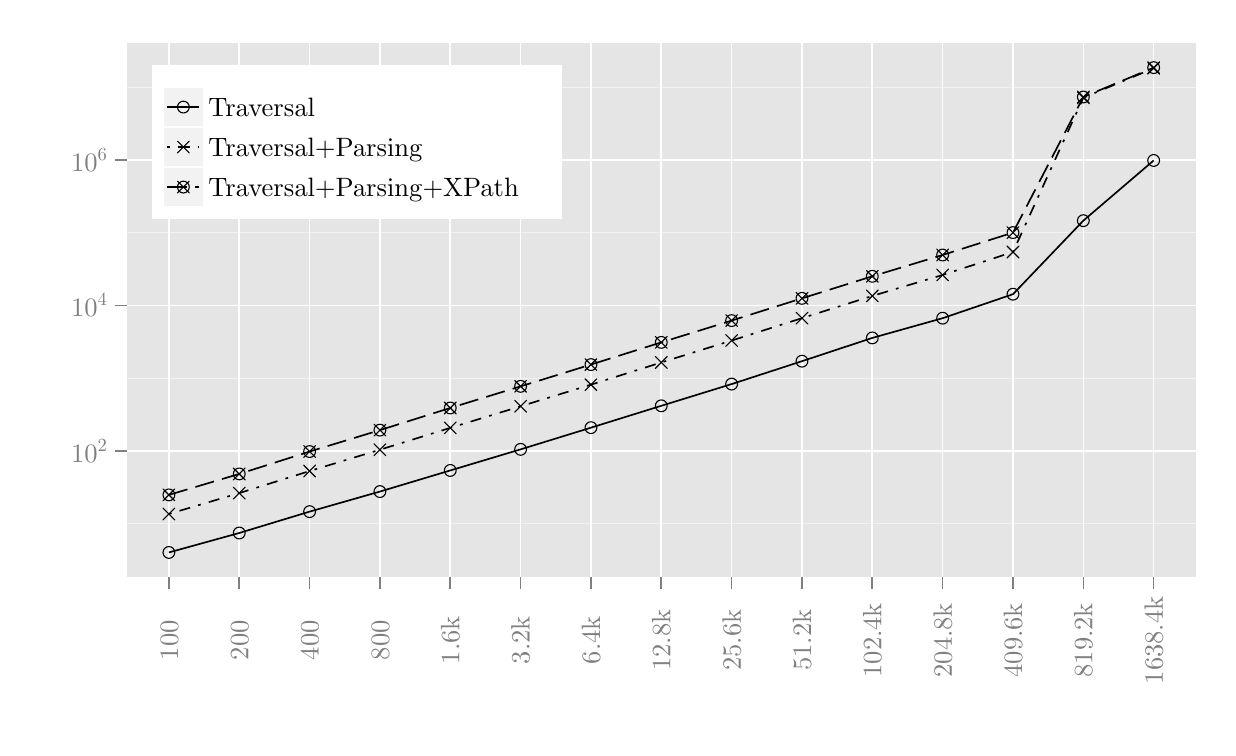
\begin{tikzpicture}[x=1pt,y=1pt]
\definecolor[named]{fillColor}{rgb}{1.00,1.00,1.00}
\path[use as bounding box,fill=fillColor,fill opacity=0.00] (0,0) rectangle (426.39,252.94);
\begin{scope}
\path[clip] (  0.00,  0.00) rectangle (426.39,252.94);
\definecolor[named]{drawColor}{rgb}{1.00,1.00,1.00}
\definecolor[named]{fillColor}{rgb}{1.00,1.00,1.00}

\path[draw=drawColor,line width= 0.6pt,line join=round,line cap=round,fill=fillColor] (  0.00,  0.00) rectangle (426.39,252.94);
\end{scope}
\begin{scope}
\path[clip] ( 35.78, 54.55) rectangle (422.13,247.25);
\definecolor[named]{fillColor}{rgb}{0.90,0.90,0.90}

\path[fill=fillColor] ( 35.78, 54.55) rectangle (422.13,247.25);
\definecolor[named]{drawColor}{rgb}{0.95,0.95,0.95}

\path[draw=drawColor,line width= 0.3pt,line join=round] ( 35.78, 73.82) --
	(422.13, 73.82);

\path[draw=drawColor,line width= 0.3pt,line join=round] ( 35.78,126.34) --
	(422.13,126.34);

\path[draw=drawColor,line width= 0.3pt,line join=round] ( 35.78,178.86) --
	(422.13,178.86);

\path[draw=drawColor,line width= 0.3pt,line join=round] ( 35.78,231.38) --
	(422.13,231.38);
\definecolor[named]{drawColor}{rgb}{1.00,1.00,1.00}

\path[draw=drawColor,line width= 0.6pt,line join=round] ( 35.78,100.08) --
	(422.13,100.08);

\path[draw=drawColor,line width= 0.6pt,line join=round] ( 35.78,152.60) --
	(422.13,152.60);

\path[draw=drawColor,line width= 0.6pt,line join=round] ( 35.78,205.12) --
	(422.13,205.12);

\path[draw=drawColor,line width= 0.6pt,line join=round] ( 51.03, 54.55) --
	( 51.03,247.25);

\path[draw=drawColor,line width= 0.6pt,line join=round] ( 76.45, 54.55) --
	( 76.45,247.25);

\path[draw=drawColor,line width= 0.6pt,line join=round] (101.87, 54.55) --
	(101.87,247.25);

\path[draw=drawColor,line width= 0.6pt,line join=round] (127.28, 54.55) --
	(127.28,247.25);

\path[draw=drawColor,line width= 0.6pt,line join=round] (152.70, 54.55) --
	(152.70,247.25);

\path[draw=drawColor,line width= 0.6pt,line join=round] (178.12, 54.55) --
	(178.12,247.25);

\path[draw=drawColor,line width= 0.6pt,line join=round] (203.54, 54.55) --
	(203.54,247.25);

\path[draw=drawColor,line width= 0.6pt,line join=round] (228.95, 54.55) --
	(228.95,247.25);

\path[draw=drawColor,line width= 0.6pt,line join=round] (254.37, 54.55) --
	(254.37,247.25);

\path[draw=drawColor,line width= 0.6pt,line join=round] (279.79, 54.55) --
	(279.79,247.25);

\path[draw=drawColor,line width= 0.6pt,line join=round] (305.20, 54.55) --
	(305.20,247.25);

\path[draw=drawColor,line width= 0.6pt,line join=round] (330.62, 54.55) --
	(330.62,247.25);

\path[draw=drawColor,line width= 0.6pt,line join=round] (356.04, 54.55) --
	(356.04,247.25);

\path[draw=drawColor,line width= 0.6pt,line join=round] (381.46, 54.55) --
	(381.46,247.25);

\path[draw=drawColor,line width= 0.6pt,line join=round] (406.87, 54.55) --
	(406.87,247.25);
\definecolor[named]{drawColor}{rgb}{0.00,0.00,0.00}

\path[draw=drawColor,line width= 0.6pt,line join=round] ( 51.03, 63.31) --
	( 76.45, 70.34) --
	(101.87, 78.06) --
	(127.28, 85.31) --
	(152.70, 92.94) --
	(178.12,100.56) --
	(203.54,108.40) --
	(228.95,116.30) --
	(254.37,124.15) --
	(279.79,132.42) --
	(305.20,140.83) --
	(330.62,147.96) --
	(356.04,156.63) --
	(381.46,183.20) --
	(406.87,204.95);

\path[draw=drawColor,line width= 0.6pt,dash pattern=on 1pt off 3pt on 4pt off 3pt ,line join=round] ( 51.03, 77.22) --
	( 76.45, 84.75) --
	(101.87, 92.73) --
	(127.28,100.43) --
	(152.70,108.32) --
	(178.12,116.12) --
	(203.54,123.94) --
	(228.95,131.96) --
	(254.37,139.88) --
	(279.79,147.97) --
	(305.20,156.00) --
	(330.62,163.58) --
	(356.04,171.87) --
	(381.46,227.61) --
	(406.87,238.28);

\path[draw=drawColor,line width= 0.6pt,dash pattern=on 7pt off 3pt ,line join=round] ( 51.03, 84.11) --
	( 76.45, 91.68) --
	(101.87, 99.77) --
	(127.28,107.51) --
	(152.70,115.51) --
	(178.12,123.33) --
	(203.54,131.20) --
	(228.95,139.22) --
	(254.37,147.09) --
	(279.79,155.13) --
	(305.20,163.10) --
	(330.62,170.79) --
	(356.04,178.89) --
	(381.46,227.89) --
	(406.87,238.50);

\path[draw=drawColor,line width= 0.4pt,line join=round,line cap=round] ( 51.03, 63.31) circle (  2.13);

\path[draw=drawColor,line width= 0.4pt,line join=round,line cap=round] ( 76.45, 70.34) circle (  2.13);

\path[draw=drawColor,line width= 0.4pt,line join=round,line cap=round] (101.87, 78.06) circle (  2.13);

\path[draw=drawColor,line width= 0.4pt,line join=round,line cap=round] (127.28, 85.31) circle (  2.13);

\path[draw=drawColor,line width= 0.4pt,line join=round,line cap=round] (152.70, 92.94) circle (  2.13);

\path[draw=drawColor,line width= 0.4pt,line join=round,line cap=round] (178.12,100.56) circle (  2.13);

\path[draw=drawColor,line width= 0.4pt,line join=round,line cap=round] (203.54,108.40) circle (  2.13);

\path[draw=drawColor,line width= 0.4pt,line join=round,line cap=round] (228.95,116.30) circle (  2.13);

\path[draw=drawColor,line width= 0.4pt,line join=round,line cap=round] (254.37,124.15) circle (  2.13);

\path[draw=drawColor,line width= 0.4pt,line join=round,line cap=round] (279.79,132.42) circle (  2.13);

\path[draw=drawColor,line width= 0.4pt,line join=round,line cap=round] (305.20,140.83) circle (  2.13);

\path[draw=drawColor,line width= 0.4pt,line join=round,line cap=round] (330.62,147.96) circle (  2.13);

\path[draw=drawColor,line width= 0.4pt,line join=round,line cap=round] (356.04,156.63) circle (  2.13);

\path[draw=drawColor,line width= 0.4pt,line join=round,line cap=round] (381.46,183.20) circle (  2.13);

\path[draw=drawColor,line width= 0.4pt,line join=round,line cap=round] (406.87,204.95) circle (  2.13);
\definecolor[named]{fillColor}{rgb}{1.00,1.00,1.00}

\path[draw=drawColor,line width= 0.4pt,line join=round,line cap=round,fill=fillColor] ( 48.90, 75.08) -- ( 53.16, 79.35);

\path[draw=drawColor,line width= 0.4pt,line join=round,line cap=round,fill=fillColor] ( 48.90, 79.35) -- ( 53.16, 75.08);

\path[draw=drawColor,line width= 0.4pt,line join=round,line cap=round,fill=fillColor] ( 74.31, 82.61) -- ( 78.58, 86.88);

\path[draw=drawColor,line width= 0.4pt,line join=round,line cap=round,fill=fillColor] ( 74.31, 86.88) -- ( 78.58, 82.61);

\path[draw=drawColor,line width= 0.4pt,line join=round,line cap=round,fill=fillColor] ( 99.73, 90.59) -- (104.00, 94.86);

\path[draw=drawColor,line width= 0.4pt,line join=round,line cap=round,fill=fillColor] ( 99.73, 94.86) -- (104.00, 90.59);

\path[draw=drawColor,line width= 0.4pt,line join=round,line cap=round,fill=fillColor] (125.15, 98.29) -- (129.42,102.56);

\path[draw=drawColor,line width= 0.4pt,line join=round,line cap=round,fill=fillColor] (125.15,102.56) -- (129.42, 98.29);

\path[draw=drawColor,line width= 0.4pt,line join=round,line cap=round,fill=fillColor] (150.57,106.18) -- (154.83,110.45);

\path[draw=drawColor,line width= 0.4pt,line join=round,line cap=round,fill=fillColor] (150.57,110.45) -- (154.83,106.18);

\path[draw=drawColor,line width= 0.4pt,line join=round,line cap=round,fill=fillColor] (175.98,113.99) -- (180.25,118.26);

\path[draw=drawColor,line width= 0.4pt,line join=round,line cap=round,fill=fillColor] (175.98,118.26) -- (180.25,113.99);

\path[draw=drawColor,line width= 0.4pt,line join=round,line cap=round,fill=fillColor] (201.40,121.80) -- (205.67,126.07);

\path[draw=drawColor,line width= 0.4pt,line join=round,line cap=round,fill=fillColor] (201.40,126.07) -- (205.67,121.80);

\path[draw=drawColor,line width= 0.4pt,line join=round,line cap=round,fill=fillColor] (226.82,129.82) -- (231.09,134.09);

\path[draw=drawColor,line width= 0.4pt,line join=round,line cap=round,fill=fillColor] (226.82,134.09) -- (231.09,129.82);

\path[draw=drawColor,line width= 0.4pt,line join=round,line cap=round,fill=fillColor] (252.24,137.75) -- (256.50,142.02);

\path[draw=drawColor,line width= 0.4pt,line join=round,line cap=round,fill=fillColor] (252.24,142.02) -- (256.50,137.75);

\path[draw=drawColor,line width= 0.4pt,line join=round,line cap=round,fill=fillColor] (277.65,145.84) -- (281.92,150.10);

\path[draw=drawColor,line width= 0.4pt,line join=round,line cap=round,fill=fillColor] (277.65,150.10) -- (281.92,145.84);

\path[draw=drawColor,line width= 0.4pt,line join=round,line cap=round,fill=fillColor] (303.07,153.87) -- (307.34,158.14);

\path[draw=drawColor,line width= 0.4pt,line join=round,line cap=round,fill=fillColor] (303.07,158.14) -- (307.34,153.87);

\path[draw=drawColor,line width= 0.4pt,line join=round,line cap=round,fill=fillColor] (328.49,161.45) -- (332.76,165.72);

\path[draw=drawColor,line width= 0.4pt,line join=round,line cap=round,fill=fillColor] (328.49,165.72) -- (332.76,161.45);

\path[draw=drawColor,line width= 0.4pt,line join=round,line cap=round,fill=fillColor] (353.91,169.74) -- (358.17,174.01);

\path[draw=drawColor,line width= 0.4pt,line join=round,line cap=round,fill=fillColor] (353.91,174.01) -- (358.17,169.74);

\path[draw=drawColor,line width= 0.4pt,line join=round,line cap=round,fill=fillColor] (379.32,225.47) -- (383.59,229.74);

\path[draw=drawColor,line width= 0.4pt,line join=round,line cap=round,fill=fillColor] (379.32,229.74) -- (383.59,225.47);

\path[draw=drawColor,line width= 0.4pt,line join=round,line cap=round,fill=fillColor] (404.74,236.15) -- (409.01,240.42);

\path[draw=drawColor,line width= 0.4pt,line join=round,line cap=round,fill=fillColor] (404.74,240.42) -- (409.01,236.15);

\path[draw=drawColor,line width= 0.4pt,line join=round,line cap=round] ( 51.03, 84.11) circle (  2.13);

\path[draw=drawColor,line width= 0.4pt,line join=round,line cap=round] ( 48.90, 81.98) -- ( 53.16, 86.25);

\path[draw=drawColor,line width= 0.4pt,line join=round,line cap=round] ( 48.90, 86.25) -- ( 53.16, 81.98);

\path[draw=drawColor,line width= 0.4pt,line join=round,line cap=round] ( 76.45, 91.68) circle (  2.13);

\path[draw=drawColor,line width= 0.4pt,line join=round,line cap=round] ( 74.31, 89.54) -- ( 78.58, 93.81);

\path[draw=drawColor,line width= 0.4pt,line join=round,line cap=round] ( 74.31, 93.81) -- ( 78.58, 89.54);

\path[draw=drawColor,line width= 0.4pt,line join=round,line cap=round] (101.87, 99.77) circle (  2.13);

\path[draw=drawColor,line width= 0.4pt,line join=round,line cap=round] ( 99.73, 97.64) -- (104.00,101.91);

\path[draw=drawColor,line width= 0.4pt,line join=round,line cap=round] ( 99.73,101.91) -- (104.00, 97.64);

\path[draw=drawColor,line width= 0.4pt,line join=round,line cap=round] (127.28,107.51) circle (  2.13);

\path[draw=drawColor,line width= 0.4pt,line join=round,line cap=round] (125.15,105.38) -- (129.42,109.64);

\path[draw=drawColor,line width= 0.4pt,line join=round,line cap=round] (125.15,109.64) -- (129.42,105.38);

\path[draw=drawColor,line width= 0.4pt,line join=round,line cap=round] (152.70,115.51) circle (  2.13);

\path[draw=drawColor,line width= 0.4pt,line join=round,line cap=round] (150.57,113.38) -- (154.83,117.64);

\path[draw=drawColor,line width= 0.4pt,line join=round,line cap=round] (150.57,117.64) -- (154.83,113.38);

\path[draw=drawColor,line width= 0.4pt,line join=round,line cap=round] (178.12,123.33) circle (  2.13);

\path[draw=drawColor,line width= 0.4pt,line join=round,line cap=round] (175.98,121.20) -- (180.25,125.47);

\path[draw=drawColor,line width= 0.4pt,line join=round,line cap=round] (175.98,125.47) -- (180.25,121.20);

\path[draw=drawColor,line width= 0.4pt,line join=round,line cap=round] (203.54,131.20) circle (  2.13);

\path[draw=drawColor,line width= 0.4pt,line join=round,line cap=round] (201.40,129.06) -- (205.67,133.33);

\path[draw=drawColor,line width= 0.4pt,line join=round,line cap=round] (201.40,133.33) -- (205.67,129.06);

\path[draw=drawColor,line width= 0.4pt,line join=round,line cap=round] (228.95,139.22) circle (  2.13);

\path[draw=drawColor,line width= 0.4pt,line join=round,line cap=round] (226.82,137.08) -- (231.09,141.35);

\path[draw=drawColor,line width= 0.4pt,line join=round,line cap=round] (226.82,141.35) -- (231.09,137.08);

\path[draw=drawColor,line width= 0.4pt,line join=round,line cap=round] (254.37,147.09) circle (  2.13);

\path[draw=drawColor,line width= 0.4pt,line join=round,line cap=round] (252.24,144.96) -- (256.50,149.23);

\path[draw=drawColor,line width= 0.4pt,line join=round,line cap=round] (252.24,149.23) -- (256.50,144.96);

\path[draw=drawColor,line width= 0.4pt,line join=round,line cap=round] (279.79,155.13) circle (  2.13);

\path[draw=drawColor,line width= 0.4pt,line join=round,line cap=round] (277.65,153.00) -- (281.92,157.26);

\path[draw=drawColor,line width= 0.4pt,line join=round,line cap=round] (277.65,157.26) -- (281.92,153.00);

\path[draw=drawColor,line width= 0.4pt,line join=round,line cap=round] (305.20,163.10) circle (  2.13);

\path[draw=drawColor,line width= 0.4pt,line join=round,line cap=round] (303.07,160.96) -- (307.34,165.23);

\path[draw=drawColor,line width= 0.4pt,line join=round,line cap=round] (303.07,165.23) -- (307.34,160.96);

\path[draw=drawColor,line width= 0.4pt,line join=round,line cap=round] (330.62,170.79) circle (  2.13);

\path[draw=drawColor,line width= 0.4pt,line join=round,line cap=round] (328.49,168.66) -- (332.76,172.93);

\path[draw=drawColor,line width= 0.4pt,line join=round,line cap=round] (328.49,172.93) -- (332.76,168.66);

\path[draw=drawColor,line width= 0.4pt,line join=round,line cap=round] (356.04,178.89) circle (  2.13);

\path[draw=drawColor,line width= 0.4pt,line join=round,line cap=round] (353.91,176.75) -- (358.17,181.02);

\path[draw=drawColor,line width= 0.4pt,line join=round,line cap=round] (353.91,181.02) -- (358.17,176.75);

\path[draw=drawColor,line width= 0.4pt,line join=round,line cap=round] (381.46,227.89) circle (  2.13);

\path[draw=drawColor,line width= 0.4pt,line join=round,line cap=round] (379.32,225.76) -- (383.59,230.02);

\path[draw=drawColor,line width= 0.4pt,line join=round,line cap=round] (379.32,230.02) -- (383.59,225.76);

\path[draw=drawColor,line width= 0.4pt,line join=round,line cap=round] (406.87,238.50) circle (  2.13);

\path[draw=drawColor,line width= 0.4pt,line join=round,line cap=round] (404.74,236.36) -- (409.01,240.63);

\path[draw=drawColor,line width= 0.4pt,line join=round,line cap=round] (404.74,240.63) -- (409.01,236.36);
\end{scope}
\begin{scope}
\path[clip] (  0.00,  0.00) rectangle (426.39,252.94);
\definecolor[named]{drawColor}{rgb}{0.50,0.50,0.50}

\node[text=drawColor,anchor=base west,inner sep=0pt, outer sep=0pt, scale=  0.96] at ( 15.71, 95.96) {10};

\node[text=drawColor,anchor=base west,inner sep=0pt, outer sep=0pt, scale=  0.67] at ( 25.31, 99.88) {2};

\node[text=drawColor,anchor=base west,inner sep=0pt, outer sep=0pt, scale=  0.96] at ( 15.71,148.48) {10};

\node[text=drawColor,anchor=base west,inner sep=0pt, outer sep=0pt, scale=  0.67] at ( 25.31,152.40) {4};

\node[text=drawColor,anchor=base west,inner sep=0pt, outer sep=0pt, scale=  0.96] at ( 15.71,201.00) {10};

\node[text=drawColor,anchor=base west,inner sep=0pt, outer sep=0pt, scale=  0.67] at ( 25.31,204.93) {6};
\end{scope}
\begin{scope}
\path[clip] (  0.00,  0.00) rectangle (426.39,252.94);
\definecolor[named]{drawColor}{rgb}{0.50,0.50,0.50}

\path[draw=drawColor,line width= 0.6pt,line join=round] ( 31.51,100.08) --
	( 35.78,100.08);

\path[draw=drawColor,line width= 0.6pt,line join=round] ( 31.51,152.60) --
	( 35.78,152.60);

\path[draw=drawColor,line width= 0.6pt,line join=round] ( 31.51,205.12) --
	( 35.78,205.12);
\end{scope}
\begin{scope}
\path[clip] (  0.00,  0.00) rectangle (426.39,252.94);
\definecolor[named]{drawColor}{rgb}{0.50,0.50,0.50}

\path[draw=drawColor,line width= 0.6pt,line join=round] ( 51.03, 50.28) --
	( 51.03, 54.55);

\path[draw=drawColor,line width= 0.6pt,line join=round] ( 76.45, 50.28) --
	( 76.45, 54.55);

\path[draw=drawColor,line width= 0.6pt,line join=round] (101.87, 50.28) --
	(101.87, 54.55);

\path[draw=drawColor,line width= 0.6pt,line join=round] (127.28, 50.28) --
	(127.28, 54.55);

\path[draw=drawColor,line width= 0.6pt,line join=round] (152.70, 50.28) --
	(152.70, 54.55);

\path[draw=drawColor,line width= 0.6pt,line join=round] (178.12, 50.28) --
	(178.12, 54.55);

\path[draw=drawColor,line width= 0.6pt,line join=round] (203.54, 50.28) --
	(203.54, 54.55);

\path[draw=drawColor,line width= 0.6pt,line join=round] (228.95, 50.28) --
	(228.95, 54.55);

\path[draw=drawColor,line width= 0.6pt,line join=round] (254.37, 50.28) --
	(254.37, 54.55);

\path[draw=drawColor,line width= 0.6pt,line join=round] (279.79, 50.28) --
	(279.79, 54.55);

\path[draw=drawColor,line width= 0.6pt,line join=round] (305.20, 50.28) --
	(305.20, 54.55);

\path[draw=drawColor,line width= 0.6pt,line join=round] (330.62, 50.28) --
	(330.62, 54.55);

\path[draw=drawColor,line width= 0.6pt,line join=round] (356.04, 50.28) --
	(356.04, 54.55);

\path[draw=drawColor,line width= 0.6pt,line join=round] (381.46, 50.28) --
	(381.46, 54.55);

\path[draw=drawColor,line width= 0.6pt,line join=round] (406.87, 50.28) --
	(406.87, 54.55);
\end{scope}
\begin{scope}
\path[clip] (  0.00,  0.00) rectangle (426.39,252.94);
\definecolor[named]{drawColor}{rgb}{0.50,0.50,0.50}

\node[text=drawColor,rotate= 90.00,anchor=base,inner sep=0pt, outer sep=0pt, scale=  0.96] at ( 54.34, 31.57) {100};

\node[text=drawColor,rotate= 90.00,anchor=base,inner sep=0pt, outer sep=0pt, scale=  0.96] at ( 79.75, 31.57) {200};

\node[text=drawColor,rotate= 90.00,anchor=base,inner sep=0pt, outer sep=0pt, scale=  0.96] at (105.17, 31.57) {400};

\node[text=drawColor,rotate= 90.00,anchor=base,inner sep=0pt, outer sep=0pt, scale=  0.96] at (130.59, 31.57) {800};

\node[text=drawColor,rotate= 90.00,anchor=base,inner sep=0pt, outer sep=0pt, scale=  0.96] at (156.01, 31.57) {1.6k};

\node[text=drawColor,rotate= 90.00,anchor=base,inner sep=0pt, outer sep=0pt, scale=  0.96] at (181.42, 31.57) {3.2k};

\node[text=drawColor,rotate= 90.00,anchor=base,inner sep=0pt, outer sep=0pt, scale=  0.96] at (206.84, 31.57) {6.4k};

\node[text=drawColor,rotate= 90.00,anchor=base,inner sep=0pt, outer sep=0pt, scale=  0.96] at (232.26, 31.57) {12.8k};

\node[text=drawColor,rotate= 90.00,anchor=base,inner sep=0pt, outer sep=0pt, scale=  0.96] at (257.68, 31.57) {25.6k};

\node[text=drawColor,rotate= 90.00,anchor=base,inner sep=0pt, outer sep=0pt, scale=  0.96] at (283.09, 31.57) {51.2k};

\node[text=drawColor,rotate= 90.00,anchor=base,inner sep=0pt, outer sep=0pt, scale=  0.96] at (308.51, 31.57) {102.4k};

\node[text=drawColor,rotate= 90.00,anchor=base,inner sep=0pt, outer sep=0pt, scale=  0.96] at (333.93, 31.57) {204.8k};

\node[text=drawColor,rotate= 90.00,anchor=base,inner sep=0pt, outer sep=0pt, scale=  0.96] at (359.35, 31.57) {409.6k};

\node[text=drawColor,rotate= 90.00,anchor=base,inner sep=0pt, outer sep=0pt, scale=  0.96] at (384.76, 31.57) {819.2k};

\node[text=drawColor,rotate= 90.00,anchor=base,inner sep=0pt, outer sep=0pt, scale=  0.96] at (410.18, 31.57) {1638.4k};
\end{scope}
\begin{scope}
\path[clip] (  0.00,  0.00) rectangle (426.39,252.94);
\definecolor[named]{fillColor}{rgb}{1.00,1.00,1.00}

\path[fill=fillColor] ( 44.77,183.85) rectangle (192.92,239.36);
\end{scope}
\begin{scope}
\path[clip] (  0.00,  0.00) rectangle (426.39,252.94);
\definecolor[named]{drawColor}{rgb}{1.00,1.00,1.00}
\definecolor[named]{fillColor}{rgb}{0.95,0.95,0.95}

\path[draw=drawColor,line width= 0.6pt,line join=round,line cap=round,fill=fillColor] ( 49.03,217.02) rectangle ( 63.49,231.48);
\end{scope}
\begin{scope}
\path[clip] (  0.00,  0.00) rectangle (426.39,252.94);
\definecolor[named]{drawColor}{rgb}{0.00,0.00,0.00}

\path[draw=drawColor,line width= 0.6pt,line join=round] ( 50.48,224.25) -- ( 62.04,224.25);
\end{scope}
\begin{scope}
\path[clip] (  0.00,  0.00) rectangle (426.39,252.94);
\definecolor[named]{drawColor}{rgb}{0.00,0.00,0.00}

\path[draw=drawColor,line width= 0.4pt,line join=round,line cap=round] ( 56.26,224.25) circle (  2.13);
\end{scope}
\begin{scope}
\path[clip] (  0.00,  0.00) rectangle (426.39,252.94);
\definecolor[named]{drawColor}{rgb}{1.00,1.00,1.00}
\definecolor[named]{fillColor}{rgb}{0.95,0.95,0.95}

\path[draw=drawColor,line width= 0.6pt,line join=round,line cap=round,fill=fillColor] ( 49.03,202.57) rectangle ( 63.49,217.02);
\end{scope}
\begin{scope}
\path[clip] (  0.00,  0.00) rectangle (426.39,252.94);
\definecolor[named]{drawColor}{rgb}{0.00,0.00,0.00}

\path[draw=drawColor,line width= 0.6pt,dash pattern=on 1pt off 3pt on 4pt off 3pt ,line join=round] ( 50.48,209.80) -- ( 62.04,209.80);
\end{scope}
\begin{scope}
\path[clip] (  0.00,  0.00) rectangle (426.39,252.94);
\definecolor[named]{drawColor}{rgb}{0.00,0.00,0.00}
\definecolor[named]{fillColor}{rgb}{1.00,1.00,1.00}

\path[draw=drawColor,line width= 0.4pt,line join=round,line cap=round,fill=fillColor] ( 54.13,207.66) -- ( 58.40,211.93);

\path[draw=drawColor,line width= 0.4pt,line join=round,line cap=round,fill=fillColor] ( 54.13,211.93) -- ( 58.40,207.66);
\end{scope}
\begin{scope}
\path[clip] (  0.00,  0.00) rectangle (426.39,252.94);
\definecolor[named]{drawColor}{rgb}{1.00,1.00,1.00}
\definecolor[named]{fillColor}{rgb}{0.95,0.95,0.95}

\path[draw=drawColor,line width= 0.6pt,line join=round,line cap=round,fill=fillColor] ( 49.03,188.12) rectangle ( 63.49,202.57);
\end{scope}
\begin{scope}
\path[clip] (  0.00,  0.00) rectangle (426.39,252.94);
\definecolor[named]{drawColor}{rgb}{0.00,0.00,0.00}

\path[draw=drawColor,line width= 0.6pt,dash pattern=on 7pt off 3pt ,line join=round] ( 50.48,195.34) -- ( 62.04,195.34);
\end{scope}
\begin{scope}
\path[clip] (  0.00,  0.00) rectangle (426.39,252.94);
\definecolor[named]{drawColor}{rgb}{0.00,0.00,0.00}

\path[draw=drawColor,line width= 0.4pt,line join=round,line cap=round] ( 56.26,195.34) circle (  2.13);

\path[draw=drawColor,line width= 0.4pt,line join=round,line cap=round] ( 54.13,193.21) -- ( 58.40,197.48);

\path[draw=drawColor,line width= 0.4pt,line join=round,line cap=round] ( 54.13,197.48) -- ( 58.40,193.21);
\end{scope}
\begin{scope}
\path[clip] (  0.00,  0.00) rectangle (426.39,252.94);
\definecolor[named]{drawColor}{rgb}{0.00,0.00,0.00}

\node[text=drawColor,anchor=base west,inner sep=0pt, outer sep=0pt, scale=  0.96] at ( 65.29,220.95) {Traversal $\;\;\;$};
\end{scope}
\begin{scope}
\path[clip] (  0.00,  0.00) rectangle (426.39,252.94);
\definecolor[named]{drawColor}{rgb}{0.00,0.00,0.00}

\node[text=drawColor,anchor=base west,inner sep=0pt, outer sep=0pt, scale=  0.96] at ( 65.29,206.49) {Traversal+Parsing $\;\;\;$};
\end{scope}
\begin{scope}
\path[clip] (  0.00,  0.00) rectangle (426.39,252.94);
\definecolor[named]{drawColor}{rgb}{0.00,0.00,0.00}

\node[text=drawColor,anchor=base west,inner sep=0pt, outer sep=0pt, scale=  0.96] at ( 65.29,192.04) {Traversal+Parsing+XPath $\;\;\;$};
\end{scope}
\end{tikzpicture}

% }
% \caption[Cumulative search\index{Search} query processing times]{The cumulative times taken for the different search\index{Search} query processing phases---directory traversal, XML\index{XML} parsing\index{Parsing} and XPath\index{XPath} query times.}
% \label{fig:experimentation:performance:search:processing-phases-cumulative}
%\end{figure}

%\begin{figure}
% \centering
% \framebox[\textwidth]{%
%% Created by tikzDevice version 0.6.2-92-0ad2792 on 2013-03-11 01:35:55
% !TEX encoding = UTF-8 Unicode
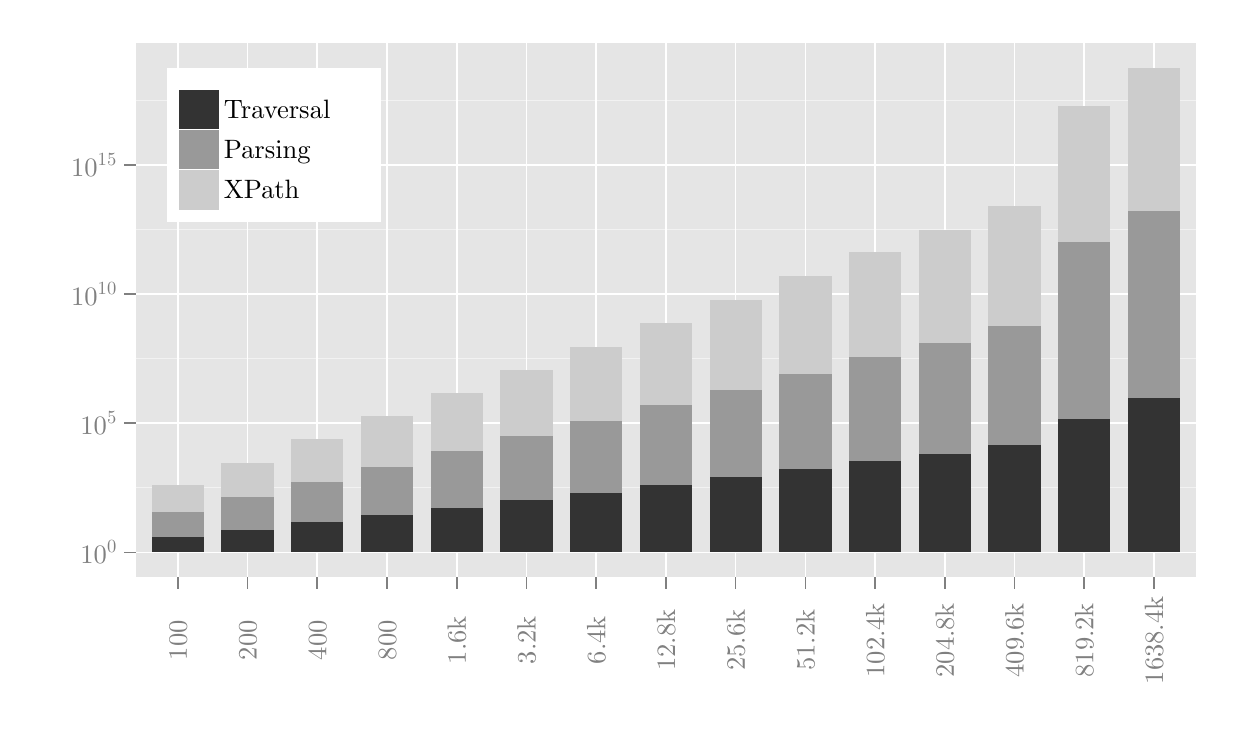
\begin{tikzpicture}[x=1pt,y=1pt]
\definecolor[named]{fillColor}{rgb}{1.00,1.00,1.00}
\path[use as bounding box,fill=fillColor,fill opacity=0.00] (0,0) rectangle (426.39,252.94);
\begin{scope}
\path[clip] (  0.00,  0.00) rectangle (426.39,252.94);
\definecolor[named]{drawColor}{rgb}{1.00,1.00,1.00}
\definecolor[named]{fillColor}{rgb}{1.00,1.00,1.00}

\path[draw=drawColor,line width= 0.6pt,line join=round,line cap=round,fill=fillColor] (  0.00, -0.00) rectangle (426.39,252.95);
\end{scope}
\begin{scope}
\path[clip] ( 39.14, 54.55) rectangle (422.13,247.25);
\definecolor[named]{fillColor}{rgb}{0.90,0.90,0.90}

\path[fill=fillColor] ( 39.14, 54.55) rectangle (422.13,247.25);
\definecolor[named]{drawColor}{rgb}{0.95,0.95,0.95}

\path[draw=drawColor,line width= 0.3pt,line join=round] ( 39.14, 86.64) --
	(422.13, 86.64);

\path[draw=drawColor,line width= 0.3pt,line join=round] ( 39.14,133.31) --
	(422.13,133.31);

\path[draw=drawColor,line width= 0.3pt,line join=round] ( 39.14,179.97) --
	(422.13,179.97);

\path[draw=drawColor,line width= 0.3pt,line join=round] ( 39.14,226.64) --
	(422.13,226.64);
\definecolor[named]{drawColor}{rgb}{1.00,1.00,1.00}

\path[draw=drawColor,line width= 0.6pt,line join=round] ( 39.14, 63.31) --
	(422.13, 63.31);

\path[draw=drawColor,line width= 0.6pt,line join=round] ( 39.14,109.97) --
	(422.13,109.97);

\path[draw=drawColor,line width= 0.6pt,line join=round] ( 39.14,156.64) --
	(422.13,156.64);

\path[draw=drawColor,line width= 0.6pt,line join=round] ( 39.14,203.31) --
	(422.13,203.31);

\path[draw=drawColor,line width= 0.6pt,line join=round] ( 54.26, 54.55) --
	( 54.26,247.25);

\path[draw=drawColor,line width= 0.6pt,line join=round] ( 79.45, 54.55) --
	( 79.45,247.25);

\path[draw=drawColor,line width= 0.6pt,line join=round] (104.65, 54.55) --
	(104.65,247.25);

\path[draw=drawColor,line width= 0.6pt,line join=round] (129.85, 54.55) --
	(129.85,247.25);

\path[draw=drawColor,line width= 0.6pt,line join=round] (155.04, 54.55) --
	(155.04,247.25);

\path[draw=drawColor,line width= 0.6pt,line join=round] (180.24, 54.55) --
	(180.24,247.25);

\path[draw=drawColor,line width= 0.6pt,line join=round] (205.44, 54.55) --
	(205.44,247.25);

\path[draw=drawColor,line width= 0.6pt,line join=round] (230.63, 54.55) --
	(230.63,247.25);

\path[draw=drawColor,line width= 0.6pt,line join=round] (255.83, 54.55) --
	(255.83,247.25);

\path[draw=drawColor,line width= 0.6pt,line join=round] (281.02, 54.55) --
	(281.02,247.25);

\path[draw=drawColor,line width= 0.6pt,line join=round] (306.22, 54.55) --
	(306.22,247.25);

\path[draw=drawColor,line width= 0.6pt,line join=round] (331.42, 54.55) --
	(331.42,247.25);

\path[draw=drawColor,line width= 0.6pt,line join=round] (356.61, 54.55) --
	(356.61,247.25);

\path[draw=drawColor,line width= 0.6pt,line join=round] (381.81, 54.55) --
	(381.81,247.25);

\path[draw=drawColor,line width= 0.6pt,line join=round] (407.01, 54.55) --
	(407.01,247.25);
\definecolor[named]{fillColor}{rgb}{0.20,0.20,0.20}

\path[fill=fillColor] ( 44.81, 63.31) rectangle ( 63.71, 68.91);
\definecolor[named]{fillColor}{rgb}{0.60,0.60,0.60}

\path[fill=fillColor] ( 44.81, 68.91) rectangle ( 63.71, 78.03);
\definecolor[named]{fillColor}{rgb}{0.80,0.80,0.80}

\path[fill=fillColor] ( 44.81, 78.03) rectangle ( 63.71, 87.82);
\definecolor[named]{fillColor}{rgb}{0.20,0.20,0.20}

\path[fill=fillColor] ( 70.00, 63.31) rectangle ( 88.90, 71.41);
\definecolor[named]{fillColor}{rgb}{0.60,0.60,0.60}

\path[fill=fillColor] ( 70.00, 71.41) rectangle ( 88.90, 83.28);
\definecolor[named]{fillColor}{rgb}{0.80,0.80,0.80}

\path[fill=fillColor] ( 70.00, 83.28) rectangle ( 88.90, 95.77);
\definecolor[named]{fillColor}{rgb}{0.20,0.20,0.20}

\path[fill=fillColor] ( 95.20, 63.31) rectangle (114.10, 74.15);
\definecolor[named]{fillColor}{rgb}{0.60,0.60,0.60}

\path[fill=fillColor] ( 95.20, 74.15) rectangle (114.10, 88.89);
\definecolor[named]{fillColor}{rgb}{0.80,0.80,0.80}

\path[fill=fillColor] ( 95.20, 88.89) rectangle (114.10,104.31);
\definecolor[named]{fillColor}{rgb}{0.20,0.20,0.20}

\path[fill=fillColor] (120.40, 63.31) rectangle (139.29, 76.73);
\definecolor[named]{fillColor}{rgb}{0.60,0.60,0.60}

\path[fill=fillColor] (120.40, 76.73) rectangle (139.29, 94.27);
\definecolor[named]{fillColor}{rgb}{0.80,0.80,0.80}

\path[fill=fillColor] (120.40, 94.27) rectangle (139.29,112.45);
\definecolor[named]{fillColor}{rgb}{0.20,0.20,0.20}

\path[fill=fillColor] (145.59, 63.31) rectangle (164.49, 79.44);
\definecolor[named]{fillColor}{rgb}{0.60,0.60,0.60}

\path[fill=fillColor] (145.59, 79.44) rectangle (164.49, 99.81);
\definecolor[named]{fillColor}{rgb}{0.80,0.80,0.80}

\path[fill=fillColor] (145.59, 99.81) rectangle (164.49,120.89);
\definecolor[named]{fillColor}{rgb}{0.20,0.20,0.20}

\path[fill=fillColor] (170.79, 63.31) rectangle (189.69, 82.15);
\definecolor[named]{fillColor}{rgb}{0.60,0.60,0.60}

\path[fill=fillColor] (170.79, 82.15) rectangle (189.69,105.32);
\definecolor[named]{fillColor}{rgb}{0.80,0.80,0.80}

\path[fill=fillColor] (170.79,105.32) rectangle (189.69,129.18);
\definecolor[named]{fillColor}{rgb}{0.20,0.20,0.20}

\path[fill=fillColor] (195.99, 63.31) rectangle (214.88, 84.93);
\definecolor[named]{fillColor}{rgb}{0.60,0.60,0.60}

\path[fill=fillColor] (195.99, 84.93) rectangle (214.88,110.88);
\definecolor[named]{fillColor}{rgb}{0.80,0.80,0.80}

\path[fill=fillColor] (195.99,110.88) rectangle (214.88,137.55);
\definecolor[named]{fillColor}{rgb}{0.20,0.20,0.20}

\path[fill=fillColor] (221.18, 63.31) rectangle (240.08, 87.74);
\definecolor[named]{fillColor}{rgb}{0.60,0.60,0.60}

\path[fill=fillColor] (221.18, 87.74) rectangle (240.08,116.55);
\definecolor[named]{fillColor}{rgb}{0.80,0.80,0.80}

\path[fill=fillColor] (221.18,116.55) rectangle (240.08,146.08);
\definecolor[named]{fillColor}{rgb}{0.20,0.20,0.20}

\path[fill=fillColor] (246.38, 63.31) rectangle (265.28, 90.53);
\definecolor[named]{fillColor}{rgb}{0.60,0.60,0.60}

\path[fill=fillColor] (246.38, 90.53) rectangle (265.28,122.17);
\definecolor[named]{fillColor}{rgb}{0.80,0.80,0.80}

\path[fill=fillColor] (246.38,122.17) rectangle (265.28,154.47);
\definecolor[named]{fillColor}{rgb}{0.20,0.20,0.20}

\path[fill=fillColor] (271.58, 63.31) rectangle (290.47, 93.47);
\definecolor[named]{fillColor}{rgb}{0.60,0.60,0.60}

\path[fill=fillColor] (271.58, 93.47) rectangle (290.47,127.96);
\definecolor[named]{fillColor}{rgb}{0.80,0.80,0.80}

\path[fill=fillColor] (271.58,127.96) rectangle (290.47,163.10);
\definecolor[named]{fillColor}{rgb}{0.20,0.20,0.20}

\path[fill=fillColor] (296.77, 63.31) rectangle (315.67, 96.46);
\definecolor[named]{fillColor}{rgb}{0.60,0.60,0.60}

\path[fill=fillColor] (296.77, 96.46) rectangle (315.67,133.76);
\definecolor[named]{fillColor}{rgb}{0.80,0.80,0.80}

\path[fill=fillColor] (296.77,133.76) rectangle (315.67,171.70);
\definecolor[named]{fillColor}{rgb}{0.20,0.20,0.20}

\path[fill=fillColor] (321.97, 63.31) rectangle (340.87, 98.99);
\definecolor[named]{fillColor}{rgb}{0.60,0.60,0.60}

\path[fill=fillColor] (321.97, 98.99) rectangle (340.87,139.04);
\definecolor[named]{fillColor}{rgb}{0.80,0.80,0.80}

\path[fill=fillColor] (321.97,139.04) rectangle (340.87,179.77);
\definecolor[named]{fillColor}{rgb}{0.20,0.20,0.20}

\path[fill=fillColor] (347.17, 63.31) rectangle (366.06,102.07);
\definecolor[named]{fillColor}{rgb}{0.60,0.60,0.60}

\path[fill=fillColor] (347.17,102.07) rectangle (366.06,145.02);
\definecolor[named]{fillColor}{rgb}{0.80,0.80,0.80}

\path[fill=fillColor] (347.17,145.02) rectangle (366.06,188.55);
\definecolor[named]{fillColor}{rgb}{0.20,0.20,0.20}

\path[fill=fillColor] (372.36, 63.31) rectangle (391.26,111.52);
\definecolor[named]{fillColor}{rgb}{0.60,0.60,0.60}

\path[fill=fillColor] (372.36,111.52) rectangle (391.26,175.43);
\definecolor[named]{fillColor}{rgb}{0.80,0.80,0.80}

\path[fill=fillColor] (372.36,175.43) rectangle (391.26,224.47);
\definecolor[named]{fillColor}{rgb}{0.20,0.20,0.20}

\path[fill=fillColor] (397.56, 63.31) rectangle (416.46,119.25);
\definecolor[named]{fillColor}{rgb}{0.60,0.60,0.60}

\path[fill=fillColor] (397.56,119.25) rectangle (416.46,186.81);
\definecolor[named]{fillColor}{rgb}{0.80,0.80,0.80}

\path[fill=fillColor] (397.56,186.81) rectangle (416.46,238.50);
\end{scope}
\begin{scope}
\path[clip] (  0.00,  0.00) rectangle (426.39,252.94);
\definecolor[named]{drawColor}{rgb}{0.50,0.50,0.50}

\node[text=drawColor,anchor=base west,inner sep=0pt, outer sep=0pt, scale=  0.96] at ( 19.07, 59.19) {10};

\node[text=drawColor,anchor=base west,inner sep=0pt, outer sep=0pt, scale=  0.67] at ( 28.67, 63.12) {0};

\node[text=drawColor,anchor=base west,inner sep=0pt, outer sep=0pt, scale=  0.96] at ( 19.07,105.86) {10};

\node[text=drawColor,anchor=base west,inner sep=0pt, outer sep=0pt, scale=  0.67] at ( 28.67,109.78) {5};

\node[text=drawColor,anchor=base west,inner sep=0pt, outer sep=0pt, scale=  0.96] at ( 15.71,152.52) {10};

\node[text=drawColor,anchor=base west,inner sep=0pt, outer sep=0pt, scale=  0.67] at ( 25.31,156.45) {1};

\node[text=drawColor,anchor=base west,inner sep=0pt, outer sep=0pt, scale=  0.67] at ( 28.67,156.45) {0};

\node[text=drawColor,anchor=base west,inner sep=0pt, outer sep=0pt, scale=  0.96] at ( 15.71,199.19) {10};

\node[text=drawColor,anchor=base west,inner sep=0pt, outer sep=0pt, scale=  0.67] at ( 25.31,203.11) {1};

\node[text=drawColor,anchor=base west,inner sep=0pt, outer sep=0pt, scale=  0.67] at ( 28.67,203.11) {5};
\end{scope}
\begin{scope}
\path[clip] (  0.00,  0.00) rectangle (426.39,252.94);
\definecolor[named]{drawColor}{rgb}{0.50,0.50,0.50}

\path[draw=drawColor,line width= 0.6pt,line join=round] ( 34.87, 63.31) --
	( 39.14, 63.31);

\path[draw=drawColor,line width= 0.6pt,line join=round] ( 34.87,109.97) --
	( 39.14,109.97);

\path[draw=drawColor,line width= 0.6pt,line join=round] ( 34.87,156.64) --
	( 39.14,156.64);

\path[draw=drawColor,line width= 0.6pt,line join=round] ( 34.87,203.31) --
	( 39.14,203.31);
\end{scope}
\begin{scope}
\path[clip] (  0.00,  0.00) rectangle (426.39,252.94);
\definecolor[named]{drawColor}{rgb}{0.50,0.50,0.50}

\path[draw=drawColor,line width= 0.6pt,line join=round] ( 54.26, 50.28) --
	( 54.26, 54.55);

\path[draw=drawColor,line width= 0.6pt,line join=round] ( 79.45, 50.28) --
	( 79.45, 54.55);

\path[draw=drawColor,line width= 0.6pt,line join=round] (104.65, 50.28) --
	(104.65, 54.55);

\path[draw=drawColor,line width= 0.6pt,line join=round] (129.85, 50.28) --
	(129.85, 54.55);

\path[draw=drawColor,line width= 0.6pt,line join=round] (155.04, 50.28) --
	(155.04, 54.55);

\path[draw=drawColor,line width= 0.6pt,line join=round] (180.24, 50.28) --
	(180.24, 54.55);

\path[draw=drawColor,line width= 0.6pt,line join=round] (205.44, 50.28) --
	(205.44, 54.55);

\path[draw=drawColor,line width= 0.6pt,line join=round] (230.63, 50.28) --
	(230.63, 54.55);

\path[draw=drawColor,line width= 0.6pt,line join=round] (255.83, 50.28) --
	(255.83, 54.55);

\path[draw=drawColor,line width= 0.6pt,line join=round] (281.02, 50.28) --
	(281.02, 54.55);

\path[draw=drawColor,line width= 0.6pt,line join=round] (306.22, 50.28) --
	(306.22, 54.55);

\path[draw=drawColor,line width= 0.6pt,line join=round] (331.42, 50.28) --
	(331.42, 54.55);

\path[draw=drawColor,line width= 0.6pt,line join=round] (356.61, 50.28) --
	(356.61, 54.55);

\path[draw=drawColor,line width= 0.6pt,line join=round] (381.81, 50.28) --
	(381.81, 54.55);

\path[draw=drawColor,line width= 0.6pt,line join=round] (407.01, 50.28) --
	(407.01, 54.55);
\end{scope}
\begin{scope}
\path[clip] (  0.00,  0.00) rectangle (426.39,252.94);
\definecolor[named]{drawColor}{rgb}{0.50,0.50,0.50}

\node[text=drawColor,rotate= 90.00,anchor=base,inner sep=0pt, outer sep=0pt, scale=  0.96] at ( 57.56, 31.57) {100};

\node[text=drawColor,rotate= 90.00,anchor=base,inner sep=0pt, outer sep=0pt, scale=  0.96] at ( 82.76, 31.57) {200};

\node[text=drawColor,rotate= 90.00,anchor=base,inner sep=0pt, outer sep=0pt, scale=  0.96] at (107.96, 31.57) {400};

\node[text=drawColor,rotate= 90.00,anchor=base,inner sep=0pt, outer sep=0pt, scale=  0.96] at (133.15, 31.57) {800};

\node[text=drawColor,rotate= 90.00,anchor=base,inner sep=0pt, outer sep=0pt, scale=  0.96] at (158.35, 31.57) {1.6k};

\node[text=drawColor,rotate= 90.00,anchor=base,inner sep=0pt, outer sep=0pt, scale=  0.96] at (183.55, 31.57) {3.2k};

\node[text=drawColor,rotate= 90.00,anchor=base,inner sep=0pt, outer sep=0pt, scale=  0.96] at (208.74, 31.57) {6.4k};

\node[text=drawColor,rotate= 90.00,anchor=base,inner sep=0pt, outer sep=0pt, scale=  0.96] at (233.94, 31.57) {12.8k};

\node[text=drawColor,rotate= 90.00,anchor=base,inner sep=0pt, outer sep=0pt, scale=  0.96] at (259.13, 31.57) {25.6k};

\node[text=drawColor,rotate= 90.00,anchor=base,inner sep=0pt, outer sep=0pt, scale=  0.96] at (284.33, 31.57) {51.2k};

\node[text=drawColor,rotate= 90.00,anchor=base,inner sep=0pt, outer sep=0pt, scale=  0.96] at (309.53, 31.57) {102.4k};

\node[text=drawColor,rotate= 90.00,anchor=base,inner sep=0pt, outer sep=0pt, scale=  0.96] at (334.72, 31.57) {204.8k};

\node[text=drawColor,rotate= 90.00,anchor=base,inner sep=0pt, outer sep=0pt, scale=  0.96] at (359.92, 31.57) {409.6k};

\node[text=drawColor,rotate= 90.00,anchor=base,inner sep=0pt, outer sep=0pt, scale=  0.96] at (385.12, 31.57) {819.2k};

\node[text=drawColor,rotate= 90.00,anchor=base,inner sep=0pt, outer sep=0pt, scale=  0.96] at (410.31, 31.57) {1638.4k};
\end{scope}
\begin{scope}
\path[clip] (  0.00,  0.00) rectangle (426.39,252.94);
\definecolor[named]{fillColor}{rgb}{1.00,1.00,1.00}

\path[fill=fillColor] ( 50.35,182.88) rectangle (127.51,238.40);
\end{scope}
\begin{scope}
\path[clip] (  0.00,  0.00) rectangle (426.39,252.94);
\definecolor[named]{drawColor}{rgb}{1.00,1.00,1.00}
\definecolor[named]{fillColor}{rgb}{0.95,0.95,0.95}

\path[draw=drawColor,line width= 0.6pt,line join=round,line cap=round,fill=fillColor] ( 54.62,216.06) rectangle ( 69.07,230.51);
\end{scope}
\begin{scope}
\path[clip] (  0.00,  0.00) rectangle (426.39,252.94);
\definecolor[named]{fillColor}{rgb}{0.20,0.20,0.20}

\path[fill=fillColor] ( 54.62,216.06) rectangle ( 69.07,230.51);

\path[] ( 54.62,216.06) --
	( 69.07,230.51);
\end{scope}
\begin{scope}
\path[clip] (  0.00,  0.00) rectangle (426.39,252.94);
\definecolor[named]{drawColor}{rgb}{1.00,1.00,1.00}
\definecolor[named]{fillColor}{rgb}{0.95,0.95,0.95}

\path[draw=drawColor,line width= 0.6pt,line join=round,line cap=round,fill=fillColor] ( 54.62,201.61) rectangle ( 69.07,216.06);
\end{scope}
\begin{scope}
\path[clip] (  0.00,  0.00) rectangle (426.39,252.94);
\definecolor[named]{fillColor}{rgb}{0.60,0.60,0.60}

\path[fill=fillColor] ( 54.62,201.61) rectangle ( 69.07,216.06);

\path[] ( 54.62,201.61) --
	( 69.07,216.06);
\end{scope}
\begin{scope}
\path[clip] (  0.00,  0.00) rectangle (426.39,252.94);
\definecolor[named]{drawColor}{rgb}{1.00,1.00,1.00}
\definecolor[named]{fillColor}{rgb}{0.95,0.95,0.95}

\path[draw=drawColor,line width= 0.6pt,line join=round,line cap=round,fill=fillColor] ( 54.62,187.15) rectangle ( 69.07,201.61);
\end{scope}
\begin{scope}
\path[clip] (  0.00,  0.00) rectangle (426.39,252.94);
\definecolor[named]{fillColor}{rgb}{0.80,0.80,0.80}

\path[fill=fillColor] ( 54.62,187.15) rectangle ( 69.07,201.61);

\path[] ( 54.62,187.15) --
	( 69.07,201.61);
\end{scope}
\begin{scope}
\path[clip] (  0.00,  0.00) rectangle (426.39,252.94);
\definecolor[named]{drawColor}{rgb}{0.00,0.00,0.00}

\node[text=drawColor,anchor=base west,inner sep=0pt, outer sep=0pt, scale=  0.96] at ( 70.88,219.98) {Traversal $\;\;\;\;$};
\end{scope}
\begin{scope}
\path[clip] (  0.00,  0.00) rectangle (426.39,252.94);
\definecolor[named]{drawColor}{rgb}{0.00,0.00,0.00}

\node[text=drawColor,anchor=base west,inner sep=0pt, outer sep=0pt, scale=  0.96] at ( 70.88,205.53) {Parsing $\;\;\;\;$};
\end{scope}
\begin{scope}
\path[clip] (  0.00,  0.00) rectangle (426.39,252.94);
\definecolor[named]{drawColor}{rgb}{0.00,0.00,0.00}

\node[text=drawColor,anchor=base west,inner sep=0pt, outer sep=0pt, scale=  0.96] at ( 70.88,191.07) {XPath $\;\;\;\;$};
\end{scope}
\end{tikzpicture}

% }
% \caption[Time breakdown of search\index{Search} query processing phases]{Breakdown of time taken for the different search\index{Search} query processing phases.}
% \label{fig:experimentation:performance:search:processing-phases-distribution}
%\end{figure}


\subparagraph{Discussion}

The results in Figure~\ref{fig:experimentation:performance:search:processing-phases-cumulative} indicate an increasing linear correlation between the workload\index{Workload} size and the query response time. This is largely due to the fact that all metadata\index{Metadata} records need to be analysed each time a search\index{Search} query is issued.

In addition, Table~\ref{tab:experimentation:performance:search:processing-phases-benchmark} indicates that a significant amount of time is spent parsing\index{Parsing} and querying the records, with each of the tasks accounting for an average of \SI{39}{\percent} and \SI{46}{\percent} respectively. Furthermore, this occurs before the workload\index{Workload} size exceeds \num{409600}, at which point the parsing\index{Parsing} phase becomes extremely expensive---accounting for \SI{95}{\percent} of the total search\index{Search} query time.

%%\paragraph{Conclusion}

The query response time increases linearly as the workload\index{Workload} size is increased and is drastically affected by larger workloads.\index{Workload} The only effective way to get better performance would be to use an index.


\paragraph{Experiment: Impact of collection structure on search\index{Search} performance }
\label{sec:evaluation:performance:search-browse:experiment2}

This experiment was conducted to assess the search\index{Search} query response times relative to a collection structure. The results obtained in Section~\ref{sec:evaluation:performance:search-browse:experiment2}, derived from a one-level collection structure, were compared with workloads of varying levels.

\subparagraph{Methodology}

The search\index{Search} queries issued in Section~\ref{sec:evaluation:performance:search-browse:experiment2} were issued to two-level and a three-level, illustrated in Figure~\ref{fig:experimentation:performance:workload-design:directory-structures:dataset2} and Figure~\ref{fig:experimentation:performance:workload-design:directory-structures:dataset3} respectively, structured workloads.\index{Workload} The response times were noted and compared with those obtained from one-level structured workloads.\index{Workload}

\subparagraph{Results}

Table~\ref{tab:experimentation:performance:search:processing-phases-levels} shows the change in response times for two-level and three-level workloads relative to one-level workloads; and Figure~\ref{fig:experimentation:performance:search:processing-phases-levels} is a graphical representation of the response times for the different search\index{Search} query phases.

\tablespacing
%\begin{longtable}{p{0.12\linewidth} p{0.12\linewidth} p{0.12\linewidth}
%p{0.12\linewidth} p{0.12\linewidth} p{0.12\linewidth} p{0.12\linewidth}}
\begin{longtable}{
>{\arraybackslash}m{0.07\linewidth}|
>{\centering\arraybackslash}m{0.12\linewidth}|
>{\centering\arraybackslash}m{0.10\linewidth}|
>{\centering\arraybackslash}m{0.10\linewidth}|
>{\centering\arraybackslash}m{0.12\linewidth}|
>{\centering\arraybackslash}m{0.10\linewidth}|
>{\centering\arraybackslash}m{0.10\linewidth}}

\caption{Search query time change relative to baseline}
\label{tab:experimentation:performance:search:processing-phases-levels}\\

 %%%%%\toprule
 \hline
{} &
\multicolumn{3}{c|}{\textbf{$\Delta$ Dataset\#2}} &
\multicolumn{3}{c}{\textbf{$\Delta$ Dataset\#3}} \\
 %%%%%\midrule
\cline{2-7}
 {} & 
{\textbf{Traversal}}&
{\textbf{Parsing}}&
{\textbf{XPath}} &
{\textbf{Traversal}}&
{\textbf{Parsing}}&
{\textbf{XPath}} \\
%%%%%\midrule
\hline \hline
 \endfirsthead

 \caption[]{(continued)}\\
 %%%%%\toprule
 \hline
{} &
\multicolumn{3}{c|}{\textbf{$\Delta$ Dataset\#2}} &
\multicolumn{3}{c}{\textbf{$\Delta$ Dataset\#3}} \\
 %%%%%\midrule
 \cline{2-7}
 {} &
{\textbf{Traversal}}&
{\textbf{Parsing}}&
{\textbf{XPath}} &
{\textbf{Traversal}}&
{\textbf{Parsing}}&
{\textbf{XPath}} \\
%%%%%\midrule
\hline \hline
 \endhead

 % Page footer
 %%%%%\midrule
 \hline
 \multicolumn{7}{r}{(Continued on next page)} \\
 \endfoot

 % Last page footer
 \bottomrule
 \endlastfoot

\textbf{W1} & {\SI{62.91}{\percent}} & {\SI{0.21}{\percent}} & {\SI{0.33}{\percent}} & {\SI{141.59}{\percent}} & {\SI[bracket-negative-numbers]{-0.39}{\percent}} & {\SI{2.13}{\percent}} \\

\textbf{W2} & {\SI{55.90}{\percent}} & {\SI[bracket-negative-numbers]{-0.99}{\percent}} & {\SI{0.45}{\percent}} & {\SI{134.24}{\percent}} & {\SI[bracket-negative-numbers]{-1.98}{\percent}} & {\SI{0.63}{\percent}} \\

\textbf{W3} & {\SI{51.78}{\percent}} & {\SI{0.65}{\percent}} & {\SI{1.65}{\percent}} & {\SI{126.18}{\percent}} & {\SI[bracket-negative-numbers]{-0.84}{\percent}} & {\SI{1.68}{\percent}} \\

\textbf{W4} & {\SI{39.22}{\percent}} & {\SI{0.38}{\percent}} & {\SI{1.24}{\percent}} & {\SI{113.29}{\percent}} & {\SI[bracket-negative-numbers]{-1.03}{\percent}} & {\SI{2.49}{\percent}} \\

\textbf{W5} & {\SI{32.61}{\percent}} & {\SI{0.82}{\percent}} & {\SI{0.36}{\percent}} & {\SI{101.85}{\percent}} & {\SI[bracket-negative-numbers]{-1.16}{\percent}} & {\SI{0.90}{\percent}} \\

\textbf{W6} & {\SI{22.81}{\percent}} & {\SI{0.14}{\percent}} & {\SI{0.76}{\percent}} & {\SI{83.80}{\percent}} & {\SI[bracket-negative-numbers]{-1.08}{\percent}} & {\SI{2.01}{\percent}} \\

\textbf{W7} & {\SI{16.72}{\percent}} & {\SI{1.68}{\percent}} & {\SI[bracket-negative-numbers]{-0.24}{\percent}} & {\SI{133.23}{\percent}} & {\SI[bracket-negative-numbers]{-0.03}{\percent}} & {\SI{0.46}{\percent}} \\

\textbf{W8} & {\SI{11.03}{\percent}} & {\SI{0.40}{\percent}} & {\SI[bracket-negative-numbers]{-0.72}{\percent}} & {\SI{59.56}{\percent}} & {\SI[bracket-negative-numbers]{-0.33}{\percent}} & {\SI[bracket-negative-numbers]{-0.02}{\percent}} \\

\textbf{W9} & {\SI{6.82}{\percent}} & {\SI{0.10}{\percent}} & {\SI[bracket-negative-numbers]{-0.27}{\percent}} & {\SI{48.84}{\percent}} & {\SI[bracket-negative-numbers]{-0.55}{\percent}} & {\SI{0.39}{\percent}} \\

\textbf{W10} & {\SI{7.47}{\percent}} & {\SI[bracket-negative-numbers]{-0.88}{\percent}} & {\SI[bracket-negative-numbers]{-0.89}{\percent}} & {\SI{42.11}{\percent}} & {\SI[bracket-negative-numbers]{-0.42}{\percent}} & {\SI{0.18}{\percent}} \\

\textbf{W11} & {\SI{0.18}{\percent}} & {\SI[bracket-negative-numbers]{-0.51}{\percent}} & {\SI[bracket-negative-numbers]{-0.70}{\percent}} & {\SI{38.81}{\percent}} & {\SI{0.44}{\percent}} & {\SI[bracket-negative-numbers]{-0.34}{\percent}} \\

\textbf{W12} & {\SI{9.39}{\percent}} & {\SI{1.07}{\percent}} & {\SI[bracket-negative-numbers]{-0.10}{\percent}} & {\SI{62.04}{\percent}} & {\SI{2.54}{\percent}} & {\SI{0.79}{\percent}} \\

\textbf{W13} & {\SI{8.61}{\percent}} & {\SI{0.01}{\percent}} & {\SI{0.54}{\percent}} & {\SI{137.16}{\percent}} & {\SI{1.84}{\percent}} & {\SI{2.72}{\percent}} \\

\textbf{W14} & {\SI[bracket-negative-numbers]{-30.37}{\percent}} & {\SI[bracket-negative-numbers]{-54.99}{\percent}} & {\SI{5.10}{\percent}} & {\SI{66.06}{\percent}} & {\SI[bracket-negative-numbers]{-86.83}{\percent}} & {\SI{6.78}{\percent}} \\

\textbf{W15} & {\SI[bracket-negative-numbers]{-79.22}{\percent}} & {\SI[bracket-negative-numbers]{-39.63}{\percent}} & {\SI{1.78}{\percent}} & {\SI[bracket-negative-numbers]{-61.31}{\percent}} & {\SI[bracket-negative-numbers]{-86.39}{\percent}} & {\SI{11.56}{\percent}} \\


 %\cmidrule[0.1pt](l{0.5em}r{0.5em}){1-3}

 \end{longtable}

\bodyspacing

%%\tablespacing
%%%\begin{longtable}{p{0.12\linewidth} p{0.12\linewidth} p{0.12\linewidth}
%p{0.12\linewidth} p{0.12\linewidth} p{0.12\linewidth} p{0.12\linewidth}}
\begin{longtable}{
>{\arraybackslash}m{0.07\linewidth}|
>{\centering\arraybackslash}m{0.18\linewidth}|
>{\centering\arraybackslash}m{0.12\linewidth}| 
>{\centering\arraybackslash}m{0.10\linewidth}|
>{\centering\arraybackslash}m{0.10\linewidth}}

\caption{Baseline performance benchmarks for full-text search}
\label{tab:experimentation:performance:search:processing-phases-benchmark}\\

 %%%%%\toprule
 \hline
 {} & 
{\textbf{Time [ms]}}&
{\textbf{Traversal}}&
{\textbf{Parsing}}&
{\textbf{XPath}} \\
%%%%%\midrule
\hline \hline
 \endfirsthead

 \caption[]{(continued)}\\
 %%%%%\toprule
 \hline
 {} & 
{\textbf{Time [ms]}}&
{\textbf{Traversal}}&
{\textbf{Parsing}}&
{\textbf{XPath}} \\
%%%%%\midrule
\hline \hline
 \endhead

 % Page footer
 %%%%\midrule
 \hline
 \multicolumn{5}{r}{(Continued on next page)} \\
 \endfoot

 % Last page footer
 \bottomrule
 \endlastfoot

%%\textbf{W1} & {\SI{16.13}{\percent}} & {\SI{38.49}{\percent}} & {\SI{45.38}{\percent}} \\ 
%%\textbf{W2} & {\SI{15.40}{\percent}} & {\SI{39.05}{\percent}} & {\SI{45.54}{\percent}} \\ 
%%\textbf{W3} & {\SI{14.89}{\percent}} & {\SI{39.01}{\percent}} & {\SI{46.10}{\percent}} \\ 
%%\textbf{W4} & {\SI{14.28}{\percent}} & {\SI{39.45}{\percent}} & {\SI{46.27}{\percent}} \\ 
%%\textbf{W5} & {\SI{13.82}{\percent}} & {\SI{39.39}{\percent}} & {\SI{46.79}{\percent}} \\ 
%%\textbf{W6} & {\SI{13.58}{\percent}} & {\SI{39.58}{\percent}} & {\SI{46.84}{\percent}} \\ 
%%\textbf{W7} & {\SI{13.55}{\percent}} & {\SI{39.37}{\percent}} & {\SI{47.08}{\percent}} \\ 
%%\textbf{W8} & {\SI{13.41}{\percent}} & {\SI{39.52}{\percent}} & {\SI{47.08}{\percent}} \\ 
%%\textbf{W9} & {\SI{13.37}{\percent}} & {\SI{39.76}{\percent}} & {\SI{46.87}{\percent}} \\ 
%%\textbf{W10} & {\SI{13.66}{\percent}} & {\SI{39.72}{\percent}} & {\SI{46.63}{\percent}} \\ 
%%\textbf{W11} & {\SI{14.20}{\percent}} & {\SI{39.49}{\percent}} & {\SI{46.31}{\percent}} \\ 
%%\textbf{W12} & {\SI{13.51}{\percent}} & {\SI{39.65}{\percent}} & {\SI{46.85}{\percent}} \\ 
%%\textbf{W13} & {\SI{14.20}{\percent}} & {\SI{39.85}{\percent}} & {\SI{45.95}{\percent}} \\ 
%%\textbf{W14} & {\SI{1.99}{\percent}} & {\SI{95.57}{\percent}} & {\SI{2.44}{\percent}} \\ 
%%\textbf{W15} & {\SI{5.28}{\percent}} & {\SI{92.87}{\percent}} & {\SI{1.85}{\percent}} \\ 

\textbf{W1} & {\tablenum[table-format=6.2]{24.67}} & {\SI{16.13}{\percent}} & {\SI{38.49}{\percent}} & {\SI{45.38}{\percent}} \\ 
\textbf{W2} & {\tablenum[table-format=6.2]{47.87}} & {\SI{15.40}{\percent}} & {\SI{39.05}{\percent}} & {\SI{45.54}{\percent}} \\ 
\textbf{W3} & {\tablenum[table-format=6.2]{97.38}} & {\SI{14.89}{\percent}} & {\SI{39.01}{\percent}} & {\SI{46.10}{\percent}} \\ 
\textbf{W4} & {\tablenum[table-format=6.2]{191.90}} & {\SI{14.28}{\percent}} & {\SI{39.45}{\percent}} & {\SI{46.27}{\percent}} \\ 
\textbf{W5} & {\tablenum[table-format=6.2]{386.99}} & {\SI{13.82}{\percent}} & {\SI{39.39}{\percent}} & {\SI{46.79}{\percent}} \\ 
\textbf{W6} & {\tablenum[table-format=6.2]{768.35}} & {\SI{13.58}{\percent}} & {\SI{39.58}{\percent}} & {\SI{46.84}{\percent}} \\ 
\textbf{W7} & {\tablenum[table-format=6.2]{1531.06}} & {\SI{13.55}{\percent}} & {\SI{39.37}{\percent}} & {\SI{47.08}{\percent}} \\ 
\textbf{W8} & {\tablenum[table-format=6.2]{3093.12}} & {\SI{13.41}{\percent}} & {\SI{39.52}{\percent}} & {\SI{47.08}{\percent}} \\ 
\textbf{W9} & {\tablenum[table-format=6.2]{6172.22}} & {\SI{13.37}{\percent}} & {\SI{39.76}{\percent}} & {\SI{46.87}{\percent}} \\ 
\textbf{W10} & {\tablenum[table-format=6.2]{12487.06}} & {\SI{13.66}{\percent}} & {\SI{39.72}{\percent}} & {\SI{46.63}{\percent}} \\ 
\textbf{W11} & {\tablenum[table-format=6.2]{25108.74}} & {\SI{14.20}{\percent}} & {\SI{39.49}{\percent}} & {\SI{46.31}{\percent}} \\ 
\textbf{W12} & {\tablenum[table-format=6.2]{49301.45}} & {\SI{13.51}{\percent}} & {\SI{39.65}{\percent}} & {\SI{46.85}{\percent}} \\ 
\textbf{W13} & {\tablenum[table-format=6.2]{100267.33}} & {\SI{14.20}{\percent}} & {\SI{39.85}{\percent}} & {\SI{45.95}{\percent}} \\ 
\textbf{W14} & {\tablenum[table-format=6.2]{7365254.00}} & {\SI{1.99}{\percent}} & {\SI{95.57}{\percent}} & {\SI{2.44}{\percent}} \\ 
\textbf{W15} & {\tablenum[table-format=6.2]{18664713.65}} & {\SI{5.28}{\percent}} & {\SI{92.87}{\percent}} & {\SI{1.85}{\percent}} \\ 

 %\cmidrule[0.1pt](l{0.5em}r{0.5em}){1-3}

 \end{longtable}

%%\bodyspacing

\begin{figure}
 \centering
 \framebox[\textwidth]{%
% Created by tikzDevice version 0.6.2-92-0ad2792 on 2013-03-28 13:08:00
% !TEX encoding = UTF-8 Unicode
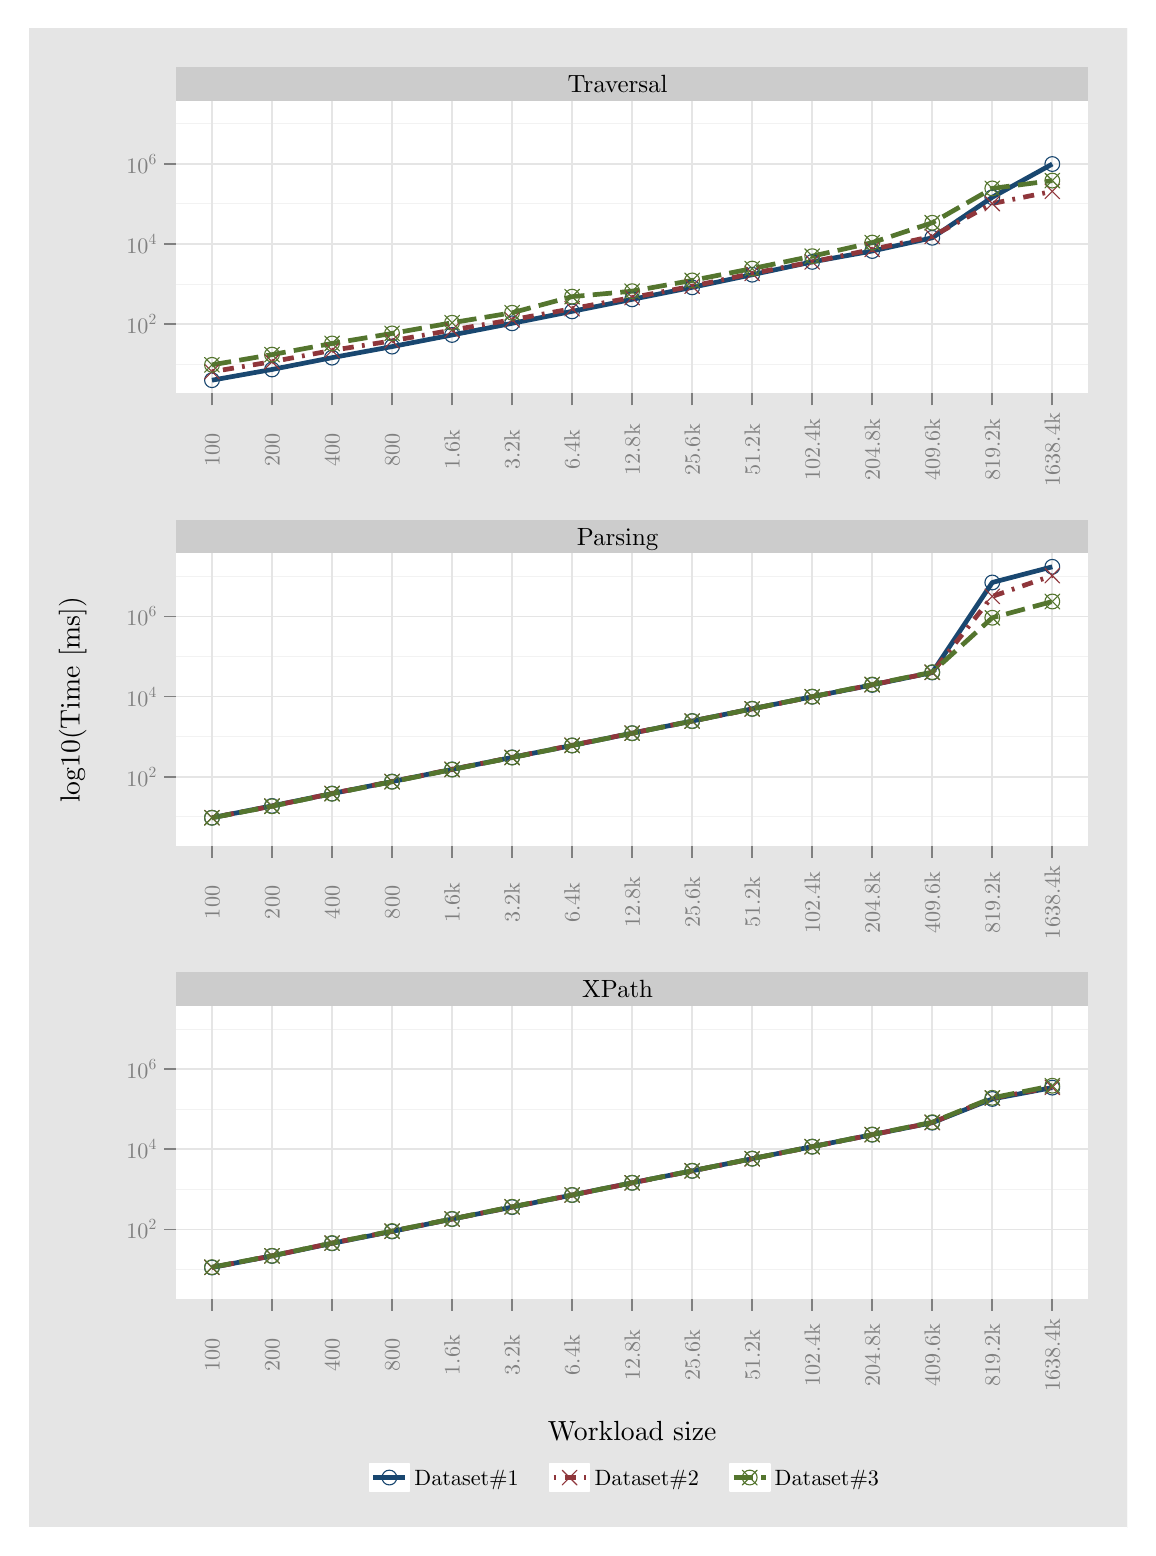
\begin{tikzpicture}[x=1pt,y=1pt]
\definecolor[named]{fillColor}{rgb}{1.00,1.00,1.00}
\path[use as bounding box,fill=fillColor,fill opacity=0.00] (0,0) rectangle (397.48,542.02);
\begin{scope}
\path[clip] (  0.00,  0.00) rectangle (397.48,542.02);
\definecolor[named]{drawColor}{rgb}{1.00,1.00,1.00}
\definecolor[named]{fillColor}{rgb}{0.90,0.90,0.90}

\path[draw=drawColor,line width= 0.6pt,line join=round,line cap=round,fill=fillColor] (  0.00,  0.00) rectangle (397.48,542.02);
\end{scope}
\begin{scope}
\path[clip] ( 53.58,409.83) rectangle (383.26,515.58);
\definecolor[named]{fillColor}{rgb}{1.00,1.00,1.00}

\path[fill=fillColor] ( 53.58,409.83) rectangle (383.26,515.58);
\definecolor[named]{drawColor}{rgb}{0.95,0.95,0.95}

\path[draw=drawColor,line width= 0.3pt,line join=round] ( 53.58,420.43) --
	(383.26,420.43);

\path[draw=drawColor,line width= 0.3pt,line join=round] ( 53.58,449.39) --
	(383.26,449.39);

\path[draw=drawColor,line width= 0.3pt,line join=round] ( 53.58,478.35) --
	(383.26,478.35);

\path[draw=drawColor,line width= 0.3pt,line join=round] ( 53.58,507.31) --
	(383.26,507.31);
\definecolor[named]{drawColor}{rgb}{0.90,0.90,0.90}

\path[draw=drawColor,line width= 0.6pt,line join=round] ( 53.58,434.91) --
	(383.26,434.91);

\path[draw=drawColor,line width= 0.6pt,line join=round] ( 53.58,463.87) --
	(383.26,463.87);

\path[draw=drawColor,line width= 0.6pt,line join=round] ( 53.58,492.83) --
	(383.26,492.83);

\path[draw=drawColor,line width= 0.6pt,line join=round] ( 66.60,409.83) --
	( 66.60,515.58);

\path[draw=drawColor,line width= 0.6pt,line join=round] ( 88.29,409.83) --
	( 88.29,515.58);

\path[draw=drawColor,line width= 0.6pt,line join=round] (109.97,409.83) --
	(109.97,515.58);

\path[draw=drawColor,line width= 0.6pt,line join=round] (131.66,409.83) --
	(131.66,515.58);

\path[draw=drawColor,line width= 0.6pt,line join=round] (153.35,409.83) --
	(153.35,515.58);

\path[draw=drawColor,line width= 0.6pt,line join=round] (175.04,409.83) --
	(175.04,515.58);

\path[draw=drawColor,line width= 0.6pt,line join=round] (196.73,409.83) --
	(196.73,515.58);

\path[draw=drawColor,line width= 0.6pt,line join=round] (218.42,409.83) --
	(218.42,515.58);

\path[draw=drawColor,line width= 0.6pt,line join=round] (240.11,409.83) --
	(240.11,515.58);

\path[draw=drawColor,line width= 0.6pt,line join=round] (261.80,409.83) --
	(261.80,515.58);

\path[draw=drawColor,line width= 0.6pt,line join=round] (283.49,409.83) --
	(283.49,515.58);

\path[draw=drawColor,line width= 0.6pt,line join=round] (305.18,409.83) --
	(305.18,515.58);

\path[draw=drawColor,line width= 0.6pt,line join=round] (326.87,409.83) --
	(326.87,515.58);

\path[draw=drawColor,line width= 0.6pt,line join=round] (348.56,409.83) --
	(348.56,515.58);

\path[draw=drawColor,line width= 0.6pt,line join=round] (370.25,409.83) --
	(370.25,515.58);
\definecolor[named]{drawColor}{rgb}{0.10,0.28,0.44}

\path[draw=drawColor,line width= 1.7pt,line join=round] ( 66.60,414.63) --
	( 88.29,418.51) --
	(109.97,422.77) --
	(131.66,426.77) --
	(153.35,430.97) --
	(175.04,435.18) --
	(196.73,439.50) --
	(218.42,443.85) --
	(240.11,448.18) --
	(261.80,452.75) --
	(283.49,457.38) --
	(305.18,461.31) --
	(326.87,466.09) --
	(348.56,480.74) --
	(370.25,492.74);
\definecolor[named]{drawColor}{rgb}{0.56,0.21,0.23}

\path[draw=drawColor,line width= 1.7pt,dash pattern=on 1pt off 3pt on 4pt off 3pt ,line join=round] ( 66.60,417.70) --
	( 88.29,421.31) --
	(109.97,425.39) --
	(131.66,428.85) --
	(153.35,432.75) --
	(175.04,436.47) --
	(196.73,440.47) --
	(218.42,444.51) --
	(240.11,448.60) --
	(261.80,453.20) --
	(283.49,457.39) --
	(305.18,461.88) --
	(326.87,466.61) --
	(348.56,478.47) --
	(370.25,482.86);
\definecolor[named]{drawColor}{rgb}{0.33,0.46,0.18}

\path[draw=drawColor,line width= 1.7pt,dash pattern=on 7pt off 3pt ,line join=round] ( 66.60,420.18) --
	( 88.29,423.87) --
	(109.97,427.90) --
	(131.66,431.53) --
	(153.35,435.39) --
	(175.04,439.00) --
	(196.73,444.82) --
	(218.42,446.79) --
	(240.11,450.68) --
	(261.80,454.96) --
	(283.49,459.44) --
	(305.18,464.35) --
	(326.87,471.52) --
	(348.56,483.93) --
	(370.25,486.76);
\definecolor[named]{drawColor}{rgb}{0.10,0.28,0.44}

\path[draw=drawColor,line width= 0.4pt,line join=round,line cap=round] ( 66.60,414.63) circle (  2.67);

\path[draw=drawColor,line width= 0.4pt,line join=round,line cap=round] ( 88.29,418.51) circle (  2.67);

\path[draw=drawColor,line width= 0.4pt,line join=round,line cap=round] (109.97,422.77) circle (  2.67);

\path[draw=drawColor,line width= 0.4pt,line join=round,line cap=round] (131.66,426.77) circle (  2.67);

\path[draw=drawColor,line width= 0.4pt,line join=round,line cap=round] (153.35,430.97) circle (  2.67);

\path[draw=drawColor,line width= 0.4pt,line join=round,line cap=round] (175.04,435.18) circle (  2.67);

\path[draw=drawColor,line width= 0.4pt,line join=round,line cap=round] (196.73,439.50) circle (  2.67);

\path[draw=drawColor,line width= 0.4pt,line join=round,line cap=round] (218.42,443.85) circle (  2.67);

\path[draw=drawColor,line width= 0.4pt,line join=round,line cap=round] (240.11,448.18) circle (  2.67);

\path[draw=drawColor,line width= 0.4pt,line join=round,line cap=round] (261.80,452.75) circle (  2.67);

\path[draw=drawColor,line width= 0.4pt,line join=round,line cap=round] (283.49,457.38) circle (  2.67);

\path[draw=drawColor,line width= 0.4pt,line join=round,line cap=round] (305.18,461.31) circle (  2.67);

\path[draw=drawColor,line width= 0.4pt,line join=round,line cap=round] (326.87,466.09) circle (  2.67);

\path[draw=drawColor,line width= 0.4pt,line join=round,line cap=round] (348.56,480.74) circle (  2.67);

\path[draw=drawColor,line width= 0.4pt,line join=round,line cap=round] (370.25,492.74) circle (  2.67);
\definecolor[named]{drawColor}{rgb}{0.56,0.21,0.23}

\path[draw=drawColor,line width= 0.4pt,line join=round,line cap=round] ( 63.93,415.04) -- ( 69.26,420.37);

\path[draw=drawColor,line width= 0.4pt,line join=round,line cap=round] ( 63.93,420.37) -- ( 69.26,415.04);

\path[draw=drawColor,line width= 0.4pt,line join=round,line cap=round] ( 85.62,418.64) -- ( 90.95,423.97);

\path[draw=drawColor,line width= 0.4pt,line join=round,line cap=round] ( 85.62,423.97) -- ( 90.95,418.64);

\path[draw=drawColor,line width= 0.4pt,line join=round,line cap=round] (107.31,422.72) -- (112.64,428.06);

\path[draw=drawColor,line width= 0.4pt,line join=round,line cap=round] (107.31,428.06) -- (112.64,422.72);

\path[draw=drawColor,line width= 0.4pt,line join=round,line cap=round] (129.00,426.18) -- (134.33,431.52);

\path[draw=drawColor,line width= 0.4pt,line join=round,line cap=round] (129.00,431.52) -- (134.33,426.18);

\path[draw=drawColor,line width= 0.4pt,line join=round,line cap=round] (150.69,430.08) -- (156.02,435.42);

\path[draw=drawColor,line width= 0.4pt,line join=round,line cap=round] (150.69,435.42) -- (156.02,430.08);

\path[draw=drawColor,line width= 0.4pt,line join=round,line cap=round] (172.37,433.80) -- (177.71,439.14);

\path[draw=drawColor,line width= 0.4pt,line join=round,line cap=round] (172.37,439.14) -- (177.71,433.80);

\path[draw=drawColor,line width= 0.4pt,line join=round,line cap=round] (194.06,437.80) -- (199.40,443.14);

\path[draw=drawColor,line width= 0.4pt,line join=round,line cap=round] (194.06,443.14) -- (199.40,437.80);

\path[draw=drawColor,line width= 0.4pt,line join=round,line cap=round] (215.75,441.84) -- (221.09,447.18);

\path[draw=drawColor,line width= 0.4pt,line join=round,line cap=round] (215.75,447.18) -- (221.09,441.84);

\path[draw=drawColor,line width= 0.4pt,line join=round,line cap=round] (237.44,445.93) -- (242.78,451.26);

\path[draw=drawColor,line width= 0.4pt,line join=round,line cap=round] (237.44,451.26) -- (242.78,445.93);

\path[draw=drawColor,line width= 0.4pt,line join=round,line cap=round] (259.13,450.53) -- (264.47,455.87);

\path[draw=drawColor,line width= 0.4pt,line join=round,line cap=round] (259.13,455.87) -- (264.47,450.53);

\path[draw=drawColor,line width= 0.4pt,line join=round,line cap=round] (280.82,454.73) -- (286.16,460.06);

\path[draw=drawColor,line width= 0.4pt,line join=round,line cap=round] (280.82,460.06) -- (286.16,454.73);

\path[draw=drawColor,line width= 0.4pt,line join=round,line cap=round] (302.51,459.21) -- (307.84,464.54);

\path[draw=drawColor,line width= 0.4pt,line join=round,line cap=round] (302.51,464.54) -- (307.84,459.21);

\path[draw=drawColor,line width= 0.4pt,line join=round,line cap=round] (324.20,463.94) -- (329.53,469.28);

\path[draw=drawColor,line width= 0.4pt,line join=round,line cap=round] (324.20,469.28) -- (329.53,463.94);

\path[draw=drawColor,line width= 0.4pt,line join=round,line cap=round] (345.89,475.80) -- (351.22,481.13);

\path[draw=drawColor,line width= 0.4pt,line join=round,line cap=round] (345.89,481.13) -- (351.22,475.80);

\path[draw=drawColor,line width= 0.4pt,line join=round,line cap=round] (367.58,480.19) -- (372.91,485.52);

\path[draw=drawColor,line width= 0.4pt,line join=round,line cap=round] (367.58,485.52) -- (372.91,480.19);
\definecolor[named]{drawColor}{rgb}{0.33,0.46,0.18}

\path[draw=drawColor,line width= 0.4pt,line join=round,line cap=round] ( 66.60,420.18) circle (  2.67);

\path[draw=drawColor,line width= 0.4pt,line join=round,line cap=round] ( 63.93,417.51) -- ( 69.26,422.85);

\path[draw=drawColor,line width= 0.4pt,line join=round,line cap=round] ( 63.93,422.85) -- ( 69.26,417.51);

\path[draw=drawColor,line width= 0.4pt,line join=round,line cap=round] ( 88.29,423.87) circle (  2.67);

\path[draw=drawColor,line width= 0.4pt,line join=round,line cap=round] ( 85.62,421.20) -- ( 90.95,426.53);

\path[draw=drawColor,line width= 0.4pt,line join=round,line cap=round] ( 85.62,426.53) -- ( 90.95,421.20);

\path[draw=drawColor,line width= 0.4pt,line join=round,line cap=round] (109.97,427.90) circle (  2.67);

\path[draw=drawColor,line width= 0.4pt,line join=round,line cap=round] (107.31,425.23) -- (112.64,430.57);

\path[draw=drawColor,line width= 0.4pt,line join=round,line cap=round] (107.31,430.57) -- (112.64,425.23);

\path[draw=drawColor,line width= 0.4pt,line join=round,line cap=round] (131.66,431.53) circle (  2.67);

\path[draw=drawColor,line width= 0.4pt,line join=round,line cap=round] (129.00,428.86) -- (134.33,434.20);

\path[draw=drawColor,line width= 0.4pt,line join=round,line cap=round] (129.00,434.20) -- (134.33,428.86);

\path[draw=drawColor,line width= 0.4pt,line join=round,line cap=round] (153.35,435.39) circle (  2.67);

\path[draw=drawColor,line width= 0.4pt,line join=round,line cap=round] (150.69,432.72) -- (156.02,438.06);

\path[draw=drawColor,line width= 0.4pt,line join=round,line cap=round] (150.69,438.06) -- (156.02,432.72);

\path[draw=drawColor,line width= 0.4pt,line join=round,line cap=round] (175.04,439.00) circle (  2.67);

\path[draw=drawColor,line width= 0.4pt,line join=round,line cap=round] (172.37,436.34) -- (177.71,441.67);

\path[draw=drawColor,line width= 0.4pt,line join=round,line cap=round] (172.37,441.67) -- (177.71,436.34);

\path[draw=drawColor,line width= 0.4pt,line join=round,line cap=round] (196.73,444.82) circle (  2.67);

\path[draw=drawColor,line width= 0.4pt,line join=round,line cap=round] (194.06,442.16) -- (199.40,447.49);

\path[draw=drawColor,line width= 0.4pt,line join=round,line cap=round] (194.06,447.49) -- (199.40,442.16);

\path[draw=drawColor,line width= 0.4pt,line join=round,line cap=round] (218.42,446.79) circle (  2.67);

\path[draw=drawColor,line width= 0.4pt,line join=round,line cap=round] (215.75,444.12) -- (221.09,449.46);

\path[draw=drawColor,line width= 0.4pt,line join=round,line cap=round] (215.75,449.46) -- (221.09,444.12);

\path[draw=drawColor,line width= 0.4pt,line join=round,line cap=round] (240.11,450.68) circle (  2.67);

\path[draw=drawColor,line width= 0.4pt,line join=round,line cap=round] (237.44,448.02) -- (242.78,453.35);

\path[draw=drawColor,line width= 0.4pt,line join=round,line cap=round] (237.44,453.35) -- (242.78,448.02);

\path[draw=drawColor,line width= 0.4pt,line join=round,line cap=round] (261.80,454.96) circle (  2.67);

\path[draw=drawColor,line width= 0.4pt,line join=round,line cap=round] (259.13,452.29) -- (264.47,457.62);

\path[draw=drawColor,line width= 0.4pt,line join=round,line cap=round] (259.13,457.62) -- (264.47,452.29);

\path[draw=drawColor,line width= 0.4pt,line join=round,line cap=round] (283.49,459.44) circle (  2.67);

\path[draw=drawColor,line width= 0.4pt,line join=round,line cap=round] (280.82,456.78) -- (286.16,462.11);

\path[draw=drawColor,line width= 0.4pt,line join=round,line cap=round] (280.82,462.11) -- (286.16,456.78);

\path[draw=drawColor,line width= 0.4pt,line join=round,line cap=round] (305.18,464.35) circle (  2.67);

\path[draw=drawColor,line width= 0.4pt,line join=round,line cap=round] (302.51,461.68) -- (307.84,467.02);

\path[draw=drawColor,line width= 0.4pt,line join=round,line cap=round] (302.51,467.02) -- (307.84,461.68);

\path[draw=drawColor,line width= 0.4pt,line join=round,line cap=round] (326.87,471.52) circle (  2.67);

\path[draw=drawColor,line width= 0.4pt,line join=round,line cap=round] (324.20,468.86) -- (329.53,474.19);

\path[draw=drawColor,line width= 0.4pt,line join=round,line cap=round] (324.20,474.19) -- (329.53,468.86);

\path[draw=drawColor,line width= 0.4pt,line join=round,line cap=round] (348.56,483.93) circle (  2.67);

\path[draw=drawColor,line width= 0.4pt,line join=round,line cap=round] (345.89,481.27) -- (351.22,486.60);

\path[draw=drawColor,line width= 0.4pt,line join=round,line cap=round] (345.89,486.60) -- (351.22,481.27);

\path[draw=drawColor,line width= 0.4pt,line join=round,line cap=round] (370.25,486.76) circle (  2.67);

\path[draw=drawColor,line width= 0.4pt,line join=round,line cap=round] (367.58,484.10) -- (372.91,489.43);

\path[draw=drawColor,line width= 0.4pt,line join=round,line cap=round] (367.58,489.43) -- (372.91,484.10);
\end{scope}
\begin{scope}
\path[clip] ( 53.58,246.26) rectangle (383.26,352.01);
\definecolor[named]{fillColor}{rgb}{1.00,1.00,1.00}

\path[fill=fillColor] ( 53.58,246.26) rectangle (383.26,352.01);
\definecolor[named]{drawColor}{rgb}{0.95,0.95,0.95}

\path[draw=drawColor,line width= 0.3pt,line join=round] ( 53.58,256.86) --
	(383.26,256.86);

\path[draw=drawColor,line width= 0.3pt,line join=round] ( 53.58,285.82) --
	(383.26,285.82);

\path[draw=drawColor,line width= 0.3pt,line join=round] ( 53.58,314.78) --
	(383.26,314.78);

\path[draw=drawColor,line width= 0.3pt,line join=round] ( 53.58,343.74) --
	(383.26,343.74);
\definecolor[named]{drawColor}{rgb}{0.90,0.90,0.90}

\path[draw=drawColor,line width= 0.6pt,line join=round] ( 53.58,271.34) --
	(383.26,271.34);

\path[draw=drawColor,line width= 0.6pt,line join=round] ( 53.58,300.30) --
	(383.26,300.30);

\path[draw=drawColor,line width= 0.6pt,line join=round] ( 53.58,329.26) --
	(383.26,329.26);

\path[draw=drawColor,line width= 0.6pt,line join=round] ( 66.60,246.26) --
	( 66.60,352.01);

\path[draw=drawColor,line width= 0.6pt,line join=round] ( 88.29,246.26) --
	( 88.29,352.01);

\path[draw=drawColor,line width= 0.6pt,line join=round] (109.97,246.26) --
	(109.97,352.01);

\path[draw=drawColor,line width= 0.6pt,line join=round] (131.66,246.26) --
	(131.66,352.01);

\path[draw=drawColor,line width= 0.6pt,line join=round] (153.35,246.26) --
	(153.35,352.01);

\path[draw=drawColor,line width= 0.6pt,line join=round] (175.04,246.26) --
	(175.04,352.01);

\path[draw=drawColor,line width= 0.6pt,line join=round] (196.73,246.26) --
	(196.73,352.01);

\path[draw=drawColor,line width= 0.6pt,line join=round] (218.42,246.26) --
	(218.42,352.01);

\path[draw=drawColor,line width= 0.6pt,line join=round] (240.11,246.26) --
	(240.11,352.01);

\path[draw=drawColor,line width= 0.6pt,line join=round] (261.80,246.26) --
	(261.80,352.01);

\path[draw=drawColor,line width= 0.6pt,line join=round] (283.49,246.26) --
	(283.49,352.01);

\path[draw=drawColor,line width= 0.6pt,line join=round] (305.18,246.26) --
	(305.18,352.01);

\path[draw=drawColor,line width= 0.6pt,line join=round] (326.87,246.26) --
	(326.87,352.01);

\path[draw=drawColor,line width= 0.6pt,line join=round] (348.56,246.26) --
	(348.56,352.01);

\path[draw=drawColor,line width= 0.6pt,line join=round] (370.25,246.26) --
	(370.25,352.01);
\definecolor[named]{drawColor}{rgb}{0.10,0.28,0.44}

\path[draw=drawColor,line width= 1.7pt,line join=round] ( 66.60,256.53) --
	( 88.29,260.80) --
	(109.97,265.25) --
	(131.66,269.59) --
	(153.35,273.99) --
	(175.04,278.33) --
	(196.73,282.64) --
	(218.42,287.08) --
	(240.11,291.47) --
	(261.80,295.89) --
	(283.49,300.25) --
	(305.18,304.52) --
	(326.87,309.01) --
	(348.56,341.54) --
	(370.25,347.20);
\definecolor[named]{drawColor}{rgb}{0.56,0.21,0.23}

\path[draw=drawColor,line width= 1.7pt,dash pattern=on 1pt off 3pt on 4pt off 3pt ,line join=round] ( 66.60,256.55) --
	( 88.29,260.73) --
	(109.97,265.29) --
	(131.66,269.61) --
	(153.35,274.04) --
	(175.04,278.34) --
	(196.73,282.74) --
	(218.42,287.11) --
	(240.11,291.47) --
	(261.80,295.84) --
	(283.49,300.22) --
	(305.18,304.58) --
	(326.87,309.01) --
	(348.56,336.51) --
	(370.25,344.03);
\definecolor[named]{drawColor}{rgb}{0.33,0.46,0.18}

\path[draw=drawColor,line width= 1.7pt,dash pattern=on 7pt off 3pt ,line join=round] ( 66.60,256.51) --
	( 88.29,260.67) --
	(109.97,265.20) --
	(131.66,269.52) --
	(153.35,273.92) --
	(175.04,278.27) --
	(196.73,282.64) --
	(218.42,287.06) --
	(240.11,291.43) --
	(261.80,295.87) --
	(283.49,300.28) --
	(305.18,304.67) --
	(326.87,309.13) --
	(348.56,328.79) --
	(370.25,334.66);
\definecolor[named]{drawColor}{rgb}{0.10,0.28,0.44}

\path[draw=drawColor,line width= 0.4pt,line join=round,line cap=round] ( 66.60,256.53) circle (  2.67);

\path[draw=drawColor,line width= 0.4pt,line join=round,line cap=round] ( 88.29,260.80) circle (  2.67);

\path[draw=drawColor,line width= 0.4pt,line join=round,line cap=round] (109.97,265.25) circle (  2.67);

\path[draw=drawColor,line width= 0.4pt,line join=round,line cap=round] (131.66,269.59) circle (  2.67);

\path[draw=drawColor,line width= 0.4pt,line join=round,line cap=round] (153.35,273.99) circle (  2.67);

\path[draw=drawColor,line width= 0.4pt,line join=round,line cap=round] (175.04,278.33) circle (  2.67);

\path[draw=drawColor,line width= 0.4pt,line join=round,line cap=round] (196.73,282.64) circle (  2.67);

\path[draw=drawColor,line width= 0.4pt,line join=round,line cap=round] (218.42,287.08) circle (  2.67);

\path[draw=drawColor,line width= 0.4pt,line join=round,line cap=round] (240.11,291.47) circle (  2.67);

\path[draw=drawColor,line width= 0.4pt,line join=round,line cap=round] (261.80,295.89) circle (  2.67);

\path[draw=drawColor,line width= 0.4pt,line join=round,line cap=round] (283.49,300.25) circle (  2.67);

\path[draw=drawColor,line width= 0.4pt,line join=round,line cap=round] (305.18,304.52) circle (  2.67);

\path[draw=drawColor,line width= 0.4pt,line join=round,line cap=round] (326.87,309.01) circle (  2.67);

\path[draw=drawColor,line width= 0.4pt,line join=round,line cap=round] (348.56,341.54) circle (  2.67);

\path[draw=drawColor,line width= 0.4pt,line join=round,line cap=round] (370.25,347.20) circle (  2.67);
\definecolor[named]{drawColor}{rgb}{0.56,0.21,0.23}

\path[draw=drawColor,line width= 0.4pt,line join=round,line cap=round] ( 63.93,253.88) -- ( 69.26,259.21);

\path[draw=drawColor,line width= 0.4pt,line join=round,line cap=round] ( 63.93,259.21) -- ( 69.26,253.88);

\path[draw=drawColor,line width= 0.4pt,line join=round,line cap=round] ( 85.62,258.07) -- ( 90.95,263.40);

\path[draw=drawColor,line width= 0.4pt,line join=round,line cap=round] ( 85.62,263.40) -- ( 90.95,258.07);

\path[draw=drawColor,line width= 0.4pt,line join=round,line cap=round] (107.31,262.63) -- (112.64,267.96);

\path[draw=drawColor,line width= 0.4pt,line join=round,line cap=round] (107.31,267.96) -- (112.64,262.63);

\path[draw=drawColor,line width= 0.4pt,line join=round,line cap=round] (129.00,266.95) -- (134.33,272.28);

\path[draw=drawColor,line width= 0.4pt,line join=round,line cap=round] (129.00,272.28) -- (134.33,266.95);

\path[draw=drawColor,line width= 0.4pt,line join=round,line cap=round] (150.69,271.38) -- (156.02,276.71);

\path[draw=drawColor,line width= 0.4pt,line join=round,line cap=round] (150.69,276.71) -- (156.02,271.38);

\path[draw=drawColor,line width= 0.4pt,line join=round,line cap=round] (172.37,275.68) -- (177.71,281.01);

\path[draw=drawColor,line width= 0.4pt,line join=round,line cap=round] (172.37,281.01) -- (177.71,275.68);

\path[draw=drawColor,line width= 0.4pt,line join=round,line cap=round] (194.06,280.08) -- (199.40,285.41);

\path[draw=drawColor,line width= 0.4pt,line join=round,line cap=round] (194.06,285.41) -- (199.40,280.08);

\path[draw=drawColor,line width= 0.4pt,line join=round,line cap=round] (215.75,284.44) -- (221.09,289.78);

\path[draw=drawColor,line width= 0.4pt,line join=round,line cap=round] (215.75,289.78) -- (221.09,284.44);

\path[draw=drawColor,line width= 0.4pt,line join=round,line cap=round] (237.44,288.81) -- (242.78,294.14);

\path[draw=drawColor,line width= 0.4pt,line join=round,line cap=round] (237.44,294.14) -- (242.78,288.81);

\path[draw=drawColor,line width= 0.4pt,line join=round,line cap=round] (259.13,293.17) -- (264.47,298.50);

\path[draw=drawColor,line width= 0.4pt,line join=round,line cap=round] (259.13,298.50) -- (264.47,293.17);

\path[draw=drawColor,line width= 0.4pt,line join=round,line cap=round] (280.82,297.55) -- (286.16,302.88);

\path[draw=drawColor,line width= 0.4pt,line join=round,line cap=round] (280.82,302.88) -- (286.16,297.55);

\path[draw=drawColor,line width= 0.4pt,line join=round,line cap=round] (302.51,301.92) -- (307.84,307.25);

\path[draw=drawColor,line width= 0.4pt,line join=round,line cap=round] (302.51,307.25) -- (307.84,301.92);

\path[draw=drawColor,line width= 0.4pt,line join=round,line cap=round] (324.20,306.35) -- (329.53,311.68);

\path[draw=drawColor,line width= 0.4pt,line join=round,line cap=round] (324.20,311.68) -- (329.53,306.35);

\path[draw=drawColor,line width= 0.4pt,line join=round,line cap=round] (345.89,333.85) -- (351.22,339.18);

\path[draw=drawColor,line width= 0.4pt,line join=round,line cap=round] (345.89,339.18) -- (351.22,333.85);

\path[draw=drawColor,line width= 0.4pt,line join=round,line cap=round] (367.58,341.36) -- (372.91,346.70);

\path[draw=drawColor,line width= 0.4pt,line join=round,line cap=round] (367.58,346.70) -- (372.91,341.36);
\definecolor[named]{drawColor}{rgb}{0.33,0.46,0.18}

\path[draw=drawColor,line width= 0.4pt,line join=round,line cap=round] ( 66.60,256.51) circle (  2.67);

\path[draw=drawColor,line width= 0.4pt,line join=round,line cap=round] ( 63.93,253.84) -- ( 69.26,259.18);

\path[draw=drawColor,line width= 0.4pt,line join=round,line cap=round] ( 63.93,259.18) -- ( 69.26,253.84);

\path[draw=drawColor,line width= 0.4pt,line join=round,line cap=round] ( 88.29,260.67) circle (  2.67);

\path[draw=drawColor,line width= 0.4pt,line join=round,line cap=round] ( 85.62,258.00) -- ( 90.95,263.34);

\path[draw=drawColor,line width= 0.4pt,line join=round,line cap=round] ( 85.62,263.34) -- ( 90.95,258.00);

\path[draw=drawColor,line width= 0.4pt,line join=round,line cap=round] (109.97,265.20) circle (  2.67);

\path[draw=drawColor,line width= 0.4pt,line join=round,line cap=round] (107.31,262.53) -- (112.64,267.87);

\path[draw=drawColor,line width= 0.4pt,line join=round,line cap=round] (107.31,267.87) -- (112.64,262.53);

\path[draw=drawColor,line width= 0.4pt,line join=round,line cap=round] (131.66,269.52) circle (  2.67);

\path[draw=drawColor,line width= 0.4pt,line join=round,line cap=round] (129.00,266.86) -- (134.33,272.19);

\path[draw=drawColor,line width= 0.4pt,line join=round,line cap=round] (129.00,272.19) -- (134.33,266.86);

\path[draw=drawColor,line width= 0.4pt,line join=round,line cap=round] (153.35,273.92) circle (  2.67);

\path[draw=drawColor,line width= 0.4pt,line join=round,line cap=round] (150.69,271.25) -- (156.02,276.59);

\path[draw=drawColor,line width= 0.4pt,line join=round,line cap=round] (150.69,276.59) -- (156.02,271.25);

\path[draw=drawColor,line width= 0.4pt,line join=round,line cap=round] (175.04,278.27) circle (  2.67);

\path[draw=drawColor,line width= 0.4pt,line join=round,line cap=round] (172.37,275.60) -- (177.71,280.93);

\path[draw=drawColor,line width= 0.4pt,line join=round,line cap=round] (172.37,280.93) -- (177.71,275.60);

\path[draw=drawColor,line width= 0.4pt,line join=round,line cap=round] (196.73,282.64) circle (  2.67);

\path[draw=drawColor,line width= 0.4pt,line join=round,line cap=round] (194.06,279.97) -- (199.40,285.30);

\path[draw=drawColor,line width= 0.4pt,line join=round,line cap=round] (194.06,285.30) -- (199.40,279.97);

\path[draw=drawColor,line width= 0.4pt,line join=round,line cap=round] (218.42,287.06) circle (  2.67);

\path[draw=drawColor,line width= 0.4pt,line join=round,line cap=round] (215.75,284.40) -- (221.09,289.73);

\path[draw=drawColor,line width= 0.4pt,line join=round,line cap=round] (215.75,289.73) -- (221.09,284.40);

\path[draw=drawColor,line width= 0.4pt,line join=round,line cap=round] (240.11,291.43) circle (  2.67);

\path[draw=drawColor,line width= 0.4pt,line join=round,line cap=round] (237.44,288.77) -- (242.78,294.10);

\path[draw=drawColor,line width= 0.4pt,line join=round,line cap=round] (237.44,294.10) -- (242.78,288.77);

\path[draw=drawColor,line width= 0.4pt,line join=round,line cap=round] (261.80,295.87) circle (  2.67);

\path[draw=drawColor,line width= 0.4pt,line join=round,line cap=round] (259.13,293.20) -- (264.47,298.53);

\path[draw=drawColor,line width= 0.4pt,line join=round,line cap=round] (259.13,298.53) -- (264.47,293.20);

\path[draw=drawColor,line width= 0.4pt,line join=round,line cap=round] (283.49,300.28) circle (  2.67);

\path[draw=drawColor,line width= 0.4pt,line join=round,line cap=round] (280.82,297.61) -- (286.16,302.94);

\path[draw=drawColor,line width= 0.4pt,line join=round,line cap=round] (280.82,302.94) -- (286.16,297.61);

\path[draw=drawColor,line width= 0.4pt,line join=round,line cap=round] (305.18,304.67) circle (  2.67);

\path[draw=drawColor,line width= 0.4pt,line join=round,line cap=round] (302.51,302.01) -- (307.84,307.34);

\path[draw=drawColor,line width= 0.4pt,line join=round,line cap=round] (302.51,307.34) -- (307.84,302.01);

\path[draw=drawColor,line width= 0.4pt,line join=round,line cap=round] (326.87,309.13) circle (  2.67);

\path[draw=drawColor,line width= 0.4pt,line join=round,line cap=round] (324.20,306.46) -- (329.53,311.80);

\path[draw=drawColor,line width= 0.4pt,line join=round,line cap=round] (324.20,311.80) -- (329.53,306.46);

\path[draw=drawColor,line width= 0.4pt,line join=round,line cap=round] (348.56,328.79) circle (  2.67);

\path[draw=drawColor,line width= 0.4pt,line join=round,line cap=round] (345.89,326.12) -- (351.22,331.45);

\path[draw=drawColor,line width= 0.4pt,line join=round,line cap=round] (345.89,331.45) -- (351.22,326.12);

\path[draw=drawColor,line width= 0.4pt,line join=round,line cap=round] (370.25,334.66) circle (  2.67);

\path[draw=drawColor,line width= 0.4pt,line join=round,line cap=round] (367.58,331.99) -- (372.91,337.33);

\path[draw=drawColor,line width= 0.4pt,line join=round,line cap=round] (367.58,337.33) -- (372.91,331.99);
\end{scope}
\begin{scope}
\path[clip] ( 53.58, 82.69) rectangle (383.26,188.44);
\definecolor[named]{fillColor}{rgb}{1.00,1.00,1.00}

\path[fill=fillColor] ( 53.58, 82.69) rectangle (383.26,188.44);
\definecolor[named]{drawColor}{rgb}{0.95,0.95,0.95}

\path[draw=drawColor,line width= 0.3pt,line join=round] ( 53.58, 93.29) --
	(383.26, 93.29);

\path[draw=drawColor,line width= 0.3pt,line join=round] ( 53.58,122.25) --
	(383.26,122.25);

\path[draw=drawColor,line width= 0.3pt,line join=round] ( 53.58,151.21) --
	(383.26,151.21);

\path[draw=drawColor,line width= 0.3pt,line join=round] ( 53.58,180.18) --
	(383.26,180.18);
\definecolor[named]{drawColor}{rgb}{0.90,0.90,0.90}

\path[draw=drawColor,line width= 0.6pt,line join=round] ( 53.58,107.77) --
	(383.26,107.77);

\path[draw=drawColor,line width= 0.6pt,line join=round] ( 53.58,136.73) --
	(383.26,136.73);

\path[draw=drawColor,line width= 0.6pt,line join=round] ( 53.58,165.69) --
	(383.26,165.69);

\path[draw=drawColor,line width= 0.6pt,line join=round] ( 66.60, 82.69) --
	( 66.60,188.44);

\path[draw=drawColor,line width= 0.6pt,line join=round] ( 88.29, 82.69) --
	( 88.29,188.44);

\path[draw=drawColor,line width= 0.6pt,line join=round] (109.97, 82.69) --
	(109.97,188.44);

\path[draw=drawColor,line width= 0.6pt,line join=round] (131.66, 82.69) --
	(131.66,188.44);

\path[draw=drawColor,line width= 0.6pt,line join=round] (153.35, 82.69) --
	(153.35,188.44);

\path[draw=drawColor,line width= 0.6pt,line join=round] (175.04, 82.69) --
	(175.04,188.44);

\path[draw=drawColor,line width= 0.6pt,line join=round] (196.73, 82.69) --
	(196.73,188.44);

\path[draw=drawColor,line width= 0.6pt,line join=round] (218.42, 82.69) --
	(218.42,188.44);

\path[draw=drawColor,line width= 0.6pt,line join=round] (240.11, 82.69) --
	(240.11,188.44);

\path[draw=drawColor,line width= 0.6pt,line join=round] (261.80, 82.69) --
	(261.80,188.44);

\path[draw=drawColor,line width= 0.6pt,line join=round] (283.49, 82.69) --
	(283.49,188.44);

\path[draw=drawColor,line width= 0.6pt,line join=round] (305.18, 82.69) --
	(305.18,188.44);

\path[draw=drawColor,line width= 0.6pt,line join=round] (326.87, 82.69) --
	(326.87,188.44);

\path[draw=drawColor,line width= 0.6pt,line join=round] (348.56, 82.69) --
	(348.56,188.44);

\path[draw=drawColor,line width= 0.6pt,line join=round] (370.25, 82.69) --
	(370.25,188.44);
\definecolor[named]{drawColor}{rgb}{0.10,0.28,0.44}

\path[draw=drawColor,line width= 1.7pt,line join=round] ( 66.60, 94.00) --
	( 88.29, 98.19) --
	(109.97,102.74) --
	(131.66,107.03) --
	(153.35,111.51) --
	(175.04,115.83) --
	(196.73,120.19) --
	(218.42,124.62) --
	(240.11,128.93) --
	(261.80,133.33) --
	(283.49,137.68) --
	(305.18,142.00) --
	(326.87,146.34) --
	(348.56,154.91) --
	(370.25,159.00);
\definecolor[named]{drawColor}{rgb}{0.56,0.21,0.23}

\path[draw=drawColor,line width= 1.7pt,dash pattern=on 1pt off 3pt on 4pt off 3pt ,line join=round] ( 66.60, 94.02) --
	( 88.29, 98.22) --
	(109.97,102.84) --
	(131.66,107.10) --
	(153.35,111.53) --
	(175.04,115.87) --
	(196.73,120.18) --
	(218.42,124.57) --
	(240.11,128.92) --
	(261.80,133.28) --
	(283.49,137.64) --
	(305.18,141.99) --
	(326.87,146.37) --
	(348.56,155.22) --
	(370.25,159.11);
\definecolor[named]{drawColor}{rgb}{0.33,0.46,0.18}

\path[draw=drawColor,line width= 1.7pt,dash pattern=on 7pt off 3pt ,line join=round] ( 66.60, 94.13) --
	( 88.29, 98.23) --
	(109.97,102.84) --
	(131.66,107.18) --
	(153.35,111.56) --
	(175.04,115.95) --
	(196.73,120.22) --
	(218.42,124.62) --
	(240.11,128.96) --
	(261.80,133.34) --
	(283.49,137.66) --
	(305.18,142.05) --
	(326.87,146.51) --
	(348.56,155.32) --
	(370.25,159.69);
\definecolor[named]{drawColor}{rgb}{0.10,0.28,0.44}

\path[draw=drawColor,line width= 0.4pt,line join=round,line cap=round] ( 66.60, 94.00) circle (  2.67);

\path[draw=drawColor,line width= 0.4pt,line join=round,line cap=round] ( 88.29, 98.19) circle (  2.67);

\path[draw=drawColor,line width= 0.4pt,line join=round,line cap=round] (109.97,102.74) circle (  2.67);

\path[draw=drawColor,line width= 0.4pt,line join=round,line cap=round] (131.66,107.03) circle (  2.67);

\path[draw=drawColor,line width= 0.4pt,line join=round,line cap=round] (153.35,111.51) circle (  2.67);

\path[draw=drawColor,line width= 0.4pt,line join=round,line cap=round] (175.04,115.83) circle (  2.67);

\path[draw=drawColor,line width= 0.4pt,line join=round,line cap=round] (196.73,120.19) circle (  2.67);

\path[draw=drawColor,line width= 0.4pt,line join=round,line cap=round] (218.42,124.62) circle (  2.67);

\path[draw=drawColor,line width= 0.4pt,line join=round,line cap=round] (240.11,128.93) circle (  2.67);

\path[draw=drawColor,line width= 0.4pt,line join=round,line cap=round] (261.80,133.33) circle (  2.67);

\path[draw=drawColor,line width= 0.4pt,line join=round,line cap=round] (283.49,137.68) circle (  2.67);

\path[draw=drawColor,line width= 0.4pt,line join=round,line cap=round] (305.18,142.00) circle (  2.67);

\path[draw=drawColor,line width= 0.4pt,line join=round,line cap=round] (326.87,146.34) circle (  2.67);

\path[draw=drawColor,line width= 0.4pt,line join=round,line cap=round] (348.56,154.91) circle (  2.67);

\path[draw=drawColor,line width= 0.4pt,line join=round,line cap=round] (370.25,159.00) circle (  2.67);
\definecolor[named]{drawColor}{rgb}{0.56,0.21,0.23}

\path[draw=drawColor,line width= 0.4pt,line join=round,line cap=round] ( 63.93, 91.35) -- ( 69.26, 96.69);

\path[draw=drawColor,line width= 0.4pt,line join=round,line cap=round] ( 63.93, 96.69) -- ( 69.26, 91.35);

\path[draw=drawColor,line width= 0.4pt,line join=round,line cap=round] ( 85.62, 95.56) -- ( 90.95,100.89);

\path[draw=drawColor,line width= 0.4pt,line join=round,line cap=round] ( 85.62,100.89) -- ( 90.95, 95.56);

\path[draw=drawColor,line width= 0.4pt,line join=round,line cap=round] (107.31,100.17) -- (112.64,105.51);

\path[draw=drawColor,line width= 0.4pt,line join=round,line cap=round] (107.31,105.51) -- (112.64,100.17);

\path[draw=drawColor,line width= 0.4pt,line join=round,line cap=round] (129.00,104.44) -- (134.33,109.77);

\path[draw=drawColor,line width= 0.4pt,line join=round,line cap=round] (129.00,109.77) -- (134.33,104.44);

\path[draw=drawColor,line width= 0.4pt,line join=round,line cap=round] (150.69,108.86) -- (156.02,114.20);

\path[draw=drawColor,line width= 0.4pt,line join=round,line cap=round] (150.69,114.20) -- (156.02,108.86);

\path[draw=drawColor,line width= 0.4pt,line join=round,line cap=round] (172.37,113.21) -- (177.71,118.54);

\path[draw=drawColor,line width= 0.4pt,line join=round,line cap=round] (172.37,118.54) -- (177.71,113.21);

\path[draw=drawColor,line width= 0.4pt,line join=round,line cap=round] (194.06,117.51) -- (199.40,122.85);

\path[draw=drawColor,line width= 0.4pt,line join=round,line cap=round] (194.06,122.85) -- (199.40,117.51);

\path[draw=drawColor,line width= 0.4pt,line join=round,line cap=round] (215.75,121.90) -- (221.09,127.24);

\path[draw=drawColor,line width= 0.4pt,line join=round,line cap=round] (215.75,127.24) -- (221.09,121.90);

\path[draw=drawColor,line width= 0.4pt,line join=round,line cap=round] (237.44,126.25) -- (242.78,131.58);

\path[draw=drawColor,line width= 0.4pt,line join=round,line cap=round] (237.44,131.58) -- (242.78,126.25);

\path[draw=drawColor,line width= 0.4pt,line join=round,line cap=round] (259.13,130.61) -- (264.47,135.94);

\path[draw=drawColor,line width= 0.4pt,line join=round,line cap=round] (259.13,135.94) -- (264.47,130.61);

\path[draw=drawColor,line width= 0.4pt,line join=round,line cap=round] (280.82,134.97) -- (286.16,140.31);

\path[draw=drawColor,line width= 0.4pt,line join=round,line cap=round] (280.82,140.31) -- (286.16,134.97);

\path[draw=drawColor,line width= 0.4pt,line join=round,line cap=round] (302.51,139.32) -- (307.84,144.66);

\path[draw=drawColor,line width= 0.4pt,line join=round,line cap=round] (302.51,144.66) -- (307.84,139.32);

\path[draw=drawColor,line width= 0.4pt,line join=round,line cap=round] (324.20,143.71) -- (329.53,149.04);

\path[draw=drawColor,line width= 0.4pt,line join=round,line cap=round] (324.20,149.04) -- (329.53,143.71);

\path[draw=drawColor,line width= 0.4pt,line join=round,line cap=round] (345.89,152.55) -- (351.22,157.89);

\path[draw=drawColor,line width= 0.4pt,line join=round,line cap=round] (345.89,157.89) -- (351.22,152.55);

\path[draw=drawColor,line width= 0.4pt,line join=round,line cap=round] (367.58,156.45) -- (372.91,161.78);

\path[draw=drawColor,line width= 0.4pt,line join=round,line cap=round] (367.58,161.78) -- (372.91,156.45);
\definecolor[named]{drawColor}{rgb}{0.33,0.46,0.18}

\path[draw=drawColor,line width= 0.4pt,line join=round,line cap=round] ( 66.60, 94.13) circle (  2.67);

\path[draw=drawColor,line width= 0.4pt,line join=round,line cap=round] ( 63.93, 91.47) -- ( 69.26, 96.80);

\path[draw=drawColor,line width= 0.4pt,line join=round,line cap=round] ( 63.93, 96.80) -- ( 69.26, 91.47);

\path[draw=drawColor,line width= 0.4pt,line join=round,line cap=round] ( 88.29, 98.23) circle (  2.67);

\path[draw=drawColor,line width= 0.4pt,line join=round,line cap=round] ( 85.62, 95.57) -- ( 90.95,100.90);

\path[draw=drawColor,line width= 0.4pt,line join=round,line cap=round] ( 85.62,100.90) -- ( 90.95, 95.57);

\path[draw=drawColor,line width= 0.4pt,line join=round,line cap=round] (109.97,102.84) circle (  2.67);

\path[draw=drawColor,line width= 0.4pt,line join=round,line cap=round] (107.31,100.17) -- (112.64,105.51);

\path[draw=drawColor,line width= 0.4pt,line join=round,line cap=round] (107.31,105.51) -- (112.64,100.17);

\path[draw=drawColor,line width= 0.4pt,line join=round,line cap=round] (131.66,107.18) circle (  2.67);

\path[draw=drawColor,line width= 0.4pt,line join=round,line cap=round] (129.00,104.51) -- (134.33,109.85);

\path[draw=drawColor,line width= 0.4pt,line join=round,line cap=round] (129.00,109.85) -- (134.33,104.51);

\path[draw=drawColor,line width= 0.4pt,line join=round,line cap=round] (153.35,111.56) circle (  2.67);

\path[draw=drawColor,line width= 0.4pt,line join=round,line cap=round] (150.69,108.90) -- (156.02,114.23);

\path[draw=drawColor,line width= 0.4pt,line join=round,line cap=round] (150.69,114.23) -- (156.02,108.90);

\path[draw=drawColor,line width= 0.4pt,line join=round,line cap=round] (175.04,115.95) circle (  2.67);

\path[draw=drawColor,line width= 0.4pt,line join=round,line cap=round] (172.37,113.28) -- (177.71,118.62);

\path[draw=drawColor,line width= 0.4pt,line join=round,line cap=round] (172.37,118.62) -- (177.71,113.28);

\path[draw=drawColor,line width= 0.4pt,line join=round,line cap=round] (196.73,120.22) circle (  2.67);

\path[draw=drawColor,line width= 0.4pt,line join=round,line cap=round] (194.06,117.56) -- (199.40,122.89);

\path[draw=drawColor,line width= 0.4pt,line join=round,line cap=round] (194.06,122.89) -- (199.40,117.56);

\path[draw=drawColor,line width= 0.4pt,line join=round,line cap=round] (218.42,124.62) circle (  2.67);

\path[draw=drawColor,line width= 0.4pt,line join=round,line cap=round] (215.75,121.95) -- (221.09,127.28);

\path[draw=drawColor,line width= 0.4pt,line join=round,line cap=round] (215.75,127.28) -- (221.09,121.95);

\path[draw=drawColor,line width= 0.4pt,line join=round,line cap=round] (240.11,128.96) circle (  2.67);

\path[draw=drawColor,line width= 0.4pt,line join=round,line cap=round] (237.44,126.29) -- (242.78,131.63);

\path[draw=drawColor,line width= 0.4pt,line join=round,line cap=round] (237.44,131.63) -- (242.78,126.29);

\path[draw=drawColor,line width= 0.4pt,line join=round,line cap=round] (261.80,133.34) circle (  2.67);

\path[draw=drawColor,line width= 0.4pt,line join=round,line cap=round] (259.13,130.68) -- (264.47,136.01);

\path[draw=drawColor,line width= 0.4pt,line join=round,line cap=round] (259.13,136.01) -- (264.47,130.68);

\path[draw=drawColor,line width= 0.4pt,line join=round,line cap=round] (283.49,137.66) circle (  2.67);

\path[draw=drawColor,line width= 0.4pt,line join=round,line cap=round] (280.82,134.99) -- (286.16,140.33);

\path[draw=drawColor,line width= 0.4pt,line join=round,line cap=round] (280.82,140.33) -- (286.16,134.99);

\path[draw=drawColor,line width= 0.4pt,line join=round,line cap=round] (305.18,142.05) circle (  2.67);

\path[draw=drawColor,line width= 0.4pt,line join=round,line cap=round] (302.51,139.38) -- (307.84,144.71);

\path[draw=drawColor,line width= 0.4pt,line join=round,line cap=round] (302.51,144.71) -- (307.84,139.38);

\path[draw=drawColor,line width= 0.4pt,line join=round,line cap=round] (326.87,146.51) circle (  2.67);

\path[draw=drawColor,line width= 0.4pt,line join=round,line cap=round] (324.20,143.84) -- (329.53,149.18);

\path[draw=drawColor,line width= 0.4pt,line join=round,line cap=round] (324.20,149.18) -- (329.53,143.84);

\path[draw=drawColor,line width= 0.4pt,line join=round,line cap=round] (348.56,155.32) circle (  2.67);

\path[draw=drawColor,line width= 0.4pt,line join=round,line cap=round] (345.89,152.65) -- (351.22,157.99);

\path[draw=drawColor,line width= 0.4pt,line join=round,line cap=round] (345.89,157.99) -- (351.22,152.65);

\path[draw=drawColor,line width= 0.4pt,line join=round,line cap=round] (370.25,159.69) circle (  2.67);

\path[draw=drawColor,line width= 0.4pt,line join=round,line cap=round] (367.58,157.02) -- (372.91,162.36);

\path[draw=drawColor,line width= 0.4pt,line join=round,line cap=round] (367.58,162.36) -- (372.91,157.02);
\end{scope}
\begin{scope}
\path[clip] (  0.00,  0.00) rectangle (397.48,542.02);
\definecolor[named]{fillColor}{rgb}{0.80,0.80,0.80}

\path[fill=fillColor] ( 53.58,515.58) rectangle (383.26,527.80);
\definecolor[named]{drawColor}{rgb}{0.00,0.00,0.00}

\node[text=drawColor,anchor=base,inner sep=0pt, outer sep=0pt, scale=  0.90] at (218.42,518.59) {Traversal $\;\;\;$};
\end{scope}
\begin{scope}
\path[clip] (  0.00,  0.00) rectangle (397.48,542.02);
\definecolor[named]{fillColor}{rgb}{0.80,0.80,0.80}

\path[fill=fillColor] ( 53.58,352.01) rectangle (383.26,364.23);
\definecolor[named]{drawColor}{rgb}{0.00,0.00,0.00}

\node[text=drawColor,anchor=base,inner sep=0pt, outer sep=0pt, scale=  0.90] at (218.42,355.02) {Parsing $\;\;\;$};
\end{scope}
\begin{scope}
\path[clip] (  0.00,  0.00) rectangle (397.48,542.02);
\definecolor[named]{fillColor}{rgb}{0.80,0.80,0.80}

\path[fill=fillColor] ( 53.58,188.44) rectangle (383.26,200.66);
\definecolor[named]{drawColor}{rgb}{0.00,0.00,0.00}

\node[text=drawColor,anchor=base,inner sep=0pt, outer sep=0pt, scale=  0.90] at (218.42,191.45) {XPath $\;\;\;$};
\end{scope}
\begin{scope}
\path[clip] (  0.00,  0.00) rectangle (397.48,542.02);
\definecolor[named]{drawColor}{rgb}{0.50,0.50,0.50}

\node[text=drawColor,anchor=base west,inner sep=0pt, outer sep=0pt, scale=  0.80] at ( 35.67,431.48) {10};

\node[text=drawColor,anchor=base west,inner sep=0pt, outer sep=0pt, scale=  0.56] at ( 43.67,434.75) {2};

\node[text=drawColor,anchor=base west,inner sep=0pt, outer sep=0pt, scale=  0.80] at ( 35.67,460.44) {10};

\node[text=drawColor,anchor=base west,inner sep=0pt, outer sep=0pt, scale=  0.56] at ( 43.67,463.71) {4};

\node[text=drawColor,anchor=base west,inner sep=0pt, outer sep=0pt, scale=  0.80] at ( 35.67,489.40) {10};

\node[text=drawColor,anchor=base west,inner sep=0pt, outer sep=0pt, scale=  0.56] at ( 43.67,492.67) {6};
\end{scope}
\begin{scope}
\path[clip] (  0.00,  0.00) rectangle (397.48,542.02);
\definecolor[named]{drawColor}{rgb}{0.50,0.50,0.50}

\path[draw=drawColor,line width= 0.6pt,line join=round] ( 49.31,434.91) --
	( 53.58,434.91);

\path[draw=drawColor,line width= 0.6pt,line join=round] ( 49.31,463.87) --
	( 53.58,463.87);

\path[draw=drawColor,line width= 0.6pt,line join=round] ( 49.31,492.83) --
	( 53.58,492.83);
\end{scope}
\begin{scope}
\path[clip] (  0.00,  0.00) rectangle (397.48,542.02);
\definecolor[named]{drawColor}{rgb}{0.50,0.50,0.50}

\node[text=drawColor,anchor=base west,inner sep=0pt, outer sep=0pt, scale=  0.80] at ( 35.67,267.91) {10};

\node[text=drawColor,anchor=base west,inner sep=0pt, outer sep=0pt, scale=  0.56] at ( 43.67,271.18) {2};

\node[text=drawColor,anchor=base west,inner sep=0pt, outer sep=0pt, scale=  0.80] at ( 35.67,296.87) {10};

\node[text=drawColor,anchor=base west,inner sep=0pt, outer sep=0pt, scale=  0.56] at ( 43.67,300.14) {4};

\node[text=drawColor,anchor=base west,inner sep=0pt, outer sep=0pt, scale=  0.80] at ( 35.67,325.83) {10};

\node[text=drawColor,anchor=base west,inner sep=0pt, outer sep=0pt, scale=  0.56] at ( 43.67,329.10) {6};
\end{scope}
\begin{scope}
\path[clip] (  0.00,  0.00) rectangle (397.48,542.02);
\definecolor[named]{drawColor}{rgb}{0.50,0.50,0.50}

\path[draw=drawColor,line width= 0.6pt,line join=round] ( 49.31,271.34) --
	( 53.58,271.34);

\path[draw=drawColor,line width= 0.6pt,line join=round] ( 49.31,300.30) --
	( 53.58,300.30);

\path[draw=drawColor,line width= 0.6pt,line join=round] ( 49.31,329.26) --
	( 53.58,329.26);
\end{scope}
\begin{scope}
\path[clip] (  0.00,  0.00) rectangle (397.48,542.02);
\definecolor[named]{drawColor}{rgb}{0.50,0.50,0.50}

\node[text=drawColor,anchor=base west,inner sep=0pt, outer sep=0pt, scale=  0.80] at ( 35.67,104.34) {10};

\node[text=drawColor,anchor=base west,inner sep=0pt, outer sep=0pt, scale=  0.56] at ( 43.67,107.61) {2};

\node[text=drawColor,anchor=base west,inner sep=0pt, outer sep=0pt, scale=  0.80] at ( 35.67,133.30) {10};

\node[text=drawColor,anchor=base west,inner sep=0pt, outer sep=0pt, scale=  0.56] at ( 43.67,136.57) {4};

\node[text=drawColor,anchor=base west,inner sep=0pt, outer sep=0pt, scale=  0.80] at ( 35.67,162.26) {10};

\node[text=drawColor,anchor=base west,inner sep=0pt, outer sep=0pt, scale=  0.56] at ( 43.67,165.53) {6};
\end{scope}
\begin{scope}
\path[clip] (  0.00,  0.00) rectangle (397.48,542.02);
\definecolor[named]{drawColor}{rgb}{0.50,0.50,0.50}

\path[draw=drawColor,line width= 0.6pt,line join=round] ( 49.31,107.77) --
	( 53.58,107.77);

\path[draw=drawColor,line width= 0.6pt,line join=round] ( 49.31,136.73) --
	( 53.58,136.73);

\path[draw=drawColor,line width= 0.6pt,line join=round] ( 49.31,165.69) --
	( 53.58,165.69);
\end{scope}
\begin{scope}
\path[clip] (  0.00,  0.00) rectangle (397.48,542.02);
\definecolor[named]{drawColor}{rgb}{0.50,0.50,0.50}

\path[draw=drawColor,line width= 0.6pt,line join=round] ( 66.60,405.56) --
	( 66.60,409.83);

\path[draw=drawColor,line width= 0.6pt,line join=round] ( 88.29,405.56) --
	( 88.29,409.83);

\path[draw=drawColor,line width= 0.6pt,line join=round] (109.97,405.56) --
	(109.97,409.83);

\path[draw=drawColor,line width= 0.6pt,line join=round] (131.66,405.56) --
	(131.66,409.83);

\path[draw=drawColor,line width= 0.6pt,line join=round] (153.35,405.56) --
	(153.35,409.83);

\path[draw=drawColor,line width= 0.6pt,line join=round] (175.04,405.56) --
	(175.04,409.83);

\path[draw=drawColor,line width= 0.6pt,line join=round] (196.73,405.56) --
	(196.73,409.83);

\path[draw=drawColor,line width= 0.6pt,line join=round] (218.42,405.56) --
	(218.42,409.83);

\path[draw=drawColor,line width= 0.6pt,line join=round] (240.11,405.56) --
	(240.11,409.83);

\path[draw=drawColor,line width= 0.6pt,line join=round] (261.80,405.56) --
	(261.80,409.83);

\path[draw=drawColor,line width= 0.6pt,line join=round] (283.49,405.56) --
	(283.49,409.83);

\path[draw=drawColor,line width= 0.6pt,line join=round] (305.18,405.56) --
	(305.18,409.83);

\path[draw=drawColor,line width= 0.6pt,line join=round] (326.87,405.56) --
	(326.87,409.83);

\path[draw=drawColor,line width= 0.6pt,line join=round] (348.56,405.56) --
	(348.56,409.83);

\path[draw=drawColor,line width= 0.6pt,line join=round] (370.25,405.56) --
	(370.25,409.83);
\end{scope}
\begin{scope}
\path[clip] (  0.00,  0.00) rectangle (397.48,542.02);
\definecolor[named]{drawColor}{rgb}{0.50,0.50,0.50}

\node[text=drawColor,rotate= 90.00,anchor=base,inner sep=0pt, outer sep=0pt, scale=  0.80] at ( 69.35,389.49) {100};

\node[text=drawColor,rotate= 90.00,anchor=base,inner sep=0pt, outer sep=0pt, scale=  0.80] at ( 91.04,389.49) {200};

\node[text=drawColor,rotate= 90.00,anchor=base,inner sep=0pt, outer sep=0pt, scale=  0.80] at (112.73,389.49) {400};

\node[text=drawColor,rotate= 90.00,anchor=base,inner sep=0pt, outer sep=0pt, scale=  0.80] at (134.42,389.49) {800};

\node[text=drawColor,rotate= 90.00,anchor=base,inner sep=0pt, outer sep=0pt, scale=  0.80] at (156.11,389.49) {1.6k};

\node[text=drawColor,rotate= 90.00,anchor=base,inner sep=0pt, outer sep=0pt, scale=  0.80] at (177.80,389.49) {3.2k};

\node[text=drawColor,rotate= 90.00,anchor=base,inner sep=0pt, outer sep=0pt, scale=  0.80] at (199.49,389.49) {6.4k};

\node[text=drawColor,rotate= 90.00,anchor=base,inner sep=0pt, outer sep=0pt, scale=  0.80] at (221.18,389.49) {12.8k};

\node[text=drawColor,rotate= 90.00,anchor=base,inner sep=0pt, outer sep=0pt, scale=  0.80] at (242.86,389.49) {25.6k};

\node[text=drawColor,rotate= 90.00,anchor=base,inner sep=0pt, outer sep=0pt, scale=  0.80] at (264.55,389.49) {51.2k};

\node[text=drawColor,rotate= 90.00,anchor=base,inner sep=0pt, outer sep=0pt, scale=  0.80] at (286.24,389.49) {102.4k};

\node[text=drawColor,rotate= 90.00,anchor=base,inner sep=0pt, outer sep=0pt, scale=  0.80] at (307.93,389.49) {204.8k};

\node[text=drawColor,rotate= 90.00,anchor=base,inner sep=0pt, outer sep=0pt, scale=  0.80] at (329.62,389.49) {409.6k};

\node[text=drawColor,rotate= 90.00,anchor=base,inner sep=0pt, outer sep=0pt, scale=  0.80] at (351.31,389.49) {819.2k};

\node[text=drawColor,rotate= 90.00,anchor=base,inner sep=0pt, outer sep=0pt, scale=  0.80] at (373.00,389.49) {1638.4k};
\end{scope}
\begin{scope}
\path[clip] (  0.00,  0.00) rectangle (397.48,542.02);
\definecolor[named]{drawColor}{rgb}{0.50,0.50,0.50}

\path[draw=drawColor,line width= 0.6pt,line join=round] ( 66.60,241.99) --
	( 66.60,246.26);

\path[draw=drawColor,line width= 0.6pt,line join=round] ( 88.29,241.99) --
	( 88.29,246.26);

\path[draw=drawColor,line width= 0.6pt,line join=round] (109.97,241.99) --
	(109.97,246.26);

\path[draw=drawColor,line width= 0.6pt,line join=round] (131.66,241.99) --
	(131.66,246.26);

\path[draw=drawColor,line width= 0.6pt,line join=round] (153.35,241.99) --
	(153.35,246.26);

\path[draw=drawColor,line width= 0.6pt,line join=round] (175.04,241.99) --
	(175.04,246.26);

\path[draw=drawColor,line width= 0.6pt,line join=round] (196.73,241.99) --
	(196.73,246.26);

\path[draw=drawColor,line width= 0.6pt,line join=round] (218.42,241.99) --
	(218.42,246.26);

\path[draw=drawColor,line width= 0.6pt,line join=round] (240.11,241.99) --
	(240.11,246.26);

\path[draw=drawColor,line width= 0.6pt,line join=round] (261.80,241.99) --
	(261.80,246.26);

\path[draw=drawColor,line width= 0.6pt,line join=round] (283.49,241.99) --
	(283.49,246.26);

\path[draw=drawColor,line width= 0.6pt,line join=round] (305.18,241.99) --
	(305.18,246.26);

\path[draw=drawColor,line width= 0.6pt,line join=round] (326.87,241.99) --
	(326.87,246.26);

\path[draw=drawColor,line width= 0.6pt,line join=round] (348.56,241.99) --
	(348.56,246.26);

\path[draw=drawColor,line width= 0.6pt,line join=round] (370.25,241.99) --
	(370.25,246.26);
\end{scope}
\begin{scope}
\path[clip] (  0.00,  0.00) rectangle (397.48,542.02);
\definecolor[named]{drawColor}{rgb}{0.50,0.50,0.50}

\node[text=drawColor,rotate= 90.00,anchor=base,inner sep=0pt, outer sep=0pt, scale=  0.80] at ( 69.35,225.93) {100};

\node[text=drawColor,rotate= 90.00,anchor=base,inner sep=0pt, outer sep=0pt, scale=  0.80] at ( 91.04,225.93) {200};

\node[text=drawColor,rotate= 90.00,anchor=base,inner sep=0pt, outer sep=0pt, scale=  0.80] at (112.73,225.93) {400};

\node[text=drawColor,rotate= 90.00,anchor=base,inner sep=0pt, outer sep=0pt, scale=  0.80] at (134.42,225.93) {800};

\node[text=drawColor,rotate= 90.00,anchor=base,inner sep=0pt, outer sep=0pt, scale=  0.80] at (156.11,225.93) {1.6k};

\node[text=drawColor,rotate= 90.00,anchor=base,inner sep=0pt, outer sep=0pt, scale=  0.80] at (177.80,225.93) {3.2k};

\node[text=drawColor,rotate= 90.00,anchor=base,inner sep=0pt, outer sep=0pt, scale=  0.80] at (199.49,225.93) {6.4k};

\node[text=drawColor,rotate= 90.00,anchor=base,inner sep=0pt, outer sep=0pt, scale=  0.80] at (221.18,225.93) {12.8k};

\node[text=drawColor,rotate= 90.00,anchor=base,inner sep=0pt, outer sep=0pt, scale=  0.80] at (242.86,225.93) {25.6k};

\node[text=drawColor,rotate= 90.00,anchor=base,inner sep=0pt, outer sep=0pt, scale=  0.80] at (264.55,225.93) {51.2k};

\node[text=drawColor,rotate= 90.00,anchor=base,inner sep=0pt, outer sep=0pt, scale=  0.80] at (286.24,225.93) {102.4k};

\node[text=drawColor,rotate= 90.00,anchor=base,inner sep=0pt, outer sep=0pt, scale=  0.80] at (307.93,225.93) {204.8k};

\node[text=drawColor,rotate= 90.00,anchor=base,inner sep=0pt, outer sep=0pt, scale=  0.80] at (329.62,225.93) {409.6k};

\node[text=drawColor,rotate= 90.00,anchor=base,inner sep=0pt, outer sep=0pt, scale=  0.80] at (351.31,225.93) {819.2k};

\node[text=drawColor,rotate= 90.00,anchor=base,inner sep=0pt, outer sep=0pt, scale=  0.80] at (373.00,225.93) {1638.4k};
\end{scope}
\begin{scope}
\path[clip] (  0.00,  0.00) rectangle (397.48,542.02);
\definecolor[named]{drawColor}{rgb}{0.50,0.50,0.50}

\path[draw=drawColor,line width= 0.6pt,line join=round] ( 66.60, 78.42) --
	( 66.60, 82.69);

\path[draw=drawColor,line width= 0.6pt,line join=round] ( 88.29, 78.42) --
	( 88.29, 82.69);

\path[draw=drawColor,line width= 0.6pt,line join=round] (109.97, 78.42) --
	(109.97, 82.69);

\path[draw=drawColor,line width= 0.6pt,line join=round] (131.66, 78.42) --
	(131.66, 82.69);

\path[draw=drawColor,line width= 0.6pt,line join=round] (153.35, 78.42) --
	(153.35, 82.69);

\path[draw=drawColor,line width= 0.6pt,line join=round] (175.04, 78.42) --
	(175.04, 82.69);

\path[draw=drawColor,line width= 0.6pt,line join=round] (196.73, 78.42) --
	(196.73, 82.69);

\path[draw=drawColor,line width= 0.6pt,line join=round] (218.42, 78.42) --
	(218.42, 82.69);

\path[draw=drawColor,line width= 0.6pt,line join=round] (240.11, 78.42) --
	(240.11, 82.69);

\path[draw=drawColor,line width= 0.6pt,line join=round] (261.80, 78.42) --
	(261.80, 82.69);

\path[draw=drawColor,line width= 0.6pt,line join=round] (283.49, 78.42) --
	(283.49, 82.69);

\path[draw=drawColor,line width= 0.6pt,line join=round] (305.18, 78.42) --
	(305.18, 82.69);

\path[draw=drawColor,line width= 0.6pt,line join=round] (326.87, 78.42) --
	(326.87, 82.69);

\path[draw=drawColor,line width= 0.6pt,line join=round] (348.56, 78.42) --
	(348.56, 82.69);

\path[draw=drawColor,line width= 0.6pt,line join=round] (370.25, 78.42) --
	(370.25, 82.69);
\end{scope}
\begin{scope}
\path[clip] (  0.00,  0.00) rectangle (397.48,542.02);
\definecolor[named]{drawColor}{rgb}{0.50,0.50,0.50}

\node[text=drawColor,rotate= 90.00,anchor=base,inner sep=0pt, outer sep=0pt, scale=  0.80] at ( 69.35, 62.36) {100};

\node[text=drawColor,rotate= 90.00,anchor=base,inner sep=0pt, outer sep=0pt, scale=  0.80] at ( 91.04, 62.36) {200};

\node[text=drawColor,rotate= 90.00,anchor=base,inner sep=0pt, outer sep=0pt, scale=  0.80] at (112.73, 62.36) {400};

\node[text=drawColor,rotate= 90.00,anchor=base,inner sep=0pt, outer sep=0pt, scale=  0.80] at (134.42, 62.36) {800};

\node[text=drawColor,rotate= 90.00,anchor=base,inner sep=0pt, outer sep=0pt, scale=  0.80] at (156.11, 62.36) {1.6k};

\node[text=drawColor,rotate= 90.00,anchor=base,inner sep=0pt, outer sep=0pt, scale=  0.80] at (177.80, 62.36) {3.2k};

\node[text=drawColor,rotate= 90.00,anchor=base,inner sep=0pt, outer sep=0pt, scale=  0.80] at (199.49, 62.36) {6.4k};

\node[text=drawColor,rotate= 90.00,anchor=base,inner sep=0pt, outer sep=0pt, scale=  0.80] at (221.18, 62.36) {12.8k};

\node[text=drawColor,rotate= 90.00,anchor=base,inner sep=0pt, outer sep=0pt, scale=  0.80] at (242.86, 62.36) {25.6k};

\node[text=drawColor,rotate= 90.00,anchor=base,inner sep=0pt, outer sep=0pt, scale=  0.80] at (264.55, 62.36) {51.2k};

\node[text=drawColor,rotate= 90.00,anchor=base,inner sep=0pt, outer sep=0pt, scale=  0.80] at (286.24, 62.36) {102.4k};

\node[text=drawColor,rotate= 90.00,anchor=base,inner sep=0pt, outer sep=0pt, scale=  0.80] at (307.93, 62.36) {204.8k};

\node[text=drawColor,rotate= 90.00,anchor=base,inner sep=0pt, outer sep=0pt, scale=  0.80] at (329.62, 62.36) {409.6k};

\node[text=drawColor,rotate= 90.00,anchor=base,inner sep=0pt, outer sep=0pt, scale=  0.80] at (351.31, 62.36) {819.2k};

\node[text=drawColor,rotate= 90.00,anchor=base,inner sep=0pt, outer sep=0pt, scale=  0.80] at (373.00, 62.36) {1638.4k};
\end{scope}
\begin{scope}
\path[clip] (  0.00,  0.00) rectangle (397.48,542.02);
\definecolor[named]{drawColor}{rgb}{0.00,0.00,0.00}

\node[text=drawColor,anchor=base,inner sep=0pt, outer sep=0pt, scale=  1.00] at (218.42, 31.41) {Workload size};
\end{scope}
\begin{scope}
\path[clip] (  0.00,  0.00) rectangle (397.48,542.02);
\definecolor[named]{drawColor}{rgb}{0.00,0.00,0.00}

\node[text=drawColor,rotate= 90.00,anchor=base,inner sep=0pt, outer sep=0pt, scale=  1.00] at ( 18.80,299.13) {log10(Time [ms])};
\end{scope}
\begin{scope}
\path[clip] (  0.00,  0.00) rectangle (397.48,542.02);
\definecolor[named]{fillColor}{rgb}{0.90,0.90,0.90}

\path[fill=fillColor] (115.60,  8.87) rectangle (321.24, 27.36);
\end{scope}
\begin{scope}
\path[clip] (  0.00,  0.00) rectangle (397.48,542.02);
\definecolor[named]{drawColor}{rgb}{1.00,1.00,1.00}
\definecolor[named]{fillColor}{rgb}{1.00,1.00,1.00}

\path[draw=drawColor,line width= 0.6pt,line join=round,line cap=round,fill=fillColor] (123.48, 13.14) rectangle (137.93, 23.09);
\end{scope}
\begin{scope}
\path[clip] (  0.00,  0.00) rectangle (397.48,542.02);
\definecolor[named]{drawColor}{rgb}{0.10,0.28,0.44}

\path[draw=drawColor,line width= 1.7pt,line join=round] (124.92, 18.11) -- (136.49, 18.11);
\end{scope}
\begin{scope}
\path[clip] (  0.00,  0.00) rectangle (397.48,542.02);
\definecolor[named]{drawColor}{rgb}{0.10,0.28,0.44}

\path[draw=drawColor,line width= 0.4pt,line join=round,line cap=round] (130.70, 18.11) circle (  2.67);
\end{scope}
\begin{scope}
\path[clip] (  0.00,  0.00) rectangle (397.48,542.02);
\definecolor[named]{drawColor}{rgb}{1.00,1.00,1.00}
\definecolor[named]{fillColor}{rgb}{1.00,1.00,1.00}

\path[draw=drawColor,line width= 0.6pt,line join=round,line cap=round,fill=fillColor] (188.58, 13.14) rectangle (203.03, 23.09);
\end{scope}
\begin{scope}
\path[clip] (  0.00,  0.00) rectangle (397.48,542.02);
\definecolor[named]{drawColor}{rgb}{0.56,0.21,0.23}

\path[draw=drawColor,line width= 1.7pt,dash pattern=on 1pt off 3pt on 4pt off 3pt ,line join=round] (190.03, 18.11) -- (201.59, 18.11);
\end{scope}
\begin{scope}
\path[clip] (  0.00,  0.00) rectangle (397.48,542.02);
\definecolor[named]{drawColor}{rgb}{0.56,0.21,0.23}

\path[draw=drawColor,line width= 0.4pt,line join=round,line cap=round] (193.14, 15.45) -- (198.47, 20.78);

\path[draw=drawColor,line width= 0.4pt,line join=round,line cap=round] (193.14, 20.78) -- (198.47, 15.45);
\end{scope}
\begin{scope}
\path[clip] (  0.00,  0.00) rectangle (397.48,542.02);
\definecolor[named]{drawColor}{rgb}{1.00,1.00,1.00}
\definecolor[named]{fillColor}{rgb}{1.00,1.00,1.00}

\path[draw=drawColor,line width= 0.6pt,line join=round,line cap=round,fill=fillColor] (253.68, 13.14) rectangle (268.14, 23.09);
\end{scope}
\begin{scope}
\path[clip] (  0.00,  0.00) rectangle (397.48,542.02);
\definecolor[named]{drawColor}{rgb}{0.33,0.46,0.18}

\path[draw=drawColor,line width= 1.7pt,dash pattern=on 7pt off 3pt ,line join=round] (255.13, 18.11) -- (266.69, 18.11);
\end{scope}
\begin{scope}
\path[clip] (  0.00,  0.00) rectangle (397.48,542.02);
\definecolor[named]{drawColor}{rgb}{0.33,0.46,0.18}

\path[draw=drawColor,line width= 0.4pt,line join=round,line cap=round] (260.91, 18.11) circle (  2.67);

\path[draw=drawColor,line width= 0.4pt,line join=round,line cap=round] (258.24, 15.45) -- (263.58, 20.78);

\path[draw=drawColor,line width= 0.4pt,line join=round,line cap=round] (258.24, 20.78) -- (263.58, 15.45);
\end{scope}
\begin{scope}
\path[clip] (  0.00,  0.00) rectangle (397.48,542.02);
\definecolor[named]{drawColor}{rgb}{0.00,0.00,0.00}

\node[text=drawColor,anchor=base west,inner sep=0pt, outer sep=0pt, scale=  0.80] at (139.74, 15.36) {Dataset\#1 $\;\;\;$};
\end{scope}
\begin{scope}
\path[clip] (  0.00,  0.00) rectangle (397.48,542.02);
\definecolor[named]{drawColor}{rgb}{0.00,0.00,0.00}

\node[text=drawColor,anchor=base west,inner sep=0pt, outer sep=0pt, scale=  0.80] at (204.84, 15.36) {Dataset\#2 $\;\;\;$};
\end{scope}
\begin{scope}
\path[clip] (  0.00,  0.00) rectangle (397.48,542.02);
\definecolor[named]{drawColor}{rgb}{0.00,0.00,0.00}

\node[text=drawColor,anchor=base west,inner sep=0pt, outer sep=0pt, scale=  0.80] at (269.94, 15.36) {Dataset\#3 $\;\;\;$};
\end{scope}
\end{tikzpicture}

 }
 \caption[Impact of structure on query performance]{Impact of directory structure on query performance, split up into the different search\index{Search} phases---traversal, parsing\index{Parsing} and xpath phases.}
 \label{fig:experimentation:performance:search:processing-phases-levels}
\end{figure}

% 
% March 23, 2013
% Decided to use facets as opposed to individually separating plots---reclaiming space
\begin{comment}
\begin{figure}
 \centering
 \framebox[\textwidth]{%
% Created by tikzDevice version 0.6.2-92-0ad2792 on 2013-03-23 22:55:53
% !TEX encoding = UTF-8 Unicode
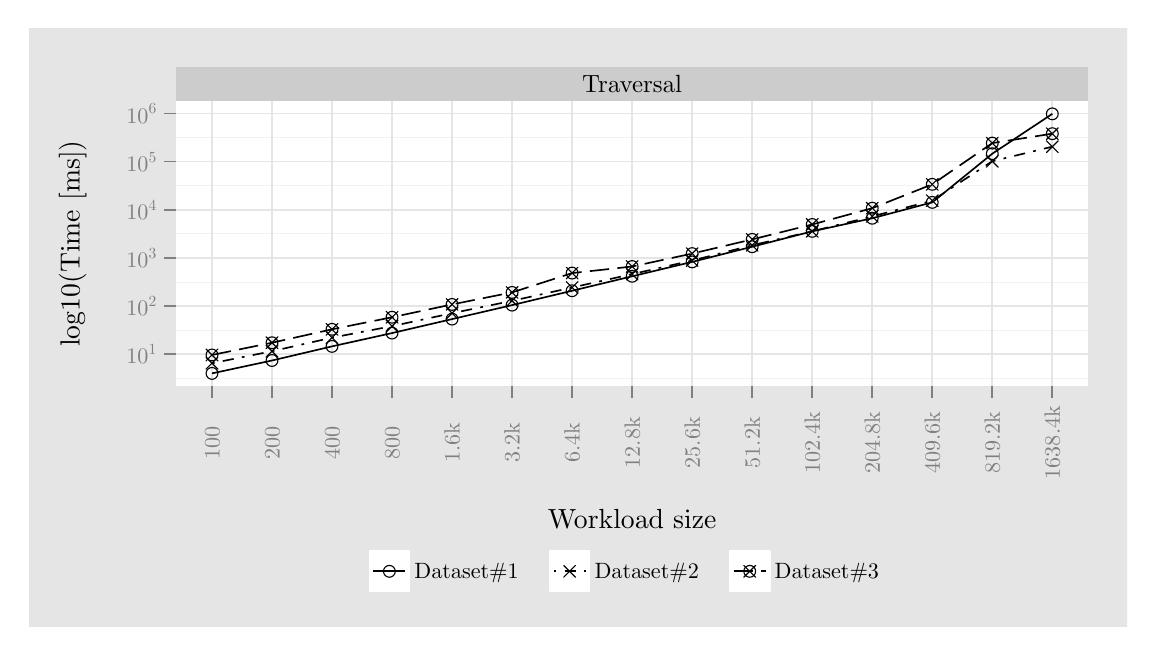
\begin{tikzpicture}[x=1pt,y=1pt]
\definecolor[named]{fillColor}{rgb}{1.00,1.00,1.00}
\path[use as bounding box,fill=fillColor,fill opacity=0.00] (0,0) rectangle (397.48,216.81);
\begin{scope}
\path[clip] (  0.00,  0.00) rectangle (397.48,216.81);
\definecolor[named]{drawColor}{rgb}{1.00,1.00,1.00}
\definecolor[named]{fillColor}{rgb}{0.90,0.90,0.90}

\path[draw=drawColor,line width= 0.6pt,line join=round,line cap=round,fill=fillColor] (  0.00,  0.00) rectangle (397.48,216.81);
\end{scope}
\begin{scope}
\path[clip] ( 53.58, 87.19) rectangle (383.26,190.36);
\definecolor[named]{fillColor}{rgb}{1.00,1.00,1.00}

\path[fill=fillColor] ( 53.58, 87.19) rectangle (383.26,190.36);
\definecolor[named]{drawColor}{rgb}{0.95,0.95,0.95}

\path[draw=drawColor,line width= 0.3pt,line join=round] ( 53.58, 90.14) --
	(383.26, 90.14);

\path[draw=drawColor,line width= 0.3pt,line join=round] ( 53.58,107.53) --
	(383.26,107.53);

\path[draw=drawColor,line width= 0.3pt,line join=round] ( 53.58,124.92) --
	(383.26,124.92);

\path[draw=drawColor,line width= 0.3pt,line join=round] ( 53.58,142.31) --
	(383.26,142.31);

\path[draw=drawColor,line width= 0.3pt,line join=round] ( 53.58,159.70) --
	(383.26,159.70);

\path[draw=drawColor,line width= 0.3pt,line join=round] ( 53.58,177.09) --
	(383.26,177.09);
\definecolor[named]{drawColor}{rgb}{0.90,0.90,0.90}

\path[draw=drawColor,line width= 0.6pt,line join=round] ( 53.58, 98.84) --
	(383.26, 98.84);

\path[draw=drawColor,line width= 0.6pt,line join=round] ( 53.58,116.23) --
	(383.26,116.23);

\path[draw=drawColor,line width= 0.6pt,line join=round] ( 53.58,133.62) --
	(383.26,133.62);

\path[draw=drawColor,line width= 0.6pt,line join=round] ( 53.58,151.01) --
	(383.26,151.01);

\path[draw=drawColor,line width= 0.6pt,line join=round] ( 53.58,168.40) --
	(383.26,168.40);

\path[draw=drawColor,line width= 0.6pt,line join=round] ( 53.58,185.79) --
	(383.26,185.79);

\path[draw=drawColor,line width= 0.6pt,line join=round] ( 66.60, 87.19) --
	( 66.60,190.36);

\path[draw=drawColor,line width= 0.6pt,line join=round] ( 88.29, 87.19) --
	( 88.29,190.36);

\path[draw=drawColor,line width= 0.6pt,line join=round] (109.97, 87.19) --
	(109.97,190.36);

\path[draw=drawColor,line width= 0.6pt,line join=round] (131.66, 87.19) --
	(131.66,190.36);

\path[draw=drawColor,line width= 0.6pt,line join=round] (153.35, 87.19) --
	(153.35,190.36);

\path[draw=drawColor,line width= 0.6pt,line join=round] (175.04, 87.19) --
	(175.04,190.36);

\path[draw=drawColor,line width= 0.6pt,line join=round] (196.73, 87.19) --
	(196.73,190.36);

\path[draw=drawColor,line width= 0.6pt,line join=round] (218.42, 87.19) --
	(218.42,190.36);

\path[draw=drawColor,line width= 0.6pt,line join=round] (240.11, 87.19) --
	(240.11,190.36);

\path[draw=drawColor,line width= 0.6pt,line join=round] (261.80, 87.19) --
	(261.80,190.36);

\path[draw=drawColor,line width= 0.6pt,line join=round] (283.49, 87.19) --
	(283.49,190.36);

\path[draw=drawColor,line width= 0.6pt,line join=round] (305.18, 87.19) --
	(305.18,190.36);

\path[draw=drawColor,line width= 0.6pt,line join=round] (326.87, 87.19) --
	(326.87,190.36);

\path[draw=drawColor,line width= 0.6pt,line join=round] (348.56, 87.19) --
	(348.56,190.36);

\path[draw=drawColor,line width= 0.6pt,line join=round] (370.25, 87.19) --
	(370.25,190.36);
\definecolor[named]{drawColor}{rgb}{0.00,0.00,0.00}

\path[draw=drawColor,line width= 0.6pt,line join=round] ( 66.60, 91.88) --
	( 88.29, 96.54) --
	(109.97,101.64) --
	(131.66,106.45) --
	(153.35,111.50) --
	(175.04,116.55) --
	(196.73,121.74) --
	(218.42,126.97) --
	(240.11,132.17) --
	(261.80,137.65) --
	(283.49,143.21) --
	(305.18,147.94) --
	(326.87,153.68) --
	(348.56,171.27) --
	(370.25,185.67);

\path[draw=drawColor,line width= 0.6pt,dash pattern=on 1pt off 3pt on 4pt off 3pt ,line join=round] ( 66.60, 95.56) --
	( 88.29, 99.89) --
	(109.97,104.79) --
	(131.66,108.95) --
	(153.35,113.63) --
	(175.04,118.10) --
	(196.73,122.91) --
	(218.42,127.76) --
	(240.11,132.66) --
	(261.80,138.19) --
	(283.49,143.23) --
	(305.18,148.61) --
	(326.87,154.30) --
	(348.56,168.54) --
	(370.25,173.81);

\path[draw=drawColor,line width= 0.6pt,dash pattern=on 7pt off 3pt ,line join=round] ( 66.60, 98.54) --
	( 88.29,102.96) --
	(109.97,107.81) --
	(131.66,112.17) --
	(153.35,116.80) --
	(175.04,121.14) --
	(196.73,128.13) --
	(218.42,130.50) --
	(240.11,135.17) --
	(261.80,140.30) --
	(283.49,145.69) --
	(305.18,151.58) --
	(326.87,160.20) --
	(348.56,175.10) --
	(370.25,178.50);

\path[draw=drawColor,line width= 0.4pt,line join=round,line cap=round] ( 66.60, 91.88) circle (  2.13);

\path[draw=drawColor,line width= 0.4pt,line join=round,line cap=round] ( 88.29, 96.54) circle (  2.13);

\path[draw=drawColor,line width= 0.4pt,line join=round,line cap=round] (109.97,101.64) circle (  2.13);

\path[draw=drawColor,line width= 0.4pt,line join=round,line cap=round] (131.66,106.45) circle (  2.13);

\path[draw=drawColor,line width= 0.4pt,line join=round,line cap=round] (153.35,111.50) circle (  2.13);

\path[draw=drawColor,line width= 0.4pt,line join=round,line cap=round] (175.04,116.55) circle (  2.13);

\path[draw=drawColor,line width= 0.4pt,line join=round,line cap=round] (196.73,121.74) circle (  2.13);

\path[draw=drawColor,line width= 0.4pt,line join=round,line cap=round] (218.42,126.97) circle (  2.13);

\path[draw=drawColor,line width= 0.4pt,line join=round,line cap=round] (240.11,132.17) circle (  2.13);

\path[draw=drawColor,line width= 0.4pt,line join=round,line cap=round] (261.80,137.65) circle (  2.13);

\path[draw=drawColor,line width= 0.4pt,line join=round,line cap=round] (283.49,143.21) circle (  2.13);

\path[draw=drawColor,line width= 0.4pt,line join=round,line cap=round] (305.18,147.94) circle (  2.13);

\path[draw=drawColor,line width= 0.4pt,line join=round,line cap=round] (326.87,153.68) circle (  2.13);

\path[draw=drawColor,line width= 0.4pt,line join=round,line cap=round] (348.56,171.27) circle (  2.13);

\path[draw=drawColor,line width= 0.4pt,line join=round,line cap=round] (370.25,185.67) circle (  2.13);

\path[draw=drawColor,line width= 0.4pt,line join=round,line cap=round] ( 64.46, 93.43) -- ( 68.73, 97.70);

\path[draw=drawColor,line width= 0.4pt,line join=round,line cap=round] ( 64.46, 97.70) -- ( 68.73, 93.43);

\path[draw=drawColor,line width= 0.4pt,line join=round,line cap=round] ( 86.15, 97.75) -- ( 90.42,102.02);

\path[draw=drawColor,line width= 0.4pt,line join=round,line cap=round] ( 86.15,102.02) -- ( 90.42, 97.75);

\path[draw=drawColor,line width= 0.4pt,line join=round,line cap=round] (107.84,102.66) -- (112.11,106.93);

\path[draw=drawColor,line width= 0.4pt,line join=round,line cap=round] (107.84,106.93) -- (112.11,102.66);

\path[draw=drawColor,line width= 0.4pt,line join=round,line cap=round] (129.53,106.81) -- (133.80,111.08);

\path[draw=drawColor,line width= 0.4pt,line join=round,line cap=round] (129.53,111.08) -- (133.80,106.81);

\path[draw=drawColor,line width= 0.4pt,line join=round,line cap=round] (151.22,111.50) -- (155.49,115.77);

\path[draw=drawColor,line width= 0.4pt,line join=round,line cap=round] (151.22,115.77) -- (155.49,111.50);

\path[draw=drawColor,line width= 0.4pt,line join=round,line cap=round] (172.91,115.96) -- (177.18,120.23);

\path[draw=drawColor,line width= 0.4pt,line join=round,line cap=round] (172.91,120.23) -- (177.18,115.96);

\path[draw=drawColor,line width= 0.4pt,line join=round,line cap=round] (194.60,120.77) -- (198.87,125.04);

\path[draw=drawColor,line width= 0.4pt,line join=round,line cap=round] (194.60,125.04) -- (198.87,120.77);

\path[draw=drawColor,line width= 0.4pt,line join=round,line cap=round] (216.29,125.62) -- (220.55,129.89);

\path[draw=drawColor,line width= 0.4pt,line join=round,line cap=round] (216.29,129.89) -- (220.55,125.62);

\path[draw=drawColor,line width= 0.4pt,line join=round,line cap=round] (237.98,130.53) -- (242.24,134.80);

\path[draw=drawColor,line width= 0.4pt,line join=round,line cap=round] (237.98,134.80) -- (242.24,130.53);

\path[draw=drawColor,line width= 0.4pt,line join=round,line cap=round] (259.67,136.06) -- (263.93,140.32);

\path[draw=drawColor,line width= 0.4pt,line join=round,line cap=round] (259.67,140.32) -- (263.93,136.06);

\path[draw=drawColor,line width= 0.4pt,line join=round,line cap=round] (281.35,141.09) -- (285.62,145.36);

\path[draw=drawColor,line width= 0.4pt,line join=round,line cap=round] (281.35,145.36) -- (285.62,141.09);

\path[draw=drawColor,line width= 0.4pt,line join=round,line cap=round] (303.04,146.48) -- (307.31,150.75);

\path[draw=drawColor,line width= 0.4pt,line join=round,line cap=round] (303.04,150.75) -- (307.31,146.48);

\path[draw=drawColor,line width= 0.4pt,line join=round,line cap=round] (324.73,152.16) -- (329.00,156.43);

\path[draw=drawColor,line width= 0.4pt,line join=round,line cap=round] (324.73,156.43) -- (329.00,152.16);

\path[draw=drawColor,line width= 0.4pt,line join=round,line cap=round] (346.42,166.40) -- (350.69,170.67);

\path[draw=drawColor,line width= 0.4pt,line join=round,line cap=round] (346.42,170.67) -- (350.69,166.40);

\path[draw=drawColor,line width= 0.4pt,line join=round,line cap=round] (368.11,171.67) -- (372.38,175.94);

\path[draw=drawColor,line width= 0.4pt,line join=round,line cap=round] (368.11,175.94) -- (372.38,171.67);

\path[draw=drawColor,line width= 0.4pt,line join=round,line cap=round] ( 66.60, 98.54) circle (  2.13);

\path[draw=drawColor,line width= 0.4pt,line join=round,line cap=round] ( 64.46, 96.40) -- ( 68.73,100.67);

\path[draw=drawColor,line width= 0.4pt,line join=round,line cap=round] ( 64.46,100.67) -- ( 68.73, 96.40);

\path[draw=drawColor,line width= 0.4pt,line join=round,line cap=round] ( 88.29,102.96) circle (  2.13);

\path[draw=drawColor,line width= 0.4pt,line join=round,line cap=round] ( 86.15,100.83) -- ( 90.42,105.10);

\path[draw=drawColor,line width= 0.4pt,line join=round,line cap=round] ( 86.15,105.10) -- ( 90.42,100.83);

\path[draw=drawColor,line width= 0.4pt,line join=round,line cap=round] (109.97,107.81) circle (  2.13);

\path[draw=drawColor,line width= 0.4pt,line join=round,line cap=round] (107.84,105.67) -- (112.11,109.94);

\path[draw=drawColor,line width= 0.4pt,line join=round,line cap=round] (107.84,109.94) -- (112.11,105.67);

\path[draw=drawColor,line width= 0.4pt,line join=round,line cap=round] (131.66,112.17) circle (  2.13);

\path[draw=drawColor,line width= 0.4pt,line join=round,line cap=round] (129.53,110.04) -- (133.80,114.30);

\path[draw=drawColor,line width= 0.4pt,line join=round,line cap=round] (129.53,114.30) -- (133.80,110.04);

\path[draw=drawColor,line width= 0.4pt,line join=round,line cap=round] (153.35,116.80) circle (  2.13);

\path[draw=drawColor,line width= 0.4pt,line join=round,line cap=round] (151.22,114.67) -- (155.49,118.94);

\path[draw=drawColor,line width= 0.4pt,line join=round,line cap=round] (151.22,118.94) -- (155.49,114.67);

\path[draw=drawColor,line width= 0.4pt,line join=round,line cap=round] (175.04,121.14) circle (  2.13);

\path[draw=drawColor,line width= 0.4pt,line join=round,line cap=round] (172.91,119.01) -- (177.18,123.28);

\path[draw=drawColor,line width= 0.4pt,line join=round,line cap=round] (172.91,123.28) -- (177.18,119.01);

\path[draw=drawColor,line width= 0.4pt,line join=round,line cap=round] (196.73,128.13) circle (  2.13);

\path[draw=drawColor,line width= 0.4pt,line join=round,line cap=round] (194.60,126.00) -- (198.87,130.27);

\path[draw=drawColor,line width= 0.4pt,line join=round,line cap=round] (194.60,130.27) -- (198.87,126.00);

\path[draw=drawColor,line width= 0.4pt,line join=round,line cap=round] (218.42,130.50) circle (  2.13);

\path[draw=drawColor,line width= 0.4pt,line join=round,line cap=round] (216.29,128.36) -- (220.55,132.63);

\path[draw=drawColor,line width= 0.4pt,line join=round,line cap=round] (216.29,132.63) -- (220.55,128.36);

\path[draw=drawColor,line width= 0.4pt,line join=round,line cap=round] (240.11,135.17) circle (  2.13);

\path[draw=drawColor,line width= 0.4pt,line join=round,line cap=round] (237.98,133.04) -- (242.24,137.30);

\path[draw=drawColor,line width= 0.4pt,line join=round,line cap=round] (237.98,137.30) -- (242.24,133.04);

\path[draw=drawColor,line width= 0.4pt,line join=round,line cap=round] (261.80,140.30) circle (  2.13);

\path[draw=drawColor,line width= 0.4pt,line join=round,line cap=round] (259.67,138.17) -- (263.93,142.43);

\path[draw=drawColor,line width= 0.4pt,line join=round,line cap=round] (259.67,142.43) -- (263.93,138.17);

\path[draw=drawColor,line width= 0.4pt,line join=round,line cap=round] (283.49,145.69) circle (  2.13);

\path[draw=drawColor,line width= 0.4pt,line join=round,line cap=round] (281.35,143.56) -- (285.62,147.83);

\path[draw=drawColor,line width= 0.4pt,line join=round,line cap=round] (281.35,147.83) -- (285.62,143.56);

\path[draw=drawColor,line width= 0.4pt,line join=round,line cap=round] (305.18,151.58) circle (  2.13);

\path[draw=drawColor,line width= 0.4pt,line join=round,line cap=round] (303.04,149.45) -- (307.31,153.71);

\path[draw=drawColor,line width= 0.4pt,line join=round,line cap=round] (303.04,153.71) -- (307.31,149.45);

\path[draw=drawColor,line width= 0.4pt,line join=round,line cap=round] (326.87,160.20) circle (  2.13);

\path[draw=drawColor,line width= 0.4pt,line join=round,line cap=round] (324.73,158.06) -- (329.00,162.33);

\path[draw=drawColor,line width= 0.4pt,line join=round,line cap=round] (324.73,162.33) -- (329.00,158.06);

\path[draw=drawColor,line width= 0.4pt,line join=round,line cap=round] (348.56,175.10) circle (  2.13);

\path[draw=drawColor,line width= 0.4pt,line join=round,line cap=round] (346.42,172.97) -- (350.69,177.23);

\path[draw=drawColor,line width= 0.4pt,line join=round,line cap=round] (346.42,177.23) -- (350.69,172.97);

\path[draw=drawColor,line width= 0.4pt,line join=round,line cap=round] (370.25,178.50) circle (  2.13);

\path[draw=drawColor,line width= 0.4pt,line join=round,line cap=round] (368.11,176.37) -- (372.38,180.63);

\path[draw=drawColor,line width= 0.4pt,line join=round,line cap=round] (368.11,180.63) -- (372.38,176.37);
\end{scope}
\begin{scope}
\path[clip] (  0.00,  0.00) rectangle (397.48,216.81);
\definecolor[named]{fillColor}{rgb}{0.80,0.80,0.80}

\path[fill=fillColor] ( 53.58,190.36) rectangle (383.26,202.58);
\definecolor[named]{drawColor}{rgb}{0.00,0.00,0.00}

\node[text=drawColor,anchor=base,inner sep=0pt, outer sep=0pt, scale=  0.90] at (218.42,193.37) {Traversal};
\end{scope}
\begin{scope}
\path[clip] (  0.00,  0.00) rectangle (397.48,216.81);
\definecolor[named]{drawColor}{rgb}{0.50,0.50,0.50}

\node[text=drawColor,anchor=base west,inner sep=0pt, outer sep=0pt, scale=  0.80] at ( 35.67, 95.40) {10};

\node[text=drawColor,anchor=base west,inner sep=0pt, outer sep=0pt, scale=  0.56] at ( 43.67, 98.67) {1};

\node[text=drawColor,anchor=base west,inner sep=0pt, outer sep=0pt, scale=  0.80] at ( 35.67,112.79) {10};

\node[text=drawColor,anchor=base west,inner sep=0pt, outer sep=0pt, scale=  0.56] at ( 43.67,116.07) {2};

\node[text=drawColor,anchor=base west,inner sep=0pt, outer sep=0pt, scale=  0.80] at ( 35.67,130.18) {10};

\node[text=drawColor,anchor=base west,inner sep=0pt, outer sep=0pt, scale=  0.56] at ( 43.67,133.46) {3};

\node[text=drawColor,anchor=base west,inner sep=0pt, outer sep=0pt, scale=  0.80] at ( 35.67,147.57) {10};

\node[text=drawColor,anchor=base west,inner sep=0pt, outer sep=0pt, scale=  0.56] at ( 43.67,150.85) {4};

\node[text=drawColor,anchor=base west,inner sep=0pt, outer sep=0pt, scale=  0.80] at ( 35.67,164.96) {10};

\node[text=drawColor,anchor=base west,inner sep=0pt, outer sep=0pt, scale=  0.56] at ( 43.67,168.24) {5};

\node[text=drawColor,anchor=base west,inner sep=0pt, outer sep=0pt, scale=  0.80] at ( 35.67,182.35) {10};

\node[text=drawColor,anchor=base west,inner sep=0pt, outer sep=0pt, scale=  0.56] at ( 43.67,185.63) {6};
\end{scope}
\begin{scope}
\path[clip] (  0.00,  0.00) rectangle (397.48,216.81);
\definecolor[named]{drawColor}{rgb}{0.50,0.50,0.50}

\path[draw=drawColor,line width= 0.6pt,line join=round] ( 49.31, 98.84) --
	( 53.58, 98.84);

\path[draw=drawColor,line width= 0.6pt,line join=round] ( 49.31,116.23) --
	( 53.58,116.23);

\path[draw=drawColor,line width= 0.6pt,line join=round] ( 49.31,133.62) --
	( 53.58,133.62);

\path[draw=drawColor,line width= 0.6pt,line join=round] ( 49.31,151.01) --
	( 53.58,151.01);

\path[draw=drawColor,line width= 0.6pt,line join=round] ( 49.31,168.40) --
	( 53.58,168.40);

\path[draw=drawColor,line width= 0.6pt,line join=round] ( 49.31,185.79) --
	( 53.58,185.79);
\end{scope}
\begin{scope}
\path[clip] (  0.00,  0.00) rectangle (397.48,216.81);
\definecolor[named]{drawColor}{rgb}{0.50,0.50,0.50}

\path[draw=drawColor,line width= 0.6pt,line join=round] ( 66.60, 82.92) --
	( 66.60, 87.19);

\path[draw=drawColor,line width= 0.6pt,line join=round] ( 88.29, 82.92) --
	( 88.29, 87.19);

\path[draw=drawColor,line width= 0.6pt,line join=round] (109.97, 82.92) --
	(109.97, 87.19);

\path[draw=drawColor,line width= 0.6pt,line join=round] (131.66, 82.92) --
	(131.66, 87.19);

\path[draw=drawColor,line width= 0.6pt,line join=round] (153.35, 82.92) --
	(153.35, 87.19);

\path[draw=drawColor,line width= 0.6pt,line join=round] (175.04, 82.92) --
	(175.04, 87.19);

\path[draw=drawColor,line width= 0.6pt,line join=round] (196.73, 82.92) --
	(196.73, 87.19);

\path[draw=drawColor,line width= 0.6pt,line join=round] (218.42, 82.92) --
	(218.42, 87.19);

\path[draw=drawColor,line width= 0.6pt,line join=round] (240.11, 82.92) --
	(240.11, 87.19);

\path[draw=drawColor,line width= 0.6pt,line join=round] (261.80, 82.92) --
	(261.80, 87.19);

\path[draw=drawColor,line width= 0.6pt,line join=round] (283.49, 82.92) --
	(283.49, 87.19);

\path[draw=drawColor,line width= 0.6pt,line join=round] (305.18, 82.92) --
	(305.18, 87.19);

\path[draw=drawColor,line width= 0.6pt,line join=round] (326.87, 82.92) --
	(326.87, 87.19);

\path[draw=drawColor,line width= 0.6pt,line join=round] (348.56, 82.92) --
	(348.56, 87.19);

\path[draw=drawColor,line width= 0.6pt,line join=round] (370.25, 82.92) --
	(370.25, 87.19);
\end{scope}
\begin{scope}
\path[clip] (  0.00,  0.00) rectangle (397.48,216.81);
\definecolor[named]{drawColor}{rgb}{0.50,0.50,0.50}

\node[text=drawColor,rotate= 90.00,anchor=base,inner sep=0pt, outer sep=0pt, scale=  0.80] at ( 69.35, 66.85) {100};

\node[text=drawColor,rotate= 90.00,anchor=base,inner sep=0pt, outer sep=0pt, scale=  0.80] at ( 91.04, 66.85) {200};

\node[text=drawColor,rotate= 90.00,anchor=base,inner sep=0pt, outer sep=0pt, scale=  0.80] at (112.73, 66.85) {400};

\node[text=drawColor,rotate= 90.00,anchor=base,inner sep=0pt, outer sep=0pt, scale=  0.80] at (134.42, 66.85) {800};

\node[text=drawColor,rotate= 90.00,anchor=base,inner sep=0pt, outer sep=0pt, scale=  0.80] at (156.11, 66.85) {1.6k};

\node[text=drawColor,rotate= 90.00,anchor=base,inner sep=0pt, outer sep=0pt, scale=  0.80] at (177.80, 66.85) {3.2k};

\node[text=drawColor,rotate= 90.00,anchor=base,inner sep=0pt, outer sep=0pt, scale=  0.80] at (199.49, 66.85) {6.4k};

\node[text=drawColor,rotate= 90.00,anchor=base,inner sep=0pt, outer sep=0pt, scale=  0.80] at (221.18, 66.85) {12.8k};

\node[text=drawColor,rotate= 90.00,anchor=base,inner sep=0pt, outer sep=0pt, scale=  0.80] at (242.86, 66.85) {25.6k};

\node[text=drawColor,rotate= 90.00,anchor=base,inner sep=0pt, outer sep=0pt, scale=  0.80] at (264.55, 66.85) {51.2k};

\node[text=drawColor,rotate= 90.00,anchor=base,inner sep=0pt, outer sep=0pt, scale=  0.80] at (286.24, 66.85) {102.4k};

\node[text=drawColor,rotate= 90.00,anchor=base,inner sep=0pt, outer sep=0pt, scale=  0.80] at (307.93, 66.85) {204.8k};

\node[text=drawColor,rotate= 90.00,anchor=base,inner sep=0pt, outer sep=0pt, scale=  0.80] at (329.62, 66.85) {409.6k};

\node[text=drawColor,rotate= 90.00,anchor=base,inner sep=0pt, outer sep=0pt, scale=  0.80] at (351.31, 66.85) {819.2k};

\node[text=drawColor,rotate= 90.00,anchor=base,inner sep=0pt, outer sep=0pt, scale=  0.80] at (373.00, 66.85) {1638.4k};
\end{scope}
\begin{scope}
\path[clip] (  0.00,  0.00) rectangle (397.48,216.81);
\definecolor[named]{drawColor}{rgb}{0.00,0.00,0.00}

\node[text=drawColor,anchor=base,inner sep=0pt, outer sep=0pt, scale=  1.00] at (218.42, 35.91) {Workload size};
\end{scope}
\begin{scope}
\path[clip] (  0.00,  0.00) rectangle (397.48,216.81);
\definecolor[named]{drawColor}{rgb}{0.00,0.00,0.00}

\node[text=drawColor,rotate= 90.00,anchor=base,inner sep=0pt, outer sep=0pt, scale=  1.00] at ( 18.80,138.77) {log10(Time [ms])};
\end{scope}
\begin{scope}
\path[clip] (  0.00,  0.00) rectangle (397.48,216.81);
\definecolor[named]{fillColor}{rgb}{0.90,0.90,0.90}

\path[fill=fillColor] (115.60,  8.87) rectangle (321.24, 31.86);
\end{scope}
\begin{scope}
\path[clip] (  0.00,  0.00) rectangle (397.48,216.81);
\definecolor[named]{drawColor}{rgb}{1.00,1.00,1.00}
\definecolor[named]{fillColor}{rgb}{1.00,1.00,1.00}

\path[draw=drawColor,line width= 0.6pt,line join=round,line cap=round,fill=fillColor] (123.48, 13.14) rectangle (137.93, 27.59);
\end{scope}
\begin{scope}
\path[clip] (  0.00,  0.00) rectangle (397.48,216.81);
\definecolor[named]{drawColor}{rgb}{0.00,0.00,0.00}

\path[draw=drawColor,line width= 0.6pt,line join=round] (124.92, 20.36) -- (136.49, 20.36);
\end{scope}
\begin{scope}
\path[clip] (  0.00,  0.00) rectangle (397.48,216.81);
\definecolor[named]{drawColor}{rgb}{0.00,0.00,0.00}

\path[draw=drawColor,line width= 0.4pt,line join=round,line cap=round] (130.70, 20.36) circle (  2.13);
\end{scope}
\begin{scope}
\path[clip] (  0.00,  0.00) rectangle (397.48,216.81);
\definecolor[named]{drawColor}{rgb}{1.00,1.00,1.00}
\definecolor[named]{fillColor}{rgb}{1.00,1.00,1.00}

\path[draw=drawColor,line width= 0.6pt,line join=round,line cap=round,fill=fillColor] (188.58, 13.14) rectangle (203.03, 27.59);
\end{scope}
\begin{scope}
\path[clip] (  0.00,  0.00) rectangle (397.48,216.81);
\definecolor[named]{drawColor}{rgb}{0.00,0.00,0.00}

\path[draw=drawColor,line width= 0.6pt,dash pattern=on 1pt off 3pt on 4pt off 3pt ,line join=round] (190.03, 20.36) -- (201.59, 20.36);
\end{scope}
\begin{scope}
\path[clip] (  0.00,  0.00) rectangle (397.48,216.81);
\definecolor[named]{drawColor}{rgb}{0.00,0.00,0.00}

\path[draw=drawColor,line width= 0.4pt,line join=round,line cap=round] (193.67, 18.23) -- (197.94, 22.50);

\path[draw=drawColor,line width= 0.4pt,line join=round,line cap=round] (193.67, 22.50) -- (197.94, 18.23);
\end{scope}
\begin{scope}
\path[clip] (  0.00,  0.00) rectangle (397.48,216.81);
\definecolor[named]{drawColor}{rgb}{1.00,1.00,1.00}
\definecolor[named]{fillColor}{rgb}{1.00,1.00,1.00}

\path[draw=drawColor,line width= 0.6pt,line join=round,line cap=round,fill=fillColor] (253.68, 13.14) rectangle (268.14, 27.59);
\end{scope}
\begin{scope}
\path[clip] (  0.00,  0.00) rectangle (397.48,216.81);
\definecolor[named]{drawColor}{rgb}{0.00,0.00,0.00}

\path[draw=drawColor,line width= 0.6pt,dash pattern=on 7pt off 3pt ,line join=round] (255.13, 20.36) -- (266.69, 20.36);
\end{scope}
\begin{scope}
\path[clip] (  0.00,  0.00) rectangle (397.48,216.81);
\definecolor[named]{drawColor}{rgb}{0.00,0.00,0.00}

\path[draw=drawColor,line width= 0.4pt,line join=round,line cap=round] (260.91, 20.36) circle (  2.13);

\path[draw=drawColor,line width= 0.4pt,line join=round,line cap=round] (258.77, 18.23) -- (263.04, 22.50);

\path[draw=drawColor,line width= 0.4pt,line join=round,line cap=round] (258.77, 22.50) -- (263.04, 18.23);
\end{scope}
\begin{scope}
\path[clip] (  0.00,  0.00) rectangle (397.48,216.81);
\definecolor[named]{drawColor}{rgb}{0.00,0.00,0.00}

\node[text=drawColor,anchor=base west,inner sep=0pt, outer sep=0pt, scale=  0.80] at (139.74, 17.61) {Dataset\#1 $\;\;\;$};
\end{scope}
\begin{scope}
\path[clip] (  0.00,  0.00) rectangle (397.48,216.81);
\definecolor[named]{drawColor}{rgb}{0.00,0.00,0.00}

\node[text=drawColor,anchor=base west,inner sep=0pt, outer sep=0pt, scale=  0.80] at (204.84, 17.61) {Dataset\#2 $\;\;\;$};
\end{scope}
\begin{scope}
\path[clip] (  0.00,  0.00) rectangle (397.48,216.81);
\definecolor[named]{drawColor}{rgb}{0.00,0.00,0.00}

\node[text=drawColor,anchor=base west,inner sep=0pt, outer sep=0pt, scale=  0.80] at (269.94, 17.61) {Dataset\#3 $\;\;\;$};
\end{scope}
\end{tikzpicture}

 }
 \caption[Impact of structure on traversal query phase]{Impact of structure on traversal query phase.}
 \label{fig:experimentation:performance:search:processing-phases-traversal-levels}
\end{figure}

\begin{figure}
 \centering
 \framebox[\textwidth]{%
% Created by tikzDevice version 0.6.2-92-0ad2792 on 2013-03-23 22:56:34
% !TEX encoding = UTF-8 Unicode
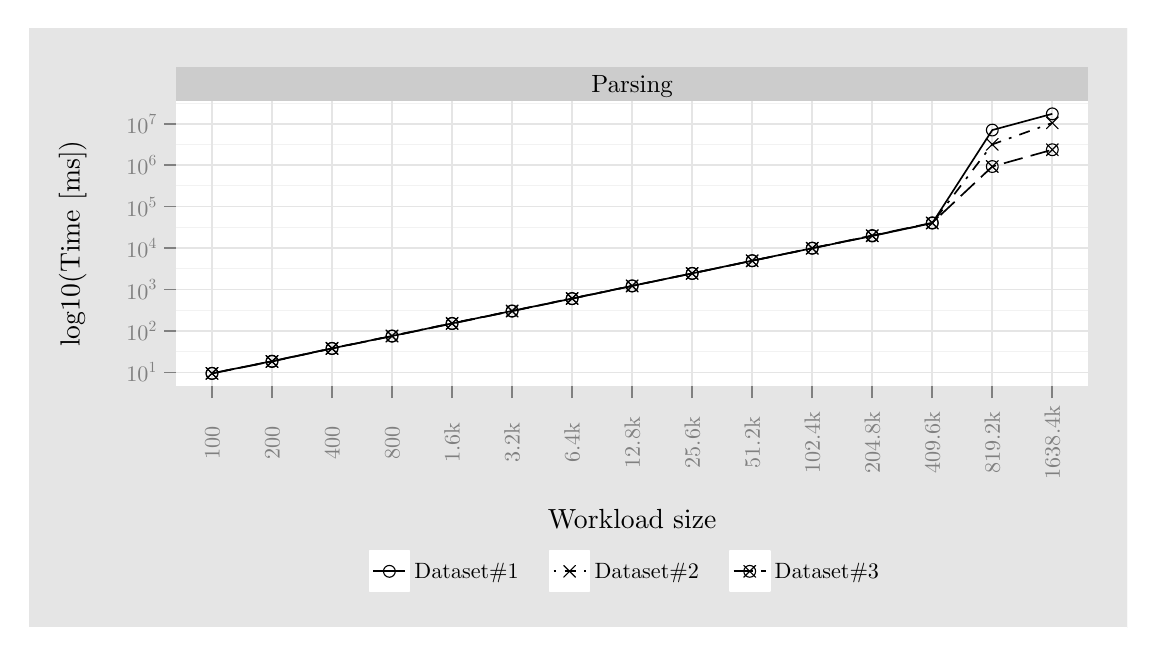
\begin{tikzpicture}[x=1pt,y=1pt]
\definecolor[named]{fillColor}{rgb}{1.00,1.00,1.00}
\path[use as bounding box,fill=fillColor,fill opacity=0.00] (0,0) rectangle (397.48,216.81);
\begin{scope}
\path[clip] (  0.00,  0.00) rectangle (397.48,216.81);
\definecolor[named]{drawColor}{rgb}{1.00,1.00,1.00}
\definecolor[named]{fillColor}{rgb}{0.90,0.90,0.90}

\path[draw=drawColor,line width= 0.6pt,line join=round,line cap=round,fill=fillColor] (  0.00,  0.00) rectangle (397.48,216.81);
\end{scope}
\begin{scope}
\path[clip] ( 53.58, 87.19) rectangle (383.26,190.36);
\definecolor[named]{fillColor}{rgb}{1.00,1.00,1.00}

\path[fill=fillColor] ( 53.58, 87.19) rectangle (383.26,190.36);
\definecolor[named]{drawColor}{rgb}{0.95,0.95,0.95}

\path[draw=drawColor,line width= 0.3pt,line join=round] ( 53.58, 99.73) --
	(383.26, 99.73);

\path[draw=drawColor,line width= 0.3pt,line join=round] ( 53.58,114.70) --
	(383.26,114.70);

\path[draw=drawColor,line width= 0.3pt,line join=round] ( 53.58,129.68) --
	(383.26,129.68);

\path[draw=drawColor,line width= 0.3pt,line join=round] ( 53.58,144.66) --
	(383.26,144.66);

\path[draw=drawColor,line width= 0.3pt,line join=round] ( 53.58,159.63) --
	(383.26,159.63);

\path[draw=drawColor,line width= 0.3pt,line join=round] ( 53.58,174.61) --
	(383.26,174.61);

\path[draw=drawColor,line width= 0.3pt,line join=round] ( 53.58,189.58) --
	(383.26,189.58);
\definecolor[named]{drawColor}{rgb}{0.90,0.90,0.90}

\path[draw=drawColor,line width= 0.6pt,line join=round] ( 53.58, 92.24) --
	(383.26, 92.24);

\path[draw=drawColor,line width= 0.6pt,line join=round] ( 53.58,107.22) --
	(383.26,107.22);

\path[draw=drawColor,line width= 0.6pt,line join=round] ( 53.58,122.19) --
	(383.26,122.19);

\path[draw=drawColor,line width= 0.6pt,line join=round] ( 53.58,137.17) --
	(383.26,137.17);

\path[draw=drawColor,line width= 0.6pt,line join=round] ( 53.58,152.14) --
	(383.26,152.14);

\path[draw=drawColor,line width= 0.6pt,line join=round] ( 53.58,167.12) --
	(383.26,167.12);

\path[draw=drawColor,line width= 0.6pt,line join=round] ( 53.58,182.09) --
	(383.26,182.09);

\path[draw=drawColor,line width= 0.6pt,line join=round] ( 66.60, 87.19) --
	( 66.60,190.36);

\path[draw=drawColor,line width= 0.6pt,line join=round] ( 88.29, 87.19) --
	( 88.29,190.36);

\path[draw=drawColor,line width= 0.6pt,line join=round] (109.97, 87.19) --
	(109.97,190.36);

\path[draw=drawColor,line width= 0.6pt,line join=round] (131.66, 87.19) --
	(131.66,190.36);

\path[draw=drawColor,line width= 0.6pt,line join=round] (153.35, 87.19) --
	(153.35,190.36);

\path[draw=drawColor,line width= 0.6pt,line join=round] (175.04, 87.19) --
	(175.04,190.36);

\path[draw=drawColor,line width= 0.6pt,line join=round] (196.73, 87.19) --
	(196.73,190.36);

\path[draw=drawColor,line width= 0.6pt,line join=round] (218.42, 87.19) --
	(218.42,190.36);

\path[draw=drawColor,line width= 0.6pt,line join=round] (240.11, 87.19) --
	(240.11,190.36);

\path[draw=drawColor,line width= 0.6pt,line join=round] (261.80, 87.19) --
	(261.80,190.36);

\path[draw=drawColor,line width= 0.6pt,line join=round] (283.49, 87.19) --
	(283.49,190.36);

\path[draw=drawColor,line width= 0.6pt,line join=round] (305.18, 87.19) --
	(305.18,190.36);

\path[draw=drawColor,line width= 0.6pt,line join=round] (326.87, 87.19) --
	(326.87,190.36);

\path[draw=drawColor,line width= 0.6pt,line join=round] (348.56, 87.19) --
	(348.56,190.36);

\path[draw=drawColor,line width= 0.6pt,line join=round] (370.25, 87.19) --
	(370.25,190.36);
\definecolor[named]{drawColor}{rgb}{0.00,0.00,0.00}

\path[draw=drawColor,line width= 0.6pt,line join=round] ( 66.60, 91.90) --
	( 88.29, 96.31) --
	(109.97,100.92) --
	(131.66,105.40) --
	(153.35,109.96) --
	(175.04,114.45) --
	(196.73,118.90) --
	(218.42,123.50) --
	(240.11,128.03) --
	(261.80,132.61) --
	(283.49,137.11) --
	(305.18,141.53) --
	(326.87,146.18) --
	(348.56,179.81) --
	(370.25,185.67);

\path[draw=drawColor,line width= 0.6pt,dash pattern=on 1pt off 3pt on 4pt off 3pt ,line join=round] ( 66.60, 91.92) --
	( 88.29, 96.24) --
	(109.97,100.96) --
	(131.66,105.43) --
	(153.35,110.01) --
	(175.04,114.46) --
	(196.73,119.01) --
	(218.42,123.52) --
	(240.11,128.04) --
	(261.80,132.55) --
	(283.49,137.08) --
	(305.18,141.60) --
	(326.87,146.18) --
	(348.56,174.62) --
	(370.25,182.39);

\path[draw=drawColor,line width= 0.6pt,dash pattern=on 7pt off 3pt ,line join=round] ( 66.60, 91.88) --
	( 88.29, 96.18) --
	(109.97,100.87) --
	(131.66,105.34) --
	(153.35,109.88) --
	(175.04,114.38) --
	(196.73,118.90) --
	(218.42,123.48) --
	(240.11,127.99) --
	(261.80,132.58) --
	(283.49,137.14) --
	(305.18,141.69) --
	(326.87,146.30) --
	(348.56,166.63) --
	(370.25,172.70);

\path[draw=drawColor,line width= 0.4pt,line join=round,line cap=round] ( 66.60, 91.90) circle (  2.13);

\path[draw=drawColor,line width= 0.4pt,line join=round,line cap=round] ( 88.29, 96.31) circle (  2.13);

\path[draw=drawColor,line width= 0.4pt,line join=round,line cap=round] (109.97,100.92) circle (  2.13);

\path[draw=drawColor,line width= 0.4pt,line join=round,line cap=round] (131.66,105.40) circle (  2.13);

\path[draw=drawColor,line width= 0.4pt,line join=round,line cap=round] (153.35,109.96) circle (  2.13);

\path[draw=drawColor,line width= 0.4pt,line join=round,line cap=round] (175.04,114.45) circle (  2.13);

\path[draw=drawColor,line width= 0.4pt,line join=round,line cap=round] (196.73,118.90) circle (  2.13);

\path[draw=drawColor,line width= 0.4pt,line join=round,line cap=round] (218.42,123.50) circle (  2.13);

\path[draw=drawColor,line width= 0.4pt,line join=round,line cap=round] (240.11,128.03) circle (  2.13);

\path[draw=drawColor,line width= 0.4pt,line join=round,line cap=round] (261.80,132.61) circle (  2.13);

\path[draw=drawColor,line width= 0.4pt,line join=round,line cap=round] (283.49,137.11) circle (  2.13);

\path[draw=drawColor,line width= 0.4pt,line join=round,line cap=round] (305.18,141.53) circle (  2.13);

\path[draw=drawColor,line width= 0.4pt,line join=round,line cap=round] (326.87,146.18) circle (  2.13);

\path[draw=drawColor,line width= 0.4pt,line join=round,line cap=round] (348.56,179.81) circle (  2.13);

\path[draw=drawColor,line width= 0.4pt,line join=round,line cap=round] (370.25,185.67) circle (  2.13);

\path[draw=drawColor,line width= 0.4pt,line join=round,line cap=round] ( 64.46, 89.78) -- ( 68.73, 94.05);

\path[draw=drawColor,line width= 0.4pt,line join=round,line cap=round] ( 64.46, 94.05) -- ( 68.73, 89.78);

\path[draw=drawColor,line width= 0.4pt,line join=round,line cap=round] ( 86.15, 94.11) -- ( 90.42, 98.38);

\path[draw=drawColor,line width= 0.4pt,line join=round,line cap=round] ( 86.15, 98.38) -- ( 90.42, 94.11);

\path[draw=drawColor,line width= 0.4pt,line join=round,line cap=round] (107.84, 98.83) -- (112.11,103.10);

\path[draw=drawColor,line width= 0.4pt,line join=round,line cap=round] (107.84,103.10) -- (112.11, 98.83);

\path[draw=drawColor,line width= 0.4pt,line join=round,line cap=round] (129.53,103.30) -- (133.80,107.56);

\path[draw=drawColor,line width= 0.4pt,line join=round,line cap=round] (129.53,107.56) -- (133.80,103.30);

\path[draw=drawColor,line width= 0.4pt,line join=round,line cap=round] (151.22,107.88) -- (155.49,112.14);

\path[draw=drawColor,line width= 0.4pt,line join=round,line cap=round] (151.22,112.14) -- (155.49,107.88);

\path[draw=drawColor,line width= 0.4pt,line join=round,line cap=round] (172.91,112.32) -- (177.18,116.59);

\path[draw=drawColor,line width= 0.4pt,line join=round,line cap=round] (172.91,116.59) -- (177.18,112.32);

\path[draw=drawColor,line width= 0.4pt,line join=round,line cap=round] (194.60,116.87) -- (198.87,121.14);

\path[draw=drawColor,line width= 0.4pt,line join=round,line cap=round] (194.60,121.14) -- (198.87,116.87);

\path[draw=drawColor,line width= 0.4pt,line join=round,line cap=round] (216.29,121.39) -- (220.55,125.66);

\path[draw=drawColor,line width= 0.4pt,line join=round,line cap=round] (216.29,125.66) -- (220.55,121.39);

\path[draw=drawColor,line width= 0.4pt,line join=round,line cap=round] (237.98,125.90) -- (242.24,130.17);

\path[draw=drawColor,line width= 0.4pt,line join=round,line cap=round] (237.98,130.17) -- (242.24,125.90);

\path[draw=drawColor,line width= 0.4pt,line join=round,line cap=round] (259.67,130.41) -- (263.93,134.68);

\path[draw=drawColor,line width= 0.4pt,line join=round,line cap=round] (259.67,134.68) -- (263.93,130.41);

\path[draw=drawColor,line width= 0.4pt,line join=round,line cap=round] (281.35,134.95) -- (285.62,139.21);

\path[draw=drawColor,line width= 0.4pt,line join=round,line cap=round] (281.35,139.21) -- (285.62,134.95);

\path[draw=drawColor,line width= 0.4pt,line join=round,line cap=round] (303.04,139.46) -- (307.31,143.73);

\path[draw=drawColor,line width= 0.4pt,line join=round,line cap=round] (303.04,143.73) -- (307.31,139.46);

\path[draw=drawColor,line width= 0.4pt,line join=round,line cap=round] (324.73,144.04) -- (329.00,148.31);

\path[draw=drawColor,line width= 0.4pt,line join=round,line cap=round] (324.73,148.31) -- (329.00,144.04);

\path[draw=drawColor,line width= 0.4pt,line join=round,line cap=round] (346.42,172.48) -- (350.69,176.75);

\path[draw=drawColor,line width= 0.4pt,line join=round,line cap=round] (346.42,176.75) -- (350.69,172.48);

\path[draw=drawColor,line width= 0.4pt,line join=round,line cap=round] (368.11,180.26) -- (372.38,184.52);

\path[draw=drawColor,line width= 0.4pt,line join=round,line cap=round] (368.11,184.52) -- (372.38,180.26);

\path[draw=drawColor,line width= 0.4pt,line join=round,line cap=round] ( 66.60, 91.88) circle (  2.13);

\path[draw=drawColor,line width= 0.4pt,line join=round,line cap=round] ( 64.46, 89.74) -- ( 68.73, 94.01);

\path[draw=drawColor,line width= 0.4pt,line join=round,line cap=round] ( 64.46, 94.01) -- ( 68.73, 89.74);

\path[draw=drawColor,line width= 0.4pt,line join=round,line cap=round] ( 88.29, 96.18) circle (  2.13);

\path[draw=drawColor,line width= 0.4pt,line join=round,line cap=round] ( 86.15, 94.05) -- ( 90.42, 98.31);

\path[draw=drawColor,line width= 0.4pt,line join=round,line cap=round] ( 86.15, 98.31) -- ( 90.42, 94.05);

\path[draw=drawColor,line width= 0.4pt,line join=round,line cap=round] (109.97,100.87) circle (  2.13);

\path[draw=drawColor,line width= 0.4pt,line join=round,line cap=round] (107.84, 98.73) -- (112.11,103.00);

\path[draw=drawColor,line width= 0.4pt,line join=round,line cap=round] (107.84,103.00) -- (112.11, 98.73);

\path[draw=drawColor,line width= 0.4pt,line join=round,line cap=round] (131.66,105.34) circle (  2.13);

\path[draw=drawColor,line width= 0.4pt,line join=round,line cap=round] (129.53,103.20) -- (133.80,107.47);

\path[draw=drawColor,line width= 0.4pt,line join=round,line cap=round] (129.53,107.47) -- (133.80,103.20);

\path[draw=drawColor,line width= 0.4pt,line join=round,line cap=round] (153.35,109.88) circle (  2.13);

\path[draw=drawColor,line width= 0.4pt,line join=round,line cap=round] (151.22,107.75) -- (155.49,112.02);

\path[draw=drawColor,line width= 0.4pt,line join=round,line cap=round] (151.22,112.02) -- (155.49,107.75);

\path[draw=drawColor,line width= 0.4pt,line join=round,line cap=round] (175.04,114.38) circle (  2.13);

\path[draw=drawColor,line width= 0.4pt,line join=round,line cap=round] (172.91,112.24) -- (177.18,116.51);

\path[draw=drawColor,line width= 0.4pt,line join=round,line cap=round] (172.91,116.51) -- (177.18,112.24);

\path[draw=drawColor,line width= 0.4pt,line join=round,line cap=round] (196.73,118.90) circle (  2.13);

\path[draw=drawColor,line width= 0.4pt,line join=round,line cap=round] (194.60,116.76) -- (198.87,121.03);

\path[draw=drawColor,line width= 0.4pt,line join=round,line cap=round] (194.60,121.03) -- (198.87,116.76);

\path[draw=drawColor,line width= 0.4pt,line join=round,line cap=round] (218.42,123.48) circle (  2.13);

\path[draw=drawColor,line width= 0.4pt,line join=round,line cap=round] (216.29,121.34) -- (220.55,125.61);

\path[draw=drawColor,line width= 0.4pt,line join=round,line cap=round] (216.29,125.61) -- (220.55,121.34);

\path[draw=drawColor,line width= 0.4pt,line join=round,line cap=round] (240.11,127.99) circle (  2.13);

\path[draw=drawColor,line width= 0.4pt,line join=round,line cap=round] (237.98,125.86) -- (242.24,130.13);

\path[draw=drawColor,line width= 0.4pt,line join=round,line cap=round] (237.98,130.13) -- (242.24,125.86);

\path[draw=drawColor,line width= 0.4pt,line join=round,line cap=round] (261.80,132.58) circle (  2.13);

\path[draw=drawColor,line width= 0.4pt,line join=round,line cap=round] (259.67,130.44) -- (263.93,134.71);

\path[draw=drawColor,line width= 0.4pt,line join=round,line cap=round] (259.67,134.71) -- (263.93,130.44);

\path[draw=drawColor,line width= 0.4pt,line join=round,line cap=round] (283.49,137.14) circle (  2.13);

\path[draw=drawColor,line width= 0.4pt,line join=round,line cap=round] (281.35,135.01) -- (285.62,139.27);

\path[draw=drawColor,line width= 0.4pt,line join=round,line cap=round] (281.35,139.27) -- (285.62,135.01);

\path[draw=drawColor,line width= 0.4pt,line join=round,line cap=round] (305.18,141.69) circle (  2.13);

\path[draw=drawColor,line width= 0.4pt,line join=round,line cap=round] (303.04,139.56) -- (307.31,143.82);

\path[draw=drawColor,line width= 0.4pt,line join=round,line cap=round] (303.04,143.82) -- (307.31,139.56);

\path[draw=drawColor,line width= 0.4pt,line join=round,line cap=round] (326.87,146.30) circle (  2.13);

\path[draw=drawColor,line width= 0.4pt,line join=round,line cap=round] (324.73,144.16) -- (329.00,148.43);

\path[draw=drawColor,line width= 0.4pt,line join=round,line cap=round] (324.73,148.43) -- (329.00,144.16);

\path[draw=drawColor,line width= 0.4pt,line join=round,line cap=round] (348.56,166.63) circle (  2.13);

\path[draw=drawColor,line width= 0.4pt,line join=round,line cap=round] (346.42,164.49) -- (350.69,168.76);

\path[draw=drawColor,line width= 0.4pt,line join=round,line cap=round] (346.42,168.76) -- (350.69,164.49);

\path[draw=drawColor,line width= 0.4pt,line join=round,line cap=round] (370.25,172.70) circle (  2.13);

\path[draw=drawColor,line width= 0.4pt,line join=round,line cap=round] (368.11,170.57) -- (372.38,174.84);

\path[draw=drawColor,line width= 0.4pt,line join=round,line cap=round] (368.11,174.84) -- (372.38,170.57);
\end{scope}
\begin{scope}
\path[clip] (  0.00,  0.00) rectangle (397.48,216.81);
\definecolor[named]{fillColor}{rgb}{0.80,0.80,0.80}

\path[fill=fillColor] ( 53.58,190.36) rectangle (383.26,202.58);
\definecolor[named]{drawColor}{rgb}{0.00,0.00,0.00}

\node[text=drawColor,anchor=base,inner sep=0pt, outer sep=0pt, scale=  0.90] at (218.42,193.37) {Parsing};
\end{scope}
\begin{scope}
\path[clip] (  0.00,  0.00) rectangle (397.48,216.81);
\definecolor[named]{drawColor}{rgb}{0.50,0.50,0.50}

\node[text=drawColor,anchor=base west,inner sep=0pt, outer sep=0pt, scale=  0.80] at ( 35.67, 88.81) {10};

\node[text=drawColor,anchor=base west,inner sep=0pt, outer sep=0pt, scale=  0.56] at ( 43.67, 92.08) {1};

\node[text=drawColor,anchor=base west,inner sep=0pt, outer sep=0pt, scale=  0.80] at ( 35.67,103.78) {10};

\node[text=drawColor,anchor=base west,inner sep=0pt, outer sep=0pt, scale=  0.56] at ( 43.67,107.05) {2};

\node[text=drawColor,anchor=base west,inner sep=0pt, outer sep=0pt, scale=  0.80] at ( 35.67,118.76) {10};

\node[text=drawColor,anchor=base west,inner sep=0pt, outer sep=0pt, scale=  0.56] at ( 43.67,122.03) {3};

\node[text=drawColor,anchor=base west,inner sep=0pt, outer sep=0pt, scale=  0.80] at ( 35.67,133.74) {10};

\node[text=drawColor,anchor=base west,inner sep=0pt, outer sep=0pt, scale=  0.56] at ( 43.67,137.01) {4};

\node[text=drawColor,anchor=base west,inner sep=0pt, outer sep=0pt, scale=  0.80] at ( 35.67,148.71) {10};

\node[text=drawColor,anchor=base west,inner sep=0pt, outer sep=0pt, scale=  0.56] at ( 43.67,151.98) {5};

\node[text=drawColor,anchor=base west,inner sep=0pt, outer sep=0pt, scale=  0.80] at ( 35.67,163.69) {10};

\node[text=drawColor,anchor=base west,inner sep=0pt, outer sep=0pt, scale=  0.56] at ( 43.67,166.96) {6};

\node[text=drawColor,anchor=base west,inner sep=0pt, outer sep=0pt, scale=  0.80] at ( 35.67,178.66) {10};

\node[text=drawColor,anchor=base west,inner sep=0pt, outer sep=0pt, scale=  0.56] at ( 43.67,181.93) {7};
\end{scope}
\begin{scope}
\path[clip] (  0.00,  0.00) rectangle (397.48,216.81);
\definecolor[named]{drawColor}{rgb}{0.50,0.50,0.50}

\path[draw=drawColor,line width= 0.6pt,line join=round] ( 49.31, 92.24) --
	( 53.58, 92.24);

\path[draw=drawColor,line width= 0.6pt,line join=round] ( 49.31,107.22) --
	( 53.58,107.22);

\path[draw=drawColor,line width= 0.6pt,line join=round] ( 49.31,122.19) --
	( 53.58,122.19);

\path[draw=drawColor,line width= 0.6pt,line join=round] ( 49.31,137.17) --
	( 53.58,137.17);

\path[draw=drawColor,line width= 0.6pt,line join=round] ( 49.31,152.14) --
	( 53.58,152.14);

\path[draw=drawColor,line width= 0.6pt,line join=round] ( 49.31,167.12) --
	( 53.58,167.12);

\path[draw=drawColor,line width= 0.6pt,line join=round] ( 49.31,182.09) --
	( 53.58,182.09);
\end{scope}
\begin{scope}
\path[clip] (  0.00,  0.00) rectangle (397.48,216.81);
\definecolor[named]{drawColor}{rgb}{0.50,0.50,0.50}

\path[draw=drawColor,line width= 0.6pt,line join=round] ( 66.60, 82.92) --
	( 66.60, 87.19);

\path[draw=drawColor,line width= 0.6pt,line join=round] ( 88.29, 82.92) --
	( 88.29, 87.19);

\path[draw=drawColor,line width= 0.6pt,line join=round] (109.97, 82.92) --
	(109.97, 87.19);

\path[draw=drawColor,line width= 0.6pt,line join=round] (131.66, 82.92) --
	(131.66, 87.19);

\path[draw=drawColor,line width= 0.6pt,line join=round] (153.35, 82.92) --
	(153.35, 87.19);

\path[draw=drawColor,line width= 0.6pt,line join=round] (175.04, 82.92) --
	(175.04, 87.19);

\path[draw=drawColor,line width= 0.6pt,line join=round] (196.73, 82.92) --
	(196.73, 87.19);

\path[draw=drawColor,line width= 0.6pt,line join=round] (218.42, 82.92) --
	(218.42, 87.19);

\path[draw=drawColor,line width= 0.6pt,line join=round] (240.11, 82.92) --
	(240.11, 87.19);

\path[draw=drawColor,line width= 0.6pt,line join=round] (261.80, 82.92) --
	(261.80, 87.19);

\path[draw=drawColor,line width= 0.6pt,line join=round] (283.49, 82.92) --
	(283.49, 87.19);

\path[draw=drawColor,line width= 0.6pt,line join=round] (305.18, 82.92) --
	(305.18, 87.19);

\path[draw=drawColor,line width= 0.6pt,line join=round] (326.87, 82.92) --
	(326.87, 87.19);

\path[draw=drawColor,line width= 0.6pt,line join=round] (348.56, 82.92) --
	(348.56, 87.19);

\path[draw=drawColor,line width= 0.6pt,line join=round] (370.25, 82.92) --
	(370.25, 87.19);
\end{scope}
\begin{scope}
\path[clip] (  0.00,  0.00) rectangle (397.48,216.81);
\definecolor[named]{drawColor}{rgb}{0.50,0.50,0.50}

\node[text=drawColor,rotate= 90.00,anchor=base,inner sep=0pt, outer sep=0pt, scale=  0.80] at ( 69.35, 66.85) {100};

\node[text=drawColor,rotate= 90.00,anchor=base,inner sep=0pt, outer sep=0pt, scale=  0.80] at ( 91.04, 66.85) {200};

\node[text=drawColor,rotate= 90.00,anchor=base,inner sep=0pt, outer sep=0pt, scale=  0.80] at (112.73, 66.85) {400};

\node[text=drawColor,rotate= 90.00,anchor=base,inner sep=0pt, outer sep=0pt, scale=  0.80] at (134.42, 66.85) {800};

\node[text=drawColor,rotate= 90.00,anchor=base,inner sep=0pt, outer sep=0pt, scale=  0.80] at (156.11, 66.85) {1.6k};

\node[text=drawColor,rotate= 90.00,anchor=base,inner sep=0pt, outer sep=0pt, scale=  0.80] at (177.80, 66.85) {3.2k};

\node[text=drawColor,rotate= 90.00,anchor=base,inner sep=0pt, outer sep=0pt, scale=  0.80] at (199.49, 66.85) {6.4k};

\node[text=drawColor,rotate= 90.00,anchor=base,inner sep=0pt, outer sep=0pt, scale=  0.80] at (221.18, 66.85) {12.8k};

\node[text=drawColor,rotate= 90.00,anchor=base,inner sep=0pt, outer sep=0pt, scale=  0.80] at (242.86, 66.85) {25.6k};

\node[text=drawColor,rotate= 90.00,anchor=base,inner sep=0pt, outer sep=0pt, scale=  0.80] at (264.55, 66.85) {51.2k};

\node[text=drawColor,rotate= 90.00,anchor=base,inner sep=0pt, outer sep=0pt, scale=  0.80] at (286.24, 66.85) {102.4k};

\node[text=drawColor,rotate= 90.00,anchor=base,inner sep=0pt, outer sep=0pt, scale=  0.80] at (307.93, 66.85) {204.8k};

\node[text=drawColor,rotate= 90.00,anchor=base,inner sep=0pt, outer sep=0pt, scale=  0.80] at (329.62, 66.85) {409.6k};

\node[text=drawColor,rotate= 90.00,anchor=base,inner sep=0pt, outer sep=0pt, scale=  0.80] at (351.31, 66.85) {819.2k};

\node[text=drawColor,rotate= 90.00,anchor=base,inner sep=0pt, outer sep=0pt, scale=  0.80] at (373.00, 66.85) {1638.4k};
\end{scope}
\begin{scope}
\path[clip] (  0.00,  0.00) rectangle (397.48,216.81);
\definecolor[named]{drawColor}{rgb}{0.00,0.00,0.00}

\node[text=drawColor,anchor=base,inner sep=0pt, outer sep=0pt, scale=  1.00] at (218.42, 35.91) {Workload size};
\end{scope}
\begin{scope}
\path[clip] (  0.00,  0.00) rectangle (397.48,216.81);
\definecolor[named]{drawColor}{rgb}{0.00,0.00,0.00}

\node[text=drawColor,rotate= 90.00,anchor=base,inner sep=0pt, outer sep=0pt, scale=  1.00] at ( 18.80,138.77) {log10(Time [ms])};
\end{scope}
\begin{scope}
\path[clip] (  0.00,  0.00) rectangle (397.48,216.81);
\definecolor[named]{fillColor}{rgb}{0.90,0.90,0.90}

\path[fill=fillColor] (115.60,  8.87) rectangle (321.24, 31.86);
\end{scope}
\begin{scope}
\path[clip] (  0.00,  0.00) rectangle (397.48,216.81);
\definecolor[named]{drawColor}{rgb}{1.00,1.00,1.00}
\definecolor[named]{fillColor}{rgb}{1.00,1.00,1.00}

\path[draw=drawColor,line width= 0.6pt,line join=round,line cap=round,fill=fillColor] (123.48, 13.14) rectangle (137.93, 27.59);
\end{scope}
\begin{scope}
\path[clip] (  0.00,  0.00) rectangle (397.48,216.81);
\definecolor[named]{drawColor}{rgb}{0.00,0.00,0.00}

\path[draw=drawColor,line width= 0.6pt,line join=round] (124.92, 20.36) -- (136.49, 20.36);
\end{scope}
\begin{scope}
\path[clip] (  0.00,  0.00) rectangle (397.48,216.81);
\definecolor[named]{drawColor}{rgb}{0.00,0.00,0.00}

\path[draw=drawColor,line width= 0.4pt,line join=round,line cap=round] (130.70, 20.36) circle (  2.13);
\end{scope}
\begin{scope}
\path[clip] (  0.00,  0.00) rectangle (397.48,216.81);
\definecolor[named]{drawColor}{rgb}{1.00,1.00,1.00}
\definecolor[named]{fillColor}{rgb}{1.00,1.00,1.00}

\path[draw=drawColor,line width= 0.6pt,line join=round,line cap=round,fill=fillColor] (188.58, 13.14) rectangle (203.03, 27.59);
\end{scope}
\begin{scope}
\path[clip] (  0.00,  0.00) rectangle (397.48,216.81);
\definecolor[named]{drawColor}{rgb}{0.00,0.00,0.00}

\path[draw=drawColor,line width= 0.6pt,dash pattern=on 1pt off 3pt on 4pt off 3pt ,line join=round] (190.03, 20.36) -- (201.59, 20.36);
\end{scope}
\begin{scope}
\path[clip] (  0.00,  0.00) rectangle (397.48,216.81);
\definecolor[named]{drawColor}{rgb}{0.00,0.00,0.00}

\path[draw=drawColor,line width= 0.4pt,line join=round,line cap=round] (193.67, 18.23) -- (197.94, 22.50);

\path[draw=drawColor,line width= 0.4pt,line join=round,line cap=round] (193.67, 22.50) -- (197.94, 18.23);
\end{scope}
\begin{scope}
\path[clip] (  0.00,  0.00) rectangle (397.48,216.81);
\definecolor[named]{drawColor}{rgb}{1.00,1.00,1.00}
\definecolor[named]{fillColor}{rgb}{1.00,1.00,1.00}

\path[draw=drawColor,line width= 0.6pt,line join=round,line cap=round,fill=fillColor] (253.68, 13.14) rectangle (268.14, 27.59);
\end{scope}
\begin{scope}
\path[clip] (  0.00,  0.00) rectangle (397.48,216.81);
\definecolor[named]{drawColor}{rgb}{0.00,0.00,0.00}

\path[draw=drawColor,line width= 0.6pt,dash pattern=on 7pt off 3pt ,line join=round] (255.13, 20.36) -- (266.69, 20.36);
\end{scope}
\begin{scope}
\path[clip] (  0.00,  0.00) rectangle (397.48,216.81);
\definecolor[named]{drawColor}{rgb}{0.00,0.00,0.00}

\path[draw=drawColor,line width= 0.4pt,line join=round,line cap=round] (260.91, 20.36) circle (  2.13);

\path[draw=drawColor,line width= 0.4pt,line join=round,line cap=round] (258.77, 18.23) -- (263.04, 22.50);

\path[draw=drawColor,line width= 0.4pt,line join=round,line cap=round] (258.77, 22.50) -- (263.04, 18.23);
\end{scope}
\begin{scope}
\path[clip] (  0.00,  0.00) rectangle (397.48,216.81);
\definecolor[named]{drawColor}{rgb}{0.00,0.00,0.00}

\node[text=drawColor,anchor=base west,inner sep=0pt, outer sep=0pt, scale=  0.80] at (139.74, 17.61) {Dataset\#1 $\;\;\;$};
\end{scope}
\begin{scope}
\path[clip] (  0.00,  0.00) rectangle (397.48,216.81);
\definecolor[named]{drawColor}{rgb}{0.00,0.00,0.00}

\node[text=drawColor,anchor=base west,inner sep=0pt, outer sep=0pt, scale=  0.80] at (204.84, 17.61) {Dataset\#2 $\;\;\;$};
\end{scope}
\begin{scope}
\path[clip] (  0.00,  0.00) rectangle (397.48,216.81);
\definecolor[named]{drawColor}{rgb}{0.00,0.00,0.00}

\node[text=drawColor,anchor=base west,inner sep=0pt, outer sep=0pt, scale=  0.80] at (269.94, 17.61) {Dataset\#3 $\;\;\;$};
\end{scope}
\end{tikzpicture}

 }
 \caption[Impact of structure on parsing\index{Parsing} query phase]{Impact of structure on parsing\index{Parsing} query phase.}
 \label{fig:experimentation:performance:search:processing-phases-parsing-levels}
\end{figure}

\begin{figure}
 \centering
 \framebox[\textwidth]{%
% Created by tikzDevice version 0.6.2-92-0ad2792 on 2013-03-23 22:57:19
% !TEX encoding = UTF-8 Unicode
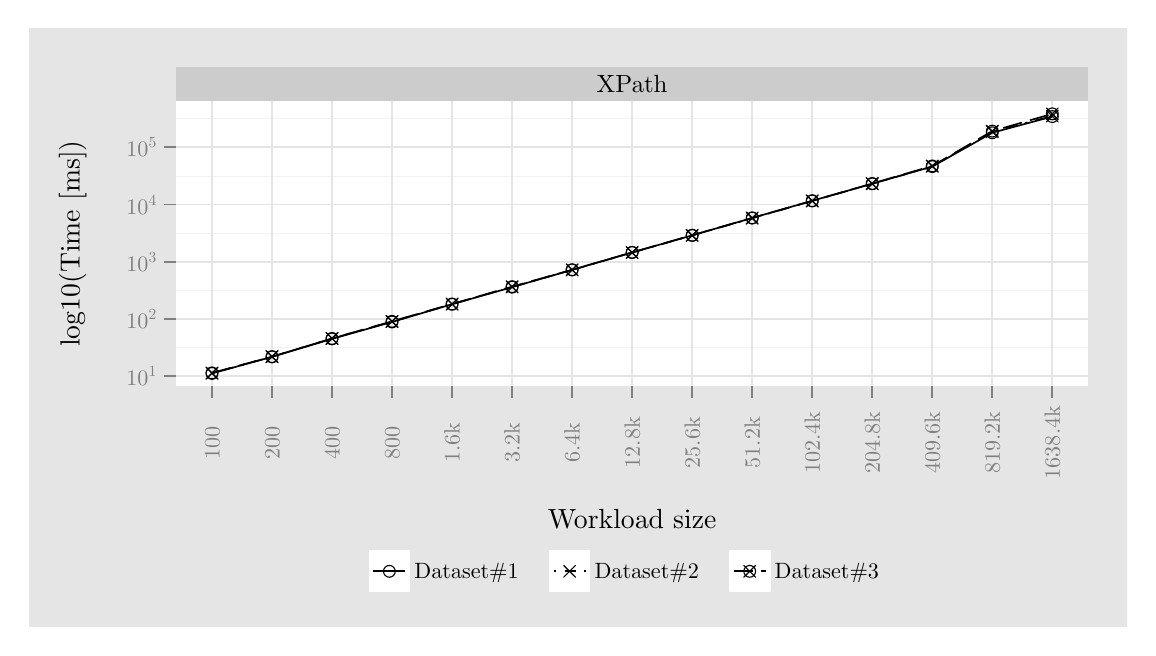
\begin{tikzpicture}[x=1pt,y=1pt]
\definecolor[named]{fillColor}{rgb}{1.00,1.00,1.00}
\path[use as bounding box,fill=fillColor,fill opacity=0.00] (0,0) rectangle (397.48,216.81);
\begin{scope}
\path[clip] (  0.00,  0.00) rectangle (397.48,216.81);
\definecolor[named]{drawColor}{rgb}{1.00,1.00,1.00}
\definecolor[named]{fillColor}{rgb}{0.90,0.90,0.90}

\path[draw=drawColor,line width= 0.6pt,line join=round,line cap=round,fill=fillColor] (  0.00,  0.00) rectangle (397.48,216.81);
\end{scope}
\begin{scope}
\path[clip] ( 53.58, 87.19) rectangle (383.26,190.36);
\definecolor[named]{fillColor}{rgb}{1.00,1.00,1.00}

\path[fill=fillColor] ( 53.58, 87.19) rectangle (383.26,190.36);
\definecolor[named]{drawColor}{rgb}{0.95,0.95,0.95}

\path[draw=drawColor,line width= 0.3pt,line join=round] ( 53.58,101.20) --
	(383.26,101.20);

\path[draw=drawColor,line width= 0.3pt,line join=round] ( 53.58,121.88) --
	(383.26,121.88);

\path[draw=drawColor,line width= 0.3pt,line join=round] ( 53.58,142.56) --
	(383.26,142.56);

\path[draw=drawColor,line width= 0.3pt,line join=round] ( 53.58,163.23) --
	(383.26,163.23);

\path[draw=drawColor,line width= 0.3pt,line join=round] ( 53.58,183.91) --
	(383.26,183.91);
\definecolor[named]{drawColor}{rgb}{0.90,0.90,0.90}

\path[draw=drawColor,line width= 0.6pt,line join=round] ( 53.58, 90.86) --
	(383.26, 90.86);

\path[draw=drawColor,line width= 0.6pt,line join=round] ( 53.58,111.54) --
	(383.26,111.54);

\path[draw=drawColor,line width= 0.6pt,line join=round] ( 53.58,132.22) --
	(383.26,132.22);

\path[draw=drawColor,line width= 0.6pt,line join=round] ( 53.58,152.89) --
	(383.26,152.89);

\path[draw=drawColor,line width= 0.6pt,line join=round] ( 53.58,173.57) --
	(383.26,173.57);

\path[draw=drawColor,line width= 0.6pt,line join=round] ( 66.60, 87.19) --
	( 66.60,190.36);

\path[draw=drawColor,line width= 0.6pt,line join=round] ( 88.29, 87.19) --
	( 88.29,190.36);

\path[draw=drawColor,line width= 0.6pt,line join=round] (109.97, 87.19) --
	(109.97,190.36);

\path[draw=drawColor,line width= 0.6pt,line join=round] (131.66, 87.19) --
	(131.66,190.36);

\path[draw=drawColor,line width= 0.6pt,line join=round] (153.35, 87.19) --
	(153.35,190.36);

\path[draw=drawColor,line width= 0.6pt,line join=round] (175.04, 87.19) --
	(175.04,190.36);

\path[draw=drawColor,line width= 0.6pt,line join=round] (196.73, 87.19) --
	(196.73,190.36);

\path[draw=drawColor,line width= 0.6pt,line join=round] (218.42, 87.19) --
	(218.42,190.36);

\path[draw=drawColor,line width= 0.6pt,line join=round] (240.11, 87.19) --
	(240.11,190.36);

\path[draw=drawColor,line width= 0.6pt,line join=round] (261.80, 87.19) --
	(261.80,190.36);

\path[draw=drawColor,line width= 0.6pt,line join=round] (283.49, 87.19) --
	(283.49,190.36);

\path[draw=drawColor,line width= 0.6pt,line join=round] (305.18, 87.19) --
	(305.18,190.36);

\path[draw=drawColor,line width= 0.6pt,line join=round] (326.87, 87.19) --
	(326.87,190.36);

\path[draw=drawColor,line width= 0.6pt,line join=round] (348.56, 87.19) --
	(348.56,190.36);

\path[draw=drawColor,line width= 0.6pt,line join=round] (370.25, 87.19) --
	(370.25,190.36);
\definecolor[named]{drawColor}{rgb}{0.00,0.00,0.00}

\path[draw=drawColor,line width= 0.6pt,line join=round] ( 66.60, 91.88) --
	( 88.29, 97.86) --
	(109.97,104.35) --
	(131.66,110.47) --
	(153.35,116.87) --
	(175.04,123.04) --
	(196.73,129.28) --
	(218.42,135.59) --
	(240.11,141.76) --
	(261.80,148.04) --
	(283.49,154.25) --
	(305.18,160.41) --
	(326.87,166.61) --
	(348.56,178.84) --
	(370.25,184.69);

\path[draw=drawColor,line width= 0.6pt,dash pattern=on 1pt off 3pt on 4pt off 3pt ,line join=round] ( 66.60, 91.91) --
	( 88.29, 97.90) --
	(109.97,104.49) --
	(131.66,110.58) --
	(153.35,116.90) --
	(175.04,123.11) --
	(196.73,129.26) --
	(218.42,135.53) --
	(240.11,141.73) --
	(261.80,147.96) --
	(283.49,154.19) --
	(305.18,160.40) --
	(326.87,166.66) --
	(348.56,179.29) --
	(370.25,184.85);

\path[draw=drawColor,line width= 0.6pt,dash pattern=on 7pt off 3pt ,line join=round] ( 66.60, 92.07) --
	( 88.29, 97.92) --
	(109.97,104.50) --
	(131.66,110.69) --
	(153.35,116.95) --
	(175.04,123.22) --
	(196.73,129.32) --
	(218.42,135.59) --
	(240.11,141.79) --
	(261.80,148.05) --
	(283.49,154.22) --
	(305.18,160.48) --
	(326.87,166.85) --
	(348.56,179.43) --
	(370.25,185.67);

\path[draw=drawColor,line width= 0.4pt,line join=round,line cap=round] ( 66.60, 91.88) circle (  2.13);

\path[draw=drawColor,line width= 0.4pt,line join=round,line cap=round] ( 88.29, 97.86) circle (  2.13);

\path[draw=drawColor,line width= 0.4pt,line join=round,line cap=round] (109.97,104.35) circle (  2.13);

\path[draw=drawColor,line width= 0.4pt,line join=round,line cap=round] (131.66,110.47) circle (  2.13);

\path[draw=drawColor,line width= 0.4pt,line join=round,line cap=round] (153.35,116.87) circle (  2.13);

\path[draw=drawColor,line width= 0.4pt,line join=round,line cap=round] (175.04,123.04) circle (  2.13);

\path[draw=drawColor,line width= 0.4pt,line join=round,line cap=round] (196.73,129.28) circle (  2.13);

\path[draw=drawColor,line width= 0.4pt,line join=round,line cap=round] (218.42,135.59) circle (  2.13);

\path[draw=drawColor,line width= 0.4pt,line join=round,line cap=round] (240.11,141.76) circle (  2.13);

\path[draw=drawColor,line width= 0.4pt,line join=round,line cap=round] (261.80,148.04) circle (  2.13);

\path[draw=drawColor,line width= 0.4pt,line join=round,line cap=round] (283.49,154.25) circle (  2.13);

\path[draw=drawColor,line width= 0.4pt,line join=round,line cap=round] (305.18,160.41) circle (  2.13);

\path[draw=drawColor,line width= 0.4pt,line join=round,line cap=round] (326.87,166.61) circle (  2.13);

\path[draw=drawColor,line width= 0.4pt,line join=round,line cap=round] (348.56,178.84) circle (  2.13);

\path[draw=drawColor,line width= 0.4pt,line join=round,line cap=round] (370.25,184.69) circle (  2.13);

\path[draw=drawColor,line width= 0.4pt,line join=round,line cap=round] ( 64.46, 89.77) -- ( 68.73, 94.04);

\path[draw=drawColor,line width= 0.4pt,line join=round,line cap=round] ( 64.46, 94.04) -- ( 68.73, 89.77);

\path[draw=drawColor,line width= 0.4pt,line join=round,line cap=round] ( 86.15, 95.77) -- ( 90.42,100.04);

\path[draw=drawColor,line width= 0.4pt,line join=round,line cap=round] ( 86.15,100.04) -- ( 90.42, 95.77);

\path[draw=drawColor,line width= 0.4pt,line join=round,line cap=round] (107.84,102.36) -- (112.11,106.63);

\path[draw=drawColor,line width= 0.4pt,line join=round,line cap=round] (107.84,106.63) -- (112.11,102.36);

\path[draw=drawColor,line width= 0.4pt,line join=round,line cap=round] (129.53,108.45) -- (133.80,112.72);

\path[draw=drawColor,line width= 0.4pt,line join=round,line cap=round] (129.53,112.72) -- (133.80,108.45);

\path[draw=drawColor,line width= 0.4pt,line join=round,line cap=round] (151.22,114.77) -- (155.49,119.04);

\path[draw=drawColor,line width= 0.4pt,line join=round,line cap=round] (151.22,119.04) -- (155.49,114.77);

\path[draw=drawColor,line width= 0.4pt,line join=round,line cap=round] (172.91,120.98) -- (177.18,125.24);

\path[draw=drawColor,line width= 0.4pt,line join=round,line cap=round] (172.91,125.24) -- (177.18,120.98);

\path[draw=drawColor,line width= 0.4pt,line join=round,line cap=round] (194.60,127.12) -- (198.87,131.39);

\path[draw=drawColor,line width= 0.4pt,line join=round,line cap=round] (194.60,131.39) -- (198.87,127.12);

\path[draw=drawColor,line width= 0.4pt,line join=round,line cap=round] (216.29,133.39) -- (220.55,137.66);

\path[draw=drawColor,line width= 0.4pt,line join=round,line cap=round] (216.29,137.66) -- (220.55,133.39);

\path[draw=drawColor,line width= 0.4pt,line join=round,line cap=round] (237.98,139.60) -- (242.24,143.87);

\path[draw=drawColor,line width= 0.4pt,line join=round,line cap=round] (237.98,143.87) -- (242.24,139.60);

\path[draw=drawColor,line width= 0.4pt,line join=round,line cap=round] (259.67,145.82) -- (263.93,150.09);

\path[draw=drawColor,line width= 0.4pt,line join=round,line cap=round] (259.67,150.09) -- (263.93,145.82);

\path[draw=drawColor,line width= 0.4pt,line join=round,line cap=round] (281.35,152.05) -- (285.62,156.32);

\path[draw=drawColor,line width= 0.4pt,line join=round,line cap=round] (281.35,156.32) -- (285.62,152.05);

\path[draw=drawColor,line width= 0.4pt,line join=round,line cap=round] (303.04,158.27) -- (307.31,162.54);

\path[draw=drawColor,line width= 0.4pt,line join=round,line cap=round] (303.04,162.54) -- (307.31,158.27);

\path[draw=drawColor,line width= 0.4pt,line join=round,line cap=round] (324.73,164.53) -- (329.00,168.79);

\path[draw=drawColor,line width= 0.4pt,line join=round,line cap=round] (324.73,168.79) -- (329.00,164.53);

\path[draw=drawColor,line width= 0.4pt,line join=round,line cap=round] (346.42,177.15) -- (350.69,181.42);

\path[draw=drawColor,line width= 0.4pt,line join=round,line cap=round] (346.42,181.42) -- (350.69,177.15);

\path[draw=drawColor,line width= 0.4pt,line join=round,line cap=round] (368.11,182.72) -- (372.38,186.98);

\path[draw=drawColor,line width= 0.4pt,line join=round,line cap=round] (368.11,186.98) -- (372.38,182.72);

\path[draw=drawColor,line width= 0.4pt,line join=round,line cap=round] ( 66.60, 92.07) circle (  2.13);

\path[draw=drawColor,line width= 0.4pt,line join=round,line cap=round] ( 64.46, 89.93) -- ( 68.73, 94.20);

\path[draw=drawColor,line width= 0.4pt,line join=round,line cap=round] ( 64.46, 94.20) -- ( 68.73, 89.93);

\path[draw=drawColor,line width= 0.4pt,line join=round,line cap=round] ( 88.29, 97.92) circle (  2.13);

\path[draw=drawColor,line width= 0.4pt,line join=round,line cap=round] ( 86.15, 95.79) -- ( 90.42,100.05);

\path[draw=drawColor,line width= 0.4pt,line join=round,line cap=round] ( 86.15,100.05) -- ( 90.42, 95.79);

\path[draw=drawColor,line width= 0.4pt,line join=round,line cap=round] (109.97,104.50) circle (  2.13);

\path[draw=drawColor,line width= 0.4pt,line join=round,line cap=round] (107.84,102.36) -- (112.11,106.63);

\path[draw=drawColor,line width= 0.4pt,line join=round,line cap=round] (107.84,106.63) -- (112.11,102.36);

\path[draw=drawColor,line width= 0.4pt,line join=round,line cap=round] (131.66,110.69) circle (  2.13);

\path[draw=drawColor,line width= 0.4pt,line join=round,line cap=round] (129.53,108.56) -- (133.80,112.83);

\path[draw=drawColor,line width= 0.4pt,line join=round,line cap=round] (129.53,112.83) -- (133.80,108.56);

\path[draw=drawColor,line width= 0.4pt,line join=round,line cap=round] (153.35,116.95) circle (  2.13);

\path[draw=drawColor,line width= 0.4pt,line join=round,line cap=round] (151.22,114.82) -- (155.49,119.09);

\path[draw=drawColor,line width= 0.4pt,line join=round,line cap=round] (151.22,119.09) -- (155.49,114.82);

\path[draw=drawColor,line width= 0.4pt,line join=round,line cap=round] (175.04,123.22) circle (  2.13);

\path[draw=drawColor,line width= 0.4pt,line join=round,line cap=round] (172.91,121.09) -- (177.18,125.35);

\path[draw=drawColor,line width= 0.4pt,line join=round,line cap=round] (172.91,125.35) -- (177.18,121.09);

\path[draw=drawColor,line width= 0.4pt,line join=round,line cap=round] (196.73,129.32) circle (  2.13);

\path[draw=drawColor,line width= 0.4pt,line join=round,line cap=round] (194.60,127.18) -- (198.87,131.45);

\path[draw=drawColor,line width= 0.4pt,line join=round,line cap=round] (194.60,131.45) -- (198.87,127.18);

\path[draw=drawColor,line width= 0.4pt,line join=round,line cap=round] (218.42,135.59) circle (  2.13);

\path[draw=drawColor,line width= 0.4pt,line join=round,line cap=round] (216.29,133.46) -- (220.55,137.72);

\path[draw=drawColor,line width= 0.4pt,line join=round,line cap=round] (216.29,137.72) -- (220.55,133.46);

\path[draw=drawColor,line width= 0.4pt,line join=round,line cap=round] (240.11,141.79) circle (  2.13);

\path[draw=drawColor,line width= 0.4pt,line join=round,line cap=round] (237.98,139.66) -- (242.24,143.92);

\path[draw=drawColor,line width= 0.4pt,line join=round,line cap=round] (237.98,143.92) -- (242.24,139.66);

\path[draw=drawColor,line width= 0.4pt,line join=round,line cap=round] (261.80,148.05) circle (  2.13);

\path[draw=drawColor,line width= 0.4pt,line join=round,line cap=round] (259.67,145.92) -- (263.93,150.19);

\path[draw=drawColor,line width= 0.4pt,line join=round,line cap=round] (259.67,150.19) -- (263.93,145.92);

\path[draw=drawColor,line width= 0.4pt,line join=round,line cap=round] (283.49,154.22) circle (  2.13);

\path[draw=drawColor,line width= 0.4pt,line join=round,line cap=round] (281.35,152.08) -- (285.62,156.35);

\path[draw=drawColor,line width= 0.4pt,line join=round,line cap=round] (281.35,156.35) -- (285.62,152.08);

\path[draw=drawColor,line width= 0.4pt,line join=round,line cap=round] (305.18,160.48) circle (  2.13);

\path[draw=drawColor,line width= 0.4pt,line join=round,line cap=round] (303.04,158.35) -- (307.31,162.62);

\path[draw=drawColor,line width= 0.4pt,line join=round,line cap=round] (303.04,162.62) -- (307.31,158.35);

\path[draw=drawColor,line width= 0.4pt,line join=round,line cap=round] (326.87,166.85) circle (  2.13);

\path[draw=drawColor,line width= 0.4pt,line join=round,line cap=round] (324.73,164.72) -- (329.00,168.99);

\path[draw=drawColor,line width= 0.4pt,line join=round,line cap=round] (324.73,168.99) -- (329.00,164.72);

\path[draw=drawColor,line width= 0.4pt,line join=round,line cap=round] (348.56,179.43) circle (  2.13);

\path[draw=drawColor,line width= 0.4pt,line join=round,line cap=round] (346.42,177.30) -- (350.69,181.57);

\path[draw=drawColor,line width= 0.4pt,line join=round,line cap=round] (346.42,181.57) -- (350.69,177.30);

\path[draw=drawColor,line width= 0.4pt,line join=round,line cap=round] (370.25,185.67) circle (  2.13);

\path[draw=drawColor,line width= 0.4pt,line join=round,line cap=round] (368.11,183.54) -- (372.38,187.81);

\path[draw=drawColor,line width= 0.4pt,line join=round,line cap=round] (368.11,187.81) -- (372.38,183.54);
\end{scope}
\begin{scope}
\path[clip] (  0.00,  0.00) rectangle (397.48,216.81);
\definecolor[named]{fillColor}{rgb}{0.80,0.80,0.80}

\path[fill=fillColor] ( 53.58,190.36) rectangle (383.26,202.58);
\definecolor[named]{drawColor}{rgb}{0.00,0.00,0.00}

\node[text=drawColor,anchor=base,inner sep=0pt, outer sep=0pt, scale=  0.90] at (218.42,193.37) {XPath};
\end{scope}
\begin{scope}
\path[clip] (  0.00,  0.00) rectangle (397.48,216.81);
\definecolor[named]{drawColor}{rgb}{0.50,0.50,0.50}

\node[text=drawColor,anchor=base west,inner sep=0pt, outer sep=0pt, scale=  0.80] at ( 35.67, 87.43) {10};

\node[text=drawColor,anchor=base west,inner sep=0pt, outer sep=0pt, scale=  0.56] at ( 43.67, 90.70) {1};

\node[text=drawColor,anchor=base west,inner sep=0pt, outer sep=0pt, scale=  0.80] at ( 35.67,108.11) {10};

\node[text=drawColor,anchor=base west,inner sep=0pt, outer sep=0pt, scale=  0.56] at ( 43.67,111.38) {2};

\node[text=drawColor,anchor=base west,inner sep=0pt, outer sep=0pt, scale=  0.80] at ( 35.67,128.79) {10};

\node[text=drawColor,anchor=base west,inner sep=0pt, outer sep=0pt, scale=  0.56] at ( 43.67,132.06) {3};

\node[text=drawColor,anchor=base west,inner sep=0pt, outer sep=0pt, scale=  0.80] at ( 35.67,149.46) {10};

\node[text=drawColor,anchor=base west,inner sep=0pt, outer sep=0pt, scale=  0.56] at ( 43.67,152.73) {4};

\node[text=drawColor,anchor=base west,inner sep=0pt, outer sep=0pt, scale=  0.80] at ( 35.67,170.14) {10};

\node[text=drawColor,anchor=base west,inner sep=0pt, outer sep=0pt, scale=  0.56] at ( 43.67,173.41) {5};
\end{scope}
\begin{scope}
\path[clip] (  0.00,  0.00) rectangle (397.48,216.81);
\definecolor[named]{drawColor}{rgb}{0.50,0.50,0.50}

\path[draw=drawColor,line width= 0.6pt,line join=round] ( 49.31, 90.86) --
	( 53.58, 90.86);

\path[draw=drawColor,line width= 0.6pt,line join=round] ( 49.31,111.54) --
	( 53.58,111.54);

\path[draw=drawColor,line width= 0.6pt,line join=round] ( 49.31,132.22) --
	( 53.58,132.22);

\path[draw=drawColor,line width= 0.6pt,line join=round] ( 49.31,152.89) --
	( 53.58,152.89);

\path[draw=drawColor,line width= 0.6pt,line join=round] ( 49.31,173.57) --
	( 53.58,173.57);
\end{scope}
\begin{scope}
\path[clip] (  0.00,  0.00) rectangle (397.48,216.81);
\definecolor[named]{drawColor}{rgb}{0.50,0.50,0.50}

\path[draw=drawColor,line width= 0.6pt,line join=round] ( 66.60, 82.92) --
	( 66.60, 87.19);

\path[draw=drawColor,line width= 0.6pt,line join=round] ( 88.29, 82.92) --
	( 88.29, 87.19);

\path[draw=drawColor,line width= 0.6pt,line join=round] (109.97, 82.92) --
	(109.97, 87.19);

\path[draw=drawColor,line width= 0.6pt,line join=round] (131.66, 82.92) --
	(131.66, 87.19);

\path[draw=drawColor,line width= 0.6pt,line join=round] (153.35, 82.92) --
	(153.35, 87.19);

\path[draw=drawColor,line width= 0.6pt,line join=round] (175.04, 82.92) --
	(175.04, 87.19);

\path[draw=drawColor,line width= 0.6pt,line join=round] (196.73, 82.92) --
	(196.73, 87.19);

\path[draw=drawColor,line width= 0.6pt,line join=round] (218.42, 82.92) --
	(218.42, 87.19);

\path[draw=drawColor,line width= 0.6pt,line join=round] (240.11, 82.92) --
	(240.11, 87.19);

\path[draw=drawColor,line width= 0.6pt,line join=round] (261.80, 82.92) --
	(261.80, 87.19);

\path[draw=drawColor,line width= 0.6pt,line join=round] (283.49, 82.92) --
	(283.49, 87.19);

\path[draw=drawColor,line width= 0.6pt,line join=round] (305.18, 82.92) --
	(305.18, 87.19);

\path[draw=drawColor,line width= 0.6pt,line join=round] (326.87, 82.92) --
	(326.87, 87.19);

\path[draw=drawColor,line width= 0.6pt,line join=round] (348.56, 82.92) --
	(348.56, 87.19);

\path[draw=drawColor,line width= 0.6pt,line join=round] (370.25, 82.92) --
	(370.25, 87.19);
\end{scope}
\begin{scope}
\path[clip] (  0.00,  0.00) rectangle (397.48,216.81);
\definecolor[named]{drawColor}{rgb}{0.50,0.50,0.50}

\node[text=drawColor,rotate= 90.00,anchor=base,inner sep=0pt, outer sep=0pt, scale=  0.80] at ( 69.35, 66.85) {100};

\node[text=drawColor,rotate= 90.00,anchor=base,inner sep=0pt, outer sep=0pt, scale=  0.80] at ( 91.04, 66.85) {200};

\node[text=drawColor,rotate= 90.00,anchor=base,inner sep=0pt, outer sep=0pt, scale=  0.80] at (112.73, 66.85) {400};

\node[text=drawColor,rotate= 90.00,anchor=base,inner sep=0pt, outer sep=0pt, scale=  0.80] at (134.42, 66.85) {800};

\node[text=drawColor,rotate= 90.00,anchor=base,inner sep=0pt, outer sep=0pt, scale=  0.80] at (156.11, 66.85) {1.6k};

\node[text=drawColor,rotate= 90.00,anchor=base,inner sep=0pt, outer sep=0pt, scale=  0.80] at (177.80, 66.85) {3.2k};

\node[text=drawColor,rotate= 90.00,anchor=base,inner sep=0pt, outer sep=0pt, scale=  0.80] at (199.49, 66.85) {6.4k};

\node[text=drawColor,rotate= 90.00,anchor=base,inner sep=0pt, outer sep=0pt, scale=  0.80] at (221.18, 66.85) {12.8k};

\node[text=drawColor,rotate= 90.00,anchor=base,inner sep=0pt, outer sep=0pt, scale=  0.80] at (242.86, 66.85) {25.6k};

\node[text=drawColor,rotate= 90.00,anchor=base,inner sep=0pt, outer sep=0pt, scale=  0.80] at (264.55, 66.85) {51.2k};

\node[text=drawColor,rotate= 90.00,anchor=base,inner sep=0pt, outer sep=0pt, scale=  0.80] at (286.24, 66.85) {102.4k};

\node[text=drawColor,rotate= 90.00,anchor=base,inner sep=0pt, outer sep=0pt, scale=  0.80] at (307.93, 66.85) {204.8k};

\node[text=drawColor,rotate= 90.00,anchor=base,inner sep=0pt, outer sep=0pt, scale=  0.80] at (329.62, 66.85) {409.6k};

\node[text=drawColor,rotate= 90.00,anchor=base,inner sep=0pt, outer sep=0pt, scale=  0.80] at (351.31, 66.85) {819.2k};

\node[text=drawColor,rotate= 90.00,anchor=base,inner sep=0pt, outer sep=0pt, scale=  0.80] at (373.00, 66.85) {1638.4k};
\end{scope}
\begin{scope}
\path[clip] (  0.00,  0.00) rectangle (397.48,216.81);
\definecolor[named]{drawColor}{rgb}{0.00,0.00,0.00}

\node[text=drawColor,anchor=base,inner sep=0pt, outer sep=0pt, scale=  1.00] at (218.42, 35.91) {Workload size};
\end{scope}
\begin{scope}
\path[clip] (  0.00,  0.00) rectangle (397.48,216.81);
\definecolor[named]{drawColor}{rgb}{0.00,0.00,0.00}

\node[text=drawColor,rotate= 90.00,anchor=base,inner sep=0pt, outer sep=0pt, scale=  1.00] at ( 18.80,138.77) {log10(Time [ms])};
\end{scope}
\begin{scope}
\path[clip] (  0.00,  0.00) rectangle (397.48,216.81);
\definecolor[named]{fillColor}{rgb}{0.90,0.90,0.90}

\path[fill=fillColor] (115.60,  8.87) rectangle (321.24, 31.86);
\end{scope}
\begin{scope}
\path[clip] (  0.00,  0.00) rectangle (397.48,216.81);
\definecolor[named]{drawColor}{rgb}{1.00,1.00,1.00}
\definecolor[named]{fillColor}{rgb}{1.00,1.00,1.00}

\path[draw=drawColor,line width= 0.6pt,line join=round,line cap=round,fill=fillColor] (123.48, 13.14) rectangle (137.93, 27.59);
\end{scope}
\begin{scope}
\path[clip] (  0.00,  0.00) rectangle (397.48,216.81);
\definecolor[named]{drawColor}{rgb}{0.00,0.00,0.00}

\path[draw=drawColor,line width= 0.6pt,line join=round] (124.92, 20.36) -- (136.49, 20.36);
\end{scope}
\begin{scope}
\path[clip] (  0.00,  0.00) rectangle (397.48,216.81);
\definecolor[named]{drawColor}{rgb}{0.00,0.00,0.00}

\path[draw=drawColor,line width= 0.4pt,line join=round,line cap=round] (130.70, 20.36) circle (  2.13);
\end{scope}
\begin{scope}
\path[clip] (  0.00,  0.00) rectangle (397.48,216.81);
\definecolor[named]{drawColor}{rgb}{1.00,1.00,1.00}
\definecolor[named]{fillColor}{rgb}{1.00,1.00,1.00}

\path[draw=drawColor,line width= 0.6pt,line join=round,line cap=round,fill=fillColor] (188.58, 13.14) rectangle (203.03, 27.59);
\end{scope}
\begin{scope}
\path[clip] (  0.00,  0.00) rectangle (397.48,216.81);
\definecolor[named]{drawColor}{rgb}{0.00,0.00,0.00}

\path[draw=drawColor,line width= 0.6pt,dash pattern=on 1pt off 3pt on 4pt off 3pt ,line join=round] (190.03, 20.36) -- (201.59, 20.36);
\end{scope}
\begin{scope}
\path[clip] (  0.00,  0.00) rectangle (397.48,216.81);
\definecolor[named]{drawColor}{rgb}{0.00,0.00,0.00}

\path[draw=drawColor,line width= 0.4pt,line join=round,line cap=round] (193.67, 18.23) -- (197.94, 22.50);

\path[draw=drawColor,line width= 0.4pt,line join=round,line cap=round] (193.67, 22.50) -- (197.94, 18.23);
\end{scope}
\begin{scope}
\path[clip] (  0.00,  0.00) rectangle (397.48,216.81);
\definecolor[named]{drawColor}{rgb}{1.00,1.00,1.00}
\definecolor[named]{fillColor}{rgb}{1.00,1.00,1.00}

\path[draw=drawColor,line width= 0.6pt,line join=round,line cap=round,fill=fillColor] (253.68, 13.14) rectangle (268.14, 27.59);
\end{scope}
\begin{scope}
\path[clip] (  0.00,  0.00) rectangle (397.48,216.81);
\definecolor[named]{drawColor}{rgb}{0.00,0.00,0.00}

\path[draw=drawColor,line width= 0.6pt,dash pattern=on 7pt off 3pt ,line join=round] (255.13, 20.36) -- (266.69, 20.36);
\end{scope}
\begin{scope}
\path[clip] (  0.00,  0.00) rectangle (397.48,216.81);
\definecolor[named]{drawColor}{rgb}{0.00,0.00,0.00}

\path[draw=drawColor,line width= 0.4pt,line join=round,line cap=round] (260.91, 20.36) circle (  2.13);

\path[draw=drawColor,line width= 0.4pt,line join=round,line cap=round] (258.77, 18.23) -- (263.04, 22.50);

\path[draw=drawColor,line width= 0.4pt,line join=round,line cap=round] (258.77, 22.50) -- (263.04, 18.23);
\end{scope}
\begin{scope}
\path[clip] (  0.00,  0.00) rectangle (397.48,216.81);
\definecolor[named]{drawColor}{rgb}{0.00,0.00,0.00}

\node[text=drawColor,anchor=base west,inner sep=0pt, outer sep=0pt, scale=  0.80] at (139.74, 17.61) {Dataset\#1 $\;\;\;$};
\end{scope}
\begin{scope}
\path[clip] (  0.00,  0.00) rectangle (397.48,216.81);
\definecolor[named]{drawColor}{rgb}{0.00,0.00,0.00}

\node[text=drawColor,anchor=base west,inner sep=0pt, outer sep=0pt, scale=  0.80] at (204.84, 17.61) {Dataset\#2 $\;\;\;$};
\end{scope}
\begin{scope}
\path[clip] (  0.00,  0.00) rectangle (397.48,216.81);
\definecolor[named]{drawColor}{rgb}{0.00,0.00,0.00}

\node[text=drawColor,anchor=base west,inner sep=0pt, outer sep=0pt, scale=  0.80] at (269.94, 17.61) {Dataset\#3 $\;\;\;$};
\end{scope}
\end{tikzpicture}

 }
 \caption[Impact of structure on XPath\index{XPath} query phase]{Impact of structure on XPath\index{XPath} query phase.}
 \label{fig:experimentation:performance:search:processing-phases-xpath-levels}
\end{figure}
\end{comment}

\subparagraph{Discussion}

There is a significant linear increase in the search\index{Search} query response times before the workload\index{Workload} size goes beyond \num{409600}, with the Parsing\index{Parsing} and XPath\index{XPath} times remaining constant as the traversal times change.

%%\paragraph{Conclusion}
%%xxx

\subsubsection{Indexing operations}
\label{sec:evaluation:performance:indexing}

The integration of \glspl{dls} with indexing\index{Index} services is
increasingly becoming common to facilitate seamless discovery of information
through search\index{Search} and browse\index{Browse} services. The experiments conducted for the index
evaluation aspect were aimed at benchmarking various indexing\index{Index} operations
associated with digital collections.

The Apache Solr\index{Apache!Solr} search\index{Search} platform was deployed within a Jetty\index{Jetty} Servlet engine, and
subsequently integrated with the 15 workloads.\index{Workload} The workloads were conveniently
set-up as 15 separate Apache Solr Cores\index{Apache!Solr!Cores} and the following factors were
investigated relative to the different workload\index{Workload} sizes described in Section~\ref{sec:evaluation:performance:test-environment:workload-design}.

\begin{itemize}
 \item Batch indexing\index{Index} of collections
 \item Incremental updates to existing collections
\end{itemize}

% 
% Not necessary to include this figure in manuscript
\begin{comment}
\begin{figure}
 \centering
 \framebox[\textwidth]{%
\input{chapter07/figures/experimentation.performance.indexing.solr-core-set-up.tex}
 }
 \caption[Apache Solr Core set-up]{Experiment set-up for Apache Solr Cores within Jetty Servlet engine}
 \label{fig:experimentation:performance:indexing:solr-core-set-up}
\end{figure}
\end{comment}

\paragraph{Experiment: Batch collection indexing\index{Index} benchmarks}
\label{sec:evaluation:performance:indexing:experiment1}

Batch indexing\index{Index} of collections is a common use-case; for instance, storage and
retrieval systems will in certain instances require re-indexing of content when
records have been updated with new values. This experiment was aimed at
benchmarking the batch indexing\index{Index} of varying workloads.\index{Workload}

\subparagraph{Methodology}

The Apache Solr Data Import Request Handler\index{Apache!Solr!Data Import Handler} \citep{SolrDIH2012} was
configured for all the 15 workload\index{Workload} cores to perform full builds. A full
data-import command was then issued, and repeated 5 times, for each of the 15
workload cores. The minimum time taken to perform successful data-import
operations was then recorded.

\subparagraph{Results}

The batch indexing\index{Index} experiment results are shown in Table~\ref{tab:experimentation:performance:indexing:batch-indexing} and Figure~\ref{fig:experimentation:performance:indexing:index-throughput}.

\subparagraph{Discussion}

The results strongly indicate that there is a linear relationship between the workload\index{Workload} size and the resulting index\index{Index} size, with an average ratio of 1:2. This is largely as a result of indexing\index{Index} all the \num{15} Dublin Core\index{Dublin Core} repeatable fields. In addition, all the record fields were stored in the index\index{Index} when conducting the experiment. In an ideal scenario, only relevant fields would have to be indexed and stored, significantly reducing the resulting index\index{Index} size.

The indexing\index{Index} operation throughput generally increases with increasing workload, reaching a peak value of \num{803} documents/second at workload\index{Workload} $W9$---as shown in Figure~\ref{fig:experimentation:performance:indexing:index-throughput}, after which it plummets. This scenario is attributed to the fact that Apache Solr indexing\index{Index} is, in part, dependent on the size on the index---the index\index{Index} size linearly increases with workload\index{Workload} size. Furthermore, the 2 GB RAM on the graduate becomes inadequate as the workload\index{Workload} increases, thus degrading the performance.

% 
% Plot merged within facet showing size, times& throughout
\begin{comment}
\begin{figure}
 \centering
 \framebox[\textwidth]{%
% Created by tikzDevice version 0.6.2-92-0ad2792 on 2013-03-28 13:04:04
% !TEX encoding = UTF-8 Unicode
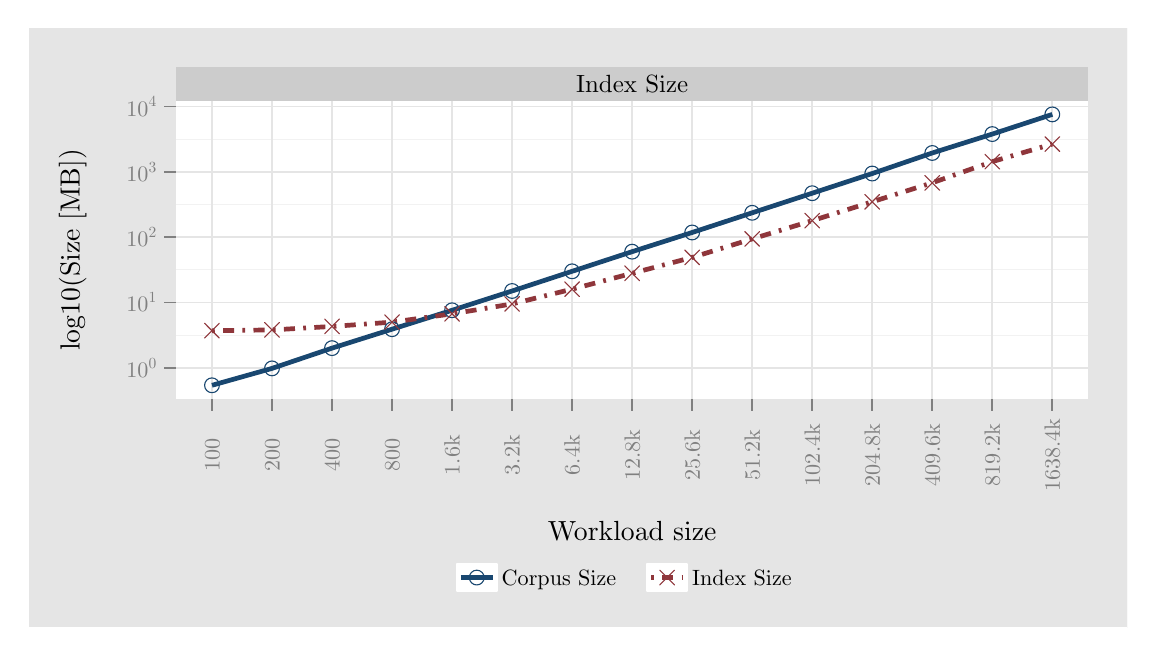
\begin{tikzpicture}[x=1pt,y=1pt]
\definecolor[named]{fillColor}{rgb}{1.00,1.00,1.00}
\path[use as bounding box,fill=fillColor,fill opacity=0.00] (0,0) rectangle (397.48,216.81);
\begin{scope}
\path[clip] (  0.00,  0.00) rectangle (397.48,216.81);
\definecolor[named]{drawColor}{rgb}{1.00,1.00,1.00}
\definecolor[named]{fillColor}{rgb}{0.90,0.90,0.90}

\path[draw=drawColor,line width= 0.6pt,line join=round,line cap=round,fill=fillColor] (  0.00,  0.00) rectangle (397.48,216.81);
\end{scope}
\begin{scope}
\path[clip] ( 53.58, 82.69) rectangle (383.26,190.36);
\definecolor[named]{fillColor}{rgb}{1.00,1.00,1.00}

\path[fill=fillColor] ( 53.58, 82.69) rectangle (383.26,190.36);
\definecolor[named]{drawColor}{rgb}{0.95,0.95,0.95}

\path[draw=drawColor,line width= 0.3pt,line join=round] ( 53.58,105.70) --
	(383.26,105.70);

\path[draw=drawColor,line width= 0.3pt,line join=round] ( 53.58,129.31) --
	(383.26,129.31);

\path[draw=drawColor,line width= 0.3pt,line join=round] ( 53.58,152.91) --
	(383.26,152.91);

\path[draw=drawColor,line width= 0.3pt,line join=round] ( 53.58,176.51) --
	(383.26,176.51);
\definecolor[named]{drawColor}{rgb}{0.90,0.90,0.90}

\path[draw=drawColor,line width= 0.6pt,line join=round] ( 53.58, 93.90) --
	(383.26, 93.90);

\path[draw=drawColor,line width= 0.6pt,line join=round] ( 53.58,117.50) --
	(383.26,117.50);

\path[draw=drawColor,line width= 0.6pt,line join=round] ( 53.58,141.11) --
	(383.26,141.11);

\path[draw=drawColor,line width= 0.6pt,line join=round] ( 53.58,164.71) --
	(383.26,164.71);

\path[draw=drawColor,line width= 0.6pt,line join=round] ( 53.58,188.31) --
	(383.26,188.31);

\path[draw=drawColor,line width= 0.6pt,line join=round] ( 66.60, 82.69) --
	( 66.60,190.36);

\path[draw=drawColor,line width= 0.6pt,line join=round] ( 88.29, 82.69) --
	( 88.29,190.36);

\path[draw=drawColor,line width= 0.6pt,line join=round] (109.97, 82.69) --
	(109.97,190.36);

\path[draw=drawColor,line width= 0.6pt,line join=round] (131.66, 82.69) --
	(131.66,190.36);

\path[draw=drawColor,line width= 0.6pt,line join=round] (153.35, 82.69) --
	(153.35,190.36);

\path[draw=drawColor,line width= 0.6pt,line join=round] (175.04, 82.69) --
	(175.04,190.36);

\path[draw=drawColor,line width= 0.6pt,line join=round] (196.73, 82.69) --
	(196.73,190.36);

\path[draw=drawColor,line width= 0.6pt,line join=round] (218.42, 82.69) --
	(218.42,190.36);

\path[draw=drawColor,line width= 0.6pt,line join=round] (240.11, 82.69) --
	(240.11,190.36);

\path[draw=drawColor,line width= 0.6pt,line join=round] (261.80, 82.69) --
	(261.80,190.36);

\path[draw=drawColor,line width= 0.6pt,line join=round] (283.49, 82.69) --
	(283.49,190.36);

\path[draw=drawColor,line width= 0.6pt,line join=round] (305.18, 82.69) --
	(305.18,190.36);

\path[draw=drawColor,line width= 0.6pt,line join=round] (326.87, 82.69) --
	(326.87,190.36);

\path[draw=drawColor,line width= 0.6pt,line join=round] (348.56, 82.69) --
	(348.56,190.36);

\path[draw=drawColor,line width= 0.6pt,line join=round] (370.25, 82.69) --
	(370.25,190.36);
\definecolor[named]{drawColor}{rgb}{0.10,0.28,0.44}

\path[draw=drawColor,line width= 1.7pt,line join=round] ( 66.60, 87.58) --
	( 88.29, 93.69) --
	(109.97,101.01) --
	(131.66,107.85) --
	(153.35,114.69) --
	(175.04,121.66) --
	(196.73,128.77) --
	(218.42,135.87) --
	(240.11,142.80) --
	(261.80,149.91) --
	(283.49,156.99) --
	(305.18,164.10) --
	(326.87,171.53) --
	(348.56,178.36) --
	(370.25,185.47);
\definecolor[named]{drawColor}{rgb}{0.56,0.21,0.23}

\path[draw=drawColor,line width= 1.7pt,dash pattern=on 1pt off 3pt on 4pt off 3pt ,line join=round] ( 66.60,107.31) --
	( 88.29,107.59) --
	(109.97,108.85) --
	(131.66,110.40) --
	(153.35,113.40) --
	(175.04,116.98) --
	(196.73,122.32) --
	(218.42,128.06) --
	(240.11,133.79) --
	(261.80,140.47) --
	(283.49,147.07) --
	(305.18,153.89) --
	(326.87,160.76) --
	(348.56,168.40) --
	(370.25,174.75);
\definecolor[named]{drawColor}{rgb}{0.10,0.28,0.44}

\path[draw=drawColor,line width= 0.4pt,line join=round,line cap=round] ( 66.60, 87.58) circle (  2.67);

\path[draw=drawColor,line width= 0.4pt,line join=round,line cap=round] ( 88.29, 93.69) circle (  2.67);

\path[draw=drawColor,line width= 0.4pt,line join=round,line cap=round] (109.97,101.01) circle (  2.67);

\path[draw=drawColor,line width= 0.4pt,line join=round,line cap=round] (131.66,107.85) circle (  2.67);

\path[draw=drawColor,line width= 0.4pt,line join=round,line cap=round] (153.35,114.69) circle (  2.67);

\path[draw=drawColor,line width= 0.4pt,line join=round,line cap=round] (175.04,121.66) circle (  2.67);

\path[draw=drawColor,line width= 0.4pt,line join=round,line cap=round] (196.73,128.77) circle (  2.67);

\path[draw=drawColor,line width= 0.4pt,line join=round,line cap=round] (218.42,135.87) circle (  2.67);

\path[draw=drawColor,line width= 0.4pt,line join=round,line cap=round] (240.11,142.80) circle (  2.67);

\path[draw=drawColor,line width= 0.4pt,line join=round,line cap=round] (261.80,149.91) circle (  2.67);

\path[draw=drawColor,line width= 0.4pt,line join=round,line cap=round] (283.49,156.99) circle (  2.67);

\path[draw=drawColor,line width= 0.4pt,line join=round,line cap=round] (305.18,164.10) circle (  2.67);

\path[draw=drawColor,line width= 0.4pt,line join=round,line cap=round] (326.87,171.53) circle (  2.67);

\path[draw=drawColor,line width= 0.4pt,line join=round,line cap=round] (348.56,178.36) circle (  2.67);

\path[draw=drawColor,line width= 0.4pt,line join=round,line cap=round] (370.25,185.47) circle (  2.67);
\definecolor[named]{drawColor}{rgb}{0.56,0.21,0.23}

\path[draw=drawColor,line width= 0.4pt,line join=round,line cap=round,fill=fillColor] ( 63.93,104.64) -- ( 69.26,109.98);

\path[draw=drawColor,line width= 0.4pt,line join=round,line cap=round,fill=fillColor] ( 63.93,109.98) -- ( 69.26,104.64);

\path[draw=drawColor,line width= 0.4pt,line join=round,line cap=round,fill=fillColor] ( 85.62,104.92) -- ( 90.95,110.25);

\path[draw=drawColor,line width= 0.4pt,line join=round,line cap=round,fill=fillColor] ( 85.62,110.25) -- ( 90.95,104.92);

\path[draw=drawColor,line width= 0.4pt,line join=round,line cap=round,fill=fillColor] (107.31,106.19) -- (112.64,111.52);

\path[draw=drawColor,line width= 0.4pt,line join=round,line cap=round,fill=fillColor] (107.31,111.52) -- (112.64,106.19);

\path[draw=drawColor,line width= 0.4pt,line join=round,line cap=round,fill=fillColor] (129.00,107.73) -- (134.33,113.07);

\path[draw=drawColor,line width= 0.4pt,line join=round,line cap=round,fill=fillColor] (129.00,113.07) -- (134.33,107.73);

\path[draw=drawColor,line width= 0.4pt,line join=round,line cap=round,fill=fillColor] (150.69,110.73) -- (156.02,116.07);

\path[draw=drawColor,line width= 0.4pt,line join=round,line cap=round,fill=fillColor] (150.69,116.07) -- (156.02,110.73);

\path[draw=drawColor,line width= 0.4pt,line join=round,line cap=round,fill=fillColor] (172.37,114.31) -- (177.71,119.65);

\path[draw=drawColor,line width= 0.4pt,line join=round,line cap=round,fill=fillColor] (172.37,119.65) -- (177.71,114.31);

\path[draw=drawColor,line width= 0.4pt,line join=round,line cap=round,fill=fillColor] (194.06,119.65) -- (199.40,124.99);

\path[draw=drawColor,line width= 0.4pt,line join=round,line cap=round,fill=fillColor] (194.06,124.99) -- (199.40,119.65);

\path[draw=drawColor,line width= 0.4pt,line join=round,line cap=round,fill=fillColor] (215.75,125.39) -- (221.09,130.73);

\path[draw=drawColor,line width= 0.4pt,line join=round,line cap=round,fill=fillColor] (215.75,130.73) -- (221.09,125.39);

\path[draw=drawColor,line width= 0.4pt,line join=round,line cap=round,fill=fillColor] (237.44,131.13) -- (242.78,136.46);

\path[draw=drawColor,line width= 0.4pt,line join=round,line cap=round,fill=fillColor] (237.44,136.46) -- (242.78,131.13);

\path[draw=drawColor,line width= 0.4pt,line join=round,line cap=round,fill=fillColor] (259.13,137.80) -- (264.47,143.14);

\path[draw=drawColor,line width= 0.4pt,line join=round,line cap=round,fill=fillColor] (259.13,143.14) -- (264.47,137.80);

\path[draw=drawColor,line width= 0.4pt,line join=round,line cap=round,fill=fillColor] (280.82,144.41) -- (286.16,149.74);

\path[draw=drawColor,line width= 0.4pt,line join=round,line cap=round,fill=fillColor] (280.82,149.74) -- (286.16,144.41);

\path[draw=drawColor,line width= 0.4pt,line join=round,line cap=round,fill=fillColor] (302.51,151.22) -- (307.84,156.56);

\path[draw=drawColor,line width= 0.4pt,line join=round,line cap=round,fill=fillColor] (302.51,156.56) -- (307.84,151.22);

\path[draw=drawColor,line width= 0.4pt,line join=round,line cap=round,fill=fillColor] (324.20,158.09) -- (329.53,163.42);

\path[draw=drawColor,line width= 0.4pt,line join=round,line cap=round,fill=fillColor] (324.20,163.42) -- (329.53,158.09);

\path[draw=drawColor,line width= 0.4pt,line join=round,line cap=round,fill=fillColor] (345.89,165.73) -- (351.22,171.07);

\path[draw=drawColor,line width= 0.4pt,line join=round,line cap=round,fill=fillColor] (345.89,171.07) -- (351.22,165.73);

\path[draw=drawColor,line width= 0.4pt,line join=round,line cap=round,fill=fillColor] (367.58,172.08) -- (372.91,177.41);

\path[draw=drawColor,line width= 0.4pt,line join=round,line cap=round,fill=fillColor] (367.58,177.41) -- (372.91,172.08);
\end{scope}
\begin{scope}
\path[clip] (  0.00,  0.00) rectangle (397.48,216.81);
\definecolor[named]{fillColor}{rgb}{0.80,0.80,0.80}

\path[fill=fillColor] ( 53.58,190.36) rectangle (383.26,202.58);
\definecolor[named]{drawColor}{rgb}{0.00,0.00,0.00}

\node[text=drawColor,anchor=base,inner sep=0pt, outer sep=0pt, scale=  0.90] at (218.42,193.37) {Index Size};
\end{scope}
\begin{scope}
\path[clip] (  0.00,  0.00) rectangle (397.48,216.81);
\definecolor[named]{drawColor}{rgb}{0.50,0.50,0.50}

\node[text=drawColor,anchor=base west,inner sep=0pt, outer sep=0pt, scale=  0.80] at ( 35.67, 90.47) {10};

\node[text=drawColor,anchor=base west,inner sep=0pt, outer sep=0pt, scale=  0.56] at ( 43.67, 93.74) {0};

\node[text=drawColor,anchor=base west,inner sep=0pt, outer sep=0pt, scale=  0.80] at ( 35.67,114.07) {10};

\node[text=drawColor,anchor=base west,inner sep=0pt, outer sep=0pt, scale=  0.56] at ( 43.67,117.34) {1};

\node[text=drawColor,anchor=base west,inner sep=0pt, outer sep=0pt, scale=  0.80] at ( 35.67,137.67) {10};

\node[text=drawColor,anchor=base west,inner sep=0pt, outer sep=0pt, scale=  0.56] at ( 43.67,140.95) {2};

\node[text=drawColor,anchor=base west,inner sep=0pt, outer sep=0pt, scale=  0.80] at ( 35.67,161.28) {10};

\node[text=drawColor,anchor=base west,inner sep=0pt, outer sep=0pt, scale=  0.56] at ( 43.67,164.55) {3};

\node[text=drawColor,anchor=base west,inner sep=0pt, outer sep=0pt, scale=  0.80] at ( 35.67,184.88) {10};

\node[text=drawColor,anchor=base west,inner sep=0pt, outer sep=0pt, scale=  0.56] at ( 43.67,188.15) {4};
\end{scope}
\begin{scope}
\path[clip] (  0.00,  0.00) rectangle (397.48,216.81);
\definecolor[named]{drawColor}{rgb}{0.50,0.50,0.50}

\path[draw=drawColor,line width= 0.6pt,line join=round] ( 49.31, 93.90) --
	( 53.58, 93.90);

\path[draw=drawColor,line width= 0.6pt,line join=round] ( 49.31,117.50) --
	( 53.58,117.50);

\path[draw=drawColor,line width= 0.6pt,line join=round] ( 49.31,141.11) --
	( 53.58,141.11);

\path[draw=drawColor,line width= 0.6pt,line join=round] ( 49.31,164.71) --
	( 53.58,164.71);

\path[draw=drawColor,line width= 0.6pt,line join=round] ( 49.31,188.31) --
	( 53.58,188.31);
\end{scope}
\begin{scope}
\path[clip] (  0.00,  0.00) rectangle (397.48,216.81);
\definecolor[named]{drawColor}{rgb}{0.50,0.50,0.50}

\path[draw=drawColor,line width= 0.6pt,line join=round] ( 66.60, 78.42) --
	( 66.60, 82.69);

\path[draw=drawColor,line width= 0.6pt,line join=round] ( 88.29, 78.42) --
	( 88.29, 82.69);

\path[draw=drawColor,line width= 0.6pt,line join=round] (109.97, 78.42) --
	(109.97, 82.69);

\path[draw=drawColor,line width= 0.6pt,line join=round] (131.66, 78.42) --
	(131.66, 82.69);

\path[draw=drawColor,line width= 0.6pt,line join=round] (153.35, 78.42) --
	(153.35, 82.69);

\path[draw=drawColor,line width= 0.6pt,line join=round] (175.04, 78.42) --
	(175.04, 82.69);

\path[draw=drawColor,line width= 0.6pt,line join=round] (196.73, 78.42) --
	(196.73, 82.69);

\path[draw=drawColor,line width= 0.6pt,line join=round] (218.42, 78.42) --
	(218.42, 82.69);

\path[draw=drawColor,line width= 0.6pt,line join=round] (240.11, 78.42) --
	(240.11, 82.69);

\path[draw=drawColor,line width= 0.6pt,line join=round] (261.80, 78.42) --
	(261.80, 82.69);

\path[draw=drawColor,line width= 0.6pt,line join=round] (283.49, 78.42) --
	(283.49, 82.69);

\path[draw=drawColor,line width= 0.6pt,line join=round] (305.18, 78.42) --
	(305.18, 82.69);

\path[draw=drawColor,line width= 0.6pt,line join=round] (326.87, 78.42) --
	(326.87, 82.69);

\path[draw=drawColor,line width= 0.6pt,line join=round] (348.56, 78.42) --
	(348.56, 82.69);

\path[draw=drawColor,line width= 0.6pt,line join=round] (370.25, 78.42) --
	(370.25, 82.69);
\end{scope}
\begin{scope}
\path[clip] (  0.00,  0.00) rectangle (397.48,216.81);
\definecolor[named]{drawColor}{rgb}{0.50,0.50,0.50}

\node[text=drawColor,rotate= 90.00,anchor=base,inner sep=0pt, outer sep=0pt, scale=  0.80] at ( 69.35, 62.36) {100};

\node[text=drawColor,rotate= 90.00,anchor=base,inner sep=0pt, outer sep=0pt, scale=  0.80] at ( 91.04, 62.36) {200};

\node[text=drawColor,rotate= 90.00,anchor=base,inner sep=0pt, outer sep=0pt, scale=  0.80] at (112.73, 62.36) {400};

\node[text=drawColor,rotate= 90.00,anchor=base,inner sep=0pt, outer sep=0pt, scale=  0.80] at (134.42, 62.36) {800};

\node[text=drawColor,rotate= 90.00,anchor=base,inner sep=0pt, outer sep=0pt, scale=  0.80] at (156.11, 62.36) {1.6k};

\node[text=drawColor,rotate= 90.00,anchor=base,inner sep=0pt, outer sep=0pt, scale=  0.80] at (177.80, 62.36) {3.2k};

\node[text=drawColor,rotate= 90.00,anchor=base,inner sep=0pt, outer sep=0pt, scale=  0.80] at (199.49, 62.36) {6.4k};

\node[text=drawColor,rotate= 90.00,anchor=base,inner sep=0pt, outer sep=0pt, scale=  0.80] at (221.18, 62.36) {12.8k};

\node[text=drawColor,rotate= 90.00,anchor=base,inner sep=0pt, outer sep=0pt, scale=  0.80] at (242.86, 62.36) {25.6k};

\node[text=drawColor,rotate= 90.00,anchor=base,inner sep=0pt, outer sep=0pt, scale=  0.80] at (264.55, 62.36) {51.2k};

\node[text=drawColor,rotate= 90.00,anchor=base,inner sep=0pt, outer sep=0pt, scale=  0.80] at (286.24, 62.36) {102.4k};

\node[text=drawColor,rotate= 90.00,anchor=base,inner sep=0pt, outer sep=0pt, scale=  0.80] at (307.93, 62.36) {204.8k};

\node[text=drawColor,rotate= 90.00,anchor=base,inner sep=0pt, outer sep=0pt, scale=  0.80] at (329.62, 62.36) {409.6k};

\node[text=drawColor,rotate= 90.00,anchor=base,inner sep=0pt, outer sep=0pt, scale=  0.80] at (351.31, 62.36) {819.2k};

\node[text=drawColor,rotate= 90.00,anchor=base,inner sep=0pt, outer sep=0pt, scale=  0.80] at (373.00, 62.36) {1638.4k};
\end{scope}
\begin{scope}
\path[clip] (  0.00,  0.00) rectangle (397.48,216.81);
\definecolor[named]{drawColor}{rgb}{0.00,0.00,0.00}

\node[text=drawColor,anchor=base,inner sep=0pt, outer sep=0pt, scale=  1.00] at (218.42, 31.41) {Workload size};
\end{scope}
\begin{scope}
\path[clip] (  0.00,  0.00) rectangle (397.48,216.81);
\definecolor[named]{drawColor}{rgb}{0.00,0.00,0.00}

\node[text=drawColor,rotate= 90.00,anchor=base,inner sep=0pt, outer sep=0pt, scale=  1.00] at ( 18.80,136.53) {log10(Size [MB])};
\end{scope}
\begin{scope}
\path[clip] (  0.00,  0.00) rectangle (397.48,216.81);
\definecolor[named]{fillColor}{rgb}{0.90,0.90,0.90}

\path[fill=fillColor] (147.16,  8.87) rectangle (289.68, 27.36);
\end{scope}
\begin{scope}
\path[clip] (  0.00,  0.00) rectangle (397.48,216.81);
\definecolor[named]{drawColor}{rgb}{1.00,1.00,1.00}
\definecolor[named]{fillColor}{rgb}{1.00,1.00,1.00}

\path[draw=drawColor,line width= 0.6pt,line join=round,line cap=round,fill=fillColor] (155.04, 13.14) rectangle (169.49, 23.09);
\end{scope}
\begin{scope}
\path[clip] (  0.00,  0.00) rectangle (397.48,216.81);
\definecolor[named]{drawColor}{rgb}{0.10,0.28,0.44}

\path[draw=drawColor,line width= 1.7pt,line join=round] (156.49, 18.11) -- (168.05, 18.11);
\end{scope}
\begin{scope}
\path[clip] (  0.00,  0.00) rectangle (397.48,216.81);
\definecolor[named]{drawColor}{rgb}{0.10,0.28,0.44}

\path[draw=drawColor,line width= 0.4pt,line join=round,line cap=round] (162.27, 18.11) circle (  2.67);
\end{scope}
\begin{scope}
\path[clip] (  0.00,  0.00) rectangle (397.48,216.81);
\definecolor[named]{drawColor}{rgb}{1.00,1.00,1.00}
\definecolor[named]{fillColor}{rgb}{1.00,1.00,1.00}

\path[draw=drawColor,line width= 0.6pt,line join=round,line cap=round,fill=fillColor] (223.83, 13.14) rectangle (238.28, 23.09);
\end{scope}
\begin{scope}
\path[clip] (  0.00,  0.00) rectangle (397.48,216.81);
\definecolor[named]{drawColor}{rgb}{0.56,0.21,0.23}

\path[draw=drawColor,line width= 1.7pt,dash pattern=on 1pt off 3pt on 4pt off 3pt ,line join=round] (225.28, 18.11) -- (236.84, 18.11);
\end{scope}
\begin{scope}
\path[clip] (  0.00,  0.00) rectangle (397.48,216.81);
\definecolor[named]{drawColor}{rgb}{0.56,0.21,0.23}
\definecolor[named]{fillColor}{rgb}{1.00,1.00,1.00}

\path[draw=drawColor,line width= 0.4pt,line join=round,line cap=round,fill=fillColor] (228.39, 15.45) -- (233.72, 20.78);

\path[draw=drawColor,line width= 0.4pt,line join=round,line cap=round,fill=fillColor] (228.39, 20.78) -- (233.72, 15.45);
\end{scope}
\begin{scope}
\path[clip] (  0.00,  0.00) rectangle (397.48,216.81);
\definecolor[named]{drawColor}{rgb}{0.00,0.00,0.00}

\node[text=drawColor,anchor=base west,inner sep=0pt, outer sep=0pt, scale=  0.80] at (171.30, 15.36) {Corpus Size $\;\;\;$};
\end{scope}
\begin{scope}
\path[clip] (  0.00,  0.00) rectangle (397.48,216.81);
\definecolor[named]{drawColor}{rgb}{0.00,0.00,0.00}

\node[text=drawColor,anchor=base west,inner sep=0pt, outer sep=0pt, scale=  0.80] at (240.09, 15.36) {Index Size $\;\;\;$};
\end{scope}
\end{tikzpicture}

 }
 \caption[Index size relative to collection size]{Linear relationship between index\index{Index} sizes on disk and the collection corpus workload\index{Workload} sizes.}
 \label{fig:experimentation:performance:indexing:index-size}
\end{figure}
\end{comment}

\begin{figure}
 \centering
 \framebox[\textwidth]{%
% Created by tikzDevice version 0.6.2-92-0ad2792 on 2013-04-07 18:03:10
% !TEX encoding = UTF-8 Unicode
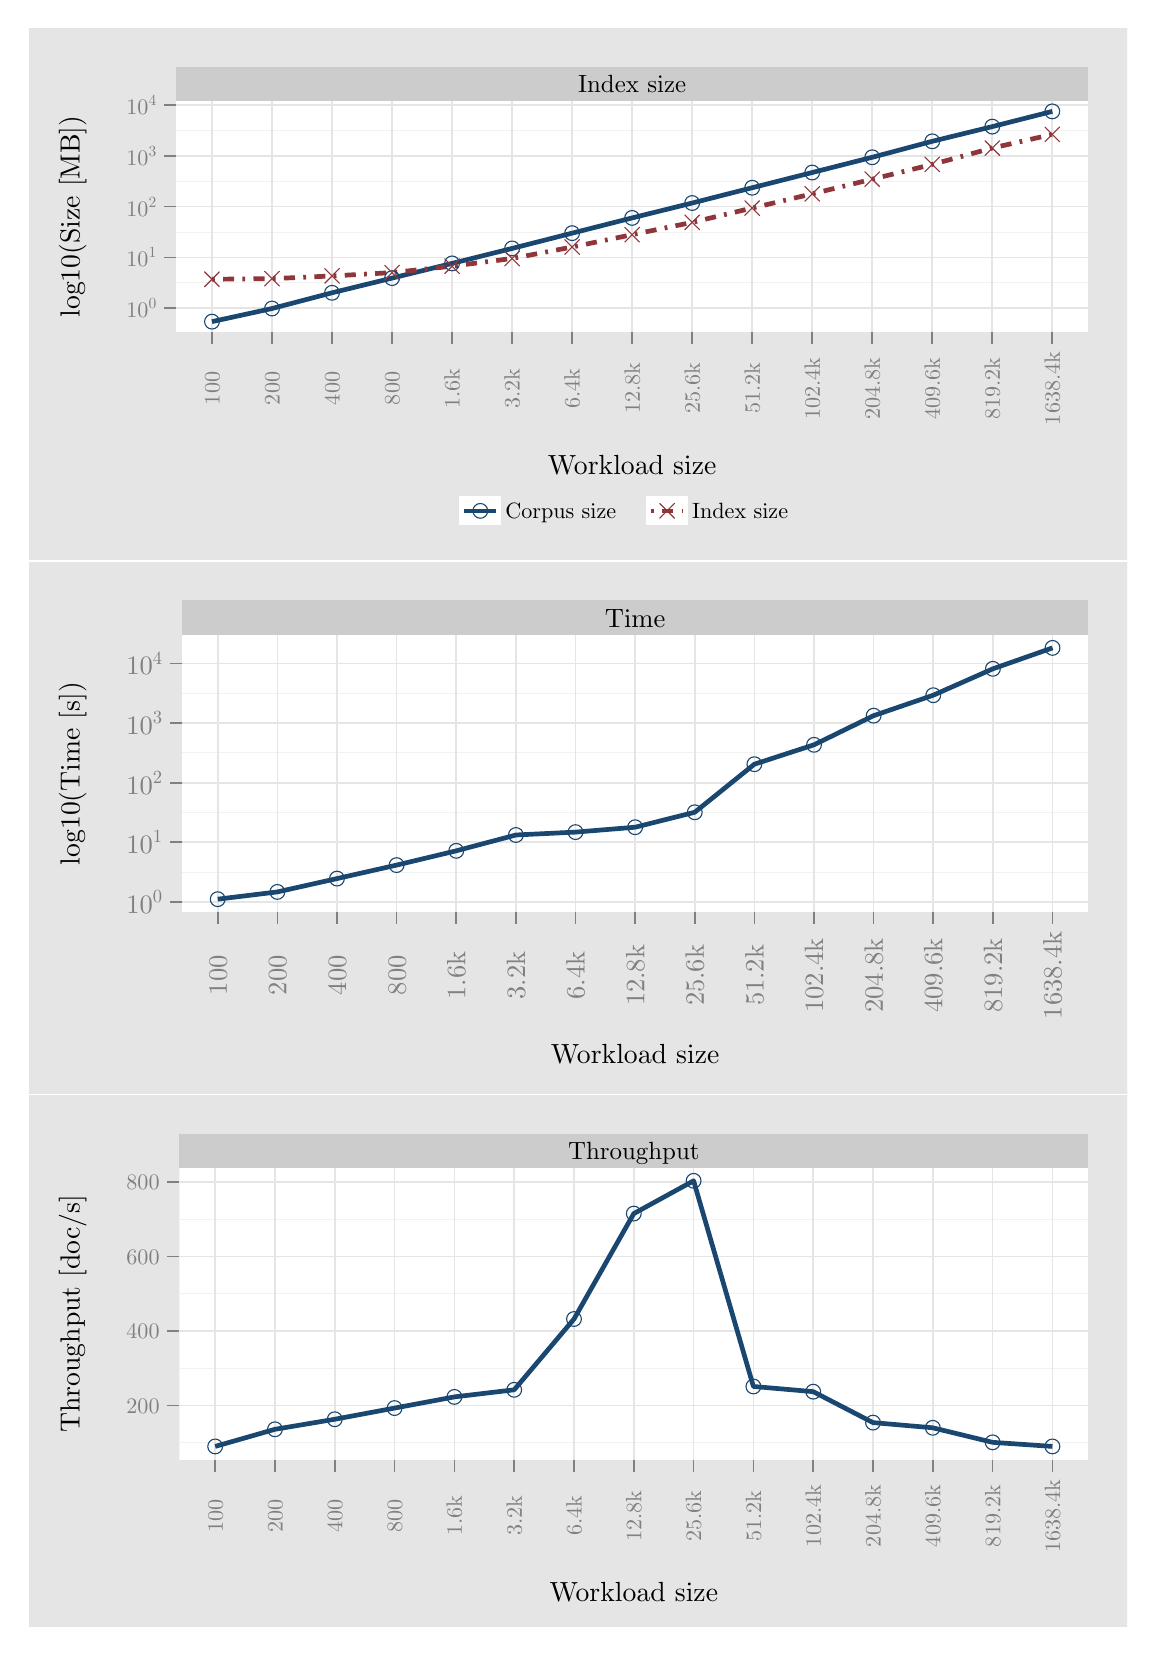
\begin{tikzpicture}[x=1pt,y=1pt]
\definecolor[named]{fillColor}{rgb}{1.00,1.00,1.00}
\path[use as bounding box,fill=fillColor,fill opacity=0.00] (0,0) rectangle (397.48,578.16);
\begin{scope}
\path[clip] (  0.00,385.44) rectangle (397.48,578.16);
\definecolor[named]{drawColor}{rgb}{1.00,1.00,1.00}
\definecolor[named]{fillColor}{rgb}{0.90,0.90,0.90}

\path[draw=drawColor,line width= 0.6pt,line join=round,line cap=round,fill=fillColor] (  0.00,385.44) rectangle (397.48,578.16);
\end{scope}
\begin{scope}
\path[clip] ( 53.58,468.13) rectangle (383.26,551.71);
\definecolor[named]{fillColor}{rgb}{1.00,1.00,1.00}

\path[fill=fillColor] ( 53.58,468.13) rectangle (383.26,551.71);
\definecolor[named]{drawColor}{rgb}{0.95,0.95,0.95}

\path[draw=drawColor,line width= 0.3pt,line join=round] ( 53.58,485.99) --
	(383.26,485.99);

\path[draw=drawColor,line width= 0.3pt,line join=round] ( 53.58,504.32) --
	(383.26,504.32);

\path[draw=drawColor,line width= 0.3pt,line join=round] ( 53.58,522.64) --
	(383.26,522.64);

\path[draw=drawColor,line width= 0.3pt,line join=round] ( 53.58,540.96) --
	(383.26,540.96);
\definecolor[named]{drawColor}{rgb}{0.90,0.90,0.90}

\path[draw=drawColor,line width= 0.6pt,line join=round] ( 53.58,476.83) --
	(383.26,476.83);

\path[draw=drawColor,line width= 0.6pt,line join=round] ( 53.58,495.15) --
	(383.26,495.15);

\path[draw=drawColor,line width= 0.6pt,line join=round] ( 53.58,513.48) --
	(383.26,513.48);

\path[draw=drawColor,line width= 0.6pt,line join=round] ( 53.58,531.80) --
	(383.26,531.80);

\path[draw=drawColor,line width= 0.6pt,line join=round] ( 53.58,550.12) --
	(383.26,550.12);

\path[draw=drawColor,line width= 0.6pt,line join=round] ( 66.60,468.13) --
	( 66.60,551.71);

\path[draw=drawColor,line width= 0.6pt,line join=round] ( 88.29,468.13) --
	( 88.29,551.71);

\path[draw=drawColor,line width= 0.6pt,line join=round] (109.97,468.13) --
	(109.97,551.71);

\path[draw=drawColor,line width= 0.6pt,line join=round] (131.66,468.13) --
	(131.66,551.71);

\path[draw=drawColor,line width= 0.6pt,line join=round] (153.35,468.13) --
	(153.35,551.71);

\path[draw=drawColor,line width= 0.6pt,line join=round] (175.04,468.13) --
	(175.04,551.71);

\path[draw=drawColor,line width= 0.6pt,line join=round] (196.73,468.13) --
	(196.73,551.71);

\path[draw=drawColor,line width= 0.6pt,line join=round] (218.42,468.13) --
	(218.42,551.71);

\path[draw=drawColor,line width= 0.6pt,line join=round] (240.11,468.13) --
	(240.11,551.71);

\path[draw=drawColor,line width= 0.6pt,line join=round] (261.80,468.13) --
	(261.80,551.71);

\path[draw=drawColor,line width= 0.6pt,line join=round] (283.49,468.13) --
	(283.49,551.71);

\path[draw=drawColor,line width= 0.6pt,line join=round] (305.18,468.13) --
	(305.18,551.71);

\path[draw=drawColor,line width= 0.6pt,line join=round] (326.87,468.13) --
	(326.87,551.71);

\path[draw=drawColor,line width= 0.6pt,line join=round] (348.56,468.13) --
	(348.56,551.71);

\path[draw=drawColor,line width= 0.6pt,line join=round] (370.25,468.13) --
	(370.25,551.71);
\definecolor[named]{drawColor}{rgb}{0.10,0.28,0.44}

\path[draw=drawColor,line width= 1.7pt,line join=round] ( 66.60,471.93) --
	( 88.29,476.67) --
	(109.97,482.35) --
	(131.66,487.66) --
	(153.35,492.97) --
	(175.04,498.38) --
	(196.73,503.90) --
	(218.42,509.41) --
	(240.11,514.79) --
	(261.80,520.31) --
	(283.49,525.81) --
	(305.18,531.32) --
	(326.87,537.09) --
	(348.56,542.40) --
	(370.25,547.91);
\definecolor[named]{drawColor}{rgb}{0.56,0.21,0.23}

\path[draw=drawColor,line width= 1.7pt,dash pattern=on 1pt off 3pt on 4pt off 3pt ,line join=round] ( 66.60,487.24) --
	( 88.29,487.46) --
	(109.97,488.44) --
	(131.66,489.64) --
	(153.35,491.97) --
	(175.04,494.75) --
	(196.73,498.89) --
	(218.42,503.35) --
	(240.11,507.80) --
	(261.80,512.98) --
	(283.49,518.11) --
	(305.18,523.40) --
	(326.87,528.73) --
	(348.56,534.66) --
	(370.25,539.59);
\definecolor[named]{drawColor}{rgb}{0.10,0.28,0.44}

\path[draw=drawColor,line width= 0.4pt,line join=round,line cap=round] ( 66.60,471.93) circle (  2.67);

\path[draw=drawColor,line width= 0.4pt,line join=round,line cap=round] ( 88.29,476.67) circle (  2.67);

\path[draw=drawColor,line width= 0.4pt,line join=round,line cap=round] (109.97,482.35) circle (  2.67);

\path[draw=drawColor,line width= 0.4pt,line join=round,line cap=round] (131.66,487.66) circle (  2.67);

\path[draw=drawColor,line width= 0.4pt,line join=round,line cap=round] (153.35,492.97) circle (  2.67);

\path[draw=drawColor,line width= 0.4pt,line join=round,line cap=round] (175.04,498.38) circle (  2.67);

\path[draw=drawColor,line width= 0.4pt,line join=round,line cap=round] (196.73,503.90) circle (  2.67);

\path[draw=drawColor,line width= 0.4pt,line join=round,line cap=round] (218.42,509.41) circle (  2.67);

\path[draw=drawColor,line width= 0.4pt,line join=round,line cap=round] (240.11,514.79) circle (  2.67);

\path[draw=drawColor,line width= 0.4pt,line join=round,line cap=round] (261.80,520.31) circle (  2.67);

\path[draw=drawColor,line width= 0.4pt,line join=round,line cap=round] (283.49,525.81) circle (  2.67);

\path[draw=drawColor,line width= 0.4pt,line join=round,line cap=round] (305.18,531.32) circle (  2.67);

\path[draw=drawColor,line width= 0.4pt,line join=round,line cap=round] (326.87,537.09) circle (  2.67);

\path[draw=drawColor,line width= 0.4pt,line join=round,line cap=round] (348.56,542.40) circle (  2.67);

\path[draw=drawColor,line width= 0.4pt,line join=round,line cap=round] (370.25,547.91) circle (  2.67);
\definecolor[named]{drawColor}{rgb}{0.56,0.21,0.23}

\path[draw=drawColor,line width= 0.4pt,line join=round,line cap=round,fill=fillColor] ( 63.93,484.58) -- ( 69.26,489.91);

\path[draw=drawColor,line width= 0.4pt,line join=round,line cap=round,fill=fillColor] ( 63.93,489.91) -- ( 69.26,484.58);

\path[draw=drawColor,line width= 0.4pt,line join=round,line cap=round,fill=fillColor] ( 85.62,484.79) -- ( 90.95,490.12);

\path[draw=drawColor,line width= 0.4pt,line join=round,line cap=round,fill=fillColor] ( 85.62,490.12) -- ( 90.95,484.79);

\path[draw=drawColor,line width= 0.4pt,line join=round,line cap=round,fill=fillColor] (107.31,485.77) -- (112.64,491.11);

\path[draw=drawColor,line width= 0.4pt,line join=round,line cap=round,fill=fillColor] (107.31,491.11) -- (112.64,485.77);

\path[draw=drawColor,line width= 0.4pt,line join=round,line cap=round,fill=fillColor] (129.00,486.97) -- (134.33,492.31);

\path[draw=drawColor,line width= 0.4pt,line join=round,line cap=round,fill=fillColor] (129.00,492.31) -- (134.33,486.97);

\path[draw=drawColor,line width= 0.4pt,line join=round,line cap=round,fill=fillColor] (150.69,489.30) -- (156.02,494.64);

\path[draw=drawColor,line width= 0.4pt,line join=round,line cap=round,fill=fillColor] (150.69,494.64) -- (156.02,489.30);

\path[draw=drawColor,line width= 0.4pt,line join=round,line cap=round,fill=fillColor] (172.37,492.08) -- (177.71,497.41);

\path[draw=drawColor,line width= 0.4pt,line join=round,line cap=round,fill=fillColor] (172.37,497.41) -- (177.71,492.08);

\path[draw=drawColor,line width= 0.4pt,line join=round,line cap=round,fill=fillColor] (194.06,496.23) -- (199.40,501.56);

\path[draw=drawColor,line width= 0.4pt,line join=round,line cap=round,fill=fillColor] (194.06,501.56) -- (199.40,496.23);

\path[draw=drawColor,line width= 0.4pt,line join=round,line cap=round,fill=fillColor] (215.75,500.68) -- (221.09,506.02);

\path[draw=drawColor,line width= 0.4pt,line join=round,line cap=round,fill=fillColor] (215.75,506.02) -- (221.09,500.68);

\path[draw=drawColor,line width= 0.4pt,line join=round,line cap=round,fill=fillColor] (237.44,505.13) -- (242.78,510.47);

\path[draw=drawColor,line width= 0.4pt,line join=round,line cap=round,fill=fillColor] (237.44,510.47) -- (242.78,505.13);

\path[draw=drawColor,line width= 0.4pt,line join=round,line cap=round,fill=fillColor] (259.13,510.32) -- (264.47,515.65);

\path[draw=drawColor,line width= 0.4pt,line join=round,line cap=round,fill=fillColor] (259.13,515.65) -- (264.47,510.32);

\path[draw=drawColor,line width= 0.4pt,line join=round,line cap=round,fill=fillColor] (280.82,515.44) -- (286.16,520.78);

\path[draw=drawColor,line width= 0.4pt,line join=round,line cap=round,fill=fillColor] (280.82,520.78) -- (286.16,515.44);

\path[draw=drawColor,line width= 0.4pt,line join=round,line cap=round,fill=fillColor] (302.51,520.73) -- (307.84,526.07);

\path[draw=drawColor,line width= 0.4pt,line join=round,line cap=round,fill=fillColor] (302.51,526.07) -- (307.84,520.73);

\path[draw=drawColor,line width= 0.4pt,line join=round,line cap=round,fill=fillColor] (324.20,526.06) -- (329.53,531.40);

\path[draw=drawColor,line width= 0.4pt,line join=round,line cap=round,fill=fillColor] (324.20,531.40) -- (329.53,526.06);

\path[draw=drawColor,line width= 0.4pt,line join=round,line cap=round,fill=fillColor] (345.89,532.00) -- (351.22,537.33);

\path[draw=drawColor,line width= 0.4pt,line join=round,line cap=round,fill=fillColor] (345.89,537.33) -- (351.22,532.00);

\path[draw=drawColor,line width= 0.4pt,line join=round,line cap=round,fill=fillColor] (367.58,536.92) -- (372.91,542.26);

\path[draw=drawColor,line width= 0.4pt,line join=round,line cap=round,fill=fillColor] (367.58,542.26) -- (372.91,536.92);
\end{scope}
\begin{scope}
\path[clip] (  0.00,  0.00) rectangle (397.48,578.16);
\definecolor[named]{fillColor}{rgb}{0.80,0.80,0.80}

\path[fill=fillColor] ( 53.58,551.71) rectangle (383.26,563.93);
\definecolor[named]{drawColor}{rgb}{0.00,0.00,0.00}

\node[text=drawColor,anchor=base,inner sep=0pt, outer sep=0pt, scale=  0.90] at (218.42,554.72) {Index size};
\end{scope}
\begin{scope}
\path[clip] (  0.00,  0.00) rectangle (397.48,578.16);
\definecolor[named]{drawColor}{rgb}{0.50,0.50,0.50}

\node[text=drawColor,anchor=base west,inner sep=0pt, outer sep=0pt, scale=  0.80] at ( 35.67,473.40) {10};

\node[text=drawColor,anchor=base west,inner sep=0pt, outer sep=0pt, scale=  0.56] at ( 43.67,476.67) {0};

\node[text=drawColor,anchor=base west,inner sep=0pt, outer sep=0pt, scale=  0.80] at ( 35.67,491.72) {10};

\node[text=drawColor,anchor=base west,inner sep=0pt, outer sep=0pt, scale=  0.56] at ( 43.67,494.99) {1};

\node[text=drawColor,anchor=base west,inner sep=0pt, outer sep=0pt, scale=  0.80] at ( 35.67,510.04) {10};

\node[text=drawColor,anchor=base west,inner sep=0pt, outer sep=0pt, scale=  0.56] at ( 43.67,513.32) {2};

\node[text=drawColor,anchor=base west,inner sep=0pt, outer sep=0pt, scale=  0.80] at ( 35.67,528.37) {10};

\node[text=drawColor,anchor=base west,inner sep=0pt, outer sep=0pt, scale=  0.56] at ( 43.67,531.64) {3};

\node[text=drawColor,anchor=base west,inner sep=0pt, outer sep=0pt, scale=  0.80] at ( 35.67,546.69) {10};

\node[text=drawColor,anchor=base west,inner sep=0pt, outer sep=0pt, scale=  0.56] at ( 43.67,549.96) {4};
\end{scope}
\begin{scope}
\path[clip] (  0.00,  0.00) rectangle (397.48,578.16);
\definecolor[named]{drawColor}{rgb}{0.50,0.50,0.50}

\path[draw=drawColor,line width= 0.6pt,line join=round] ( 49.31,476.83) --
	( 53.58,476.83);

\path[draw=drawColor,line width= 0.6pt,line join=round] ( 49.31,495.15) --
	( 53.58,495.15);

\path[draw=drawColor,line width= 0.6pt,line join=round] ( 49.31,513.48) --
	( 53.58,513.48);

\path[draw=drawColor,line width= 0.6pt,line join=round] ( 49.31,531.80) --
	( 53.58,531.80);

\path[draw=drawColor,line width= 0.6pt,line join=round] ( 49.31,550.12) --
	( 53.58,550.12);
\end{scope}
\begin{scope}
\path[clip] (  0.00,  0.00) rectangle (397.48,578.16);
\definecolor[named]{drawColor}{rgb}{0.50,0.50,0.50}

\path[draw=drawColor,line width= 0.6pt,line join=round] ( 66.60,463.86) --
	( 66.60,468.13);

\path[draw=drawColor,line width= 0.6pt,line join=round] ( 88.29,463.86) --
	( 88.29,468.13);

\path[draw=drawColor,line width= 0.6pt,line join=round] (109.97,463.86) --
	(109.97,468.13);

\path[draw=drawColor,line width= 0.6pt,line join=round] (131.66,463.86) --
	(131.66,468.13);

\path[draw=drawColor,line width= 0.6pt,line join=round] (153.35,463.86) --
	(153.35,468.13);

\path[draw=drawColor,line width= 0.6pt,line join=round] (175.04,463.86) --
	(175.04,468.13);

\path[draw=drawColor,line width= 0.6pt,line join=round] (196.73,463.86) --
	(196.73,468.13);

\path[draw=drawColor,line width= 0.6pt,line join=round] (218.42,463.86) --
	(218.42,468.13);

\path[draw=drawColor,line width= 0.6pt,line join=round] (240.11,463.86) --
	(240.11,468.13);

\path[draw=drawColor,line width= 0.6pt,line join=round] (261.80,463.86) --
	(261.80,468.13);

\path[draw=drawColor,line width= 0.6pt,line join=round] (283.49,463.86) --
	(283.49,468.13);

\path[draw=drawColor,line width= 0.6pt,line join=round] (305.18,463.86) --
	(305.18,468.13);

\path[draw=drawColor,line width= 0.6pt,line join=round] (326.87,463.86) --
	(326.87,468.13);

\path[draw=drawColor,line width= 0.6pt,line join=round] (348.56,463.86) --
	(348.56,468.13);

\path[draw=drawColor,line width= 0.6pt,line join=round] (370.25,463.86) --
	(370.25,468.13);
\end{scope}
\begin{scope}
\path[clip] (  0.00,  0.00) rectangle (397.48,578.16);
\definecolor[named]{drawColor}{rgb}{0.50,0.50,0.50}

\node[text=drawColor,rotate= 90.00,anchor=base,inner sep=0pt, outer sep=0pt, scale=  0.80] at ( 69.35,447.80) {100};

\node[text=drawColor,rotate= 90.00,anchor=base,inner sep=0pt, outer sep=0pt, scale=  0.80] at ( 91.04,447.80) {200};

\node[text=drawColor,rotate= 90.00,anchor=base,inner sep=0pt, outer sep=0pt, scale=  0.80] at (112.73,447.80) {400};

\node[text=drawColor,rotate= 90.00,anchor=base,inner sep=0pt, outer sep=0pt, scale=  0.80] at (134.42,447.80) {800};

\node[text=drawColor,rotate= 90.00,anchor=base,inner sep=0pt, outer sep=0pt, scale=  0.80] at (156.11,447.80) {1.6k};

\node[text=drawColor,rotate= 90.00,anchor=base,inner sep=0pt, outer sep=0pt, scale=  0.80] at (177.80,447.80) {3.2k};

\node[text=drawColor,rotate= 90.00,anchor=base,inner sep=0pt, outer sep=0pt, scale=  0.80] at (199.49,447.80) {6.4k};

\node[text=drawColor,rotate= 90.00,anchor=base,inner sep=0pt, outer sep=0pt, scale=  0.80] at (221.18,447.80) {12.8k};

\node[text=drawColor,rotate= 90.00,anchor=base,inner sep=0pt, outer sep=0pt, scale=  0.80] at (242.86,447.80) {25.6k};

\node[text=drawColor,rotate= 90.00,anchor=base,inner sep=0pt, outer sep=0pt, scale=  0.80] at (264.55,447.80) {51.2k};

\node[text=drawColor,rotate= 90.00,anchor=base,inner sep=0pt, outer sep=0pt, scale=  0.80] at (286.24,447.80) {102.4k};

\node[text=drawColor,rotate= 90.00,anchor=base,inner sep=0pt, outer sep=0pt, scale=  0.80] at (307.93,447.80) {204.8k};

\node[text=drawColor,rotate= 90.00,anchor=base,inner sep=0pt, outer sep=0pt, scale=  0.80] at (329.62,447.80) {409.6k};

\node[text=drawColor,rotate= 90.00,anchor=base,inner sep=0pt, outer sep=0pt, scale=  0.80] at (351.31,447.80) {819.2k};

\node[text=drawColor,rotate= 90.00,anchor=base,inner sep=0pt, outer sep=0pt, scale=  0.80] at (373.00,447.80) {1638.4k};
\end{scope}
\begin{scope}
\path[clip] (  0.00,  0.00) rectangle (397.48,578.16);
\definecolor[named]{drawColor}{rgb}{0.00,0.00,0.00}

\node[text=drawColor,anchor=base,inner sep=0pt, outer sep=0pt, scale=  1.00] at (218.42,416.85) {Workload size};
\end{scope}
\begin{scope}
\path[clip] (  0.00,  0.00) rectangle (397.48,578.16);
\definecolor[named]{drawColor}{rgb}{0.00,0.00,0.00}

\node[text=drawColor,rotate= 90.00,anchor=base,inner sep=0pt, outer sep=0pt, scale=  1.00] at ( 18.80,509.92) {log10(Size [MB])};
\end{scope}
\begin{scope}
\path[clip] (  0.00,  0.00) rectangle (397.48,578.16);
\definecolor[named]{fillColor}{rgb}{0.90,0.90,0.90}

\path[fill=fillColor] (148.45,394.31) rectangle (288.39,412.80);
\end{scope}
\begin{scope}
\path[clip] (  0.00,  0.00) rectangle (397.48,578.16);
\definecolor[named]{drawColor}{rgb}{1.00,1.00,1.00}
\definecolor[named]{fillColor}{rgb}{1.00,1.00,1.00}

\path[draw=drawColor,line width= 0.6pt,line join=round,line cap=round,fill=fillColor] (156.33,398.58) rectangle (170.78,408.53);
\end{scope}
\begin{scope}
\path[clip] (  0.00,  0.00) rectangle (397.48,578.16);
\definecolor[named]{drawColor}{rgb}{0.10,0.28,0.44}

\path[draw=drawColor,line width= 1.7pt,line join=round] (157.77,403.55) -- (169.34,403.55);
\end{scope}
\begin{scope}
\path[clip] (  0.00,  0.00) rectangle (397.48,578.16);
\definecolor[named]{drawColor}{rgb}{0.10,0.28,0.44}

\path[draw=drawColor,line width= 0.4pt,line join=round,line cap=round] (163.56,403.55) circle (  2.67);
\end{scope}
\begin{scope}
\path[clip] (  0.00,  0.00) rectangle (397.48,578.16);
\definecolor[named]{drawColor}{rgb}{1.00,1.00,1.00}
\definecolor[named]{fillColor}{rgb}{1.00,1.00,1.00}

\path[draw=drawColor,line width= 0.6pt,line join=round,line cap=round,fill=fillColor] (223.83,398.58) rectangle (238.28,408.53);
\end{scope}
\begin{scope}
\path[clip] (  0.00,  0.00) rectangle (397.48,578.16);
\definecolor[named]{drawColor}{rgb}{0.56,0.21,0.23}

\path[draw=drawColor,line width= 1.7pt,dash pattern=on 1pt off 3pt on 4pt off 3pt ,line join=round] (225.28,403.55) -- (236.84,403.55);
\end{scope}
\begin{scope}
\path[clip] (  0.00,  0.00) rectangle (397.48,578.16);
\definecolor[named]{drawColor}{rgb}{0.56,0.21,0.23}
\definecolor[named]{fillColor}{rgb}{1.00,1.00,1.00}

\path[draw=drawColor,line width= 0.4pt,line join=round,line cap=round,fill=fillColor] (228.39,400.89) -- (233.72,406.22);

\path[draw=drawColor,line width= 0.4pt,line join=round,line cap=round,fill=fillColor] (228.39,406.22) -- (233.72,400.89);
\end{scope}
\begin{scope}
\path[clip] (  0.00,  0.00) rectangle (397.48,578.16);
\definecolor[named]{drawColor}{rgb}{0.00,0.00,0.00}

\node[text=drawColor,anchor=base west,inner sep=0pt, outer sep=0pt, scale=  0.80] at (172.59,400.80) {Corpus size $\;\;\;$};
\end{scope}
\begin{scope}
\path[clip] (  0.00,  0.00) rectangle (397.48,578.16);
\definecolor[named]{drawColor}{rgb}{0.00,0.00,0.00}

\node[text=drawColor,anchor=base west,inner sep=0pt, outer sep=0pt, scale=  0.80] at (240.09,400.80) {Index size $\;\;\;$};
\end{scope}
\begin{scope}
\path[clip] (  0.00,192.72) rectangle (397.48,385.44);
\definecolor[named]{drawColor}{rgb}{1.00,1.00,1.00}
\definecolor[named]{fillColor}{rgb}{0.90,0.90,0.90}

\path[draw=drawColor,line width= 0.6pt,line join=round,line cap=round,fill=fillColor] (  0.00,192.72) rectangle (397.48,385.44);
\end{scope}
\begin{scope}
\path[clip] ( 55.74,258.70) rectangle (383.26,358.58);
\definecolor[named]{fillColor}{rgb}{1.00,1.00,1.00}

\path[fill=fillColor] ( 55.74,258.70) rectangle (383.26,358.58);
\definecolor[named]{drawColor}{rgb}{0.95,0.95,0.95}

\path[draw=drawColor,line width= 0.3pt,line join=round] ( 55.74,273.03) --
	(383.26,273.03);

\path[draw=drawColor,line width= 0.3pt,line join=round] ( 55.74,294.56) --
	(383.26,294.56);

\path[draw=drawColor,line width= 0.3pt,line join=round] ( 55.74,316.10) --
	(383.26,316.10);

\path[draw=drawColor,line width= 0.3pt,line join=round] ( 55.74,337.64) --
	(383.26,337.64);
\definecolor[named]{drawColor}{rgb}{0.90,0.90,0.90}

\path[draw=drawColor,line width= 0.6pt,line join=round] ( 55.74,262.26) --
	(383.26,262.26);

\path[draw=drawColor,line width= 0.6pt,line join=round] ( 55.74,283.80) --
	(383.26,283.80);

\path[draw=drawColor,line width= 0.6pt,line join=round] ( 55.74,305.33) --
	(383.26,305.33);

\path[draw=drawColor,line width= 0.6pt,line join=round] ( 55.74,326.87) --
	(383.26,326.87);

\path[draw=drawColor,line width= 0.6pt,line join=round] ( 55.74,348.41) --
	(383.26,348.41);

\path[draw=drawColor,line width= 0.6pt,line join=round] ( 68.67,258.70) --
	( 68.67,358.58);

\path[draw=drawColor,line width= 0.6pt,line join=round] ( 90.22,258.70) --
	( 90.22,358.58);

\path[draw=drawColor,line width= 0.6pt,line join=round] (111.76,258.70) --
	(111.76,358.58);

\path[draw=drawColor,line width= 0.6pt,line join=round] (133.31,258.70) --
	(133.31,358.58);

\path[draw=drawColor,line width= 0.6pt,line join=round] (154.86,258.70) --
	(154.86,358.58);

\path[draw=drawColor,line width= 0.6pt,line join=round] (176.41,258.70) --
	(176.41,358.58);

\path[draw=drawColor,line width= 0.6pt,line join=round] (197.95,258.70) --
	(197.95,358.58);

\path[draw=drawColor,line width= 0.6pt,line join=round] (219.50,258.70) --
	(219.50,358.58);

\path[draw=drawColor,line width= 0.6pt,line join=round] (241.05,258.70) --
	(241.05,358.58);

\path[draw=drawColor,line width= 0.6pt,line join=round] (262.59,258.70) --
	(262.59,358.58);

\path[draw=drawColor,line width= 0.6pt,line join=round] (284.14,258.70) --
	(284.14,358.58);

\path[draw=drawColor,line width= 0.6pt,line join=round] (305.69,258.70) --
	(305.69,358.58);

\path[draw=drawColor,line width= 0.6pt,line join=round] (327.24,258.70) --
	(327.24,358.58);

\path[draw=drawColor,line width= 0.6pt,line join=round] (348.78,258.70) --
	(348.78,358.58);

\path[draw=drawColor,line width= 0.6pt,line join=round] (370.33,258.70) --
	(370.33,358.58);
\definecolor[named]{drawColor}{rgb}{0.10,0.28,0.44}

\path[draw=drawColor,line width= 1.7pt,line join=round] ( 68.67,263.24) --
	( 90.22,265.86) --
	(111.76,270.68) --
	(133.31,275.55) --
	(154.86,280.71) --
	(176.41,286.43) --
	(197.95,287.47) --
	(219.50,289.24) --
	(241.05,294.64) --
	(262.59,312.01) --
	(284.14,319.02) --
	(305.69,329.55) --
	(327.24,336.94) --
	(348.78,346.48) --
	(370.33,354.04);

\path[draw=drawColor,line width= 0.4pt,line join=round,line cap=round] ( 68.67,263.24) circle (  2.67);

\path[draw=drawColor,line width= 0.4pt,line join=round,line cap=round] ( 90.22,265.86) circle (  2.67);

\path[draw=drawColor,line width= 0.4pt,line join=round,line cap=round] (111.76,270.68) circle (  2.67);

\path[draw=drawColor,line width= 0.4pt,line join=round,line cap=round] (133.31,275.55) circle (  2.67);

\path[draw=drawColor,line width= 0.4pt,line join=round,line cap=round] (154.86,280.71) circle (  2.67);

\path[draw=drawColor,line width= 0.4pt,line join=round,line cap=round] (176.41,286.43) circle (  2.67);

\path[draw=drawColor,line width= 0.4pt,line join=round,line cap=round] (197.95,287.47) circle (  2.67);

\path[draw=drawColor,line width= 0.4pt,line join=round,line cap=round] (219.50,289.24) circle (  2.67);

\path[draw=drawColor,line width= 0.4pt,line join=round,line cap=round] (241.05,294.64) circle (  2.67);

\path[draw=drawColor,line width= 0.4pt,line join=round,line cap=round] (262.59,312.01) circle (  2.67);

\path[draw=drawColor,line width= 0.4pt,line join=round,line cap=round] (284.14,319.02) circle (  2.67);

\path[draw=drawColor,line width= 0.4pt,line join=round,line cap=round] (305.69,329.55) circle (  2.67);

\path[draw=drawColor,line width= 0.4pt,line join=round,line cap=round] (327.24,336.94) circle (  2.67);

\path[draw=drawColor,line width= 0.4pt,line join=round,line cap=round] (348.78,346.48) circle (  2.67);

\path[draw=drawColor,line width= 0.4pt,line join=round,line cap=round] (370.33,354.04) circle (  2.67);
\end{scope}
\begin{scope}
\path[clip] (  0.00,  0.00) rectangle (397.48,578.16);
\definecolor[named]{fillColor}{rgb}{0.80,0.80,0.80}

\path[fill=fillColor] ( 55.74,358.58) rectangle (383.26,371.21);
\definecolor[named]{drawColor}{rgb}{0.00,0.00,0.00}

\node[text=drawColor,anchor=base,inner sep=0pt, outer sep=0pt, scale=  0.96] at (219.50,361.59) {Time};
\end{scope}
\begin{scope}
\path[clip] (  0.00,  0.00) rectangle (397.48,578.16);
\definecolor[named]{drawColor}{rgb}{0.50,0.50,0.50}

\node[text=drawColor,anchor=base west,inner sep=0pt, outer sep=0pt, scale=  0.96] at ( 35.67,258.14) {10};

\node[text=drawColor,anchor=base west,inner sep=0pt, outer sep=0pt, scale=  0.67] at ( 45.27,262.07) {0};

\node[text=drawColor,anchor=base west,inner sep=0pt, outer sep=0pt, scale=  0.96] at ( 35.67,279.68) {10};

\node[text=drawColor,anchor=base west,inner sep=0pt, outer sep=0pt, scale=  0.67] at ( 45.27,283.60) {1};

\node[text=drawColor,anchor=base west,inner sep=0pt, outer sep=0pt, scale=  0.96] at ( 35.67,301.21) {10};

\node[text=drawColor,anchor=base west,inner sep=0pt, outer sep=0pt, scale=  0.67] at ( 45.27,305.14) {2};

\node[text=drawColor,anchor=base west,inner sep=0pt, outer sep=0pt, scale=  0.96] at ( 35.67,322.75) {10};

\node[text=drawColor,anchor=base west,inner sep=0pt, outer sep=0pt, scale=  0.67] at ( 45.27,326.68) {3};

\node[text=drawColor,anchor=base west,inner sep=0pt, outer sep=0pt, scale=  0.96] at ( 35.67,344.29) {10};

\node[text=drawColor,anchor=base west,inner sep=0pt, outer sep=0pt, scale=  0.67] at ( 45.27,348.21) {4};
\end{scope}
\begin{scope}
\path[clip] (  0.00,  0.00) rectangle (397.48,578.16);
\definecolor[named]{drawColor}{rgb}{0.50,0.50,0.50}

\path[draw=drawColor,line width= 0.6pt,line join=round] ( 51.47,262.26) --
	( 55.74,262.26);

\path[draw=drawColor,line width= 0.6pt,line join=round] ( 51.47,283.80) --
	( 55.74,283.80);

\path[draw=drawColor,line width= 0.6pt,line join=round] ( 51.47,305.33) --
	( 55.74,305.33);

\path[draw=drawColor,line width= 0.6pt,line join=round] ( 51.47,326.87) --
	( 55.74,326.87);

\path[draw=drawColor,line width= 0.6pt,line join=round] ( 51.47,348.41) --
	( 55.74,348.41);
\end{scope}
\begin{scope}
\path[clip] (  0.00,  0.00) rectangle (397.48,578.16);
\definecolor[named]{drawColor}{rgb}{0.50,0.50,0.50}

\path[draw=drawColor,line width= 0.6pt,line join=round] ( 68.67,254.43) --
	( 68.67,258.70);

\path[draw=drawColor,line width= 0.6pt,line join=round] ( 90.22,254.43) --
	( 90.22,258.70);

\path[draw=drawColor,line width= 0.6pt,line join=round] (111.76,254.43) --
	(111.76,258.70);

\path[draw=drawColor,line width= 0.6pt,line join=round] (133.31,254.43) --
	(133.31,258.70);

\path[draw=drawColor,line width= 0.6pt,line join=round] (154.86,254.43) --
	(154.86,258.70);

\path[draw=drawColor,line width= 0.6pt,line join=round] (176.41,254.43) --
	(176.41,258.70);

\path[draw=drawColor,line width= 0.6pt,line join=round] (197.95,254.43) --
	(197.95,258.70);

\path[draw=drawColor,line width= 0.6pt,line join=round] (219.50,254.43) --
	(219.50,258.70);

\path[draw=drawColor,line width= 0.6pt,line join=round] (241.05,254.43) --
	(241.05,258.70);

\path[draw=drawColor,line width= 0.6pt,line join=round] (262.59,254.43) --
	(262.59,258.70);

\path[draw=drawColor,line width= 0.6pt,line join=round] (284.14,254.43) --
	(284.14,258.70);

\path[draw=drawColor,line width= 0.6pt,line join=round] (305.69,254.43) --
	(305.69,258.70);

\path[draw=drawColor,line width= 0.6pt,line join=round] (327.24,254.43) --
	(327.24,258.70);

\path[draw=drawColor,line width= 0.6pt,line join=round] (348.78,254.43) --
	(348.78,258.70);

\path[draw=drawColor,line width= 0.6pt,line join=round] (370.33,254.43) --
	(370.33,258.70);
\end{scope}
\begin{scope}
\path[clip] (  0.00,  0.00) rectangle (397.48,578.16);
\definecolor[named]{drawColor}{rgb}{0.50,0.50,0.50}

\node[text=drawColor,rotate= 90.00,anchor=base,inner sep=0pt, outer sep=0pt, scale=  0.96] at ( 71.98,235.72) {100};

\node[text=drawColor,rotate= 90.00,anchor=base,inner sep=0pt, outer sep=0pt, scale=  0.96] at ( 93.52,235.72) {200};

\node[text=drawColor,rotate= 90.00,anchor=base,inner sep=0pt, outer sep=0pt, scale=  0.96] at (115.07,235.72) {400};

\node[text=drawColor,rotate= 90.00,anchor=base,inner sep=0pt, outer sep=0pt, scale=  0.96] at (136.62,235.72) {800};

\node[text=drawColor,rotate= 90.00,anchor=base,inner sep=0pt, outer sep=0pt, scale=  0.96] at (158.16,235.72) {1.6k};

\node[text=drawColor,rotate= 90.00,anchor=base,inner sep=0pt, outer sep=0pt, scale=  0.96] at (179.71,235.72) {3.2k};

\node[text=drawColor,rotate= 90.00,anchor=base,inner sep=0pt, outer sep=0pt, scale=  0.96] at (201.26,235.72) {6.4k};

\node[text=drawColor,rotate= 90.00,anchor=base,inner sep=0pt, outer sep=0pt, scale=  0.96] at (222.81,235.72) {12.8k};

\node[text=drawColor,rotate= 90.00,anchor=base,inner sep=0pt, outer sep=0pt, scale=  0.96] at (244.35,235.72) {25.6k};

\node[text=drawColor,rotate= 90.00,anchor=base,inner sep=0pt, outer sep=0pt, scale=  0.96] at (265.90,235.72) {51.2k};

\node[text=drawColor,rotate= 90.00,anchor=base,inner sep=0pt, outer sep=0pt, scale=  0.96] at (287.45,235.72) {102.4k};

\node[text=drawColor,rotate= 90.00,anchor=base,inner sep=0pt, outer sep=0pt, scale=  0.96] at (308.99,235.72) {204.8k};

\node[text=drawColor,rotate= 90.00,anchor=base,inner sep=0pt, outer sep=0pt, scale=  0.96] at (330.54,235.72) {409.6k};

\node[text=drawColor,rotate= 90.00,anchor=base,inner sep=0pt, outer sep=0pt, scale=  0.96] at (352.09,235.72) {819.2k};

\node[text=drawColor,rotate= 90.00,anchor=base,inner sep=0pt, outer sep=0pt, scale=  0.96] at (373.64,235.72) {1638.4k};
\end{scope}
\begin{scope}
\path[clip] (  0.00,  0.00) rectangle (397.48,578.16);
\definecolor[named]{drawColor}{rgb}{0.00,0.00,0.00}

\node[text=drawColor,anchor=base,inner sep=0pt, outer sep=0pt, scale=  1.00] at (219.50,203.94) {Workload size};
\end{scope}
\begin{scope}
\path[clip] (  0.00,  0.00) rectangle (397.48,578.16);
\definecolor[named]{drawColor}{rgb}{0.00,0.00,0.00}

\node[text=drawColor,rotate= 90.00,anchor=base,inner sep=0pt, outer sep=0pt, scale=  1.00] at ( 18.80,308.64) {log10(Time [s])};
\end{scope}
\begin{scope}
\path[clip] (  0.00,  0.00) rectangle (397.48,192.72);
\definecolor[named]{drawColor}{rgb}{1.00,1.00,1.00}
\definecolor[named]{fillColor}{rgb}{0.90,0.90,0.90}

\path[draw=drawColor,line width= 0.6pt,line join=round,line cap=round,fill=fillColor] (  0.00,  0.00) rectangle (397.48,192.72);
\end{scope}
\begin{scope}
\path[clip] ( 54.78, 60.69) rectangle (383.26,166.27);
\definecolor[named]{fillColor}{rgb}{1.00,1.00,1.00}

\path[fill=fillColor] ( 54.78, 60.69) rectangle (383.26,166.27);
\definecolor[named]{drawColor}{rgb}{0.95,0.95,0.95}

\path[draw=drawColor,line width= 0.3pt,line join=round] ( 54.78, 66.83) --
	(383.26, 66.83);

\path[draw=drawColor,line width= 0.3pt,line join=round] ( 54.78, 93.76) --
	(383.26, 93.76);

\path[draw=drawColor,line width= 0.3pt,line join=round] ( 54.78,120.68) --
	(383.26,120.68);

\path[draw=drawColor,line width= 0.3pt,line join=round] ( 54.78,147.61) --
	(383.26,147.61);
\definecolor[named]{drawColor}{rgb}{0.90,0.90,0.90}

\path[draw=drawColor,line width= 0.6pt,line join=round] ( 54.78, 80.30) --
	(383.26, 80.30);

\path[draw=drawColor,line width= 0.6pt,line join=round] ( 54.78,107.22) --
	(383.26,107.22);

\path[draw=drawColor,line width= 0.6pt,line join=round] ( 54.78,134.14) --
	(383.26,134.14);

\path[draw=drawColor,line width= 0.6pt,line join=round] ( 54.78,161.07) --
	(383.26,161.07);

\path[draw=drawColor,line width= 0.6pt,line join=round] ( 67.75, 60.69) --
	( 67.75,166.27);

\path[draw=drawColor,line width= 0.6pt,line join=round] ( 89.36, 60.69) --
	( 89.36,166.27);

\path[draw=drawColor,line width= 0.6pt,line join=round] (110.97, 60.69) --
	(110.97,166.27);

\path[draw=drawColor,line width= 0.6pt,line join=round] (132.58, 60.69) --
	(132.58,166.27);

\path[draw=drawColor,line width= 0.6pt,line join=round] (154.19, 60.69) --
	(154.19,166.27);

\path[draw=drawColor,line width= 0.6pt,line join=round] (175.80, 60.69) --
	(175.80,166.27);

\path[draw=drawColor,line width= 0.6pt,line join=round] (197.41, 60.69) --
	(197.41,166.27);

\path[draw=drawColor,line width= 0.6pt,line join=round] (219.02, 60.69) --
	(219.02,166.27);

\path[draw=drawColor,line width= 0.6pt,line join=round] (240.63, 60.69) --
	(240.63,166.27);

\path[draw=drawColor,line width= 0.6pt,line join=round] (262.24, 60.69) --
	(262.24,166.27);

\path[draw=drawColor,line width= 0.6pt,line join=round] (283.85, 60.69) --
	(283.85,166.27);

\path[draw=drawColor,line width= 0.6pt,line join=round] (305.46, 60.69) --
	(305.46,166.27);

\path[draw=drawColor,line width= 0.6pt,line join=round] (327.07, 60.69) --
	(327.07,166.27);

\path[draw=drawColor,line width= 0.6pt,line join=round] (348.68, 60.69) --
	(348.68,166.27);

\path[draw=drawColor,line width= 0.6pt,line join=round] (370.29, 60.69) --
	(370.29,166.27);
\definecolor[named]{drawColor}{rgb}{0.10,0.28,0.44}

\path[draw=drawColor,line width= 1.7pt,line join=round] ( 67.75, 65.49) --
	( 89.36, 71.68) --
	(110.97, 75.31) --
	(132.58, 79.35) --
	(154.19, 83.39) --
	(175.80, 85.95) --
	(197.41,111.53) --
	(219.02,149.63) --
	(240.63,161.47) --
	(262.24, 87.16) --
	(283.85, 85.28) --
	(305.46, 74.10) --
	(327.07, 72.22) --
	(348.68, 66.97) --
	(370.29, 65.49);

\path[draw=drawColor,line width= 0.4pt,line join=round,line cap=round] ( 67.75, 65.49) circle (  2.67);

\path[draw=drawColor,line width= 0.4pt,line join=round,line cap=round] ( 89.36, 71.68) circle (  2.67);

\path[draw=drawColor,line width= 0.4pt,line join=round,line cap=round] (110.97, 75.31) circle (  2.67);

\path[draw=drawColor,line width= 0.4pt,line join=round,line cap=round] (132.58, 79.35) circle (  2.67);

\path[draw=drawColor,line width= 0.4pt,line join=round,line cap=round] (154.19, 83.39) circle (  2.67);

\path[draw=drawColor,line width= 0.4pt,line join=round,line cap=round] (175.80, 85.95) circle (  2.67);

\path[draw=drawColor,line width= 0.4pt,line join=round,line cap=round] (197.41,111.53) circle (  2.67);

\path[draw=drawColor,line width= 0.4pt,line join=round,line cap=round] (219.02,149.63) circle (  2.67);

\path[draw=drawColor,line width= 0.4pt,line join=round,line cap=round] (240.63,161.47) circle (  2.67);

\path[draw=drawColor,line width= 0.4pt,line join=round,line cap=round] (262.24, 87.16) circle (  2.67);

\path[draw=drawColor,line width= 0.4pt,line join=round,line cap=round] (283.85, 85.28) circle (  2.67);

\path[draw=drawColor,line width= 0.4pt,line join=round,line cap=round] (305.46, 74.10) circle (  2.67);

\path[draw=drawColor,line width= 0.4pt,line join=round,line cap=round] (327.07, 72.22) circle (  2.67);

\path[draw=drawColor,line width= 0.4pt,line join=round,line cap=round] (348.68, 66.97) circle (  2.67);

\path[draw=drawColor,line width= 0.4pt,line join=round,line cap=round] (370.29, 65.49) circle (  2.67);
\end{scope}
\begin{scope}
\path[clip] (  0.00,  0.00) rectangle (397.48,578.16);
\definecolor[named]{fillColor}{rgb}{0.80,0.80,0.80}

\path[fill=fillColor] ( 54.78,166.27) rectangle (383.26,178.49);
\definecolor[named]{drawColor}{rgb}{0.00,0.00,0.00}

\node[text=drawColor,anchor=base,inner sep=0pt, outer sep=0pt, scale=  0.90] at (219.02,169.28) {Throughput};
\end{scope}
\begin{scope}
\path[clip] (  0.00,  0.00) rectangle (397.48,578.16);
\definecolor[named]{drawColor}{rgb}{0.50,0.50,0.50}

\node[text=drawColor,anchor=base east,inner sep=0pt, outer sep=0pt, scale=  0.80] at ( 47.67, 77.54) {200};

\node[text=drawColor,anchor=base east,inner sep=0pt, outer sep=0pt, scale=  0.80] at ( 47.67,104.47) {400};

\node[text=drawColor,anchor=base east,inner sep=0pt, outer sep=0pt, scale=  0.80] at ( 47.67,131.39) {600};

\node[text=drawColor,anchor=base east,inner sep=0pt, outer sep=0pt, scale=  0.80] at ( 47.67,158.31) {800};
\end{scope}
\begin{scope}
\path[clip] (  0.00,  0.00) rectangle (397.48,578.16);
\definecolor[named]{drawColor}{rgb}{0.50,0.50,0.50}

\path[draw=drawColor,line width= 0.6pt,line join=round] ( 50.51, 80.30) --
	( 54.78, 80.30);

\path[draw=drawColor,line width= 0.6pt,line join=round] ( 50.51,107.22) --
	( 54.78,107.22);

\path[draw=drawColor,line width= 0.6pt,line join=round] ( 50.51,134.14) --
	( 54.78,134.14);

\path[draw=drawColor,line width= 0.6pt,line join=round] ( 50.51,161.07) --
	( 54.78,161.07);
\end{scope}
\begin{scope}
\path[clip] (  0.00,  0.00) rectangle (397.48,578.16);
\definecolor[named]{drawColor}{rgb}{0.50,0.50,0.50}

\path[draw=drawColor,line width= 0.6pt,line join=round] ( 67.75, 56.42) --
	( 67.75, 60.69);

\path[draw=drawColor,line width= 0.6pt,line join=round] ( 89.36, 56.42) --
	( 89.36, 60.69);

\path[draw=drawColor,line width= 0.6pt,line join=round] (110.97, 56.42) --
	(110.97, 60.69);

\path[draw=drawColor,line width= 0.6pt,line join=round] (132.58, 56.42) --
	(132.58, 60.69);

\path[draw=drawColor,line width= 0.6pt,line join=round] (154.19, 56.42) --
	(154.19, 60.69);

\path[draw=drawColor,line width= 0.6pt,line join=round] (175.80, 56.42) --
	(175.80, 60.69);

\path[draw=drawColor,line width= 0.6pt,line join=round] (197.41, 56.42) --
	(197.41, 60.69);

\path[draw=drawColor,line width= 0.6pt,line join=round] (219.02, 56.42) --
	(219.02, 60.69);

\path[draw=drawColor,line width= 0.6pt,line join=round] (240.63, 56.42) --
	(240.63, 60.69);

\path[draw=drawColor,line width= 0.6pt,line join=round] (262.24, 56.42) --
	(262.24, 60.69);

\path[draw=drawColor,line width= 0.6pt,line join=round] (283.85, 56.42) --
	(283.85, 60.69);

\path[draw=drawColor,line width= 0.6pt,line join=round] (305.46, 56.42) --
	(305.46, 60.69);

\path[draw=drawColor,line width= 0.6pt,line join=round] (327.07, 56.42) --
	(327.07, 60.69);

\path[draw=drawColor,line width= 0.6pt,line join=round] (348.68, 56.42) --
	(348.68, 60.69);

\path[draw=drawColor,line width= 0.6pt,line join=round] (370.29, 56.42) --
	(370.29, 60.69);
\end{scope}
\begin{scope}
\path[clip] (  0.00,  0.00) rectangle (397.48,578.16);
\definecolor[named]{drawColor}{rgb}{0.50,0.50,0.50}

\node[text=drawColor,rotate= 90.00,anchor=base,inner sep=0pt, outer sep=0pt, scale=  0.80] at ( 70.50, 40.36) {100};

\node[text=drawColor,rotate= 90.00,anchor=base,inner sep=0pt, outer sep=0pt, scale=  0.80] at ( 92.11, 40.36) {200};

\node[text=drawColor,rotate= 90.00,anchor=base,inner sep=0pt, outer sep=0pt, scale=  0.80] at (113.72, 40.36) {400};

\node[text=drawColor,rotate= 90.00,anchor=base,inner sep=0pt, outer sep=0pt, scale=  0.80] at (135.33, 40.36) {800};

\node[text=drawColor,rotate= 90.00,anchor=base,inner sep=0pt, outer sep=0pt, scale=  0.80] at (156.94, 40.36) {1.6k};

\node[text=drawColor,rotate= 90.00,anchor=base,inner sep=0pt, outer sep=0pt, scale=  0.80] at (178.55, 40.36) {3.2k};

\node[text=drawColor,rotate= 90.00,anchor=base,inner sep=0pt, outer sep=0pt, scale=  0.80] at (200.17, 40.36) {6.4k};

\node[text=drawColor,rotate= 90.00,anchor=base,inner sep=0pt, outer sep=0pt, scale=  0.80] at (221.78, 40.36) {12.8k};

\node[text=drawColor,rotate= 90.00,anchor=base,inner sep=0pt, outer sep=0pt, scale=  0.80] at (243.39, 40.36) {25.6k};

\node[text=drawColor,rotate= 90.00,anchor=base,inner sep=0pt, outer sep=0pt, scale=  0.80] at (265.00, 40.36) {51.2k};

\node[text=drawColor,rotate= 90.00,anchor=base,inner sep=0pt, outer sep=0pt, scale=  0.80] at (286.61, 40.36) {102.4k};

\node[text=drawColor,rotate= 90.00,anchor=base,inner sep=0pt, outer sep=0pt, scale=  0.80] at (308.22, 40.36) {204.8k};

\node[text=drawColor,rotate= 90.00,anchor=base,inner sep=0pt, outer sep=0pt, scale=  0.80] at (329.83, 40.36) {409.6k};

\node[text=drawColor,rotate= 90.00,anchor=base,inner sep=0pt, outer sep=0pt, scale=  0.80] at (351.44, 40.36) {819.2k};

\node[text=drawColor,rotate= 90.00,anchor=base,inner sep=0pt, outer sep=0pt, scale=  0.80] at (373.05, 40.36) {1638.4k};
\end{scope}
\begin{scope}
\path[clip] (  0.00,  0.00) rectangle (397.48,578.16);
\definecolor[named]{drawColor}{rgb}{0.00,0.00,0.00}

\node[text=drawColor,anchor=base,inner sep=0pt, outer sep=0pt, scale=  1.00] at (219.02,  9.41) {Workload size};
\end{scope}
\begin{scope}
\path[clip] (  0.00,  0.00) rectangle (397.48,578.16);
\definecolor[named]{drawColor}{rgb}{0.00,0.00,0.00}

\node[text=drawColor,rotate= 90.00,anchor=base,inner sep=0pt, outer sep=0pt, scale=  1.00] at ( 18.80,113.48) {Throughput [doc/s]};
\end{scope}
\end{tikzpicture}

 }
 \caption[Baseline performance benchmarks for batch indexing]{Indexing operations performance benchmarks results showing the size of the indices on disk, the time taken to generate the indices, and the indexing\index{Index} process throughput. Notice how the throughput plummets when the workload\index{Workload} goes beyond \num{25600} documents.}
 \label{fig:experimentation:performance:indexing:index-throughput}
\end{figure}

\tablespacing
%\begin{longtable} {p{0.20\linewidth} S[table-format=1.4]p{0.20\linewidth}
%S[table-format=1.4]p{0.20\linewidth} S[table-format=1.4]p{0.30\linewidth}}

%%%%%\begin{longtable} {
%%%%%p{0.10\linewidth} 
%%%%%S[table-format=1.4]
%%%%%S[table-format=1.4] 
%%%%%S[table-format=1.4]}
\begin{longtable}{
>{\arraybackslash}m{0.07\linewidth}|
>{\centering\arraybackslash}m{0.18\linewidth}|
>{\centering\arraybackslash}m{0.18\linewidth}|
>{\centering\arraybackslash}m{0.28\linewidth}
}
 
 \caption{Baseline performance benchmarks for batch indexing}
\label{tab:experimentation:performance:indexing:batch-indexing} \\
 %%%%%\toprule
 \hline
 %%{} & 
 %%\textbf{\pbox{20cm}{Index \\(MB)}} &
 %%{} & 
 %%\textbf{\pbox{20cm}{Time \\(secs)}} &
 %%{} &
 %%\textbf{\pbox{20cm}{Throughput\\(docs/sec)}} \\
  {} & 
 \textbf{Index [MB]} &
 %%{} & 
 \textbf{Time [s]} &
 %%{} &
 \textbf{Throughput [doc/s]} \\
 %%%%%\midrule
 \hline \hline
 \endfirsthead
 
 \caption[]{(continued)}\\
 %%%%%\toprule
 \hline
 %%{} & 
 %%\textbf{\pbox{20cm}{Index \\(MB)}} &
 %%{} & 
 %%\textbf{\pbox{20cm}{Time \\(secs)}} &
 %%{} &
 %%\textbf{\pbox{20cm}{Throughput\\(docs/sec)}} \\
  {} & 
 \textbf{Index [MB]} &
 %%{} & 
 \textbf{Time [s]} &
 %%{} &
 \textbf{Throughput [doc/s]} \\
 %%%%%\midrule
 \hline \hline
 \endhead
 
 % Page footer
 %%%%%\midrule
 \hline
 \multicolumn{4}{r}{(Continued on next page)} \\
 \endfoot
 
 % Last page footer
 \bottomrule
 \endlastfoot

 %W1&
 \textbf{W1}&
 {\tablenum[table-format=4.2]{0.40}}&
 %%{}&
 {\tablenum[table-format=4.2]{1.11}}&
 %%{}&
 {\tablenum[table-format=4]{90}}\\

 %\cmidrule[0.1pt](l{0.5em}r{0.5em}){1-2}

 %W2&
 \textbf{W2}&
 {\tablenum[table-format=4.2]{0.56}}&
 %%{}&
 {\tablenum[table-format=4.2]{1.47}}&
 %%{}&
 {\tablenum[table-format=4]{136}}\\

 %\cmidrule[0.1pt](l{0.5em}r{0.5em}){1-2}
 
 %W3&
 \textbf{W3}&
 {\tablenum[table-format=4.2]{1.10}}&
 %%{}&
 {\tablenum[table-format=4.2]{2.46}}&
 %%{}&
 {\tablenum[table-format=4]{163}}\\

 %\cmidrule[0.1pt](l{0.5em}r{0.5em}){1-2}
 
 %W4&
 \textbf{W4}&
 {\tablenum[table-format=4.2]{1.90}}&
 %%{}&
 {\tablenum[table-format=4.2]{4.14}}&
 %%{}&
 {\tablenum[table-format=4]{193}}\\

 %\cmidrule[0.1pt](l{0.5em}r{0.5em}){1-2}
 
 %W5&
 \textbf{W5}&
 {\tablenum[table-format=4.2]{3.50}}&
 %%{}&
 {\tablenum[table-format=4.2]{7.19}}&
 %%{}&
 {\tablenum[table-format=4]{223}}\\

 %\cmidrule[0.1pt](l{0.5em}r{0.5em}){1-2}
 
 %W6&
 \textbf{W6}&
 {\tablenum[table-format=4.2]{6.40}}&
 %%{}&
 {\tablenum[table-format=4.2]{13.25}}&
 %%{}&
 {\tablenum[table-format=4]{242}}\\

 %\cmidrule[0.1pt](l{0.5em}r{0.5em}){1-2}
 
 %W7&
 \textbf{W7}&
 {\tablenum[table-format=4.2]{12.00}}&
 %%{}&
 {\tablenum[table-format=4.2]{14.81}}&
 %%{}&
 {\tablenum[table-format=4]{432}}\\

 %\cmidrule[0.1pt](l{0.5em}r{0.5em}){1-2}
 
 %W8&
 \textbf{W8}&
 {\tablenum[table-format=4.2]{24.00}}&
 %%{}&
 {\tablenum[table-format=4.2]{17.89}}&
 %%{}&
 {\tablenum[table-format=4]{715}}\\

 %\cmidrule[0.1pt](l{0.5em}r{0.5em}){1-2}
 
 %W9&
 \textbf{W9}&
 {\tablenum[table-format=4.2]{46.00}}&
 %%{}&
 {\tablenum[table-format=4.2]{31.87}}&
 %%{}&
 {\tablenum[table-format=4]{803}}\\

 %\cmidrule[0.1pt](l{0.5em}r{0.5em}){1-2}
 
 %W10&
 \textbf{W10}&
 {\tablenum[table-format=4.2]{91.00}}&
 %%{}&
 {\tablenum[table-format=4.2]{204.21}}&
 %%{}&
 {\tablenum[table-format=4]{251}}\\

 %\cmidrule[0.1pt](l{0.5em}r{0.5em}){1-2}
 
 %W11&
 \textbf{W11}&
 {\tablenum[table-format=4.2]{179.00}}&
 %%{}&
 {\tablenum[table-format=4.2]{432.12}}&
 %%{}&
 {\tablenum[table-format=4]{237}}\\

 %\cmidrule[0.1pt](l{0.5em}r{0.5em}){1-2}
 
 %W12&
 \textbf{W12}&
 {\tablenum[table-format=4.2]{348.00}}&
 %%{}&
 {\tablenum[table-format=4.2]{1331.99}}&
 %%{}&
 {\tablenum[table-format=4]{154}}\\

 %\cmidrule[0.1pt](l{0.5em}r{0.5em}){1-2}
 
 %W13&
 \textbf{W13}&
 {\tablenum[table-format=4.2]{962.00}}&
 %%{}&
 {\tablenum[table-format=4.2]{2934.96}}&
 %%{}&
 {\tablenum[table-format=4]{140}}\\

 %\cmidrule[0.1pt](l{0.5em}r{0.5em}){1-2}
 
 %W14&
 \textbf{W14}&
 {\tablenum[table-format=4.2]{1433.60}}&
 %%{}&
 {\tablenum[table-format=4.2]{8134.99}}&
 %%{}&
 {\tablenum[table-format=4]{101}}\\

 %\cmidrule[0.1pt](l{0.5em}r{0.5em}){1-2}
 
 %W15&
 \textbf{W15}&
 {\tablenum[table-format=4.2]{2662.40}}&
 %%{}&
 {\tablenum[table-format=4.2]{18261.88}}&
 %%{}&
 {\tablenum[table-format=4]{90}}\\

 %\cmidrule[0.1pt](l{0.5em}r{0.5em}){1-2}

\end{longtable}

\bodyspacing

\paragraph{Experiment: Incremental collection indexing\index{Index} benchmarks}
\label{sec:evaluation:performance:indexing:experiment2}

This experiment was conducted to assess the performance of the indexing\index{Index} process, relative to the size of the collection, when collections are updated with new content.

\subparagraph{Methodology}

A batch of \num{1000} latest records\footnote{OAI-PMH 'from' parameter was used to harvest records not previously harvested} were harvested from the NDLTD portal and added to existing workload\index{Workload} indices using Apache Solr XSLT UpdateRequestHandler \citep{SolrXSLTURH2012}. The number of documents added to the indices was varied between \numlist{1;10;100;1000}. In addition, the changes were only committed to the indices after all records had been added to the index.

\subparagraph{Results}

Table~\ref{tab:experimentation:performance:indexing:incremental-indexing} and Figure~\ref{fig:experimentation:performance:indexing:incremental-indexing} show the experiment results.

%%
%%\tablespacing
%%%\begin{longtable}{p{0.12\linewidth} p{0.12\linewidth} p{0.12\linewidth}
%p{0.12\linewidth} p{0.12\linewidth} p{0.12\linewidth} p{0.12\linewidth}}
\begin{longtable}{p{0.12\linewidth} S[table-format=4.2] S[table-format=4.2]
S[table-format=4.2] S[table-format=4.2] S[table-format=4.2] S[table-format=4.2]
S[table-format=4.2] S[table-format=4.2]}

\caption{Indexing updates for varying batch sizes}
\label{tab:evaluation:performance:workload-indexing-updates-immediate-commit}\\

 \toprule
 {} & \multicolumn{8}{c}{\textbf{Batch Size}}\\
 \midrule
 {} & 
 \multicolumn{2}{c}{\textbf{1}} &  
 \multicolumn{2}{c}{\textbf{10}} &
 \multicolumn{2}{c}{\textbf{100}} & 
 \multicolumn{2}{c}{\textbf{1000}}\\
 \midrule
 {} & 
{\begin{sideways}\textbf{QTime}\end{sideways}}&
{\begin{sideways}\textbf{Processing}\end{sideways}}&
{\begin{sideways}\textbf{QTime}\end{sideways}}&
{\begin{sideways}\textbf{Processing}\end{sideways}}&
{\begin{sideways}\textbf{QTime}\end{sideways}}&
{\begin{sideways}\textbf{Processing}\end{sideways}}&
{\begin{sideways}\textbf{QTime}\end{sideways}}&
{\begin{sideways}\textbf{Processing}\end{sideways}}\\
\midrule
 \endfirsthead

 \caption[]{(continued)}\\
 \toprule
 {} & \multicolumn{8}{c}{\textbf{Batch Size}}\\
 \midrule
 {} & \multicolumn{2}{c}{\textbf{1}} &  \multicolumn{2}{c}{\textbf{10}} &
 \multicolumn{2}{c}{\textbf{100}} & \multicolumn{2}{c}{\textbf{1000}}\\
 \midrule
 {} & 
{\begin{sideways}\textbf{QTime}\end{sideways}}&
{\begin{sideways}\textbf{Processing}\end{sideways}}&
{\begin{sideways}\textbf{QTime}\end{sideways}}&
{\begin{sideways}\textbf{Processing}\end{sideways}}&
{\begin{sideways}\textbf{QTime}\end{sideways}}&
{\begin{sideways}\textbf{Processing}\end{sideways}}&
{\begin{sideways}\textbf{QTime}\end{sideways}}&
{\begin{sideways}\textbf{Processing}\end{sideways}}\\
\midrule
 \endhead

 % Page footer
 \midrule
 \multicolumn{9}{r}{(Continued on next page)} \\
 \endfoot

 % Last page footer
 \bottomrule
 \endlastfoot

{w1} & {0.83} & {0.84} & {8.91} & {8.98} & {98.15} & {98.49} & {970.58} &
{974.81} \\

 %\cmidrule[0.1pt](l{0.5em}r{0.5em}){1-3}

{w2} & {0.77} & {0.77} & {10.05} & {10.08} & {100.07} & {100.39} & {990.08} &
{993.43} \\

 %\cmidrule[0.1pt](l{0.5em}r{0.5em}){1-3}

{w3} & {0.73} & {0.73} & {8.97} & {9.01} & {99.33} & {99.65} & {1001.34} &
{1004.61} \\

 %\cmidrule[0.1pt](l{0.5em}r{0.5em}){1-3}

 {w4} & {1.17} & {1.17} & {10.06} & {10.09} & {98.5} & {98.82} & {1015.87} &
{1019.11} \\
 
 %\cmidrule[0.1pt](l{0.5em}r{0.5em}){1-3}
 
 {w5} & {0.64} & {0.64} & {9.68} & {9.71} & {95.91} & {96.22} & {974.67} &
{977.9} \\
 
 %\cmidrule[0.1pt](l{0.5em}r{0.5em}){1-3}
 
 {w6} & {0.66} & {0.66} & {8.66} & {8.7} & {95.84} & {96.16} & {972.2} &
{975.35} \\ 

 %\cmidrule[0.1pt](l{0.5em}r{0.5em}){1-3}

{w7} & {1.23} & {1.24} & {9.52} & {9.55} & {96} & {96.33} & {971.52} & {974.69}
\\ 

 %\cmidrule[0.1pt](l{0.5em}r{0.5em}){1-3}

{w8} & {0.96} & {0.96} & {8.89} & {8.92} & {94.01} & {94.31} & {971.74} &
{974.82} \\
 
 %\cmidrule[0.1pt](l{0.5em}r{0.5em}){1-3}

 {w9} & {0.63} & {0.63} & {9.01} & {9.04} & {101.52} & {101.8} & {980.05} &
{982.98} \\ 

 %\cmidrule[0.1pt](l{0.5em}r{0.5em}){1-3}
 
{w10} & {1.07} & {1.08} & {7.86} & {7.88} & {100.14} & {100.4} & {977.09} &
{979.81} \\ 
 
 %\cmidrule[0.1pt](l{0.5em}r{0.5em}){1-3}
 
{w11} & {0.66} & {0.66} & {8.25} & {8.28} & {96.87} & {97.14} & {977.96} &
{980.56} \\ 
 
 %\cmidrule[0.1pt](l{0.5em}r{0.5em}){1-3}
 
{w12} & {0.7} & {0.7} & {8.97} & {9} & {95.01} & {95.24} & {1042.11} & {1044.39}
\\ 
 
 %\cmidrule[0.1pt](l{0.5em}r{0.5em}){1-3}
 
{w13} & {0.66} & {0.66} & {9.65} & {9.67} & {99.55} & {99.78} & {1041.51} &
{1043.72} \\ 
 
 %\cmidrule[0.1pt](l{0.5em}r{0.5em}){1-3}

{w14} & {0.65} & {0.66} & {9.02} & {9.04} & {99.53} & {99.75} & {1056.03} &
{1058.38} \\ 

 %\cmidrule[0.1pt](l{0.5em}r{0.5em}){1-3}

{w15} & {0.7} & {0.7} & {10.16} & {10.18} & {98.71} & {98.94} & {1057.88} &
{1060.13} \\ 

 %\cmidrule[0.1pt](l{0.5em}r{0.5em}){1-3}

 \end{longtable}
%%\bodyspacing
%%
%%xxx
%%
%%\subsubsection{Experiment 3: Incremental Updates With Buffered Commits}
%%\label{sec:evaluation:performance:indexing:experiment3}
%%
%%This experiment was conducted to assess the performance of the indexing
%%
%%\paragraph{Methodology}
%%
%%
%%
%%\paragraph{Results}
% 
% Already appears in appendices
\begin{comment}
\tablespacing
%\begin{longtable}{p{0.10\linewidth} p{0.15\linewidth}
%p{0.20\linewidth} p{0.15\linewidth} p{0.15\linewidth}}
%%%\begin{longtable}{ccccc}
\begin{longtable}{
>{\arraybackslash}m{0.07\linewidth}|
>{\centering\arraybackslash}m{0.10\linewidth}|
>{\centering\arraybackslash}m{0.10\linewidth}|
>{\centering\arraybackslash}m{0.10\linewidth}|
>{\centering\arraybackslash}m{0.10\linewidth}
}

\caption{Workload incremental indexing times}
\label{tab:experimentation:performance:indexing:incremental-indexing-phases} \\

 %%%%%\toprule
 \hline
 {} &
 \multicolumn{4}{c}{\textbf{Batch size}}\\
 \cline{2-5}
 {} &
 \textbf{1} &
 \textbf{10} &
 \textbf{100} &
 \textbf{1000} \\
 %%%%%\midrule
 \hline \hline
 \endfirsthead

 \caption[]{(continued)}\\
 %%%%%\toprule
 \hline
 {} &
 \multicolumn{4}{c}{\textbf{Batch size}}\\
 \cline{2-5}
 {} &
 \textbf{1} &
 \textbf{10} &
 \textbf{100} &
 \textbf{1000} \\
 %%%%%\midrule
 \hline \hline
 \endhead

 % Page footer
 %%%%\midrule
 \hline
 \multicolumn{5}{r}{(Continued on next page)} \\
 \endfoot

 % Last page footer
 \bottomrule
 \endlastfoot

 \textbf{W1} & {\tablenum[table-format=4.2]{34.92}} & {\tablenum[table-format=4.2]{71.80}} & {\tablenum[table-format=4.2]{432.94}} & {\tablenum[table-format=4.2]{4348.86}} \\ 

 \textbf{W2} & {\tablenum[table-format=4.2]{32.62}} & {\tablenum[table-format=4.2]{63.55}} & {\tablenum[table-format=4.2]{645.40}} & {\tablenum[table-format=4.2]{3923.20}} \\ 

 \textbf{W3} & {\tablenum[table-format=4.2]{26.57}} & {\tablenum[table-format=4.2]{62.29}} & {\tablenum[table-format=4.2]{646.19}} & {\tablenum[table-format=4.2]{3825.05}} \\ 

 \textbf{W4} & {\tablenum[table-format=4.2]{22.85}} & {\tablenum[table-format=4.2]{61.73}} & {\tablenum[table-format=4.2]{635.37}} & {\tablenum[table-format=4.2]{3804.49}} \\ 

 \textbf{W5} & {\tablenum[table-format=4.2]{26.79}} & {\tablenum[table-format=4.2]{61.45}} & {\tablenum[table-format=4.2]{563.93}} & {\tablenum[table-format=4.2]{3829.80}} \\ 

 \textbf{W6} & {\tablenum[table-format=4.2]{22.25}} & {\tablenum[table-format=4.2]{64.97}} & {\tablenum[table-format=4.2]{386.39}} & {\tablenum[table-format=4.2]{3828.78}} \\ 

 \textbf{W7} & {\tablenum[table-format=4.2]{29.89}} & {\tablenum[table-format=4.2]{62.29}} & {\tablenum[table-format=4.2]{650.06}} & {\tablenum[table-format=4.2]{3969.72}} \\ 

 \textbf{W8} & {\tablenum[table-format=4.2]{24.21}} & {\tablenum[table-format=4.2]{61.86}} & {\tablenum[table-format=4.2]{645.51}} & {\tablenum[table-format=4.2]{3952.96}} \\ 

 \textbf{W9} & {\tablenum[table-format=4.2]{31.36}} & {\tablenum[table-format=4.2]{62.02}} & {\tablenum[table-format=4.2]{646.18}} & {\tablenum[table-format=4.2]{3813.33}} \\ 

\textbf{W10} & {\tablenum[table-format=4.2]{31.48}} & {\tablenum[table-format=4.2]{64.96}} & {\tablenum[table-format=4.2]{644.80}} & {\tablenum[table-format=4.2]{3958.49}} \\ 

\textbf{W11} & {\tablenum[table-format=4.2]{30.50}} & {\tablenum[table-format=4.2]{61.71}} & {\tablenum[table-format=4.2]{385.42}} & {\tablenum[table-format=4.2]{3962.76}} \\ 

\textbf{W12} & {\tablenum[table-format=4.2]{21.66}} & {\tablenum[table-format=4.2]{36.20}} & {\tablenum[table-format=4.2]{383.34}} & {\tablenum[table-format=4.2]{3819.12}} \\ 

\textbf{W13} & {\tablenum[table-format=4.2]{21.55}} & {\tablenum[table-format=4.2]{36.70}} & {\tablenum[table-format=4.2]{384.59}} & {\tablenum[table-format=4.2]{3947.94}} \\ 

\textbf{W14} & {\tablenum[table-format=4.2]{21.90}} & {\tablenum[table-format=4.2]{36.77}} & {\tablenum[table-format=4.2]{383.57}} & {\tablenum[table-format=4.2]{3937.60}} \\ 

\textbf{W15} & {\tablenum[table-format=4.2]{23.50}} & {\tablenum[table-format=4.2]{37.95}} & {\tablenum[table-format=4.2]{381.11}} & {\tablenum[table-format=4.2]{3802.84}} \\ 

 \end{longtable}

\bodyspacing
\end{comment}

\tablespacing
%\begin{longtable}{p{0.12\linewidth} p{0.12\linewidth} p{0.12\linewidth}
%p{0.12\linewidth} p{0.12\linewidth} p{0.12\linewidth} p{0.12\linewidth}}
\begin{longtable}{
>{\centering\arraybackslash}p{0.07\linewidth}|
>{\centering\arraybackslash}p{0.08\linewidth}|
>{\centering\arraybackslash}p{0.08\linewidth}|
>{\centering\arraybackslash}p{0.08\linewidth}|
>{\centering\arraybackslash}p{0.08\linewidth}|
>{\centering\arraybackslash}p{0.08\linewidth}|
>{\centering\arraybackslash}p{0.08\linewidth}|
>{\centering\arraybackslash}p{0.08\linewidth}|
>{\centering\arraybackslash}p{0.08\linewidth}}
\caption{Impact of batch size on indexing performance}
\label{tab:experimentation:performance:indexing:incremental-indexing}\\

 %%%%%\toprule
 \hline
 {} & 
 \multicolumn{8}{c}{\textbf{Batch size}}\\
 %%%%%\midrule
 \cline{2-9}
 {} & 
 \multicolumn{2}{c|}{\textbf{1}} &  
 \multicolumn{2}{c|}{\textbf{10}} &
 \multicolumn{2}{c|}{\textbf{100}} & 
 \multicolumn{2}{c}{\textbf{1000}}\\
 %%%%%\midrule
 \cline{2-9}
 {} & 
{\begin{sideways}\textbf{Indexing}\end{sideways}}&
{\begin{sideways}\textbf{Parsing}\end{sideways}}&
{\begin{sideways}\textbf{Indexing}\end{sideways}}&
{\begin{sideways}\textbf{Parsing}\end{sideways}}&
{\begin{sideways}\textbf{Indexing}\end{sideways}}&
{\begin{sideways}\textbf{Parsing}\end{sideways}}&
{\begin{sideways}\textbf{Indexing}\end{sideways}}&
{\begin{sideways}\textbf{Parsing}\end{sideways}}\\
%%%%%\midrule
\hline \hline
 \endfirsthead

 \caption[]{(continued)}\\
 %%%%%\toprule
 \hline
 {} & 
 \multicolumn{8}{c}{\textbf{Batch size}}\\
 %%%%%\midrule
 \cline{2-9}
 {} & 
 \multicolumn{2}{c|}{\textbf{1}} &  
 \multicolumn{2}{c|}{\textbf{10}} &
 \multicolumn{2}{c|}{\textbf{100}} & 
 \multicolumn{2}{c}{\textbf{1000}}\\
 %%%%%\midrule
 \cline{2-9}
 {} & 
{\begin{sideways}\textbf{Indexing}\end{sideways}}&
{\begin{sideways}\textbf{Parsing}\end{sideways}}&
{\begin{sideways}\textbf{Indexing}\end{sideways}}&
{\begin{sideways}\textbf{Parsing}\end{sideways}}&
{\begin{sideways}\textbf{Indexing}\end{sideways}}&
{\begin{sideways}\textbf{Parsing}\end{sideways}}&
{\begin{sideways}\textbf{Indexing}\end{sideways}}&
{\begin{sideways}\textbf{Parsing}\end{sideways}}\\

%%%%%\midrule
\hline \hline
 \endhead

 % Page footer
 %%%%%\midrule
 \hline
 \multicolumn{9}{r}{(Continued on next page)} \\
 \endfoot

 % Last page footer
 \bottomrule
 \endlastfoot

 \textbf{W1} & {\SI{88.78}{\percent}} & {\SI{11.22}{\percent}} & {\SI{45.96}{\percent}} & {\SI{54.04}{\percent}} & {\SI{45.04}{\percent}} & {\SI{54.96}{\percent}} & {\SI{39.44}{\percent}} & {\SI{60.56}{\percent}} \\ 

 \textbf{W2} & {\SI{88.89}{\percent}} & {\SI{11.11}{\percent}} & {\SI{39.34}{\percent}} & {\SI{60.66}{\percent}} & {\SI{40.44}{\percent}} & {\SI{59.56}{\percent}} & {\SI{39.08}{\percent}} & {\SI{60.92}{\percent}} \\ 

 \textbf{W3} & {\SI{90.32}{\percent}} & {\SI{9.68}{\percent}} & {\SI{40.13}{\percent}} & {\SI{59.87}{\percent}} & {\SI{42.40}{\percent}} & {\SI{57.60}{\percent}} & {\SI{40.60}{\percent}} & {\SI{59.40}{\percent}} \\ 

 \textbf{W4} & {\SI{87.52}{\percent}} & {\SI{12.48}{\percent}} & {\SI{35.64}{\percent}} & {\SI{64.36}{\percent}} & {\SI{41.08}{\percent}} & {\SI{58.92}{\percent}} & {\SI{39.95}{\percent}} & {\SI{60.05}{\percent}} \\ 

 \textbf{W5} & {\SI{85.85}{\percent}} & {\SI{14.15}{\percent}} & {\SI{47.19}{\percent}} & {\SI{52.81}{\percent}} & {\SI{42.56}{\percent}} & {\SI{57.44}{\percent}} & {\SI{39.61}{\percent}} & {\SI{60.39}{\percent}} \\ 

 \textbf{W6} & {\SI{89.87}{\percent}} & {\SI{10.13}{\percent}} & {\SI{41.56}{\percent}} & {\SI{58.44}{\percent}} & {\SI{39.86}{\percent}} & {\SI{60.14}{\percent}} & {\SI{40.07}{\percent}} & {\SI{59.93}{\percent}} \\ 

 \textbf{W7} & {\SI{90.35}{\percent}} & {\SI{9.65}{\percent}} & {\SI{41.74}{\percent}} & {\SI{58.26}{\percent}} & {\SI{42.77}{\percent}} & {\SI{57.23}{\percent}} & {\SI{43.20}{\percent}} & {\SI{56.80}{\percent}} \\ 

 \textbf{W8} & {\SI{90.86}{\percent}} & {\SI{9.14}{\percent}} & {\SI{45.26}{\percent}} & {\SI{54.74}{\percent}} & {\SI{43.07}{\percent}} & {\SI{56.93}{\percent}} & {\SI{39.31}{\percent}} & {\SI{60.69}{\percent}} \\ 

 \textbf{W9} & {\SI{92.49}{\percent}} & {\SI{7.51}{\percent}} & {\SI{41.92}{\percent}} & {\SI{58.08}{\percent}} & {\SI{42.09}{\percent}} & {\SI{57.91}{\percent}} & {\SI{40.25}{\percent}} & {\SI{59.75}{\percent}} \\ 

\textbf{W10} & {\SI{88.96}{\percent}} & {\SI{11.04}{\percent}} & {\SI{41.57}{\percent}} & {\SI{58.43}{\percent}} & {\SI{42.65}{\percent}} & {\SI{57.35}{\percent}} & {\SI{42.01}{\percent}} & {\SI{57.99}{\percent}} \\ 

\textbf{W11} & {\SI{88.53}{\percent}} & {\SI{11.47}{\percent}} & {\SI{37.27}{\percent}} & {\SI{62.73}{\percent}} & {\SI{42.29}{\percent}} & {\SI{57.71}{\percent}} & {\SI{42.92}{\percent}} & {\SI{57.08}{\percent}} \\ 

\textbf{W12} & {\SI{87.71}{\percent}} & {\SI{12.29}{\percent}} & {\SI{38.68}{\percent}} & {\SI{61.32}{\percent}} & {\SI{41.74}{\percent}} & {\SI{58.26}{\percent}} & {\SI{39.96}{\percent}} & {\SI{60.04}{\percent}} \\ 

\textbf{W13} & {\SI{88.15}{\percent}} & {\SI{11.85}{\percent}} & {\SI{40.87}{\percent}} & {\SI{59.13}{\percent}} & {\SI{39.52}{\percent}} & {\SI{60.48}{\percent}} & {\SI{42.76}{\percent}} & {\SI{57.24}{\percent}} \\ 

\textbf{W14} & {\SI{86.77}{\percent}} & {\SI{13.23}{\percent}} & {\SI{32.63}{\percent}} & {\SI{67.37}{\percent}} & {\SI{41.71}{\percent}} & {\SI{58.29}{\percent}} & {\SI{42.72}{\percent}} & {\SI{57.28}{\percent}} \\ 

\textbf{W15} & {\SI{89.37}{\percent}} & {\SI{10.63}{\percent}} & {\SI{36.89}{\percent}} & {\SI{63.11}{\percent}} & {\SI{38.05}{\percent}} & {\SI{61.95}{\percent}} & {\SI{40.15}{\percent}} & {\SI{59.85}{\percent}} \\ 


%%%\textbf{W1} & {0.03} & {0.03} & {0.03} & {0.07} & {0.2} & {0.43} & {1.72} & {4.35} \\

 %\cmidrule[0.1pt](l{0.5em}r{0.5em}){1-3}

%%%\textbf{W2} & {0.03} & {0.03} & {0.03} & {0.06} & {0.26} & {0.65} & {1.53} & {3.92} \\ 

 %\cmidrule[0.1pt](l{0.5em}r{0.5em}){1-3}

%%%\textbf{W3} & {0.02} & {0.03} & {0.03} & {0.06} & {0.27} & {0.65} & {1.55} & {3.83} \\ 

 %\cmidrule[0.1pt](l{0.5em}r{0.5em}){1-3}

 %%%\textbf{W4} & {0.02} & {0.02} & {0.02} & {0.06} & {0.26} & {0.64} & {1.52} & {3.8} \\ 

 %\cmidrule[0.1pt](l{0.5em}r{0.5em}){1-3}
 

 %%%\textbf{W5} & {0.02} & {0.03} & {0.03} & {0.06} & {0.24} & {0.56} & {1.52} & {3.83}\\ 

 %\cmidrule[0.1pt](l{0.5em}r{0.5em}){1-3}
 

%%%\textbf{W6} & {0.02} & {0.02} & {0.03} & {0.06} & {0.15} & {0.39} & {1.53} & {3.83} \\ 

 %\cmidrule[0.1pt](l{0.5em}r{0.5em}){1-3}


%%%\textbf{W7} & {0.03} & {0.03} & {0.03} & {0.06} & {0.28} & {0.65} & {1.72} & {3.97} \\ 

 %\cmidrule[0.1pt](l{0.5em}r{0.5em}){1-3}


 %%%\textbf{W8} & {0.02} & {0.02} & {0.03} & {0.06} & {0.28} & {0.65} & {1.55} & {3.95}\\ 

 %\cmidrule[0.1pt](l{0.5em}r{0.5em}){1-3}


%%%\textbf{W9} & {0.03} & {0.03} & {0.03} & {0.06} & {0.27} & {0.65} & {1.54} & {3.81} \\ 

 %\cmidrule[0.1pt](l{0.5em}r{0.5em}){1-3}
 

 %%%\textbf{W10} & {0.03} & {0.03} & {0.03} & {0.06} & {0.28} & {0.64} & {1.66} & {3.96}\\ 

 %\cmidrule[0.1pt](l{0.5em}r{0.5em}){1-3}
 

%%%\textbf{W11} & {0.03} & {0.03} & {0.02} & {0.06} & {0.16} & {0.39} & {1.7} & {3.96} \\ 
 
 %\cmidrule[0.1pt](l{0.5em}r{0.5em}){1-3}
 

 %%%\textbf{W12} & {0.02} & {0.02} & {0.01} & {0.04} & {0.16} & {0.38} & {1.53} & {3.82}\\ 

 %\cmidrule[0.1pt](l{0.5em}r{0.5em}){1-3}
 

 %%%\textbf{W13} & {0.02} & {0.02} & {0.02} & {0.04} & {0.15} & {0.38} & {1.69} & {3.95}\\ 

 %\cmidrule[0.1pt](l{0.5em}r{0.5em}){1-3}

%%%\textbf{W14} & {0.02} & {0.02} & {0.01} & {0.04} & {0.16} & {0.38} & {1.68} & {3.94}\\

 %\cmidrule[0.1pt](l{0.5em}r{0.5em}){1-3}


%%%\textbf{W15} & {0.02} & {0.02} & {0.01} & {0.04} & {0.15} & {0.38} & {1.53} & {3.8} \\ 

 %\cmidrule[0.1pt](l{0.5em}r{0.5em}){1-3}

 \end{longtable}

\bodyspacing

%%xxx
%%
%%\begin{figure}
%% \centering
%% \framebox[\textwidth]{%
%%\input{chapter07/plots/ggplot2-experiments-performance-index-update-barplot.tex}
%% }
%% \caption[Indexing Update Time Distribution]{Indexing updated time distribution
%%for different batch sizes.}
%% \label{fig:evaluation:experiment02:plot-experiments-performance-index-update-ba
%%rplot}
%%\end{figure}
%%
%%xxx

\begin{figure}
 \centering
 \framebox[\textwidth]{%
% Created by tikzDevice version 0.6.2-92-0ad2792 on 2013-04-07 18:04:17
% !TEX encoding = UTF-8 Unicode
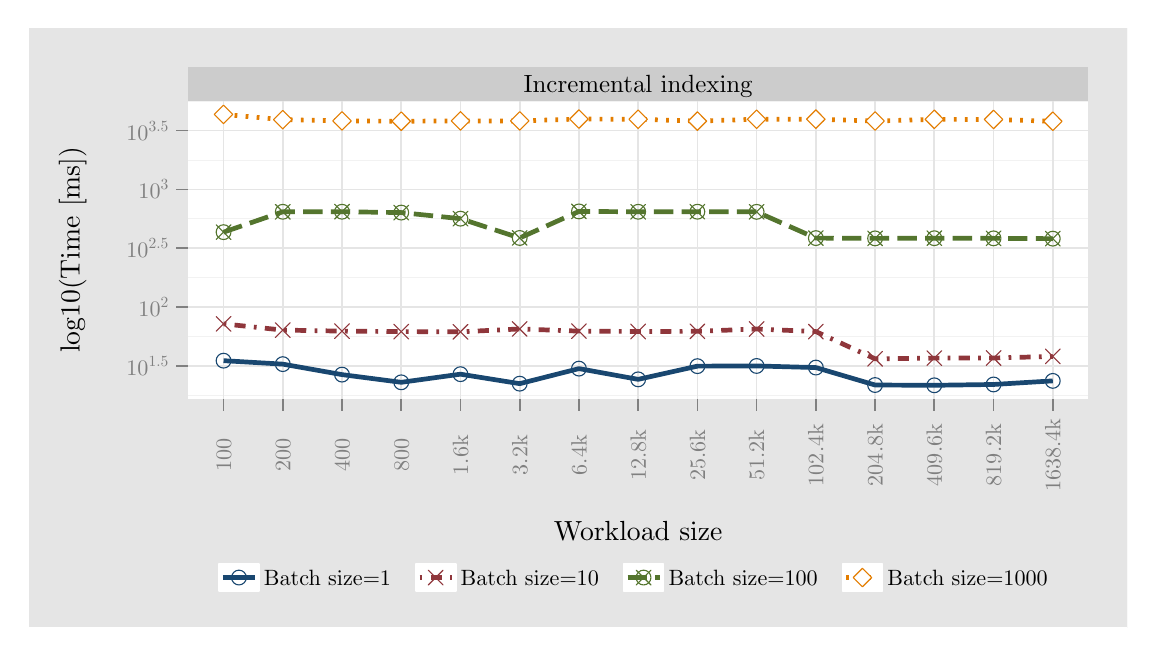
\begin{tikzpicture}[x=1pt,y=1pt]
\definecolor[named]{fillColor}{rgb}{1.00,1.00,1.00}
\path[use as bounding box,fill=fillColor,fill opacity=0.00] (0,0) rectangle (397.48,216.81);
\begin{scope}
\path[clip] (  0.00,  0.00) rectangle (397.48,216.81);
\definecolor[named]{drawColor}{rgb}{1.00,1.00,1.00}
\definecolor[named]{fillColor}{rgb}{0.90,0.90,0.90}

\path[draw=drawColor,line width= 0.6pt,line join=round,line cap=round,fill=fillColor] (  0.00,  0.00) rectangle (397.48,216.81);
\end{scope}
\begin{scope}
\path[clip] ( 57.94, 82.69) rectangle (383.26,190.36);
\definecolor[named]{fillColor}{rgb}{1.00,1.00,1.00}

\path[fill=fillColor] ( 57.94, 82.69) rectangle (383.26,190.36);
\definecolor[named]{drawColor}{rgb}{0.95,0.95,0.95}

\path[draw=drawColor,line width= 0.3pt,line join=round] ( 57.94, 84.04) --
	(383.26, 84.04);

\path[draw=drawColor,line width= 0.3pt,line join=round] ( 57.94,105.27) --
	(383.26,105.27);

\path[draw=drawColor,line width= 0.3pt,line join=round] ( 57.94,126.51) --
	(383.26,126.51);

\path[draw=drawColor,line width= 0.3pt,line join=round] ( 57.94,147.74) --
	(383.26,147.74);

\path[draw=drawColor,line width= 0.3pt,line join=round] ( 57.94,168.97) --
	(383.26,168.97);

\path[draw=drawColor,line width= 0.3pt,line join=round] ( 57.94,190.21) --
	(383.26,190.21);
\definecolor[named]{drawColor}{rgb}{0.90,0.90,0.90}

\path[draw=drawColor,line width= 0.6pt,line join=round] ( 57.94, 94.65) --
	(383.26, 94.65);

\path[draw=drawColor,line width= 0.6pt,line join=round] ( 57.94,115.89) --
	(383.26,115.89);

\path[draw=drawColor,line width= 0.6pt,line join=round] ( 57.94,137.12) --
	(383.26,137.12);

\path[draw=drawColor,line width= 0.6pt,line join=round] ( 57.94,158.36) --
	(383.26,158.36);

\path[draw=drawColor,line width= 0.6pt,line join=round] ( 57.94,179.59) --
	(383.26,179.59);

\path[draw=drawColor,line width= 0.6pt,line join=round] ( 70.78, 82.69) --
	( 70.78,190.36);

\path[draw=drawColor,line width= 0.6pt,line join=round] ( 92.18, 82.69) --
	( 92.18,190.36);

\path[draw=drawColor,line width= 0.6pt,line join=round] (113.58, 82.69) --
	(113.58,190.36);

\path[draw=drawColor,line width= 0.6pt,line join=round] (134.99, 82.69) --
	(134.99,190.36);

\path[draw=drawColor,line width= 0.6pt,line join=round] (156.39, 82.69) --
	(156.39,190.36);

\path[draw=drawColor,line width= 0.6pt,line join=round] (177.79, 82.69) --
	(177.79,190.36);

\path[draw=drawColor,line width= 0.6pt,line join=round] (199.20, 82.69) --
	(199.20,190.36);

\path[draw=drawColor,line width= 0.6pt,line join=round] (220.60, 82.69) --
	(220.60,190.36);

\path[draw=drawColor,line width= 0.6pt,line join=round] (242.00, 82.69) --
	(242.00,190.36);

\path[draw=drawColor,line width= 0.6pt,line join=round] (263.40, 82.69) --
	(263.40,190.36);

\path[draw=drawColor,line width= 0.6pt,line join=round] (284.81, 82.69) --
	(284.81,190.36);

\path[draw=drawColor,line width= 0.6pt,line join=round] (306.21, 82.69) --
	(306.21,190.36);

\path[draw=drawColor,line width= 0.6pt,line join=round] (327.61, 82.69) --
	(327.61,190.36);

\path[draw=drawColor,line width= 0.6pt,line join=round] (349.01, 82.69) --
	(349.01,190.36);

\path[draw=drawColor,line width= 0.6pt,line join=round] (370.42, 82.69) --
	(370.42,190.36);
\definecolor[named]{drawColor}{rgb}{0.10,0.28,0.44}

\path[draw=drawColor,line width= 1.7pt,line join=round] ( 70.78, 96.48) --
	( 92.18, 95.23) --
	(113.58, 91.44) --
	(134.99, 88.66) --
	(156.39, 91.60) --
	(177.79, 88.17) --
	(199.20, 93.61) --
	(220.60, 89.73) --
	(242.00, 94.50) --
	(263.40, 94.57) --
	(284.81, 93.99) --
	(306.21, 87.68) --
	(327.61, 87.58) --
	(349.01, 87.88) --
	(370.42, 89.18);
\definecolor[named]{drawColor}{rgb}{0.56,0.21,0.23}

\path[draw=drawColor,line width= 1.7pt,dash pattern=on 1pt off 3pt on 4pt off 3pt ,line join=round] ( 70.78,109.78) --
	( 92.18,107.53) --
	(113.58,107.16) --
	(134.99,106.99) --
	(156.39,106.91) --
	(177.79,107.94) --
	(199.20,107.16) --
	(220.60,107.03) --
	(242.00,107.08) --
	(263.40,107.93) --
	(284.81,106.99) --
	(306.21, 97.15) --
	(327.61, 97.40) --
	(349.01, 97.44) --
	(370.42, 98.02);
\definecolor[named]{drawColor}{rgb}{0.33,0.46,0.18}

\path[draw=drawColor,line width= 1.7pt,dash pattern=on 7pt off 3pt ,line join=round] ( 70.78,142.92) --
	( 92.18,150.28) --
	(113.58,150.30) --
	(134.99,149.99) --
	(156.39,147.79) --
	(177.79,140.82) --
	(199.20,150.41) --
	(220.60,150.28) --
	(242.00,150.30) --
	(263.40,150.26) --
	(284.81,140.77) --
	(306.21,140.67) --
	(327.61,140.73) --
	(349.01,140.68) --
	(370.42,140.57);
\definecolor[named]{drawColor}{rgb}{0.89,0.49,0.00}

\path[draw=drawColor,line width= 1.7pt,dash pattern=on 1pt off 3pt ,line join=round] ( 70.78,185.47) --
	( 92.18,183.57) --
	(113.58,183.10) --
	(134.99,183.00) --
	(156.39,183.12) --
	(177.79,183.12) --
	(199.20,183.79) --
	(220.60,183.71) --
	(242.00,183.04) --
	(263.40,183.73) --
	(284.81,183.75) --
	(306.21,183.07) --
	(327.61,183.68) --
	(349.01,183.64) --
	(370.42,182.99);
\definecolor[named]{drawColor}{rgb}{0.10,0.28,0.44}

\path[draw=drawColor,line width= 0.4pt,line join=round,line cap=round] ( 70.78, 96.48) circle (  2.67);
\definecolor[named]{drawColor}{rgb}{0.56,0.21,0.23}

\path[draw=drawColor,line width= 0.4pt,line join=round,line cap=round,fill=fillColor] ( 68.11,107.11) -- ( 73.45,112.45);

\path[draw=drawColor,line width= 0.4pt,line join=round,line cap=round,fill=fillColor] ( 68.11,112.45) -- ( 73.45,107.11);
\definecolor[named]{drawColor}{rgb}{0.33,0.46,0.18}

\path[draw=drawColor,line width= 0.4pt,line join=round,line cap=round] ( 70.78,142.92) circle (  2.67);

\path[draw=drawColor,line width= 0.4pt,line join=round,line cap=round] ( 68.11,140.25) -- ( 73.45,145.58);

\path[draw=drawColor,line width= 0.4pt,line join=round,line cap=round] ( 68.11,145.58) -- ( 73.45,140.25);
\definecolor[named]{drawColor}{rgb}{0.89,0.49,0.00}

\path[draw=drawColor,line width= 0.4pt,line join=round,line cap=round,fill=fillColor] ( 70.78,182.13) --
	( 74.12,185.47) --
	( 70.78,188.81) --
	( 67.44,185.47) --
	cycle;
\definecolor[named]{drawColor}{rgb}{0.10,0.28,0.44}

\path[draw=drawColor,line width= 0.4pt,line join=round,line cap=round] ( 92.18, 95.23) circle (  2.67);
\definecolor[named]{drawColor}{rgb}{0.56,0.21,0.23}

\path[draw=drawColor,line width= 0.4pt,line join=round,line cap=round,fill=fillColor] ( 89.51,104.86) -- ( 94.85,110.20);

\path[draw=drawColor,line width= 0.4pt,line join=round,line cap=round,fill=fillColor] ( 89.51,110.20) -- ( 94.85,104.86);
\definecolor[named]{drawColor}{rgb}{0.33,0.46,0.18}

\path[draw=drawColor,line width= 0.4pt,line join=round,line cap=round] ( 92.18,150.28) circle (  2.67);

\path[draw=drawColor,line width= 0.4pt,line join=round,line cap=round] ( 89.51,147.61) -- ( 94.85,152.95);

\path[draw=drawColor,line width= 0.4pt,line join=round,line cap=round] ( 89.51,152.95) -- ( 94.85,147.61);
\definecolor[named]{drawColor}{rgb}{0.89,0.49,0.00}

\path[draw=drawColor,line width= 0.4pt,line join=round,line cap=round,fill=fillColor] ( 92.18,180.23) --
	( 95.52,183.57) --
	( 92.18,186.91) --
	( 88.84,183.57) --
	cycle;
\definecolor[named]{drawColor}{rgb}{0.10,0.28,0.44}

\path[draw=drawColor,line width= 0.4pt,line join=round,line cap=round] (113.58, 91.44) circle (  2.67);
\definecolor[named]{drawColor}{rgb}{0.56,0.21,0.23}

\path[draw=drawColor,line width= 0.4pt,line join=round,line cap=round,fill=fillColor] (110.92,104.49) -- (116.25,109.83);

\path[draw=drawColor,line width= 0.4pt,line join=round,line cap=round,fill=fillColor] (110.92,109.83) -- (116.25,104.49);
\definecolor[named]{drawColor}{rgb}{0.33,0.46,0.18}

\path[draw=drawColor,line width= 0.4pt,line join=round,line cap=round] (113.58,150.30) circle (  2.67);

\path[draw=drawColor,line width= 0.4pt,line join=round,line cap=round] (110.92,147.64) -- (116.25,152.97);

\path[draw=drawColor,line width= 0.4pt,line join=round,line cap=round] (110.92,152.97) -- (116.25,147.64);
\definecolor[named]{drawColor}{rgb}{0.89,0.49,0.00}

\path[draw=drawColor,line width= 0.4pt,line join=round,line cap=round,fill=fillColor] (113.58,179.76) --
	(116.93,183.10) --
	(113.58,186.44) --
	(110.24,183.10) --
	cycle;
\definecolor[named]{drawColor}{rgb}{0.10,0.28,0.44}

\path[draw=drawColor,line width= 0.4pt,line join=round,line cap=round] (134.99, 88.66) circle (  2.67);
\definecolor[named]{drawColor}{rgb}{0.56,0.21,0.23}

\path[draw=drawColor,line width= 0.4pt,line join=round,line cap=round,fill=fillColor] (132.32,104.33) -- (137.65,109.66);

\path[draw=drawColor,line width= 0.4pt,line join=round,line cap=round,fill=fillColor] (132.32,109.66) -- (137.65,104.33);
\definecolor[named]{drawColor}{rgb}{0.33,0.46,0.18}

\path[draw=drawColor,line width= 0.4pt,line join=round,line cap=round] (134.99,149.99) circle (  2.67);

\path[draw=drawColor,line width= 0.4pt,line join=round,line cap=round] (132.32,147.32) -- (137.65,152.66);

\path[draw=drawColor,line width= 0.4pt,line join=round,line cap=round] (132.32,152.66) -- (137.65,147.32);
\definecolor[named]{drawColor}{rgb}{0.89,0.49,0.00}

\path[draw=drawColor,line width= 0.4pt,line join=round,line cap=round,fill=fillColor] (134.99,179.66) --
	(138.33,183.00) --
	(134.99,186.35) --
	(131.64,183.00) --
	cycle;
\definecolor[named]{drawColor}{rgb}{0.10,0.28,0.44}

\path[draw=drawColor,line width= 0.4pt,line join=round,line cap=round] (156.39, 91.60) circle (  2.67);
\definecolor[named]{drawColor}{rgb}{0.56,0.21,0.23}

\path[draw=drawColor,line width= 0.4pt,line join=round,line cap=round,fill=fillColor] (153.72,104.24) -- (159.06,109.58);

\path[draw=drawColor,line width= 0.4pt,line join=round,line cap=round,fill=fillColor] (153.72,109.58) -- (159.06,104.24);
\definecolor[named]{drawColor}{rgb}{0.33,0.46,0.18}

\path[draw=drawColor,line width= 0.4pt,line join=round,line cap=round] (156.39,147.79) circle (  2.67);

\path[draw=drawColor,line width= 0.4pt,line join=round,line cap=round] (153.72,145.13) -- (159.06,150.46);

\path[draw=drawColor,line width= 0.4pt,line join=round,line cap=round] (153.72,150.46) -- (159.06,145.13);
\definecolor[named]{drawColor}{rgb}{0.89,0.49,0.00}

\path[draw=drawColor,line width= 0.4pt,line join=round,line cap=round,fill=fillColor] (156.39,179.78) --
	(159.73,183.12) --
	(156.39,186.47) --
	(153.05,183.12) --
	cycle;
\definecolor[named]{drawColor}{rgb}{0.10,0.28,0.44}

\path[draw=drawColor,line width= 0.4pt,line join=round,line cap=round] (177.79, 88.17) circle (  2.67);
\definecolor[named]{drawColor}{rgb}{0.56,0.21,0.23}

\path[draw=drawColor,line width= 0.4pt,line join=round,line cap=round,fill=fillColor] (175.12,105.27) -- (180.46,110.60);

\path[draw=drawColor,line width= 0.4pt,line join=round,line cap=round,fill=fillColor] (175.12,110.60) -- (180.46,105.27);
\definecolor[named]{drawColor}{rgb}{0.33,0.46,0.18}

\path[draw=drawColor,line width= 0.4pt,line join=round,line cap=round] (177.79,140.82) circle (  2.67);

\path[draw=drawColor,line width= 0.4pt,line join=round,line cap=round] (175.12,138.15) -- (180.46,143.49);

\path[draw=drawColor,line width= 0.4pt,line join=round,line cap=round] (175.12,143.49) -- (180.46,138.15);
\definecolor[named]{drawColor}{rgb}{0.89,0.49,0.00}

\path[draw=drawColor,line width= 0.4pt,line join=round,line cap=round,fill=fillColor] (177.79,179.78) --
	(181.14,183.12) --
	(177.79,186.46) --
	(174.45,183.12) --
	cycle;
\definecolor[named]{drawColor}{rgb}{0.10,0.28,0.44}

\path[draw=drawColor,line width= 0.4pt,line join=round,line cap=round] (199.20, 93.61) circle (  2.67);
\definecolor[named]{drawColor}{rgb}{0.56,0.21,0.23}

\path[draw=drawColor,line width= 0.4pt,line join=round,line cap=round,fill=fillColor] (196.53,104.49) -- (201.86,109.83);

\path[draw=drawColor,line width= 0.4pt,line join=round,line cap=round,fill=fillColor] (196.53,109.83) -- (201.86,104.49);
\definecolor[named]{drawColor}{rgb}{0.33,0.46,0.18}

\path[draw=drawColor,line width= 0.4pt,line join=round,line cap=round] (199.20,150.41) circle (  2.67);

\path[draw=drawColor,line width= 0.4pt,line join=round,line cap=round] (196.53,147.75) -- (201.86,153.08);

\path[draw=drawColor,line width= 0.4pt,line join=round,line cap=round] (196.53,153.08) -- (201.86,147.75);
\definecolor[named]{drawColor}{rgb}{0.89,0.49,0.00}

\path[draw=drawColor,line width= 0.4pt,line join=round,line cap=round,fill=fillColor] (199.20,180.44) --
	(202.54,183.79) --
	(199.20,187.13) --
	(195.85,183.79) --
	cycle;
\definecolor[named]{drawColor}{rgb}{0.10,0.28,0.44}

\path[draw=drawColor,line width= 0.4pt,line join=round,line cap=round] (220.60, 89.73) circle (  2.67);
\definecolor[named]{drawColor}{rgb}{0.56,0.21,0.23}

\path[draw=drawColor,line width= 0.4pt,line join=round,line cap=round,fill=fillColor] (217.93,104.36) -- (223.27,109.70);

\path[draw=drawColor,line width= 0.4pt,line join=round,line cap=round,fill=fillColor] (217.93,109.70) -- (223.27,104.36);
\definecolor[named]{drawColor}{rgb}{0.33,0.46,0.18}

\path[draw=drawColor,line width= 0.4pt,line join=round,line cap=round] (220.60,150.28) circle (  2.67);

\path[draw=drawColor,line width= 0.4pt,line join=round,line cap=round] (217.93,147.62) -- (223.27,152.95);

\path[draw=drawColor,line width= 0.4pt,line join=round,line cap=round] (217.93,152.95) -- (223.27,147.62);
\definecolor[named]{drawColor}{rgb}{0.89,0.49,0.00}

\path[draw=drawColor,line width= 0.4pt,line join=round,line cap=round,fill=fillColor] (220.60,180.36) --
	(223.94,183.71) --
	(220.60,187.05) --
	(217.25,183.71) --
	cycle;
\definecolor[named]{drawColor}{rgb}{0.10,0.28,0.44}

\path[draw=drawColor,line width= 0.4pt,line join=round,line cap=round] (242.00, 94.50) circle (  2.67);
\definecolor[named]{drawColor}{rgb}{0.56,0.21,0.23}

\path[draw=drawColor,line width= 0.4pt,line join=round,line cap=round,fill=fillColor] (239.33,104.41) -- (244.67,109.75);

\path[draw=drawColor,line width= 0.4pt,line join=round,line cap=round,fill=fillColor] (239.33,109.75) -- (244.67,104.41);
\definecolor[named]{drawColor}{rgb}{0.33,0.46,0.18}

\path[draw=drawColor,line width= 0.4pt,line join=round,line cap=round] (242.00,150.30) circle (  2.67);

\path[draw=drawColor,line width= 0.4pt,line join=round,line cap=round] (239.33,147.64) -- (244.67,152.97);

\path[draw=drawColor,line width= 0.4pt,line join=round,line cap=round] (239.33,152.97) -- (244.67,147.64);
\definecolor[named]{drawColor}{rgb}{0.89,0.49,0.00}

\path[draw=drawColor,line width= 0.4pt,line join=round,line cap=round,fill=fillColor] (242.00,179.70) --
	(245.34,183.04) --
	(242.00,186.39) --
	(238.66,183.04) --
	cycle;
\definecolor[named]{drawColor}{rgb}{0.10,0.28,0.44}

\path[draw=drawColor,line width= 0.4pt,line join=round,line cap=round] (263.40, 94.57) circle (  2.67);
\definecolor[named]{drawColor}{rgb}{0.56,0.21,0.23}

\path[draw=drawColor,line width= 0.4pt,line join=round,line cap=round,fill=fillColor] (260.74,105.26) -- (266.07,110.60);

\path[draw=drawColor,line width= 0.4pt,line join=round,line cap=round,fill=fillColor] (260.74,110.60) -- (266.07,105.26);
\definecolor[named]{drawColor}{rgb}{0.33,0.46,0.18}

\path[draw=drawColor,line width= 0.4pt,line join=round,line cap=round] (263.40,150.26) circle (  2.67);

\path[draw=drawColor,line width= 0.4pt,line join=round,line cap=round] (260.74,147.60) -- (266.07,152.93);

\path[draw=drawColor,line width= 0.4pt,line join=round,line cap=round] (260.74,152.93) -- (266.07,147.60);
\definecolor[named]{drawColor}{rgb}{0.89,0.49,0.00}

\path[draw=drawColor,line width= 0.4pt,line join=round,line cap=round,fill=fillColor] (263.40,180.39) --
	(266.75,183.73) --
	(263.40,187.08) --
	(260.06,183.73) --
	cycle;
\definecolor[named]{drawColor}{rgb}{0.10,0.28,0.44}

\path[draw=drawColor,line width= 0.4pt,line join=round,line cap=round] (284.81, 93.99) circle (  2.67);
\definecolor[named]{drawColor}{rgb}{0.56,0.21,0.23}

\path[draw=drawColor,line width= 0.4pt,line join=round,line cap=round,fill=fillColor] (282.14,104.32) -- (287.47,109.65);

\path[draw=drawColor,line width= 0.4pt,line join=round,line cap=round,fill=fillColor] (282.14,109.65) -- (287.47,104.32);
\definecolor[named]{drawColor}{rgb}{0.33,0.46,0.18}

\path[draw=drawColor,line width= 0.4pt,line join=round,line cap=round] (284.81,140.77) circle (  2.67);

\path[draw=drawColor,line width= 0.4pt,line join=round,line cap=round] (282.14,138.11) -- (287.47,143.44);

\path[draw=drawColor,line width= 0.4pt,line join=round,line cap=round] (282.14,143.44) -- (287.47,138.11);
\definecolor[named]{drawColor}{rgb}{0.89,0.49,0.00}

\path[draw=drawColor,line width= 0.4pt,line join=round,line cap=round,fill=fillColor] (284.81,180.41) --
	(288.15,183.75) --
	(284.81,187.10) --
	(281.46,183.75) --
	cycle;
\definecolor[named]{drawColor}{rgb}{0.10,0.28,0.44}

\path[draw=drawColor,line width= 0.4pt,line join=round,line cap=round] (306.21, 87.68) circle (  2.67);
\definecolor[named]{drawColor}{rgb}{0.56,0.21,0.23}

\path[draw=drawColor,line width= 0.4pt,line join=round,line cap=round,fill=fillColor] (303.54, 94.48) -- (308.88, 99.81);

\path[draw=drawColor,line width= 0.4pt,line join=round,line cap=round,fill=fillColor] (303.54, 99.81) -- (308.88, 94.48);
\definecolor[named]{drawColor}{rgb}{0.33,0.46,0.18}

\path[draw=drawColor,line width= 0.4pt,line join=round,line cap=round] (306.21,140.67) circle (  2.67);

\path[draw=drawColor,line width= 0.4pt,line join=round,line cap=round] (303.54,138.01) -- (308.88,143.34);

\path[draw=drawColor,line width= 0.4pt,line join=round,line cap=round] (303.54,143.34) -- (308.88,138.01);
\definecolor[named]{drawColor}{rgb}{0.89,0.49,0.00}

\path[draw=drawColor,line width= 0.4pt,line join=round,line cap=round,fill=fillColor] (306.21,179.73) --
	(309.55,183.07) --
	(306.21,186.42) --
	(302.87,183.07) --
	cycle;
\definecolor[named]{drawColor}{rgb}{0.10,0.28,0.44}

\path[draw=drawColor,line width= 0.4pt,line join=round,line cap=round] (327.61, 87.58) circle (  2.67);
\definecolor[named]{drawColor}{rgb}{0.56,0.21,0.23}

\path[draw=drawColor,line width= 0.4pt,line join=round,line cap=round,fill=fillColor] (324.94, 94.73) -- (330.28,100.07);

\path[draw=drawColor,line width= 0.4pt,line join=round,line cap=round,fill=fillColor] (324.94,100.07) -- (330.28, 94.73);
\definecolor[named]{drawColor}{rgb}{0.33,0.46,0.18}

\path[draw=drawColor,line width= 0.4pt,line join=round,line cap=round] (327.61,140.73) circle (  2.67);

\path[draw=drawColor,line width= 0.4pt,line join=round,line cap=round] (324.94,138.07) -- (330.28,143.40);

\path[draw=drawColor,line width= 0.4pt,line join=round,line cap=round] (324.94,143.40) -- (330.28,138.07);
\definecolor[named]{drawColor}{rgb}{0.89,0.49,0.00}

\path[draw=drawColor,line width= 0.4pt,line join=round,line cap=round,fill=fillColor] (327.61,180.34) --
	(330.95,183.68) --
	(327.61,187.03) --
	(324.27,183.68) --
	cycle;
\definecolor[named]{drawColor}{rgb}{0.10,0.28,0.44}

\path[draw=drawColor,line width= 0.4pt,line join=round,line cap=round] (349.01, 87.88) circle (  2.67);
\definecolor[named]{drawColor}{rgb}{0.56,0.21,0.23}

\path[draw=drawColor,line width= 0.4pt,line join=round,line cap=round,fill=fillColor] (346.35, 94.77) -- (351.68,100.11);

\path[draw=drawColor,line width= 0.4pt,line join=round,line cap=round,fill=fillColor] (346.35,100.11) -- (351.68, 94.77);
\definecolor[named]{drawColor}{rgb}{0.33,0.46,0.18}

\path[draw=drawColor,line width= 0.4pt,line join=round,line cap=round] (349.01,140.68) circle (  2.67);

\path[draw=drawColor,line width= 0.4pt,line join=round,line cap=round] (346.35,138.02) -- (351.68,143.35);

\path[draw=drawColor,line width= 0.4pt,line join=round,line cap=round] (346.35,143.35) -- (351.68,138.02);
\definecolor[named]{drawColor}{rgb}{0.89,0.49,0.00}

\path[draw=drawColor,line width= 0.4pt,line join=round,line cap=round,fill=fillColor] (349.01,180.29) --
	(352.36,183.64) --
	(349.01,186.98) --
	(345.67,183.64) --
	cycle;
\definecolor[named]{drawColor}{rgb}{0.10,0.28,0.44}

\path[draw=drawColor,line width= 0.4pt,line join=round,line cap=round] (370.42, 89.18) circle (  2.67);
\definecolor[named]{drawColor}{rgb}{0.56,0.21,0.23}

\path[draw=drawColor,line width= 0.4pt,line join=round,line cap=round,fill=fillColor] (367.75, 95.35) -- (373.08,100.69);

\path[draw=drawColor,line width= 0.4pt,line join=round,line cap=round,fill=fillColor] (367.75,100.69) -- (373.08, 95.35);
\definecolor[named]{drawColor}{rgb}{0.33,0.46,0.18}

\path[draw=drawColor,line width= 0.4pt,line join=round,line cap=round] (370.42,140.57) circle (  2.67);

\path[draw=drawColor,line width= 0.4pt,line join=round,line cap=round] (367.75,137.90) -- (373.08,143.23);

\path[draw=drawColor,line width= 0.4pt,line join=round,line cap=round] (367.75,143.23) -- (373.08,137.90);
\definecolor[named]{drawColor}{rgb}{0.89,0.49,0.00}

\path[draw=drawColor,line width= 0.4pt,line join=round,line cap=round,fill=fillColor] (370.42,179.65) --
	(373.76,182.99) --
	(370.42,186.34) --
	(367.07,182.99) --
	cycle;
\end{scope}
\begin{scope}
\path[clip] (  0.00,  0.00) rectangle (397.48,216.81);
\definecolor[named]{fillColor}{rgb}{0.80,0.80,0.80}

\path[fill=fillColor] ( 57.94,190.36) rectangle (383.26,202.58);
\definecolor[named]{drawColor}{rgb}{0.00,0.00,0.00}

\node[text=drawColor,anchor=base,inner sep=0pt, outer sep=0pt, scale=  0.90] at (220.60,193.37) {Incremental indexing};
\end{scope}
\begin{scope}
\path[clip] (  0.00,  0.00) rectangle (397.48,216.81);
\definecolor[named]{drawColor}{rgb}{0.50,0.50,0.50}

\node[text=drawColor,anchor=base west,inner sep=0pt, outer sep=0pt, scale=  0.80] at ( 35.67, 91.22) {10};

\node[text=drawColor,anchor=base west,inner sep=0pt, outer sep=0pt, scale=  0.56] at ( 43.67, 94.49) {1};

\node[text=drawColor,anchor=base west,inner sep=0pt, outer sep=0pt, scale=  0.56] at ( 46.47, 94.49) {.};

\node[text=drawColor,anchor=base west,inner sep=0pt, outer sep=0pt, scale=  0.56] at ( 48.02, 94.49) {5};

\node[text=drawColor,anchor=base west,inner sep=0pt, outer sep=0pt, scale=  0.80] at ( 40.03,112.46) {10};

\node[text=drawColor,anchor=base west,inner sep=0pt, outer sep=0pt, scale=  0.56] at ( 48.02,115.73) {2};

\node[text=drawColor,anchor=base west,inner sep=0pt, outer sep=0pt, scale=  0.80] at ( 35.67,133.69) {10};

\node[text=drawColor,anchor=base west,inner sep=0pt, outer sep=0pt, scale=  0.56] at ( 43.67,136.96) {2};

\node[text=drawColor,anchor=base west,inner sep=0pt, outer sep=0pt, scale=  0.56] at ( 46.47,136.96) {.};

\node[text=drawColor,anchor=base west,inner sep=0pt, outer sep=0pt, scale=  0.56] at ( 48.02,136.96) {5};

\node[text=drawColor,anchor=base west,inner sep=0pt, outer sep=0pt, scale=  0.80] at ( 40.03,154.93) {10};

\node[text=drawColor,anchor=base west,inner sep=0pt, outer sep=0pt, scale=  0.56] at ( 48.02,158.20) {3};

\node[text=drawColor,anchor=base west,inner sep=0pt, outer sep=0pt, scale=  0.80] at ( 35.67,176.16) {10};

\node[text=drawColor,anchor=base west,inner sep=0pt, outer sep=0pt, scale=  0.56] at ( 43.67,179.43) {3};

\node[text=drawColor,anchor=base west,inner sep=0pt, outer sep=0pt, scale=  0.56] at ( 46.47,179.43) {.};

\node[text=drawColor,anchor=base west,inner sep=0pt, outer sep=0pt, scale=  0.56] at ( 48.02,179.43) {5};
\end{scope}
\begin{scope}
\path[clip] (  0.00,  0.00) rectangle (397.48,216.81);
\definecolor[named]{drawColor}{rgb}{0.50,0.50,0.50}

\path[draw=drawColor,line width= 0.6pt,line join=round] ( 53.67, 94.65) --
	( 57.94, 94.65);

\path[draw=drawColor,line width= 0.6pt,line join=round] ( 53.67,115.89) --
	( 57.94,115.89);

\path[draw=drawColor,line width= 0.6pt,line join=round] ( 53.67,137.12) --
	( 57.94,137.12);

\path[draw=drawColor,line width= 0.6pt,line join=round] ( 53.67,158.36) --
	( 57.94,158.36);

\path[draw=drawColor,line width= 0.6pt,line join=round] ( 53.67,179.59) --
	( 57.94,179.59);
\end{scope}
\begin{scope}
\path[clip] (  0.00,  0.00) rectangle (397.48,216.81);
\definecolor[named]{drawColor}{rgb}{0.50,0.50,0.50}

\path[draw=drawColor,line width= 0.6pt,line join=round] ( 70.78, 78.42) --
	( 70.78, 82.69);

\path[draw=drawColor,line width= 0.6pt,line join=round] ( 92.18, 78.42) --
	( 92.18, 82.69);

\path[draw=drawColor,line width= 0.6pt,line join=round] (113.58, 78.42) --
	(113.58, 82.69);

\path[draw=drawColor,line width= 0.6pt,line join=round] (134.99, 78.42) --
	(134.99, 82.69);

\path[draw=drawColor,line width= 0.6pt,line join=round] (156.39, 78.42) --
	(156.39, 82.69);

\path[draw=drawColor,line width= 0.6pt,line join=round] (177.79, 78.42) --
	(177.79, 82.69);

\path[draw=drawColor,line width= 0.6pt,line join=round] (199.20, 78.42) --
	(199.20, 82.69);

\path[draw=drawColor,line width= 0.6pt,line join=round] (220.60, 78.42) --
	(220.60, 82.69);

\path[draw=drawColor,line width= 0.6pt,line join=round] (242.00, 78.42) --
	(242.00, 82.69);

\path[draw=drawColor,line width= 0.6pt,line join=round] (263.40, 78.42) --
	(263.40, 82.69);

\path[draw=drawColor,line width= 0.6pt,line join=round] (284.81, 78.42) --
	(284.81, 82.69);

\path[draw=drawColor,line width= 0.6pt,line join=round] (306.21, 78.42) --
	(306.21, 82.69);

\path[draw=drawColor,line width= 0.6pt,line join=round] (327.61, 78.42) --
	(327.61, 82.69);

\path[draw=drawColor,line width= 0.6pt,line join=round] (349.01, 78.42) --
	(349.01, 82.69);

\path[draw=drawColor,line width= 0.6pt,line join=round] (370.42, 78.42) --
	(370.42, 82.69);
\end{scope}
\begin{scope}
\path[clip] (  0.00,  0.00) rectangle (397.48,216.81);
\definecolor[named]{drawColor}{rgb}{0.50,0.50,0.50}

\node[text=drawColor,rotate= 90.00,anchor=base,inner sep=0pt, outer sep=0pt, scale=  0.80] at ( 73.53, 62.36) {100};

\node[text=drawColor,rotate= 90.00,anchor=base,inner sep=0pt, outer sep=0pt, scale=  0.80] at ( 94.94, 62.36) {200};

\node[text=drawColor,rotate= 90.00,anchor=base,inner sep=0pt, outer sep=0pt, scale=  0.80] at (116.34, 62.36) {400};

\node[text=drawColor,rotate= 90.00,anchor=base,inner sep=0pt, outer sep=0pt, scale=  0.80] at (137.74, 62.36) {800};

\node[text=drawColor,rotate= 90.00,anchor=base,inner sep=0pt, outer sep=0pt, scale=  0.80] at (159.14, 62.36) {1.6k};

\node[text=drawColor,rotate= 90.00,anchor=base,inner sep=0pt, outer sep=0pt, scale=  0.80] at (180.55, 62.36) {3.2k};

\node[text=drawColor,rotate= 90.00,anchor=base,inner sep=0pt, outer sep=0pt, scale=  0.80] at (201.95, 62.36) {6.4k};

\node[text=drawColor,rotate= 90.00,anchor=base,inner sep=0pt, outer sep=0pt, scale=  0.80] at (223.35, 62.36) {12.8k};

\node[text=drawColor,rotate= 90.00,anchor=base,inner sep=0pt, outer sep=0pt, scale=  0.80] at (244.76, 62.36) {25.6k};

\node[text=drawColor,rotate= 90.00,anchor=base,inner sep=0pt, outer sep=0pt, scale=  0.80] at (266.16, 62.36) {51.2k};

\node[text=drawColor,rotate= 90.00,anchor=base,inner sep=0pt, outer sep=0pt, scale=  0.80] at (287.56, 62.36) {102.4k};

\node[text=drawColor,rotate= 90.00,anchor=base,inner sep=0pt, outer sep=0pt, scale=  0.80] at (308.96, 62.36) {204.8k};

\node[text=drawColor,rotate= 90.00,anchor=base,inner sep=0pt, outer sep=0pt, scale=  0.80] at (330.37, 62.36) {409.6k};

\node[text=drawColor,rotate= 90.00,anchor=base,inner sep=0pt, outer sep=0pt, scale=  0.80] at (351.77, 62.36) {819.2k};

\node[text=drawColor,rotate= 90.00,anchor=base,inner sep=0pt, outer sep=0pt, scale=  0.80] at (373.17, 62.36) {1638.4k};
\end{scope}
\begin{scope}
\path[clip] (  0.00,  0.00) rectangle (397.48,216.81);
\definecolor[named]{drawColor}{rgb}{0.00,0.00,0.00}

\node[text=drawColor,anchor=base,inner sep=0pt, outer sep=0pt, scale=  1.00] at (220.60, 31.41) {Workload size};
\end{scope}
\begin{scope}
\path[clip] (  0.00,  0.00) rectangle (397.48,216.81);
\definecolor[named]{drawColor}{rgb}{0.00,0.00,0.00}

\node[text=drawColor,rotate= 90.00,anchor=base,inner sep=0pt, outer sep=0pt, scale=  1.00] at ( 18.80,136.53) {log10(Time [ms])};
\end{scope}
\begin{scope}
\path[clip] (  0.00,  0.00) rectangle (397.48,216.81);
\definecolor[named]{fillColor}{rgb}{0.90,0.90,0.90}

\path[fill=fillColor] ( 61.23,  8.87) rectangle (379.97, 27.36);
\end{scope}
\begin{scope}
\path[clip] (  0.00,  0.00) rectangle (397.48,216.81);
\definecolor[named]{drawColor}{rgb}{1.00,1.00,1.00}
\definecolor[named]{fillColor}{rgb}{1.00,1.00,1.00}

\path[draw=drawColor,line width= 0.6pt,line join=round,line cap=round,fill=fillColor] ( 69.11, 13.14) rectangle ( 83.56, 23.09);
\end{scope}
\begin{scope}
\path[clip] (  0.00,  0.00) rectangle (397.48,216.81);
\definecolor[named]{drawColor}{rgb}{0.10,0.28,0.44}

\path[draw=drawColor,line width= 1.7pt,line join=round] ( 70.56, 18.11) -- ( 82.12, 18.11);
\end{scope}
\begin{scope}
\path[clip] (  0.00,  0.00) rectangle (397.48,216.81);
\definecolor[named]{drawColor}{rgb}{0.10,0.28,0.44}

\path[draw=drawColor,line width= 0.4pt,line join=round,line cap=round] ( 76.34, 18.11) circle (  2.67);
\end{scope}
\begin{scope}
\path[clip] (  0.00,  0.00) rectangle (397.48,216.81);
\definecolor[named]{drawColor}{rgb}{1.00,1.00,1.00}
\definecolor[named]{fillColor}{rgb}{1.00,1.00,1.00}

\path[draw=drawColor,line width= 0.6pt,line join=round,line cap=round,fill=fillColor] (140.21, 13.14) rectangle (154.66, 23.09);
\end{scope}
\begin{scope}
\path[clip] (  0.00,  0.00) rectangle (397.48,216.81);
\definecolor[named]{drawColor}{rgb}{0.56,0.21,0.23}

\path[draw=drawColor,line width= 1.7pt,dash pattern=on 1pt off 3pt on 4pt off 3pt ,line join=round] (141.66, 18.11) -- (153.22, 18.11);
\end{scope}
\begin{scope}
\path[clip] (  0.00,  0.00) rectangle (397.48,216.81);
\definecolor[named]{drawColor}{rgb}{0.56,0.21,0.23}
\definecolor[named]{fillColor}{rgb}{1.00,1.00,1.00}

\path[draw=drawColor,line width= 0.4pt,line join=round,line cap=round,fill=fillColor] (144.77, 15.45) -- (150.11, 20.78);

\path[draw=drawColor,line width= 0.4pt,line join=round,line cap=round,fill=fillColor] (144.77, 20.78) -- (150.11, 15.45);
\end{scope}
\begin{scope}
\path[clip] (  0.00,  0.00) rectangle (397.48,216.81);
\definecolor[named]{drawColor}{rgb}{1.00,1.00,1.00}
\definecolor[named]{fillColor}{rgb}{1.00,1.00,1.00}

\path[draw=drawColor,line width= 0.6pt,line join=round,line cap=round,fill=fillColor] (215.31, 13.14) rectangle (229.76, 23.09);
\end{scope}
\begin{scope}
\path[clip] (  0.00,  0.00) rectangle (397.48,216.81);
\definecolor[named]{drawColor}{rgb}{0.33,0.46,0.18}

\path[draw=drawColor,line width= 1.7pt,dash pattern=on 7pt off 3pt ,line join=round] (216.76, 18.11) -- (228.32, 18.11);
\end{scope}
\begin{scope}
\path[clip] (  0.00,  0.00) rectangle (397.48,216.81);
\definecolor[named]{drawColor}{rgb}{0.33,0.46,0.18}

\path[draw=drawColor,line width= 0.4pt,line join=round,line cap=round] (222.54, 18.11) circle (  2.67);

\path[draw=drawColor,line width= 0.4pt,line join=round,line cap=round] (219.87, 15.45) -- (225.20, 20.78);

\path[draw=drawColor,line width= 0.4pt,line join=round,line cap=round] (219.87, 20.78) -- (225.20, 15.45);
\end{scope}
\begin{scope}
\path[clip] (  0.00,  0.00) rectangle (397.48,216.81);
\definecolor[named]{drawColor}{rgb}{1.00,1.00,1.00}
\definecolor[named]{fillColor}{rgb}{1.00,1.00,1.00}

\path[draw=drawColor,line width= 0.6pt,line join=round,line cap=round,fill=fillColor] (294.41, 13.14) rectangle (308.86, 23.09);
\end{scope}
\begin{scope}
\path[clip] (  0.00,  0.00) rectangle (397.48,216.81);
\definecolor[named]{drawColor}{rgb}{0.89,0.49,0.00}

\path[draw=drawColor,line width= 1.7pt,dash pattern=on 1pt off 3pt ,line join=round] (295.85, 18.11) -- (307.42, 18.11);
\end{scope}
\begin{scope}
\path[clip] (  0.00,  0.00) rectangle (397.48,216.81);
\definecolor[named]{drawColor}{rgb}{0.89,0.49,0.00}
\definecolor[named]{fillColor}{rgb}{1.00,1.00,1.00}

\path[draw=drawColor,line width= 0.4pt,line join=round,line cap=round,fill=fillColor] (301.64, 14.77) --
	(304.98, 18.11) --
	(301.64, 21.46) --
	(298.29, 18.11) --
	cycle;
\end{scope}
\begin{scope}
\path[clip] (  0.00,  0.00) rectangle (397.48,216.81);
\definecolor[named]{drawColor}{rgb}{0.00,0.00,0.00}

\node[text=drawColor,anchor=base west,inner sep=0pt, outer sep=0pt, scale=  0.80] at ( 85.37, 15.36) {Batch size=1 $\;\;$};
\end{scope}
\begin{scope}
\path[clip] (  0.00,  0.00) rectangle (397.48,216.81);
\definecolor[named]{drawColor}{rgb}{0.00,0.00,0.00}

\node[text=drawColor,anchor=base west,inner sep=0pt, outer sep=0pt, scale=  0.80] at (156.47, 15.36) {Batch size=10 $\;\;$};
\end{scope}
\begin{scope}
\path[clip] (  0.00,  0.00) rectangle (397.48,216.81);
\definecolor[named]{drawColor}{rgb}{0.00,0.00,0.00}

\node[text=drawColor,anchor=base west,inner sep=0pt, outer sep=0pt, scale=  0.80] at (231.57, 15.36) {Batch size=100 $\;\;$};
\end{scope}
\begin{scope}
\path[clip] (  0.00,  0.00) rectangle (397.48,216.81);
\definecolor[named]{drawColor}{rgb}{0.00,0.00,0.00}

\node[text=drawColor,anchor=base west,inner sep=0pt, outer sep=0pt, scale=  0.80] at (310.67, 15.36) {Batch size=1000 $\;\;$};
\end{scope}
\end{tikzpicture}

 }
 \caption[Impact of batch size on indexing\index{Index} performance]{Incremental Index documents update operations performance benchmarks.}
 \label{fig:experimentation:performance:indexing:incremental-indexing}
\end{figure}

\subparagraph{Discussion}

The conversion process of records to Apache Solr ingest format takes up a considerable amount of time during parsing. In addition, it is significantly faster to schedule commits for large sets of newer records in contrast to issuing commits after addition of each record, since the cumulative commit times for individual items in a typical batch are avoided.

%%\subsubsection{Discussion}
%%\label{sec:evaluation:performance:indexing:discussion}

%%\subsubsection{Conclusion}
%%\label{sec:evaluation:performance:indexing:conclusion}

%%xxx

\subsubsection[OAI-PMH]{OAI-PMH data provider}\index{OAI-PMH!Data Provider}
\label{sec:evaluation:performance:oaipmh-data-provider}

The main objective of experiments associated with this aspect was to determine
the performance of an integrated file-based collection OAI-PMH data provider\index{OAI-PMH!Data Provider} in
relation to the collection size.

The XMLFile\index{XMLFile} Perl\index{Perl} data provider\index{OAI-PMH!Data Provider} module \citep{Suleman2002} was used to conduct the
experiments. The module was configured and deployed within a
mod\_perl\footnote{An Apache/2.x HTTP server embedded Perl interpreter}
enabled Apache 2.2.22 Web server\index{Apache!Apache/2.x}. The following factors were considered,
relative to the workloads described in Section~\ref{sec:evaluation:performance:test-environment:workload-design}.

\begin{itemize}
 \item The collection structure
 \item The size of the resumptionToken
\end{itemize}

\paragraph{Experiment: OAI-PMH data provider\index{OAI-PMH!Data Provider} baseline benchmarks}
\label{sec:evaluation:performance:oaipmh-data-provider:experiment1}

This experiment was conducted to derive baseline results for a basic OAI-PMH
data provider\index{OAI-PMH!Data Provider} environment set up.

\subparagraph{Methodology} %\hspace*{\fill} \\ % provision for dirtree

%\bigskip
The OAI-PMH data provider\index{OAI-PMH!Data Provider} for each archive was configured with a resumptionToken of
1000 and the records in each workload\index{Workload} arranged in a one-level hierarchical
structure, as shown in Figure~\ref{fig:experimentation:performance:workload-design:directory-structures:dataset1}

The tests performed involved submitting GetRecord\index{OAI-PMH!Verbs!GetRecord}, ListIdentifiers\index{OAI-PMH!Verbs!ListIdentifiers}, ListRecords\index{OAI-PMH!Verbs!ListRecords}, and ListSets\index{OAI-PMH!Verbs!ListSets} requests to each of the individual 15 workloads.\index{Workload} Siege\index{Siege} was used to to simulate a single user request with a total of 5 repeated runs for each request; the average response times for each case were then recorded.

\subparagraph{Results}

The response times for the four OAI-PMH verbs\index{OAI-PMH!Verbs} are shown in Figure~\ref{fig:experimentation:performance:oaipmh:verbs-baseline}.

% 
% 
\begin{comment}workloads.\index{Workload}
\tablespacing
%\begin{longtable}{p{0.10\linewidth} p{0.15\linewidth}
%p{0.20\linewidth} p{0.15\linewidth} p{0.15\linewidth}}
%%%%%\begin{longtable}{ccccc}
\begin{longtable}{
>{\arraybackslash}m{0.07\linewidth}|
>{\centering\arraybackslash}m{0.15\linewidth}|
>{\centering\arraybackslash}m{0.20\linewidth}|
>{\centering\arraybackslash}m{0.15\linewidth}|
>{\centering\arraybackslash}m{0.12\linewidth}
}

\caption{Response times for OAI-PMH verb requests}
\label{tab:experimentation:performance:oaipmh:verbs-baseline} \\

 %%%%%\toprule
 \hline
 %%{} &
 %%\multicolumn{4}{c}{\textbf{OAI-PMH Verb}}\\
 %%\midrule
 {} &
 \textbf{GetRecord} &
 \textbf{ListIdentifiers} &
 \textbf{ListRecords} &
 \textbf{ListSets} \\
 %%%%%\midrule
 \hline \hline
 \endfirsthead

 \caption[]{(continued)}\\
 %%%%%\toprule
 \hline
 %%{} &
 %%\multicolumn{4}{c}{\textbf{OAI-PMH Verb}}\\
 %%\midrule
 {} &
 \textbf{GetRecord} &
 \textbf{ListIdentifiers} &
 \textbf{ListRecords} &
 \textbf{ListSets} \\
 %%%%%%\midrule
 \hline \hline
 \endhead

 % Page footer
 %%%%%\midrule
 \hline
 \multicolumn{5}{r}{(Continued on next page)} \\
 \endfoot

 % Last page footer
 \bottomrule
 \endlastfoot

 \textbf{W1} & {\tablenum[table-format=6]{10}} & {\tablenum[table-format=6]{10}} & {\tablenum[table-format=6]{480}} & {\tablenum[table-format=6]{0}} \\ 
 \textbf{W2} & {\tablenum[table-format=6]{10}} & {\tablenum[table-format=6]{20}} & {\tablenum[table-format=6]{980}} & {\tablenum[table-format=6]{10}} \\ 
 \textbf{W3} & {\tablenum[table-format=6]{10}} & {\tablenum[table-format=6]{60}} & {\tablenum[table-format=6]{2000}} & {\tablenum[table-format=6]{0}} \\ 
 \textbf{W4} & {\tablenum[table-format=6]{20}} & {\tablenum[table-format=6]{170}} & {\tablenum[table-format=6]{4120}} & {\tablenum[table-format=6]{10}} \\ 
 \textbf{W5} & {\tablenum[table-format=6]{20}} & {\tablenum[table-format=6]{390}} & {\tablenum[table-format=6]{5410}} & {\tablenum[table-format=6]{10}} \\ 
 \textbf{W6} & {\tablenum[table-format=6]{50}} & {\tablenum[table-format=6]{770}} & {\tablenum[table-format=6]{5940}} & {\tablenum[table-format=6]{20}} \\ 
 \textbf{W7} & {\tablenum[table-format=6]{80}} & {\tablenum[table-format=6]{1530}} & {\tablenum[table-format=6]{6730}} & {\tablenum[table-format=6]{40}} \\ 
 \textbf{W8} & {\tablenum[table-format=6]{150}} & {\tablenum[table-format=6]{3090}} & {\tablenum[table-format=6]{8370}} & {\tablenum[table-format=6]{70}} \\ 
 \textbf{W9} & {\tablenum[table-format=6]{300}} & {\tablenum[table-format=6]{6250}} & {\tablenum[table-format=6]{11680}} & {\tablenum[table-format=6]{120}} \\ 
\textbf{W10} & {\tablenum[table-format=6]{590}} & {\tablenum[table-format=6]{13380}} & {\tablenum[table-format=6]{18900}} & {\tablenum[table-format=6]{240}} \\ 
\textbf{W11} & {\tablenum[table-format=6]{1200}} & {\tablenum[table-format=6]{28460}} & {\tablenum[table-format=6]{33460}} & {\tablenum[table-format=6]{490}} \\ 
\textbf{W12} & {\tablenum[table-format=6]{2450}} & {\tablenum[table-format=6]{61860}} & {\tablenum[table-format=6]{66950}} & {\tablenum[table-format=6]{990}} \\ 
\textbf{W13} & {\tablenum[table-format=6]{4870}} & {\tablenum[table-format=6]{133940}} & {\tablenum[table-format=6]{139720}} & {\tablenum[table-format=6]{1990}} \\ 
\textbf{W14} & {\tablenum[table-format=6]{10720}} & {\tablenum[table-format=6]{548080}} & {\tablenum[table-format=6]{586450}} & {\tablenum[table-format=6]{11610}} \\ 
\textbf{W15} & {\tablenum[table-format=6]{608110}} & {\tablenum[table-format=6]{1922890}} & {\tablenum[table-format=6]{1937090}} & {\tablenum[table-format=6]{609180}} \\ 


%%% \textbf{W1}&
%%%\tablenum[table-format=6]{0.01}&
%%%\tablenum[table-format=6]{0.01}&
%%%\tablenum[table-format=6]{0.51}&
%%%\tablenum[table-format=6]{0.00}\\

 %\cmidrule[0.1pt](l{0.5em}r{0.5em}){1-3}

%%%  \textbf{W2}&
%%%\tablenum[table-format=6]{0.01}&
%%%\tablenum[table-format=6]{0.02}&
%%%\tablenum[table-format=6]{1.05}&
%%%\tablenum[table-format=6]{0.01}\\

 %\cmidrule[0.1pt](l{0.5em}r{0.5em}){1-3}

%%%  \textbf{W3}&
%%%\tablenum[table-format=6]{0.02}&
%%%\tablenum[table-format=6]{0.05}&
%%%\tablenum[table-format=6]{2.16}&
%%%\tablenum[table-format=6]{0.01}\\

 %\cmidrule[0.1pt](l{0.5em}r{0.5em}){1-3}

%%%  \textbf{W4}&
%%%\tablenum[table-format=6]{0.02}&
%%%\tablenum[table-format=6]{0.16}&
%%%\tablenum[table-format=6]{4.49}&
%%%\tablenum[table-format=6]{0.01}\\

 %\cmidrule[0.1pt](l{0.5em}r{0.5em}){1-3}

%%%  \textbf{W5}&
%%%\tablenum[table-format=6]{0.03}&
%%%\tablenum[table-format=6]{0.38}&
%%%\tablenum[table-format=6]{6.02}&
%%%\tablenum[table-format=6]{0.01}\\

 %\cmidrule[0.1pt](l{0.5em}r{0.5em}){1-3}

%%%  \textbf{W6}&
%%%\tablenum[table-format=6]{0.05}&
%%%\tablenum[table-format=6]{0.74}&
%%%\tablenum[table-format=6]{6.59}&
%%%\tablenum[table-format=6]{0.02}\\

 %\cmidrule[0.1pt](l{0.5em}r{0.5em}){1-3}

%%%  \textbf{W7}&
%%%\tablenum[table-format=6]{0.08}&
%%%\tablenum[table-format=6]{1.52}&
%%%\tablenum[table-format=6]{6.93}&
%%%\tablenum[table-format=6]{0.03}\\

 %\cmidrule[0.1pt](l{0.5em}r{0.5em}){1-3}

%%%  \textbf{W8}&
%%%\tablenum[table-format=6]{0.15}&
%%%\tablenum[table-format=6]{3.07}&
%%%\tablenum[table-format=6]{8.56}&
%%%\tablenum[table-format=6]{0.06}\\

 %\cmidrule[0.1pt](l{0.5em}r{0.5em}){1-3}

%%%  \textbf{W9}&
%%%\tablenum[table-format=6]{0.29}&
%%%\tablenum[table-format=6]{6.31}&
%%%\tablenum[table-format=6]{11.76}&
%%%\tablenum[table-format=6]{0.12}\\

 %\cmidrule[0.1pt](l{0.5em}r{0.5em}){1-3}

%%%  \textbf{W10}&
%%%\tablenum[table-format=6]{0.58}&
%%%\tablenum[table-format=6]{13.37}&
%%%\tablenum[table-format=6]{18.99}&
%%%\tablenum[table-format=6]{0.23}\\

 %\cmidrule[0.1pt](l{0.5em}r{0.5em}){1-3}

%%%  \textbf{W11}&
%%%\tablenum[table-format=6]{1.16}&
%%%\tablenum[table-format=6]{28.68}&
%%%\tablenum[table-format=6]{33.70}&
%%%\tablenum[table-format=6]{0.46}\\

 %\cmidrule[0.1pt](l{0.5em}r{0.5em}){1-3}

%%%  \textbf{W12}&
%%%\tablenum[table-format=6]{2.39}&
%%5\tablenum[table-format=6]{61.80}&
%%%\tablenum[table-format=6]{65.19}&
%%%\tablenum[table-format=6]{0.96}\\

 %\cmidrule[0.1pt](l{0.5em}r{0.5em}){1-3}

%%%  \textbf{W13}&
%%%\tablenum[table-format=6]{4.83}&
%%%\tablenum[table-format=6]{138.39}&
%%%\tablenum[table-format=6]{139.57}&
%%%\tablenum[table-format=6]{1.98}\\

 %\cmidrule[0.1pt](l{0.5em}r{0.5em}){1-3}

%%%  \textbf{W14}&
%%%\tablenum[table-format=6]{49.18}&
%%%\tablenum[table-format=6]{402.47}&
%%%\tablenum[table-format=6]{409.31}&
%%%\tablenum[table-format=6]{43.92}\\

 %\cmidrule[0.1pt](l{0.5em}r{0.5em}){1-3}

%%%  \textbf{W15}&
%%%\tablenum[table-format=6]{472.15}&
%%%\tablenum[table-format=6]{1622.84}&
%%%\tablenum[table-format=6]{1628.89}&
%%%\tablenum[table-format=6]{447.21}\\

 %\cmidrule[0.1pt](l{0.5em}r{0.5em}){1-3}
 
 \end{longtable}

\bodyspacing
\end{comment}

\begin{figure}
 \centering
 \framebox[\textwidth]{%
% Created by tikzDevice version 0.6.2-92-0ad2792 on 2013-03-28 13:01:54
% !TEX encoding = UTF-8 Unicode
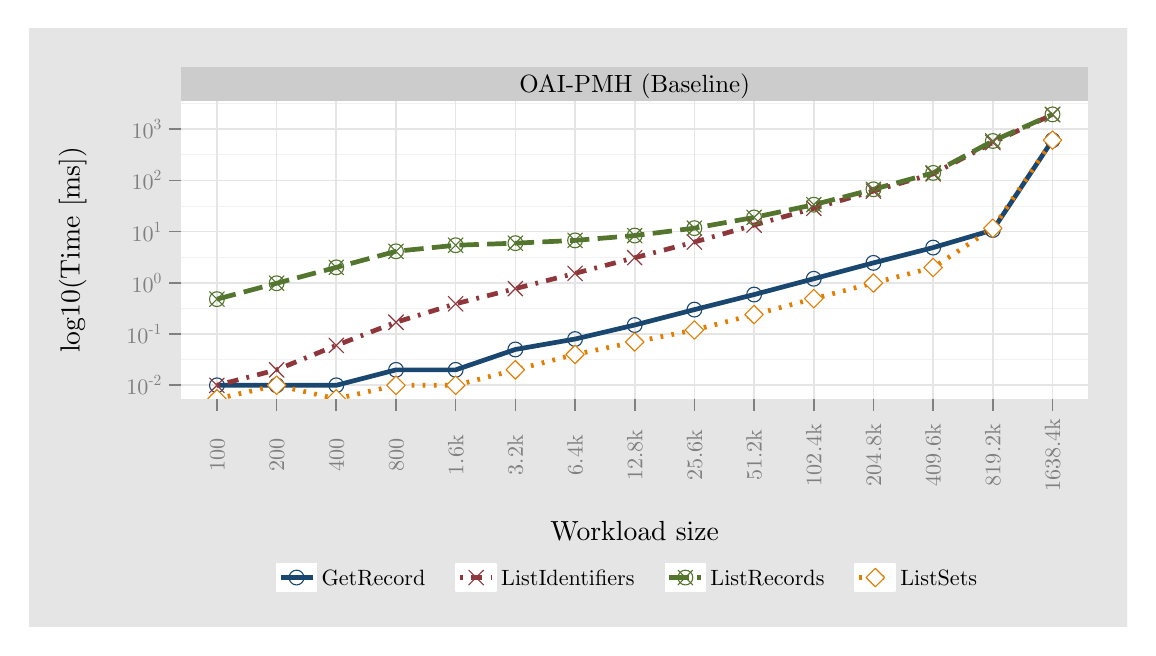
\begin{tikzpicture}[x=1pt,y=1pt]
\definecolor[named]{fillColor}{rgb}{1.00,1.00,1.00}
\path[use as bounding box,fill=fillColor,fill opacity=0.00] (0,0) rectangle (397.48,216.81);
\begin{scope}
\path[clip] (  0.00,  0.00) rectangle (397.48,216.81);
\definecolor[named]{drawColor}{rgb}{1.00,1.00,1.00}
\definecolor[named]{fillColor}{rgb}{0.90,0.90,0.90}

\path[draw=drawColor,line width= 0.6pt,line join=round,line cap=round,fill=fillColor] (  0.00,  0.00) rectangle (397.48,216.81);
\end{scope}
\begin{scope}
\path[clip] ( 55.45, 82.69) rectangle (383.26,190.36);
\definecolor[named]{fillColor}{rgb}{1.00,1.00,1.00}

\path[fill=fillColor] ( 55.45, 82.69) rectangle (383.26,190.36);
\definecolor[named]{drawColor}{rgb}{0.95,0.95,0.95}

\path[draw=drawColor,line width= 0.3pt,line join=round] ( 55.45, 96.84) --
	(383.26, 96.84);

\path[draw=drawColor,line width= 0.3pt,line join=round] ( 55.45,115.36) --
	(383.26,115.36);

\path[draw=drawColor,line width= 0.3pt,line join=round] ( 55.45,133.87) --
	(383.26,133.87);

\path[draw=drawColor,line width= 0.3pt,line join=round] ( 55.45,152.38) --
	(383.26,152.38);

\path[draw=drawColor,line width= 0.3pt,line join=round] ( 55.45,170.90) --
	(383.26,170.90);

\path[draw=drawColor,line width= 0.3pt,line join=round] ( 55.45,189.41) --
	(383.26,189.41);
\definecolor[named]{drawColor}{rgb}{0.90,0.90,0.90}

\path[draw=drawColor,line width= 0.6pt,line join=round] ( 55.45, 87.58) --
	(383.26, 87.58);

\path[draw=drawColor,line width= 0.6pt,line join=round] ( 55.45,106.10) --
	(383.26,106.10);

\path[draw=drawColor,line width= 0.6pt,line join=round] ( 55.45,124.61) --
	(383.26,124.61);

\path[draw=drawColor,line width= 0.6pt,line join=round] ( 55.45,143.13) --
	(383.26,143.13);

\path[draw=drawColor,line width= 0.6pt,line join=round] ( 55.45,161.64) --
	(383.26,161.64);

\path[draw=drawColor,line width= 0.6pt,line join=round] ( 55.45,180.15) --
	(383.26,180.15);

\path[draw=drawColor,line width= 0.6pt,line join=round] ( 68.39, 82.69) --
	( 68.39,190.36);

\path[draw=drawColor,line width= 0.6pt,line join=round] ( 89.95, 82.69) --
	( 89.95,190.36);

\path[draw=drawColor,line width= 0.6pt,line join=round] (111.52, 82.69) --
	(111.52,190.36);

\path[draw=drawColor,line width= 0.6pt,line join=round] (133.09, 82.69) --
	(133.09,190.36);

\path[draw=drawColor,line width= 0.6pt,line join=round] (154.65, 82.69) --
	(154.65,190.36);

\path[draw=drawColor,line width= 0.6pt,line join=round] (176.22, 82.69) --
	(176.22,190.36);

\path[draw=drawColor,line width= 0.6pt,line join=round] (197.79, 82.69) --
	(197.79,190.36);

\path[draw=drawColor,line width= 0.6pt,line join=round] (219.35, 82.69) --
	(219.35,190.36);

\path[draw=drawColor,line width= 0.6pt,line join=round] (240.92, 82.69) --
	(240.92,190.36);

\path[draw=drawColor,line width= 0.6pt,line join=round] (262.49, 82.69) --
	(262.49,190.36);

\path[draw=drawColor,line width= 0.6pt,line join=round] (284.05, 82.69) --
	(284.05,190.36);

\path[draw=drawColor,line width= 0.6pt,line join=round] (305.62, 82.69) --
	(305.62,190.36);

\path[draw=drawColor,line width= 0.6pt,line join=round] (327.19, 82.69) --
	(327.19,190.36);

\path[draw=drawColor,line width= 0.6pt,line join=round] (348.75, 82.69) --
	(348.75,190.36);

\path[draw=drawColor,line width= 0.6pt,line join=round] (370.32, 82.69) --
	(370.32,190.36);
\definecolor[named]{drawColor}{rgb}{0.10,0.28,0.44}

\path[draw=drawColor,line width= 1.7pt,line join=round] ( 68.39, 87.58) --
	( 89.95, 87.58) --
	(111.52, 87.58) --
	(133.09, 93.16) --
	(154.65, 93.16) --
	(176.22,100.53) --
	(197.79,104.30) --
	(219.35,109.36) --
	(240.92,114.93) --
	(262.49,120.37) --
	(284.05,126.08) --
	(305.62,131.82) --
	(327.19,137.34) --
	(348.75,143.68) --
	(370.32,176.15);
\definecolor[named]{drawColor}{rgb}{0.56,0.21,0.23}

\path[draw=drawColor,line width= 1.7pt,dash pattern=on 1pt off 3pt on 4pt off 3pt ,line join=round] ( 68.39, 87.58) --
	( 89.95, 93.16) --
	(111.52,101.99) --
	(133.09,110.36) --
	(154.65,117.04) --
	(176.22,122.51) --
	(197.79,128.03) --
	(219.35,133.68) --
	(240.92,139.35) --
	(262.49,145.47) --
	(284.05,151.53) --
	(305.62,157.78) --
	(327.19,163.99) --
	(348.75,175.32) --
	(370.32,185.41);
\definecolor[named]{drawColor}{rgb}{0.33,0.46,0.18}

\path[draw=drawColor,line width= 1.7pt,dash pattern=on 7pt off 3pt ,line join=round] ( 68.39,118.71) --
	( 89.95,124.45) --
	(111.52,130.19) --
	(133.09,136.00) --
	(154.65,138.19) --
	(176.22,138.94) --
	(197.79,139.94) --
	(219.35,141.69) --
	(240.92,144.37) --
	(262.49,148.24) --
	(284.05,152.84) --
	(305.62,158.41) --
	(327.19,164.33) --
	(348.75,175.86) --
	(370.32,185.47);
\definecolor[named]{drawColor}{rgb}{0.89,0.49,0.00}

\path[draw=drawColor,line width= 1.7pt,dash pattern=on 1pt off 3pt ,line join=round] ( 68.39, 82.69) --
	( 89.95, 87.58) --
	(111.52, 82.69) --
	(133.09, 87.58) --
	(154.65, 87.58) --
	(176.22, 93.16) --
	(197.79, 98.73) --
	(219.35,103.23) --
	(240.92,107.56) --
	(262.49,113.14) --
	(284.05,118.88) --
	(305.62,124.53) --
	(327.19,130.14) --
	(348.75,144.33) --
	(370.32,176.17);
\definecolor[named]{drawColor}{rgb}{0.10,0.28,0.44}

\path[draw=drawColor,line width= 0.4pt,line join=round,line cap=round] ( 68.39, 87.58) circle (  2.67);

\path[draw=drawColor,line width= 0.4pt,line join=round,line cap=round] ( 89.95, 87.58) circle (  2.67);

\path[draw=drawColor,line width= 0.4pt,line join=round,line cap=round] (111.52, 87.58) circle (  2.67);

\path[draw=drawColor,line width= 0.4pt,line join=round,line cap=round] (133.09, 93.16) circle (  2.67);

\path[draw=drawColor,line width= 0.4pt,line join=round,line cap=round] (154.65, 93.16) circle (  2.67);

\path[draw=drawColor,line width= 0.4pt,line join=round,line cap=round] (176.22,100.53) circle (  2.67);

\path[draw=drawColor,line width= 0.4pt,line join=round,line cap=round] (197.79,104.30) circle (  2.67);

\path[draw=drawColor,line width= 0.4pt,line join=round,line cap=round] (219.35,109.36) circle (  2.67);

\path[draw=drawColor,line width= 0.4pt,line join=round,line cap=round] (240.92,114.93) circle (  2.67);

\path[draw=drawColor,line width= 0.4pt,line join=round,line cap=round] (262.49,120.37) circle (  2.67);

\path[draw=drawColor,line width= 0.4pt,line join=round,line cap=round] (284.05,126.08) circle (  2.67);

\path[draw=drawColor,line width= 0.4pt,line join=round,line cap=round] (305.62,131.82) circle (  2.67);

\path[draw=drawColor,line width= 0.4pt,line join=round,line cap=round] (327.19,137.34) circle (  2.67);

\path[draw=drawColor,line width= 0.4pt,line join=round,line cap=round] (348.75,143.68) circle (  2.67);

\path[draw=drawColor,line width= 0.4pt,line join=round,line cap=round] (370.32,176.15) circle (  2.67);
\definecolor[named]{drawColor}{rgb}{0.56,0.21,0.23}

\path[draw=drawColor,line width= 0.4pt,line join=round,line cap=round,fill=fillColor] ( 65.72, 84.92) -- ( 71.06, 90.25);

\path[draw=drawColor,line width= 0.4pt,line join=round,line cap=round,fill=fillColor] ( 65.72, 90.25) -- ( 71.06, 84.92);

\path[draw=drawColor,line width= 0.4pt,line join=round,line cap=round,fill=fillColor] ( 87.29, 90.49) -- ( 92.62, 95.83);

\path[draw=drawColor,line width= 0.4pt,line join=round,line cap=round,fill=fillColor] ( 87.29, 95.83) -- ( 92.62, 90.49);

\path[draw=drawColor,line width= 0.4pt,line join=round,line cap=round,fill=fillColor] (108.85, 99.32) -- (114.19,104.66);

\path[draw=drawColor,line width= 0.4pt,line join=round,line cap=round,fill=fillColor] (108.85,104.66) -- (114.19, 99.32);

\path[draw=drawColor,line width= 0.4pt,line join=round,line cap=round,fill=fillColor] (130.42,107.70) -- (135.76,113.03);

\path[draw=drawColor,line width= 0.4pt,line join=round,line cap=round,fill=fillColor] (130.42,113.03) -- (135.76,107.70);

\path[draw=drawColor,line width= 0.4pt,line join=round,line cap=round,fill=fillColor] (151.99,114.37) -- (157.32,119.71);

\path[draw=drawColor,line width= 0.4pt,line join=round,line cap=round,fill=fillColor] (151.99,119.71) -- (157.32,114.37);

\path[draw=drawColor,line width= 0.4pt,line join=round,line cap=round,fill=fillColor] (173.55,119.84) -- (178.89,125.18);

\path[draw=drawColor,line width= 0.4pt,line join=round,line cap=round,fill=fillColor] (173.55,125.18) -- (178.89,119.84);

\path[draw=drawColor,line width= 0.4pt,line join=round,line cap=round,fill=fillColor] (195.12,125.36) -- (200.45,130.70);

\path[draw=drawColor,line width= 0.4pt,line join=round,line cap=round,fill=fillColor] (195.12,130.70) -- (200.45,125.36);

\path[draw=drawColor,line width= 0.4pt,line join=round,line cap=round,fill=fillColor] (216.69,131.02) -- (222.02,136.35);

\path[draw=drawColor,line width= 0.4pt,line join=round,line cap=round,fill=fillColor] (216.69,136.35) -- (222.02,131.02);

\path[draw=drawColor,line width= 0.4pt,line join=round,line cap=round,fill=fillColor] (238.25,136.68) -- (243.59,142.01);

\path[draw=drawColor,line width= 0.4pt,line join=round,line cap=round,fill=fillColor] (238.25,142.01) -- (243.59,136.68);

\path[draw=drawColor,line width= 0.4pt,line join=round,line cap=round,fill=fillColor] (259.82,142.80) -- (265.15,148.13);

\path[draw=drawColor,line width= 0.4pt,line join=round,line cap=round,fill=fillColor] (259.82,148.13) -- (265.15,142.80);

\path[draw=drawColor,line width= 0.4pt,line join=round,line cap=round,fill=fillColor] (281.39,148.87) -- (286.72,154.20);

\path[draw=drawColor,line width= 0.4pt,line join=round,line cap=round,fill=fillColor] (281.39,154.20) -- (286.72,148.87);

\path[draw=drawColor,line width= 0.4pt,line join=round,line cap=round,fill=fillColor] (302.95,155.11) -- (308.29,160.44);

\path[draw=drawColor,line width= 0.4pt,line join=round,line cap=round,fill=fillColor] (302.95,160.44) -- (308.29,155.11);

\path[draw=drawColor,line width= 0.4pt,line join=round,line cap=round,fill=fillColor] (324.52,161.32) -- (329.85,166.66);

\path[draw=drawColor,line width= 0.4pt,line join=round,line cap=round,fill=fillColor] (324.52,166.66) -- (329.85,161.32);

\path[draw=drawColor,line width= 0.4pt,line join=round,line cap=round,fill=fillColor] (346.08,172.65) -- (351.42,177.98);

\path[draw=drawColor,line width= 0.4pt,line join=round,line cap=round,fill=fillColor] (346.08,177.98) -- (351.42,172.65);

\path[draw=drawColor,line width= 0.4pt,line join=round,line cap=round,fill=fillColor] (367.65,182.74) -- (372.99,188.08);

\path[draw=drawColor,line width= 0.4pt,line join=round,line cap=round,fill=fillColor] (367.65,188.08) -- (372.99,182.74);
\definecolor[named]{drawColor}{rgb}{0.33,0.46,0.18}

\path[draw=drawColor,line width= 0.4pt,line join=round,line cap=round] ( 68.39,118.71) circle (  2.67);

\path[draw=drawColor,line width= 0.4pt,line join=round,line cap=round] ( 65.72,116.04) -- ( 71.06,121.38);

\path[draw=drawColor,line width= 0.4pt,line join=round,line cap=round] ( 65.72,121.38) -- ( 71.06,116.04);

\path[draw=drawColor,line width= 0.4pt,line join=round,line cap=round] ( 89.95,124.45) circle (  2.67);

\path[draw=drawColor,line width= 0.4pt,line join=round,line cap=round] ( 87.29,121.78) -- ( 92.62,127.12);

\path[draw=drawColor,line width= 0.4pt,line join=round,line cap=round] ( 87.29,127.12) -- ( 92.62,121.78);

\path[draw=drawColor,line width= 0.4pt,line join=round,line cap=round] (111.52,130.19) circle (  2.67);

\path[draw=drawColor,line width= 0.4pt,line join=round,line cap=round] (108.85,127.52) -- (114.19,132.85);

\path[draw=drawColor,line width= 0.4pt,line join=round,line cap=round] (108.85,132.85) -- (114.19,127.52);

\path[draw=drawColor,line width= 0.4pt,line join=round,line cap=round] (133.09,136.00) circle (  2.67);

\path[draw=drawColor,line width= 0.4pt,line join=round,line cap=round] (130.42,133.33) -- (135.76,138.66);

\path[draw=drawColor,line width= 0.4pt,line join=round,line cap=round] (130.42,138.66) -- (135.76,133.33);

\path[draw=drawColor,line width= 0.4pt,line join=round,line cap=round] (154.65,138.19) circle (  2.67);

\path[draw=drawColor,line width= 0.4pt,line join=round,line cap=round] (151.99,135.52) -- (157.32,140.85);

\path[draw=drawColor,line width= 0.4pt,line join=round,line cap=round] (151.99,140.85) -- (157.32,135.52);

\path[draw=drawColor,line width= 0.4pt,line join=round,line cap=round] (176.22,138.94) circle (  2.67);

\path[draw=drawColor,line width= 0.4pt,line join=round,line cap=round] (173.55,136.27) -- (178.89,141.60);

\path[draw=drawColor,line width= 0.4pt,line join=round,line cap=round] (173.55,141.60) -- (178.89,136.27);

\path[draw=drawColor,line width= 0.4pt,line join=round,line cap=round] (197.79,139.94) circle (  2.67);

\path[draw=drawColor,line width= 0.4pt,line join=round,line cap=round] (195.12,137.27) -- (200.45,142.61);

\path[draw=drawColor,line width= 0.4pt,line join=round,line cap=round] (195.12,142.61) -- (200.45,137.27);

\path[draw=drawColor,line width= 0.4pt,line join=round,line cap=round] (219.35,141.69) circle (  2.67);

\path[draw=drawColor,line width= 0.4pt,line join=round,line cap=round] (216.69,139.03) -- (222.02,144.36);

\path[draw=drawColor,line width= 0.4pt,line join=round,line cap=round] (216.69,144.36) -- (222.02,139.03);

\path[draw=drawColor,line width= 0.4pt,line join=round,line cap=round] (240.92,144.37) circle (  2.67);

\path[draw=drawColor,line width= 0.4pt,line join=round,line cap=round] (238.25,141.71) -- (243.59,147.04);

\path[draw=drawColor,line width= 0.4pt,line join=round,line cap=round] (238.25,147.04) -- (243.59,141.71);

\path[draw=drawColor,line width= 0.4pt,line join=round,line cap=round] (262.49,148.24) circle (  2.67);

\path[draw=drawColor,line width= 0.4pt,line join=round,line cap=round] (259.82,145.58) -- (265.15,150.91);

\path[draw=drawColor,line width= 0.4pt,line join=round,line cap=round] (259.82,150.91) -- (265.15,145.58);

\path[draw=drawColor,line width= 0.4pt,line join=round,line cap=round] (284.05,152.84) circle (  2.67);

\path[draw=drawColor,line width= 0.4pt,line join=round,line cap=round] (281.39,150.17) -- (286.72,155.50);

\path[draw=drawColor,line width= 0.4pt,line join=round,line cap=round] (281.39,155.50) -- (286.72,150.17);

\path[draw=drawColor,line width= 0.4pt,line join=round,line cap=round] (305.62,158.41) circle (  2.67);

\path[draw=drawColor,line width= 0.4pt,line join=round,line cap=round] (302.95,155.75) -- (308.29,161.08);

\path[draw=drawColor,line width= 0.4pt,line join=round,line cap=round] (302.95,161.08) -- (308.29,155.75);

\path[draw=drawColor,line width= 0.4pt,line join=round,line cap=round] (327.19,164.33) circle (  2.67);

\path[draw=drawColor,line width= 0.4pt,line join=round,line cap=round] (324.52,161.66) -- (329.85,167.00);

\path[draw=drawColor,line width= 0.4pt,line join=round,line cap=round] (324.52,167.00) -- (329.85,161.66);

\path[draw=drawColor,line width= 0.4pt,line join=round,line cap=round] (348.75,175.86) circle (  2.67);

\path[draw=drawColor,line width= 0.4pt,line join=round,line cap=round] (346.08,173.19) -- (351.42,178.53);

\path[draw=drawColor,line width= 0.4pt,line join=round,line cap=round] (346.08,178.53) -- (351.42,173.19);

\path[draw=drawColor,line width= 0.4pt,line join=round,line cap=round] (370.32,185.47) circle (  2.67);

\path[draw=drawColor,line width= 0.4pt,line join=round,line cap=round] (367.65,182.80) -- (372.99,188.14);

\path[draw=drawColor,line width= 0.4pt,line join=round,line cap=round] (367.65,188.14) -- (372.99,182.80);
\definecolor[named]{drawColor}{rgb}{0.89,0.49,0.00}

\path[draw=drawColor,line width= 0.4pt,line join=round,line cap=round,fill=fillColor] ( 68.39, 79.35) --
	( 71.73, 82.69) --
	( 68.39, 86.03) --
	( 65.05, 82.69) --
	cycle;

\path[draw=drawColor,line width= 0.4pt,line join=round,line cap=round,fill=fillColor] ( 89.95, 84.24) --
	( 93.30, 87.58) --
	( 89.95, 90.93) --
	( 86.61, 87.58) --
	cycle;

\path[draw=drawColor,line width= 0.4pt,line join=round,line cap=round,fill=fillColor] (111.52, 79.35) --
	(114.86, 82.69) --
	(111.52, 86.03) --
	(108.18, 82.69) --
	cycle;

\path[draw=drawColor,line width= 0.4pt,line join=round,line cap=round,fill=fillColor] (133.09, 84.24) --
	(136.43, 87.58) --
	(133.09, 90.93) --
	(129.74, 87.58) --
	cycle;

\path[draw=drawColor,line width= 0.4pt,line join=round,line cap=round,fill=fillColor] (154.65, 84.24) --
	(158.00, 87.58) --
	(154.65, 90.93) --
	(151.31, 87.58) --
	cycle;

\path[draw=drawColor,line width= 0.4pt,line join=round,line cap=round,fill=fillColor] (176.22, 89.81) --
	(179.56, 93.16) --
	(176.22, 96.50) --
	(172.88, 93.16) --
	cycle;

\path[draw=drawColor,line width= 0.4pt,line join=round,line cap=round,fill=fillColor] (197.79, 95.39) --
	(201.13, 98.73) --
	(197.79,102.07) --
	(194.44, 98.73) --
	cycle;

\path[draw=drawColor,line width= 0.4pt,line join=round,line cap=round,fill=fillColor] (219.35, 99.89) --
	(222.70,103.23) --
	(219.35,106.57) --
	(216.01,103.23) --
	cycle;

\path[draw=drawColor,line width= 0.4pt,line join=round,line cap=round,fill=fillColor] (240.92,104.22) --
	(244.26,107.56) --
	(240.92,110.91) --
	(237.58,107.56) --
	cycle;

\path[draw=drawColor,line width= 0.4pt,line join=round,line cap=round,fill=fillColor] (262.49,109.79) --
	(265.83,113.14) --
	(262.49,116.48) --
	(259.14,113.14) --
	cycle;

\path[draw=drawColor,line width= 0.4pt,line join=round,line cap=round,fill=fillColor] (284.05,115.53) --
	(287.40,118.88) --
	(284.05,122.22) --
	(280.71,118.88) --
	cycle;

\path[draw=drawColor,line width= 0.4pt,line join=round,line cap=round,fill=fillColor] (305.62,121.19) --
	(308.96,124.53) --
	(305.62,127.87) --
	(302.28,124.53) --
	cycle;

\path[draw=drawColor,line width= 0.4pt,line join=round,line cap=round,fill=fillColor] (327.19,126.80) --
	(330.53,130.14) --
	(327.19,133.49) --
	(323.84,130.14) --
	cycle;

\path[draw=drawColor,line width= 0.4pt,line join=round,line cap=round,fill=fillColor] (348.75,140.98) --
	(352.10,144.33) --
	(348.75,147.67) --
	(345.41,144.33) --
	cycle;

\path[draw=drawColor,line width= 0.4pt,line join=round,line cap=round,fill=fillColor] (370.32,172.82) --
	(373.66,176.17) --
	(370.32,179.51) --
	(366.98,176.17) --
	cycle;
\end{scope}
\begin{scope}
\path[clip] (  0.00,  0.00) rectangle (397.48,216.81);
\definecolor[named]{fillColor}{rgb}{0.80,0.80,0.80}

\path[fill=fillColor] ( 55.45,190.36) rectangle (383.26,202.58);
\definecolor[named]{drawColor}{rgb}{0.00,0.00,0.00}

\node[text=drawColor,anchor=base,inner sep=0pt, outer sep=0pt, scale=  0.90] at (219.35,193.37) {OAI-PMH (Baseline)};
\end{scope}
\begin{scope}
\path[clip] (  0.00,  0.00) rectangle (397.48,216.81);
\definecolor[named]{drawColor}{rgb}{0.50,0.50,0.50}

\node[text=drawColor,anchor=base west,inner sep=0pt, outer sep=0pt, scale=  0.80] at ( 35.67, 84.15) {10};

\node[text=drawColor,anchor=base west,inner sep=0pt, outer sep=0pt, scale=  0.56] at ( 43.67, 87.42) {-};

\node[text=drawColor,anchor=base west,inner sep=0pt, outer sep=0pt, scale=  0.56] at ( 45.54, 87.42) {2};

\node[text=drawColor,anchor=base west,inner sep=0pt, outer sep=0pt, scale=  0.80] at ( 35.67,102.67) {10};

\node[text=drawColor,anchor=base west,inner sep=0pt, outer sep=0pt, scale=  0.56] at ( 43.67,105.94) {-};

\node[text=drawColor,anchor=base west,inner sep=0pt, outer sep=0pt, scale=  0.56] at ( 45.54,105.94) {1};

\node[text=drawColor,anchor=base west,inner sep=0pt, outer sep=0pt, scale=  0.80] at ( 37.54,121.18) {10};

\node[text=drawColor,anchor=base west,inner sep=0pt, outer sep=0pt, scale=  0.56] at ( 45.54,124.45) {0};

\node[text=drawColor,anchor=base west,inner sep=0pt, outer sep=0pt, scale=  0.80] at ( 37.54,139.69) {10};

\node[text=drawColor,anchor=base west,inner sep=0pt, outer sep=0pt, scale=  0.56] at ( 45.54,142.96) {1};

\node[text=drawColor,anchor=base west,inner sep=0pt, outer sep=0pt, scale=  0.80] at ( 37.54,158.21) {10};

\node[text=drawColor,anchor=base west,inner sep=0pt, outer sep=0pt, scale=  0.56] at ( 45.54,161.48) {2};

\node[text=drawColor,anchor=base west,inner sep=0pt, outer sep=0pt, scale=  0.80] at ( 37.54,176.72) {10};

\node[text=drawColor,anchor=base west,inner sep=0pt, outer sep=0pt, scale=  0.56] at ( 45.54,179.99) {3};
\end{scope}
\begin{scope}
\path[clip] (  0.00,  0.00) rectangle (397.48,216.81);
\definecolor[named]{drawColor}{rgb}{0.50,0.50,0.50}

\path[draw=drawColor,line width= 0.6pt,line join=round] ( 51.18, 87.58) --
	( 55.45, 87.58);

\path[draw=drawColor,line width= 0.6pt,line join=round] ( 51.18,106.10) --
	( 55.45,106.10);

\path[draw=drawColor,line width= 0.6pt,line join=round] ( 51.18,124.61) --
	( 55.45,124.61);

\path[draw=drawColor,line width= 0.6pt,line join=round] ( 51.18,143.13) --
	( 55.45,143.13);

\path[draw=drawColor,line width= 0.6pt,line join=round] ( 51.18,161.64) --
	( 55.45,161.64);

\path[draw=drawColor,line width= 0.6pt,line join=round] ( 51.18,180.15) --
	( 55.45,180.15);
\end{scope}
\begin{scope}
\path[clip] (  0.00,  0.00) rectangle (397.48,216.81);
\definecolor[named]{drawColor}{rgb}{0.50,0.50,0.50}

\path[draw=drawColor,line width= 0.6pt,line join=round] ( 68.39, 78.42) --
	( 68.39, 82.69);

\path[draw=drawColor,line width= 0.6pt,line join=round] ( 89.95, 78.42) --
	( 89.95, 82.69);

\path[draw=drawColor,line width= 0.6pt,line join=round] (111.52, 78.42) --
	(111.52, 82.69);

\path[draw=drawColor,line width= 0.6pt,line join=round] (133.09, 78.42) --
	(133.09, 82.69);

\path[draw=drawColor,line width= 0.6pt,line join=round] (154.65, 78.42) --
	(154.65, 82.69);

\path[draw=drawColor,line width= 0.6pt,line join=round] (176.22, 78.42) --
	(176.22, 82.69);

\path[draw=drawColor,line width= 0.6pt,line join=round] (197.79, 78.42) --
	(197.79, 82.69);

\path[draw=drawColor,line width= 0.6pt,line join=round] (219.35, 78.42) --
	(219.35, 82.69);

\path[draw=drawColor,line width= 0.6pt,line join=round] (240.92, 78.42) --
	(240.92, 82.69);

\path[draw=drawColor,line width= 0.6pt,line join=round] (262.49, 78.42) --
	(262.49, 82.69);

\path[draw=drawColor,line width= 0.6pt,line join=round] (284.05, 78.42) --
	(284.05, 82.69);

\path[draw=drawColor,line width= 0.6pt,line join=round] (305.62, 78.42) --
	(305.62, 82.69);

\path[draw=drawColor,line width= 0.6pt,line join=round] (327.19, 78.42) --
	(327.19, 82.69);

\path[draw=drawColor,line width= 0.6pt,line join=round] (348.75, 78.42) --
	(348.75, 82.69);

\path[draw=drawColor,line width= 0.6pt,line join=round] (370.32, 78.42) --
	(370.32, 82.69);
\end{scope}
\begin{scope}
\path[clip] (  0.00,  0.00) rectangle (397.48,216.81);
\definecolor[named]{drawColor}{rgb}{0.50,0.50,0.50}

\node[text=drawColor,rotate= 90.00,anchor=base,inner sep=0pt, outer sep=0pt, scale=  0.80] at ( 71.14, 62.36) {100};

\node[text=drawColor,rotate= 90.00,anchor=base,inner sep=0pt, outer sep=0pt, scale=  0.80] at ( 92.71, 62.36) {200};

\node[text=drawColor,rotate= 90.00,anchor=base,inner sep=0pt, outer sep=0pt, scale=  0.80] at (114.28, 62.36) {400};

\node[text=drawColor,rotate= 90.00,anchor=base,inner sep=0pt, outer sep=0pt, scale=  0.80] at (135.84, 62.36) {800};

\node[text=drawColor,rotate= 90.00,anchor=base,inner sep=0pt, outer sep=0pt, scale=  0.80] at (157.41, 62.36) {1.6k};

\node[text=drawColor,rotate= 90.00,anchor=base,inner sep=0pt, outer sep=0pt, scale=  0.80] at (178.98, 62.36) {3.2k};

\node[text=drawColor,rotate= 90.00,anchor=base,inner sep=0pt, outer sep=0pt, scale=  0.80] at (200.54, 62.36) {6.4k};

\node[text=drawColor,rotate= 90.00,anchor=base,inner sep=0pt, outer sep=0pt, scale=  0.80] at (222.11, 62.36) {12.8k};

\node[text=drawColor,rotate= 90.00,anchor=base,inner sep=0pt, outer sep=0pt, scale=  0.80] at (243.67, 62.36) {25.6k};

\node[text=drawColor,rotate= 90.00,anchor=base,inner sep=0pt, outer sep=0pt, scale=  0.80] at (265.24, 62.36) {51.2k};

\node[text=drawColor,rotate= 90.00,anchor=base,inner sep=0pt, outer sep=0pt, scale=  0.80] at (286.81, 62.36) {102.4k};

\node[text=drawColor,rotate= 90.00,anchor=base,inner sep=0pt, outer sep=0pt, scale=  0.80] at (308.37, 62.36) {204.8k};

\node[text=drawColor,rotate= 90.00,anchor=base,inner sep=0pt, outer sep=0pt, scale=  0.80] at (329.94, 62.36) {409.6k};

\node[text=drawColor,rotate= 90.00,anchor=base,inner sep=0pt, outer sep=0pt, scale=  0.80] at (351.51, 62.36) {819.2k};

\node[text=drawColor,rotate= 90.00,anchor=base,inner sep=0pt, outer sep=0pt, scale=  0.80] at (373.07, 62.36) {1638.4k};
\end{scope}
\begin{scope}
\path[clip] (  0.00,  0.00) rectangle (397.48,216.81);
\definecolor[named]{drawColor}{rgb}{0.00,0.00,0.00}

\node[text=drawColor,anchor=base,inner sep=0pt, outer sep=0pt, scale=  1.00] at (219.35, 31.41) {Workload size};
\end{scope}
\begin{scope}
\path[clip] (  0.00,  0.00) rectangle (397.48,216.81);
\definecolor[named]{drawColor}{rgb}{0.00,0.00,0.00}

\node[text=drawColor,rotate= 90.00,anchor=base,inner sep=0pt, outer sep=0pt, scale=  1.00] at ( 18.80,136.53) {log10(Time [ms])};
\end{scope}
\begin{scope}
\path[clip] (  0.00,  0.00) rectangle (397.48,216.81);
\definecolor[named]{fillColor}{rgb}{0.90,0.90,0.90}

\path[fill=fillColor] ( 82.04,  8.87) rectangle (356.67, 27.36);
\end{scope}
\begin{scope}
\path[clip] (  0.00,  0.00) rectangle (397.48,216.81);
\definecolor[named]{drawColor}{rgb}{1.00,1.00,1.00}
\definecolor[named]{fillColor}{rgb}{1.00,1.00,1.00}

\path[draw=drawColor,line width= 0.6pt,line join=round,line cap=round,fill=fillColor] ( 89.92, 13.14) rectangle (104.38, 23.09);
\end{scope}
\begin{scope}
\path[clip] (  0.00,  0.00) rectangle (397.48,216.81);
\definecolor[named]{drawColor}{rgb}{0.10,0.28,0.44}

\path[draw=drawColor,line width= 1.7pt,line join=round] ( 91.37, 18.11) -- (102.93, 18.11);
\end{scope}
\begin{scope}
\path[clip] (  0.00,  0.00) rectangle (397.48,216.81);
\definecolor[named]{drawColor}{rgb}{0.10,0.28,0.44}

\path[draw=drawColor,line width= 0.4pt,line join=round,line cap=round] ( 97.15, 18.11) circle (  2.67);
\end{scope}
\begin{scope}
\path[clip] (  0.00,  0.00) rectangle (397.48,216.81);
\definecolor[named]{drawColor}{rgb}{1.00,1.00,1.00}
\definecolor[named]{fillColor}{rgb}{1.00,1.00,1.00}

\path[draw=drawColor,line width= 0.6pt,line join=round,line cap=round,fill=fillColor] (154.83, 13.14) rectangle (169.29, 23.09);
\end{scope}
\begin{scope}
\path[clip] (  0.00,  0.00) rectangle (397.48,216.81);
\definecolor[named]{drawColor}{rgb}{0.56,0.21,0.23}

\path[draw=drawColor,line width= 1.7pt,dash pattern=on 1pt off 3pt on 4pt off 3pt ,line join=round] (156.28, 18.11) -- (167.84, 18.11);
\end{scope}
\begin{scope}
\path[clip] (  0.00,  0.00) rectangle (397.48,216.81);
\definecolor[named]{drawColor}{rgb}{0.56,0.21,0.23}
\definecolor[named]{fillColor}{rgb}{1.00,1.00,1.00}

\path[draw=drawColor,line width= 0.4pt,line join=round,line cap=round,fill=fillColor] (159.39, 15.45) -- (164.73, 20.78);

\path[draw=drawColor,line width= 0.4pt,line join=round,line cap=round,fill=fillColor] (159.39, 20.78) -- (164.73, 15.45);
\end{scope}
\begin{scope}
\path[clip] (  0.00,  0.00) rectangle (397.48,216.81);
\definecolor[named]{drawColor}{rgb}{1.00,1.00,1.00}
\definecolor[named]{fillColor}{rgb}{1.00,1.00,1.00}

\path[draw=drawColor,line width= 0.6pt,line join=round,line cap=round,fill=fillColor] (230.45, 13.14) rectangle (244.90, 23.09);
\end{scope}
\begin{scope}
\path[clip] (  0.00,  0.00) rectangle (397.48,216.81);
\definecolor[named]{drawColor}{rgb}{0.33,0.46,0.18}

\path[draw=drawColor,line width= 1.7pt,dash pattern=on 7pt off 3pt ,line join=round] (231.89, 18.11) -- (243.45, 18.11);
\end{scope}
\begin{scope}
\path[clip] (  0.00,  0.00) rectangle (397.48,216.81);
\definecolor[named]{drawColor}{rgb}{0.33,0.46,0.18}

\path[draw=drawColor,line width= 0.4pt,line join=round,line cap=round] (237.67, 18.11) circle (  2.67);

\path[draw=drawColor,line width= 0.4pt,line join=round,line cap=round] (235.00, 15.45) -- (240.34, 20.78);

\path[draw=drawColor,line width= 0.4pt,line join=round,line cap=round] (235.00, 20.78) -- (240.34, 15.45);
\end{scope}
\begin{scope}
\path[clip] (  0.00,  0.00) rectangle (397.48,216.81);
\definecolor[named]{drawColor}{rgb}{1.00,1.00,1.00}
\definecolor[named]{fillColor}{rgb}{1.00,1.00,1.00}

\path[draw=drawColor,line width= 0.6pt,line join=round,line cap=round,fill=fillColor] (299.06, 13.14) rectangle (313.51, 23.09);
\end{scope}
\begin{scope}
\path[clip] (  0.00,  0.00) rectangle (397.48,216.81);
\definecolor[named]{drawColor}{rgb}{0.89,0.49,0.00}

\path[draw=drawColor,line width= 1.7pt,dash pattern=on 1pt off 3pt ,line join=round] (300.50, 18.11) -- (312.07, 18.11);
\end{scope}
\begin{scope}
\path[clip] (  0.00,  0.00) rectangle (397.48,216.81);
\definecolor[named]{drawColor}{rgb}{0.89,0.49,0.00}
\definecolor[named]{fillColor}{rgb}{1.00,1.00,1.00}

\path[draw=drawColor,line width= 0.4pt,line join=round,line cap=round,fill=fillColor] (306.28, 14.77) --
	(309.63, 18.11) --
	(306.28, 21.46) --
	(302.94, 18.11) --
	cycle;
\end{scope}
\begin{scope}
\path[clip] (  0.00,  0.00) rectangle (397.48,216.81);
\definecolor[named]{drawColor}{rgb}{0.00,0.00,0.00}

\node[text=drawColor,anchor=base west,inner sep=0pt, outer sep=0pt, scale=  0.80] at (106.18, 15.36) {GetRecord $\;\;\;$};
\end{scope}
\begin{scope}
\path[clip] (  0.00,  0.00) rectangle (397.48,216.81);
\definecolor[named]{drawColor}{rgb}{0.00,0.00,0.00}

\node[text=drawColor,anchor=base west,inner sep=0pt, outer sep=0pt, scale=  0.80] at (171.10, 15.36) {ListIdentifiers $\;\;\;$};
\end{scope}
\begin{scope}
\path[clip] (  0.00,  0.00) rectangle (397.48,216.81);
\definecolor[named]{drawColor}{rgb}{0.00,0.00,0.00}

\node[text=drawColor,anchor=base west,inner sep=0pt, outer sep=0pt, scale=  0.80] at (246.71, 15.36) {ListRecords $\;\;\;$};
\end{scope}
\begin{scope}
\path[clip] (  0.00,  0.00) rectangle (397.48,216.81);
\definecolor[named]{drawColor}{rgb}{0.00,0.00,0.00}

\node[text=drawColor,anchor=base west,inner sep=0pt, outer sep=0pt, scale=  0.80] at (315.32, 15.36) {ListSets $\;\;\;$};
\end{scope}
\end{tikzpicture}

 }
 \caption[Baseline performance benchmarks for OAI-PMH data provider]{OAI-PMH data provider\index{OAI-PMH!Data Provider} baseline performance benchmarks results for all four request verbs.}
 \label{fig:experimentation:performance:oaipmh:verbs-baseline}
\end{figure}


\subparagraph{Discussion}

The ListRecords\index{OAI-PMH!Verbs!ListRecords} and ListIdentifiers\index{OAI-PMH!Verbs!ListIdentifiers} verbs are the most expensive of the OAI-PMH verbs, each taking more than \num{2} seconds when the workload\index{Workload} size goes beyond \num{400} and \num{6400} respectively. In contrast, the GetRecord\index{OAI-PMH!Verbs!GetRecord} and ListSets\index{OAI-PMH!Verbs!ListSets} verbs only go beyond acceptable limits when the workload\index{Workload} size exceeds \num{204800} and \num{819200} respectively. 

\paragraph{Experiment: Impact of collection structure}
\label{sec:evaluation:performance:oaipmh-data-provider:experiment2}

The results obtained from the baseline experiment conducted in Experiment 1
involved the use of a one-level collection structure illustrated in Figure~\ref{fig:experimentation:performance:workload-design:directory-structures:dataset1}. This experiment was
conducted to assess the impact that a multi-level structure would have on the
overall performance of an OAI-PMH data provider\index{OAI-PMH!Data Provider} whilst varying the workload.

\subparagraph{Methodology} %\hspace*{\fill} \\ % provision for dirtree

A three-level collection structure, shown in Figure~\ref{fig:experimentation:performance:workload-design:directory-structures:dataset3}, was used. Siege was then used to to simulate a single user request with a total of 5 repeated runs for GetRecord, ListIdentifiers, ListRecords\index{OAI-PMH!Verbs!ListRecords} and ListSets\index{OAI-PMH!Verbs!ListSets} verbs; the average response times for each case were then recorded.

\subparagraph{Results}

Figure~\ref{fig:experimentation:performance:oaipmh:level} show results of the impact on performance of collection structure on the OAI-PMH verbs.

% 
% Already available in appendices
\begin{comment}
\tablespacing
%\begin{longtable}{p{0.12\linewidth} p{0.12\linewidth} p{0.12\linewidth}
%p{0.12\linewidth} p{0.12\linewidth} p{0.12\linewidth} p{0.12\linewidth}}
%%\begin{longtable}{ccccccc}
\begin{longtable}{
>{\arraybackslash}m{0.07\linewidth}|
>{\centering\arraybackslash}m{0.11\linewidth}|
>{\centering\arraybackslash}m{0.11\linewidth}|
>{\centering\arraybackslash}m{0.11\linewidth}|
>{\centering\arraybackslash}m{0.11\linewidth}|
>{\centering\arraybackslash}m{0.11\linewidth}|
>{\centering\arraybackslash}m{0.11\linewidth}}

\caption{ListRecords response times for varying workload structures}
\label{tab:experimentation:performance:oaipmh:level} \\

 %%%%%\toprule
 \hline
 %%%%%{} & 
 %%%%%\multicolumn{6}{c}{\textbf\textbf{Workload Structure}}\\
 %%%%%\midrule
 %%%%%\hline
 {} & 
 \multicolumn{2}{c|}{\textbf{Dataset \#1}} &  
 \multicolumn{2}{c|}{\textbf{Dataset \#2}} &
 \multicolumn{2}{c}{\textbf{Dataset \#3}}\\
 %%%%%\midrule
 \cline{2-7}
 {} & 
 {\begin{sideways}\textbf{Listset 1}\end{sideways}} & 
 {\begin{sideways}\textbf{Listset N}\end{sideways}} &
 {\begin{sideways}\textbf{Listset 1}\end{sideways}} & 
 {\begin{sideways}\textbf{Listset N}\end{sideways}} &
 {\begin{sideways}\textbf{Listset 1}\end{sideways}} & 
 {\begin{sideways}\textbf{Listset N}\end{sideways}} \\
 %%%%%\midrule
 \hline \hline
 \endfirsthead

 \caption[]{(continued)}\\
 %%%%%\toprule
 \hline
 %%%%%{} & 
 %%%%%\multicolumn{6}{c}{\textbf\textbf{Workload Structure}}\\
 %%%%%\midrule
 %%%%%\hline
 {} & 
 \multicolumn{2}{c|}{\textbf{Dataset \#1}} &  
 \multicolumn{2}{c|}{\textbf{Dataset \#2}} &
 \multicolumn{2}{c}{\textbf{Dataset \#3}}\\
 %%%%%\midrule
 \cline{2-7}
 {} &
 {\begin{sideways}\textbf{Listset 1}\end{sideways}} & 
 {\begin{sideways}\textbf{Listset N}\end{sideways}} &
 {\begin{sideways}\textbf{Listset 1}\end{sideways}} & 
 {\begin{sideways}\textbf{Listset N}\end{sideways}} &
 {\begin{sideways}\textbf{Listset 1}\end{sideways}} & 
 {\begin{sideways}\textbf{Listset N}\end{sideways}} \\
 %%%%%\midrule
 \hline \hline
 \endhead

 % Page footer
 %%%%%\midrule
 \hline
 \multicolumn{7}{r}{(Continued on next page)} \\
 \endfoot

 % Last page footer
 \bottomrule
 \endlastfoot

 \textbf{W1} & {\tablenum[table-format=7]{490}} & {--} & {\tablenum[table-format=7]{490}} & {--} & {\tablenum[table-format=7]{490}} & {--} \\ 
 \textbf{W2} & {\tablenum[table-format=7]{980}} & {--} & {\tablenum[table-format=7]{980}} & {--} & {\tablenum[table-format=7]{980}} & {--} \\ 
 \textbf{W3} & {\tablenum[table-format=7]{1980}} & {--} & {\tablenum[table-format=7]{2010}} & {--} & {\tablenum[table-format=7]{2010}} & {--} \\ 
 \textbf{W4} & {\tablenum[table-format=7]{4080}} & {--} & {\tablenum[table-format=7]{4140}} & {--} & {\tablenum[table-format=7]{4120}} & {--} \\ 
 \textbf{W5} & {\tablenum[table-format=7]{5410}} & {\tablenum[table-format=7]{3390}} & {\tablenum[table-format=7]{5510}} & {\tablenum[table-format=7]{3440}} & {\tablenum[table-format=7]{5460}} & {\tablenum[table-format=7]{3400}} \\ 
 \textbf{W6} & {\tablenum[table-format=7]{5910}} & {\tablenum[table-format=7]{6010}} & {\tablenum[table-format=7]{6010}} & {\tablenum[table-format=7]{6120}} & {\tablenum[table-format=7]{5960}} & {\tablenum[table-format=7]{6040}} \\ 
 \textbf{W7} & {\tablenum[table-format=7]{6720}} & {\tablenum[table-format=7]{6890}} & {\tablenum[table-format=7]{6940}} & {\tablenum[table-format=7]{7020}} & {\tablenum[table-format=7]{6780}} & {\tablenum[table-format=7]{6930}} \\ 
 \textbf{W8} & {\tablenum[table-format=7]{8440}} & {\tablenum[table-format=7]{8570}} & {\tablenum[table-format=7]{8750}} & {\tablenum[table-format=7]{8890}} & {\tablenum[table-format=7]{8520}} & {\tablenum[table-format=7]{8650}} \\ 
 \textbf{W9} & {\tablenum[table-format=7]{11780}} & {\tablenum[table-format=7]{12690}} & {\tablenum[table-format=7]{12360}} & {\tablenum[table-format=7]{13200}} & {\tablenum[table-format=7]{11950}} & {\tablenum[table-format=7]{12940}} \\ 
\textbf{W10} & {\tablenum[table-format=7]{19090}} & {\tablenum[table-format=7]{19920}} & {\tablenum[table-format=7]{19930}} & {\tablenum[table-format=7]{20990}} & {\tablenum[table-format=7]{19670}} & {\tablenum[table-format=7]{20130}} \\ 
\textbf{W11} & {\tablenum[table-format=7]{34260}} & {\tablenum[table-format=7]{36850}} & {\tablenum[table-format=7]{35580}} & {\tablenum[table-format=7]{37960}} & {\tablenum[table-format=7]{34690}} & {\tablenum[table-format=7]{36850}} \\ 
\textbf{W12} & {\tablenum[table-format=7]{67590}} & {\tablenum[table-format=7]{73030}} & {\tablenum[table-format=7]{70460}} & {\tablenum[table-format=7]{74830}} & {\tablenum[table-format=7]{67500}} & {\tablenum[table-format=7]{74880}} \\ 
\textbf{W13} & {\tablenum[table-format=7]{143860}} & {\tablenum[table-format=7]{157450}} & {\tablenum[table-format=7]{149260}} & {\tablenum[table-format=7]{160210}} & {\tablenum[table-format=7]{142840}} & {\tablenum[table-format=7]{159640}} \\ 
\textbf{W14} & {\tablenum[table-format=7]{552250}} & {\tablenum[table-format=7]{611790}} & {\tablenum[table-format=7]{673340}} & {\tablenum[table-format=7]{724760}} & {\tablenum[table-format=7]{429660}} & {\tablenum[table-format=7]{454580}} \\ 
\textbf{W15} & {\tablenum[table-format=7]{1827780}} & {\tablenum[table-format=7]{1976550}} & {\tablenum[table-format=7]{1239350}} & {\tablenum[table-format=7]{1402340}} & {\tablenum[table-format=7]{953260}} & {\tablenum[table-format=7]{1092660}} \\ 

 \end{longtable}

\bodyspacing
\end{comment}

\begin{figure}
 \centering
 \framebox[\textwidth]{%
% Created by tikzDevice version 0.6.2-92-0ad2792 on 2013-03-28 13:21:02
% !TEX encoding = UTF-8 Unicode
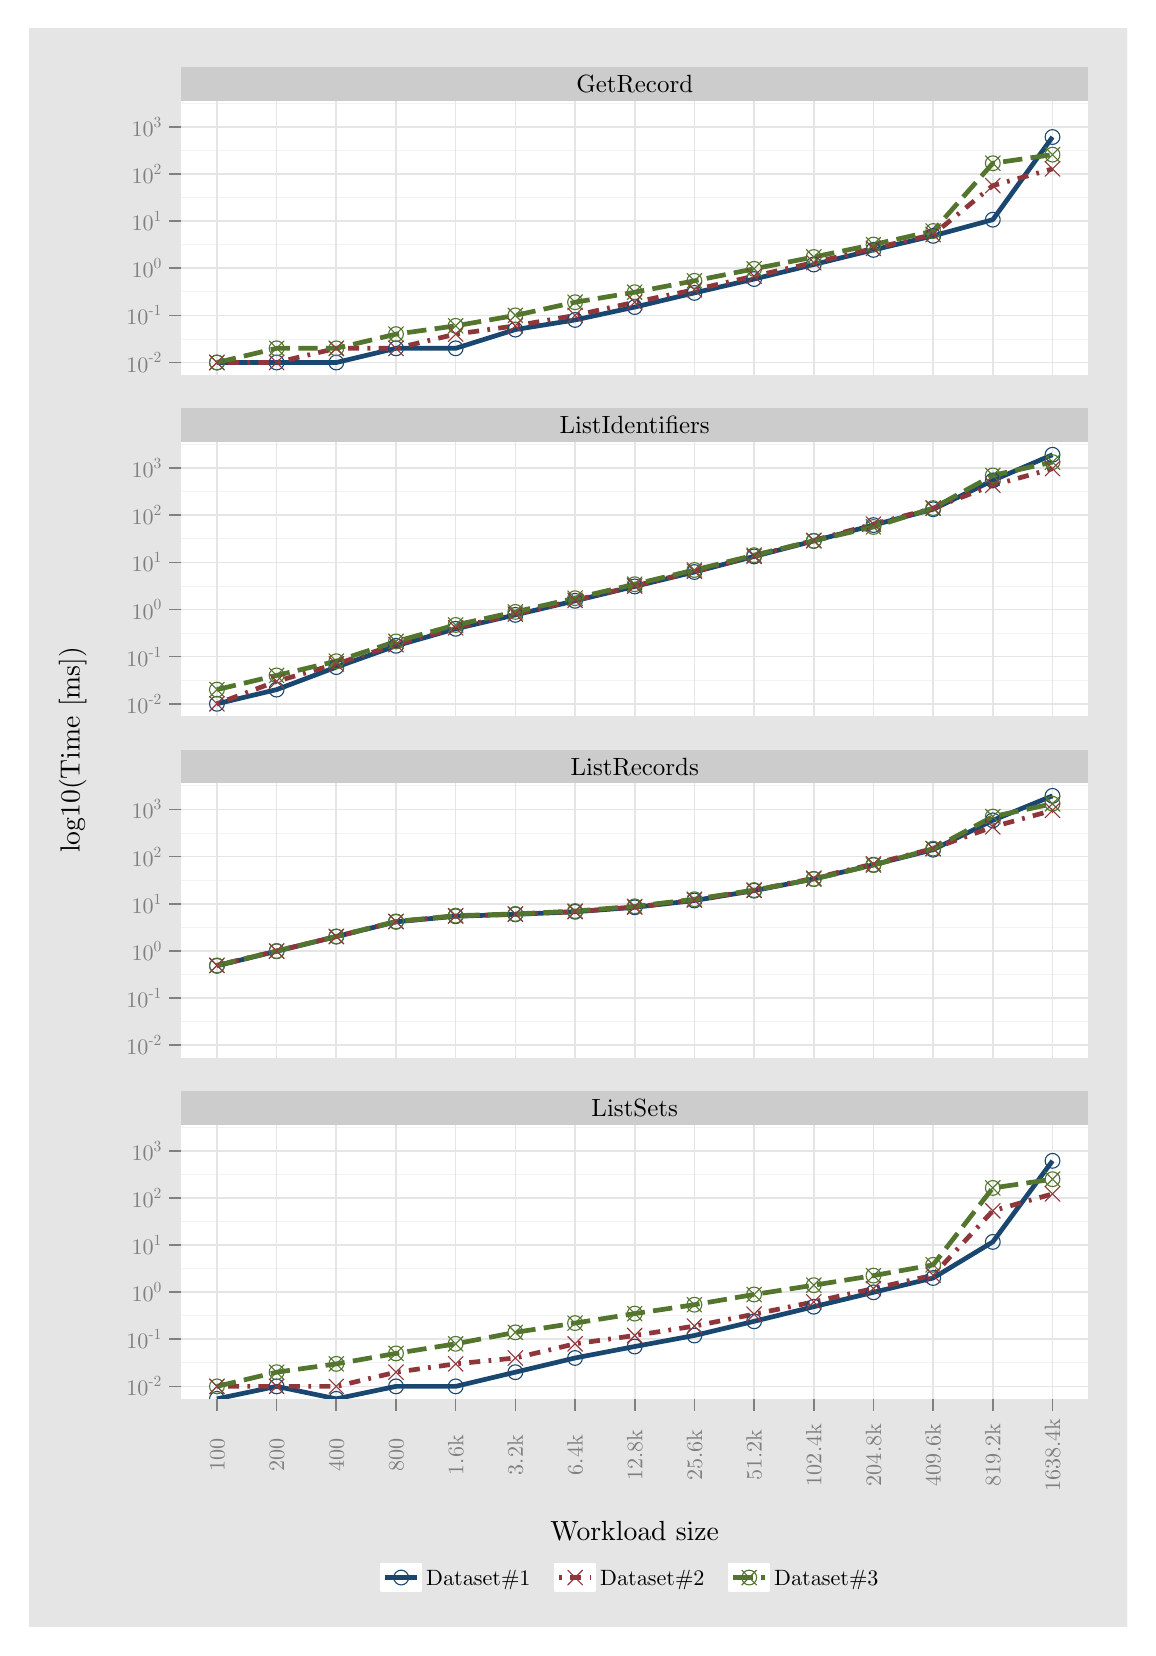
\begin{tikzpicture}[x=1pt,y=1pt]
\definecolor[named]{fillColor}{rgb}{1.00,1.00,1.00}
\path[use as bounding box,fill=fillColor,fill opacity=0.00] (0,0) rectangle (397.48,578.16);
\begin{scope}
\path[clip] (  0.00,  0.00) rectangle (397.48,578.16);
\definecolor[named]{drawColor}{rgb}{1.00,1.00,1.00}
\definecolor[named]{fillColor}{rgb}{0.90,0.90,0.90}

\path[draw=drawColor,line width= 0.6pt,line join=round,line cap=round,fill=fillColor] (  0.00, -0.00) rectangle (397.48,578.16);
\end{scope}
\begin{scope}
\path[clip] ( 55.45,452.66) rectangle (383.26,551.71);
\definecolor[named]{fillColor}{rgb}{1.00,1.00,1.00}

\path[fill=fillColor] ( 55.45,452.66) rectangle (383.26,551.71);
\definecolor[named]{drawColor}{rgb}{0.95,0.95,0.95}

\path[draw=drawColor,line width= 0.3pt,line join=round] ( 55.45,465.68) --
	(383.26,465.68);

\path[draw=drawColor,line width= 0.3pt,line join=round] ( 55.45,482.71) --
	(383.26,482.71);

\path[draw=drawColor,line width= 0.3pt,line join=round] ( 55.45,499.74) --
	(383.26,499.74);

\path[draw=drawColor,line width= 0.3pt,line join=round] ( 55.45,516.77) --
	(383.26,516.77);

\path[draw=drawColor,line width= 0.3pt,line join=round] ( 55.45,533.80) --
	(383.26,533.80);

\path[draw=drawColor,line width= 0.3pt,line join=round] ( 55.45,550.84) --
	(383.26,550.84);
\definecolor[named]{drawColor}{rgb}{0.90,0.90,0.90}

\path[draw=drawColor,line width= 0.6pt,line join=round] ( 55.45,457.16) --
	(383.26,457.16);

\path[draw=drawColor,line width= 0.6pt,line join=round] ( 55.45,474.19) --
	(383.26,474.19);

\path[draw=drawColor,line width= 0.6pt,line join=round] ( 55.45,491.22) --
	(383.26,491.22);

\path[draw=drawColor,line width= 0.6pt,line join=round] ( 55.45,508.26) --
	(383.26,508.26);

\path[draw=drawColor,line width= 0.6pt,line join=round] ( 55.45,525.29) --
	(383.26,525.29);

\path[draw=drawColor,line width= 0.6pt,line join=round] ( 55.45,542.32) --
	(383.26,542.32);

\path[draw=drawColor,line width= 0.6pt,line join=round] ( 68.39,452.66) --
	( 68.39,551.71);

\path[draw=drawColor,line width= 0.6pt,line join=round] ( 89.95,452.66) --
	( 89.95,551.71);

\path[draw=drawColor,line width= 0.6pt,line join=round] (111.52,452.66) --
	(111.52,551.71);

\path[draw=drawColor,line width= 0.6pt,line join=round] (133.09,452.66) --
	(133.09,551.71);

\path[draw=drawColor,line width= 0.6pt,line join=round] (154.65,452.66) --
	(154.65,551.71);

\path[draw=drawColor,line width= 0.6pt,line join=round] (176.22,452.66) --
	(176.22,551.71);

\path[draw=drawColor,line width= 0.6pt,line join=round] (197.79,452.66) --
	(197.79,551.71);

\path[draw=drawColor,line width= 0.6pt,line join=round] (219.35,452.66) --
	(219.35,551.71);

\path[draw=drawColor,line width= 0.6pt,line join=round] (240.92,452.66) --
	(240.92,551.71);

\path[draw=drawColor,line width= 0.6pt,line join=round] (262.49,452.66) --
	(262.49,551.71);

\path[draw=drawColor,line width= 0.6pt,line join=round] (284.05,452.66) --
	(284.05,551.71);

\path[draw=drawColor,line width= 0.6pt,line join=round] (305.62,452.66) --
	(305.62,551.71);

\path[draw=drawColor,line width= 0.6pt,line join=round] (327.19,452.66) --
	(327.19,551.71);

\path[draw=drawColor,line width= 0.6pt,line join=round] (348.75,452.66) --
	(348.75,551.71);

\path[draw=drawColor,line width= 0.6pt,line join=round] (370.32,452.66) --
	(370.32,551.71);
\definecolor[named]{drawColor}{rgb}{0.10,0.28,0.44}

\path[draw=drawColor,line width= 1.7pt,line join=round] ( 68.39,457.16) --
	( 89.95,457.16) --
	(111.52,457.16) --
	(133.09,462.29) --
	(154.65,462.29) --
	(176.22,469.06) --
	(197.79,472.54) --
	(219.35,477.19) --
	(240.92,482.32) --
	(262.49,487.32) --
	(284.05,492.57) --
	(305.62,497.85) --
	(327.19,502.93) --
	(348.75,508.77) --
	(370.32,538.64);
\definecolor[named]{drawColor}{rgb}{0.56,0.21,0.23}

\path[draw=drawColor,line width= 1.7pt,dash pattern=on 1pt off 3pt on 4pt off 3pt ,line join=round] ( 68.39,457.16) --
	( 89.95,457.16) --
	(111.52,462.29) --
	(133.09,462.29) --
	(154.65,467.41) --
	(176.22,470.41) --
	(197.79,474.19) --
	(219.35,478.94) --
	(240.92,483.46) --
	(262.49,488.37) --
	(284.05,493.28) --
	(305.62,498.38) --
	(327.19,503.42) --
	(348.75,521.08) --
	(370.32,527.11);
\definecolor[named]{drawColor}{rgb}{0.33,0.46,0.18}

\path[draw=drawColor,line width= 1.7pt,dash pattern=on 7pt off 3pt ,line join=round] ( 68.39,457.16) --
	( 89.95,462.29) --
	(111.52,462.29) --
	(133.09,467.41) --
	(154.65,470.41) --
	(176.22,474.19) --
	(197.79,478.94) --
	(219.35,482.56) --
	(240.92,486.67) --
	(262.49,491.00) --
	(284.05,495.28) --
	(305.62,499.78) --
	(327.19,504.67) --
	(348.75,529.16) --
	(370.32,532.27);
\definecolor[named]{drawColor}{rgb}{0.10,0.28,0.44}

\path[draw=drawColor,line width= 0.4pt,line join=round,line cap=round] ( 68.39,457.16) circle (  2.67);

\path[draw=drawColor,line width= 0.4pt,line join=round,line cap=round] ( 89.95,457.16) circle (  2.67);

\path[draw=drawColor,line width= 0.4pt,line join=round,line cap=round] (111.52,457.16) circle (  2.67);

\path[draw=drawColor,line width= 0.4pt,line join=round,line cap=round] (133.09,462.29) circle (  2.67);

\path[draw=drawColor,line width= 0.4pt,line join=round,line cap=round] (154.65,462.29) circle (  2.67);

\path[draw=drawColor,line width= 0.4pt,line join=round,line cap=round] (176.22,469.06) circle (  2.67);

\path[draw=drawColor,line width= 0.4pt,line join=round,line cap=round] (197.79,472.54) circle (  2.67);

\path[draw=drawColor,line width= 0.4pt,line join=round,line cap=round] (219.35,477.19) circle (  2.67);

\path[draw=drawColor,line width= 0.4pt,line join=round,line cap=round] (240.92,482.32) circle (  2.67);

\path[draw=drawColor,line width= 0.4pt,line join=round,line cap=round] (262.49,487.32) circle (  2.67);

\path[draw=drawColor,line width= 0.4pt,line join=round,line cap=round] (284.05,492.57) circle (  2.67);

\path[draw=drawColor,line width= 0.4pt,line join=round,line cap=round] (305.62,497.85) circle (  2.67);

\path[draw=drawColor,line width= 0.4pt,line join=round,line cap=round] (327.19,502.93) circle (  2.67);

\path[draw=drawColor,line width= 0.4pt,line join=round,line cap=round] (348.75,508.77) circle (  2.67);

\path[draw=drawColor,line width= 0.4pt,line join=round,line cap=round] (370.32,538.64) circle (  2.67);
\definecolor[named]{drawColor}{rgb}{0.33,0.46,0.18}

\path[draw=drawColor,line width= 0.4pt,line join=round,line cap=round] ( 68.39,457.16) circle (  2.67);

\path[draw=drawColor,line width= 0.4pt,line join=round,line cap=round] ( 65.72,454.49) -- ( 71.06,459.83);

\path[draw=drawColor,line width= 0.4pt,line join=round,line cap=round] ( 65.72,459.83) -- ( 71.06,454.49);

\path[draw=drawColor,line width= 0.4pt,line join=round,line cap=round] ( 89.95,462.29) circle (  2.67);

\path[draw=drawColor,line width= 0.4pt,line join=round,line cap=round] ( 87.29,459.62) -- ( 92.62,464.95);

\path[draw=drawColor,line width= 0.4pt,line join=round,line cap=round] ( 87.29,464.95) -- ( 92.62,459.62);

\path[draw=drawColor,line width= 0.4pt,line join=round,line cap=round] (111.52,462.29) circle (  2.67);

\path[draw=drawColor,line width= 0.4pt,line join=round,line cap=round] (108.85,459.62) -- (114.19,464.95);

\path[draw=drawColor,line width= 0.4pt,line join=round,line cap=round] (108.85,464.95) -- (114.19,459.62);

\path[draw=drawColor,line width= 0.4pt,line join=round,line cap=round] (133.09,467.41) circle (  2.67);

\path[draw=drawColor,line width= 0.4pt,line join=round,line cap=round] (130.42,464.75) -- (135.76,470.08);

\path[draw=drawColor,line width= 0.4pt,line join=round,line cap=round] (130.42,470.08) -- (135.76,464.75);

\path[draw=drawColor,line width= 0.4pt,line join=round,line cap=round] (154.65,470.41) circle (  2.67);

\path[draw=drawColor,line width= 0.4pt,line join=round,line cap=round] (151.99,467.75) -- (157.32,473.08);

\path[draw=drawColor,line width= 0.4pt,line join=round,line cap=round] (151.99,473.08) -- (157.32,467.75);

\path[draw=drawColor,line width= 0.4pt,line join=round,line cap=round] (176.22,474.19) circle (  2.67);

\path[draw=drawColor,line width= 0.4pt,line join=round,line cap=round] (173.55,471.52) -- (178.89,476.86);

\path[draw=drawColor,line width= 0.4pt,line join=round,line cap=round] (173.55,476.86) -- (178.89,471.52);

\path[draw=drawColor,line width= 0.4pt,line join=round,line cap=round] (197.79,478.94) circle (  2.67);

\path[draw=drawColor,line width= 0.4pt,line join=round,line cap=round] (195.12,476.27) -- (200.45,481.61);

\path[draw=drawColor,line width= 0.4pt,line join=round,line cap=round] (195.12,481.61) -- (200.45,476.27);

\path[draw=drawColor,line width= 0.4pt,line join=round,line cap=round] (219.35,482.56) circle (  2.67);

\path[draw=drawColor,line width= 0.4pt,line join=round,line cap=round] (216.69,479.89) -- (222.02,485.23);

\path[draw=drawColor,line width= 0.4pt,line join=round,line cap=round] (216.69,485.23) -- (222.02,479.89);

\path[draw=drawColor,line width= 0.4pt,line join=round,line cap=round] (240.92,486.67) circle (  2.67);

\path[draw=drawColor,line width= 0.4pt,line join=round,line cap=round] (238.25,484.00) -- (243.59,489.33);

\path[draw=drawColor,line width= 0.4pt,line join=round,line cap=round] (238.25,489.33) -- (243.59,484.00);

\path[draw=drawColor,line width= 0.4pt,line join=round,line cap=round] (262.49,491.00) circle (  2.67);

\path[draw=drawColor,line width= 0.4pt,line join=round,line cap=round] (259.82,488.33) -- (265.15,493.67);

\path[draw=drawColor,line width= 0.4pt,line join=round,line cap=round] (259.82,493.67) -- (265.15,488.33);

\path[draw=drawColor,line width= 0.4pt,line join=round,line cap=round] (284.05,495.28) circle (  2.67);

\path[draw=drawColor,line width= 0.4pt,line join=round,line cap=round] (281.39,492.61) -- (286.72,497.95);

\path[draw=drawColor,line width= 0.4pt,line join=round,line cap=round] (281.39,497.95) -- (286.72,492.61);

\path[draw=drawColor,line width= 0.4pt,line join=round,line cap=round] (305.62,499.78) circle (  2.67);

\path[draw=drawColor,line width= 0.4pt,line join=round,line cap=round] (302.95,497.11) -- (308.29,502.45);

\path[draw=drawColor,line width= 0.4pt,line join=round,line cap=round] (302.95,502.45) -- (308.29,497.11);

\path[draw=drawColor,line width= 0.4pt,line join=round,line cap=round] (327.19,504.67) circle (  2.67);

\path[draw=drawColor,line width= 0.4pt,line join=round,line cap=round] (324.52,502.00) -- (329.85,507.34);

\path[draw=drawColor,line width= 0.4pt,line join=round,line cap=round] (324.52,507.34) -- (329.85,502.00);

\path[draw=drawColor,line width= 0.4pt,line join=round,line cap=round] (348.75,529.16) circle (  2.67);

\path[draw=drawColor,line width= 0.4pt,line join=round,line cap=round] (346.08,526.50) -- (351.42,531.83);

\path[draw=drawColor,line width= 0.4pt,line join=round,line cap=round] (346.08,531.83) -- (351.42,526.50);

\path[draw=drawColor,line width= 0.4pt,line join=round,line cap=round] (370.32,532.27) circle (  2.67);

\path[draw=drawColor,line width= 0.4pt,line join=round,line cap=round] (367.65,529.61) -- (372.99,534.94);

\path[draw=drawColor,line width= 0.4pt,line join=round,line cap=round] (367.65,534.94) -- (372.99,529.61);
\definecolor[named]{drawColor}{rgb}{0.56,0.21,0.23}

\path[draw=drawColor,line width= 0.4pt,line join=round,line cap=round,fill=fillColor] ( 65.72,454.49) -- ( 71.06,459.83);

\path[draw=drawColor,line width= 0.4pt,line join=round,line cap=round,fill=fillColor] ( 65.72,459.83) -- ( 71.06,454.49);

\path[draw=drawColor,line width= 0.4pt,line join=round,line cap=round,fill=fillColor] ( 87.29,454.49) -- ( 92.62,459.83);

\path[draw=drawColor,line width= 0.4pt,line join=round,line cap=round,fill=fillColor] ( 87.29,459.83) -- ( 92.62,454.49);

\path[draw=drawColor,line width= 0.4pt,line join=round,line cap=round,fill=fillColor] (108.85,459.62) -- (114.19,464.95);

\path[draw=drawColor,line width= 0.4pt,line join=round,line cap=round,fill=fillColor] (108.85,464.95) -- (114.19,459.62);

\path[draw=drawColor,line width= 0.4pt,line join=round,line cap=round,fill=fillColor] (130.42,459.62) -- (135.76,464.95);

\path[draw=drawColor,line width= 0.4pt,line join=round,line cap=round,fill=fillColor] (130.42,464.95) -- (135.76,459.62);

\path[draw=drawColor,line width= 0.4pt,line join=round,line cap=round,fill=fillColor] (151.99,464.75) -- (157.32,470.08);

\path[draw=drawColor,line width= 0.4pt,line join=round,line cap=round,fill=fillColor] (151.99,470.08) -- (157.32,464.75);

\path[draw=drawColor,line width= 0.4pt,line join=round,line cap=round,fill=fillColor] (173.55,467.75) -- (178.89,473.08);

\path[draw=drawColor,line width= 0.4pt,line join=round,line cap=round,fill=fillColor] (173.55,473.08) -- (178.89,467.75);

\path[draw=drawColor,line width= 0.4pt,line join=round,line cap=round,fill=fillColor] (195.12,471.52) -- (200.45,476.86);

\path[draw=drawColor,line width= 0.4pt,line join=round,line cap=round,fill=fillColor] (195.12,476.86) -- (200.45,471.52);

\path[draw=drawColor,line width= 0.4pt,line join=round,line cap=round,fill=fillColor] (216.69,476.27) -- (222.02,481.61);

\path[draw=drawColor,line width= 0.4pt,line join=round,line cap=round,fill=fillColor] (216.69,481.61) -- (222.02,476.27);

\path[draw=drawColor,line width= 0.4pt,line join=round,line cap=round,fill=fillColor] (238.25,480.79) -- (243.59,486.13);

\path[draw=drawColor,line width= 0.4pt,line join=round,line cap=round,fill=fillColor] (238.25,486.13) -- (243.59,480.79);

\path[draw=drawColor,line width= 0.4pt,line join=round,line cap=round,fill=fillColor] (259.82,485.70) -- (265.15,491.04);

\path[draw=drawColor,line width= 0.4pt,line join=round,line cap=round,fill=fillColor] (259.82,491.04) -- (265.15,485.70);

\path[draw=drawColor,line width= 0.4pt,line join=round,line cap=round,fill=fillColor] (281.39,490.61) -- (286.72,495.94);

\path[draw=drawColor,line width= 0.4pt,line join=round,line cap=round,fill=fillColor] (281.39,495.94) -- (286.72,490.61);

\path[draw=drawColor,line width= 0.4pt,line join=round,line cap=round,fill=fillColor] (302.95,495.71) -- (308.29,501.04);

\path[draw=drawColor,line width= 0.4pt,line join=round,line cap=round,fill=fillColor] (302.95,501.04) -- (308.29,495.71);

\path[draw=drawColor,line width= 0.4pt,line join=round,line cap=round,fill=fillColor] (324.52,500.75) -- (329.85,506.09);

\path[draw=drawColor,line width= 0.4pt,line join=round,line cap=round,fill=fillColor] (324.52,506.09) -- (329.85,500.75);

\path[draw=drawColor,line width= 0.4pt,line join=round,line cap=round,fill=fillColor] (346.08,518.42) -- (351.42,523.75);

\path[draw=drawColor,line width= 0.4pt,line join=round,line cap=round,fill=fillColor] (346.08,523.75) -- (351.42,518.42);

\path[draw=drawColor,line width= 0.4pt,line join=round,line cap=round,fill=fillColor] (367.65,524.45) -- (372.99,529.78);

\path[draw=drawColor,line width= 0.4pt,line join=round,line cap=round,fill=fillColor] (367.65,529.78) -- (372.99,524.45);
\end{scope}
\begin{scope}
\path[clip] ( 55.45,329.33) rectangle (383.26,428.39);
\definecolor[named]{fillColor}{rgb}{1.00,1.00,1.00}

\path[fill=fillColor] ( 55.45,329.33) rectangle (383.26,428.39);
\definecolor[named]{drawColor}{rgb}{0.95,0.95,0.95}

\path[draw=drawColor,line width= 0.3pt,line join=round] ( 55.45,342.35) --
	(383.26,342.35);

\path[draw=drawColor,line width= 0.3pt,line join=round] ( 55.45,359.39) --
	(383.26,359.39);

\path[draw=drawColor,line width= 0.3pt,line join=round] ( 55.45,376.42) --
	(383.26,376.42);

\path[draw=drawColor,line width= 0.3pt,line join=round] ( 55.45,393.45) --
	(383.26,393.45);

\path[draw=drawColor,line width= 0.3pt,line join=round] ( 55.45,410.48) --
	(383.26,410.48);

\path[draw=drawColor,line width= 0.3pt,line join=round] ( 55.45,427.51) --
	(383.26,427.51);
\definecolor[named]{drawColor}{rgb}{0.90,0.90,0.90}

\path[draw=drawColor,line width= 0.6pt,line join=round] ( 55.45,333.84) --
	(383.26,333.84);

\path[draw=drawColor,line width= 0.6pt,line join=round] ( 55.45,350.87) --
	(383.26,350.87);

\path[draw=drawColor,line width= 0.6pt,line join=round] ( 55.45,367.90) --
	(383.26,367.90);

\path[draw=drawColor,line width= 0.6pt,line join=round] ( 55.45,384.93) --
	(383.26,384.93);

\path[draw=drawColor,line width= 0.6pt,line join=round] ( 55.45,401.97) --
	(383.26,401.97);

\path[draw=drawColor,line width= 0.6pt,line join=round] ( 55.45,419.00) --
	(383.26,419.00);

\path[draw=drawColor,line width= 0.6pt,line join=round] ( 68.39,329.33) --
	( 68.39,428.39);

\path[draw=drawColor,line width= 0.6pt,line join=round] ( 89.95,329.33) --
	( 89.95,428.39);

\path[draw=drawColor,line width= 0.6pt,line join=round] (111.52,329.33) --
	(111.52,428.39);

\path[draw=drawColor,line width= 0.6pt,line join=round] (133.09,329.33) --
	(133.09,428.39);

\path[draw=drawColor,line width= 0.6pt,line join=round] (154.65,329.33) --
	(154.65,428.39);

\path[draw=drawColor,line width= 0.6pt,line join=round] (176.22,329.33) --
	(176.22,428.39);

\path[draw=drawColor,line width= 0.6pt,line join=round] (197.79,329.33) --
	(197.79,428.39);

\path[draw=drawColor,line width= 0.6pt,line join=round] (219.35,329.33) --
	(219.35,428.39);

\path[draw=drawColor,line width= 0.6pt,line join=round] (240.92,329.33) --
	(240.92,428.39);

\path[draw=drawColor,line width= 0.6pt,line join=round] (262.49,329.33) --
	(262.49,428.39);

\path[draw=drawColor,line width= 0.6pt,line join=round] (284.05,329.33) --
	(284.05,428.39);

\path[draw=drawColor,line width= 0.6pt,line join=round] (305.62,329.33) --
	(305.62,428.39);

\path[draw=drawColor,line width= 0.6pt,line join=round] (327.19,329.33) --
	(327.19,428.39);

\path[draw=drawColor,line width= 0.6pt,line join=round] (348.75,329.33) --
	(348.75,428.39);

\path[draw=drawColor,line width= 0.6pt,line join=round] (370.32,329.33) --
	(370.32,428.39);
\definecolor[named]{drawColor}{rgb}{0.10,0.28,0.44}

\path[draw=drawColor,line width= 1.7pt,line join=round] ( 68.39,333.84) --
	( 89.95,338.96) --
	(111.52,347.09) --
	(133.09,354.79) --
	(154.65,360.94) --
	(176.22,365.97) --
	(197.79,371.05) --
	(219.35,376.25) --
	(240.92,381.46) --
	(262.49,387.09) --
	(284.05,392.67) --
	(305.62,398.41) --
	(327.19,404.13) --
	(348.75,414.55) --
	(370.32,423.83);
\definecolor[named]{drawColor}{rgb}{0.56,0.21,0.23}

\path[draw=drawColor,line width= 1.7pt,dash pattern=on 1pt off 3pt on 4pt off 3pt ,line join=round] ( 68.39,333.84) --
	( 89.95,341.96) --
	(111.52,348.23) --
	(133.09,355.22) --
	(154.65,361.31) --
	(176.22,366.25) --
	(197.79,371.24) --
	(219.35,376.41) --
	(240.92,381.71) --
	(262.49,387.13) --
	(284.05,392.90) --
	(305.62,398.77) --
	(327.19,404.53) --
	(348.75,412.80) --
	(370.32,418.80);
\definecolor[named]{drawColor}{rgb}{0.33,0.46,0.18}

\path[draw=drawColor,line width= 1.7pt,dash pattern=on 7pt off 3pt ,line join=round] ( 68.39,338.96) --
	( 89.95,344.09) --
	(111.52,349.22) --
	(133.09,356.36) --
	(154.65,362.32) --
	(176.22,367.04) --
	(197.79,372.00) --
	(219.35,377.04) --
	(240.92,382.19) --
	(262.49,387.54) --
	(284.05,392.75) --
	(305.62,397.74) --
	(327.19,404.56) --
	(348.75,416.36) --
	(370.32,421.17);
\definecolor[named]{drawColor}{rgb}{0.10,0.28,0.44}

\path[draw=drawColor,line width= 0.4pt,line join=round,line cap=round] ( 68.39,333.84) circle (  2.67);

\path[draw=drawColor,line width= 0.4pt,line join=round,line cap=round] ( 89.95,338.96) circle (  2.67);

\path[draw=drawColor,line width= 0.4pt,line join=round,line cap=round] (111.52,347.09) circle (  2.67);

\path[draw=drawColor,line width= 0.4pt,line join=round,line cap=round] (133.09,354.79) circle (  2.67);

\path[draw=drawColor,line width= 0.4pt,line join=round,line cap=round] (154.65,360.94) circle (  2.67);

\path[draw=drawColor,line width= 0.4pt,line join=round,line cap=round] (176.22,365.97) circle (  2.67);

\path[draw=drawColor,line width= 0.4pt,line join=round,line cap=round] (197.79,371.05) circle (  2.67);

\path[draw=drawColor,line width= 0.4pt,line join=round,line cap=round] (219.35,376.25) circle (  2.67);

\path[draw=drawColor,line width= 0.4pt,line join=round,line cap=round] (240.92,381.46) circle (  2.67);

\path[draw=drawColor,line width= 0.4pt,line join=round,line cap=round] (262.49,387.09) circle (  2.67);

\path[draw=drawColor,line width= 0.4pt,line join=round,line cap=round] (284.05,392.67) circle (  2.67);

\path[draw=drawColor,line width= 0.4pt,line join=round,line cap=round] (305.62,398.41) circle (  2.67);

\path[draw=drawColor,line width= 0.4pt,line join=round,line cap=round] (327.19,404.13) circle (  2.67);

\path[draw=drawColor,line width= 0.4pt,line join=round,line cap=round] (348.75,414.55) circle (  2.67);

\path[draw=drawColor,line width= 0.4pt,line join=round,line cap=round] (370.32,423.83) circle (  2.67);
\definecolor[named]{drawColor}{rgb}{0.33,0.46,0.18}

\path[draw=drawColor,line width= 0.4pt,line join=round,line cap=round] ( 68.39,338.96) circle (  2.67);

\path[draw=drawColor,line width= 0.4pt,line join=round,line cap=round] ( 65.72,336.30) -- ( 71.06,341.63);

\path[draw=drawColor,line width= 0.4pt,line join=round,line cap=round] ( 65.72,341.63) -- ( 71.06,336.30);

\path[draw=drawColor,line width= 0.4pt,line join=round,line cap=round] ( 89.95,344.09) circle (  2.67);

\path[draw=drawColor,line width= 0.4pt,line join=round,line cap=round] ( 87.29,341.42) -- ( 92.62,346.76);

\path[draw=drawColor,line width= 0.4pt,line join=round,line cap=round] ( 87.29,346.76) -- ( 92.62,341.42);

\path[draw=drawColor,line width= 0.4pt,line join=round,line cap=round] (111.52,349.22) circle (  2.67);

\path[draw=drawColor,line width= 0.4pt,line join=round,line cap=round] (108.85,346.55) -- (114.19,351.89);

\path[draw=drawColor,line width= 0.4pt,line join=round,line cap=round] (108.85,351.89) -- (114.19,346.55);

\path[draw=drawColor,line width= 0.4pt,line join=round,line cap=round] (133.09,356.36) circle (  2.67);

\path[draw=drawColor,line width= 0.4pt,line join=round,line cap=round] (130.42,353.69) -- (135.76,359.02);

\path[draw=drawColor,line width= 0.4pt,line join=round,line cap=round] (130.42,359.02) -- (135.76,353.69);

\path[draw=drawColor,line width= 0.4pt,line join=round,line cap=round] (154.65,362.32) circle (  2.67);

\path[draw=drawColor,line width= 0.4pt,line join=round,line cap=round] (151.99,359.65) -- (157.32,364.98);

\path[draw=drawColor,line width= 0.4pt,line join=round,line cap=round] (151.99,364.98) -- (157.32,359.65);

\path[draw=drawColor,line width= 0.4pt,line join=round,line cap=round] (176.22,367.04) circle (  2.67);

\path[draw=drawColor,line width= 0.4pt,line join=round,line cap=round] (173.55,364.37) -- (178.89,369.71);

\path[draw=drawColor,line width= 0.4pt,line join=round,line cap=round] (173.55,369.71) -- (178.89,364.37);

\path[draw=drawColor,line width= 0.4pt,line join=round,line cap=round] (197.79,372.00) circle (  2.67);

\path[draw=drawColor,line width= 0.4pt,line join=round,line cap=round] (195.12,369.33) -- (200.45,374.67);

\path[draw=drawColor,line width= 0.4pt,line join=round,line cap=round] (195.12,374.67) -- (200.45,369.33);

\path[draw=drawColor,line width= 0.4pt,line join=round,line cap=round] (219.35,377.04) circle (  2.67);

\path[draw=drawColor,line width= 0.4pt,line join=round,line cap=round] (216.69,374.37) -- (222.02,379.71);

\path[draw=drawColor,line width= 0.4pt,line join=round,line cap=round] (216.69,379.71) -- (222.02,374.37);

\path[draw=drawColor,line width= 0.4pt,line join=round,line cap=round] (240.92,382.19) circle (  2.67);

\path[draw=drawColor,line width= 0.4pt,line join=round,line cap=round] (238.25,379.52) -- (243.59,384.86);

\path[draw=drawColor,line width= 0.4pt,line join=round,line cap=round] (238.25,384.86) -- (243.59,379.52);

\path[draw=drawColor,line width= 0.4pt,line join=round,line cap=round] (262.49,387.54) circle (  2.67);

\path[draw=drawColor,line width= 0.4pt,line join=round,line cap=round] (259.82,384.88) -- (265.15,390.21);

\path[draw=drawColor,line width= 0.4pt,line join=round,line cap=round] (259.82,390.21) -- (265.15,384.88);

\path[draw=drawColor,line width= 0.4pt,line join=round,line cap=round] (284.05,392.75) circle (  2.67);

\path[draw=drawColor,line width= 0.4pt,line join=round,line cap=round] (281.39,390.08) -- (286.72,395.42);

\path[draw=drawColor,line width= 0.4pt,line join=round,line cap=round] (281.39,395.42) -- (286.72,390.08);

\path[draw=drawColor,line width= 0.4pt,line join=round,line cap=round] (305.62,397.74) circle (  2.67);

\path[draw=drawColor,line width= 0.4pt,line join=round,line cap=round] (302.95,395.08) -- (308.29,400.41);

\path[draw=drawColor,line width= 0.4pt,line join=round,line cap=round] (302.95,400.41) -- (308.29,395.08);

\path[draw=drawColor,line width= 0.4pt,line join=round,line cap=round] (327.19,404.56) circle (  2.67);

\path[draw=drawColor,line width= 0.4pt,line join=round,line cap=round] (324.52,401.89) -- (329.85,407.22);

\path[draw=drawColor,line width= 0.4pt,line join=round,line cap=round] (324.52,407.22) -- (329.85,401.89);

\path[draw=drawColor,line width= 0.4pt,line join=round,line cap=round] (348.75,416.36) circle (  2.67);

\path[draw=drawColor,line width= 0.4pt,line join=round,line cap=round] (346.08,413.69) -- (351.42,419.03);

\path[draw=drawColor,line width= 0.4pt,line join=round,line cap=round] (346.08,419.03) -- (351.42,413.69);

\path[draw=drawColor,line width= 0.4pt,line join=round,line cap=round] (370.32,421.17) circle (  2.67);

\path[draw=drawColor,line width= 0.4pt,line join=round,line cap=round] (367.65,418.51) -- (372.99,423.84);

\path[draw=drawColor,line width= 0.4pt,line join=round,line cap=round] (367.65,423.84) -- (372.99,418.51);
\definecolor[named]{drawColor}{rgb}{0.56,0.21,0.23}

\path[draw=drawColor,line width= 0.4pt,line join=round,line cap=round,fill=fillColor] ( 65.72,331.17) -- ( 71.06,336.50);

\path[draw=drawColor,line width= 0.4pt,line join=round,line cap=round,fill=fillColor] ( 65.72,336.50) -- ( 71.06,331.17);

\path[draw=drawColor,line width= 0.4pt,line join=round,line cap=round,fill=fillColor] ( 87.29,339.30) -- ( 92.62,344.63);

\path[draw=drawColor,line width= 0.4pt,line join=round,line cap=round,fill=fillColor] ( 87.29,344.63) -- ( 92.62,339.30);

\path[draw=drawColor,line width= 0.4pt,line join=round,line cap=round,fill=fillColor] (108.85,345.56) -- (114.19,350.90);

\path[draw=drawColor,line width= 0.4pt,line join=round,line cap=round,fill=fillColor] (108.85,350.90) -- (114.19,345.56);

\path[draw=drawColor,line width= 0.4pt,line join=round,line cap=round,fill=fillColor] (130.42,352.55) -- (135.76,357.88);

\path[draw=drawColor,line width= 0.4pt,line join=round,line cap=round,fill=fillColor] (130.42,357.88) -- (135.76,352.55);

\path[draw=drawColor,line width= 0.4pt,line join=round,line cap=round,fill=fillColor] (151.99,358.64) -- (157.32,363.97);

\path[draw=drawColor,line width= 0.4pt,line join=round,line cap=round,fill=fillColor] (151.99,363.97) -- (157.32,358.64);

\path[draw=drawColor,line width= 0.4pt,line join=round,line cap=round,fill=fillColor] (173.55,363.58) -- (178.89,368.92);

\path[draw=drawColor,line width= 0.4pt,line join=round,line cap=round,fill=fillColor] (173.55,368.92) -- (178.89,363.58);

\path[draw=drawColor,line width= 0.4pt,line join=round,line cap=round,fill=fillColor] (195.12,368.57) -- (200.45,373.91);

\path[draw=drawColor,line width= 0.4pt,line join=round,line cap=round,fill=fillColor] (195.12,373.91) -- (200.45,368.57);

\path[draw=drawColor,line width= 0.4pt,line join=round,line cap=round,fill=fillColor] (216.69,373.74) -- (222.02,379.08);

\path[draw=drawColor,line width= 0.4pt,line join=round,line cap=round,fill=fillColor] (216.69,379.08) -- (222.02,373.74);

\path[draw=drawColor,line width= 0.4pt,line join=round,line cap=round,fill=fillColor] (238.25,379.05) -- (243.59,384.38);

\path[draw=drawColor,line width= 0.4pt,line join=round,line cap=round,fill=fillColor] (238.25,384.38) -- (243.59,379.05);

\path[draw=drawColor,line width= 0.4pt,line join=round,line cap=round,fill=fillColor] (259.82,384.46) -- (265.15,389.79);

\path[draw=drawColor,line width= 0.4pt,line join=round,line cap=round,fill=fillColor] (259.82,389.79) -- (265.15,384.46);

\path[draw=drawColor,line width= 0.4pt,line join=round,line cap=round,fill=fillColor] (281.39,390.24) -- (286.72,395.57);

\path[draw=drawColor,line width= 0.4pt,line join=round,line cap=round,fill=fillColor] (281.39,395.57) -- (286.72,390.24);

\path[draw=drawColor,line width= 0.4pt,line join=round,line cap=round,fill=fillColor] (302.95,396.10) -- (308.29,401.44);

\path[draw=drawColor,line width= 0.4pt,line join=round,line cap=round,fill=fillColor] (302.95,401.44) -- (308.29,396.10);

\path[draw=drawColor,line width= 0.4pt,line join=round,line cap=round,fill=fillColor] (324.52,401.86) -- (329.85,407.20);

\path[draw=drawColor,line width= 0.4pt,line join=round,line cap=round,fill=fillColor] (324.52,407.20) -- (329.85,401.86);

\path[draw=drawColor,line width= 0.4pt,line join=round,line cap=round,fill=fillColor] (346.08,410.13) -- (351.42,415.47);

\path[draw=drawColor,line width= 0.4pt,line join=round,line cap=round,fill=fillColor] (346.08,415.47) -- (351.42,410.13);

\path[draw=drawColor,line width= 0.4pt,line join=round,line cap=round,fill=fillColor] (367.65,416.13) -- (372.99,421.47);

\path[draw=drawColor,line width= 0.4pt,line join=round,line cap=round,fill=fillColor] (367.65,421.47) -- (372.99,416.13);
\end{scope}
\begin{scope}
\path[clip] ( 55.45,206.01) rectangle (383.26,305.07);
\definecolor[named]{fillColor}{rgb}{1.00,1.00,1.00}

\path[fill=fillColor] ( 55.45,206.01) rectangle (383.26,305.07);
\definecolor[named]{drawColor}{rgb}{0.95,0.95,0.95}

\path[draw=drawColor,line width= 0.3pt,line join=round] ( 55.45,219.03) --
	(383.26,219.03);

\path[draw=drawColor,line width= 0.3pt,line join=round] ( 55.45,236.06) --
	(383.26,236.06);

\path[draw=drawColor,line width= 0.3pt,line join=round] ( 55.45,253.10) --
	(383.26,253.10);

\path[draw=drawColor,line width= 0.3pt,line join=round] ( 55.45,270.13) --
	(383.26,270.13);

\path[draw=drawColor,line width= 0.3pt,line join=round] ( 55.45,287.16) --
	(383.26,287.16);

\path[draw=drawColor,line width= 0.3pt,line join=round] ( 55.45,304.19) --
	(383.26,304.19);
\definecolor[named]{drawColor}{rgb}{0.90,0.90,0.90}

\path[draw=drawColor,line width= 0.6pt,line join=round] ( 55.45,210.52) --
	(383.26,210.52);

\path[draw=drawColor,line width= 0.6pt,line join=round] ( 55.45,227.55) --
	(383.26,227.55);

\path[draw=drawColor,line width= 0.6pt,line join=round] ( 55.45,244.58) --
	(383.26,244.58);

\path[draw=drawColor,line width= 0.6pt,line join=round] ( 55.45,261.61) --
	(383.26,261.61);

\path[draw=drawColor,line width= 0.6pt,line join=round] ( 55.45,278.64) --
	(383.26,278.64);

\path[draw=drawColor,line width= 0.6pt,line join=round] ( 55.45,295.68) --
	(383.26,295.68);

\path[draw=drawColor,line width= 0.6pt,line join=round] ( 68.39,206.01) --
	( 68.39,305.07);

\path[draw=drawColor,line width= 0.6pt,line join=round] ( 89.95,206.01) --
	( 89.95,305.07);

\path[draw=drawColor,line width= 0.6pt,line join=round] (111.52,206.01) --
	(111.52,305.07);

\path[draw=drawColor,line width= 0.6pt,line join=round] (133.09,206.01) --
	(133.09,305.07);

\path[draw=drawColor,line width= 0.6pt,line join=round] (154.65,206.01) --
	(154.65,305.07);

\path[draw=drawColor,line width= 0.6pt,line join=round] (176.22,206.01) --
	(176.22,305.07);

\path[draw=drawColor,line width= 0.6pt,line join=round] (197.79,206.01) --
	(197.79,305.07);

\path[draw=drawColor,line width= 0.6pt,line join=round] (219.35,206.01) --
	(219.35,305.07);

\path[draw=drawColor,line width= 0.6pt,line join=round] (240.92,206.01) --
	(240.92,305.07);

\path[draw=drawColor,line width= 0.6pt,line join=round] (262.49,206.01) --
	(262.49,305.07);

\path[draw=drawColor,line width= 0.6pt,line join=round] (284.05,206.01) --
	(284.05,305.07);

\path[draw=drawColor,line width= 0.6pt,line join=round] (305.62,206.01) --
	(305.62,305.07);

\path[draw=drawColor,line width= 0.6pt,line join=round] (327.19,206.01) --
	(327.19,305.07);

\path[draw=drawColor,line width= 0.6pt,line join=round] (348.75,206.01) --
	(348.75,305.07);

\path[draw=drawColor,line width= 0.6pt,line join=round] (370.32,206.01) --
	(370.32,305.07);
\definecolor[named]{drawColor}{rgb}{0.10,0.28,0.44}

\path[draw=drawColor,line width= 1.7pt,line join=round] ( 68.39,239.15) --
	( 89.95,244.43) --
	(111.52,249.71) --
	(133.09,255.05) --
	(154.65,257.07) --
	(176.22,257.76) --
	(197.79,258.68) --
	(219.35,260.30) --
	(240.92,262.76) --
	(262.49,266.32) --
	(284.05,270.55) --
	(305.62,275.68) --
	(327.19,281.12) --
	(348.75,291.73) --
	(370.32,300.57);
\definecolor[named]{drawColor}{rgb}{0.56,0.21,0.23}

\path[draw=drawColor,line width= 1.7pt,dash pattern=on 1pt off 3pt on 4pt off 3pt ,line join=round] ( 68.39,239.30) --
	( 89.95,244.51) --
	(111.52,249.74) --
	(133.09,255.14) --
	(154.65,257.15) --
	(176.22,257.80) --
	(197.79,258.74) --
	(219.35,260.40) --
	(240.92,262.94) --
	(262.49,266.40) --
	(284.05,270.80) --
	(305.62,275.99) --
	(327.19,281.53) --
	(348.75,289.36) --
	(370.32,295.31);
\definecolor[named]{drawColor}{rgb}{0.33,0.46,0.18}

\path[draw=drawColor,line width= 1.7pt,dash pattern=on 7pt off 3pt ,line join=round] ( 68.39,239.30) --
	( 89.95,244.51) --
	(111.52,249.78) --
	(133.09,255.19) --
	(154.65,257.28) --
	(176.22,257.91) --
	(197.79,258.95) --
	(219.35,260.66) --
	(240.92,263.22) --
	(262.49,266.52) --
	(284.05,270.51) --
	(305.62,275.55) --
	(327.19,281.50) --
	(348.75,293.08) --
	(370.32,297.72);
\definecolor[named]{drawColor}{rgb}{0.10,0.28,0.44}

\path[draw=drawColor,line width= 0.4pt,line join=round,line cap=round] ( 68.39,239.15) circle (  2.67);

\path[draw=drawColor,line width= 0.4pt,line join=round,line cap=round] ( 89.95,244.43) circle (  2.67);

\path[draw=drawColor,line width= 0.4pt,line join=round,line cap=round] (111.52,249.71) circle (  2.67);

\path[draw=drawColor,line width= 0.4pt,line join=round,line cap=round] (133.09,255.05) circle (  2.67);

\path[draw=drawColor,line width= 0.4pt,line join=round,line cap=round] (154.65,257.07) circle (  2.67);

\path[draw=drawColor,line width= 0.4pt,line join=round,line cap=round] (176.22,257.76) circle (  2.67);

\path[draw=drawColor,line width= 0.4pt,line join=round,line cap=round] (197.79,258.68) circle (  2.67);

\path[draw=drawColor,line width= 0.4pt,line join=round,line cap=round] (219.35,260.30) circle (  2.67);

\path[draw=drawColor,line width= 0.4pt,line join=round,line cap=round] (240.92,262.76) circle (  2.67);

\path[draw=drawColor,line width= 0.4pt,line join=round,line cap=round] (262.49,266.32) circle (  2.67);

\path[draw=drawColor,line width= 0.4pt,line join=round,line cap=round] (284.05,270.55) circle (  2.67);

\path[draw=drawColor,line width= 0.4pt,line join=round,line cap=round] (305.62,275.68) circle (  2.67);

\path[draw=drawColor,line width= 0.4pt,line join=round,line cap=round] (327.19,281.12) circle (  2.67);

\path[draw=drawColor,line width= 0.4pt,line join=round,line cap=round] (348.75,291.73) circle (  2.67);

\path[draw=drawColor,line width= 0.4pt,line join=round,line cap=round] (370.32,300.57) circle (  2.67);
\definecolor[named]{drawColor}{rgb}{0.33,0.46,0.18}

\path[draw=drawColor,line width= 0.4pt,line join=round,line cap=round] ( 68.39,239.30) circle (  2.67);

\path[draw=drawColor,line width= 0.4pt,line join=round,line cap=round] ( 65.72,236.64) -- ( 71.06,241.97);

\path[draw=drawColor,line width= 0.4pt,line join=round,line cap=round] ( 65.72,241.97) -- ( 71.06,236.64);

\path[draw=drawColor,line width= 0.4pt,line join=round,line cap=round] ( 89.95,244.51) circle (  2.67);

\path[draw=drawColor,line width= 0.4pt,line join=round,line cap=round] ( 87.29,241.84) -- ( 92.62,247.17);

\path[draw=drawColor,line width= 0.4pt,line join=round,line cap=round] ( 87.29,247.17) -- ( 92.62,241.84);

\path[draw=drawColor,line width= 0.4pt,line join=round,line cap=round] (111.52,249.78) circle (  2.67);

\path[draw=drawColor,line width= 0.4pt,line join=round,line cap=round] (108.85,247.11) -- (114.19,252.45);

\path[draw=drawColor,line width= 0.4pt,line join=round,line cap=round] (108.85,252.45) -- (114.19,247.11);

\path[draw=drawColor,line width= 0.4pt,line join=round,line cap=round] (133.09,255.19) circle (  2.67);

\path[draw=drawColor,line width= 0.4pt,line join=round,line cap=round] (130.42,252.53) -- (135.76,257.86);

\path[draw=drawColor,line width= 0.4pt,line join=round,line cap=round] (130.42,257.86) -- (135.76,252.53);

\path[draw=drawColor,line width= 0.4pt,line join=round,line cap=round] (154.65,257.28) circle (  2.67);

\path[draw=drawColor,line width= 0.4pt,line join=round,line cap=round] (151.99,254.62) -- (157.32,259.95);

\path[draw=drawColor,line width= 0.4pt,line join=round,line cap=round] (151.99,259.95) -- (157.32,254.62);

\path[draw=drawColor,line width= 0.4pt,line join=round,line cap=round] (176.22,257.91) circle (  2.67);

\path[draw=drawColor,line width= 0.4pt,line join=round,line cap=round] (173.55,255.24) -- (178.89,260.57);

\path[draw=drawColor,line width= 0.4pt,line join=round,line cap=round] (173.55,260.57) -- (178.89,255.24);

\path[draw=drawColor,line width= 0.4pt,line join=round,line cap=round] (197.79,258.95) circle (  2.67);

\path[draw=drawColor,line width= 0.4pt,line join=round,line cap=round] (195.12,256.28) -- (200.45,261.62);

\path[draw=drawColor,line width= 0.4pt,line join=round,line cap=round] (195.12,261.62) -- (200.45,256.28);

\path[draw=drawColor,line width= 0.4pt,line join=round,line cap=round] (219.35,260.66) circle (  2.67);

\path[draw=drawColor,line width= 0.4pt,line join=round,line cap=round] (216.69,257.99) -- (222.02,263.32);

\path[draw=drawColor,line width= 0.4pt,line join=round,line cap=round] (216.69,263.32) -- (222.02,257.99);

\path[draw=drawColor,line width= 0.4pt,line join=round,line cap=round] (240.92,263.22) circle (  2.67);

\path[draw=drawColor,line width= 0.4pt,line join=round,line cap=round] (238.25,260.55) -- (243.59,265.89);

\path[draw=drawColor,line width= 0.4pt,line join=round,line cap=round] (238.25,265.89) -- (243.59,260.55);

\path[draw=drawColor,line width= 0.4pt,line join=round,line cap=round] (262.49,266.52) circle (  2.67);

\path[draw=drawColor,line width= 0.4pt,line join=round,line cap=round] (259.82,263.86) -- (265.15,269.19);

\path[draw=drawColor,line width= 0.4pt,line join=round,line cap=round] (259.82,269.19) -- (265.15,263.86);

\path[draw=drawColor,line width= 0.4pt,line join=round,line cap=round] (284.05,270.51) circle (  2.67);

\path[draw=drawColor,line width= 0.4pt,line join=round,line cap=round] (281.39,267.84) -- (286.72,273.18);

\path[draw=drawColor,line width= 0.4pt,line join=round,line cap=round] (281.39,273.18) -- (286.72,267.84);

\path[draw=drawColor,line width= 0.4pt,line join=round,line cap=round] (305.62,275.55) circle (  2.67);

\path[draw=drawColor,line width= 0.4pt,line join=round,line cap=round] (302.95,272.88) -- (308.29,278.21);

\path[draw=drawColor,line width= 0.4pt,line join=round,line cap=round] (302.95,278.21) -- (308.29,272.88);

\path[draw=drawColor,line width= 0.4pt,line join=round,line cap=round] (327.19,281.50) circle (  2.67);

\path[draw=drawColor,line width= 0.4pt,line join=round,line cap=round] (324.52,278.84) -- (329.85,284.17);

\path[draw=drawColor,line width= 0.4pt,line join=round,line cap=round] (324.52,284.17) -- (329.85,278.84);

\path[draw=drawColor,line width= 0.4pt,line join=round,line cap=round] (348.75,293.08) circle (  2.67);

\path[draw=drawColor,line width= 0.4pt,line join=round,line cap=round] (346.08,290.41) -- (351.42,295.75);

\path[draw=drawColor,line width= 0.4pt,line join=round,line cap=round] (346.08,295.75) -- (351.42,290.41);

\path[draw=drawColor,line width= 0.4pt,line join=round,line cap=round] (370.32,297.72) circle (  2.67);

\path[draw=drawColor,line width= 0.4pt,line join=round,line cap=round] (367.65,295.05) -- (372.99,300.38);

\path[draw=drawColor,line width= 0.4pt,line join=round,line cap=round] (367.65,300.38) -- (372.99,295.05);
\definecolor[named]{drawColor}{rgb}{0.56,0.21,0.23}

\path[draw=drawColor,line width= 0.4pt,line join=round,line cap=round,fill=fillColor] ( 65.72,236.64) -- ( 71.06,241.97);

\path[draw=drawColor,line width= 0.4pt,line join=round,line cap=round,fill=fillColor] ( 65.72,241.97) -- ( 71.06,236.64);

\path[draw=drawColor,line width= 0.4pt,line join=round,line cap=round,fill=fillColor] ( 87.29,241.84) -- ( 92.62,247.17);

\path[draw=drawColor,line width= 0.4pt,line join=round,line cap=round,fill=fillColor] ( 87.29,247.17) -- ( 92.62,241.84);

\path[draw=drawColor,line width= 0.4pt,line join=round,line cap=round,fill=fillColor] (108.85,247.08) -- (114.19,252.41);

\path[draw=drawColor,line width= 0.4pt,line join=round,line cap=round,fill=fillColor] (108.85,252.41) -- (114.19,247.08);

\path[draw=drawColor,line width= 0.4pt,line join=round,line cap=round,fill=fillColor] (130.42,252.47) -- (135.76,257.81);

\path[draw=drawColor,line width= 0.4pt,line join=round,line cap=round,fill=fillColor] (130.42,257.81) -- (135.76,252.47);

\path[draw=drawColor,line width= 0.4pt,line join=round,line cap=round,fill=fillColor] (151.99,254.48) -- (157.32,259.82);

\path[draw=drawColor,line width= 0.4pt,line join=round,line cap=round,fill=fillColor] (151.99,259.82) -- (157.32,254.48);

\path[draw=drawColor,line width= 0.4pt,line join=round,line cap=round,fill=fillColor] (173.55,255.13) -- (178.89,260.46);

\path[draw=drawColor,line width= 0.4pt,line join=round,line cap=round,fill=fillColor] (173.55,260.46) -- (178.89,255.13);

\path[draw=drawColor,line width= 0.4pt,line join=round,line cap=round,fill=fillColor] (195.12,256.07) -- (200.45,261.40);

\path[draw=drawColor,line width= 0.4pt,line join=round,line cap=round,fill=fillColor] (195.12,261.40) -- (200.45,256.07);

\path[draw=drawColor,line width= 0.4pt,line join=round,line cap=round,fill=fillColor] (216.69,257.73) -- (222.02,263.07);

\path[draw=drawColor,line width= 0.4pt,line join=round,line cap=round,fill=fillColor] (216.69,263.07) -- (222.02,257.73);

\path[draw=drawColor,line width= 0.4pt,line join=round,line cap=round,fill=fillColor] (238.25,260.27) -- (243.59,265.61);

\path[draw=drawColor,line width= 0.4pt,line join=round,line cap=round,fill=fillColor] (238.25,265.61) -- (243.59,260.27);

\path[draw=drawColor,line width= 0.4pt,line join=round,line cap=round,fill=fillColor] (259.82,263.73) -- (265.15,269.07);

\path[draw=drawColor,line width= 0.4pt,line join=round,line cap=round,fill=fillColor] (259.82,269.07) -- (265.15,263.73);

\path[draw=drawColor,line width= 0.4pt,line join=round,line cap=round,fill=fillColor] (281.39,268.13) -- (286.72,273.47);

\path[draw=drawColor,line width= 0.4pt,line join=round,line cap=round,fill=fillColor] (281.39,273.47) -- (286.72,268.13);

\path[draw=drawColor,line width= 0.4pt,line join=round,line cap=round,fill=fillColor] (302.95,273.32) -- (308.29,278.65);

\path[draw=drawColor,line width= 0.4pt,line join=round,line cap=round,fill=fillColor] (302.95,278.65) -- (308.29,273.32);

\path[draw=drawColor,line width= 0.4pt,line join=round,line cap=round,fill=fillColor] (324.52,278.87) -- (329.85,284.20);

\path[draw=drawColor,line width= 0.4pt,line join=round,line cap=round,fill=fillColor] (324.52,284.20) -- (329.85,278.87);

\path[draw=drawColor,line width= 0.4pt,line join=round,line cap=round,fill=fillColor] (346.08,286.69) -- (351.42,292.02);

\path[draw=drawColor,line width= 0.4pt,line join=round,line cap=round,fill=fillColor] (346.08,292.02) -- (351.42,286.69);

\path[draw=drawColor,line width= 0.4pt,line join=round,line cap=round,fill=fillColor] (367.65,292.64) -- (372.99,297.98);

\path[draw=drawColor,line width= 0.4pt,line join=round,line cap=round,fill=fillColor] (367.65,297.98) -- (372.99,292.64);
\end{scope}
\begin{scope}
\path[clip] ( 55.45, 82.69) rectangle (383.26,181.75);
\definecolor[named]{fillColor}{rgb}{1.00,1.00,1.00}

\path[fill=fillColor] ( 55.45, 82.69) rectangle (383.26,181.75);
\definecolor[named]{drawColor}{rgb}{0.95,0.95,0.95}

\path[draw=drawColor,line width= 0.3pt,line join=round] ( 55.45, 95.71) --
	(383.26, 95.71);

\path[draw=drawColor,line width= 0.3pt,line join=round] ( 55.45,112.74) --
	(383.26,112.74);

\path[draw=drawColor,line width= 0.3pt,line join=round] ( 55.45,129.77) --
	(383.26,129.77);

\path[draw=drawColor,line width= 0.3pt,line join=round] ( 55.45,146.81) --
	(383.26,146.81);

\path[draw=drawColor,line width= 0.3pt,line join=round] ( 55.45,163.84) --
	(383.26,163.84);

\path[draw=drawColor,line width= 0.3pt,line join=round] ( 55.45,180.87) --
	(383.26,180.87);
\definecolor[named]{drawColor}{rgb}{0.90,0.90,0.90}

\path[draw=drawColor,line width= 0.6pt,line join=round] ( 55.45, 87.19) --
	(383.26, 87.19);

\path[draw=drawColor,line width= 0.6pt,line join=round] ( 55.45,104.23) --
	(383.26,104.23);

\path[draw=drawColor,line width= 0.6pt,line join=round] ( 55.45,121.26) --
	(383.26,121.26);

\path[draw=drawColor,line width= 0.6pt,line join=round] ( 55.45,138.29) --
	(383.26,138.29);

\path[draw=drawColor,line width= 0.6pt,line join=round] ( 55.45,155.32) --
	(383.26,155.32);

\path[draw=drawColor,line width= 0.6pt,line join=round] ( 55.45,172.35) --
	(383.26,172.35);

\path[draw=drawColor,line width= 0.6pt,line join=round] ( 68.39, 82.69) --
	( 68.39,181.75);

\path[draw=drawColor,line width= 0.6pt,line join=round] ( 89.95, 82.69) --
	( 89.95,181.75);

\path[draw=drawColor,line width= 0.6pt,line join=round] (111.52, 82.69) --
	(111.52,181.75);

\path[draw=drawColor,line width= 0.6pt,line join=round] (133.09, 82.69) --
	(133.09,181.75);

\path[draw=drawColor,line width= 0.6pt,line join=round] (154.65, 82.69) --
	(154.65,181.75);

\path[draw=drawColor,line width= 0.6pt,line join=round] (176.22, 82.69) --
	(176.22,181.75);

\path[draw=drawColor,line width= 0.6pt,line join=round] (197.79, 82.69) --
	(197.79,181.75);

\path[draw=drawColor,line width= 0.6pt,line join=round] (219.35, 82.69) --
	(219.35,181.75);

\path[draw=drawColor,line width= 0.6pt,line join=round] (240.92, 82.69) --
	(240.92,181.75);

\path[draw=drawColor,line width= 0.6pt,line join=round] (262.49, 82.69) --
	(262.49,181.75);

\path[draw=drawColor,line width= 0.6pt,line join=round] (284.05, 82.69) --
	(284.05,181.75);

\path[draw=drawColor,line width= 0.6pt,line join=round] (305.62, 82.69) --
	(305.62,181.75);

\path[draw=drawColor,line width= 0.6pt,line join=round] (327.19, 82.69) --
	(327.19,181.75);

\path[draw=drawColor,line width= 0.6pt,line join=round] (348.75, 82.69) --
	(348.75,181.75);

\path[draw=drawColor,line width= 0.6pt,line join=round] (370.32, 82.69) --
	(370.32,181.75);
\definecolor[named]{drawColor}{rgb}{0.10,0.28,0.44}

\path[draw=drawColor,line width= 1.7pt,line join=round] ( 68.39, 82.69) --
	( 89.95, 87.19) --
	(111.52, 82.69) --
	(133.09, 87.19) --
	(154.65, 87.19) --
	(176.22, 92.32) --
	(197.79, 97.45) --
	(219.35,101.59) --
	(240.92,105.57) --
	(262.49,110.70) --
	(284.05,115.98) --
	(305.62,121.18) --
	(327.19,126.35) --
	(348.75,139.39) --
	(370.32,168.69);
\definecolor[named]{drawColor}{rgb}{0.56,0.21,0.23}

\path[draw=drawColor,line width= 1.7pt,dash pattern=on 1pt off 3pt on 4pt off 3pt ,line join=round] ( 68.39, 87.19) --
	( 89.95, 87.19) --
	(111.52, 87.19) --
	(133.09, 92.32) --
	(154.65, 95.32) --
	(176.22, 97.45) --
	(197.79,102.57) --
	(219.35,105.57) --
	(240.92,108.97) --
	(262.49,113.28) --
	(284.05,117.72) --
	(305.62,122.54) --
	(327.19,127.35) --
	(348.75,150.64) --
	(370.32,156.73);
\definecolor[named]{drawColor}{rgb}{0.33,0.46,0.18}

\path[draw=drawColor,line width= 1.7pt,dash pattern=on 7pt off 3pt ,line join=round] ( 68.39, 87.19) --
	( 89.95, 92.32) --
	(111.52, 95.32) --
	(133.09, 99.10) --
	(154.65,102.57) --
	(176.22,106.71) --
	(197.79,110.06) --
	(219.35,113.49) --
	(240.92,116.70) --
	(262.49,120.40) --
	(284.05,123.75) --
	(305.62,127.22) --
	(327.19,131.11) --
	(348.75,158.89) --
	(370.32,162.05);
\definecolor[named]{drawColor}{rgb}{0.10,0.28,0.44}

\path[draw=drawColor,line width= 0.4pt,line join=round,line cap=round] ( 68.39, 82.69) circle (  2.67);

\path[draw=drawColor,line width= 0.4pt,line join=round,line cap=round] ( 89.95, 87.19) circle (  2.67);

\path[draw=drawColor,line width= 0.4pt,line join=round,line cap=round] (111.52, 82.69) circle (  2.67);

\path[draw=drawColor,line width= 0.4pt,line join=round,line cap=round] (133.09, 87.19) circle (  2.67);

\path[draw=drawColor,line width= 0.4pt,line join=round,line cap=round] (154.65, 87.19) circle (  2.67);

\path[draw=drawColor,line width= 0.4pt,line join=round,line cap=round] (176.22, 92.32) circle (  2.67);

\path[draw=drawColor,line width= 0.4pt,line join=round,line cap=round] (197.79, 97.45) circle (  2.67);

\path[draw=drawColor,line width= 0.4pt,line join=round,line cap=round] (219.35,101.59) circle (  2.67);

\path[draw=drawColor,line width= 0.4pt,line join=round,line cap=round] (240.92,105.57) circle (  2.67);

\path[draw=drawColor,line width= 0.4pt,line join=round,line cap=round] (262.49,110.70) circle (  2.67);

\path[draw=drawColor,line width= 0.4pt,line join=round,line cap=round] (284.05,115.98) circle (  2.67);

\path[draw=drawColor,line width= 0.4pt,line join=round,line cap=round] (305.62,121.18) circle (  2.67);

\path[draw=drawColor,line width= 0.4pt,line join=round,line cap=round] (327.19,126.35) circle (  2.67);

\path[draw=drawColor,line width= 0.4pt,line join=round,line cap=round] (348.75,139.39) circle (  2.67);

\path[draw=drawColor,line width= 0.4pt,line join=round,line cap=round] (370.32,168.69) circle (  2.67);
\definecolor[named]{drawColor}{rgb}{0.33,0.46,0.18}

\path[draw=drawColor,line width= 0.4pt,line join=round,line cap=round] ( 68.39, 87.19) circle (  2.67);

\path[draw=drawColor,line width= 0.4pt,line join=round,line cap=round] ( 65.72, 84.53) -- ( 71.06, 89.86);

\path[draw=drawColor,line width= 0.4pt,line join=round,line cap=round] ( 65.72, 89.86) -- ( 71.06, 84.53);

\path[draw=drawColor,line width= 0.4pt,line join=round,line cap=round] ( 89.95, 92.32) circle (  2.67);

\path[draw=drawColor,line width= 0.4pt,line join=round,line cap=round] ( 87.29, 89.65) -- ( 92.62, 94.99);

\path[draw=drawColor,line width= 0.4pt,line join=round,line cap=round] ( 87.29, 94.99) -- ( 92.62, 89.65);

\path[draw=drawColor,line width= 0.4pt,line join=round,line cap=round] (111.52, 95.32) circle (  2.67);

\path[draw=drawColor,line width= 0.4pt,line join=round,line cap=round] (108.85, 92.65) -- (114.19, 97.99);

\path[draw=drawColor,line width= 0.4pt,line join=round,line cap=round] (108.85, 97.99) -- (114.19, 92.65);

\path[draw=drawColor,line width= 0.4pt,line join=round,line cap=round] (133.09, 99.10) circle (  2.67);

\path[draw=drawColor,line width= 0.4pt,line join=round,line cap=round] (130.42, 96.43) -- (135.76,101.77);

\path[draw=drawColor,line width= 0.4pt,line join=round,line cap=round] (130.42,101.77) -- (135.76, 96.43);

\path[draw=drawColor,line width= 0.4pt,line join=round,line cap=round] (154.65,102.57) circle (  2.67);

\path[draw=drawColor,line width= 0.4pt,line join=round,line cap=round] (151.99, 99.91) -- (157.32,105.24);

\path[draw=drawColor,line width= 0.4pt,line join=round,line cap=round] (151.99,105.24) -- (157.32, 99.91);

\path[draw=drawColor,line width= 0.4pt,line join=round,line cap=round] (176.22,106.71) circle (  2.67);

\path[draw=drawColor,line width= 0.4pt,line join=round,line cap=round] (173.55,104.05) -- (178.89,109.38);

\path[draw=drawColor,line width= 0.4pt,line join=round,line cap=round] (173.55,109.38) -- (178.89,104.05);

\path[draw=drawColor,line width= 0.4pt,line join=round,line cap=round] (197.79,110.06) circle (  2.67);

\path[draw=drawColor,line width= 0.4pt,line join=round,line cap=round] (195.12,107.39) -- (200.45,112.72);

\path[draw=drawColor,line width= 0.4pt,line join=round,line cap=round] (195.12,112.72) -- (200.45,107.39);

\path[draw=drawColor,line width= 0.4pt,line join=round,line cap=round] (219.35,113.49) circle (  2.67);

\path[draw=drawColor,line width= 0.4pt,line join=round,line cap=round] (216.69,110.82) -- (222.02,116.16);

\path[draw=drawColor,line width= 0.4pt,line join=round,line cap=round] (216.69,116.16) -- (222.02,110.82);

\path[draw=drawColor,line width= 0.4pt,line join=round,line cap=round] (240.92,116.70) circle (  2.67);

\path[draw=drawColor,line width= 0.4pt,line join=round,line cap=round] (238.25,114.03) -- (243.59,119.37);

\path[draw=drawColor,line width= 0.4pt,line join=round,line cap=round] (238.25,119.37) -- (243.59,114.03);

\path[draw=drawColor,line width= 0.4pt,line join=round,line cap=round] (262.49,120.40) circle (  2.67);

\path[draw=drawColor,line width= 0.4pt,line join=round,line cap=round] (259.82,117.73) -- (265.15,123.06);

\path[draw=drawColor,line width= 0.4pt,line join=round,line cap=round] (259.82,123.06) -- (265.15,117.73);

\path[draw=drawColor,line width= 0.4pt,line join=round,line cap=round] (284.05,123.75) circle (  2.67);

\path[draw=drawColor,line width= 0.4pt,line join=round,line cap=round] (281.39,121.08) -- (286.72,126.41);

\path[draw=drawColor,line width= 0.4pt,line join=round,line cap=round] (281.39,126.41) -- (286.72,121.08);

\path[draw=drawColor,line width= 0.4pt,line join=round,line cap=round] (305.62,127.22) circle (  2.67);

\path[draw=drawColor,line width= 0.4pt,line join=round,line cap=round] (302.95,124.56) -- (308.29,129.89);

\path[draw=drawColor,line width= 0.4pt,line join=round,line cap=round] (302.95,129.89) -- (308.29,124.56);

\path[draw=drawColor,line width= 0.4pt,line join=round,line cap=round] (327.19,131.11) circle (  2.67);

\path[draw=drawColor,line width= 0.4pt,line join=round,line cap=round] (324.52,128.45) -- (329.85,133.78);

\path[draw=drawColor,line width= 0.4pt,line join=round,line cap=round] (324.52,133.78) -- (329.85,128.45);

\path[draw=drawColor,line width= 0.4pt,line join=round,line cap=round] (348.75,158.89) circle (  2.67);

\path[draw=drawColor,line width= 0.4pt,line join=round,line cap=round] (346.08,156.22) -- (351.42,161.56);

\path[draw=drawColor,line width= 0.4pt,line join=round,line cap=round] (346.08,161.56) -- (351.42,156.22);

\path[draw=drawColor,line width= 0.4pt,line join=round,line cap=round] (370.32,162.05) circle (  2.67);

\path[draw=drawColor,line width= 0.4pt,line join=round,line cap=round] (367.65,159.38) -- (372.99,164.71);

\path[draw=drawColor,line width= 0.4pt,line join=round,line cap=round] (367.65,164.71) -- (372.99,159.38);
\definecolor[named]{drawColor}{rgb}{0.56,0.21,0.23}

\path[draw=drawColor,line width= 0.4pt,line join=round,line cap=round,fill=fillColor] ( 65.72, 84.53) -- ( 71.06, 89.86);

\path[draw=drawColor,line width= 0.4pt,line join=round,line cap=round,fill=fillColor] ( 65.72, 89.86) -- ( 71.06, 84.53);

\path[draw=drawColor,line width= 0.4pt,line join=round,line cap=round,fill=fillColor] ( 87.29, 84.53) -- ( 92.62, 89.86);

\path[draw=drawColor,line width= 0.4pt,line join=round,line cap=round,fill=fillColor] ( 87.29, 89.86) -- ( 92.62, 84.53);

\path[draw=drawColor,line width= 0.4pt,line join=round,line cap=round,fill=fillColor] (108.85, 84.53) -- (114.19, 89.86);

\path[draw=drawColor,line width= 0.4pt,line join=round,line cap=round,fill=fillColor] (108.85, 89.86) -- (114.19, 84.53);

\path[draw=drawColor,line width= 0.4pt,line join=round,line cap=round,fill=fillColor] (130.42, 89.65) -- (135.76, 94.99);

\path[draw=drawColor,line width= 0.4pt,line join=round,line cap=round,fill=fillColor] (130.42, 94.99) -- (135.76, 89.65);

\path[draw=drawColor,line width= 0.4pt,line join=round,line cap=round,fill=fillColor] (151.99, 92.65) -- (157.32, 97.99);

\path[draw=drawColor,line width= 0.4pt,line join=round,line cap=round,fill=fillColor] (151.99, 97.99) -- (157.32, 92.65);

\path[draw=drawColor,line width= 0.4pt,line join=round,line cap=round,fill=fillColor] (173.55, 94.78) -- (178.89,100.12);

\path[draw=drawColor,line width= 0.4pt,line join=round,line cap=round,fill=fillColor] (173.55,100.12) -- (178.89, 94.78);

\path[draw=drawColor,line width= 0.4pt,line join=round,line cap=round,fill=fillColor] (195.12, 99.91) -- (200.45,105.24);

\path[draw=drawColor,line width= 0.4pt,line join=round,line cap=round,fill=fillColor] (195.12,105.24) -- (200.45, 99.91);

\path[draw=drawColor,line width= 0.4pt,line join=round,line cap=round,fill=fillColor] (216.69,102.91) -- (222.02,108.24);

\path[draw=drawColor,line width= 0.4pt,line join=round,line cap=round,fill=fillColor] (216.69,108.24) -- (222.02,102.91);

\path[draw=drawColor,line width= 0.4pt,line join=round,line cap=round,fill=fillColor] (238.25,106.31) -- (243.59,111.64);

\path[draw=drawColor,line width= 0.4pt,line join=round,line cap=round,fill=fillColor] (238.25,111.64) -- (243.59,106.31);

\path[draw=drawColor,line width= 0.4pt,line join=round,line cap=round,fill=fillColor] (259.82,110.61) -- (265.15,115.95);

\path[draw=drawColor,line width= 0.4pt,line join=round,line cap=round,fill=fillColor] (259.82,115.95) -- (265.15,110.61);

\path[draw=drawColor,line width= 0.4pt,line join=round,line cap=round,fill=fillColor] (281.39,115.05) -- (286.72,120.39);

\path[draw=drawColor,line width= 0.4pt,line join=round,line cap=round,fill=fillColor] (281.39,120.39) -- (286.72,115.05);

\path[draw=drawColor,line width= 0.4pt,line join=round,line cap=round,fill=fillColor] (302.95,119.88) -- (308.29,125.21);

\path[draw=drawColor,line width= 0.4pt,line join=round,line cap=round,fill=fillColor] (302.95,125.21) -- (308.29,119.88);

\path[draw=drawColor,line width= 0.4pt,line join=round,line cap=round,fill=fillColor] (324.52,124.69) -- (329.85,130.02);

\path[draw=drawColor,line width= 0.4pt,line join=round,line cap=round,fill=fillColor] (324.52,130.02) -- (329.85,124.69);

\path[draw=drawColor,line width= 0.4pt,line join=round,line cap=round,fill=fillColor] (346.08,147.97) -- (351.42,153.31);

\path[draw=drawColor,line width= 0.4pt,line join=round,line cap=round,fill=fillColor] (346.08,153.31) -- (351.42,147.97);

\path[draw=drawColor,line width= 0.4pt,line join=round,line cap=round,fill=fillColor] (367.65,154.07) -- (372.99,159.40);

\path[draw=drawColor,line width= 0.4pt,line join=round,line cap=round,fill=fillColor] (367.65,159.40) -- (372.99,154.07);
\end{scope}
\begin{scope}
\path[clip] (  0.00,  0.00) rectangle (397.48,578.16);
\definecolor[named]{fillColor}{rgb}{0.80,0.80,0.80}

\path[fill=fillColor] ( 55.45,551.71) rectangle (383.26,563.93);
\definecolor[named]{drawColor}{rgb}{0.00,0.00,0.00}

\node[text=drawColor,anchor=base,inner sep=0pt, outer sep=0pt, scale=  0.90] at (219.35,554.72) {GetRecord};
\end{scope}
\begin{scope}
\path[clip] (  0.00,  0.00) rectangle (397.48,578.16);
\definecolor[named]{fillColor}{rgb}{0.80,0.80,0.80}

\path[fill=fillColor] ( 55.45,428.39) rectangle (383.26,440.61);
\definecolor[named]{drawColor}{rgb}{0.00,0.00,0.00}

\node[text=drawColor,anchor=base,inner sep=0pt, outer sep=0pt, scale=  0.90] at (219.35,431.40) {ListIdentifiers};
\end{scope}
\begin{scope}
\path[clip] (  0.00,  0.00) rectangle (397.48,578.16);
\definecolor[named]{fillColor}{rgb}{0.80,0.80,0.80}

\path[fill=fillColor] ( 55.45,305.07) rectangle (383.26,317.29);
\definecolor[named]{drawColor}{rgb}{0.00,0.00,0.00}

\node[text=drawColor,anchor=base,inner sep=0pt, outer sep=0pt, scale=  0.90] at (219.35,308.08) {ListRecords};
\end{scope}
\begin{scope}
\path[clip] (  0.00,  0.00) rectangle (397.48,578.16);
\definecolor[named]{fillColor}{rgb}{0.80,0.80,0.80}

\path[fill=fillColor] ( 55.45,181.75) rectangle (383.26,193.97);
\definecolor[named]{drawColor}{rgb}{0.00,0.00,0.00}

\node[text=drawColor,anchor=base,inner sep=0pt, outer sep=0pt, scale=  0.90] at (219.35,184.76) {ListSets};
\end{scope}
\begin{scope}
\path[clip] (  0.00,  0.00) rectangle (397.48,578.16);
\definecolor[named]{drawColor}{rgb}{0.50,0.50,0.50}

\node[text=drawColor,anchor=base west,inner sep=0pt, outer sep=0pt, scale=  0.80] at ( 35.67,453.73) {10};

\node[text=drawColor,anchor=base west,inner sep=0pt, outer sep=0pt, scale=  0.56] at ( 43.67,457.00) {-};

\node[text=drawColor,anchor=base west,inner sep=0pt, outer sep=0pt, scale=  0.56] at ( 45.54,457.00) {2};

\node[text=drawColor,anchor=base west,inner sep=0pt, outer sep=0pt, scale=  0.80] at ( 35.67,470.76) {10};

\node[text=drawColor,anchor=base west,inner sep=0pt, outer sep=0pt, scale=  0.56] at ( 43.67,474.03) {-};

\node[text=drawColor,anchor=base west,inner sep=0pt, outer sep=0pt, scale=  0.56] at ( 45.54,474.03) {1};

\node[text=drawColor,anchor=base west,inner sep=0pt, outer sep=0pt, scale=  0.80] at ( 37.54,487.79) {10};

\node[text=drawColor,anchor=base west,inner sep=0pt, outer sep=0pt, scale=  0.56] at ( 45.54,491.06) {0};

\node[text=drawColor,anchor=base west,inner sep=0pt, outer sep=0pt, scale=  0.80] at ( 37.54,504.82) {10};

\node[text=drawColor,anchor=base west,inner sep=0pt, outer sep=0pt, scale=  0.56] at ( 45.54,508.09) {1};

\node[text=drawColor,anchor=base west,inner sep=0pt, outer sep=0pt, scale=  0.80] at ( 37.54,521.86) {10};

\node[text=drawColor,anchor=base west,inner sep=0pt, outer sep=0pt, scale=  0.56] at ( 45.54,525.13) {2};

\node[text=drawColor,anchor=base west,inner sep=0pt, outer sep=0pt, scale=  0.80] at ( 37.54,538.89) {10};

\node[text=drawColor,anchor=base west,inner sep=0pt, outer sep=0pt, scale=  0.56] at ( 45.54,542.16) {3};
\end{scope}
\begin{scope}
\path[clip] (  0.00,  0.00) rectangle (397.48,578.16);
\definecolor[named]{drawColor}{rgb}{0.50,0.50,0.50}

\path[draw=drawColor,line width= 0.6pt,line join=round] ( 51.18,457.16) --
	( 55.45,457.16);

\path[draw=drawColor,line width= 0.6pt,line join=round] ( 51.18,474.19) --
	( 55.45,474.19);

\path[draw=drawColor,line width= 0.6pt,line join=round] ( 51.18,491.22) --
	( 55.45,491.22);

\path[draw=drawColor,line width= 0.6pt,line join=round] ( 51.18,508.26) --
	( 55.45,508.26);

\path[draw=drawColor,line width= 0.6pt,line join=round] ( 51.18,525.29) --
	( 55.45,525.29);

\path[draw=drawColor,line width= 0.6pt,line join=round] ( 51.18,542.32) --
	( 55.45,542.32);
\end{scope}
\begin{scope}
\path[clip] (  0.00,  0.00) rectangle (397.48,578.16);
\definecolor[named]{drawColor}{rgb}{0.50,0.50,0.50}

\node[text=drawColor,anchor=base west,inner sep=0pt, outer sep=0pt, scale=  0.80] at ( 35.67,330.41) {10};

\node[text=drawColor,anchor=base west,inner sep=0pt, outer sep=0pt, scale=  0.56] at ( 43.67,333.68) {-};

\node[text=drawColor,anchor=base west,inner sep=0pt, outer sep=0pt, scale=  0.56] at ( 45.54,333.68) {2};

\node[text=drawColor,anchor=base west,inner sep=0pt, outer sep=0pt, scale=  0.80] at ( 35.67,347.44) {10};

\node[text=drawColor,anchor=base west,inner sep=0pt, outer sep=0pt, scale=  0.56] at ( 43.67,350.71) {-};

\node[text=drawColor,anchor=base west,inner sep=0pt, outer sep=0pt, scale=  0.56] at ( 45.54,350.71) {1};

\node[text=drawColor,anchor=base west,inner sep=0pt, outer sep=0pt, scale=  0.80] at ( 37.54,364.47) {10};

\node[text=drawColor,anchor=base west,inner sep=0pt, outer sep=0pt, scale=  0.56] at ( 45.54,367.74) {0};

\node[text=drawColor,anchor=base west,inner sep=0pt, outer sep=0pt, scale=  0.80] at ( 37.54,381.50) {10};

\node[text=drawColor,anchor=base west,inner sep=0pt, outer sep=0pt, scale=  0.56] at ( 45.54,384.77) {1};

\node[text=drawColor,anchor=base west,inner sep=0pt, outer sep=0pt, scale=  0.80] at ( 37.54,398.53) {10};

\node[text=drawColor,anchor=base west,inner sep=0pt, outer sep=0pt, scale=  0.56] at ( 45.54,401.80) {2};

\node[text=drawColor,anchor=base west,inner sep=0pt, outer sep=0pt, scale=  0.80] at ( 37.54,415.57) {10};

\node[text=drawColor,anchor=base west,inner sep=0pt, outer sep=0pt, scale=  0.56] at ( 45.54,418.84) {3};
\end{scope}
\begin{scope}
\path[clip] (  0.00,  0.00) rectangle (397.48,578.16);
\definecolor[named]{drawColor}{rgb}{0.50,0.50,0.50}

\path[draw=drawColor,line width= 0.6pt,line join=round] ( 51.18,333.84) --
	( 55.45,333.84);

\path[draw=drawColor,line width= 0.6pt,line join=round] ( 51.18,350.87) --
	( 55.45,350.87);

\path[draw=drawColor,line width= 0.6pt,line join=round] ( 51.18,367.90) --
	( 55.45,367.90);

\path[draw=drawColor,line width= 0.6pt,line join=round] ( 51.18,384.93) --
	( 55.45,384.93);

\path[draw=drawColor,line width= 0.6pt,line join=round] ( 51.18,401.97) --
	( 55.45,401.97);

\path[draw=drawColor,line width= 0.6pt,line join=round] ( 51.18,419.00) --
	( 55.45,419.00);
\end{scope}
\begin{scope}
\path[clip] (  0.00,  0.00) rectangle (397.48,578.16);
\definecolor[named]{drawColor}{rgb}{0.50,0.50,0.50}

\node[text=drawColor,anchor=base west,inner sep=0pt, outer sep=0pt, scale=  0.80] at ( 35.67,207.08) {10};

\node[text=drawColor,anchor=base west,inner sep=0pt, outer sep=0pt, scale=  0.56] at ( 43.67,210.35) {-};

\node[text=drawColor,anchor=base west,inner sep=0pt, outer sep=0pt, scale=  0.56] at ( 45.54,210.35) {2};

\node[text=drawColor,anchor=base west,inner sep=0pt, outer sep=0pt, scale=  0.80] at ( 35.67,224.12) {10};

\node[text=drawColor,anchor=base west,inner sep=0pt, outer sep=0pt, scale=  0.56] at ( 43.67,227.39) {-};

\node[text=drawColor,anchor=base west,inner sep=0pt, outer sep=0pt, scale=  0.56] at ( 45.54,227.39) {1};

\node[text=drawColor,anchor=base west,inner sep=0pt, outer sep=0pt, scale=  0.80] at ( 37.54,241.15) {10};

\node[text=drawColor,anchor=base west,inner sep=0pt, outer sep=0pt, scale=  0.56] at ( 45.54,244.42) {0};

\node[text=drawColor,anchor=base west,inner sep=0pt, outer sep=0pt, scale=  0.80] at ( 37.54,258.18) {10};

\node[text=drawColor,anchor=base west,inner sep=0pt, outer sep=0pt, scale=  0.56] at ( 45.54,261.45) {1};

\node[text=drawColor,anchor=base west,inner sep=0pt, outer sep=0pt, scale=  0.80] at ( 37.54,275.21) {10};

\node[text=drawColor,anchor=base west,inner sep=0pt, outer sep=0pt, scale=  0.56] at ( 45.54,278.48) {2};

\node[text=drawColor,anchor=base west,inner sep=0pt, outer sep=0pt, scale=  0.80] at ( 37.54,292.24) {10};

\node[text=drawColor,anchor=base west,inner sep=0pt, outer sep=0pt, scale=  0.56] at ( 45.54,295.51) {3};
\end{scope}
\begin{scope}
\path[clip] (  0.00,  0.00) rectangle (397.48,578.16);
\definecolor[named]{drawColor}{rgb}{0.50,0.50,0.50}

\path[draw=drawColor,line width= 0.6pt,line join=round] ( 51.18,210.52) --
	( 55.45,210.52);

\path[draw=drawColor,line width= 0.6pt,line join=round] ( 51.18,227.55) --
	( 55.45,227.55);

\path[draw=drawColor,line width= 0.6pt,line join=round] ( 51.18,244.58) --
	( 55.45,244.58);

\path[draw=drawColor,line width= 0.6pt,line join=round] ( 51.18,261.61) --
	( 55.45,261.61);

\path[draw=drawColor,line width= 0.6pt,line join=round] ( 51.18,278.64) --
	( 55.45,278.64);

\path[draw=drawColor,line width= 0.6pt,line join=round] ( 51.18,295.68) --
	( 55.45,295.68);
\end{scope}
\begin{scope}
\path[clip] (  0.00,  0.00) rectangle (397.48,578.16);
\definecolor[named]{drawColor}{rgb}{0.50,0.50,0.50}

\node[text=drawColor,anchor=base west,inner sep=0pt, outer sep=0pt, scale=  0.80] at ( 35.67, 83.76) {10};

\node[text=drawColor,anchor=base west,inner sep=0pt, outer sep=0pt, scale=  0.56] at ( 43.67, 87.03) {-};

\node[text=drawColor,anchor=base west,inner sep=0pt, outer sep=0pt, scale=  0.56] at ( 45.54, 87.03) {2};

\node[text=drawColor,anchor=base west,inner sep=0pt, outer sep=0pt, scale=  0.80] at ( 35.67,100.79) {10};

\node[text=drawColor,anchor=base west,inner sep=0pt, outer sep=0pt, scale=  0.56] at ( 43.67,104.06) {-};

\node[text=drawColor,anchor=base west,inner sep=0pt, outer sep=0pt, scale=  0.56] at ( 45.54,104.06) {1};

\node[text=drawColor,anchor=base west,inner sep=0pt, outer sep=0pt, scale=  0.80] at ( 37.54,117.83) {10};

\node[text=drawColor,anchor=base west,inner sep=0pt, outer sep=0pt, scale=  0.56] at ( 45.54,121.10) {0};

\node[text=drawColor,anchor=base west,inner sep=0pt, outer sep=0pt, scale=  0.80] at ( 37.54,134.86) {10};

\node[text=drawColor,anchor=base west,inner sep=0pt, outer sep=0pt, scale=  0.56] at ( 45.54,138.13) {1};

\node[text=drawColor,anchor=base west,inner sep=0pt, outer sep=0pt, scale=  0.80] at ( 37.54,151.89) {10};

\node[text=drawColor,anchor=base west,inner sep=0pt, outer sep=0pt, scale=  0.56] at ( 45.54,155.16) {2};

\node[text=drawColor,anchor=base west,inner sep=0pt, outer sep=0pt, scale=  0.80] at ( 37.54,168.92) {10};

\node[text=drawColor,anchor=base west,inner sep=0pt, outer sep=0pt, scale=  0.56] at ( 45.54,172.19) {3};
\end{scope}
\begin{scope}
\path[clip] (  0.00,  0.00) rectangle (397.48,578.16);
\definecolor[named]{drawColor}{rgb}{0.50,0.50,0.50}

\path[draw=drawColor,line width= 0.6pt,line join=round] ( 51.18, 87.19) --
	( 55.45, 87.19);

\path[draw=drawColor,line width= 0.6pt,line join=round] ( 51.18,104.23) --
	( 55.45,104.23);

\path[draw=drawColor,line width= 0.6pt,line join=round] ( 51.18,121.26) --
	( 55.45,121.26);

\path[draw=drawColor,line width= 0.6pt,line join=round] ( 51.18,138.29) --
	( 55.45,138.29);

\path[draw=drawColor,line width= 0.6pt,line join=round] ( 51.18,155.32) --
	( 55.45,155.32);

\path[draw=drawColor,line width= 0.6pt,line join=round] ( 51.18,172.35) --
	( 55.45,172.35);
\end{scope}
\begin{scope}
\path[clip] (  0.00,  0.00) rectangle (397.48,578.16);
\definecolor[named]{drawColor}{rgb}{0.50,0.50,0.50}

\path[draw=drawColor,line width= 0.6pt,line join=round] ( 68.39, 78.42) --
	( 68.39, 82.69);

\path[draw=drawColor,line width= 0.6pt,line join=round] ( 89.95, 78.42) --
	( 89.95, 82.69);

\path[draw=drawColor,line width= 0.6pt,line join=round] (111.52, 78.42) --
	(111.52, 82.69);

\path[draw=drawColor,line width= 0.6pt,line join=round] (133.09, 78.42) --
	(133.09, 82.69);

\path[draw=drawColor,line width= 0.6pt,line join=round] (154.65, 78.42) --
	(154.65, 82.69);

\path[draw=drawColor,line width= 0.6pt,line join=round] (176.22, 78.42) --
	(176.22, 82.69);

\path[draw=drawColor,line width= 0.6pt,line join=round] (197.79, 78.42) --
	(197.79, 82.69);

\path[draw=drawColor,line width= 0.6pt,line join=round] (219.35, 78.42) --
	(219.35, 82.69);

\path[draw=drawColor,line width= 0.6pt,line join=round] (240.92, 78.42) --
	(240.92, 82.69);

\path[draw=drawColor,line width= 0.6pt,line join=round] (262.49, 78.42) --
	(262.49, 82.69);

\path[draw=drawColor,line width= 0.6pt,line join=round] (284.05, 78.42) --
	(284.05, 82.69);

\path[draw=drawColor,line width= 0.6pt,line join=round] (305.62, 78.42) --
	(305.62, 82.69);

\path[draw=drawColor,line width= 0.6pt,line join=round] (327.19, 78.42) --
	(327.19, 82.69);

\path[draw=drawColor,line width= 0.6pt,line join=round] (348.75, 78.42) --
	(348.75, 82.69);

\path[draw=drawColor,line width= 0.6pt,line join=round] (370.32, 78.42) --
	(370.32, 82.69);
\end{scope}
\begin{scope}
\path[clip] (  0.00,  0.00) rectangle (397.48,578.16);
\definecolor[named]{drawColor}{rgb}{0.50,0.50,0.50}

\node[text=drawColor,rotate= 90.00,anchor=base,inner sep=0pt, outer sep=0pt, scale=  0.80] at ( 71.14, 62.36) {100};

\node[text=drawColor,rotate= 90.00,anchor=base,inner sep=0pt, outer sep=0pt, scale=  0.80] at ( 92.71, 62.36) {200};

\node[text=drawColor,rotate= 90.00,anchor=base,inner sep=0pt, outer sep=0pt, scale=  0.80] at (114.28, 62.36) {400};

\node[text=drawColor,rotate= 90.00,anchor=base,inner sep=0pt, outer sep=0pt, scale=  0.80] at (135.84, 62.36) {800};

\node[text=drawColor,rotate= 90.00,anchor=base,inner sep=0pt, outer sep=0pt, scale=  0.80] at (157.41, 62.36) {1.6k};

\node[text=drawColor,rotate= 90.00,anchor=base,inner sep=0pt, outer sep=0pt, scale=  0.80] at (178.98, 62.36) {3.2k};

\node[text=drawColor,rotate= 90.00,anchor=base,inner sep=0pt, outer sep=0pt, scale=  0.80] at (200.54, 62.36) {6.4k};

\node[text=drawColor,rotate= 90.00,anchor=base,inner sep=0pt, outer sep=0pt, scale=  0.80] at (222.11, 62.36) {12.8k};

\node[text=drawColor,rotate= 90.00,anchor=base,inner sep=0pt, outer sep=0pt, scale=  0.80] at (243.67, 62.36) {25.6k};

\node[text=drawColor,rotate= 90.00,anchor=base,inner sep=0pt, outer sep=0pt, scale=  0.80] at (265.24, 62.36) {51.2k};

\node[text=drawColor,rotate= 90.00,anchor=base,inner sep=0pt, outer sep=0pt, scale=  0.80] at (286.81, 62.36) {102.4k};

\node[text=drawColor,rotate= 90.00,anchor=base,inner sep=0pt, outer sep=0pt, scale=  0.80] at (308.37, 62.36) {204.8k};

\node[text=drawColor,rotate= 90.00,anchor=base,inner sep=0pt, outer sep=0pt, scale=  0.80] at (329.94, 62.36) {409.6k};

\node[text=drawColor,rotate= 90.00,anchor=base,inner sep=0pt, outer sep=0pt, scale=  0.80] at (351.51, 62.36) {819.2k};

\node[text=drawColor,rotate= 90.00,anchor=base,inner sep=0pt, outer sep=0pt, scale=  0.80] at (373.07, 62.36) {1638.4k};
\end{scope}
\begin{scope}
\path[clip] (  0.00,  0.00) rectangle (397.48,578.16);
\definecolor[named]{drawColor}{rgb}{0.00,0.00,0.00}

\node[text=drawColor,anchor=base,inner sep=0pt, outer sep=0pt, scale=  1.00] at (219.35, 31.41) {Workload size};
\end{scope}
\begin{scope}
\path[clip] (  0.00,  0.00) rectangle (397.48,578.16);
\definecolor[named]{drawColor}{rgb}{0.00,0.00,0.00}

\node[text=drawColor,rotate= 90.00,anchor=base,inner sep=0pt, outer sep=0pt, scale=  1.00] at ( 18.80,317.20) {log10(Time [ms])};
\end{scope}
\begin{scope}
\path[clip] (  0.00,  0.00) rectangle (397.48,578.16);
\definecolor[named]{fillColor}{rgb}{0.90,0.90,0.90}

\path[fill=fillColor] (119.86,  8.87) rectangle (318.84, 27.36);
\end{scope}
\begin{scope}
\path[clip] (  0.00,  0.00) rectangle (397.48,578.16);
\definecolor[named]{drawColor}{rgb}{1.00,1.00,1.00}
\definecolor[named]{fillColor}{rgb}{1.00,1.00,1.00}

\path[draw=drawColor,line width= 0.6pt,line join=round,line cap=round,fill=fillColor] (127.74, 13.14) rectangle (142.20, 23.09);
\end{scope}
\begin{scope}
\path[clip] (  0.00,  0.00) rectangle (397.48,578.16);
\definecolor[named]{drawColor}{rgb}{0.10,0.28,0.44}

\path[draw=drawColor,line width= 1.7pt,line join=round] (129.19, 18.11) -- (140.75, 18.11);
\end{scope}
\begin{scope}
\path[clip] (  0.00,  0.00) rectangle (397.48,578.16);
\definecolor[named]{drawColor}{rgb}{0.10,0.28,0.44}

\path[draw=drawColor,line width= 0.4pt,line join=round,line cap=round] (134.97, 18.11) circle (  2.67);
\end{scope}
\begin{scope}
\path[clip] (  0.00,  0.00) rectangle (397.48,578.16);
\definecolor[named]{drawColor}{rgb}{1.00,1.00,1.00}
\definecolor[named]{fillColor}{rgb}{1.00,1.00,1.00}

\path[draw=drawColor,line width= 0.6pt,line join=round,line cap=round,fill=fillColor] (190.62, 13.14) rectangle (205.08, 23.09);
\end{scope}
\begin{scope}
\path[clip] (  0.00,  0.00) rectangle (397.48,578.16);
\definecolor[named]{drawColor}{rgb}{0.56,0.21,0.23}

\path[draw=drawColor,line width= 1.7pt,dash pattern=on 1pt off 3pt on 4pt off 3pt ,line join=round] (192.07, 18.11) -- (203.63, 18.11);
\end{scope}
\begin{scope}
\path[clip] (  0.00,  0.00) rectangle (397.48,578.16);
\definecolor[named]{drawColor}{rgb}{0.56,0.21,0.23}
\definecolor[named]{fillColor}{rgb}{1.00,1.00,1.00}

\path[draw=drawColor,line width= 0.4pt,line join=round,line cap=round,fill=fillColor] (195.18, 15.45) -- (200.52, 20.78);

\path[draw=drawColor,line width= 0.4pt,line join=round,line cap=round,fill=fillColor] (195.18, 20.78) -- (200.52, 15.45);
\end{scope}
\begin{scope}
\path[clip] (  0.00,  0.00) rectangle (397.48,578.16);
\definecolor[named]{drawColor}{rgb}{1.00,1.00,1.00}
\definecolor[named]{fillColor}{rgb}{1.00,1.00,1.00}

\path[draw=drawColor,line width= 0.6pt,line join=round,line cap=round,fill=fillColor] (253.50, 13.14) rectangle (267.96, 23.09);
\end{scope}
\begin{scope}
\path[clip] (  0.00,  0.00) rectangle (397.48,578.16);
\definecolor[named]{drawColor}{rgb}{0.33,0.46,0.18}

\path[draw=drawColor,line width= 1.7pt,dash pattern=on 7pt off 3pt ,line join=round] (254.95, 18.11) -- (266.51, 18.11);
\end{scope}
\begin{scope}
\path[clip] (  0.00,  0.00) rectangle (397.48,578.16);
\definecolor[named]{drawColor}{rgb}{0.33,0.46,0.18}

\path[draw=drawColor,line width= 0.4pt,line join=round,line cap=round] (260.73, 18.11) circle (  2.67);

\path[draw=drawColor,line width= 0.4pt,line join=round,line cap=round] (258.06, 15.45) -- (263.40, 20.78);

\path[draw=drawColor,line width= 0.4pt,line join=round,line cap=round] (258.06, 20.78) -- (263.40, 15.45);
\end{scope}
\begin{scope}
\path[clip] (  0.00,  0.00) rectangle (397.48,578.16);
\definecolor[named]{drawColor}{rgb}{0.00,0.00,0.00}

\node[text=drawColor,anchor=base west,inner sep=0pt, outer sep=0pt, scale=  0.80] at (144.00, 15.36) {Dataset\#1 $\;\;$};
\end{scope}
\begin{scope}
\path[clip] (  0.00,  0.00) rectangle (397.48,578.16);
\definecolor[named]{drawColor}{rgb}{0.00,0.00,0.00}

\node[text=drawColor,anchor=base west,inner sep=0pt, outer sep=0pt, scale=  0.80] at (206.88, 15.36) {Dataset\#2 $\;\;$};
\end{scope}
\begin{scope}
\path[clip] (  0.00,  0.00) rectangle (397.48,578.16);
\definecolor[named]{drawColor}{rgb}{0.00,0.00,0.00}

\node[text=drawColor,anchor=base west,inner sep=0pt, outer sep=0pt, scale=  0.80] at (269.76, 15.36) {Dataset\#3 $\;\;$};
\end{scope}
\end{tikzpicture}

 }
 \caption[Impact of collection structure on OAI-PMH]{Impact of collection structure on OAI-PMH data provider\index{OAI-PMH!Data Provider} performance. Note that with the exception of workloads with less than \num{1000} documents, ListIdentifiers\index{OAI-PMH!Verbs!ListIdentifiers} and ListRecords\index{OAI-PMH!Verbs!ListRecords} are partial incomplete-list responses for the first N=\num{1000} records.}
 \label{fig:experimentation:performance:oaipmh:level}
\end{figure}
% 
%  (Top Left) The time taken to generate result set for an individual record. (Top Right) The time taken to generate the first N list identifiers. (Bottom Right) The time taken to list collection sets. (Bottom Left) The time take to generate the first N list records

% 
% March 23, 2013
% Decided to use facets as opposed to individually separating plots---reclaiming space
\begin{comment}
\begin{figure}
 \centering
 \framebox[\textwidth]{%
% Created by tikzDevice version 0.6.2-92-0ad2792 on 2013-03-23 23:04:02
% !TEX encoding = UTF-8 Unicode
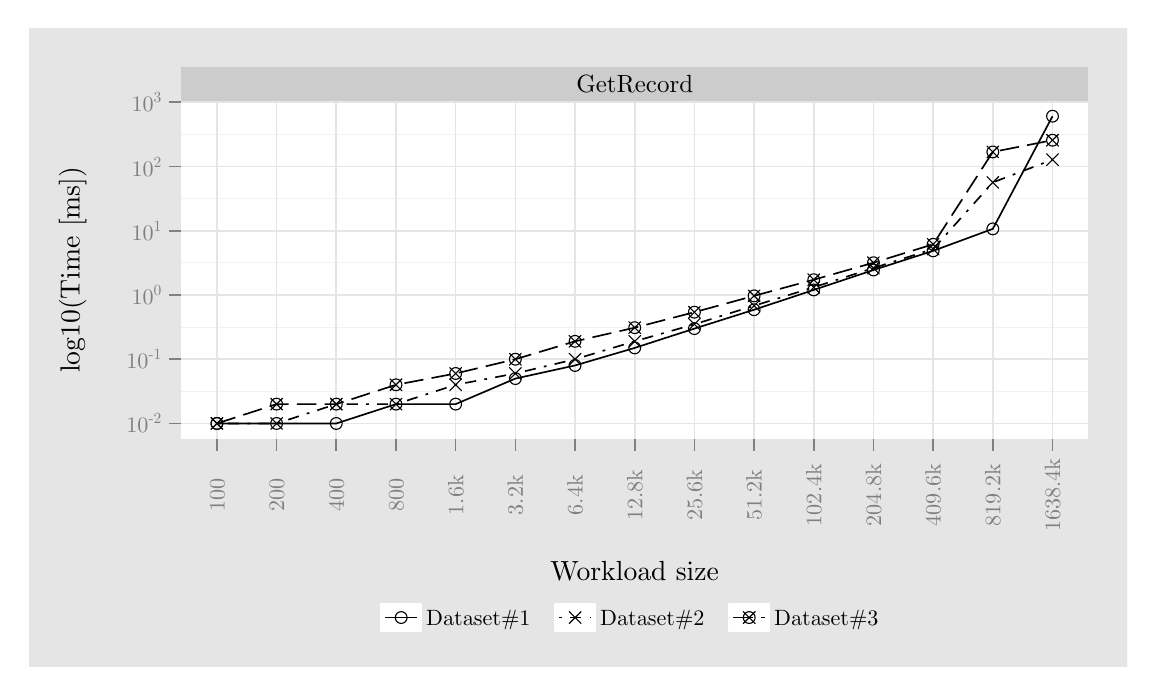
\begin{tikzpicture}[x=1pt,y=1pt]
\definecolor[named]{fillColor}{rgb}{1.00,1.00,1.00}
\path[use as bounding box,fill=fillColor,fill opacity=0.00] (0,0) rectangle (397.48,231.26);
\begin{scope}
\path[clip] (  0.00,  0.00) rectangle (397.48,231.26);
\definecolor[named]{drawColor}{rgb}{1.00,1.00,1.00}
\definecolor[named]{fillColor}{rgb}{0.90,0.90,0.90}

\path[draw=drawColor,line width= 0.6pt,line join=round,line cap=round,fill=fillColor] (  0.00,  0.00) rectangle (397.48,231.26);
\end{scope}
\begin{scope}
\path[clip] ( 55.45, 82.69) rectangle (383.26,204.82);
\definecolor[named]{fillColor}{rgb}{1.00,1.00,1.00}

\path[fill=fillColor] ( 55.45, 82.69) rectangle (383.26,204.82);
\definecolor[named]{drawColor}{rgb}{0.95,0.95,0.95}

\path[draw=drawColor,line width= 0.3pt,line join=round] ( 55.45, 99.85) --
	(383.26, 99.85);

\path[draw=drawColor,line width= 0.3pt,line join=round] ( 55.45,123.05) --
	(383.26,123.05);

\path[draw=drawColor,line width= 0.3pt,line join=round] ( 55.45,146.26) --
	(383.26,146.26);

\path[draw=drawColor,line width= 0.3pt,line join=round] ( 55.45,169.47) --
	(383.26,169.47);

\path[draw=drawColor,line width= 0.3pt,line join=round] ( 55.45,192.68) --
	(383.26,192.68);
\definecolor[named]{drawColor}{rgb}{0.90,0.90,0.90}

\path[draw=drawColor,line width= 0.6pt,line join=round] ( 55.45, 88.24) --
	(383.26, 88.24);

\path[draw=drawColor,line width= 0.6pt,line join=round] ( 55.45,111.45) --
	(383.26,111.45);

\path[draw=drawColor,line width= 0.6pt,line join=round] ( 55.45,134.66) --
	(383.26,134.66);

\path[draw=drawColor,line width= 0.6pt,line join=round] ( 55.45,157.86) --
	(383.26,157.86);

\path[draw=drawColor,line width= 0.6pt,line join=round] ( 55.45,181.07) --
	(383.26,181.07);

\path[draw=drawColor,line width= 0.6pt,line join=round] ( 55.45,204.28) --
	(383.26,204.28);

\path[draw=drawColor,line width= 0.6pt,line join=round] ( 68.39, 82.69) --
	( 68.39,204.82);

\path[draw=drawColor,line width= 0.6pt,line join=round] ( 89.95, 82.69) --
	( 89.95,204.82);

\path[draw=drawColor,line width= 0.6pt,line join=round] (111.52, 82.69) --
	(111.52,204.82);

\path[draw=drawColor,line width= 0.6pt,line join=round] (133.09, 82.69) --
	(133.09,204.82);

\path[draw=drawColor,line width= 0.6pt,line join=round] (154.65, 82.69) --
	(154.65,204.82);

\path[draw=drawColor,line width= 0.6pt,line join=round] (176.22, 82.69) --
	(176.22,204.82);

\path[draw=drawColor,line width= 0.6pt,line join=round] (197.79, 82.69) --
	(197.79,204.82);

\path[draw=drawColor,line width= 0.6pt,line join=round] (219.35, 82.69) --
	(219.35,204.82);

\path[draw=drawColor,line width= 0.6pt,line join=round] (240.92, 82.69) --
	(240.92,204.82);

\path[draw=drawColor,line width= 0.6pt,line join=round] (262.49, 82.69) --
	(262.49,204.82);

\path[draw=drawColor,line width= 0.6pt,line join=round] (284.05, 82.69) --
	(284.05,204.82);

\path[draw=drawColor,line width= 0.6pt,line join=round] (305.62, 82.69) --
	(305.62,204.82);

\path[draw=drawColor,line width= 0.6pt,line join=round] (327.19, 82.69) --
	(327.19,204.82);

\path[draw=drawColor,line width= 0.6pt,line join=round] (348.75, 82.69) --
	(348.75,204.82);

\path[draw=drawColor,line width= 0.6pt,line join=round] (370.32, 82.69) --
	(370.32,204.82);
\definecolor[named]{drawColor}{rgb}{0.00,0.00,0.00}

\path[draw=drawColor,line width= 0.6pt,line join=round] ( 68.39, 88.24) --
	( 89.95, 88.24) --
	(111.52, 88.24) --
	(133.09, 95.23) --
	(154.65, 95.23) --
	(176.22,104.46) --
	(197.79,109.20) --
	(219.35,115.54) --
	(240.92,122.52) --
	(262.49,129.34) --
	(284.05,136.49) --
	(305.62,143.69) --
	(327.19,150.61) --
	(348.75,158.56) --
	(370.32,199.27);

\path[draw=drawColor,line width= 0.6pt,dash pattern=on 1pt off 3pt on 4pt off 3pt ,line join=round] ( 68.39, 88.24) --
	( 89.95, 88.24) --
	(111.52, 95.23) --
	(133.09, 95.23) --
	(154.65,102.21) --
	(176.22,106.30) --
	(197.79,111.45) --
	(219.35,117.92) --
	(240.92,124.08) --
	(262.49,130.77) --
	(284.05,137.45) --
	(305.62,144.40) --
	(327.19,151.27) --
	(348.75,175.34) --
	(370.32,183.56);

\path[draw=drawColor,line width= 0.6pt,dash pattern=on 7pt off 3pt ,line join=round] ( 68.39, 88.24) --
	( 89.95, 95.23) --
	(111.52, 95.23) --
	(133.09,102.21) --
	(154.65,106.30) --
	(176.22,111.45) --
	(197.79,117.92) --
	(219.35,122.85) --
	(240.92,128.45) --
	(262.49,134.35) --
	(284.05,140.18) --
	(305.62,146.32) --
	(327.19,152.98) --
	(348.75,186.35) --
	(370.32,190.59);

\path[draw=drawColor,line width= 0.4pt,line join=round,line cap=round] ( 68.39, 88.24) circle (  2.13);

\path[draw=drawColor,line width= 0.4pt,line join=round,line cap=round] ( 89.95, 88.24) circle (  2.13);

\path[draw=drawColor,line width= 0.4pt,line join=round,line cap=round] (111.52, 88.24) circle (  2.13);

\path[draw=drawColor,line width= 0.4pt,line join=round,line cap=round] (133.09, 95.23) circle (  2.13);

\path[draw=drawColor,line width= 0.4pt,line join=round,line cap=round] (154.65, 95.23) circle (  2.13);

\path[draw=drawColor,line width= 0.4pt,line join=round,line cap=round] (176.22,104.46) circle (  2.13);

\path[draw=drawColor,line width= 0.4pt,line join=round,line cap=round] (197.79,109.20) circle (  2.13);

\path[draw=drawColor,line width= 0.4pt,line join=round,line cap=round] (219.35,115.54) circle (  2.13);

\path[draw=drawColor,line width= 0.4pt,line join=round,line cap=round] (240.92,122.52) circle (  2.13);

\path[draw=drawColor,line width= 0.4pt,line join=round,line cap=round] (262.49,129.34) circle (  2.13);

\path[draw=drawColor,line width= 0.4pt,line join=round,line cap=round] (284.05,136.49) circle (  2.13);

\path[draw=drawColor,line width= 0.4pt,line join=round,line cap=round] (305.62,143.69) circle (  2.13);

\path[draw=drawColor,line width= 0.4pt,line join=round,line cap=round] (327.19,150.61) circle (  2.13);

\path[draw=drawColor,line width= 0.4pt,line join=round,line cap=round] (348.75,158.56) circle (  2.13);

\path[draw=drawColor,line width= 0.4pt,line join=round,line cap=round] (370.32,199.27) circle (  2.13);

\path[draw=drawColor,line width= 0.4pt,line join=round,line cap=round] ( 68.39, 88.24) circle (  2.13);

\path[draw=drawColor,line width= 0.4pt,line join=round,line cap=round] ( 66.25, 86.11) -- ( 70.52, 90.38);

\path[draw=drawColor,line width= 0.4pt,line join=round,line cap=round] ( 66.25, 90.38) -- ( 70.52, 86.11);

\path[draw=drawColor,line width= 0.4pt,line join=round,line cap=round] ( 89.95, 95.23) circle (  2.13);

\path[draw=drawColor,line width= 0.4pt,line join=round,line cap=round] ( 87.82, 93.09) -- ( 92.09, 97.36);

\path[draw=drawColor,line width= 0.4pt,line join=round,line cap=round] ( 87.82, 97.36) -- ( 92.09, 93.09);

\path[draw=drawColor,line width= 0.4pt,line join=round,line cap=round] (111.52, 95.23) circle (  2.13);

\path[draw=drawColor,line width= 0.4pt,line join=round,line cap=round] (109.39, 93.09) -- (113.66, 97.36);

\path[draw=drawColor,line width= 0.4pt,line join=round,line cap=round] (109.39, 97.36) -- (113.66, 93.09);

\path[draw=drawColor,line width= 0.4pt,line join=round,line cap=round] (133.09,102.21) circle (  2.13);

\path[draw=drawColor,line width= 0.4pt,line join=round,line cap=round] (130.95,100.08) -- (135.22,104.35);

\path[draw=drawColor,line width= 0.4pt,line join=round,line cap=round] (130.95,104.35) -- (135.22,100.08);

\path[draw=drawColor,line width= 0.4pt,line join=round,line cap=round] (154.65,106.30) circle (  2.13);

\path[draw=drawColor,line width= 0.4pt,line join=round,line cap=round] (152.52,104.17) -- (156.79,108.43);

\path[draw=drawColor,line width= 0.4pt,line join=round,line cap=round] (152.52,108.43) -- (156.79,104.17);

\path[draw=drawColor,line width= 0.4pt,line join=round,line cap=round] (176.22,111.45) circle (  2.13);

\path[draw=drawColor,line width= 0.4pt,line join=round,line cap=round] (174.09,109.32) -- (178.35,113.58);

\path[draw=drawColor,line width= 0.4pt,line join=round,line cap=round] (174.09,113.58) -- (178.35,109.32);

\path[draw=drawColor,line width= 0.4pt,line join=round,line cap=round] (197.79,117.92) circle (  2.13);

\path[draw=drawColor,line width= 0.4pt,line join=round,line cap=round] (195.65,115.78) -- (199.92,120.05);

\path[draw=drawColor,line width= 0.4pt,line join=round,line cap=round] (195.65,120.05) -- (199.92,115.78);

\path[draw=drawColor,line width= 0.4pt,line join=round,line cap=round] (219.35,122.85) circle (  2.13);

\path[draw=drawColor,line width= 0.4pt,line join=round,line cap=round] (217.22,120.72) -- (221.49,124.99);

\path[draw=drawColor,line width= 0.4pt,line join=round,line cap=round] (217.22,124.99) -- (221.49,120.72);

\path[draw=drawColor,line width= 0.4pt,line join=round,line cap=round] (240.92,128.45) circle (  2.13);

\path[draw=drawColor,line width= 0.4pt,line join=round,line cap=round] (238.79,126.31) -- (243.05,130.58);

\path[draw=drawColor,line width= 0.4pt,line join=round,line cap=round] (238.79,130.58) -- (243.05,126.31);

\path[draw=drawColor,line width= 0.4pt,line join=round,line cap=round] (262.49,134.35) circle (  2.13);

\path[draw=drawColor,line width= 0.4pt,line join=round,line cap=round] (260.35,132.22) -- (264.62,136.48);

\path[draw=drawColor,line width= 0.4pt,line join=round,line cap=round] (260.35,136.48) -- (264.62,132.22);

\path[draw=drawColor,line width= 0.4pt,line join=round,line cap=round] (284.05,140.18) circle (  2.13);

\path[draw=drawColor,line width= 0.4pt,line join=round,line cap=round] (281.92,138.05) -- (286.19,142.32);

\path[draw=drawColor,line width= 0.4pt,line join=round,line cap=round] (281.92,142.32) -- (286.19,138.05);

\path[draw=drawColor,line width= 0.4pt,line join=round,line cap=round] (305.62,146.32) circle (  2.13);

\path[draw=drawColor,line width= 0.4pt,line join=round,line cap=round] (303.49,144.18) -- (307.75,148.45);

\path[draw=drawColor,line width= 0.4pt,line join=round,line cap=round] (303.49,148.45) -- (307.75,144.18);

\path[draw=drawColor,line width= 0.4pt,line join=round,line cap=round] (327.19,152.98) circle (  2.13);

\path[draw=drawColor,line width= 0.4pt,line join=round,line cap=round] (325.05,150.85) -- (329.32,155.11);

\path[draw=drawColor,line width= 0.4pt,line join=round,line cap=round] (325.05,155.11) -- (329.32,150.85);

\path[draw=drawColor,line width= 0.4pt,line join=round,line cap=round] (348.75,186.35) circle (  2.13);

\path[draw=drawColor,line width= 0.4pt,line join=round,line cap=round] (346.62,184.22) -- (350.89,188.49);

\path[draw=drawColor,line width= 0.4pt,line join=round,line cap=round] (346.62,188.49) -- (350.89,184.22);

\path[draw=drawColor,line width= 0.4pt,line join=round,line cap=round] (370.32,190.59) circle (  2.13);

\path[draw=drawColor,line width= 0.4pt,line join=round,line cap=round] (368.18,188.46) -- (372.45,192.72);

\path[draw=drawColor,line width= 0.4pt,line join=round,line cap=round] (368.18,192.72) -- (372.45,188.46);

\path[draw=drawColor,line width= 0.4pt,line join=round,line cap=round,fill=fillColor] ( 66.25, 86.11) -- ( 70.52, 90.38);

\path[draw=drawColor,line width= 0.4pt,line join=round,line cap=round,fill=fillColor] ( 66.25, 90.38) -- ( 70.52, 86.11);

\path[draw=drawColor,line width= 0.4pt,line join=round,line cap=round,fill=fillColor] ( 87.82, 86.11) -- ( 92.09, 90.38);

\path[draw=drawColor,line width= 0.4pt,line join=round,line cap=round,fill=fillColor] ( 87.82, 90.38) -- ( 92.09, 86.11);

\path[draw=drawColor,line width= 0.4pt,line join=round,line cap=round,fill=fillColor] (109.39, 93.09) -- (113.66, 97.36);

\path[draw=drawColor,line width= 0.4pt,line join=round,line cap=round,fill=fillColor] (109.39, 97.36) -- (113.66, 93.09);

\path[draw=drawColor,line width= 0.4pt,line join=round,line cap=round,fill=fillColor] (130.95, 93.09) -- (135.22, 97.36);

\path[draw=drawColor,line width= 0.4pt,line join=round,line cap=round,fill=fillColor] (130.95, 97.36) -- (135.22, 93.09);

\path[draw=drawColor,line width= 0.4pt,line join=round,line cap=round,fill=fillColor] (152.52,100.08) -- (156.79,104.35);

\path[draw=drawColor,line width= 0.4pt,line join=round,line cap=round,fill=fillColor] (152.52,104.35) -- (156.79,100.08);

\path[draw=drawColor,line width= 0.4pt,line join=round,line cap=round,fill=fillColor] (174.09,104.17) -- (178.35,108.43);

\path[draw=drawColor,line width= 0.4pt,line join=round,line cap=round,fill=fillColor] (174.09,108.43) -- (178.35,104.17);

\path[draw=drawColor,line width= 0.4pt,line join=round,line cap=round,fill=fillColor] (195.65,109.32) -- (199.92,113.58);

\path[draw=drawColor,line width= 0.4pt,line join=round,line cap=round,fill=fillColor] (195.65,113.58) -- (199.92,109.32);

\path[draw=drawColor,line width= 0.4pt,line join=round,line cap=round,fill=fillColor] (217.22,115.78) -- (221.49,120.05);

\path[draw=drawColor,line width= 0.4pt,line join=round,line cap=round,fill=fillColor] (217.22,120.05) -- (221.49,115.78);

\path[draw=drawColor,line width= 0.4pt,line join=round,line cap=round,fill=fillColor] (238.79,121.94) -- (243.05,126.21);

\path[draw=drawColor,line width= 0.4pt,line join=round,line cap=round,fill=fillColor] (238.79,126.21) -- (243.05,121.94);

\path[draw=drawColor,line width= 0.4pt,line join=round,line cap=round,fill=fillColor] (260.35,128.64) -- (264.62,132.90);

\path[draw=drawColor,line width= 0.4pt,line join=round,line cap=round,fill=fillColor] (260.35,132.90) -- (264.62,128.64);

\path[draw=drawColor,line width= 0.4pt,line join=round,line cap=round,fill=fillColor] (281.92,135.32) -- (286.19,139.59);

\path[draw=drawColor,line width= 0.4pt,line join=round,line cap=round,fill=fillColor] (281.92,139.59) -- (286.19,135.32);

\path[draw=drawColor,line width= 0.4pt,line join=round,line cap=round,fill=fillColor] (303.49,142.27) -- (307.75,146.54);

\path[draw=drawColor,line width= 0.4pt,line join=round,line cap=round,fill=fillColor] (303.49,146.54) -- (307.75,142.27);

\path[draw=drawColor,line width= 0.4pt,line join=round,line cap=round,fill=fillColor] (325.05,149.14) -- (329.32,153.41);

\path[draw=drawColor,line width= 0.4pt,line join=round,line cap=round,fill=fillColor] (325.05,153.41) -- (329.32,149.14);

\path[draw=drawColor,line width= 0.4pt,line join=round,line cap=round,fill=fillColor] (346.62,173.21) -- (350.89,177.48);

\path[draw=drawColor,line width= 0.4pt,line join=round,line cap=round,fill=fillColor] (346.62,177.48) -- (350.89,173.21);

\path[draw=drawColor,line width= 0.4pt,line join=round,line cap=round,fill=fillColor] (368.18,181.43) -- (372.45,185.69);

\path[draw=drawColor,line width= 0.4pt,line join=round,line cap=round,fill=fillColor] (368.18,185.69) -- (372.45,181.43);
\end{scope}
\begin{scope}
\path[clip] (  0.00,  0.00) rectangle (397.48,231.26);
\definecolor[named]{fillColor}{rgb}{0.80,0.80,0.80}

\path[fill=fillColor] ( 55.45,204.82) rectangle (383.26,217.04);
\definecolor[named]{drawColor}{rgb}{0.00,0.00,0.00}

\node[text=drawColor,anchor=base,inner sep=0pt, outer sep=0pt, scale=  0.90] at (219.35,207.83) {GetRecord};
\end{scope}
\begin{scope}
\path[clip] (  0.00,  0.00) rectangle (397.48,231.26);
\definecolor[named]{drawColor}{rgb}{0.50,0.50,0.50}

\node[text=drawColor,anchor=base west,inner sep=0pt, outer sep=0pt, scale=  0.80] at ( 35.67, 84.81) {10};

\node[text=drawColor,anchor=base west,inner sep=0pt, outer sep=0pt, scale=  0.56] at ( 43.67, 88.08) {-};

\node[text=drawColor,anchor=base west,inner sep=0pt, outer sep=0pt, scale=  0.56] at ( 45.54, 88.08) {2};

\node[text=drawColor,anchor=base west,inner sep=0pt, outer sep=0pt, scale=  0.80] at ( 35.67,108.02) {10};

\node[text=drawColor,anchor=base west,inner sep=0pt, outer sep=0pt, scale=  0.56] at ( 43.67,111.29) {-};

\node[text=drawColor,anchor=base west,inner sep=0pt, outer sep=0pt, scale=  0.56] at ( 45.54,111.29) {1};

\node[text=drawColor,anchor=base west,inner sep=0pt, outer sep=0pt, scale=  0.80] at ( 37.54,131.22) {10};

\node[text=drawColor,anchor=base west,inner sep=0pt, outer sep=0pt, scale=  0.56] at ( 45.54,134.50) {0};

\node[text=drawColor,anchor=base west,inner sep=0pt, outer sep=0pt, scale=  0.80] at ( 37.54,154.43) {10};

\node[text=drawColor,anchor=base west,inner sep=0pt, outer sep=0pt, scale=  0.56] at ( 45.54,157.70) {1};

\node[text=drawColor,anchor=base west,inner sep=0pt, outer sep=0pt, scale=  0.80] at ( 37.54,177.64) {10};

\node[text=drawColor,anchor=base west,inner sep=0pt, outer sep=0pt, scale=  0.56] at ( 45.54,180.91) {2};

\node[text=drawColor,anchor=base west,inner sep=0pt, outer sep=0pt, scale=  0.80] at ( 37.54,200.85) {10};

\node[text=drawColor,anchor=base west,inner sep=0pt, outer sep=0pt, scale=  0.56] at ( 45.54,204.12) {3};
\end{scope}
\begin{scope}
\path[clip] (  0.00,  0.00) rectangle (397.48,231.26);
\definecolor[named]{drawColor}{rgb}{0.50,0.50,0.50}

\path[draw=drawColor,line width= 0.6pt,line join=round] ( 51.18, 88.24) --
	( 55.45, 88.24);

\path[draw=drawColor,line width= 0.6pt,line join=round] ( 51.18,111.45) --
	( 55.45,111.45);

\path[draw=drawColor,line width= 0.6pt,line join=round] ( 51.18,134.66) --
	( 55.45,134.66);

\path[draw=drawColor,line width= 0.6pt,line join=round] ( 51.18,157.86) --
	( 55.45,157.86);

\path[draw=drawColor,line width= 0.6pt,line join=round] ( 51.18,181.07) --
	( 55.45,181.07);

\path[draw=drawColor,line width= 0.6pt,line join=round] ( 51.18,204.28) --
	( 55.45,204.28);
\end{scope}
\begin{scope}
\path[clip] (  0.00,  0.00) rectangle (397.48,231.26);
\definecolor[named]{drawColor}{rgb}{0.50,0.50,0.50}

\path[draw=drawColor,line width= 0.6pt,line join=round] ( 68.39, 78.42) --
	( 68.39, 82.69);

\path[draw=drawColor,line width= 0.6pt,line join=round] ( 89.95, 78.42) --
	( 89.95, 82.69);

\path[draw=drawColor,line width= 0.6pt,line join=round] (111.52, 78.42) --
	(111.52, 82.69);

\path[draw=drawColor,line width= 0.6pt,line join=round] (133.09, 78.42) --
	(133.09, 82.69);

\path[draw=drawColor,line width= 0.6pt,line join=round] (154.65, 78.42) --
	(154.65, 82.69);

\path[draw=drawColor,line width= 0.6pt,line join=round] (176.22, 78.42) --
	(176.22, 82.69);

\path[draw=drawColor,line width= 0.6pt,line join=round] (197.79, 78.42) --
	(197.79, 82.69);

\path[draw=drawColor,line width= 0.6pt,line join=round] (219.35, 78.42) --
	(219.35, 82.69);

\path[draw=drawColor,line width= 0.6pt,line join=round] (240.92, 78.42) --
	(240.92, 82.69);

\path[draw=drawColor,line width= 0.6pt,line join=round] (262.49, 78.42) --
	(262.49, 82.69);

\path[draw=drawColor,line width= 0.6pt,line join=round] (284.05, 78.42) --
	(284.05, 82.69);

\path[draw=drawColor,line width= 0.6pt,line join=round] (305.62, 78.42) --
	(305.62, 82.69);

\path[draw=drawColor,line width= 0.6pt,line join=round] (327.19, 78.42) --
	(327.19, 82.69);

\path[draw=drawColor,line width= 0.6pt,line join=round] (348.75, 78.42) --
	(348.75, 82.69);

\path[draw=drawColor,line width= 0.6pt,line join=round] (370.32, 78.42) --
	(370.32, 82.69);
\end{scope}
\begin{scope}
\path[clip] (  0.00,  0.00) rectangle (397.48,231.26);
\definecolor[named]{drawColor}{rgb}{0.50,0.50,0.50}

\node[text=drawColor,rotate= 90.00,anchor=base,inner sep=0pt, outer sep=0pt, scale=  0.80] at ( 71.14, 62.36) {100};

\node[text=drawColor,rotate= 90.00,anchor=base,inner sep=0pt, outer sep=0pt, scale=  0.80] at ( 92.71, 62.36) {200};

\node[text=drawColor,rotate= 90.00,anchor=base,inner sep=0pt, outer sep=0pt, scale=  0.80] at (114.28, 62.36) {400};

\node[text=drawColor,rotate= 90.00,anchor=base,inner sep=0pt, outer sep=0pt, scale=  0.80] at (135.84, 62.36) {800};

\node[text=drawColor,rotate= 90.00,anchor=base,inner sep=0pt, outer sep=0pt, scale=  0.80] at (157.41, 62.36) {1.6k};

\node[text=drawColor,rotate= 90.00,anchor=base,inner sep=0pt, outer sep=0pt, scale=  0.80] at (178.98, 62.36) {3.2k};

\node[text=drawColor,rotate= 90.00,anchor=base,inner sep=0pt, outer sep=0pt, scale=  0.80] at (200.54, 62.36) {6.4k};

\node[text=drawColor,rotate= 90.00,anchor=base,inner sep=0pt, outer sep=0pt, scale=  0.80] at (222.11, 62.36) {12.8k};

\node[text=drawColor,rotate= 90.00,anchor=base,inner sep=0pt, outer sep=0pt, scale=  0.80] at (243.67, 62.36) {25.6k};

\node[text=drawColor,rotate= 90.00,anchor=base,inner sep=0pt, outer sep=0pt, scale=  0.80] at (265.24, 62.36) {51.2k};

\node[text=drawColor,rotate= 90.00,anchor=base,inner sep=0pt, outer sep=0pt, scale=  0.80] at (286.81, 62.36) {102.4k};

\node[text=drawColor,rotate= 90.00,anchor=base,inner sep=0pt, outer sep=0pt, scale=  0.80] at (308.37, 62.36) {204.8k};

\node[text=drawColor,rotate= 90.00,anchor=base,inner sep=0pt, outer sep=0pt, scale=  0.80] at (329.94, 62.36) {409.6k};

\node[text=drawColor,rotate= 90.00,anchor=base,inner sep=0pt, outer sep=0pt, scale=  0.80] at (351.51, 62.36) {819.2k};

\node[text=drawColor,rotate= 90.00,anchor=base,inner sep=0pt, outer sep=0pt, scale=  0.80] at (373.07, 62.36) {1638.4k};
\end{scope}
\begin{scope}
\path[clip] (  0.00,  0.00) rectangle (397.48,231.26);
\definecolor[named]{drawColor}{rgb}{0.00,0.00,0.00}

\node[text=drawColor,anchor=base,inner sep=0pt, outer sep=0pt, scale=  1.00] at (219.35, 31.41) {Workload size};
\end{scope}
\begin{scope}
\path[clip] (  0.00,  0.00) rectangle (397.48,231.26);
\definecolor[named]{drawColor}{rgb}{0.00,0.00,0.00}

\node[text=drawColor,rotate= 90.00,anchor=base,inner sep=0pt, outer sep=0pt, scale=  1.00] at ( 18.80,143.75) {log10(Time [ms])};
\end{scope}
\begin{scope}
\path[clip] (  0.00,  0.00) rectangle (397.48,231.26);
\definecolor[named]{fillColor}{rgb}{0.90,0.90,0.90}

\path[fill=fillColor] (119.86,  8.87) rectangle (318.84, 27.36);
\end{scope}
\begin{scope}
\path[clip] (  0.00,  0.00) rectangle (397.48,231.26);
\definecolor[named]{drawColor}{rgb}{1.00,1.00,1.00}
\definecolor[named]{fillColor}{rgb}{1.00,1.00,1.00}

\path[draw=drawColor,line width= 0.6pt,line join=round,line cap=round,fill=fillColor] (127.74, 13.14) rectangle (142.20, 23.09);
\end{scope}
\begin{scope}
\path[clip] (  0.00,  0.00) rectangle (397.48,231.26);
\definecolor[named]{drawColor}{rgb}{0.00,0.00,0.00}

\path[draw=drawColor,line width= 0.6pt,line join=round] (129.19, 18.11) -- (140.75, 18.11);
\end{scope}
\begin{scope}
\path[clip] (  0.00,  0.00) rectangle (397.48,231.26);
\definecolor[named]{drawColor}{rgb}{0.00,0.00,0.00}

\path[draw=drawColor,line width= 0.4pt,line join=round,line cap=round] (134.97, 18.11) circle (  2.13);
\end{scope}
\begin{scope}
\path[clip] (  0.00,  0.00) rectangle (397.48,231.26);
\definecolor[named]{drawColor}{rgb}{1.00,1.00,1.00}
\definecolor[named]{fillColor}{rgb}{1.00,1.00,1.00}

\path[draw=drawColor,line width= 0.6pt,line join=round,line cap=round,fill=fillColor] (190.62, 13.14) rectangle (205.08, 23.09);
\end{scope}
\begin{scope}
\path[clip] (  0.00,  0.00) rectangle (397.48,231.26);
\definecolor[named]{drawColor}{rgb}{0.00,0.00,0.00}

\path[draw=drawColor,line width= 0.6pt,dash pattern=on 1pt off 3pt on 4pt off 3pt ,line join=round] (192.07, 18.11) -- (203.63, 18.11);
\end{scope}
\begin{scope}
\path[clip] (  0.00,  0.00) rectangle (397.48,231.26);
\definecolor[named]{drawColor}{rgb}{0.00,0.00,0.00}
\definecolor[named]{fillColor}{rgb}{1.00,1.00,1.00}

\path[draw=drawColor,line width= 0.4pt,line join=round,line cap=round,fill=fillColor] (195.72, 15.98) -- (199.98, 20.25);

\path[draw=drawColor,line width= 0.4pt,line join=round,line cap=round,fill=fillColor] (195.72, 20.25) -- (199.98, 15.98);
\end{scope}
\begin{scope}
\path[clip] (  0.00,  0.00) rectangle (397.48,231.26);
\definecolor[named]{drawColor}{rgb}{1.00,1.00,1.00}
\definecolor[named]{fillColor}{rgb}{1.00,1.00,1.00}

\path[draw=drawColor,line width= 0.6pt,line join=round,line cap=round,fill=fillColor] (253.50, 13.14) rectangle (267.96, 23.09);
\end{scope}
\begin{scope}
\path[clip] (  0.00,  0.00) rectangle (397.48,231.26);
\definecolor[named]{drawColor}{rgb}{0.00,0.00,0.00}

\path[draw=drawColor,line width= 0.6pt,dash pattern=on 7pt off 3pt ,line join=round] (254.95, 18.11) -- (266.51, 18.11);
\end{scope}
\begin{scope}
\path[clip] (  0.00,  0.00) rectangle (397.48,231.26);
\definecolor[named]{drawColor}{rgb}{0.00,0.00,0.00}

\path[draw=drawColor,line width= 0.4pt,line join=round,line cap=round] (260.73, 18.11) circle (  2.13);

\path[draw=drawColor,line width= 0.4pt,line join=round,line cap=round] (258.60, 15.98) -- (262.86, 20.25);

\path[draw=drawColor,line width= 0.4pt,line join=round,line cap=round] (258.60, 20.25) -- (262.86, 15.98);
\end{scope}
\begin{scope}
\path[clip] (  0.00,  0.00) rectangle (397.48,231.26);
\definecolor[named]{drawColor}{rgb}{0.00,0.00,0.00}

\node[text=drawColor,anchor=base west,inner sep=0pt, outer sep=0pt, scale=  0.80] at (144.00, 15.36) {Dataset\#1 $\;\;$};
\end{scope}
\begin{scope}
\path[clip] (  0.00,  0.00) rectangle (397.48,231.26);
\definecolor[named]{drawColor}{rgb}{0.00,0.00,0.00}

\node[text=drawColor,anchor=base west,inner sep=0pt, outer sep=0pt, scale=  0.80] at (206.88, 15.36) {Dataset\#2 $\;\;$};
\end{scope}
\begin{scope}
\path[clip] (  0.00,  0.00) rectangle (397.48,231.26);
\definecolor[named]{drawColor}{rgb}{0.00,0.00,0.00}

\node[text=drawColor,anchor=base west,inner sep=0pt, outer sep=0pt, scale=  0.80] at (269.76, 15.36) {Dataset\#3 $\;\;$};
\end{scope}
\end{tikzpicture}

 }
 \caption[OAI-PMH data provider\index{OAI-PMH!Data Provider} GetRecord\index{OAI-PMH!Verbs!GetRecord} performance]{OAI-PMH data provider\index{OAI-PMH!Data Provider} GetRecord\index{OAI-PMH!Verbs!GetRecord} performance}
 \label{fig:experimentation:performance:oaipmh:getrecord-level}
\end{figure}


\begin{figure}
 \centering
 \framebox[\textwidth]{%
% Created by tikzDevice version 0.6.2-92-0ad2792 on 2013-03-23 23:04:44
% !TEX encoding = UTF-8 Unicode
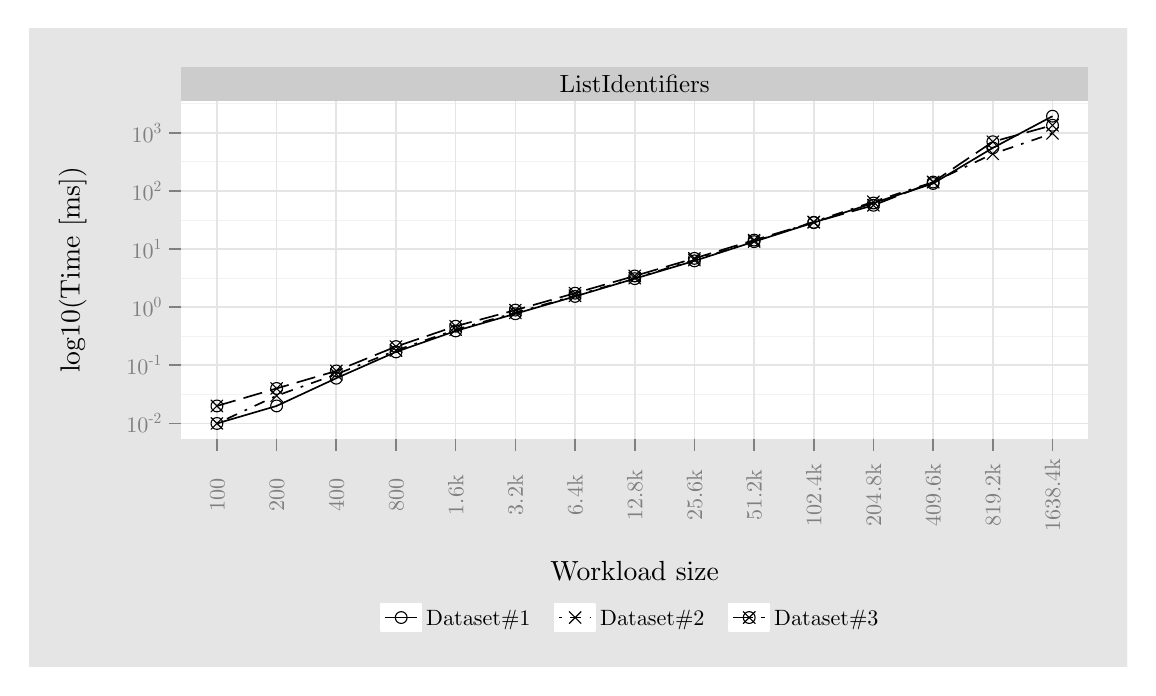
\begin{tikzpicture}[x=1pt,y=1pt]
\definecolor[named]{fillColor}{rgb}{1.00,1.00,1.00}
\path[use as bounding box,fill=fillColor,fill opacity=0.00] (0,0) rectangle (397.48,231.26);
\begin{scope}
\path[clip] (  0.00,  0.00) rectangle (397.48,231.26);
\definecolor[named]{drawColor}{rgb}{1.00,1.00,1.00}
\definecolor[named]{fillColor}{rgb}{0.90,0.90,0.90}

\path[draw=drawColor,line width= 0.6pt,line join=round,line cap=round,fill=fillColor] (  0.00,  0.00) rectangle (397.48,231.26);
\end{scope}
\begin{scope}
\path[clip] ( 55.45, 82.69) rectangle (383.26,204.82);
\definecolor[named]{fillColor}{rgb}{1.00,1.00,1.00}

\path[fill=fillColor] ( 55.45, 82.69) rectangle (383.26,204.82);
\definecolor[named]{drawColor}{rgb}{0.95,0.95,0.95}

\path[draw=drawColor,line width= 0.3pt,line join=round] ( 55.45, 98.75) --
	(383.26, 98.75);

\path[draw=drawColor,line width= 0.3pt,line join=round] ( 55.45,119.76) --
	(383.26,119.76);

\path[draw=drawColor,line width= 0.3pt,line join=round] ( 55.45,140.77) --
	(383.26,140.77);

\path[draw=drawColor,line width= 0.3pt,line join=round] ( 55.45,161.78) --
	(383.26,161.78);

\path[draw=drawColor,line width= 0.3pt,line join=round] ( 55.45,182.79) --
	(383.26,182.79);

\path[draw=drawColor,line width= 0.3pt,line join=round] ( 55.45,203.80) --
	(383.26,203.80);
\definecolor[named]{drawColor}{rgb}{0.90,0.90,0.90}

\path[draw=drawColor,line width= 0.6pt,line join=round] ( 55.45, 88.24) --
	(383.26, 88.24);

\path[draw=drawColor,line width= 0.6pt,line join=round] ( 55.45,109.25) --
	(383.26,109.25);

\path[draw=drawColor,line width= 0.6pt,line join=round] ( 55.45,130.26) --
	(383.26,130.26);

\path[draw=drawColor,line width= 0.6pt,line join=round] ( 55.45,151.28) --
	(383.26,151.28);

\path[draw=drawColor,line width= 0.6pt,line join=round] ( 55.45,172.29) --
	(383.26,172.29);

\path[draw=drawColor,line width= 0.6pt,line join=round] ( 55.45,193.30) --
	(383.26,193.30);

\path[draw=drawColor,line width= 0.6pt,line join=round] ( 68.39, 82.69) --
	( 68.39,204.82);

\path[draw=drawColor,line width= 0.6pt,line join=round] ( 89.95, 82.69) --
	( 89.95,204.82);

\path[draw=drawColor,line width= 0.6pt,line join=round] (111.52, 82.69) --
	(111.52,204.82);

\path[draw=drawColor,line width= 0.6pt,line join=round] (133.09, 82.69) --
	(133.09,204.82);

\path[draw=drawColor,line width= 0.6pt,line join=round] (154.65, 82.69) --
	(154.65,204.82);

\path[draw=drawColor,line width= 0.6pt,line join=round] (176.22, 82.69) --
	(176.22,204.82);

\path[draw=drawColor,line width= 0.6pt,line join=round] (197.79, 82.69) --
	(197.79,204.82);

\path[draw=drawColor,line width= 0.6pt,line join=round] (219.35, 82.69) --
	(219.35,204.82);

\path[draw=drawColor,line width= 0.6pt,line join=round] (240.92, 82.69) --
	(240.92,204.82);

\path[draw=drawColor,line width= 0.6pt,line join=round] (262.49, 82.69) --
	(262.49,204.82);

\path[draw=drawColor,line width= 0.6pt,line join=round] (284.05, 82.69) --
	(284.05,204.82);

\path[draw=drawColor,line width= 0.6pt,line join=round] (305.62, 82.69) --
	(305.62,204.82);

\path[draw=drawColor,line width= 0.6pt,line join=round] (327.19, 82.69) --
	(327.19,204.82);

\path[draw=drawColor,line width= 0.6pt,line join=round] (348.75, 82.69) --
	(348.75,204.82);

\path[draw=drawColor,line width= 0.6pt,line join=round] (370.32, 82.69) --
	(370.32,204.82);
\definecolor[named]{drawColor}{rgb}{0.00,0.00,0.00}

\path[draw=drawColor,line width= 0.6pt,line join=round] ( 68.39, 88.24) --
	( 89.95, 94.57) --
	(111.52,104.59) --
	(133.09,114.10) --
	(154.65,121.67) --
	(176.22,127.88) --
	(197.79,134.15) --
	(219.35,140.56) --
	(240.92,146.99) --
	(262.49,153.93) --
	(284.05,160.82) --
	(305.62,167.90) --
	(327.19,174.95) --
	(348.75,187.81) --
	(370.32,199.27);

\path[draw=drawColor,line width= 0.6pt,dash pattern=on 1pt off 3pt on 4pt off 3pt ,line join=round] ( 68.39, 88.24) --
	( 89.95, 98.27) --
	(111.52,106.00) --
	(133.09,114.62) --
	(154.65,122.13) --
	(176.22,128.23) --
	(197.79,134.38) --
	(219.35,140.76) --
	(240.92,147.30) --
	(262.49,153.98) --
	(284.05,161.11) --
	(305.62,168.35) --
	(327.19,175.45) --
	(348.75,185.65) --
	(370.32,193.06);

\path[draw=drawColor,line width= 0.6pt,dash pattern=on 7pt off 3pt ,line join=round] ( 68.39, 94.57) --
	( 89.95,100.89) --
	(111.52,107.22) --
	(133.09,116.02) --
	(154.65,123.38) --
	(176.22,129.20) --
	(197.79,135.32) --
	(219.35,141.54) --
	(240.92,147.89) --
	(262.49,154.50) --
	(284.05,160.92) --
	(305.62,167.08) --
	(327.19,175.48) --
	(348.75,190.04) --
	(370.32,195.99);

\path[draw=drawColor,line width= 0.4pt,line join=round,line cap=round] ( 68.39, 88.24) circle (  2.13);

\path[draw=drawColor,line width= 0.4pt,line join=round,line cap=round] ( 89.95, 94.57) circle (  2.13);

\path[draw=drawColor,line width= 0.4pt,line join=round,line cap=round] (111.52,104.59) circle (  2.13);

\path[draw=drawColor,line width= 0.4pt,line join=round,line cap=round] (133.09,114.10) circle (  2.13);

\path[draw=drawColor,line width= 0.4pt,line join=round,line cap=round] (154.65,121.67) circle (  2.13);

\path[draw=drawColor,line width= 0.4pt,line join=round,line cap=round] (176.22,127.88) circle (  2.13);

\path[draw=drawColor,line width= 0.4pt,line join=round,line cap=round] (197.79,134.15) circle (  2.13);

\path[draw=drawColor,line width= 0.4pt,line join=round,line cap=round] (219.35,140.56) circle (  2.13);

\path[draw=drawColor,line width= 0.4pt,line join=round,line cap=round] (240.92,146.99) circle (  2.13);

\path[draw=drawColor,line width= 0.4pt,line join=round,line cap=round] (262.49,153.93) circle (  2.13);

\path[draw=drawColor,line width= 0.4pt,line join=round,line cap=round] (284.05,160.82) circle (  2.13);

\path[draw=drawColor,line width= 0.4pt,line join=round,line cap=round] (305.62,167.90) circle (  2.13);

\path[draw=drawColor,line width= 0.4pt,line join=round,line cap=round] (327.19,174.95) circle (  2.13);

\path[draw=drawColor,line width= 0.4pt,line join=round,line cap=round] (348.75,187.81) circle (  2.13);

\path[draw=drawColor,line width= 0.4pt,line join=round,line cap=round] (370.32,199.27) circle (  2.13);

\path[draw=drawColor,line width= 0.4pt,line join=round,line cap=round] ( 68.39, 94.57) circle (  2.13);

\path[draw=drawColor,line width= 0.4pt,line join=round,line cap=round] ( 66.25, 92.43) -- ( 70.52, 96.70);

\path[draw=drawColor,line width= 0.4pt,line join=round,line cap=round] ( 66.25, 96.70) -- ( 70.52, 92.43);

\path[draw=drawColor,line width= 0.4pt,line join=round,line cap=round] ( 89.95,100.89) circle (  2.13);

\path[draw=drawColor,line width= 0.4pt,line join=round,line cap=round] ( 87.82, 98.76) -- ( 92.09,103.03);

\path[draw=drawColor,line width= 0.4pt,line join=round,line cap=round] ( 87.82,103.03) -- ( 92.09, 98.76);

\path[draw=drawColor,line width= 0.4pt,line join=round,line cap=round] (111.52,107.22) circle (  2.13);

\path[draw=drawColor,line width= 0.4pt,line join=round,line cap=round] (109.39,105.08) -- (113.66,109.35);

\path[draw=drawColor,line width= 0.4pt,line join=round,line cap=round] (109.39,109.35) -- (113.66,105.08);

\path[draw=drawColor,line width= 0.4pt,line join=round,line cap=round] (133.09,116.02) circle (  2.13);

\path[draw=drawColor,line width= 0.4pt,line join=round,line cap=round] (130.95,113.89) -- (135.22,118.16);

\path[draw=drawColor,line width= 0.4pt,line join=round,line cap=round] (130.95,118.16) -- (135.22,113.89);

\path[draw=drawColor,line width= 0.4pt,line join=round,line cap=round] (154.65,123.38) circle (  2.13);

\path[draw=drawColor,line width= 0.4pt,line join=round,line cap=round] (152.52,121.24) -- (156.79,125.51);

\path[draw=drawColor,line width= 0.4pt,line join=round,line cap=round] (152.52,125.51) -- (156.79,121.24);

\path[draw=drawColor,line width= 0.4pt,line join=round,line cap=round] (176.22,129.20) circle (  2.13);

\path[draw=drawColor,line width= 0.4pt,line join=round,line cap=round] (174.09,127.07) -- (178.35,131.34);

\path[draw=drawColor,line width= 0.4pt,line join=round,line cap=round] (174.09,131.34) -- (178.35,127.07);

\path[draw=drawColor,line width= 0.4pt,line join=round,line cap=round] (197.79,135.32) circle (  2.13);

\path[draw=drawColor,line width= 0.4pt,line join=round,line cap=round] (195.65,133.19) -- (199.92,137.45);

\path[draw=drawColor,line width= 0.4pt,line join=round,line cap=round] (195.65,137.45) -- (199.92,133.19);

\path[draw=drawColor,line width= 0.4pt,line join=round,line cap=round] (219.35,141.54) circle (  2.13);

\path[draw=drawColor,line width= 0.4pt,line join=round,line cap=round] (217.22,139.40) -- (221.49,143.67);

\path[draw=drawColor,line width= 0.4pt,line join=round,line cap=round] (217.22,143.67) -- (221.49,139.40);

\path[draw=drawColor,line width= 0.4pt,line join=round,line cap=round] (240.92,147.89) circle (  2.13);

\path[draw=drawColor,line width= 0.4pt,line join=round,line cap=round] (238.79,145.76) -- (243.05,150.02);

\path[draw=drawColor,line width= 0.4pt,line join=round,line cap=round] (238.79,150.02) -- (243.05,145.76);

\path[draw=drawColor,line width= 0.4pt,line join=round,line cap=round] (262.49,154.50) circle (  2.13);

\path[draw=drawColor,line width= 0.4pt,line join=round,line cap=round] (260.35,152.36) -- (264.62,156.63);

\path[draw=drawColor,line width= 0.4pt,line join=round,line cap=round] (260.35,156.63) -- (264.62,152.36);

\path[draw=drawColor,line width= 0.4pt,line join=round,line cap=round] (284.05,160.92) circle (  2.13);

\path[draw=drawColor,line width= 0.4pt,line join=round,line cap=round] (281.92,158.79) -- (286.19,163.05);

\path[draw=drawColor,line width= 0.4pt,line join=round,line cap=round] (281.92,163.05) -- (286.19,158.79);

\path[draw=drawColor,line width= 0.4pt,line join=round,line cap=round] (305.62,167.08) circle (  2.13);

\path[draw=drawColor,line width= 0.4pt,line join=round,line cap=round] (303.49,164.95) -- (307.75,169.21);

\path[draw=drawColor,line width= 0.4pt,line join=round,line cap=round] (303.49,169.21) -- (307.75,164.95);

\path[draw=drawColor,line width= 0.4pt,line join=round,line cap=round] (327.19,175.48) circle (  2.13);

\path[draw=drawColor,line width= 0.4pt,line join=round,line cap=round] (325.05,173.35) -- (329.32,177.62);

\path[draw=drawColor,line width= 0.4pt,line join=round,line cap=round] (325.05,177.62) -- (329.32,173.35);

\path[draw=drawColor,line width= 0.4pt,line join=round,line cap=round] (348.75,190.04) circle (  2.13);

\path[draw=drawColor,line width= 0.4pt,line join=round,line cap=round] (346.62,187.91) -- (350.89,192.18);

\path[draw=drawColor,line width= 0.4pt,line join=round,line cap=round] (346.62,192.18) -- (350.89,187.91);

\path[draw=drawColor,line width= 0.4pt,line join=round,line cap=round] (370.32,195.99) circle (  2.13);

\path[draw=drawColor,line width= 0.4pt,line join=round,line cap=round] (368.18,193.85) -- (372.45,198.12);

\path[draw=drawColor,line width= 0.4pt,line join=round,line cap=round] (368.18,198.12) -- (372.45,193.85);

\path[draw=drawColor,line width= 0.4pt,line join=round,line cap=round,fill=fillColor] ( 66.25, 86.11) -- ( 70.52, 90.38);

\path[draw=drawColor,line width= 0.4pt,line join=round,line cap=round,fill=fillColor] ( 66.25, 90.38) -- ( 70.52, 86.11);

\path[draw=drawColor,line width= 0.4pt,line join=round,line cap=round,fill=fillColor] ( 87.82, 96.13) -- ( 92.09,100.40);

\path[draw=drawColor,line width= 0.4pt,line join=round,line cap=round,fill=fillColor] ( 87.82,100.40) -- ( 92.09, 96.13);

\path[draw=drawColor,line width= 0.4pt,line join=round,line cap=round,fill=fillColor] (109.39,103.86) -- (113.66,108.13);

\path[draw=drawColor,line width= 0.4pt,line join=round,line cap=round,fill=fillColor] (109.39,108.13) -- (113.66,103.86);

\path[draw=drawColor,line width= 0.4pt,line join=round,line cap=round,fill=fillColor] (130.95,112.48) -- (135.22,116.75);

\path[draw=drawColor,line width= 0.4pt,line join=round,line cap=round,fill=fillColor] (130.95,116.75) -- (135.22,112.48);

\path[draw=drawColor,line width= 0.4pt,line join=round,line cap=round,fill=fillColor] (152.52,119.99) -- (156.79,124.26);

\path[draw=drawColor,line width= 0.4pt,line join=round,line cap=round,fill=fillColor] (152.52,124.26) -- (156.79,119.99);

\path[draw=drawColor,line width= 0.4pt,line join=round,line cap=round,fill=fillColor] (174.09,126.09) -- (178.35,130.36);

\path[draw=drawColor,line width= 0.4pt,line join=round,line cap=round,fill=fillColor] (174.09,130.36) -- (178.35,126.09);

\path[draw=drawColor,line width= 0.4pt,line join=round,line cap=round,fill=fillColor] (195.65,132.25) -- (199.92,136.51);

\path[draw=drawColor,line width= 0.4pt,line join=round,line cap=round,fill=fillColor] (195.65,136.51) -- (199.92,132.25);

\path[draw=drawColor,line width= 0.4pt,line join=round,line cap=round,fill=fillColor] (217.22,138.63) -- (221.49,142.90);

\path[draw=drawColor,line width= 0.4pt,line join=round,line cap=round,fill=fillColor] (217.22,142.90) -- (221.49,138.63);

\path[draw=drawColor,line width= 0.4pt,line join=round,line cap=round,fill=fillColor] (238.79,145.17) -- (243.05,149.44);

\path[draw=drawColor,line width= 0.4pt,line join=round,line cap=round,fill=fillColor] (238.79,149.44) -- (243.05,145.17);

\path[draw=drawColor,line width= 0.4pt,line join=round,line cap=round,fill=fillColor] (260.35,151.85) -- (264.62,156.11);

\path[draw=drawColor,line width= 0.4pt,line join=round,line cap=round,fill=fillColor] (260.35,156.11) -- (264.62,151.85);

\path[draw=drawColor,line width= 0.4pt,line join=round,line cap=round,fill=fillColor] (281.92,158.97) -- (286.19,163.24);

\path[draw=drawColor,line width= 0.4pt,line join=round,line cap=round,fill=fillColor] (281.92,163.24) -- (286.19,158.97);

\path[draw=drawColor,line width= 0.4pt,line join=round,line cap=round,fill=fillColor] (303.49,166.21) -- (307.75,170.48);

\path[draw=drawColor,line width= 0.4pt,line join=round,line cap=round,fill=fillColor] (303.49,170.48) -- (307.75,166.21);

\path[draw=drawColor,line width= 0.4pt,line join=round,line cap=round,fill=fillColor] (325.05,173.32) -- (329.32,177.59);

\path[draw=drawColor,line width= 0.4pt,line join=round,line cap=round,fill=fillColor] (325.05,177.59) -- (329.32,173.32);

\path[draw=drawColor,line width= 0.4pt,line join=round,line cap=round,fill=fillColor] (346.62,183.52) -- (350.89,187.79);

\path[draw=drawColor,line width= 0.4pt,line join=round,line cap=round,fill=fillColor] (346.62,187.79) -- (350.89,183.52);

\path[draw=drawColor,line width= 0.4pt,line join=round,line cap=round,fill=fillColor] (368.18,190.92) -- (372.45,195.19);

\path[draw=drawColor,line width= 0.4pt,line join=round,line cap=round,fill=fillColor] (368.18,195.19) -- (372.45,190.92);
\end{scope}
\begin{scope}
\path[clip] (  0.00,  0.00) rectangle (397.48,231.26);
\definecolor[named]{fillColor}{rgb}{0.80,0.80,0.80}

\path[fill=fillColor] ( 55.45,204.82) rectangle (383.26,217.04);
\definecolor[named]{drawColor}{rgb}{0.00,0.00,0.00}

\node[text=drawColor,anchor=base,inner sep=0pt, outer sep=0pt, scale=  0.90] at (219.35,207.83) {ListIdentifiers};
\end{scope}
\begin{scope}
\path[clip] (  0.00,  0.00) rectangle (397.48,231.26);
\definecolor[named]{drawColor}{rgb}{0.50,0.50,0.50}

\node[text=drawColor,anchor=base west,inner sep=0pt, outer sep=0pt, scale=  0.80] at ( 35.67, 84.81) {10};

\node[text=drawColor,anchor=base west,inner sep=0pt, outer sep=0pt, scale=  0.56] at ( 43.67, 88.08) {-};

\node[text=drawColor,anchor=base west,inner sep=0pt, outer sep=0pt, scale=  0.56] at ( 45.54, 88.08) {2};

\node[text=drawColor,anchor=base west,inner sep=0pt, outer sep=0pt, scale=  0.80] at ( 35.67,105.82) {10};

\node[text=drawColor,anchor=base west,inner sep=0pt, outer sep=0pt, scale=  0.56] at ( 43.67,109.09) {-};

\node[text=drawColor,anchor=base west,inner sep=0pt, outer sep=0pt, scale=  0.56] at ( 45.54,109.09) {1};

\node[text=drawColor,anchor=base west,inner sep=0pt, outer sep=0pt, scale=  0.80] at ( 37.54,126.83) {10};

\node[text=drawColor,anchor=base west,inner sep=0pt, outer sep=0pt, scale=  0.56] at ( 45.54,130.10) {0};

\node[text=drawColor,anchor=base west,inner sep=0pt, outer sep=0pt, scale=  0.80] at ( 37.54,147.84) {10};

\node[text=drawColor,anchor=base west,inner sep=0pt, outer sep=0pt, scale=  0.56] at ( 45.54,151.12) {1};

\node[text=drawColor,anchor=base west,inner sep=0pt, outer sep=0pt, scale=  0.80] at ( 37.54,168.86) {10};

\node[text=drawColor,anchor=base west,inner sep=0pt, outer sep=0pt, scale=  0.56] at ( 45.54,172.13) {2};

\node[text=drawColor,anchor=base west,inner sep=0pt, outer sep=0pt, scale=  0.80] at ( 37.54,189.87) {10};

\node[text=drawColor,anchor=base west,inner sep=0pt, outer sep=0pt, scale=  0.56] at ( 45.54,193.14) {3};
\end{scope}
\begin{scope}
\path[clip] (  0.00,  0.00) rectangle (397.48,231.26);
\definecolor[named]{drawColor}{rgb}{0.50,0.50,0.50}

\path[draw=drawColor,line width= 0.6pt,line join=round] ( 51.18, 88.24) --
	( 55.45, 88.24);

\path[draw=drawColor,line width= 0.6pt,line join=round] ( 51.18,109.25) --
	( 55.45,109.25);

\path[draw=drawColor,line width= 0.6pt,line join=round] ( 51.18,130.26) --
	( 55.45,130.26);

\path[draw=drawColor,line width= 0.6pt,line join=round] ( 51.18,151.28) --
	( 55.45,151.28);

\path[draw=drawColor,line width= 0.6pt,line join=round] ( 51.18,172.29) --
	( 55.45,172.29);

\path[draw=drawColor,line width= 0.6pt,line join=round] ( 51.18,193.30) --
	( 55.45,193.30);
\end{scope}
\begin{scope}
\path[clip] (  0.00,  0.00) rectangle (397.48,231.26);
\definecolor[named]{drawColor}{rgb}{0.50,0.50,0.50}

\path[draw=drawColor,line width= 0.6pt,line join=round] ( 68.39, 78.42) --
	( 68.39, 82.69);

\path[draw=drawColor,line width= 0.6pt,line join=round] ( 89.95, 78.42) --
	( 89.95, 82.69);

\path[draw=drawColor,line width= 0.6pt,line join=round] (111.52, 78.42) --
	(111.52, 82.69);

\path[draw=drawColor,line width= 0.6pt,line join=round] (133.09, 78.42) --
	(133.09, 82.69);

\path[draw=drawColor,line width= 0.6pt,line join=round] (154.65, 78.42) --
	(154.65, 82.69);

\path[draw=drawColor,line width= 0.6pt,line join=round] (176.22, 78.42) --
	(176.22, 82.69);

\path[draw=drawColor,line width= 0.6pt,line join=round] (197.79, 78.42) --
	(197.79, 82.69);

\path[draw=drawColor,line width= 0.6pt,line join=round] (219.35, 78.42) --
	(219.35, 82.69);

\path[draw=drawColor,line width= 0.6pt,line join=round] (240.92, 78.42) --
	(240.92, 82.69);

\path[draw=drawColor,line width= 0.6pt,line join=round] (262.49, 78.42) --
	(262.49, 82.69);

\path[draw=drawColor,line width= 0.6pt,line join=round] (284.05, 78.42) --
	(284.05, 82.69);

\path[draw=drawColor,line width= 0.6pt,line join=round] (305.62, 78.42) --
	(305.62, 82.69);

\path[draw=drawColor,line width= 0.6pt,line join=round] (327.19, 78.42) --
	(327.19, 82.69);

\path[draw=drawColor,line width= 0.6pt,line join=round] (348.75, 78.42) --
	(348.75, 82.69);

\path[draw=drawColor,line width= 0.6pt,line join=round] (370.32, 78.42) --
	(370.32, 82.69);
\end{scope}
\begin{scope}
\path[clip] (  0.00,  0.00) rectangle (397.48,231.26);
\definecolor[named]{drawColor}{rgb}{0.50,0.50,0.50}

\node[text=drawColor,rotate= 90.00,anchor=base,inner sep=0pt, outer sep=0pt, scale=  0.80] at ( 71.14, 62.36) {100};

\node[text=drawColor,rotate= 90.00,anchor=base,inner sep=0pt, outer sep=0pt, scale=  0.80] at ( 92.71, 62.36) {200};

\node[text=drawColor,rotate= 90.00,anchor=base,inner sep=0pt, outer sep=0pt, scale=  0.80] at (114.28, 62.36) {400};

\node[text=drawColor,rotate= 90.00,anchor=base,inner sep=0pt, outer sep=0pt, scale=  0.80] at (135.84, 62.36) {800};

\node[text=drawColor,rotate= 90.00,anchor=base,inner sep=0pt, outer sep=0pt, scale=  0.80] at (157.41, 62.36) {1.6k};

\node[text=drawColor,rotate= 90.00,anchor=base,inner sep=0pt, outer sep=0pt, scale=  0.80] at (178.98, 62.36) {3.2k};

\node[text=drawColor,rotate= 90.00,anchor=base,inner sep=0pt, outer sep=0pt, scale=  0.80] at (200.54, 62.36) {6.4k};

\node[text=drawColor,rotate= 90.00,anchor=base,inner sep=0pt, outer sep=0pt, scale=  0.80] at (222.11, 62.36) {12.8k};

\node[text=drawColor,rotate= 90.00,anchor=base,inner sep=0pt, outer sep=0pt, scale=  0.80] at (243.67, 62.36) {25.6k};

\node[text=drawColor,rotate= 90.00,anchor=base,inner sep=0pt, outer sep=0pt, scale=  0.80] at (265.24, 62.36) {51.2k};

\node[text=drawColor,rotate= 90.00,anchor=base,inner sep=0pt, outer sep=0pt, scale=  0.80] at (286.81, 62.36) {102.4k};

\node[text=drawColor,rotate= 90.00,anchor=base,inner sep=0pt, outer sep=0pt, scale=  0.80] at (308.37, 62.36) {204.8k};

\node[text=drawColor,rotate= 90.00,anchor=base,inner sep=0pt, outer sep=0pt, scale=  0.80] at (329.94, 62.36) {409.6k};

\node[text=drawColor,rotate= 90.00,anchor=base,inner sep=0pt, outer sep=0pt, scale=  0.80] at (351.51, 62.36) {819.2k};

\node[text=drawColor,rotate= 90.00,anchor=base,inner sep=0pt, outer sep=0pt, scale=  0.80] at (373.07, 62.36) {1638.4k};
\end{scope}
\begin{scope}
\path[clip] (  0.00,  0.00) rectangle (397.48,231.26);
\definecolor[named]{drawColor}{rgb}{0.00,0.00,0.00}

\node[text=drawColor,anchor=base,inner sep=0pt, outer sep=0pt, scale=  1.00] at (219.35, 31.41) {Workload size};
\end{scope}
\begin{scope}
\path[clip] (  0.00,  0.00) rectangle (397.48,231.26);
\definecolor[named]{drawColor}{rgb}{0.00,0.00,0.00}

\node[text=drawColor,rotate= 90.00,anchor=base,inner sep=0pt, outer sep=0pt, scale=  1.00] at ( 18.80,143.75) {log10(Time [ms])};
\end{scope}
\begin{scope}
\path[clip] (  0.00,  0.00) rectangle (397.48,231.26);
\definecolor[named]{fillColor}{rgb}{0.90,0.90,0.90}

\path[fill=fillColor] (119.86,  8.87) rectangle (318.84, 27.36);
\end{scope}
\begin{scope}
\path[clip] (  0.00,  0.00) rectangle (397.48,231.26);
\definecolor[named]{drawColor}{rgb}{1.00,1.00,1.00}
\definecolor[named]{fillColor}{rgb}{1.00,1.00,1.00}

\path[draw=drawColor,line width= 0.6pt,line join=round,line cap=round,fill=fillColor] (127.74, 13.14) rectangle (142.20, 23.09);
\end{scope}
\begin{scope}
\path[clip] (  0.00,  0.00) rectangle (397.48,231.26);
\definecolor[named]{drawColor}{rgb}{0.00,0.00,0.00}

\path[draw=drawColor,line width= 0.6pt,line join=round] (129.19, 18.11) -- (140.75, 18.11);
\end{scope}
\begin{scope}
\path[clip] (  0.00,  0.00) rectangle (397.48,231.26);
\definecolor[named]{drawColor}{rgb}{0.00,0.00,0.00}

\path[draw=drawColor,line width= 0.4pt,line join=round,line cap=round] (134.97, 18.11) circle (  2.13);
\end{scope}
\begin{scope}
\path[clip] (  0.00,  0.00) rectangle (397.48,231.26);
\definecolor[named]{drawColor}{rgb}{1.00,1.00,1.00}
\definecolor[named]{fillColor}{rgb}{1.00,1.00,1.00}

\path[draw=drawColor,line width= 0.6pt,line join=round,line cap=round,fill=fillColor] (190.62, 13.14) rectangle (205.08, 23.09);
\end{scope}
\begin{scope}
\path[clip] (  0.00,  0.00) rectangle (397.48,231.26);
\definecolor[named]{drawColor}{rgb}{0.00,0.00,0.00}

\path[draw=drawColor,line width= 0.6pt,dash pattern=on 1pt off 3pt on 4pt off 3pt ,line join=round] (192.07, 18.11) -- (203.63, 18.11);
\end{scope}
\begin{scope}
\path[clip] (  0.00,  0.00) rectangle (397.48,231.26);
\definecolor[named]{drawColor}{rgb}{0.00,0.00,0.00}
\definecolor[named]{fillColor}{rgb}{1.00,1.00,1.00}

\path[draw=drawColor,line width= 0.4pt,line join=round,line cap=round,fill=fillColor] (195.72, 15.98) -- (199.98, 20.25);

\path[draw=drawColor,line width= 0.4pt,line join=round,line cap=round,fill=fillColor] (195.72, 20.25) -- (199.98, 15.98);
\end{scope}
\begin{scope}
\path[clip] (  0.00,  0.00) rectangle (397.48,231.26);
\definecolor[named]{drawColor}{rgb}{1.00,1.00,1.00}
\definecolor[named]{fillColor}{rgb}{1.00,1.00,1.00}

\path[draw=drawColor,line width= 0.6pt,line join=round,line cap=round,fill=fillColor] (253.50, 13.14) rectangle (267.96, 23.09);
\end{scope}
\begin{scope}
\path[clip] (  0.00,  0.00) rectangle (397.48,231.26);
\definecolor[named]{drawColor}{rgb}{0.00,0.00,0.00}

\path[draw=drawColor,line width= 0.6pt,dash pattern=on 7pt off 3pt ,line join=round] (254.95, 18.11) -- (266.51, 18.11);
\end{scope}
\begin{scope}
\path[clip] (  0.00,  0.00) rectangle (397.48,231.26);
\definecolor[named]{drawColor}{rgb}{0.00,0.00,0.00}

\path[draw=drawColor,line width= 0.4pt,line join=round,line cap=round] (260.73, 18.11) circle (  2.13);

\path[draw=drawColor,line width= 0.4pt,line join=round,line cap=round] (258.60, 15.98) -- (262.86, 20.25);

\path[draw=drawColor,line width= 0.4pt,line join=round,line cap=round] (258.60, 20.25) -- (262.86, 15.98);
\end{scope}
\begin{scope}
\path[clip] (  0.00,  0.00) rectangle (397.48,231.26);
\definecolor[named]{drawColor}{rgb}{0.00,0.00,0.00}

\node[text=drawColor,anchor=base west,inner sep=0pt, outer sep=0pt, scale=  0.80] at (144.00, 15.36) {Dataset\#1 $\;\;$};
\end{scope}
\begin{scope}
\path[clip] (  0.00,  0.00) rectangle (397.48,231.26);
\definecolor[named]{drawColor}{rgb}{0.00,0.00,0.00}

\node[text=drawColor,anchor=base west,inner sep=0pt, outer sep=0pt, scale=  0.80] at (206.88, 15.36) {Dataset\#2 $\;\;$};
\end{scope}
\begin{scope}
\path[clip] (  0.00,  0.00) rectangle (397.48,231.26);
\definecolor[named]{drawColor}{rgb}{0.00,0.00,0.00}

\node[text=drawColor,anchor=base west,inner sep=0pt, outer sep=0pt, scale=  0.80] at (269.76, 15.36) {Dataset\#3 $\;\;$};
\end{scope}
\end{tikzpicture}

 }
 \caption[OAI-PMH data provider\index{OAI-PMH!Data Provider} ListIdentifiers\index{OAI-PMH!Verbs!ListIdentifiers} performance]{OAI-PMH data provider\index{OAI-PMH!Data Provider} ListIdentifiers\index{OAI-PMH!Verbs!ListIdentifiers} performance}
 \label{fig:experimentation:performance:oaipmh:listidentifiers-level}
\end{figure}


\begin{figure}
 \centering
 \framebox[\textwidth]{%
% Created by tikzDevice version 0.6.2-92-0ad2792 on 2013-03-23 23:05:17
% !TEX encoding = UTF-8 Unicode
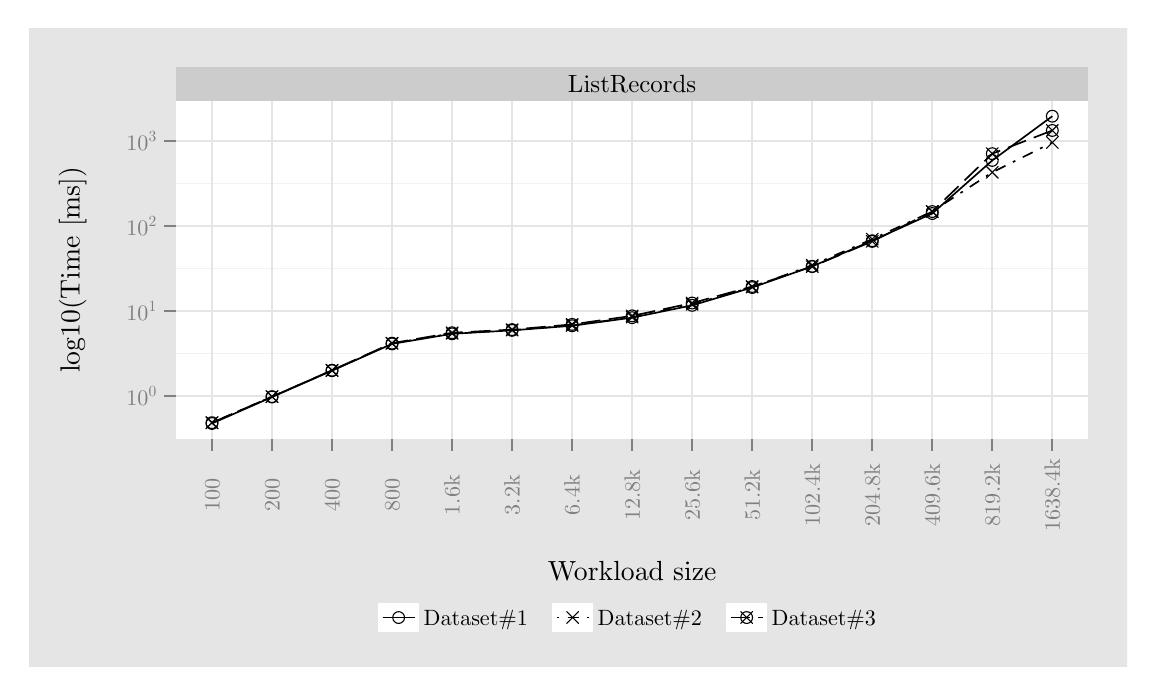
\begin{tikzpicture}[x=1pt,y=1pt]
\definecolor[named]{fillColor}{rgb}{1.00,1.00,1.00}
\path[use as bounding box,fill=fillColor,fill opacity=0.00] (0,0) rectangle (397.48,231.26);
\begin{scope}
\path[clip] (  0.00,  0.00) rectangle (397.48,231.26);
\definecolor[named]{drawColor}{rgb}{1.00,1.00,1.00}
\definecolor[named]{fillColor}{rgb}{0.90,0.90,0.90}

\path[draw=drawColor,line width= 0.6pt,line join=round,line cap=round,fill=fillColor] (  0.00,  0.00) rectangle (397.48,231.26);
\end{scope}
\begin{scope}
\path[clip] ( 53.58, 82.69) rectangle (383.26,204.82);
\definecolor[named]{fillColor}{rgb}{1.00,1.00,1.00}

\path[fill=fillColor] ( 53.58, 82.69) rectangle (383.26,204.82);
\definecolor[named]{drawColor}{rgb}{0.95,0.95,0.95}

\path[draw=drawColor,line width= 0.3pt,line join=round] ( 53.58,113.45) --
	(383.26,113.45);

\path[draw=drawColor,line width= 0.3pt,line join=round] ( 53.58,144.24) --
	(383.26,144.24);

\path[draw=drawColor,line width= 0.3pt,line join=round] ( 53.58,175.03) --
	(383.26,175.03);
\definecolor[named]{drawColor}{rgb}{0.90,0.90,0.90}

\path[draw=drawColor,line width= 0.6pt,line join=round] ( 53.58, 98.06) --
	(383.26, 98.06);

\path[draw=drawColor,line width= 0.6pt,line join=round] ( 53.58,128.85) --
	(383.26,128.85);

\path[draw=drawColor,line width= 0.6pt,line join=round] ( 53.58,159.64) --
	(383.26,159.64);

\path[draw=drawColor,line width= 0.6pt,line join=round] ( 53.58,190.42) --
	(383.26,190.42);

\path[draw=drawColor,line width= 0.6pt,line join=round] ( 66.60, 82.69) --
	( 66.60,204.82);

\path[draw=drawColor,line width= 0.6pt,line join=round] ( 88.29, 82.69) --
	( 88.29,204.82);

\path[draw=drawColor,line width= 0.6pt,line join=round] (109.97, 82.69) --
	(109.97,204.82);

\path[draw=drawColor,line width= 0.6pt,line join=round] (131.66, 82.69) --
	(131.66,204.82);

\path[draw=drawColor,line width= 0.6pt,line join=round] (153.35, 82.69) --
	(153.35,204.82);

\path[draw=drawColor,line width= 0.6pt,line join=round] (175.04, 82.69) --
	(175.04,204.82);

\path[draw=drawColor,line width= 0.6pt,line join=round] (196.73, 82.69) --
	(196.73,204.82);

\path[draw=drawColor,line width= 0.6pt,line join=round] (218.42, 82.69) --
	(218.42,204.82);

\path[draw=drawColor,line width= 0.6pt,line join=round] (240.11, 82.69) --
	(240.11,204.82);

\path[draw=drawColor,line width= 0.6pt,line join=round] (261.80, 82.69) --
	(261.80,204.82);

\path[draw=drawColor,line width= 0.6pt,line join=round] (283.49, 82.69) --
	(283.49,204.82);

\path[draw=drawColor,line width= 0.6pt,line join=round] (305.18, 82.69) --
	(305.18,204.82);

\path[draw=drawColor,line width= 0.6pt,line join=round] (326.87, 82.69) --
	(326.87,204.82);

\path[draw=drawColor,line width= 0.6pt,line join=round] (348.56, 82.69) --
	(348.56,204.82);

\path[draw=drawColor,line width= 0.6pt,line join=round] (370.25, 82.69) --
	(370.25,204.82);
\definecolor[named]{drawColor}{rgb}{0.00,0.00,0.00}

\path[draw=drawColor,line width= 0.6pt,line join=round] ( 66.60, 88.24) --
	( 88.29, 97.79) --
	(109.97,107.32) --
	(131.66,116.99) --
	(153.35,120.63) --
	(175.04,121.88) --
	(196.73,123.55) --
	(218.42,126.47) --
	(240.11,130.92) --
	(261.80,137.36) --
	(283.49,145.00) --
	(305.18,154.27) --
	(326.87,164.11) --
	(348.56,183.29) --
	(370.25,199.27);

\path[draw=drawColor,line width= 0.6pt,dash pattern=on 1pt off 3pt on 4pt off 3pt ,line join=round] ( 66.60, 88.52) --
	( 88.29, 97.92) --
	(109.97,107.39) --
	(131.66,117.15) --
	(153.35,120.78) --
	(175.04,121.95) --
	(196.73,123.65) --
	(218.42,126.66) --
	(240.11,131.25) --
	(261.80,137.50) --
	(283.49,145.46) --
	(305.18,154.83) --
	(326.87,164.86) --
	(348.56,179.00) --
	(370.25,189.76);

\path[draw=drawColor,line width= 0.6pt,dash pattern=on 7pt off 3pt ,line join=round] ( 66.60, 88.52) --
	( 88.29, 97.92) --
	(109.97,107.46) --
	(131.66,117.25) --
	(153.35,121.02) --
	(175.04,122.15) --
	(196.73,124.04) --
	(218.42,127.12) --
	(240.11,131.75) --
	(261.80,137.73) --
	(283.49,144.94) --
	(305.18,154.03) --
	(326.87,164.81) --
	(348.56,185.73) --
	(370.25,194.11);

\path[draw=drawColor,line width= 0.4pt,line join=round,line cap=round] ( 66.60, 88.24) circle (  2.13);

\path[draw=drawColor,line width= 0.4pt,line join=round,line cap=round] ( 88.29, 97.79) circle (  2.13);

\path[draw=drawColor,line width= 0.4pt,line join=round,line cap=round] (109.97,107.32) circle (  2.13);

\path[draw=drawColor,line width= 0.4pt,line join=round,line cap=round] (131.66,116.99) circle (  2.13);

\path[draw=drawColor,line width= 0.4pt,line join=round,line cap=round] (153.35,120.63) circle (  2.13);

\path[draw=drawColor,line width= 0.4pt,line join=round,line cap=round] (175.04,121.88) circle (  2.13);

\path[draw=drawColor,line width= 0.4pt,line join=round,line cap=round] (196.73,123.55) circle (  2.13);

\path[draw=drawColor,line width= 0.4pt,line join=round,line cap=round] (218.42,126.47) circle (  2.13);

\path[draw=drawColor,line width= 0.4pt,line join=round,line cap=round] (240.11,130.92) circle (  2.13);

\path[draw=drawColor,line width= 0.4pt,line join=round,line cap=round] (261.80,137.36) circle (  2.13);

\path[draw=drawColor,line width= 0.4pt,line join=round,line cap=round] (283.49,145.00) circle (  2.13);

\path[draw=drawColor,line width= 0.4pt,line join=round,line cap=round] (305.18,154.27) circle (  2.13);

\path[draw=drawColor,line width= 0.4pt,line join=round,line cap=round] (326.87,164.11) circle (  2.13);

\path[draw=drawColor,line width= 0.4pt,line join=round,line cap=round] (348.56,183.29) circle (  2.13);

\path[draw=drawColor,line width= 0.4pt,line join=round,line cap=round] (370.25,199.27) circle (  2.13);

\path[draw=drawColor,line width= 0.4pt,line join=round,line cap=round] ( 66.60, 88.52) circle (  2.13);

\path[draw=drawColor,line width= 0.4pt,line join=round,line cap=round] ( 64.46, 86.38) -- ( 68.73, 90.65);

\path[draw=drawColor,line width= 0.4pt,line join=round,line cap=round] ( 64.46, 90.65) -- ( 68.73, 86.38);

\path[draw=drawColor,line width= 0.4pt,line join=round,line cap=round] ( 88.29, 97.92) circle (  2.13);

\path[draw=drawColor,line width= 0.4pt,line join=round,line cap=round] ( 86.15, 95.79) -- ( 90.42,100.06);

\path[draw=drawColor,line width= 0.4pt,line join=round,line cap=round] ( 86.15,100.06) -- ( 90.42, 95.79);

\path[draw=drawColor,line width= 0.4pt,line join=round,line cap=round] (109.97,107.46) circle (  2.13);

\path[draw=drawColor,line width= 0.4pt,line join=round,line cap=round] (107.84,105.32) -- (112.11,109.59);

\path[draw=drawColor,line width= 0.4pt,line join=round,line cap=round] (107.84,109.59) -- (112.11,105.32);

\path[draw=drawColor,line width= 0.4pt,line join=round,line cap=round] (131.66,117.25) circle (  2.13);

\path[draw=drawColor,line width= 0.4pt,line join=round,line cap=round] (129.53,115.11) -- (133.80,119.38);

\path[draw=drawColor,line width= 0.4pt,line join=round,line cap=round] (129.53,119.38) -- (133.80,115.11);

\path[draw=drawColor,line width= 0.4pt,line join=round,line cap=round] (153.35,121.02) circle (  2.13);

\path[draw=drawColor,line width= 0.4pt,line join=round,line cap=round] (151.22,118.89) -- (155.49,123.15);

\path[draw=drawColor,line width= 0.4pt,line join=round,line cap=round] (151.22,123.15) -- (155.49,118.89);

\path[draw=drawColor,line width= 0.4pt,line join=round,line cap=round] (175.04,122.15) circle (  2.13);

\path[draw=drawColor,line width= 0.4pt,line join=round,line cap=round] (172.91,120.01) -- (177.18,124.28);

\path[draw=drawColor,line width= 0.4pt,line join=round,line cap=round] (172.91,124.28) -- (177.18,120.01);

\path[draw=drawColor,line width= 0.4pt,line join=round,line cap=round] (196.73,124.04) circle (  2.13);

\path[draw=drawColor,line width= 0.4pt,line join=round,line cap=round] (194.60,121.90) -- (198.87,126.17);

\path[draw=drawColor,line width= 0.4pt,line join=round,line cap=round] (194.60,126.17) -- (198.87,121.90);

\path[draw=drawColor,line width= 0.4pt,line join=round,line cap=round] (218.42,127.12) circle (  2.13);

\path[draw=drawColor,line width= 0.4pt,line join=round,line cap=round] (216.29,124.99) -- (220.55,129.26);

\path[draw=drawColor,line width= 0.4pt,line join=round,line cap=round] (216.29,129.26) -- (220.55,124.99);

\path[draw=drawColor,line width= 0.4pt,line join=round,line cap=round] (240.11,131.75) circle (  2.13);

\path[draw=drawColor,line width= 0.4pt,line join=round,line cap=round] (237.98,129.62) -- (242.24,133.89);

\path[draw=drawColor,line width= 0.4pt,line join=round,line cap=round] (237.98,133.89) -- (242.24,129.62);

\path[draw=drawColor,line width= 0.4pt,line join=round,line cap=round] (261.80,137.73) circle (  2.13);

\path[draw=drawColor,line width= 0.4pt,line join=round,line cap=round] (259.67,135.59) -- (263.93,139.86);

\path[draw=drawColor,line width= 0.4pt,line join=round,line cap=round] (259.67,139.86) -- (263.93,135.59);

\path[draw=drawColor,line width= 0.4pt,line join=round,line cap=round] (283.49,144.94) circle (  2.13);

\path[draw=drawColor,line width= 0.4pt,line join=round,line cap=round] (281.35,142.80) -- (285.62,147.07);

\path[draw=drawColor,line width= 0.4pt,line join=round,line cap=round] (281.35,147.07) -- (285.62,142.80);

\path[draw=drawColor,line width= 0.4pt,line join=round,line cap=round] (305.18,154.03) circle (  2.13);

\path[draw=drawColor,line width= 0.4pt,line join=round,line cap=round] (303.04,151.90) -- (307.31,156.17);

\path[draw=drawColor,line width= 0.4pt,line join=round,line cap=round] (303.04,156.17) -- (307.31,151.90);

\path[draw=drawColor,line width= 0.4pt,line join=round,line cap=round] (326.87,164.81) circle (  2.13);

\path[draw=drawColor,line width= 0.4pt,line join=round,line cap=round] (324.73,162.67) -- (329.00,166.94);

\path[draw=drawColor,line width= 0.4pt,line join=round,line cap=round] (324.73,166.94) -- (329.00,162.67);

\path[draw=drawColor,line width= 0.4pt,line join=round,line cap=round] (348.56,185.73) circle (  2.13);

\path[draw=drawColor,line width= 0.4pt,line join=round,line cap=round] (346.42,183.60) -- (350.69,187.87);

\path[draw=drawColor,line width= 0.4pt,line join=round,line cap=round] (346.42,187.87) -- (350.69,183.60);

\path[draw=drawColor,line width= 0.4pt,line join=round,line cap=round] (370.25,194.11) circle (  2.13);

\path[draw=drawColor,line width= 0.4pt,line join=round,line cap=round] (368.11,191.98) -- (372.38,196.25);

\path[draw=drawColor,line width= 0.4pt,line join=round,line cap=round] (368.11,196.25) -- (372.38,191.98);

\path[draw=drawColor,line width= 0.4pt,line join=round,line cap=round,fill=fillColor] ( 64.46, 86.38) -- ( 68.73, 90.65);

\path[draw=drawColor,line width= 0.4pt,line join=round,line cap=round,fill=fillColor] ( 64.46, 90.65) -- ( 68.73, 86.38);

\path[draw=drawColor,line width= 0.4pt,line join=round,line cap=round,fill=fillColor] ( 86.15, 95.79) -- ( 90.42,100.06);

\path[draw=drawColor,line width= 0.4pt,line join=round,line cap=round,fill=fillColor] ( 86.15,100.06) -- ( 90.42, 95.79);

\path[draw=drawColor,line width= 0.4pt,line join=round,line cap=round,fill=fillColor] (107.84,105.26) -- (112.11,109.53);

\path[draw=drawColor,line width= 0.4pt,line join=round,line cap=round,fill=fillColor] (107.84,109.53) -- (112.11,105.26);

\path[draw=drawColor,line width= 0.4pt,line join=round,line cap=round,fill=fillColor] (129.53,115.02) -- (133.80,119.28);

\path[draw=drawColor,line width= 0.4pt,line join=round,line cap=round,fill=fillColor] (129.53,119.28) -- (133.80,115.02);

\path[draw=drawColor,line width= 0.4pt,line join=round,line cap=round,fill=fillColor] (151.22,118.64) -- (155.49,122.91);

\path[draw=drawColor,line width= 0.4pt,line join=round,line cap=round,fill=fillColor] (151.22,122.91) -- (155.49,118.64);

\path[draw=drawColor,line width= 0.4pt,line join=round,line cap=round,fill=fillColor] (172.91,119.81) -- (177.18,124.08);

\path[draw=drawColor,line width= 0.4pt,line join=round,line cap=round,fill=fillColor] (172.91,124.08) -- (177.18,119.81);

\path[draw=drawColor,line width= 0.4pt,line join=round,line cap=round,fill=fillColor] (194.60,121.52) -- (198.87,125.78);

\path[draw=drawColor,line width= 0.4pt,line join=round,line cap=round,fill=fillColor] (194.60,125.78) -- (198.87,121.52);

\path[draw=drawColor,line width= 0.4pt,line join=round,line cap=round,fill=fillColor] (216.29,124.52) -- (220.55,128.79);

\path[draw=drawColor,line width= 0.4pt,line join=round,line cap=round,fill=fillColor] (216.29,128.79) -- (220.55,124.52);

\path[draw=drawColor,line width= 0.4pt,line join=round,line cap=round,fill=fillColor] (237.98,129.12) -- (242.24,133.38);

\path[draw=drawColor,line width= 0.4pt,line join=round,line cap=round,fill=fillColor] (237.98,133.38) -- (242.24,129.12);

\path[draw=drawColor,line width= 0.4pt,line join=round,line cap=round,fill=fillColor] (259.67,135.36) -- (263.93,139.63);

\path[draw=drawColor,line width= 0.4pt,line join=round,line cap=round,fill=fillColor] (259.67,139.63) -- (263.93,135.36);

\path[draw=drawColor,line width= 0.4pt,line join=round,line cap=round,fill=fillColor] (281.35,143.32) -- (285.62,147.59);

\path[draw=drawColor,line width= 0.4pt,line join=round,line cap=round,fill=fillColor] (281.35,147.59) -- (285.62,143.32);

\path[draw=drawColor,line width= 0.4pt,line join=round,line cap=round,fill=fillColor] (303.04,152.70) -- (307.31,156.97);

\path[draw=drawColor,line width= 0.4pt,line join=round,line cap=round,fill=fillColor] (303.04,156.97) -- (307.31,152.70);

\path[draw=drawColor,line width= 0.4pt,line join=round,line cap=round,fill=fillColor] (324.73,162.73) -- (329.00,167.00);

\path[draw=drawColor,line width= 0.4pt,line join=round,line cap=round,fill=fillColor] (324.73,167.00) -- (329.00,162.73);

\path[draw=drawColor,line width= 0.4pt,line join=round,line cap=round,fill=fillColor] (346.42,176.87) -- (350.69,181.13);

\path[draw=drawColor,line width= 0.4pt,line join=round,line cap=round,fill=fillColor] (346.42,181.13) -- (350.69,176.87);

\path[draw=drawColor,line width= 0.4pt,line join=round,line cap=round,fill=fillColor] (368.11,187.63) -- (372.38,191.90);

\path[draw=drawColor,line width= 0.4pt,line join=round,line cap=round,fill=fillColor] (368.11,191.90) -- (372.38,187.63);
\end{scope}
\begin{scope}
\path[clip] (  0.00,  0.00) rectangle (397.48,231.26);
\definecolor[named]{fillColor}{rgb}{0.80,0.80,0.80}

\path[fill=fillColor] ( 53.58,204.82) rectangle (383.26,217.04);
\definecolor[named]{drawColor}{rgb}{0.00,0.00,0.00}

\node[text=drawColor,anchor=base,inner sep=0pt, outer sep=0pt, scale=  0.90] at (218.42,207.83) {ListRecords};
\end{scope}
\begin{scope}
\path[clip] (  0.00,  0.00) rectangle (397.48,231.26);
\definecolor[named]{drawColor}{rgb}{0.50,0.50,0.50}

\node[text=drawColor,anchor=base west,inner sep=0pt, outer sep=0pt, scale=  0.80] at ( 35.67, 94.62) {10};

\node[text=drawColor,anchor=base west,inner sep=0pt, outer sep=0pt, scale=  0.56] at ( 43.67, 97.90) {0};

\node[text=drawColor,anchor=base west,inner sep=0pt, outer sep=0pt, scale=  0.80] at ( 35.67,125.41) {10};

\node[text=drawColor,anchor=base west,inner sep=0pt, outer sep=0pt, scale=  0.56] at ( 43.67,128.69) {1};

\node[text=drawColor,anchor=base west,inner sep=0pt, outer sep=0pt, scale=  0.80] at ( 35.67,156.20) {10};

\node[text=drawColor,anchor=base west,inner sep=0pt, outer sep=0pt, scale=  0.56] at ( 43.67,159.47) {2};

\node[text=drawColor,anchor=base west,inner sep=0pt, outer sep=0pt, scale=  0.80] at ( 35.67,186.99) {10};

\node[text=drawColor,anchor=base west,inner sep=0pt, outer sep=0pt, scale=  0.56] at ( 43.67,190.26) {3};
\end{scope}
\begin{scope}
\path[clip] (  0.00,  0.00) rectangle (397.48,231.26);
\definecolor[named]{drawColor}{rgb}{0.50,0.50,0.50}

\path[draw=drawColor,line width= 0.6pt,line join=round] ( 49.31, 98.06) --
	( 53.58, 98.06);

\path[draw=drawColor,line width= 0.6pt,line join=round] ( 49.31,128.85) --
	( 53.58,128.85);

\path[draw=drawColor,line width= 0.6pt,line join=round] ( 49.31,159.64) --
	( 53.58,159.64);

\path[draw=drawColor,line width= 0.6pt,line join=round] ( 49.31,190.42) --
	( 53.58,190.42);
\end{scope}
\begin{scope}
\path[clip] (  0.00,  0.00) rectangle (397.48,231.26);
\definecolor[named]{drawColor}{rgb}{0.50,0.50,0.50}

\path[draw=drawColor,line width= 0.6pt,line join=round] ( 66.60, 78.42) --
	( 66.60, 82.69);

\path[draw=drawColor,line width= 0.6pt,line join=round] ( 88.29, 78.42) --
	( 88.29, 82.69);

\path[draw=drawColor,line width= 0.6pt,line join=round] (109.97, 78.42) --
	(109.97, 82.69);

\path[draw=drawColor,line width= 0.6pt,line join=round] (131.66, 78.42) --
	(131.66, 82.69);

\path[draw=drawColor,line width= 0.6pt,line join=round] (153.35, 78.42) --
	(153.35, 82.69);

\path[draw=drawColor,line width= 0.6pt,line join=round] (175.04, 78.42) --
	(175.04, 82.69);

\path[draw=drawColor,line width= 0.6pt,line join=round] (196.73, 78.42) --
	(196.73, 82.69);

\path[draw=drawColor,line width= 0.6pt,line join=round] (218.42, 78.42) --
	(218.42, 82.69);

\path[draw=drawColor,line width= 0.6pt,line join=round] (240.11, 78.42) --
	(240.11, 82.69);

\path[draw=drawColor,line width= 0.6pt,line join=round] (261.80, 78.42) --
	(261.80, 82.69);

\path[draw=drawColor,line width= 0.6pt,line join=round] (283.49, 78.42) --
	(283.49, 82.69);

\path[draw=drawColor,line width= 0.6pt,line join=round] (305.18, 78.42) --
	(305.18, 82.69);

\path[draw=drawColor,line width= 0.6pt,line join=round] (326.87, 78.42) --
	(326.87, 82.69);

\path[draw=drawColor,line width= 0.6pt,line join=round] (348.56, 78.42) --
	(348.56, 82.69);

\path[draw=drawColor,line width= 0.6pt,line join=round] (370.25, 78.42) --
	(370.25, 82.69);
\end{scope}
\begin{scope}
\path[clip] (  0.00,  0.00) rectangle (397.48,231.26);
\definecolor[named]{drawColor}{rgb}{0.50,0.50,0.50}

\node[text=drawColor,rotate= 90.00,anchor=base,inner sep=0pt, outer sep=0pt, scale=  0.80] at ( 69.35, 62.36) {100};

\node[text=drawColor,rotate= 90.00,anchor=base,inner sep=0pt, outer sep=0pt, scale=  0.80] at ( 91.04, 62.36) {200};

\node[text=drawColor,rotate= 90.00,anchor=base,inner sep=0pt, outer sep=0pt, scale=  0.80] at (112.73, 62.36) {400};

\node[text=drawColor,rotate= 90.00,anchor=base,inner sep=0pt, outer sep=0pt, scale=  0.80] at (134.42, 62.36) {800};

\node[text=drawColor,rotate= 90.00,anchor=base,inner sep=0pt, outer sep=0pt, scale=  0.80] at (156.11, 62.36) {1.6k};

\node[text=drawColor,rotate= 90.00,anchor=base,inner sep=0pt, outer sep=0pt, scale=  0.80] at (177.80, 62.36) {3.2k};

\node[text=drawColor,rotate= 90.00,anchor=base,inner sep=0pt, outer sep=0pt, scale=  0.80] at (199.49, 62.36) {6.4k};

\node[text=drawColor,rotate= 90.00,anchor=base,inner sep=0pt, outer sep=0pt, scale=  0.80] at (221.18, 62.36) {12.8k};

\node[text=drawColor,rotate= 90.00,anchor=base,inner sep=0pt, outer sep=0pt, scale=  0.80] at (242.86, 62.36) {25.6k};

\node[text=drawColor,rotate= 90.00,anchor=base,inner sep=0pt, outer sep=0pt, scale=  0.80] at (264.55, 62.36) {51.2k};

\node[text=drawColor,rotate= 90.00,anchor=base,inner sep=0pt, outer sep=0pt, scale=  0.80] at (286.24, 62.36) {102.4k};

\node[text=drawColor,rotate= 90.00,anchor=base,inner sep=0pt, outer sep=0pt, scale=  0.80] at (307.93, 62.36) {204.8k};

\node[text=drawColor,rotate= 90.00,anchor=base,inner sep=0pt, outer sep=0pt, scale=  0.80] at (329.62, 62.36) {409.6k};

\node[text=drawColor,rotate= 90.00,anchor=base,inner sep=0pt, outer sep=0pt, scale=  0.80] at (351.31, 62.36) {819.2k};

\node[text=drawColor,rotate= 90.00,anchor=base,inner sep=0pt, outer sep=0pt, scale=  0.80] at (373.00, 62.36) {1638.4k};
\end{scope}
\begin{scope}
\path[clip] (  0.00,  0.00) rectangle (397.48,231.26);
\definecolor[named]{drawColor}{rgb}{0.00,0.00,0.00}

\node[text=drawColor,anchor=base,inner sep=0pt, outer sep=0pt, scale=  1.00] at (218.42, 31.41) {Workload size};
\end{scope}
\begin{scope}
\path[clip] (  0.00,  0.00) rectangle (397.48,231.26);
\definecolor[named]{drawColor}{rgb}{0.00,0.00,0.00}

\node[text=drawColor,rotate= 90.00,anchor=base,inner sep=0pt, outer sep=0pt, scale=  1.00] at ( 18.80,143.75) {log10(Time [ms])};
\end{scope}
\begin{scope}
\path[clip] (  0.00,  0.00) rectangle (397.48,231.26);
\definecolor[named]{fillColor}{rgb}{0.90,0.90,0.90}

\path[fill=fillColor] (118.93,  8.87) rectangle (317.91, 27.36);
\end{scope}
\begin{scope}
\path[clip] (  0.00,  0.00) rectangle (397.48,231.26);
\definecolor[named]{drawColor}{rgb}{1.00,1.00,1.00}
\definecolor[named]{fillColor}{rgb}{1.00,1.00,1.00}

\path[draw=drawColor,line width= 0.6pt,line join=round,line cap=round,fill=fillColor] (126.81, 13.14) rectangle (141.26, 23.09);
\end{scope}
\begin{scope}
\path[clip] (  0.00,  0.00) rectangle (397.48,231.26);
\definecolor[named]{drawColor}{rgb}{0.00,0.00,0.00}

\path[draw=drawColor,line width= 0.6pt,line join=round] (128.26, 18.11) -- (139.82, 18.11);
\end{scope}
\begin{scope}
\path[clip] (  0.00,  0.00) rectangle (397.48,231.26);
\definecolor[named]{drawColor}{rgb}{0.00,0.00,0.00}

\path[draw=drawColor,line width= 0.4pt,line join=round,line cap=round] (134.04, 18.11) circle (  2.13);
\end{scope}
\begin{scope}
\path[clip] (  0.00,  0.00) rectangle (397.48,231.26);
\definecolor[named]{drawColor}{rgb}{1.00,1.00,1.00}
\definecolor[named]{fillColor}{rgb}{1.00,1.00,1.00}

\path[draw=drawColor,line width= 0.6pt,line join=round,line cap=round,fill=fillColor] (189.69, 13.14) rectangle (204.14, 23.09);
\end{scope}
\begin{scope}
\path[clip] (  0.00,  0.00) rectangle (397.48,231.26);
\definecolor[named]{drawColor}{rgb}{0.00,0.00,0.00}

\path[draw=drawColor,line width= 0.6pt,dash pattern=on 1pt off 3pt on 4pt off 3pt ,line join=round] (191.14, 18.11) -- (202.70, 18.11);
\end{scope}
\begin{scope}
\path[clip] (  0.00,  0.00) rectangle (397.48,231.26);
\definecolor[named]{drawColor}{rgb}{0.00,0.00,0.00}
\definecolor[named]{fillColor}{rgb}{1.00,1.00,1.00}

\path[draw=drawColor,line width= 0.4pt,line join=round,line cap=round,fill=fillColor] (194.78, 15.98) -- (199.05, 20.25);

\path[draw=drawColor,line width= 0.4pt,line join=round,line cap=round,fill=fillColor] (194.78, 20.25) -- (199.05, 15.98);
\end{scope}
\begin{scope}
\path[clip] (  0.00,  0.00) rectangle (397.48,231.26);
\definecolor[named]{drawColor}{rgb}{1.00,1.00,1.00}
\definecolor[named]{fillColor}{rgb}{1.00,1.00,1.00}

\path[draw=drawColor,line width= 0.6pt,line join=round,line cap=round,fill=fillColor] (252.57, 13.14) rectangle (267.02, 23.09);
\end{scope}
\begin{scope}
\path[clip] (  0.00,  0.00) rectangle (397.48,231.26);
\definecolor[named]{drawColor}{rgb}{0.00,0.00,0.00}

\path[draw=drawColor,line width= 0.6pt,dash pattern=on 7pt off 3pt ,line join=round] (254.02, 18.11) -- (265.58, 18.11);
\end{scope}
\begin{scope}
\path[clip] (  0.00,  0.00) rectangle (397.48,231.26);
\definecolor[named]{drawColor}{rgb}{0.00,0.00,0.00}

\path[draw=drawColor,line width= 0.4pt,line join=round,line cap=round] (259.80, 18.11) circle (  2.13);

\path[draw=drawColor,line width= 0.4pt,line join=round,line cap=round] (257.66, 15.98) -- (261.93, 20.25);

\path[draw=drawColor,line width= 0.4pt,line join=round,line cap=round] (257.66, 20.25) -- (261.93, 15.98);
\end{scope}
\begin{scope}
\path[clip] (  0.00,  0.00) rectangle (397.48,231.26);
\definecolor[named]{drawColor}{rgb}{0.00,0.00,0.00}

\node[text=drawColor,anchor=base west,inner sep=0pt, outer sep=0pt, scale=  0.80] at (143.07, 15.36) {Dataset\#1 $\;\;$};
\end{scope}
\begin{scope}
\path[clip] (  0.00,  0.00) rectangle (397.48,231.26);
\definecolor[named]{drawColor}{rgb}{0.00,0.00,0.00}

\node[text=drawColor,anchor=base west,inner sep=0pt, outer sep=0pt, scale=  0.80] at (205.95, 15.36) {Dataset\#2 $\;\;$};
\end{scope}
\begin{scope}
\path[clip] (  0.00,  0.00) rectangle (397.48,231.26);
\definecolor[named]{drawColor}{rgb}{0.00,0.00,0.00}

\node[text=drawColor,anchor=base west,inner sep=0pt, outer sep=0pt, scale=  0.80] at (268.83, 15.36) {Dataset\#3 $\;\;$};
\end{scope}
\end{tikzpicture}

 }
 \caption[OAI-PMH data provider\index{OAI-PMH!Data Provider} ListRecords\index{OAI-PMH!Verbs!ListRecords} performance]{OAI-PMH data provider\index{OAI-PMH!Data Provider} ListRecords\index{OAI-PMH!Verbs!ListRecords} performance}
 \label{fig:experimentation:performance:oaipmh:listrecords-level}
\end{figure}

\begin{figure}
 \centering
 \framebox[\textwidth]{%
% Created by tikzDevice version 0.6.2-92-0ad2792 on 2013-03-23 23:05:55
% !TEX encoding = UTF-8 Unicode
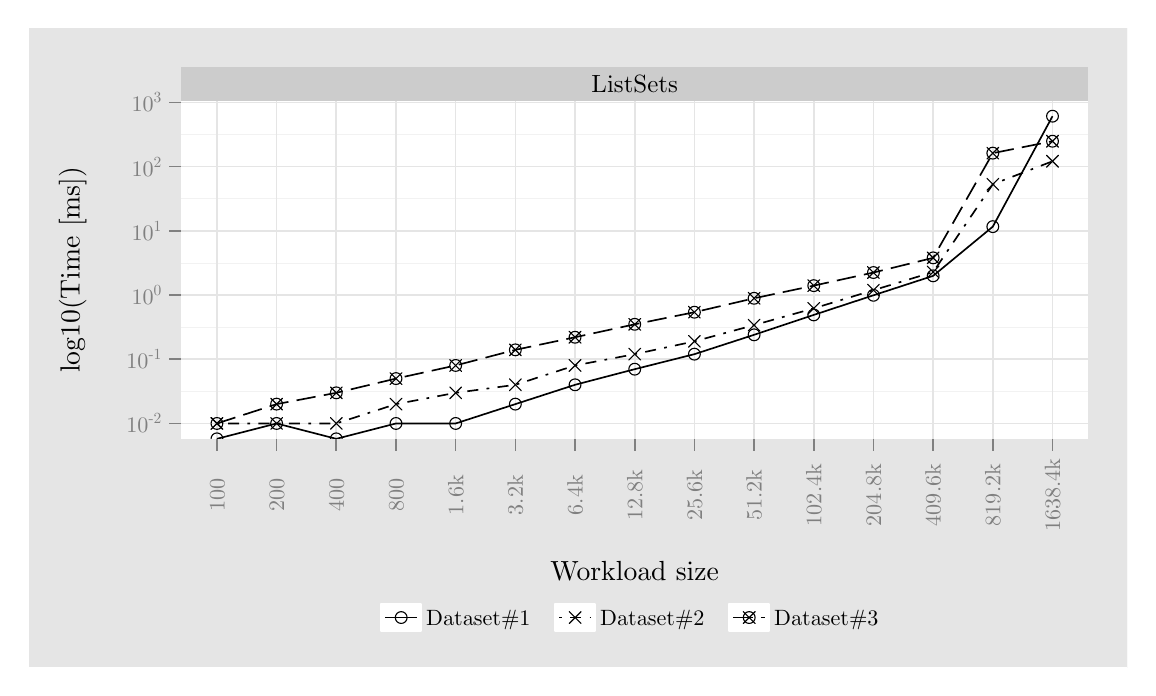
\begin{tikzpicture}[x=1pt,y=1pt]
\definecolor[named]{fillColor}{rgb}{1.00,1.00,1.00}
\path[use as bounding box,fill=fillColor,fill opacity=0.00] (0,0) rectangle (397.48,231.26);
\begin{scope}
\path[clip] (  0.00,  0.00) rectangle (397.48,231.26);
\definecolor[named]{drawColor}{rgb}{1.00,1.00,1.00}
\definecolor[named]{fillColor}{rgb}{0.90,0.90,0.90}

\path[draw=drawColor,line width= 0.6pt,line join=round,line cap=round,fill=fillColor] (  0.00,  0.00) rectangle (397.48,231.26);
\end{scope}
\begin{scope}
\path[clip] ( 55.45, 82.69) rectangle (383.26,204.82);
\definecolor[named]{fillColor}{rgb}{1.00,1.00,1.00}

\path[fill=fillColor] ( 55.45, 82.69) rectangle (383.26,204.82);
\definecolor[named]{drawColor}{rgb}{0.95,0.95,0.95}

\path[draw=drawColor,line width= 0.3pt,line join=round] ( 55.45, 99.84) --
	(383.26, 99.84);

\path[draw=drawColor,line width= 0.3pt,line join=round] ( 55.45,123.05) --
	(383.26,123.05);

\path[draw=drawColor,line width= 0.3pt,line join=round] ( 55.45,146.25) --
	(383.26,146.25);

\path[draw=drawColor,line width= 0.3pt,line join=round] ( 55.45,169.45) --
	(383.26,169.45);

\path[draw=drawColor,line width= 0.3pt,line join=round] ( 55.45,192.66) --
	(383.26,192.66);
\definecolor[named]{drawColor}{rgb}{0.90,0.90,0.90}

\path[draw=drawColor,line width= 0.6pt,line join=round] ( 55.45, 88.24) --
	(383.26, 88.24);

\path[draw=drawColor,line width= 0.6pt,line join=round] ( 55.45,111.45) --
	(383.26,111.45);

\path[draw=drawColor,line width= 0.6pt,line join=round] ( 55.45,134.65) --
	(383.26,134.65);

\path[draw=drawColor,line width= 0.6pt,line join=round] ( 55.45,157.85) --
	(383.26,157.85);

\path[draw=drawColor,line width= 0.6pt,line join=round] ( 55.45,181.06) --
	(383.26,181.06);

\path[draw=drawColor,line width= 0.6pt,line join=round] ( 55.45,204.26) --
	(383.26,204.26);

\path[draw=drawColor,line width= 0.6pt,line join=round] ( 68.39, 82.69) --
	( 68.39,204.82);

\path[draw=drawColor,line width= 0.6pt,line join=round] ( 89.95, 82.69) --
	( 89.95,204.82);

\path[draw=drawColor,line width= 0.6pt,line join=round] (111.52, 82.69) --
	(111.52,204.82);

\path[draw=drawColor,line width= 0.6pt,line join=round] (133.09, 82.69) --
	(133.09,204.82);

\path[draw=drawColor,line width= 0.6pt,line join=round] (154.65, 82.69) --
	(154.65,204.82);

\path[draw=drawColor,line width= 0.6pt,line join=round] (176.22, 82.69) --
	(176.22,204.82);

\path[draw=drawColor,line width= 0.6pt,line join=round] (197.79, 82.69) --
	(197.79,204.82);

\path[draw=drawColor,line width= 0.6pt,line join=round] (219.35, 82.69) --
	(219.35,204.82);

\path[draw=drawColor,line width= 0.6pt,line join=round] (240.92, 82.69) --
	(240.92,204.82);

\path[draw=drawColor,line width= 0.6pt,line join=round] (262.49, 82.69) --
	(262.49,204.82);

\path[draw=drawColor,line width= 0.6pt,line join=round] (284.05, 82.69) --
	(284.05,204.82);

\path[draw=drawColor,line width= 0.6pt,line join=round] (305.62, 82.69) --
	(305.62,204.82);

\path[draw=drawColor,line width= 0.6pt,line join=round] (327.19, 82.69) --
	(327.19,204.82);

\path[draw=drawColor,line width= 0.6pt,line join=round] (348.75, 82.69) --
	(348.75,204.82);

\path[draw=drawColor,line width= 0.6pt,line join=round] (370.32, 82.69) --
	(370.32,204.82);
\definecolor[named]{drawColor}{rgb}{0.00,0.00,0.00}

\path[draw=drawColor,line width= 0.6pt,line join=round] ( 68.39, 82.69) --
	( 89.95, 88.24) --
	(111.52, 82.69) --
	(133.09, 88.24) --
	(154.65, 88.24) --
	(176.22, 95.23) --
	(197.79,102.21) --
	(219.35,107.85) --
	(240.92,113.28) --
	(262.49,120.27) --
	(284.05,127.46) --
	(305.62,134.55) --
	(327.19,141.58) --
	(348.75,159.36) --
	(370.32,199.27);

\path[draw=drawColor,line width= 0.6pt,dash pattern=on 1pt off 3pt on 4pt off 3pt ,line join=round] ( 68.39, 88.24) --
	( 89.95, 88.24) --
	(111.52, 88.24) --
	(133.09, 95.23) --
	(154.65, 99.31) --
	(176.22,102.21) --
	(197.79,109.20) --
	(219.35,113.28) --
	(240.92,117.91) --
	(262.49,123.78) --
	(284.05,129.83) --
	(305.62,136.40) --
	(327.19,142.95) --
	(348.75,174.68) --
	(370.32,182.98);

\path[draw=drawColor,line width= 0.6pt,dash pattern=on 7pt off 3pt ,line join=round] ( 68.39, 88.24) --
	( 89.95, 95.23) --
	(111.52, 99.31) --
	(133.09,104.46) --
	(154.65,109.20) --
	(176.22,114.84) --
	(197.79,119.39) --
	(219.35,124.07) --
	(240.92,128.44) --
	(262.49,133.47) --
	(284.05,138.04) --
	(305.62,142.78) --
	(327.19,148.08) --
	(348.75,185.92) --
	(370.32,190.22);

\path[draw=drawColor,line width= 0.4pt,line join=round,line cap=round] ( 68.39, 82.69) circle (  2.13);

\path[draw=drawColor,line width= 0.4pt,line join=round,line cap=round] ( 89.95, 88.24) circle (  2.13);

\path[draw=drawColor,line width= 0.4pt,line join=round,line cap=round] (111.52, 82.69) circle (  2.13);

\path[draw=drawColor,line width= 0.4pt,line join=round,line cap=round] (133.09, 88.24) circle (  2.13);

\path[draw=drawColor,line width= 0.4pt,line join=round,line cap=round] (154.65, 88.24) circle (  2.13);

\path[draw=drawColor,line width= 0.4pt,line join=round,line cap=round] (176.22, 95.23) circle (  2.13);

\path[draw=drawColor,line width= 0.4pt,line join=round,line cap=round] (197.79,102.21) circle (  2.13);

\path[draw=drawColor,line width= 0.4pt,line join=round,line cap=round] (219.35,107.85) circle (  2.13);

\path[draw=drawColor,line width= 0.4pt,line join=round,line cap=round] (240.92,113.28) circle (  2.13);

\path[draw=drawColor,line width= 0.4pt,line join=round,line cap=round] (262.49,120.27) circle (  2.13);

\path[draw=drawColor,line width= 0.4pt,line join=round,line cap=round] (284.05,127.46) circle (  2.13);

\path[draw=drawColor,line width= 0.4pt,line join=round,line cap=round] (305.62,134.55) circle (  2.13);

\path[draw=drawColor,line width= 0.4pt,line join=round,line cap=round] (327.19,141.58) circle (  2.13);

\path[draw=drawColor,line width= 0.4pt,line join=round,line cap=round] (348.75,159.36) circle (  2.13);

\path[draw=drawColor,line width= 0.4pt,line join=round,line cap=round] (370.32,199.27) circle (  2.13);

\path[draw=drawColor,line width= 0.4pt,line join=round,line cap=round] ( 68.39, 88.24) circle (  2.13);

\path[draw=drawColor,line width= 0.4pt,line join=round,line cap=round] ( 66.25, 86.11) -- ( 70.52, 90.38);

\path[draw=drawColor,line width= 0.4pt,line join=round,line cap=round] ( 66.25, 90.38) -- ( 70.52, 86.11);

\path[draw=drawColor,line width= 0.4pt,line join=round,line cap=round] ( 89.95, 95.23) circle (  2.13);

\path[draw=drawColor,line width= 0.4pt,line join=round,line cap=round] ( 87.82, 93.09) -- ( 92.09, 97.36);

\path[draw=drawColor,line width= 0.4pt,line join=round,line cap=round] ( 87.82, 97.36) -- ( 92.09, 93.09);

\path[draw=drawColor,line width= 0.4pt,line join=round,line cap=round] (111.52, 99.31) circle (  2.13);

\path[draw=drawColor,line width= 0.4pt,line join=round,line cap=round] (109.39, 97.18) -- (113.66,101.45);

\path[draw=drawColor,line width= 0.4pt,line join=round,line cap=round] (109.39,101.45) -- (113.66, 97.18);

\path[draw=drawColor,line width= 0.4pt,line join=round,line cap=round] (133.09,104.46) circle (  2.13);

\path[draw=drawColor,line width= 0.4pt,line join=round,line cap=round] (130.95,102.33) -- (135.22,106.59);

\path[draw=drawColor,line width= 0.4pt,line join=round,line cap=round] (130.95,106.59) -- (135.22,102.33);

\path[draw=drawColor,line width= 0.4pt,line join=round,line cap=round] (154.65,109.20) circle (  2.13);

\path[draw=drawColor,line width= 0.4pt,line join=round,line cap=round] (152.52,107.06) -- (156.79,111.33);

\path[draw=drawColor,line width= 0.4pt,line join=round,line cap=round] (152.52,111.33) -- (156.79,107.06);

\path[draw=drawColor,line width= 0.4pt,line join=round,line cap=round] (176.22,114.84) circle (  2.13);

\path[draw=drawColor,line width= 0.4pt,line join=round,line cap=round] (174.09,112.70) -- (178.35,116.97);

\path[draw=drawColor,line width= 0.4pt,line join=round,line cap=round] (174.09,116.97) -- (178.35,112.70);

\path[draw=drawColor,line width= 0.4pt,line join=round,line cap=round] (197.79,119.39) circle (  2.13);

\path[draw=drawColor,line width= 0.4pt,line join=round,line cap=round] (195.65,117.26) -- (199.92,121.53);

\path[draw=drawColor,line width= 0.4pt,line join=round,line cap=round] (195.65,121.53) -- (199.92,117.26);

\path[draw=drawColor,line width= 0.4pt,line join=round,line cap=round] (219.35,124.07) circle (  2.13);

\path[draw=drawColor,line width= 0.4pt,line join=round,line cap=round] (217.22,121.94) -- (221.49,126.20);

\path[draw=drawColor,line width= 0.4pt,line join=round,line cap=round] (217.22,126.20) -- (221.49,121.94);

\path[draw=drawColor,line width= 0.4pt,line join=round,line cap=round] (240.92,128.44) circle (  2.13);

\path[draw=drawColor,line width= 0.4pt,line join=round,line cap=round] (238.79,126.31) -- (243.05,130.57);

\path[draw=drawColor,line width= 0.4pt,line join=round,line cap=round] (238.79,130.57) -- (243.05,126.31);

\path[draw=drawColor,line width= 0.4pt,line join=round,line cap=round] (262.49,133.47) circle (  2.13);

\path[draw=drawColor,line width= 0.4pt,line join=round,line cap=round] (260.35,131.34) -- (264.62,135.61);

\path[draw=drawColor,line width= 0.4pt,line join=round,line cap=round] (260.35,135.61) -- (264.62,131.34);

\path[draw=drawColor,line width= 0.4pt,line join=round,line cap=round] (284.05,138.04) circle (  2.13);

\path[draw=drawColor,line width= 0.4pt,line join=round,line cap=round] (281.92,135.91) -- (286.19,140.17);

\path[draw=drawColor,line width= 0.4pt,line join=round,line cap=round] (281.92,140.17) -- (286.19,135.91);

\path[draw=drawColor,line width= 0.4pt,line join=round,line cap=round] (305.62,142.78) circle (  2.13);

\path[draw=drawColor,line width= 0.4pt,line join=round,line cap=round] (303.49,140.64) -- (307.75,144.91);

\path[draw=drawColor,line width= 0.4pt,line join=round,line cap=round] (303.49,144.91) -- (307.75,140.64);

\path[draw=drawColor,line width= 0.4pt,line join=round,line cap=round] (327.19,148.08) circle (  2.13);

\path[draw=drawColor,line width= 0.4pt,line join=round,line cap=round] (325.05,145.94) -- (329.32,150.21);

\path[draw=drawColor,line width= 0.4pt,line join=round,line cap=round] (325.05,150.21) -- (329.32,145.94);

\path[draw=drawColor,line width= 0.4pt,line join=round,line cap=round] (348.75,185.92) circle (  2.13);

\path[draw=drawColor,line width= 0.4pt,line join=round,line cap=round] (346.62,183.78) -- (350.89,188.05);

\path[draw=drawColor,line width= 0.4pt,line join=round,line cap=round] (346.62,188.05) -- (350.89,183.78);

\path[draw=drawColor,line width= 0.4pt,line join=round,line cap=round] (370.32,190.22) circle (  2.13);

\path[draw=drawColor,line width= 0.4pt,line join=round,line cap=round] (368.18,188.09) -- (372.45,192.35);

\path[draw=drawColor,line width= 0.4pt,line join=round,line cap=round] (368.18,192.35) -- (372.45,188.09);

\path[draw=drawColor,line width= 0.4pt,line join=round,line cap=round,fill=fillColor] ( 66.25, 86.11) -- ( 70.52, 90.38);

\path[draw=drawColor,line width= 0.4pt,line join=round,line cap=round,fill=fillColor] ( 66.25, 90.38) -- ( 70.52, 86.11);

\path[draw=drawColor,line width= 0.4pt,line join=round,line cap=round,fill=fillColor] ( 87.82, 86.11) -- ( 92.09, 90.38);

\path[draw=drawColor,line width= 0.4pt,line join=round,line cap=round,fill=fillColor] ( 87.82, 90.38) -- ( 92.09, 86.11);

\path[draw=drawColor,line width= 0.4pt,line join=round,line cap=round,fill=fillColor] (109.39, 86.11) -- (113.66, 90.38);

\path[draw=drawColor,line width= 0.4pt,line join=round,line cap=round,fill=fillColor] (109.39, 90.38) -- (113.66, 86.11);

\path[draw=drawColor,line width= 0.4pt,line join=round,line cap=round,fill=fillColor] (130.95, 93.09) -- (135.22, 97.36);

\path[draw=drawColor,line width= 0.4pt,line join=round,line cap=round,fill=fillColor] (130.95, 97.36) -- (135.22, 93.09);

\path[draw=drawColor,line width= 0.4pt,line join=round,line cap=round,fill=fillColor] (152.52, 97.18) -- (156.79,101.45);

\path[draw=drawColor,line width= 0.4pt,line join=round,line cap=round,fill=fillColor] (152.52,101.45) -- (156.79, 97.18);

\path[draw=drawColor,line width= 0.4pt,line join=round,line cap=round,fill=fillColor] (174.09,100.08) -- (178.35,104.35);

\path[draw=drawColor,line width= 0.4pt,line join=round,line cap=round,fill=fillColor] (174.09,104.35) -- (178.35,100.08);

\path[draw=drawColor,line width= 0.4pt,line join=round,line cap=round,fill=fillColor] (195.65,107.06) -- (199.92,111.33);

\path[draw=drawColor,line width= 0.4pt,line join=round,line cap=round,fill=fillColor] (195.65,111.33) -- (199.92,107.06);

\path[draw=drawColor,line width= 0.4pt,line join=round,line cap=round,fill=fillColor] (217.22,111.15) -- (221.49,115.42);

\path[draw=drawColor,line width= 0.4pt,line join=round,line cap=round,fill=fillColor] (217.22,115.42) -- (221.49,111.15);

\path[draw=drawColor,line width= 0.4pt,line join=round,line cap=round,fill=fillColor] (238.79,115.78) -- (243.05,120.05);

\path[draw=drawColor,line width= 0.4pt,line join=round,line cap=round,fill=fillColor] (238.79,120.05) -- (243.05,115.78);

\path[draw=drawColor,line width= 0.4pt,line join=round,line cap=round,fill=fillColor] (260.35,121.64) -- (264.62,125.91);

\path[draw=drawColor,line width= 0.4pt,line join=round,line cap=round,fill=fillColor] (260.35,125.91) -- (264.62,121.64);

\path[draw=drawColor,line width= 0.4pt,line join=round,line cap=round,fill=fillColor] (281.92,127.70) -- (286.19,131.97);

\path[draw=drawColor,line width= 0.4pt,line join=round,line cap=round,fill=fillColor] (281.92,131.97) -- (286.19,127.70);

\path[draw=drawColor,line width= 0.4pt,line join=round,line cap=round,fill=fillColor] (303.49,134.27) -- (307.75,138.54);

\path[draw=drawColor,line width= 0.4pt,line join=round,line cap=round,fill=fillColor] (303.49,138.54) -- (307.75,134.27);

\path[draw=drawColor,line width= 0.4pt,line join=round,line cap=round,fill=fillColor] (325.05,140.82) -- (329.32,145.09);

\path[draw=drawColor,line width= 0.4pt,line join=round,line cap=round,fill=fillColor] (325.05,145.09) -- (329.32,140.82);

\path[draw=drawColor,line width= 0.4pt,line join=round,line cap=round,fill=fillColor] (346.62,172.55) -- (350.89,176.81);

\path[draw=drawColor,line width= 0.4pt,line join=round,line cap=round,fill=fillColor] (346.62,176.81) -- (350.89,172.55);

\path[draw=drawColor,line width= 0.4pt,line join=round,line cap=round,fill=fillColor] (368.18,180.85) -- (372.45,185.12);

\path[draw=drawColor,line width= 0.4pt,line join=round,line cap=round,fill=fillColor] (368.18,185.12) -- (372.45,180.85);
\end{scope}
\begin{scope}
\path[clip] (  0.00,  0.00) rectangle (397.48,231.26);
\definecolor[named]{fillColor}{rgb}{0.80,0.80,0.80}

\path[fill=fillColor] ( 55.45,204.82) rectangle (383.26,217.04);
\definecolor[named]{drawColor}{rgb}{0.00,0.00,0.00}

\node[text=drawColor,anchor=base,inner sep=0pt, outer sep=0pt, scale=  0.90] at (219.35,207.83) {ListSets};
\end{scope}
\begin{scope}
\path[clip] (  0.00,  0.00) rectangle (397.48,231.26);
\definecolor[named]{drawColor}{rgb}{0.50,0.50,0.50}

\node[text=drawColor,anchor=base west,inner sep=0pt, outer sep=0pt, scale=  0.80] at ( 35.67, 84.81) {10};

\node[text=drawColor,anchor=base west,inner sep=0pt, outer sep=0pt, scale=  0.56] at ( 43.67, 88.08) {-};

\node[text=drawColor,anchor=base west,inner sep=0pt, outer sep=0pt, scale=  0.56] at ( 45.54, 88.08) {2};

\node[text=drawColor,anchor=base west,inner sep=0pt, outer sep=0pt, scale=  0.80] at ( 35.67,108.01) {10};

\node[text=drawColor,anchor=base west,inner sep=0pt, outer sep=0pt, scale=  0.56] at ( 43.67,111.29) {-};

\node[text=drawColor,anchor=base west,inner sep=0pt, outer sep=0pt, scale=  0.56] at ( 45.54,111.29) {1};

\node[text=drawColor,anchor=base west,inner sep=0pt, outer sep=0pt, scale=  0.80] at ( 37.54,131.22) {10};

\node[text=drawColor,anchor=base west,inner sep=0pt, outer sep=0pt, scale=  0.56] at ( 45.54,134.49) {0};

\node[text=drawColor,anchor=base west,inner sep=0pt, outer sep=0pt, scale=  0.80] at ( 37.54,154.42) {10};

\node[text=drawColor,anchor=base west,inner sep=0pt, outer sep=0pt, scale=  0.56] at ( 45.54,157.69) {1};

\node[text=drawColor,anchor=base west,inner sep=0pt, outer sep=0pt, scale=  0.80] at ( 37.54,177.62) {10};

\node[text=drawColor,anchor=base west,inner sep=0pt, outer sep=0pt, scale=  0.56] at ( 45.54,180.90) {2};

\node[text=drawColor,anchor=base west,inner sep=0pt, outer sep=0pt, scale=  0.80] at ( 37.54,200.83) {10};

\node[text=drawColor,anchor=base west,inner sep=0pt, outer sep=0pt, scale=  0.56] at ( 45.54,204.10) {3};
\end{scope}
\begin{scope}
\path[clip] (  0.00,  0.00) rectangle (397.48,231.26);
\definecolor[named]{drawColor}{rgb}{0.50,0.50,0.50}

\path[draw=drawColor,line width= 0.6pt,line join=round] ( 51.18, 88.24) --
	( 55.45, 88.24);

\path[draw=drawColor,line width= 0.6pt,line join=round] ( 51.18,111.45) --
	( 55.45,111.45);

\path[draw=drawColor,line width= 0.6pt,line join=round] ( 51.18,134.65) --
	( 55.45,134.65);

\path[draw=drawColor,line width= 0.6pt,line join=round] ( 51.18,157.85) --
	( 55.45,157.85);

\path[draw=drawColor,line width= 0.6pt,line join=round] ( 51.18,181.06) --
	( 55.45,181.06);

\path[draw=drawColor,line width= 0.6pt,line join=round] ( 51.18,204.26) --
	( 55.45,204.26);
\end{scope}
\begin{scope}
\path[clip] (  0.00,  0.00) rectangle (397.48,231.26);
\definecolor[named]{drawColor}{rgb}{0.50,0.50,0.50}

\path[draw=drawColor,line width= 0.6pt,line join=round] ( 68.39, 78.42) --
	( 68.39, 82.69);

\path[draw=drawColor,line width= 0.6pt,line join=round] ( 89.95, 78.42) --
	( 89.95, 82.69);

\path[draw=drawColor,line width= 0.6pt,line join=round] (111.52, 78.42) --
	(111.52, 82.69);

\path[draw=drawColor,line width= 0.6pt,line join=round] (133.09, 78.42) --
	(133.09, 82.69);

\path[draw=drawColor,line width= 0.6pt,line join=round] (154.65, 78.42) --
	(154.65, 82.69);

\path[draw=drawColor,line width= 0.6pt,line join=round] (176.22, 78.42) --
	(176.22, 82.69);

\path[draw=drawColor,line width= 0.6pt,line join=round] (197.79, 78.42) --
	(197.79, 82.69);

\path[draw=drawColor,line width= 0.6pt,line join=round] (219.35, 78.42) --
	(219.35, 82.69);

\path[draw=drawColor,line width= 0.6pt,line join=round] (240.92, 78.42) --
	(240.92, 82.69);

\path[draw=drawColor,line width= 0.6pt,line join=round] (262.49, 78.42) --
	(262.49, 82.69);

\path[draw=drawColor,line width= 0.6pt,line join=round] (284.05, 78.42) --
	(284.05, 82.69);

\path[draw=drawColor,line width= 0.6pt,line join=round] (305.62, 78.42) --
	(305.62, 82.69);

\path[draw=drawColor,line width= 0.6pt,line join=round] (327.19, 78.42) --
	(327.19, 82.69);

\path[draw=drawColor,line width= 0.6pt,line join=round] (348.75, 78.42) --
	(348.75, 82.69);

\path[draw=drawColor,line width= 0.6pt,line join=round] (370.32, 78.42) --
	(370.32, 82.69);
\end{scope}
\begin{scope}
\path[clip] (  0.00,  0.00) rectangle (397.48,231.26);
\definecolor[named]{drawColor}{rgb}{0.50,0.50,0.50}

\node[text=drawColor,rotate= 90.00,anchor=base,inner sep=0pt, outer sep=0pt, scale=  0.80] at ( 71.14, 62.36) {100};

\node[text=drawColor,rotate= 90.00,anchor=base,inner sep=0pt, outer sep=0pt, scale=  0.80] at ( 92.71, 62.36) {200};

\node[text=drawColor,rotate= 90.00,anchor=base,inner sep=0pt, outer sep=0pt, scale=  0.80] at (114.28, 62.36) {400};

\node[text=drawColor,rotate= 90.00,anchor=base,inner sep=0pt, outer sep=0pt, scale=  0.80] at (135.84, 62.36) {800};

\node[text=drawColor,rotate= 90.00,anchor=base,inner sep=0pt, outer sep=0pt, scale=  0.80] at (157.41, 62.36) {1.6k};

\node[text=drawColor,rotate= 90.00,anchor=base,inner sep=0pt, outer sep=0pt, scale=  0.80] at (178.98, 62.36) {3.2k};

\node[text=drawColor,rotate= 90.00,anchor=base,inner sep=0pt, outer sep=0pt, scale=  0.80] at (200.54, 62.36) {6.4k};

\node[text=drawColor,rotate= 90.00,anchor=base,inner sep=0pt, outer sep=0pt, scale=  0.80] at (222.11, 62.36) {12.8k};

\node[text=drawColor,rotate= 90.00,anchor=base,inner sep=0pt, outer sep=0pt, scale=  0.80] at (243.67, 62.36) {25.6k};

\node[text=drawColor,rotate= 90.00,anchor=base,inner sep=0pt, outer sep=0pt, scale=  0.80] at (265.24, 62.36) {51.2k};

\node[text=drawColor,rotate= 90.00,anchor=base,inner sep=0pt, outer sep=0pt, scale=  0.80] at (286.81, 62.36) {102.4k};

\node[text=drawColor,rotate= 90.00,anchor=base,inner sep=0pt, outer sep=0pt, scale=  0.80] at (308.37, 62.36) {204.8k};

\node[text=drawColor,rotate= 90.00,anchor=base,inner sep=0pt, outer sep=0pt, scale=  0.80] at (329.94, 62.36) {409.6k};

\node[text=drawColor,rotate= 90.00,anchor=base,inner sep=0pt, outer sep=0pt, scale=  0.80] at (351.51, 62.36) {819.2k};

\node[text=drawColor,rotate= 90.00,anchor=base,inner sep=0pt, outer sep=0pt, scale=  0.80] at (373.07, 62.36) {1638.4k};
\end{scope}
\begin{scope}
\path[clip] (  0.00,  0.00) rectangle (397.48,231.26);
\definecolor[named]{drawColor}{rgb}{0.00,0.00,0.00}

\node[text=drawColor,anchor=base,inner sep=0pt, outer sep=0pt, scale=  1.00] at (219.35, 31.41) {Workload size};
\end{scope}
\begin{scope}
\path[clip] (  0.00,  0.00) rectangle (397.48,231.26);
\definecolor[named]{drawColor}{rgb}{0.00,0.00,0.00}

\node[text=drawColor,rotate= 90.00,anchor=base,inner sep=0pt, outer sep=0pt, scale=  1.00] at ( 18.80,143.75) {log10(Time [ms])};
\end{scope}
\begin{scope}
\path[clip] (  0.00,  0.00) rectangle (397.48,231.26);
\definecolor[named]{fillColor}{rgb}{0.90,0.90,0.90}

\path[fill=fillColor] (119.86,  8.87) rectangle (318.84, 27.36);
\end{scope}
\begin{scope}
\path[clip] (  0.00,  0.00) rectangle (397.48,231.26);
\definecolor[named]{drawColor}{rgb}{1.00,1.00,1.00}
\definecolor[named]{fillColor}{rgb}{1.00,1.00,1.00}

\path[draw=drawColor,line width= 0.6pt,line join=round,line cap=round,fill=fillColor] (127.74, 13.14) rectangle (142.20, 23.09);
\end{scope}
\begin{scope}
\path[clip] (  0.00,  0.00) rectangle (397.48,231.26);
\definecolor[named]{drawColor}{rgb}{0.00,0.00,0.00}

\path[draw=drawColor,line width= 0.6pt,line join=round] (129.19, 18.11) -- (140.75, 18.11);
\end{scope}
\begin{scope}
\path[clip] (  0.00,  0.00) rectangle (397.48,231.26);
\definecolor[named]{drawColor}{rgb}{0.00,0.00,0.00}

\path[draw=drawColor,line width= 0.4pt,line join=round,line cap=round] (134.97, 18.11) circle (  2.13);
\end{scope}
\begin{scope}
\path[clip] (  0.00,  0.00) rectangle (397.48,231.26);
\definecolor[named]{drawColor}{rgb}{1.00,1.00,1.00}
\definecolor[named]{fillColor}{rgb}{1.00,1.00,1.00}

\path[draw=drawColor,line width= 0.6pt,line join=round,line cap=round,fill=fillColor] (190.62, 13.14) rectangle (205.08, 23.09);
\end{scope}
\begin{scope}
\path[clip] (  0.00,  0.00) rectangle (397.48,231.26);
\definecolor[named]{drawColor}{rgb}{0.00,0.00,0.00}

\path[draw=drawColor,line width= 0.6pt,dash pattern=on 1pt off 3pt on 4pt off 3pt ,line join=round] (192.07, 18.11) -- (203.63, 18.11);
\end{scope}
\begin{scope}
\path[clip] (  0.00,  0.00) rectangle (397.48,231.26);
\definecolor[named]{drawColor}{rgb}{0.00,0.00,0.00}
\definecolor[named]{fillColor}{rgb}{1.00,1.00,1.00}

\path[draw=drawColor,line width= 0.4pt,line join=round,line cap=round,fill=fillColor] (195.72, 15.98) -- (199.98, 20.25);

\path[draw=drawColor,line width= 0.4pt,line join=round,line cap=round,fill=fillColor] (195.72, 20.25) -- (199.98, 15.98);
\end{scope}
\begin{scope}
\path[clip] (  0.00,  0.00) rectangle (397.48,231.26);
\definecolor[named]{drawColor}{rgb}{1.00,1.00,1.00}
\definecolor[named]{fillColor}{rgb}{1.00,1.00,1.00}

\path[draw=drawColor,line width= 0.6pt,line join=round,line cap=round,fill=fillColor] (253.50, 13.14) rectangle (267.96, 23.09);
\end{scope}
\begin{scope}
\path[clip] (  0.00,  0.00) rectangle (397.48,231.26);
\definecolor[named]{drawColor}{rgb}{0.00,0.00,0.00}

\path[draw=drawColor,line width= 0.6pt,dash pattern=on 7pt off 3pt ,line join=round] (254.95, 18.11) -- (266.51, 18.11);
\end{scope}
\begin{scope}
\path[clip] (  0.00,  0.00) rectangle (397.48,231.26);
\definecolor[named]{drawColor}{rgb}{0.00,0.00,0.00}

\path[draw=drawColor,line width= 0.4pt,line join=round,line cap=round] (260.73, 18.11) circle (  2.13);

\path[draw=drawColor,line width= 0.4pt,line join=round,line cap=round] (258.60, 15.98) -- (262.86, 20.25);

\path[draw=drawColor,line width= 0.4pt,line join=round,line cap=round] (258.60, 20.25) -- (262.86, 15.98);
\end{scope}
\begin{scope}
\path[clip] (  0.00,  0.00) rectangle (397.48,231.26);
\definecolor[named]{drawColor}{rgb}{0.00,0.00,0.00}

\node[text=drawColor,anchor=base west,inner sep=0pt, outer sep=0pt, scale=  0.80] at (144.00, 15.36) {Dataset\#1 $\;\;$};
\end{scope}
\begin{scope}
\path[clip] (  0.00,  0.00) rectangle (397.48,231.26);
\definecolor[named]{drawColor}{rgb}{0.00,0.00,0.00}

\node[text=drawColor,anchor=base west,inner sep=0pt, outer sep=0pt, scale=  0.80] at (206.88, 15.36) {Dataset\#2 $\;\;$};
\end{scope}
\begin{scope}
\path[clip] (  0.00,  0.00) rectangle (397.48,231.26);
\definecolor[named]{drawColor}{rgb}{0.00,0.00,0.00}

\node[text=drawColor,anchor=base west,inner sep=0pt, outer sep=0pt, scale=  0.80] at (269.76, 15.36) {Dataset\#3 $\;\;$};
\end{scope}
\end{tikzpicture}

 }
 \caption[OAI-PMH data provider\index{OAI-PMH!Data Provider} ListSets\index{OAI-PMH!Verbs!ListSets} performance]{OAI-PMH data provider\index{OAI-PMH!Data Provider} ListSets\index{OAI-PMH!Verbs!ListSets} performance}
 \label{fig:experimentation:performance:oaipmh:listsets-level}
\end{figure}
\end{comment}

\subparagraph{Discussion}

The difference in response times, of ListIdentifiers\index{OAI-PMH!Verbs!ListIdentifiers} and ListRecords\index{OAI-PMH!Verbs!ListRecords} verbs, for the different levels only becomes apparent with relatively larger workloads.\index{Workload} This difference is as a result of the latency incurred during directory traversal, an operation that takes a relatively shorter time to complete. This is further evidenced by the results from the ListSets\index{OAI-PMH!Verbs!ListSets} verb (see Figure~\ref{fig:experimentation:performance:oaipmh:level}), an operation that is significantly dependent on directory traversal.

\paragraph{Experiment: Impact of resumptionToken size}\index{OAI-PMH!resumptionToken}
\label{sec:evaluation:performance:oaipmh-data-provider:experiment3}

The flow control for incomplete list responses in Experiment 1 was handled based on the recommendations from the guidelines for repository implementers \citep{Lagoze2002a}. This involved the use of a resumptionToken size of \num{1000} records. This experiment was conducted to determine the impact of varying the resumptionToken sizes as the workload\index{Workload} increased.

\subparagraph{Methodology} %\hspace*{\fill} \\ % provision for dirtree

The resumptionToken sizes were varied between \numlist{10;100;1000}, whilst conducting ListIdentifiers\index{OAI-PMH!Verbs!ListIdentifiers} and ListRecords\index{OAI-PMH!Verbs!ListRecords} requests for the first and last list responses. Siege\index{Siege} was used to simulate a single user request with a total of 5 repeated runs for each request; the average response times for each case were then recorded.

\subparagraph{Results}

The results of the experiment are shown in Figure~\ref{fig:experimentation:performance:oaipmh:resumptiontoken-size} in the form of response times for ListRecord verb when resumptionToken size is 0 (First list recordset) and when resumptionToken size is $N$ (Last list recordset); with $N$ representing the last list response.

\begin{figure}
 \centering
 \framebox[\textwidth]{%
% Created by tikzDevice version 0.6.2-92-0ad2792 on 2013-04-07 23:57:40
% !TEX encoding = UTF-8 Unicode
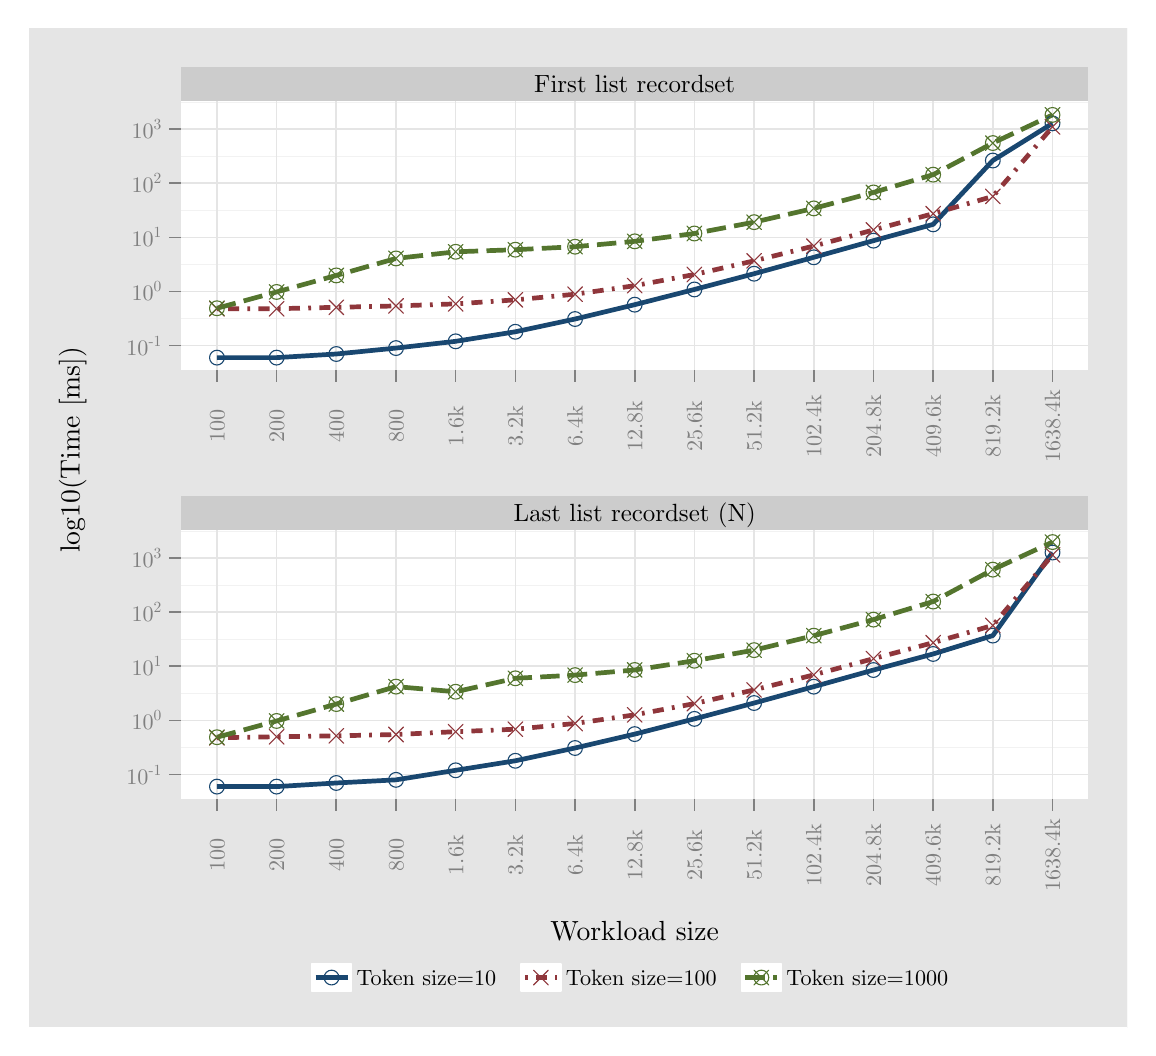
\begin{tikzpicture}[x=1pt,y=1pt]
\definecolor[named]{fillColor}{rgb}{1.00,1.00,1.00}
\path[use as bounding box,fill=fillColor,fill opacity=0.00] (0,0) rectangle (397.48,361.35);
\begin{scope}
\path[clip] (  0.00,  0.00) rectangle (397.48,361.35);
\definecolor[named]{drawColor}{rgb}{1.00,1.00,1.00}
\definecolor[named]{fillColor}{rgb}{0.90,0.90,0.90}

\path[draw=drawColor,line width= 0.6pt,line join=round,line cap=round,fill=fillColor] (  0.00, -0.00) rectangle (397.48,361.35);
\end{scope}
\begin{scope}
\path[clip] ( 55.45,237.71) rectangle (383.26,334.90);
\definecolor[named]{fillColor}{rgb}{1.00,1.00,1.00}

\path[fill=fillColor] ( 55.45,237.71) rectangle (383.26,334.90);
\definecolor[named]{drawColor}{rgb}{0.95,0.95,0.95}

\path[draw=drawColor,line width= 0.3pt,line join=round] ( 55.45,256.24) --
	(383.26,256.24);

\path[draw=drawColor,line width= 0.3pt,line join=round] ( 55.45,275.80) --
	(383.26,275.80);

\path[draw=drawColor,line width= 0.3pt,line join=round] ( 55.45,295.36) --
	(383.26,295.36);

\path[draw=drawColor,line width= 0.3pt,line join=round] ( 55.45,314.92) --
	(383.26,314.92);

\path[draw=drawColor,line width= 0.3pt,line join=round] ( 55.45,334.48) --
	(383.26,334.48);
\definecolor[named]{drawColor}{rgb}{0.90,0.90,0.90}

\path[draw=drawColor,line width= 0.6pt,line join=round] ( 55.45,246.46) --
	(383.26,246.46);

\path[draw=drawColor,line width= 0.6pt,line join=round] ( 55.45,266.02) --
	(383.26,266.02);

\path[draw=drawColor,line width= 0.6pt,line join=round] ( 55.45,285.58) --
	(383.26,285.58);

\path[draw=drawColor,line width= 0.6pt,line join=round] ( 55.45,305.14) --
	(383.26,305.14);

\path[draw=drawColor,line width= 0.6pt,line join=round] ( 55.45,324.70) --
	(383.26,324.70);

\path[draw=drawColor,line width= 0.6pt,line join=round] ( 68.39,237.71) --
	( 68.39,334.90);

\path[draw=drawColor,line width= 0.6pt,line join=round] ( 89.95,237.71) --
	( 89.95,334.90);

\path[draw=drawColor,line width= 0.6pt,line join=round] (111.52,237.71) --
	(111.52,334.90);

\path[draw=drawColor,line width= 0.6pt,line join=round] (133.09,237.71) --
	(133.09,334.90);

\path[draw=drawColor,line width= 0.6pt,line join=round] (154.65,237.71) --
	(154.65,334.90);

\path[draw=drawColor,line width= 0.6pt,line join=round] (176.22,237.71) --
	(176.22,334.90);

\path[draw=drawColor,line width= 0.6pt,line join=round] (197.79,237.71) --
	(197.79,334.90);

\path[draw=drawColor,line width= 0.6pt,line join=round] (219.35,237.71) --
	(219.35,334.90);

\path[draw=drawColor,line width= 0.6pt,line join=round] (240.92,237.71) --
	(240.92,334.90);

\path[draw=drawColor,line width= 0.6pt,line join=round] (262.49,237.71) --
	(262.49,334.90);

\path[draw=drawColor,line width= 0.6pt,line join=round] (284.05,237.71) --
	(284.05,334.90);

\path[draw=drawColor,line width= 0.6pt,line join=round] (305.62,237.71) --
	(305.62,334.90);

\path[draw=drawColor,line width= 0.6pt,line join=round] (327.19,237.71) --
	(327.19,334.90);

\path[draw=drawColor,line width= 0.6pt,line join=round] (348.75,237.71) --
	(348.75,334.90);

\path[draw=drawColor,line width= 0.6pt,line join=round] (370.32,237.71) --
	(370.32,334.90);
\definecolor[named]{drawColor}{rgb}{0.10,0.28,0.44}

\path[draw=drawColor,line width= 1.7pt,line join=round] ( 68.39,242.12) --
	( 89.95,242.12) --
	(111.52,243.43) --
	(133.09,245.57) --
	(154.65,248.01) --
	(176.22,251.46) --
	(197.79,256.07) --
	(219.35,261.25) --
	(240.92,266.75) --
	(262.49,272.44) --
	(284.05,278.37) --
	(305.62,284.38) --
	(327.19,290.27) --
	(348.75,313.34) --
	(370.32,326.77);
\definecolor[named]{drawColor}{rgb}{0.56,0.21,0.23}

\path[draw=drawColor,line width= 1.7pt,dash pattern=on 1pt off 3pt on 4pt off 3pt ,line join=round] ( 68.39,259.79) --
	( 89.95,259.79) --
	(111.52,260.30) --
	(133.09,260.79) --
	(154.65,261.54) --
	(176.22,262.99) --
	(197.79,265.03) --
	(219.35,268.12) --
	(240.92,272.16) --
	(262.49,277.09) --
	(284.05,282.44) --
	(305.62,288.25) --
	(327.19,294.14) --
	(348.75,300.37) --
	(370.32,325.48);
\definecolor[named]{drawColor}{rgb}{0.33,0.46,0.18}

\path[draw=drawColor,line width= 1.7pt,dash pattern=on 7pt off 3pt ,line join=round] ( 68.39,259.96) --
	( 89.95,265.85) --
	(111.52,271.82) --
	(133.09,277.96) --
	(154.65,280.36) --
	(176.22,281.11) --
	(197.79,282.20) --
	(219.35,284.14) --
	(240.92,286.97) --
	(262.49,291.07) --
	(284.05,296.04) --
	(305.62,301.81) --
	(327.19,308.23) --
	(348.75,319.65) --
	(370.32,329.82);
\definecolor[named]{drawColor}{rgb}{0.10,0.28,0.44}

\path[draw=drawColor,line width= 0.4pt,line join=round,line cap=round] ( 68.39,242.12) circle (  2.67);

\path[draw=drawColor,line width= 0.4pt,line join=round,line cap=round] ( 89.95,242.12) circle (  2.67);

\path[draw=drawColor,line width= 0.4pt,line join=round,line cap=round] (111.52,243.43) circle (  2.67);

\path[draw=drawColor,line width= 0.4pt,line join=round,line cap=round] (133.09,245.57) circle (  2.67);

\path[draw=drawColor,line width= 0.4pt,line join=round,line cap=round] (154.65,248.01) circle (  2.67);

\path[draw=drawColor,line width= 0.4pt,line join=round,line cap=round] (176.22,251.46) circle (  2.67);

\path[draw=drawColor,line width= 0.4pt,line join=round,line cap=round] (197.79,256.07) circle (  2.67);

\path[draw=drawColor,line width= 0.4pt,line join=round,line cap=round] (219.35,261.25) circle (  2.67);

\path[draw=drawColor,line width= 0.4pt,line join=round,line cap=round] (240.92,266.75) circle (  2.67);

\path[draw=drawColor,line width= 0.4pt,line join=round,line cap=round] (262.49,272.44) circle (  2.67);

\path[draw=drawColor,line width= 0.4pt,line join=round,line cap=round] (284.05,278.37) circle (  2.67);

\path[draw=drawColor,line width= 0.4pt,line join=round,line cap=round] (305.62,284.38) circle (  2.67);

\path[draw=drawColor,line width= 0.4pt,line join=round,line cap=round] (327.19,290.27) circle (  2.67);

\path[draw=drawColor,line width= 0.4pt,line join=round,line cap=round] (348.75,313.34) circle (  2.67);

\path[draw=drawColor,line width= 0.4pt,line join=round,line cap=round] (370.32,326.77) circle (  2.67);
\definecolor[named]{drawColor}{rgb}{0.56,0.21,0.23}

\path[draw=drawColor,line width= 0.4pt,line join=round,line cap=round,fill=fillColor] ( 65.72,257.12) -- ( 71.06,262.45);

\path[draw=drawColor,line width= 0.4pt,line join=round,line cap=round,fill=fillColor] ( 65.72,262.45) -- ( 71.06,257.12);

\path[draw=drawColor,line width= 0.4pt,line join=round,line cap=round,fill=fillColor] ( 87.29,257.12) -- ( 92.62,262.45);

\path[draw=drawColor,line width= 0.4pt,line join=round,line cap=round,fill=fillColor] ( 87.29,262.45) -- ( 92.62,257.12);

\path[draw=drawColor,line width= 0.4pt,line join=round,line cap=round,fill=fillColor] (108.85,257.63) -- (114.19,262.97);

\path[draw=drawColor,line width= 0.4pt,line join=round,line cap=round,fill=fillColor] (108.85,262.97) -- (114.19,257.63);

\path[draw=drawColor,line width= 0.4pt,line join=round,line cap=round,fill=fillColor] (130.42,258.12) -- (135.76,263.45);

\path[draw=drawColor,line width= 0.4pt,line join=round,line cap=round,fill=fillColor] (130.42,263.45) -- (135.76,258.12);

\path[draw=drawColor,line width= 0.4pt,line join=round,line cap=round,fill=fillColor] (151.99,258.87) -- (157.32,264.21);

\path[draw=drawColor,line width= 0.4pt,line join=round,line cap=round,fill=fillColor] (151.99,264.21) -- (157.32,258.87);

\path[draw=drawColor,line width= 0.4pt,line join=round,line cap=round,fill=fillColor] (173.55,260.32) -- (178.89,265.66);

\path[draw=drawColor,line width= 0.4pt,line join=round,line cap=round,fill=fillColor] (173.55,265.66) -- (178.89,260.32);

\path[draw=drawColor,line width= 0.4pt,line join=round,line cap=round,fill=fillColor] (195.12,262.36) -- (200.45,267.70);

\path[draw=drawColor,line width= 0.4pt,line join=round,line cap=round,fill=fillColor] (195.12,267.70) -- (200.45,262.36);

\path[draw=drawColor,line width= 0.4pt,line join=round,line cap=round,fill=fillColor] (216.69,265.45) -- (222.02,270.79);

\path[draw=drawColor,line width= 0.4pt,line join=round,line cap=round,fill=fillColor] (216.69,270.79) -- (222.02,265.45);

\path[draw=drawColor,line width= 0.4pt,line join=round,line cap=round,fill=fillColor] (238.25,269.49) -- (243.59,274.83);

\path[draw=drawColor,line width= 0.4pt,line join=round,line cap=round,fill=fillColor] (238.25,274.83) -- (243.59,269.49);

\path[draw=drawColor,line width= 0.4pt,line join=round,line cap=round,fill=fillColor] (259.82,274.42) -- (265.15,279.76);

\path[draw=drawColor,line width= 0.4pt,line join=round,line cap=round,fill=fillColor] (259.82,279.76) -- (265.15,274.42);

\path[draw=drawColor,line width= 0.4pt,line join=round,line cap=round,fill=fillColor] (281.39,279.77) -- (286.72,285.11);

\path[draw=drawColor,line width= 0.4pt,line join=round,line cap=round,fill=fillColor] (281.39,285.11) -- (286.72,279.77);

\path[draw=drawColor,line width= 0.4pt,line join=round,line cap=round,fill=fillColor] (302.95,285.59) -- (308.29,290.92);

\path[draw=drawColor,line width= 0.4pt,line join=round,line cap=round,fill=fillColor] (302.95,290.92) -- (308.29,285.59);

\path[draw=drawColor,line width= 0.4pt,line join=round,line cap=round,fill=fillColor] (324.52,291.47) -- (329.85,296.81);

\path[draw=drawColor,line width= 0.4pt,line join=round,line cap=round,fill=fillColor] (324.52,296.81) -- (329.85,291.47);

\path[draw=drawColor,line width= 0.4pt,line join=round,line cap=round,fill=fillColor] (346.08,297.70) -- (351.42,303.03);

\path[draw=drawColor,line width= 0.4pt,line join=round,line cap=round,fill=fillColor] (346.08,303.03) -- (351.42,297.70);

\path[draw=drawColor,line width= 0.4pt,line join=round,line cap=round,fill=fillColor] (367.65,322.81) -- (372.99,328.15);

\path[draw=drawColor,line width= 0.4pt,line join=round,line cap=round,fill=fillColor] (367.65,328.15) -- (372.99,322.81);
\definecolor[named]{drawColor}{rgb}{0.33,0.46,0.18}

\path[draw=drawColor,line width= 0.4pt,line join=round,line cap=round] ( 68.39,259.96) circle (  2.67);

\path[draw=drawColor,line width= 0.4pt,line join=round,line cap=round] ( 65.72,257.29) -- ( 71.06,262.63);

\path[draw=drawColor,line width= 0.4pt,line join=round,line cap=round] ( 65.72,262.63) -- ( 71.06,257.29);

\path[draw=drawColor,line width= 0.4pt,line join=round,line cap=round] ( 89.95,265.85) circle (  2.67);

\path[draw=drawColor,line width= 0.4pt,line join=round,line cap=round] ( 87.29,263.18) -- ( 92.62,268.52);

\path[draw=drawColor,line width= 0.4pt,line join=round,line cap=round] ( 87.29,268.52) -- ( 92.62,263.18);

\path[draw=drawColor,line width= 0.4pt,line join=round,line cap=round] (111.52,271.82) circle (  2.67);

\path[draw=drawColor,line width= 0.4pt,line join=round,line cap=round] (108.85,269.16) -- (114.19,274.49);

\path[draw=drawColor,line width= 0.4pt,line join=round,line cap=round] (108.85,274.49) -- (114.19,269.16);

\path[draw=drawColor,line width= 0.4pt,line join=round,line cap=round] (133.09,277.96) circle (  2.67);

\path[draw=drawColor,line width= 0.4pt,line join=round,line cap=round] (130.42,275.30) -- (135.76,280.63);

\path[draw=drawColor,line width= 0.4pt,line join=round,line cap=round] (130.42,280.63) -- (135.76,275.30);

\path[draw=drawColor,line width= 0.4pt,line join=round,line cap=round] (154.65,280.36) circle (  2.67);

\path[draw=drawColor,line width= 0.4pt,line join=round,line cap=round] (151.99,277.69) -- (157.32,283.03);

\path[draw=drawColor,line width= 0.4pt,line join=round,line cap=round] (151.99,283.03) -- (157.32,277.69);

\path[draw=drawColor,line width= 0.4pt,line join=round,line cap=round] (176.22,281.11) circle (  2.67);

\path[draw=drawColor,line width= 0.4pt,line join=round,line cap=round] (173.55,278.44) -- (178.89,283.78);

\path[draw=drawColor,line width= 0.4pt,line join=round,line cap=round] (173.55,283.78) -- (178.89,278.44);

\path[draw=drawColor,line width= 0.4pt,line join=round,line cap=round] (197.79,282.20) circle (  2.67);

\path[draw=drawColor,line width= 0.4pt,line join=round,line cap=round] (195.12,279.54) -- (200.45,284.87);

\path[draw=drawColor,line width= 0.4pt,line join=round,line cap=round] (195.12,284.87) -- (200.45,279.54);

\path[draw=drawColor,line width= 0.4pt,line join=round,line cap=round] (219.35,284.14) circle (  2.67);

\path[draw=drawColor,line width= 0.4pt,line join=round,line cap=round] (216.69,281.47) -- (222.02,286.81);

\path[draw=drawColor,line width= 0.4pt,line join=round,line cap=round] (216.69,286.81) -- (222.02,281.47);

\path[draw=drawColor,line width= 0.4pt,line join=round,line cap=round] (240.92,286.97) circle (  2.67);

\path[draw=drawColor,line width= 0.4pt,line join=round,line cap=round] (238.25,284.30) -- (243.59,289.64);

\path[draw=drawColor,line width= 0.4pt,line join=round,line cap=round] (238.25,289.64) -- (243.59,284.30);

\path[draw=drawColor,line width= 0.4pt,line join=round,line cap=round] (262.49,291.07) circle (  2.67);

\path[draw=drawColor,line width= 0.4pt,line join=round,line cap=round] (259.82,288.40) -- (265.15,293.74);

\path[draw=drawColor,line width= 0.4pt,line join=round,line cap=round] (259.82,293.74) -- (265.15,288.40);

\path[draw=drawColor,line width= 0.4pt,line join=round,line cap=round] (284.05,296.04) circle (  2.67);

\path[draw=drawColor,line width= 0.4pt,line join=round,line cap=round] (281.39,293.37) -- (286.72,298.71);

\path[draw=drawColor,line width= 0.4pt,line join=round,line cap=round] (281.39,298.71) -- (286.72,293.37);

\path[draw=drawColor,line width= 0.4pt,line join=round,line cap=round] (305.62,301.81) circle (  2.67);

\path[draw=drawColor,line width= 0.4pt,line join=round,line cap=round] (302.95,299.14) -- (308.29,304.48);

\path[draw=drawColor,line width= 0.4pt,line join=round,line cap=round] (302.95,304.48) -- (308.29,299.14);

\path[draw=drawColor,line width= 0.4pt,line join=round,line cap=round] (327.19,308.23) circle (  2.67);

\path[draw=drawColor,line width= 0.4pt,line join=round,line cap=round] (324.52,305.56) -- (329.85,310.89);

\path[draw=drawColor,line width= 0.4pt,line join=round,line cap=round] (324.52,310.89) -- (329.85,305.56);

\path[draw=drawColor,line width= 0.4pt,line join=round,line cap=round] (348.75,319.65) circle (  2.67);

\path[draw=drawColor,line width= 0.4pt,line join=round,line cap=round] (346.08,316.99) -- (351.42,322.32);

\path[draw=drawColor,line width= 0.4pt,line join=round,line cap=round] (346.08,322.32) -- (351.42,316.99);

\path[draw=drawColor,line width= 0.4pt,line join=round,line cap=round] (370.32,329.82) circle (  2.67);

\path[draw=drawColor,line width= 0.4pt,line join=round,line cap=round] (367.65,327.15) -- (372.99,332.49);

\path[draw=drawColor,line width= 0.4pt,line join=round,line cap=round] (367.65,332.49) -- (372.99,327.15);
\end{scope}
\begin{scope}
\path[clip] ( 55.45, 82.69) rectangle (383.26,179.89);
\definecolor[named]{fillColor}{rgb}{1.00,1.00,1.00}

\path[fill=fillColor] ( 55.45, 82.69) rectangle (383.26,179.89);
\definecolor[named]{drawColor}{rgb}{0.95,0.95,0.95}

\path[draw=drawColor,line width= 0.3pt,line join=round] ( 55.45,101.23) --
	(383.26,101.23);

\path[draw=drawColor,line width= 0.3pt,line join=round] ( 55.45,120.79) --
	(383.26,120.79);

\path[draw=drawColor,line width= 0.3pt,line join=round] ( 55.45,140.34) --
	(383.26,140.34);

\path[draw=drawColor,line width= 0.3pt,line join=round] ( 55.45,159.90) --
	(383.26,159.90);

\path[draw=drawColor,line width= 0.3pt,line join=round] ( 55.45,179.46) --
	(383.26,179.46);
\definecolor[named]{drawColor}{rgb}{0.90,0.90,0.90}

\path[draw=drawColor,line width= 0.6pt,line join=round] ( 55.45, 91.45) --
	(383.26, 91.45);

\path[draw=drawColor,line width= 0.6pt,line join=round] ( 55.45,111.01) --
	(383.26,111.01);

\path[draw=drawColor,line width= 0.6pt,line join=round] ( 55.45,130.57) --
	(383.26,130.57);

\path[draw=drawColor,line width= 0.6pt,line join=round] ( 55.45,150.12) --
	(383.26,150.12);

\path[draw=drawColor,line width= 0.6pt,line join=round] ( 55.45,169.68) --
	(383.26,169.68);

\path[draw=drawColor,line width= 0.6pt,line join=round] ( 68.39, 82.69) --
	( 68.39,179.89);

\path[draw=drawColor,line width= 0.6pt,line join=round] ( 89.95, 82.69) --
	( 89.95,179.89);

\path[draw=drawColor,line width= 0.6pt,line join=round] (111.52, 82.69) --
	(111.52,179.89);

\path[draw=drawColor,line width= 0.6pt,line join=round] (133.09, 82.69) --
	(133.09,179.89);

\path[draw=drawColor,line width= 0.6pt,line join=round] (154.65, 82.69) --
	(154.65,179.89);

\path[draw=drawColor,line width= 0.6pt,line join=round] (176.22, 82.69) --
	(176.22,179.89);

\path[draw=drawColor,line width= 0.6pt,line join=round] (197.79, 82.69) --
	(197.79,179.89);

\path[draw=drawColor,line width= 0.6pt,line join=round] (219.35, 82.69) --
	(219.35,179.89);

\path[draw=drawColor,line width= 0.6pt,line join=round] (240.92, 82.69) --
	(240.92,179.89);

\path[draw=drawColor,line width= 0.6pt,line join=round] (262.49, 82.69) --
	(262.49,179.89);

\path[draw=drawColor,line width= 0.6pt,line join=round] (284.05, 82.69) --
	(284.05,179.89);

\path[draw=drawColor,line width= 0.6pt,line join=round] (305.62, 82.69) --
	(305.62,179.89);

\path[draw=drawColor,line width= 0.6pt,line join=round] (327.19, 82.69) --
	(327.19,179.89);

\path[draw=drawColor,line width= 0.6pt,line join=round] (348.75, 82.69) --
	(348.75,179.89);

\path[draw=drawColor,line width= 0.6pt,line join=round] (370.32, 82.69) --
	(370.32,179.89);
\definecolor[named]{drawColor}{rgb}{0.10,0.28,0.44}

\path[draw=drawColor,line width= 1.7pt,line join=round] ( 68.39, 87.11) --
	( 89.95, 87.11) --
	(111.52, 88.42) --
	(133.09, 89.55) --
	(154.65, 93.00) --
	(176.22, 96.44) --
	(197.79,101.06) --
	(219.35,106.08) --
	(240.92,111.58) --
	(262.49,117.31) --
	(284.05,123.22) --
	(305.62,129.23) --
	(327.19,135.04) --
	(348.75,141.68) --
	(370.32,171.69);
\definecolor[named]{drawColor}{rgb}{0.56,0.21,0.23}

\path[draw=drawColor,line width= 1.7pt,dash pattern=on 1pt off 3pt on 4pt off 3pt ,line join=round] ( 68.39,104.77) --
	( 89.95,105.12) --
	(111.52,105.45) --
	(133.09,105.93) --
	(154.65,106.95) --
	(176.22,107.85) --
	(197.79,109.92) --
	(219.35,113.04) --
	(240.92,117.10) --
	(262.49,122.05) --
	(284.05,127.49) --
	(305.62,133.34) --
	(327.19,139.12) --
	(348.75,145.35) --
	(370.32,170.84);
\definecolor[named]{drawColor}{rgb}{0.33,0.46,0.18}

\path[draw=drawColor,line width= 1.7pt,dash pattern=on 7pt off 3pt ,line join=round] ( 68.39,104.95) --
	( 89.95,110.83) --
	(111.52,116.94) --
	(133.09,123.24) --
	(154.65,121.38) --
	(176.22,126.24) --
	(197.79,127.40) --
	(219.35,129.25) --
	(240.92,132.59) --
	(262.49,136.42) --
	(284.05,141.64) --
	(305.62,147.45) --
	(327.19,153.98) --
	(348.75,165.51) --
	(370.32,175.47);
\definecolor[named]{drawColor}{rgb}{0.10,0.28,0.44}

\path[draw=drawColor,line width= 0.4pt,line join=round,line cap=round] ( 68.39, 87.11) circle (  2.67);

\path[draw=drawColor,line width= 0.4pt,line join=round,line cap=round] ( 89.95, 87.11) circle (  2.67);

\path[draw=drawColor,line width= 0.4pt,line join=round,line cap=round] (111.52, 88.42) circle (  2.67);

\path[draw=drawColor,line width= 0.4pt,line join=round,line cap=round] (133.09, 89.55) circle (  2.67);

\path[draw=drawColor,line width= 0.4pt,line join=round,line cap=round] (154.65, 93.00) circle (  2.67);

\path[draw=drawColor,line width= 0.4pt,line join=round,line cap=round] (176.22, 96.44) circle (  2.67);

\path[draw=drawColor,line width= 0.4pt,line join=round,line cap=round] (197.79,101.06) circle (  2.67);

\path[draw=drawColor,line width= 0.4pt,line join=round,line cap=round] (219.35,106.08) circle (  2.67);

\path[draw=drawColor,line width= 0.4pt,line join=round,line cap=round] (240.92,111.58) circle (  2.67);

\path[draw=drawColor,line width= 0.4pt,line join=round,line cap=round] (262.49,117.31) circle (  2.67);

\path[draw=drawColor,line width= 0.4pt,line join=round,line cap=round] (284.05,123.22) circle (  2.67);

\path[draw=drawColor,line width= 0.4pt,line join=round,line cap=round] (305.62,129.23) circle (  2.67);

\path[draw=drawColor,line width= 0.4pt,line join=round,line cap=round] (327.19,135.04) circle (  2.67);

\path[draw=drawColor,line width= 0.4pt,line join=round,line cap=round] (348.75,141.68) circle (  2.67);

\path[draw=drawColor,line width= 0.4pt,line join=round,line cap=round] (370.32,171.69) circle (  2.67);
\definecolor[named]{drawColor}{rgb}{0.56,0.21,0.23}

\path[draw=drawColor,line width= 0.4pt,line join=round,line cap=round,fill=fillColor] ( 65.72,102.10) -- ( 71.06,107.44);

\path[draw=drawColor,line width= 0.4pt,line join=round,line cap=round,fill=fillColor] ( 65.72,107.44) -- ( 71.06,102.10);

\path[draw=drawColor,line width= 0.4pt,line join=round,line cap=round,fill=fillColor] ( 87.29,102.45) -- ( 92.62,107.79);

\path[draw=drawColor,line width= 0.4pt,line join=round,line cap=round,fill=fillColor] ( 87.29,107.79) -- ( 92.62,102.45);

\path[draw=drawColor,line width= 0.4pt,line join=round,line cap=round,fill=fillColor] (108.85,102.78) -- (114.19,108.12);

\path[draw=drawColor,line width= 0.4pt,line join=round,line cap=round,fill=fillColor] (108.85,108.12) -- (114.19,102.78);

\path[draw=drawColor,line width= 0.4pt,line join=round,line cap=round,fill=fillColor] (130.42,103.26) -- (135.76,108.60);

\path[draw=drawColor,line width= 0.4pt,line join=round,line cap=round,fill=fillColor] (130.42,108.60) -- (135.76,103.26);

\path[draw=drawColor,line width= 0.4pt,line join=round,line cap=round,fill=fillColor] (151.99,104.28) -- (157.32,109.61);

\path[draw=drawColor,line width= 0.4pt,line join=round,line cap=round,fill=fillColor] (151.99,109.61) -- (157.32,104.28);

\path[draw=drawColor,line width= 0.4pt,line join=round,line cap=round,fill=fillColor] (173.55,105.19) -- (178.89,110.52);

\path[draw=drawColor,line width= 0.4pt,line join=round,line cap=round,fill=fillColor] (173.55,110.52) -- (178.89,105.19);

\path[draw=drawColor,line width= 0.4pt,line join=round,line cap=round,fill=fillColor] (195.12,107.25) -- (200.45,112.59);

\path[draw=drawColor,line width= 0.4pt,line join=round,line cap=round,fill=fillColor] (195.12,112.59) -- (200.45,107.25);

\path[draw=drawColor,line width= 0.4pt,line join=round,line cap=round,fill=fillColor] (216.69,110.37) -- (222.02,115.70);

\path[draw=drawColor,line width= 0.4pt,line join=round,line cap=round,fill=fillColor] (216.69,115.70) -- (222.02,110.37);

\path[draw=drawColor,line width= 0.4pt,line join=round,line cap=round,fill=fillColor] (238.25,114.44) -- (243.59,119.77);

\path[draw=drawColor,line width= 0.4pt,line join=round,line cap=round,fill=fillColor] (238.25,119.77) -- (243.59,114.44);

\path[draw=drawColor,line width= 0.4pt,line join=round,line cap=round,fill=fillColor] (259.82,119.38) -- (265.15,124.72);

\path[draw=drawColor,line width= 0.4pt,line join=round,line cap=round,fill=fillColor] (259.82,124.72) -- (265.15,119.38);

\path[draw=drawColor,line width= 0.4pt,line join=round,line cap=round,fill=fillColor] (281.39,124.82) -- (286.72,130.15);

\path[draw=drawColor,line width= 0.4pt,line join=round,line cap=round,fill=fillColor] (281.39,130.15) -- (286.72,124.82);

\path[draw=drawColor,line width= 0.4pt,line join=round,line cap=round,fill=fillColor] (302.95,130.67) -- (308.29,136.01);

\path[draw=drawColor,line width= 0.4pt,line join=round,line cap=round,fill=fillColor] (302.95,136.01) -- (308.29,130.67);

\path[draw=drawColor,line width= 0.4pt,line join=round,line cap=round,fill=fillColor] (324.52,136.45) -- (329.85,141.79);

\path[draw=drawColor,line width= 0.4pt,line join=round,line cap=round,fill=fillColor] (324.52,141.79) -- (329.85,136.45);

\path[draw=drawColor,line width= 0.4pt,line join=round,line cap=round,fill=fillColor] (346.08,142.68) -- (351.42,148.02);

\path[draw=drawColor,line width= 0.4pt,line join=round,line cap=round,fill=fillColor] (346.08,148.02) -- (351.42,142.68);

\path[draw=drawColor,line width= 0.4pt,line join=round,line cap=round,fill=fillColor] (367.65,168.17) -- (372.99,173.50);

\path[draw=drawColor,line width= 0.4pt,line join=round,line cap=round,fill=fillColor] (367.65,173.50) -- (372.99,168.17);
\definecolor[named]{drawColor}{rgb}{0.33,0.46,0.18}

\path[draw=drawColor,line width= 0.4pt,line join=round,line cap=round] ( 68.39,104.95) circle (  2.67);

\path[draw=drawColor,line width= 0.4pt,line join=round,line cap=round] ( 65.72,102.28) -- ( 71.06,107.61);

\path[draw=drawColor,line width= 0.4pt,line join=round,line cap=round] ( 65.72,107.61) -- ( 71.06,102.28);

\path[draw=drawColor,line width= 0.4pt,line join=round,line cap=round] ( 89.95,110.83) circle (  2.67);

\path[draw=drawColor,line width= 0.4pt,line join=round,line cap=round] ( 87.29,108.17) -- ( 92.62,113.50);

\path[draw=drawColor,line width= 0.4pt,line join=round,line cap=round] ( 87.29,113.50) -- ( 92.62,108.17);

\path[draw=drawColor,line width= 0.4pt,line join=round,line cap=round] (111.52,116.94) circle (  2.67);

\path[draw=drawColor,line width= 0.4pt,line join=round,line cap=round] (108.85,114.27) -- (114.19,119.60);

\path[draw=drawColor,line width= 0.4pt,line join=round,line cap=round] (108.85,119.60) -- (114.19,114.27);

\path[draw=drawColor,line width= 0.4pt,line join=round,line cap=round] (133.09,123.24) circle (  2.67);

\path[draw=drawColor,line width= 0.4pt,line join=round,line cap=round] (130.42,120.57) -- (135.76,125.90);

\path[draw=drawColor,line width= 0.4pt,line join=round,line cap=round] (130.42,125.90) -- (135.76,120.57);

\path[draw=drawColor,line width= 0.4pt,line join=round,line cap=round] (154.65,121.38) circle (  2.67);

\path[draw=drawColor,line width= 0.4pt,line join=round,line cap=round] (151.99,118.71) -- (157.32,124.04);

\path[draw=drawColor,line width= 0.4pt,line join=round,line cap=round] (151.99,124.04) -- (157.32,118.71);

\path[draw=drawColor,line width= 0.4pt,line join=round,line cap=round] (176.22,126.24) circle (  2.67);

\path[draw=drawColor,line width= 0.4pt,line join=round,line cap=round] (173.55,123.57) -- (178.89,128.91);

\path[draw=drawColor,line width= 0.4pt,line join=round,line cap=round] (173.55,128.91) -- (178.89,123.57);

\path[draw=drawColor,line width= 0.4pt,line join=round,line cap=round] (197.79,127.40) circle (  2.67);

\path[draw=drawColor,line width= 0.4pt,line join=round,line cap=round] (195.12,124.73) -- (200.45,130.07);

\path[draw=drawColor,line width= 0.4pt,line join=round,line cap=round] (195.12,130.07) -- (200.45,124.73);

\path[draw=drawColor,line width= 0.4pt,line join=round,line cap=round] (219.35,129.25) circle (  2.67);

\path[draw=drawColor,line width= 0.4pt,line join=round,line cap=round] (216.69,126.59) -- (222.02,131.92);

\path[draw=drawColor,line width= 0.4pt,line join=round,line cap=round] (216.69,131.92) -- (222.02,126.59);

\path[draw=drawColor,line width= 0.4pt,line join=round,line cap=round] (240.92,132.59) circle (  2.67);

\path[draw=drawColor,line width= 0.4pt,line join=round,line cap=round] (238.25,129.92) -- (243.59,135.26);

\path[draw=drawColor,line width= 0.4pt,line join=round,line cap=round] (238.25,135.26) -- (243.59,129.92);

\path[draw=drawColor,line width= 0.4pt,line join=round,line cap=round] (262.49,136.42) circle (  2.67);

\path[draw=drawColor,line width= 0.4pt,line join=round,line cap=round] (259.82,133.75) -- (265.15,139.09);

\path[draw=drawColor,line width= 0.4pt,line join=round,line cap=round] (259.82,139.09) -- (265.15,133.75);

\path[draw=drawColor,line width= 0.4pt,line join=round,line cap=round] (284.05,141.64) circle (  2.67);

\path[draw=drawColor,line width= 0.4pt,line join=round,line cap=round] (281.39,138.98) -- (286.72,144.31);

\path[draw=drawColor,line width= 0.4pt,line join=round,line cap=round] (281.39,144.31) -- (286.72,138.98);

\path[draw=drawColor,line width= 0.4pt,line join=round,line cap=round] (305.62,147.45) circle (  2.67);

\path[draw=drawColor,line width= 0.4pt,line join=round,line cap=round] (302.95,144.79) -- (308.29,150.12);

\path[draw=drawColor,line width= 0.4pt,line join=round,line cap=round] (302.95,150.12) -- (308.29,144.79);

\path[draw=drawColor,line width= 0.4pt,line join=round,line cap=round] (327.19,153.98) circle (  2.67);

\path[draw=drawColor,line width= 0.4pt,line join=round,line cap=round] (324.52,151.31) -- (329.85,156.65);

\path[draw=drawColor,line width= 0.4pt,line join=round,line cap=round] (324.52,156.65) -- (329.85,151.31);

\path[draw=drawColor,line width= 0.4pt,line join=round,line cap=round] (348.75,165.51) circle (  2.67);

\path[draw=drawColor,line width= 0.4pt,line join=round,line cap=round] (346.08,162.84) -- (351.42,168.18);

\path[draw=drawColor,line width= 0.4pt,line join=round,line cap=round] (346.08,168.18) -- (351.42,162.84);

\path[draw=drawColor,line width= 0.4pt,line join=round,line cap=round] (370.32,175.47) circle (  2.67);

\path[draw=drawColor,line width= 0.4pt,line join=round,line cap=round] (367.65,172.80) -- (372.99,178.14);

\path[draw=drawColor,line width= 0.4pt,line join=round,line cap=round] (367.65,178.14) -- (372.99,172.80);
\end{scope}
\begin{scope}
\path[clip] (  0.00,  0.00) rectangle (397.48,361.35);
\definecolor[named]{fillColor}{rgb}{0.80,0.80,0.80}

\path[fill=fillColor] ( 55.45,334.90) rectangle (383.26,347.12);
\definecolor[named]{drawColor}{rgb}{0.00,0.00,0.00}

\node[text=drawColor,anchor=base,inner sep=0pt, outer sep=0pt, scale=  0.90] at (219.35,337.91) {First list recordset };
\end{scope}
\begin{scope}
\path[clip] (  0.00,  0.00) rectangle (397.48,361.35);
\definecolor[named]{fillColor}{rgb}{0.80,0.80,0.80}

\path[fill=fillColor] ( 55.45,179.89) rectangle (383.26,192.11);
\definecolor[named]{drawColor}{rgb}{0.00,0.00,0.00}

\node[text=drawColor,anchor=base,inner sep=0pt, outer sep=0pt, scale=  0.90] at (219.35,182.90) {Last list recordset (N) };
\end{scope}
\begin{scope}
\path[clip] (  0.00,  0.00) rectangle (397.48,361.35);
\definecolor[named]{drawColor}{rgb}{0.50,0.50,0.50}

\node[text=drawColor,anchor=base west,inner sep=0pt, outer sep=0pt, scale=  0.80] at ( 35.67,243.03) {10};

\node[text=drawColor,anchor=base west,inner sep=0pt, outer sep=0pt, scale=  0.56] at ( 43.67,246.30) {-};

\node[text=drawColor,anchor=base west,inner sep=0pt, outer sep=0pt, scale=  0.56] at ( 45.54,246.30) {1};

\node[text=drawColor,anchor=base west,inner sep=0pt, outer sep=0pt, scale=  0.80] at ( 37.54,262.59) {10};

\node[text=drawColor,anchor=base west,inner sep=0pt, outer sep=0pt, scale=  0.56] at ( 45.54,265.86) {0};

\node[text=drawColor,anchor=base west,inner sep=0pt, outer sep=0pt, scale=  0.80] at ( 37.54,282.15) {10};

\node[text=drawColor,anchor=base west,inner sep=0pt, outer sep=0pt, scale=  0.56] at ( 45.54,285.42) {1};

\node[text=drawColor,anchor=base west,inner sep=0pt, outer sep=0pt, scale=  0.80] at ( 37.54,301.71) {10};

\node[text=drawColor,anchor=base west,inner sep=0pt, outer sep=0pt, scale=  0.56] at ( 45.54,304.98) {2};

\node[text=drawColor,anchor=base west,inner sep=0pt, outer sep=0pt, scale=  0.80] at ( 37.54,321.27) {10};

\node[text=drawColor,anchor=base west,inner sep=0pt, outer sep=0pt, scale=  0.56] at ( 45.54,324.54) {3};
\end{scope}
\begin{scope}
\path[clip] (  0.00,  0.00) rectangle (397.48,361.35);
\definecolor[named]{drawColor}{rgb}{0.50,0.50,0.50}

\path[draw=drawColor,line width= 0.6pt,line join=round] ( 51.18,246.46) --
	( 55.45,246.46);

\path[draw=drawColor,line width= 0.6pt,line join=round] ( 51.18,266.02) --
	( 55.45,266.02);

\path[draw=drawColor,line width= 0.6pt,line join=round] ( 51.18,285.58) --
	( 55.45,285.58);

\path[draw=drawColor,line width= 0.6pt,line join=round] ( 51.18,305.14) --
	( 55.45,305.14);

\path[draw=drawColor,line width= 0.6pt,line join=round] ( 51.18,324.70) --
	( 55.45,324.70);
\end{scope}
\begin{scope}
\path[clip] (  0.00,  0.00) rectangle (397.48,361.35);
\definecolor[named]{drawColor}{rgb}{0.50,0.50,0.50}

\node[text=drawColor,anchor=base west,inner sep=0pt, outer sep=0pt, scale=  0.80] at ( 35.67, 88.02) {10};

\node[text=drawColor,anchor=base west,inner sep=0pt, outer sep=0pt, scale=  0.56] at ( 43.67, 91.29) {-};

\node[text=drawColor,anchor=base west,inner sep=0pt, outer sep=0pt, scale=  0.56] at ( 45.54, 91.29) {1};

\node[text=drawColor,anchor=base west,inner sep=0pt, outer sep=0pt, scale=  0.80] at ( 37.54,107.57) {10};

\node[text=drawColor,anchor=base west,inner sep=0pt, outer sep=0pt, scale=  0.56] at ( 45.54,110.85) {0};

\node[text=drawColor,anchor=base west,inner sep=0pt, outer sep=0pt, scale=  0.80] at ( 37.54,127.13) {10};

\node[text=drawColor,anchor=base west,inner sep=0pt, outer sep=0pt, scale=  0.56] at ( 45.54,130.40) {1};

\node[text=drawColor,anchor=base west,inner sep=0pt, outer sep=0pt, scale=  0.80] at ( 37.54,146.69) {10};

\node[text=drawColor,anchor=base west,inner sep=0pt, outer sep=0pt, scale=  0.56] at ( 45.54,149.96) {2};

\node[text=drawColor,anchor=base west,inner sep=0pt, outer sep=0pt, scale=  0.80] at ( 37.54,166.25) {10};

\node[text=drawColor,anchor=base west,inner sep=0pt, outer sep=0pt, scale=  0.56] at ( 45.54,169.52) {3};
\end{scope}
\begin{scope}
\path[clip] (  0.00,  0.00) rectangle (397.48,361.35);
\definecolor[named]{drawColor}{rgb}{0.50,0.50,0.50}

\path[draw=drawColor,line width= 0.6pt,line join=round] ( 51.18, 91.45) --
	( 55.45, 91.45);

\path[draw=drawColor,line width= 0.6pt,line join=round] ( 51.18,111.01) --
	( 55.45,111.01);

\path[draw=drawColor,line width= 0.6pt,line join=round] ( 51.18,130.57) --
	( 55.45,130.57);

\path[draw=drawColor,line width= 0.6pt,line join=round] ( 51.18,150.12) --
	( 55.45,150.12);

\path[draw=drawColor,line width= 0.6pt,line join=round] ( 51.18,169.68) --
	( 55.45,169.68);
\end{scope}
\begin{scope}
\path[clip] (  0.00,  0.00) rectangle (397.48,361.35);
\definecolor[named]{drawColor}{rgb}{0.50,0.50,0.50}

\path[draw=drawColor,line width= 0.6pt,line join=round] ( 68.39,233.44) --
	( 68.39,237.71);

\path[draw=drawColor,line width= 0.6pt,line join=round] ( 89.95,233.44) --
	( 89.95,237.71);

\path[draw=drawColor,line width= 0.6pt,line join=round] (111.52,233.44) --
	(111.52,237.71);

\path[draw=drawColor,line width= 0.6pt,line join=round] (133.09,233.44) --
	(133.09,237.71);

\path[draw=drawColor,line width= 0.6pt,line join=round] (154.65,233.44) --
	(154.65,237.71);

\path[draw=drawColor,line width= 0.6pt,line join=round] (176.22,233.44) --
	(176.22,237.71);

\path[draw=drawColor,line width= 0.6pt,line join=round] (197.79,233.44) --
	(197.79,237.71);

\path[draw=drawColor,line width= 0.6pt,line join=round] (219.35,233.44) --
	(219.35,237.71);

\path[draw=drawColor,line width= 0.6pt,line join=round] (240.92,233.44) --
	(240.92,237.71);

\path[draw=drawColor,line width= 0.6pt,line join=round] (262.49,233.44) --
	(262.49,237.71);

\path[draw=drawColor,line width= 0.6pt,line join=round] (284.05,233.44) --
	(284.05,237.71);

\path[draw=drawColor,line width= 0.6pt,line join=round] (305.62,233.44) --
	(305.62,237.71);

\path[draw=drawColor,line width= 0.6pt,line join=round] (327.19,233.44) --
	(327.19,237.71);

\path[draw=drawColor,line width= 0.6pt,line join=round] (348.75,233.44) --
	(348.75,237.71);

\path[draw=drawColor,line width= 0.6pt,line join=round] (370.32,233.44) --
	(370.32,237.71);
\end{scope}
\begin{scope}
\path[clip] (  0.00,  0.00) rectangle (397.48,361.35);
\definecolor[named]{drawColor}{rgb}{0.50,0.50,0.50}

\node[text=drawColor,rotate= 90.00,anchor=base,inner sep=0pt, outer sep=0pt, scale=  0.80] at ( 71.14,217.37) {100};

\node[text=drawColor,rotate= 90.00,anchor=base,inner sep=0pt, outer sep=0pt, scale=  0.80] at ( 92.71,217.37) {200};

\node[text=drawColor,rotate= 90.00,anchor=base,inner sep=0pt, outer sep=0pt, scale=  0.80] at (114.28,217.37) {400};

\node[text=drawColor,rotate= 90.00,anchor=base,inner sep=0pt, outer sep=0pt, scale=  0.80] at (135.84,217.37) {800};

\node[text=drawColor,rotate= 90.00,anchor=base,inner sep=0pt, outer sep=0pt, scale=  0.80] at (157.41,217.37) {1.6k};

\node[text=drawColor,rotate= 90.00,anchor=base,inner sep=0pt, outer sep=0pt, scale=  0.80] at (178.98,217.37) {3.2k};

\node[text=drawColor,rotate= 90.00,anchor=base,inner sep=0pt, outer sep=0pt, scale=  0.80] at (200.54,217.37) {6.4k};

\node[text=drawColor,rotate= 90.00,anchor=base,inner sep=0pt, outer sep=0pt, scale=  0.80] at (222.11,217.37) {12.8k};

\node[text=drawColor,rotate= 90.00,anchor=base,inner sep=0pt, outer sep=0pt, scale=  0.80] at (243.67,217.37) {25.6k};

\node[text=drawColor,rotate= 90.00,anchor=base,inner sep=0pt, outer sep=0pt, scale=  0.80] at (265.24,217.37) {51.2k};

\node[text=drawColor,rotate= 90.00,anchor=base,inner sep=0pt, outer sep=0pt, scale=  0.80] at (286.81,217.37) {102.4k};

\node[text=drawColor,rotate= 90.00,anchor=base,inner sep=0pt, outer sep=0pt, scale=  0.80] at (308.37,217.37) {204.8k};

\node[text=drawColor,rotate= 90.00,anchor=base,inner sep=0pt, outer sep=0pt, scale=  0.80] at (329.94,217.37) {409.6k};

\node[text=drawColor,rotate= 90.00,anchor=base,inner sep=0pt, outer sep=0pt, scale=  0.80] at (351.51,217.37) {819.2k};

\node[text=drawColor,rotate= 90.00,anchor=base,inner sep=0pt, outer sep=0pt, scale=  0.80] at (373.07,217.37) {1638.4k};
\end{scope}
\begin{scope}
\path[clip] (  0.00,  0.00) rectangle (397.48,361.35);
\definecolor[named]{drawColor}{rgb}{0.50,0.50,0.50}

\path[draw=drawColor,line width= 0.6pt,line join=round] ( 68.39, 78.42) --
	( 68.39, 82.69);

\path[draw=drawColor,line width= 0.6pt,line join=round] ( 89.95, 78.42) --
	( 89.95, 82.69);

\path[draw=drawColor,line width= 0.6pt,line join=round] (111.52, 78.42) --
	(111.52, 82.69);

\path[draw=drawColor,line width= 0.6pt,line join=round] (133.09, 78.42) --
	(133.09, 82.69);

\path[draw=drawColor,line width= 0.6pt,line join=round] (154.65, 78.42) --
	(154.65, 82.69);

\path[draw=drawColor,line width= 0.6pt,line join=round] (176.22, 78.42) --
	(176.22, 82.69);

\path[draw=drawColor,line width= 0.6pt,line join=round] (197.79, 78.42) --
	(197.79, 82.69);

\path[draw=drawColor,line width= 0.6pt,line join=round] (219.35, 78.42) --
	(219.35, 82.69);

\path[draw=drawColor,line width= 0.6pt,line join=round] (240.92, 78.42) --
	(240.92, 82.69);

\path[draw=drawColor,line width= 0.6pt,line join=round] (262.49, 78.42) --
	(262.49, 82.69);

\path[draw=drawColor,line width= 0.6pt,line join=round] (284.05, 78.42) --
	(284.05, 82.69);

\path[draw=drawColor,line width= 0.6pt,line join=round] (305.62, 78.42) --
	(305.62, 82.69);

\path[draw=drawColor,line width= 0.6pt,line join=round] (327.19, 78.42) --
	(327.19, 82.69);

\path[draw=drawColor,line width= 0.6pt,line join=round] (348.75, 78.42) --
	(348.75, 82.69);

\path[draw=drawColor,line width= 0.6pt,line join=round] (370.32, 78.42) --
	(370.32, 82.69);
\end{scope}
\begin{scope}
\path[clip] (  0.00,  0.00) rectangle (397.48,361.35);
\definecolor[named]{drawColor}{rgb}{0.50,0.50,0.50}

\node[text=drawColor,rotate= 90.00,anchor=base,inner sep=0pt, outer sep=0pt, scale=  0.80] at ( 71.14, 62.36) {100};

\node[text=drawColor,rotate= 90.00,anchor=base,inner sep=0pt, outer sep=0pt, scale=  0.80] at ( 92.71, 62.36) {200};

\node[text=drawColor,rotate= 90.00,anchor=base,inner sep=0pt, outer sep=0pt, scale=  0.80] at (114.28, 62.36) {400};

\node[text=drawColor,rotate= 90.00,anchor=base,inner sep=0pt, outer sep=0pt, scale=  0.80] at (135.84, 62.36) {800};

\node[text=drawColor,rotate= 90.00,anchor=base,inner sep=0pt, outer sep=0pt, scale=  0.80] at (157.41, 62.36) {1.6k};

\node[text=drawColor,rotate= 90.00,anchor=base,inner sep=0pt, outer sep=0pt, scale=  0.80] at (178.98, 62.36) {3.2k};

\node[text=drawColor,rotate= 90.00,anchor=base,inner sep=0pt, outer sep=0pt, scale=  0.80] at (200.54, 62.36) {6.4k};

\node[text=drawColor,rotate= 90.00,anchor=base,inner sep=0pt, outer sep=0pt, scale=  0.80] at (222.11, 62.36) {12.8k};

\node[text=drawColor,rotate= 90.00,anchor=base,inner sep=0pt, outer sep=0pt, scale=  0.80] at (243.67, 62.36) {25.6k};

\node[text=drawColor,rotate= 90.00,anchor=base,inner sep=0pt, outer sep=0pt, scale=  0.80] at (265.24, 62.36) {51.2k};

\node[text=drawColor,rotate= 90.00,anchor=base,inner sep=0pt, outer sep=0pt, scale=  0.80] at (286.81, 62.36) {102.4k};

\node[text=drawColor,rotate= 90.00,anchor=base,inner sep=0pt, outer sep=0pt, scale=  0.80] at (308.37, 62.36) {204.8k};

\node[text=drawColor,rotate= 90.00,anchor=base,inner sep=0pt, outer sep=0pt, scale=  0.80] at (329.94, 62.36) {409.6k};

\node[text=drawColor,rotate= 90.00,anchor=base,inner sep=0pt, outer sep=0pt, scale=  0.80] at (351.51, 62.36) {819.2k};

\node[text=drawColor,rotate= 90.00,anchor=base,inner sep=0pt, outer sep=0pt, scale=  0.80] at (373.07, 62.36) {1638.4k};
\end{scope}
\begin{scope}
\path[clip] (  0.00,  0.00) rectangle (397.48,361.35);
\definecolor[named]{drawColor}{rgb}{0.00,0.00,0.00}

\node[text=drawColor,anchor=base,inner sep=0pt, outer sep=0pt, scale=  1.00] at (219.35, 31.41) {Workload size};
\end{scope}
\begin{scope}
\path[clip] (  0.00,  0.00) rectangle (397.48,361.35);
\definecolor[named]{drawColor}{rgb}{0.00,0.00,0.00}

\node[text=drawColor,rotate= 90.00,anchor=base,inner sep=0pt, outer sep=0pt, scale=  1.00] at ( 18.80,208.80) {log10(Time [ms])};
\end{scope}
\begin{scope}
\path[clip] (  0.00,  0.00) rectangle (397.48,361.35);
\definecolor[named]{fillColor}{rgb}{0.90,0.90,0.90}

\path[fill=fillColor] ( 94.70,  8.87) rectangle (344.01, 27.36);
\end{scope}
\begin{scope}
\path[clip] (  0.00,  0.00) rectangle (397.48,361.35);
\definecolor[named]{drawColor}{rgb}{1.00,1.00,1.00}
\definecolor[named]{fillColor}{rgb}{1.00,1.00,1.00}

\path[draw=drawColor,line width= 0.6pt,line join=round,line cap=round,fill=fillColor] (102.58, 13.14) rectangle (117.04, 23.09);
\end{scope}
\begin{scope}
\path[clip] (  0.00,  0.00) rectangle (397.48,361.35);
\definecolor[named]{drawColor}{rgb}{0.10,0.28,0.44}

\path[draw=drawColor,line width= 1.7pt,line join=round] (104.03, 18.11) -- (115.59, 18.11);
\end{scope}
\begin{scope}
\path[clip] (  0.00,  0.00) rectangle (397.48,361.35);
\definecolor[named]{drawColor}{rgb}{0.10,0.28,0.44}

\path[draw=drawColor,line width= 0.4pt,line join=round,line cap=round] (109.81, 18.11) circle (  2.67);
\end{scope}
\begin{scope}
\path[clip] (  0.00,  0.00) rectangle (397.48,361.35);
\definecolor[named]{drawColor}{rgb}{1.00,1.00,1.00}
\definecolor[named]{fillColor}{rgb}{1.00,1.00,1.00}

\path[draw=drawColor,line width= 0.6pt,line join=round,line cap=round,fill=fillColor] (178.24, 13.14) rectangle (192.69, 23.09);
\end{scope}
\begin{scope}
\path[clip] (  0.00,  0.00) rectangle (397.48,361.35);
\definecolor[named]{drawColor}{rgb}{0.56,0.21,0.23}

\path[draw=drawColor,line width= 1.7pt,dash pattern=on 1pt off 3pt on 4pt off 3pt ,line join=round] (179.68, 18.11) -- (191.25, 18.11);
\end{scope}
\begin{scope}
\path[clip] (  0.00,  0.00) rectangle (397.48,361.35);
\definecolor[named]{drawColor}{rgb}{0.56,0.21,0.23}
\definecolor[named]{fillColor}{rgb}{1.00,1.00,1.00}

\path[draw=drawColor,line width= 0.4pt,line join=round,line cap=round,fill=fillColor] (182.80, 15.45) -- (188.13, 20.78);

\path[draw=drawColor,line width= 0.4pt,line join=round,line cap=round,fill=fillColor] (182.80, 20.78) -- (188.13, 15.45);
\end{scope}
\begin{scope}
\path[clip] (  0.00,  0.00) rectangle (397.48,361.35);
\definecolor[named]{drawColor}{rgb}{1.00,1.00,1.00}
\definecolor[named]{fillColor}{rgb}{1.00,1.00,1.00}

\path[draw=drawColor,line width= 0.6pt,line join=round,line cap=round,fill=fillColor] (257.89, 13.14) rectangle (272.35, 23.09);
\end{scope}
\begin{scope}
\path[clip] (  0.00,  0.00) rectangle (397.48,361.35);
\definecolor[named]{drawColor}{rgb}{0.33,0.46,0.18}

\path[draw=drawColor,line width= 1.7pt,dash pattern=on 7pt off 3pt ,line join=round] (259.34, 18.11) -- (270.90, 18.11);
\end{scope}
\begin{scope}
\path[clip] (  0.00,  0.00) rectangle (397.48,361.35);
\definecolor[named]{drawColor}{rgb}{0.33,0.46,0.18}

\path[draw=drawColor,line width= 0.4pt,line join=round,line cap=round] (265.12, 18.11) circle (  2.67);

\path[draw=drawColor,line width= 0.4pt,line join=round,line cap=round] (262.45, 15.45) -- (267.79, 20.78);

\path[draw=drawColor,line width= 0.4pt,line join=round,line cap=round] (262.45, 20.78) -- (267.79, 15.45);
\end{scope}
\begin{scope}
\path[clip] (  0.00,  0.00) rectangle (397.48,361.35);
\definecolor[named]{drawColor}{rgb}{0.00,0.00,0.00}

\node[text=drawColor,anchor=base west,inner sep=0pt, outer sep=0pt, scale=  0.80] at (118.84, 15.36) {Token size=10 $\;\;$};
\end{scope}
\begin{scope}
\path[clip] (  0.00,  0.00) rectangle (397.48,361.35);
\definecolor[named]{drawColor}{rgb}{0.00,0.00,0.00}

\node[text=drawColor,anchor=base west,inner sep=0pt, outer sep=0pt, scale=  0.80] at (194.50, 15.36) {Token size=100 $\;\;$};
\end{scope}
\begin{scope}
\path[clip] (  0.00,  0.00) rectangle (397.48,361.35);
\definecolor[named]{drawColor}{rgb}{0.00,0.00,0.00}

\node[text=drawColor,anchor=base west,inner sep=0pt, outer sep=0pt, scale=  0.80] at (274.15, 15.36) {Token size=1000 $\;\;$};
\end{scope}
\end{tikzpicture}

 }
 \caption[Impact of resumptionToken size on OAI-PMH]{Impact of resumptionToken size on OAI-PMH data provider\index{OAI-PMH!Data Provider} performance. The plots show the time taken to generate archives' first partial incomplete list set and the archives' last list set.}
 \label{fig:experimentation:performance:oaipmh:resumptiontoken-size}
\end{figure}

% 
% Already available in appendices
\begin{comment}
\tablespacing
%\begin{longtable}{p{0.12\linewidth} p{0.12\linewidth} p{0.12\linewidth}
%p{0.12\linewidth} p{0.12\linewidth} p{0.12\linewidth} p{0.12\linewidth}}
%%%%%\begin{longtable}{ccccccc}
\begin{longtable}{
>{\arraybackslash}m{0.07\linewidth}|
>{\centering\arraybackslash}m{0.11\linewidth}|
>{\centering\arraybackslash}m{0.11\linewidth}|
>{\centering\arraybackslash}m{0.11\linewidth}|
>{\centering\arraybackslash}m{0.11\linewidth}|
>{\centering\arraybackslash}m{0.11\linewidth}|
>{\centering\arraybackslash}m{0.11\linewidth}}

\caption{ListRecords response times for varying resumptionToken sizes}
\label{tab:experimentation:performance:oaipmh:resumptiontoken-size} \\

 %%%%%\toprule
 \hline
 %%%%%{} & 
 %%%%%\multicolumn{6}{c}{\textbf{resumptionToken Size}}\\
 %%%%%\midrule
 %%%%%\hline
 {} & 
 \multicolumn{2}{c|}{\textbf{Size = 10}} &  
 \multicolumn{2}{c|}{\textbf{Size = 100}} &
 \multicolumn{2}{c}{\textbf{Size = 1000}}\\
 %%%%%\midrule
 \cline{2-7}
 {} & 
 {\begin{sideways}\textbf{Listset 1}\end{sideways}} & 
 {\begin{sideways}\textbf{Listset N}\end{sideways}} &
 {\begin{sideways}\textbf{Listset 1}\end{sideways}} & 
 {\begin{sideways}\textbf{Listset N}\end{sideways}} &
 {\begin{sideways}\textbf{Listset 1}\end{sideways}} & 
 {\begin{sideways}\textbf{Listset N}\end{sideways}} \\
 %%%%%\midrule
 \hline \hline
 \endfirsthead

 \caption[]{(continued)}\\
 %%%%%\toprule
 \hline
 %%%%%{} & 
 %%%%%\multicolumn{6}{c}{\textbf{resumptionToken Size}}\\
 %%%%%\midrule
 {} & 
 \multicolumn{2}{c|}{\textbf{Size = 10}} &  
 \multicolumn{2}{c|}{\textbf{Size = 100}} &
 \multicolumn{2}{c}{\textbf{Size = 1000}}\\
 %%%%%\midrule
 \cline{2-7}
 {} &
 {\begin{sideways}\textbf{Listset 1}\end{sideways}} & 
 {\begin{sideways}\textbf{Listset N}\end{sideways}} &
 {\begin{sideways}\textbf{Listset 1}\end{sideways}} & 
 {\begin{sideways}\textbf{Listset N}\end{sideways}} &
 {\begin{sideways}\textbf{Listset 1}\end{sideways}} & 
 {\begin{sideways}\textbf{Listset N}\end{sideways}} \\
 %%%%%\midrule
 \hline \hline
 \endhead

 % Page footer
 %%%%%\midrule
 \hline
 \multicolumn{7}{r}{(Continued on next page)} \\
 \endfoot

 % Last page footer
 \bottomrule
 \endlastfoot

\textbf{W1} & {\tablenum[table-format=7]{60}} & {\tablenum[table-format=7]{60}} & {\tablenum[table-format=7]{480}} & {--} & {\tablenum[table-format=7]{490}} & {--} \\ 
\textbf{W2} & {\tablenum[table-format=7]{60}} & {\tablenum[table-format=7]{60}} & {\tablenum[table-format=7]{480}} & {\tablenum[table-format=7]{500}} & {\tablenum[table-format=7]{980}} & {--} \\ 
\textbf{W3} & {\tablenum[table-format=7]{70}} & {\tablenum[table-format=7]{70}} & {\tablenum[table-format=7]{510}} & {\tablenum[table-format=7]{520}} & {\tablenum[table-format=7]{1980}} & {--} \\ 
\textbf{W4} & {\tablenum[table-format=7]{90}} & {\tablenum[table-format=7]{80}} & {\tablenum[table-format=7]{540}} & {\tablenum[table-format=7]{550}} & {\tablenum[table-format=7]{4080}} & {--} \\ 
\textbf{W5} & {\tablenum[table-format=7]{120}} & {\tablenum[table-format=7]{120}} & {\tablenum[table-format=7]{590}} & {\tablenum[table-format=7]{620}} & {\tablenum[table-format=7]{5410}} & {\tablenum[table-format=7]{3390}} \\ 
\textbf{W6} & {\tablenum[table-format=7]{180}} & {\tablenum[table-format=7]{180}} & {\tablenum[table-format=7]{700}} & {\tablenum[table-format=7]{690}} & {\tablenum[table-format=7]{5910}} & {\tablenum[table-format=7]{6010}} \\ 
\textbf{W7} & {\tablenum[table-format=7]{310}} & {\tablenum[table-format=7]{310}} & {\tablenum[table-format=7]{890}} & {\tablenum[table-format=7]{880}} & {\tablenum[table-format=7]{6720}} & {\tablenum[table-format=7]{6890}} \\ 
\textbf{W8} & {\tablenum[table-format=7]{570}} & {\tablenum[table-format=7]{560}} & {\tablenum[table-format=7]{1280}} & {\tablenum[table-format=7]{1270}} & {\tablenum[table-format=7]{8440}} & {\tablenum[table-format=7]{8570}} \\ 
\textbf{W9} & {\tablenum[table-format=7]{1090}} & {\tablenum[table-format=7]{1070}} & {\tablenum[table-format=7]{2060}} & {\tablenum[table-format=7]{2050}} & {\tablenum[table-format=7]{11780}} & {\tablenum[table-format=7]{12690}} \\ 
\textbf{W10} & {\tablenum[table-format=7]{2130}} & {\tablenum[table-format=7]{2100}} & {\tablenum[table-format=7]{3680}} & {\tablenum[table-format=7]{3670}} & {\tablenum[table-format=7]{19090}} & {\tablenum[table-format=7]{19920}} \\ 
\textbf{W11} & {\tablenum[table-format=7]{4280}} & {\tablenum[table-format=7]{4210}} & {\tablenum[table-format=7]{6910}} & {\tablenum[table-format=7]{6960}} & {\tablenum[table-format=7]{34260}} & {\tablenum[table-format=7]{36850}} \\ 
\textbf{W12} & {\tablenum[table-format=7]{8680}} & {\tablenum[table-format=7]{8550}} & {\tablenum[table-format=7]{13700}} & {\tablenum[table-format=7]{13860}} & {\tablenum[table-format=7]{67590}} & {\tablenum[table-format=7]{73030}} \\ 
\textbf{W13} & {\tablenum[table-format=7]{17380}} & {\tablenum[table-format=7]{16930}} & {\tablenum[table-format=7]{27400}} & {\tablenum[table-format=7]{27380}} & {\tablenum[table-format=7]{143860}} & {\tablenum[table-format=7]{157450}} \\ 
\textbf{W14} & {\tablenum[table-format=7]{262480}} & {\tablenum[table-format=7]{37020}} & {\tablenum[table-format=7]{57020}} & {\tablenum[table-format=7]{57000}} & {\tablenum[table-format=7]{552250}} & {\tablenum[table-format=7]{611790}} \\ 
\textbf{W15} & {\tablenum[table-format=7]{1276840}} & {\tablenum[table-format=7]{1266520}} & {\tablenum[table-format=7]{1096860}} & {\tablenum[table-format=7]{1145490}} & {\tablenum[table-format=7]{1827780}} & {\tablenum[table-format=7]{1976550}} \\ 


%\textbf{W1} & {\tablenum[table-format=7]{0.06}} & {\tablenum[table-format=7]{0.06}} & {\tablenum[table-format=7]{0.48}} & {--} & {\tablenum[table-format=7]{0.49}} & {--} \\ 

%\textbf{W2} & {\tablenum[table-format=7]{0.06}} & {\tablenum[table-format=7]{0.06}} & {\tablenum[table-format=7]{0.48}} & {\tablenum[table-format=7]{0.50}} & {\tablenum[table-format=7]{0.98}} & {--} \\ 

%\textbf{W3} & {\tablenum[table-format=7]{0.07}} & {\tablenum[table-format=7]{0.07}} & {\tablenum[table-format=7]{0.51}} & {\tablenum[table-format=7]{0.52}} & {\tablenum[table-format=7]{1.98}} & {--} \\ 

%\textbf{W4} & {\tablenum[table-format=7]{0.09}} & {\tablenum[table-format=7]{0.08}} & {\tablenum[table-format=7]{0.54}} & {\tablenum[table-format=7]{0.55}} & {\tablenum[table-format=7]{4.08}} & {--} \\ 

%\textbf{W5} & {\tablenum[table-format=7]{0.12}} & {\tablenum[table-format=7]{0.12}} & {\tablenum[table-format=7]{0.59}} & {\tablenum[table-format=7]{0.62}} & {\tablenum[table-format=7]{5.41}} & {\tablenum[table-format=7]{3.39}} \\ 

%\textbf{W6} & {\tablenum[table-format=7]{0.18}} & {\tablenum[table-format=7]{0.18}} & {\tablenum[table-format=7]{0.70}} & {\tablenum[table-format=7]{0.69}} & {\tablenum[table-format=7]{5.91}} & {\tablenum[table-format=7]{6.01}} \\ 

%\textbf{W7} & {\tablenum[table-format=7]{0.31}} & {\tablenum[table-format=7]{0.31}} & {\tablenum[table-format=7]{0.89}} & {\tablenum[table-format=7]{0.88}} & {\tablenum[table-format=7]{6.72}} & {\tablenum[table-format=7]{6.89}} \\ 

%\textbf{W8} & {\tablenum[table-format=7]{0.57}} & {\tablenum[table-format=7]{0.56}} & {\tablenum[table-format=7]{1.28}} & {\tablenum[table-format=7]{1.27}} & {\tablenum[table-format=7]{8.44}} & {\tablenum[table-format=7]{8.57}} \\ 

%\textbf{W9} & {\tablenum[table-format=7]{1.09}} & {\tablenum[table-format=7]{1.07}} & {\tablenum[table-format=7]{2.06}} & {\tablenum[table-format=7]{2.05}} & {\tablenum[table-format=7]{11.78}} & {\tablenum[table-format=7]{12.69}} \\ 

%\textbf{W10} & {\tablenum[table-format=7]{2.13}} & {\tablenum[table-format=7]{2.10}} & {\tablenum[table-format=7]{3.68}} & {\tablenum[table-format=7]{3.67}} & {\tablenum[table-format=7]{19.09}} & {\tablenum[table-format=7]{19.92}} \\ 

%\textbf{W11} & {\tablenum[table-format=7]{4.28}} & {\tablenum[table-format=7]{4.21}} & {\tablenum[table-format=7]{6.91}} & {\tablenum[table-format=7]{6.96}} & {\tablenum[table-format=7]{34.26}} & {\tablenum[table-format=7]{36.85}} \\ 

%\textbf{W12} & {\tablenum[table-format=7]{8.68}} & {\tablenum[table-format=7]{8.55}} & {\tablenum[table-format=7]{13.70}} & {\tablenum[table-format=7]{13.86}} & {\tablenum[table-format=7]{67.59}} & {\tablenum[table-format=7]{73.03}} \\ 

%\textbf{W13} & {\tablenum[table-format=7]{17.38}} & {\tablenum[table-format=7]{16.93}} & {\tablenum[table-format=7]{27.40}} & {\tablenum[table-format=7]{27.38}} & {\tablenum[table-format=7]{143.86}} & {\tablenum[table-format=7]{157.45}} \\ 

%\textbf{W14} & {\tablenum[table-format=7]{262.48}} & {\tablenum[table-format=7]{37.02}} & {\tablenum[table-format=7]{57.02}} & {\tablenum[table-format=7]{57.00}} & {\tablenum[table-format=7]{552.25}} & {\tablenum[table-format=7]{611.79}} \\ 

%\textbf{W15} & {\tablenum[table-format=7]{1276.84}} & {\tablenum[table-format=7]{1266.52}} & {\tablenum[table-format=7]{1096.86}} & {\tablenum[table-format=7]{1145.49}} & {\tablenum[table-format=7]{1827.78}} & {\tablenum[table-format=7]{1976.55}} \\ 

 \end{longtable}

\bodyspacing
\end{comment}

\subparagraph{Discussion}

The results indicate that harvesting recordsets using a smaller resumptionToken size is faster than otherwise. In addition, there is not a noticeable change when the resumptionToken cursor is varied.

\paragraph{Experiment: Impact of resumptionToken size and structure}
\label{sec:evaluation:performance:oaipmh-data-provider:experiment4}

This experiment was conducted to assess the combined effect of a structured
collection and varying resumptionToken sizes.

\subparagraph{Methodology} %\hspace*{\fill} \\ % provision for dirtree

The collection structures shown in Figure~\ref{fig:experimentation:performance:workload-design:directory-structures} was used and resumptionToken sizes varied as in the experiment described in Section~\ref{sec:evaluation:performance:oaipmh-data-provider:experiment3}. Siege was then used to compute response times for generating incomplete list responses for the ListRecords\index{OAI-PMH!Verbs!ListRecords} OAI-PMH verb.

\subparagraph{Results}

\begin{figure}
 \centering
 \framebox[\textwidth]{%
% Created by tikzDevice version 0.6.2-92-0ad2792 on 2013-04-07 18:06:54
% !TEX encoding = UTF-8 Unicode
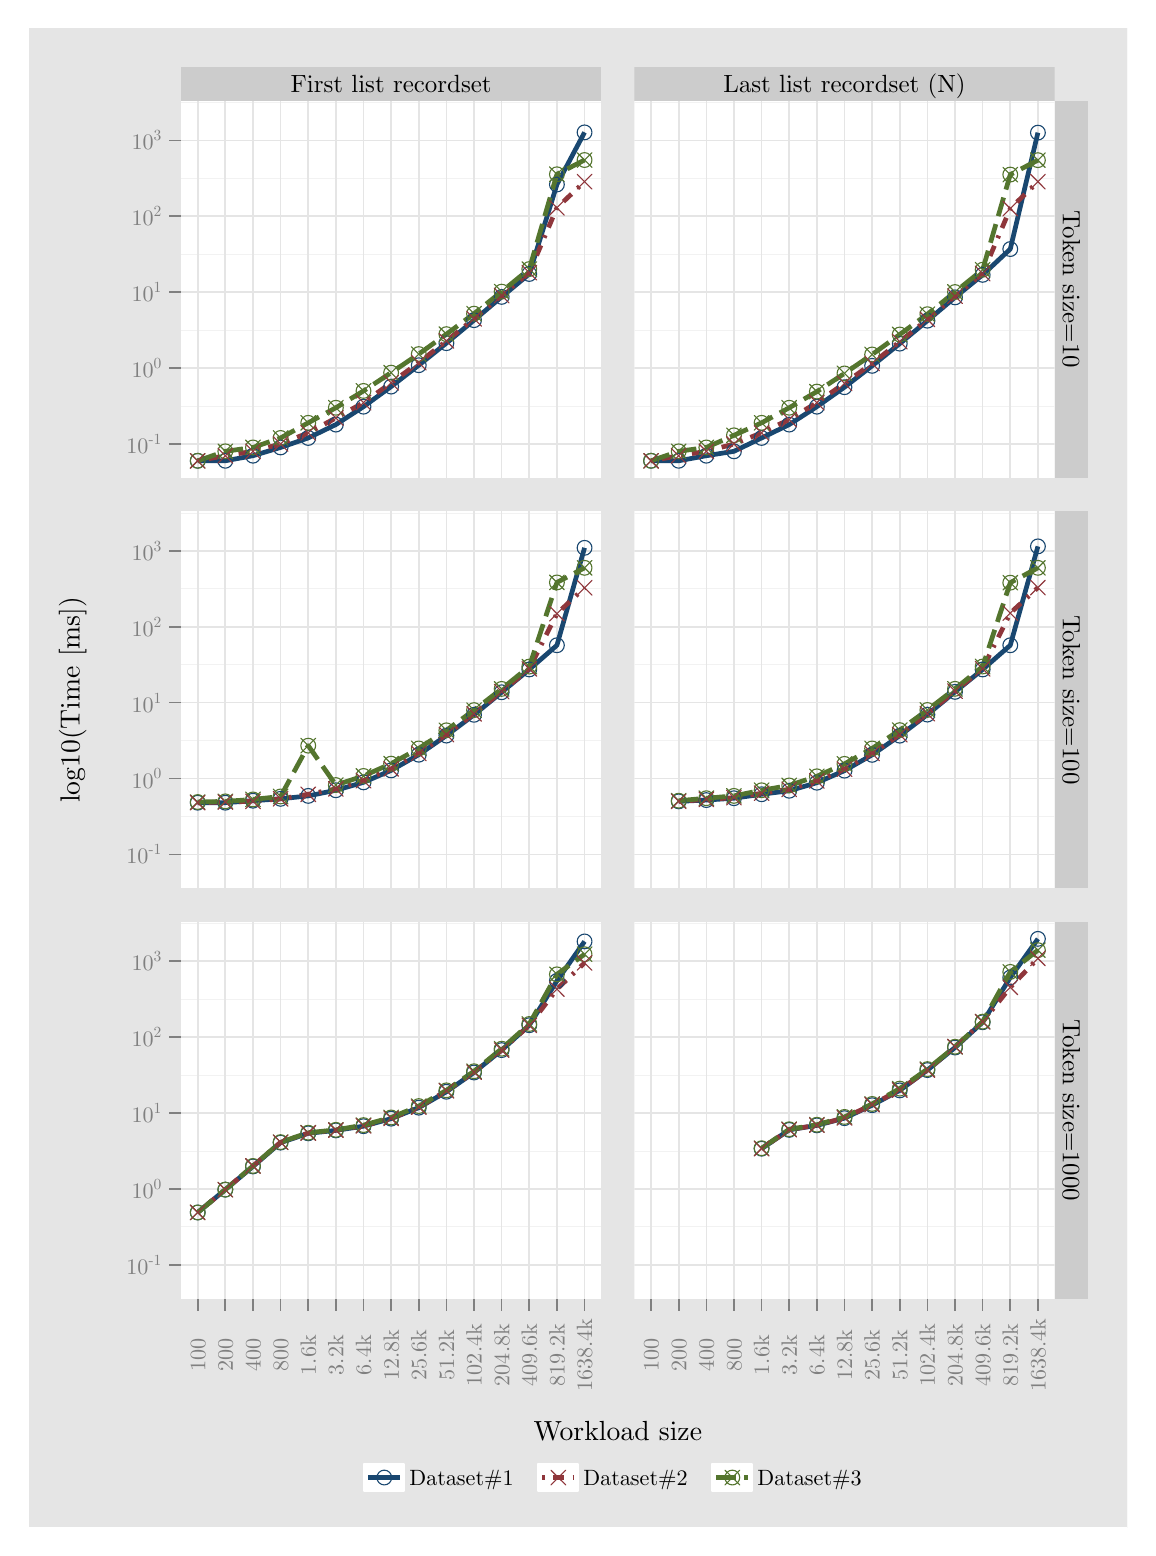
\begin{tikzpicture}[x=1pt,y=1pt]
\definecolor[named]{fillColor}{rgb}{1.00,1.00,1.00}
\path[use as bounding box,fill=fillColor,fill opacity=0.00] (0,0) rectangle (397.48,542.02);
\begin{scope}
\path[clip] (  0.00,  0.00) rectangle (397.48,542.02);
\definecolor[named]{drawColor}{rgb}{1.00,1.00,1.00}
\definecolor[named]{fillColor}{rgb}{0.90,0.90,0.90}

\path[draw=drawColor,line width= 0.6pt,line join=round,line cap=round,fill=fillColor] (  0.00,  0.00) rectangle (397.48,542.02);
\end{scope}
\begin{scope}
\path[clip] ( 55.45,515.58) rectangle (207.22,527.80);
\definecolor[named]{fillColor}{rgb}{0.80,0.80,0.80}

\path[fill=fillColor] ( 55.45,515.58) rectangle (207.22,527.80);
\definecolor[named]{drawColor}{rgb}{0.00,0.00,0.00}

\node[text=drawColor,anchor=base,inner sep=0pt, outer sep=0pt, scale=  0.90] at (131.33,518.59) {First list recordset };
\end{scope}
\begin{scope}
\path[clip] (219.27,515.58) rectangle (371.04,527.80);
\definecolor[named]{fillColor}{rgb}{0.80,0.80,0.80}

\path[fill=fillColor] (219.27,515.58) rectangle (371.04,527.80);
\definecolor[named]{drawColor}{rgb}{0.00,0.00,0.00}

\node[text=drawColor,anchor=base,inner sep=0pt, outer sep=0pt, scale=  0.90] at (295.15,518.59) {Last list recordset (N) };
\end{scope}
\begin{scope}
\path[clip] ( 55.45,379.31) rectangle (207.22,515.58);
\definecolor[named]{fillColor}{rgb}{1.00,1.00,1.00}

\path[fill=fillColor] ( 55.45,379.31) rectangle (207.22,515.58);
\definecolor[named]{drawColor}{rgb}{0.95,0.95,0.95}

\path[draw=drawColor,line width= 0.3pt,line join=round] ( 55.45,405.30) --
	(207.22,405.30);

\path[draw=drawColor,line width= 0.3pt,line join=round] ( 55.45,432.72) --
	(207.22,432.72);

\path[draw=drawColor,line width= 0.3pt,line join=round] ( 55.45,460.14) --
	(207.22,460.14);

\path[draw=drawColor,line width= 0.3pt,line join=round] ( 55.45,487.56) --
	(207.22,487.56);

\path[draw=drawColor,line width= 0.3pt,line join=round] ( 55.45,514.98) --
	(207.22,514.98);
\definecolor[named]{drawColor}{rgb}{0.90,0.90,0.90}

\path[draw=drawColor,line width= 0.6pt,line join=round] ( 55.45,391.59) --
	(207.22,391.59);

\path[draw=drawColor,line width= 0.6pt,line join=round] ( 55.45,419.01) --
	(207.22,419.01);

\path[draw=drawColor,line width= 0.6pt,line join=round] ( 55.45,446.43) --
	(207.22,446.43);

\path[draw=drawColor,line width= 0.6pt,line join=round] ( 55.45,473.85) --
	(207.22,473.85);

\path[draw=drawColor,line width= 0.6pt,line join=round] ( 55.45,501.27) --
	(207.22,501.27);

\path[draw=drawColor,line width= 0.6pt,line join=round] ( 61.44,379.31) --
	( 61.44,515.58);

\path[draw=drawColor,line width= 0.6pt,line join=round] ( 71.42,379.31) --
	( 71.42,515.58);

\path[draw=drawColor,line width= 0.6pt,line join=round] ( 81.41,379.31) --
	( 81.41,515.58);

\path[draw=drawColor,line width= 0.6pt,line join=round] ( 91.39,379.31) --
	( 91.39,515.58);

\path[draw=drawColor,line width= 0.6pt,line join=round] (101.38,379.31) --
	(101.38,515.58);

\path[draw=drawColor,line width= 0.6pt,line join=round] (111.36,379.31) --
	(111.36,515.58);

\path[draw=drawColor,line width= 0.6pt,line join=round] (121.35,379.31) --
	(121.35,515.58);

\path[draw=drawColor,line width= 0.6pt,line join=round] (131.33,379.31) --
	(131.33,515.58);

\path[draw=drawColor,line width= 0.6pt,line join=round] (141.32,379.31) --
	(141.32,515.58);

\path[draw=drawColor,line width= 0.6pt,line join=round] (151.30,379.31) --
	(151.30,515.58);

\path[draw=drawColor,line width= 0.6pt,line join=round] (161.29,379.31) --
	(161.29,515.58);

\path[draw=drawColor,line width= 0.6pt,line join=round] (171.27,379.31) --
	(171.27,515.58);

\path[draw=drawColor,line width= 0.6pt,line join=round] (181.26,379.31) --
	(181.26,515.58);

\path[draw=drawColor,line width= 0.6pt,line join=round] (191.24,379.31) --
	(191.24,515.58);

\path[draw=drawColor,line width= 0.6pt,line join=round] (201.23,379.31) --
	(201.23,515.58);
\definecolor[named]{drawColor}{rgb}{0.10,0.28,0.44}

\path[draw=drawColor,line width= 1.7pt,line join=round] ( 61.44,385.51) --
	( 71.42,385.51) --
	( 81.41,387.34) --
	( 91.39,390.33) --
	(101.38,393.76) --
	(111.36,398.59) --
	(121.35,405.06) --
	(131.33,412.32) --
	(141.32,420.04) --
	(151.30,428.01) --
	(161.29,436.32) --
	(171.27,444.74) --
	(181.26,453.01) --
	(191.24,485.34) --
	(201.23,504.18);
\definecolor[named]{drawColor}{rgb}{0.56,0.21,0.23}

\path[draw=drawColor,line width= 1.7pt,dash pattern=on 1pt off 3pt on 4pt off 3pt ,line join=round] ( 61.44,385.51) --
	( 71.42,387.34) --
	( 81.41,388.93) --
	( 91.39,391.59) --
	(101.38,395.60) --
	(111.36,400.98) --
	(121.35,406.51) --
	(131.33,413.69) --
	(141.32,420.98) --
	(151.30,428.82) --
	(161.29,436.84) --
	(171.27,445.24) --
	(181.26,453.48) --
	(191.24,476.93) --
	(201.23,486.38);
\definecolor[named]{drawColor}{rgb}{0.33,0.46,0.18}

\path[draw=drawColor,line width= 1.7pt,dash pattern=on 7pt off 3pt ,line join=round] ( 61.44,385.51) --
	( 71.42,388.93) --
	( 81.41,390.33) --
	( 91.39,393.76) --
	(101.38,399.23) --
	(111.36,404.67) --
	(121.35,410.75) --
	(131.33,417.35) --
	(141.32,424.07) --
	(151.30,431.27) --
	(161.29,438.67) --
	(171.27,446.63) --
	(181.26,454.79) --
	(191.24,489.04) --
	(201.23,494.19);
\definecolor[named]{drawColor}{rgb}{0.10,0.28,0.44}

\path[draw=drawColor,line width= 0.4pt,line join=round,line cap=round] ( 61.44,385.51) circle (  2.67);

\path[draw=drawColor,line width= 0.4pt,line join=round,line cap=round] ( 71.42,385.51) circle (  2.67);

\path[draw=drawColor,line width= 0.4pt,line join=round,line cap=round] ( 81.41,387.34) circle (  2.67);

\path[draw=drawColor,line width= 0.4pt,line join=round,line cap=round] ( 91.39,390.33) circle (  2.67);

\path[draw=drawColor,line width= 0.4pt,line join=round,line cap=round] (101.38,393.76) circle (  2.67);

\path[draw=drawColor,line width= 0.4pt,line join=round,line cap=round] (111.36,398.59) circle (  2.67);

\path[draw=drawColor,line width= 0.4pt,line join=round,line cap=round] (121.35,405.06) circle (  2.67);

\path[draw=drawColor,line width= 0.4pt,line join=round,line cap=round] (131.33,412.32) circle (  2.67);

\path[draw=drawColor,line width= 0.4pt,line join=round,line cap=round] (141.32,420.04) circle (  2.67);

\path[draw=drawColor,line width= 0.4pt,line join=round,line cap=round] (151.30,428.01) circle (  2.67);

\path[draw=drawColor,line width= 0.4pt,line join=round,line cap=round] (161.29,436.32) circle (  2.67);

\path[draw=drawColor,line width= 0.4pt,line join=round,line cap=round] (171.27,444.74) circle (  2.67);

\path[draw=drawColor,line width= 0.4pt,line join=round,line cap=round] (181.26,453.01) circle (  2.67);

\path[draw=drawColor,line width= 0.4pt,line join=round,line cap=round] (191.24,485.34) circle (  2.67);

\path[draw=drawColor,line width= 0.4pt,line join=round,line cap=round] (201.23,504.18) circle (  2.67);
\definecolor[named]{drawColor}{rgb}{0.33,0.46,0.18}

\path[draw=drawColor,line width= 0.4pt,line join=round,line cap=round] ( 61.44,385.51) circle (  2.67);

\path[draw=drawColor,line width= 0.4pt,line join=round,line cap=round] ( 58.77,382.84) -- ( 64.11,388.17);

\path[draw=drawColor,line width= 0.4pt,line join=round,line cap=round] ( 58.77,388.17) -- ( 64.11,382.84);

\path[draw=drawColor,line width= 0.4pt,line join=round,line cap=round] ( 71.42,388.93) circle (  2.67);

\path[draw=drawColor,line width= 0.4pt,line join=round,line cap=round] ( 68.76,386.26) -- ( 74.09,391.60);

\path[draw=drawColor,line width= 0.4pt,line join=round,line cap=round] ( 68.76,391.60) -- ( 74.09,386.26);

\path[draw=drawColor,line width= 0.4pt,line join=round,line cap=round] ( 81.41,390.33) circle (  2.67);

\path[draw=drawColor,line width= 0.4pt,line join=round,line cap=round] ( 78.74,387.67) -- ( 84.08,393.00);

\path[draw=drawColor,line width= 0.4pt,line join=round,line cap=round] ( 78.74,393.00) -- ( 84.08,387.67);

\path[draw=drawColor,line width= 0.4pt,line join=round,line cap=round] ( 91.39,393.76) circle (  2.67);

\path[draw=drawColor,line width= 0.4pt,line join=round,line cap=round] ( 88.73,391.09) -- ( 94.06,396.43);

\path[draw=drawColor,line width= 0.4pt,line join=round,line cap=round] ( 88.73,396.43) -- ( 94.06,391.09);

\path[draw=drawColor,line width= 0.4pt,line join=round,line cap=round] (101.38,399.23) circle (  2.67);

\path[draw=drawColor,line width= 0.4pt,line join=round,line cap=round] ( 98.71,396.57) -- (104.05,401.90);

\path[draw=drawColor,line width= 0.4pt,line join=round,line cap=round] ( 98.71,401.90) -- (104.05,396.57);

\path[draw=drawColor,line width= 0.4pt,line join=round,line cap=round] (111.36,404.67) circle (  2.67);

\path[draw=drawColor,line width= 0.4pt,line join=round,line cap=round] (108.70,402.00) -- (114.03,407.34);

\path[draw=drawColor,line width= 0.4pt,line join=round,line cap=round] (108.70,407.34) -- (114.03,402.00);

\path[draw=drawColor,line width= 0.4pt,line join=round,line cap=round] (121.35,410.75) circle (  2.67);

\path[draw=drawColor,line width= 0.4pt,line join=round,line cap=round] (118.68,408.09) -- (124.02,413.42);

\path[draw=drawColor,line width= 0.4pt,line join=round,line cap=round] (118.68,413.42) -- (124.02,408.09);

\path[draw=drawColor,line width= 0.4pt,line join=round,line cap=round] (131.33,417.35) circle (  2.67);

\path[draw=drawColor,line width= 0.4pt,line join=round,line cap=round] (128.67,414.68) -- (134.00,420.02);

\path[draw=drawColor,line width= 0.4pt,line join=round,line cap=round] (128.67,420.02) -- (134.00,414.68);

\path[draw=drawColor,line width= 0.4pt,line join=round,line cap=round] (141.32,424.07) circle (  2.67);

\path[draw=drawColor,line width= 0.4pt,line join=round,line cap=round] (138.65,421.41) -- (143.99,426.74);

\path[draw=drawColor,line width= 0.4pt,line join=round,line cap=round] (138.65,426.74) -- (143.99,421.41);

\path[draw=drawColor,line width= 0.4pt,line join=round,line cap=round] (151.30,431.27) circle (  2.67);

\path[draw=drawColor,line width= 0.4pt,line join=round,line cap=round] (148.64,428.60) -- (153.97,433.94);

\path[draw=drawColor,line width= 0.4pt,line join=round,line cap=round] (148.64,433.94) -- (153.97,428.60);

\path[draw=drawColor,line width= 0.4pt,line join=round,line cap=round] (161.29,438.67) circle (  2.67);

\path[draw=drawColor,line width= 0.4pt,line join=round,line cap=round] (158.62,436.00) -- (163.96,441.33);

\path[draw=drawColor,line width= 0.4pt,line join=round,line cap=round] (158.62,441.33) -- (163.96,436.00);

\path[draw=drawColor,line width= 0.4pt,line join=round,line cap=round] (171.27,446.63) circle (  2.67);

\path[draw=drawColor,line width= 0.4pt,line join=round,line cap=round] (168.61,443.96) -- (173.94,449.30);

\path[draw=drawColor,line width= 0.4pt,line join=round,line cap=round] (168.61,449.30) -- (173.94,443.96);

\path[draw=drawColor,line width= 0.4pt,line join=round,line cap=round] (181.26,454.79) circle (  2.67);

\path[draw=drawColor,line width= 0.4pt,line join=round,line cap=round] (178.59,452.12) -- (183.93,457.46);

\path[draw=drawColor,line width= 0.4pt,line join=round,line cap=round] (178.59,457.46) -- (183.93,452.12);

\path[draw=drawColor,line width= 0.4pt,line join=round,line cap=round] (191.24,489.04) circle (  2.67);

\path[draw=drawColor,line width= 0.4pt,line join=round,line cap=round] (188.58,486.37) -- (193.91,491.71);

\path[draw=drawColor,line width= 0.4pt,line join=round,line cap=round] (188.58,491.71) -- (193.91,486.37);

\path[draw=drawColor,line width= 0.4pt,line join=round,line cap=round] (201.23,494.19) circle (  2.67);

\path[draw=drawColor,line width= 0.4pt,line join=round,line cap=round] (198.56,491.52) -- (203.90,496.85);

\path[draw=drawColor,line width= 0.4pt,line join=round,line cap=round] (198.56,496.85) -- (203.90,491.52);
\definecolor[named]{drawColor}{rgb}{0.56,0.21,0.23}

\path[draw=drawColor,line width= 0.4pt,line join=round,line cap=round,fill=fillColor] ( 58.77,382.84) -- ( 64.11,388.17);

\path[draw=drawColor,line width= 0.4pt,line join=round,line cap=round,fill=fillColor] ( 58.77,388.17) -- ( 64.11,382.84);

\path[draw=drawColor,line width= 0.4pt,line join=round,line cap=round,fill=fillColor] ( 68.76,384.67) -- ( 74.09,390.01);

\path[draw=drawColor,line width= 0.4pt,line join=round,line cap=round,fill=fillColor] ( 68.76,390.01) -- ( 74.09,384.67);

\path[draw=drawColor,line width= 0.4pt,line join=round,line cap=round,fill=fillColor] ( 78.74,386.26) -- ( 84.08,391.60);

\path[draw=drawColor,line width= 0.4pt,line join=round,line cap=round,fill=fillColor] ( 78.74,391.60) -- ( 84.08,386.26);

\path[draw=drawColor,line width= 0.4pt,line join=round,line cap=round,fill=fillColor] ( 88.73,388.92) -- ( 94.06,394.26);

\path[draw=drawColor,line width= 0.4pt,line join=round,line cap=round,fill=fillColor] ( 88.73,394.26) -- ( 94.06,388.92);

\path[draw=drawColor,line width= 0.4pt,line join=round,line cap=round,fill=fillColor] ( 98.71,392.93) -- (104.05,398.26);

\path[draw=drawColor,line width= 0.4pt,line join=round,line cap=round,fill=fillColor] ( 98.71,398.26) -- (104.05,392.93);

\path[draw=drawColor,line width= 0.4pt,line join=round,line cap=round,fill=fillColor] (108.70,398.31) -- (114.03,403.65);

\path[draw=drawColor,line width= 0.4pt,line join=round,line cap=round,fill=fillColor] (108.70,403.65) -- (114.03,398.31);

\path[draw=drawColor,line width= 0.4pt,line join=round,line cap=round,fill=fillColor] (118.68,403.84) -- (124.02,409.17);

\path[draw=drawColor,line width= 0.4pt,line join=round,line cap=round,fill=fillColor] (118.68,409.17) -- (124.02,403.84);

\path[draw=drawColor,line width= 0.4pt,line join=round,line cap=round,fill=fillColor] (128.67,411.03) -- (134.00,416.36);

\path[draw=drawColor,line width= 0.4pt,line join=round,line cap=round,fill=fillColor] (128.67,416.36) -- (134.00,411.03);

\path[draw=drawColor,line width= 0.4pt,line join=round,line cap=round,fill=fillColor] (138.65,418.31) -- (143.99,423.65);

\path[draw=drawColor,line width= 0.4pt,line join=round,line cap=round,fill=fillColor] (138.65,423.65) -- (143.99,418.31);

\path[draw=drawColor,line width= 0.4pt,line join=round,line cap=round,fill=fillColor] (148.64,426.16) -- (153.97,431.49);

\path[draw=drawColor,line width= 0.4pt,line join=round,line cap=round,fill=fillColor] (148.64,431.49) -- (153.97,426.16);

\path[draw=drawColor,line width= 0.4pt,line join=round,line cap=round,fill=fillColor] (158.62,434.17) -- (163.96,439.51);

\path[draw=drawColor,line width= 0.4pt,line join=round,line cap=round,fill=fillColor] (158.62,439.51) -- (163.96,434.17);

\path[draw=drawColor,line width= 0.4pt,line join=round,line cap=round,fill=fillColor] (168.61,442.57) -- (173.94,447.91);

\path[draw=drawColor,line width= 0.4pt,line join=round,line cap=round,fill=fillColor] (168.61,447.91) -- (173.94,442.57);

\path[draw=drawColor,line width= 0.4pt,line join=round,line cap=round,fill=fillColor] (178.59,450.81) -- (183.93,456.14);

\path[draw=drawColor,line width= 0.4pt,line join=round,line cap=round,fill=fillColor] (178.59,456.14) -- (183.93,450.81);

\path[draw=drawColor,line width= 0.4pt,line join=round,line cap=round,fill=fillColor] (188.58,474.26) -- (193.91,479.60);

\path[draw=drawColor,line width= 0.4pt,line join=round,line cap=round,fill=fillColor] (188.58,479.60) -- (193.91,474.26);

\path[draw=drawColor,line width= 0.4pt,line join=round,line cap=round,fill=fillColor] (198.56,483.72) -- (203.90,489.05);

\path[draw=drawColor,line width= 0.4pt,line join=round,line cap=round,fill=fillColor] (198.56,489.05) -- (203.90,483.72);
\end{scope}
\begin{scope}
\path[clip] ( 55.45,231.00) rectangle (207.22,367.27);
\definecolor[named]{fillColor}{rgb}{1.00,1.00,1.00}

\path[fill=fillColor] ( 55.45,231.00) rectangle (207.22,367.27);
\definecolor[named]{drawColor}{rgb}{0.95,0.95,0.95}

\path[draw=drawColor,line width= 0.3pt,line join=round] ( 55.45,256.99) --
	(207.22,256.99);

\path[draw=drawColor,line width= 0.3pt,line join=round] ( 55.45,284.41) --
	(207.22,284.41);

\path[draw=drawColor,line width= 0.3pt,line join=round] ( 55.45,311.83) --
	(207.22,311.83);

\path[draw=drawColor,line width= 0.3pt,line join=round] ( 55.45,339.25) --
	(207.22,339.25);

\path[draw=drawColor,line width= 0.3pt,line join=round] ( 55.45,366.67) --
	(207.22,366.67);
\definecolor[named]{drawColor}{rgb}{0.90,0.90,0.90}

\path[draw=drawColor,line width= 0.6pt,line join=round] ( 55.45,243.28) --
	(207.22,243.28);

\path[draw=drawColor,line width= 0.6pt,line join=round] ( 55.45,270.70) --
	(207.22,270.70);

\path[draw=drawColor,line width= 0.6pt,line join=round] ( 55.45,298.12) --
	(207.22,298.12);

\path[draw=drawColor,line width= 0.6pt,line join=round] ( 55.45,325.54) --
	(207.22,325.54);

\path[draw=drawColor,line width= 0.6pt,line join=round] ( 55.45,352.96) --
	(207.22,352.96);

\path[draw=drawColor,line width= 0.6pt,line join=round] ( 61.44,231.00) --
	( 61.44,367.27);

\path[draw=drawColor,line width= 0.6pt,line join=round] ( 71.42,231.00) --
	( 71.42,367.27);

\path[draw=drawColor,line width= 0.6pt,line join=round] ( 81.41,231.00) --
	( 81.41,367.27);

\path[draw=drawColor,line width= 0.6pt,line join=round] ( 91.39,231.00) --
	( 91.39,367.27);

\path[draw=drawColor,line width= 0.6pt,line join=round] (101.38,231.00) --
	(101.38,367.27);

\path[draw=drawColor,line width= 0.6pt,line join=round] (111.36,231.00) --
	(111.36,367.27);

\path[draw=drawColor,line width= 0.6pt,line join=round] (121.35,231.00) --
	(121.35,367.27);

\path[draw=drawColor,line width= 0.6pt,line join=round] (131.33,231.00) --
	(131.33,367.27);

\path[draw=drawColor,line width= 0.6pt,line join=round] (141.32,231.00) --
	(141.32,367.27);

\path[draw=drawColor,line width= 0.6pt,line join=round] (151.30,231.00) --
	(151.30,367.27);

\path[draw=drawColor,line width= 0.6pt,line join=round] (161.29,231.00) --
	(161.29,367.27);

\path[draw=drawColor,line width= 0.6pt,line join=round] (171.27,231.00) --
	(171.27,367.27);

\path[draw=drawColor,line width= 0.6pt,line join=round] (181.26,231.00) --
	(181.26,367.27);

\path[draw=drawColor,line width= 0.6pt,line join=round] (191.24,231.00) --
	(191.24,367.27);

\path[draw=drawColor,line width= 0.6pt,line join=round] (201.23,231.00) --
	(201.23,367.27);
\definecolor[named]{drawColor}{rgb}{0.10,0.28,0.44}

\path[draw=drawColor,line width= 1.7pt,line join=round] ( 61.44,261.96) --
	( 71.42,261.96) --
	( 81.41,262.68) --
	( 91.39,263.36) --
	(101.38,264.42) --
	(111.36,266.45) --
	(121.35,269.31) --
	(131.33,273.64) --
	(141.32,279.30) --
	(151.30,286.21) --
	(161.29,293.72) --
	(171.27,301.87) --
	(181.26,310.12) --
	(191.24,318.85) --
	(201.23,354.06);
\definecolor[named]{drawColor}{rgb}{0.56,0.21,0.23}

\path[draw=drawColor,line width= 1.7pt,dash pattern=on 1pt off 3pt on 4pt off 3pt ,line join=round] ( 61.44,261.96) --
	( 71.42,262.20) --
	( 81.41,262.44) --
	( 91.39,263.36) --
	(101.38,265.01) --
	(111.36,266.95) --
	(121.35,269.96) --
	(131.33,274.18) --
	(141.32,279.76) --
	(151.30,286.57) --
	(161.29,294.09) --
	(171.27,302.12) --
	(181.26,310.33) --
	(191.24,330.27) --
	(201.23,339.63);
\definecolor[named]{drawColor}{rgb}{0.33,0.46,0.18}

\path[draw=drawColor,line width= 1.7pt,dash pattern=on 7pt off 3pt ,line join=round] ( 61.44,262.20) --
	( 71.42,262.44) --
	( 81.41,263.14) --
	( 91.39,264.21) --
	(101.38,282.57) --
	(111.36,268.34) --
	(121.35,271.62) --
	(131.33,276.07) --
	(141.32,281.56) --
	(151.30,288.12) --
	(161.29,295.42) --
	(171.27,303.08) --
	(181.26,311.15) --
	(191.24,341.55) --
	(201.23,346.83);
\definecolor[named]{drawColor}{rgb}{0.10,0.28,0.44}

\path[draw=drawColor,line width= 0.4pt,line join=round,line cap=round] ( 61.44,261.96) circle (  2.67);

\path[draw=drawColor,line width= 0.4pt,line join=round,line cap=round] ( 71.42,261.96) circle (  2.67);

\path[draw=drawColor,line width= 0.4pt,line join=round,line cap=round] ( 81.41,262.68) circle (  2.67);

\path[draw=drawColor,line width= 0.4pt,line join=round,line cap=round] ( 91.39,263.36) circle (  2.67);

\path[draw=drawColor,line width= 0.4pt,line join=round,line cap=round] (101.38,264.42) circle (  2.67);

\path[draw=drawColor,line width= 0.4pt,line join=round,line cap=round] (111.36,266.45) circle (  2.67);

\path[draw=drawColor,line width= 0.4pt,line join=round,line cap=round] (121.35,269.31) circle (  2.67);

\path[draw=drawColor,line width= 0.4pt,line join=round,line cap=round] (131.33,273.64) circle (  2.67);

\path[draw=drawColor,line width= 0.4pt,line join=round,line cap=round] (141.32,279.30) circle (  2.67);

\path[draw=drawColor,line width= 0.4pt,line join=round,line cap=round] (151.30,286.21) circle (  2.67);

\path[draw=drawColor,line width= 0.4pt,line join=round,line cap=round] (161.29,293.72) circle (  2.67);

\path[draw=drawColor,line width= 0.4pt,line join=round,line cap=round] (171.27,301.87) circle (  2.67);

\path[draw=drawColor,line width= 0.4pt,line join=round,line cap=round] (181.26,310.12) circle (  2.67);

\path[draw=drawColor,line width= 0.4pt,line join=round,line cap=round] (191.24,318.85) circle (  2.67);

\path[draw=drawColor,line width= 0.4pt,line join=round,line cap=round] (201.23,354.06) circle (  2.67);
\definecolor[named]{drawColor}{rgb}{0.33,0.46,0.18}

\path[draw=drawColor,line width= 0.4pt,line join=round,line cap=round] ( 61.44,262.20) circle (  2.67);

\path[draw=drawColor,line width= 0.4pt,line join=round,line cap=round] ( 58.77,259.54) -- ( 64.11,264.87);

\path[draw=drawColor,line width= 0.4pt,line join=round,line cap=round] ( 58.77,264.87) -- ( 64.11,259.54);

\path[draw=drawColor,line width= 0.4pt,line join=round,line cap=round] ( 71.42,262.44) circle (  2.67);

\path[draw=drawColor,line width= 0.4pt,line join=round,line cap=round] ( 68.76,259.78) -- ( 74.09,265.11);

\path[draw=drawColor,line width= 0.4pt,line join=round,line cap=round] ( 68.76,265.11) -- ( 74.09,259.78);

\path[draw=drawColor,line width= 0.4pt,line join=round,line cap=round] ( 81.41,263.14) circle (  2.67);

\path[draw=drawColor,line width= 0.4pt,line join=round,line cap=round] ( 78.74,260.47) -- ( 84.08,265.81);

\path[draw=drawColor,line width= 0.4pt,line join=round,line cap=round] ( 78.74,265.81) -- ( 84.08,260.47);

\path[draw=drawColor,line width= 0.4pt,line join=round,line cap=round] ( 91.39,264.21) circle (  2.67);

\path[draw=drawColor,line width= 0.4pt,line join=round,line cap=round] ( 88.73,261.54) -- ( 94.06,266.88);

\path[draw=drawColor,line width= 0.4pt,line join=round,line cap=round] ( 88.73,266.88) -- ( 94.06,261.54);

\path[draw=drawColor,line width= 0.4pt,line join=round,line cap=round] (101.38,282.57) circle (  2.67);

\path[draw=drawColor,line width= 0.4pt,line join=round,line cap=round] ( 98.71,279.90) -- (104.05,285.24);

\path[draw=drawColor,line width= 0.4pt,line join=round,line cap=round] ( 98.71,285.24) -- (104.05,279.90);

\path[draw=drawColor,line width= 0.4pt,line join=round,line cap=round] (111.36,268.34) circle (  2.67);

\path[draw=drawColor,line width= 0.4pt,line join=round,line cap=round] (108.70,265.67) -- (114.03,271.00);

\path[draw=drawColor,line width= 0.4pt,line join=round,line cap=round] (108.70,271.00) -- (114.03,265.67);

\path[draw=drawColor,line width= 0.4pt,line join=round,line cap=round] (121.35,271.62) circle (  2.67);

\path[draw=drawColor,line width= 0.4pt,line join=round,line cap=round] (118.68,268.95) -- (124.02,274.28);

\path[draw=drawColor,line width= 0.4pt,line join=round,line cap=round] (118.68,274.28) -- (124.02,268.95);

\path[draw=drawColor,line width= 0.4pt,line join=round,line cap=round] (131.33,276.07) circle (  2.67);

\path[draw=drawColor,line width= 0.4pt,line join=round,line cap=round] (128.67,273.40) -- (134.00,278.74);

\path[draw=drawColor,line width= 0.4pt,line join=round,line cap=round] (128.67,278.74) -- (134.00,273.40);

\path[draw=drawColor,line width= 0.4pt,line join=round,line cap=round] (141.32,281.56) circle (  2.67);

\path[draw=drawColor,line width= 0.4pt,line join=round,line cap=round] (138.65,278.90) -- (143.99,284.23);

\path[draw=drawColor,line width= 0.4pt,line join=round,line cap=round] (138.65,284.23) -- (143.99,278.90);

\path[draw=drawColor,line width= 0.4pt,line join=round,line cap=round] (151.30,288.12) circle (  2.67);

\path[draw=drawColor,line width= 0.4pt,line join=round,line cap=round] (148.64,285.46) -- (153.97,290.79);

\path[draw=drawColor,line width= 0.4pt,line join=round,line cap=round] (148.64,290.79) -- (153.97,285.46);

\path[draw=drawColor,line width= 0.4pt,line join=round,line cap=round] (161.29,295.42) circle (  2.67);

\path[draw=drawColor,line width= 0.4pt,line join=round,line cap=round] (158.62,292.75) -- (163.96,298.08);

\path[draw=drawColor,line width= 0.4pt,line join=round,line cap=round] (158.62,298.08) -- (163.96,292.75);

\path[draw=drawColor,line width= 0.4pt,line join=round,line cap=round] (171.27,303.08) circle (  2.67);

\path[draw=drawColor,line width= 0.4pt,line join=round,line cap=round] (168.61,300.41) -- (173.94,305.75);

\path[draw=drawColor,line width= 0.4pt,line join=round,line cap=round] (168.61,305.75) -- (173.94,300.41);

\path[draw=drawColor,line width= 0.4pt,line join=round,line cap=round] (181.26,311.15) circle (  2.67);

\path[draw=drawColor,line width= 0.4pt,line join=round,line cap=round] (178.59,308.49) -- (183.93,313.82);

\path[draw=drawColor,line width= 0.4pt,line join=round,line cap=round] (178.59,313.82) -- (183.93,308.49);

\path[draw=drawColor,line width= 0.4pt,line join=round,line cap=round] (191.24,341.55) circle (  2.67);

\path[draw=drawColor,line width= 0.4pt,line join=round,line cap=round] (188.58,338.89) -- (193.91,344.22);

\path[draw=drawColor,line width= 0.4pt,line join=round,line cap=round] (188.58,344.22) -- (193.91,338.89);

\path[draw=drawColor,line width= 0.4pt,line join=round,line cap=round] (201.23,346.83) circle (  2.67);

\path[draw=drawColor,line width= 0.4pt,line join=round,line cap=round] (198.56,344.16) -- (203.90,349.49);

\path[draw=drawColor,line width= 0.4pt,line join=round,line cap=round] (198.56,349.49) -- (203.90,344.16);
\definecolor[named]{drawColor}{rgb}{0.56,0.21,0.23}

\path[draw=drawColor,line width= 0.4pt,line join=round,line cap=round,fill=fillColor] ( 58.77,259.29) -- ( 64.11,264.63);

\path[draw=drawColor,line width= 0.4pt,line join=round,line cap=round,fill=fillColor] ( 58.77,264.63) -- ( 64.11,259.29);

\path[draw=drawColor,line width= 0.4pt,line join=round,line cap=round,fill=fillColor] ( 68.76,259.54) -- ( 74.09,264.87);

\path[draw=drawColor,line width= 0.4pt,line join=round,line cap=round,fill=fillColor] ( 68.76,264.87) -- ( 74.09,259.54);

\path[draw=drawColor,line width= 0.4pt,line join=round,line cap=round,fill=fillColor] ( 78.74,259.78) -- ( 84.08,265.11);

\path[draw=drawColor,line width= 0.4pt,line join=round,line cap=round,fill=fillColor] ( 78.74,265.11) -- ( 84.08,259.78);

\path[draw=drawColor,line width= 0.4pt,line join=round,line cap=round,fill=fillColor] ( 88.73,260.69) -- ( 94.06,266.03);

\path[draw=drawColor,line width= 0.4pt,line join=round,line cap=round,fill=fillColor] ( 88.73,266.03) -- ( 94.06,260.69);

\path[draw=drawColor,line width= 0.4pt,line join=round,line cap=round,fill=fillColor] ( 98.71,262.34) -- (104.05,267.67);

\path[draw=drawColor,line width= 0.4pt,line join=round,line cap=round,fill=fillColor] ( 98.71,267.67) -- (104.05,262.34);

\path[draw=drawColor,line width= 0.4pt,line join=round,line cap=round,fill=fillColor] (108.70,264.28) -- (114.03,269.62);

\path[draw=drawColor,line width= 0.4pt,line join=round,line cap=round,fill=fillColor] (108.70,269.62) -- (114.03,264.28);

\path[draw=drawColor,line width= 0.4pt,line join=round,line cap=round,fill=fillColor] (118.68,267.29) -- (124.02,272.63);

\path[draw=drawColor,line width= 0.4pt,line join=round,line cap=round,fill=fillColor] (118.68,272.63) -- (124.02,267.29);

\path[draw=drawColor,line width= 0.4pt,line join=round,line cap=round,fill=fillColor] (128.67,271.52) -- (134.00,276.85);

\path[draw=drawColor,line width= 0.4pt,line join=round,line cap=round,fill=fillColor] (128.67,276.85) -- (134.00,271.52);

\path[draw=drawColor,line width= 0.4pt,line join=round,line cap=round,fill=fillColor] (138.65,277.09) -- (143.99,282.43);

\path[draw=drawColor,line width= 0.4pt,line join=round,line cap=round,fill=fillColor] (138.65,282.43) -- (143.99,277.09);

\path[draw=drawColor,line width= 0.4pt,line join=round,line cap=round,fill=fillColor] (148.64,283.90) -- (153.97,289.23);

\path[draw=drawColor,line width= 0.4pt,line join=round,line cap=round,fill=fillColor] (148.64,289.23) -- (153.97,283.90);

\path[draw=drawColor,line width= 0.4pt,line join=round,line cap=round,fill=fillColor] (158.62,291.42) -- (163.96,296.76);

\path[draw=drawColor,line width= 0.4pt,line join=round,line cap=round,fill=fillColor] (158.62,296.76) -- (163.96,291.42);

\path[draw=drawColor,line width= 0.4pt,line join=round,line cap=round,fill=fillColor] (168.61,299.45) -- (173.94,304.78);

\path[draw=drawColor,line width= 0.4pt,line join=round,line cap=round,fill=fillColor] (168.61,304.78) -- (173.94,299.45);

\path[draw=drawColor,line width= 0.4pt,line join=round,line cap=round,fill=fillColor] (178.59,307.67) -- (183.93,313.00);

\path[draw=drawColor,line width= 0.4pt,line join=round,line cap=round,fill=fillColor] (178.59,313.00) -- (183.93,307.67);

\path[draw=drawColor,line width= 0.4pt,line join=round,line cap=round,fill=fillColor] (188.58,327.60) -- (193.91,332.94);

\path[draw=drawColor,line width= 0.4pt,line join=round,line cap=round,fill=fillColor] (188.58,332.94) -- (193.91,327.60);

\path[draw=drawColor,line width= 0.4pt,line join=round,line cap=round,fill=fillColor] (198.56,336.96) -- (203.90,342.30);

\path[draw=drawColor,line width= 0.4pt,line join=round,line cap=round,fill=fillColor] (198.56,342.30) -- (203.90,336.96);
\end{scope}
\begin{scope}
\path[clip] ( 55.45, 82.69) rectangle (207.22,218.96);
\definecolor[named]{fillColor}{rgb}{1.00,1.00,1.00}

\path[fill=fillColor] ( 55.45, 82.69) rectangle (207.22,218.96);
\definecolor[named]{drawColor}{rgb}{0.95,0.95,0.95}

\path[draw=drawColor,line width= 0.3pt,line join=round] ( 55.45,108.68) --
	(207.22,108.68);

\path[draw=drawColor,line width= 0.3pt,line join=round] ( 55.45,136.10) --
	(207.22,136.10);

\path[draw=drawColor,line width= 0.3pt,line join=round] ( 55.45,163.52) --
	(207.22,163.52);

\path[draw=drawColor,line width= 0.3pt,line join=round] ( 55.45,190.94) --
	(207.22,190.94);

\path[draw=drawColor,line width= 0.3pt,line join=round] ( 55.45,218.36) --
	(207.22,218.36);
\definecolor[named]{drawColor}{rgb}{0.90,0.90,0.90}

\path[draw=drawColor,line width= 0.6pt,line join=round] ( 55.45, 94.97) --
	(207.22, 94.97);

\path[draw=drawColor,line width= 0.6pt,line join=round] ( 55.45,122.39) --
	(207.22,122.39);

\path[draw=drawColor,line width= 0.6pt,line join=round] ( 55.45,149.81) --
	(207.22,149.81);

\path[draw=drawColor,line width= 0.6pt,line join=round] ( 55.45,177.23) --
	(207.22,177.23);

\path[draw=drawColor,line width= 0.6pt,line join=round] ( 55.45,204.65) --
	(207.22,204.65);

\path[draw=drawColor,line width= 0.6pt,line join=round] ( 61.44, 82.69) --
	( 61.44,218.96);

\path[draw=drawColor,line width= 0.6pt,line join=round] ( 71.42, 82.69) --
	( 71.42,218.96);

\path[draw=drawColor,line width= 0.6pt,line join=round] ( 81.41, 82.69) --
	( 81.41,218.96);

\path[draw=drawColor,line width= 0.6pt,line join=round] ( 91.39, 82.69) --
	( 91.39,218.96);

\path[draw=drawColor,line width= 0.6pt,line join=round] (101.38, 82.69) --
	(101.38,218.96);

\path[draw=drawColor,line width= 0.6pt,line join=round] (111.36, 82.69) --
	(111.36,218.96);

\path[draw=drawColor,line width= 0.6pt,line join=round] (121.35, 82.69) --
	(121.35,218.96);

\path[draw=drawColor,line width= 0.6pt,line join=round] (131.33, 82.69) --
	(131.33,218.96);

\path[draw=drawColor,line width= 0.6pt,line join=round] (141.32, 82.69) --
	(141.32,218.96);

\path[draw=drawColor,line width= 0.6pt,line join=round] (151.30, 82.69) --
	(151.30,218.96);

\path[draw=drawColor,line width= 0.6pt,line join=round] (161.29, 82.69) --
	(161.29,218.96);

\path[draw=drawColor,line width= 0.6pt,line join=round] (171.27, 82.69) --
	(171.27,218.96);

\path[draw=drawColor,line width= 0.6pt,line join=round] (181.26, 82.69) --
	(181.26,218.96);

\path[draw=drawColor,line width= 0.6pt,line join=round] (191.24, 82.69) --
	(191.24,218.96);

\path[draw=drawColor,line width= 0.6pt,line join=round] (201.23, 82.69) --
	(201.23,218.96);
\definecolor[named]{drawColor}{rgb}{0.10,0.28,0.44}

\path[draw=drawColor,line width= 1.7pt,line join=round] ( 61.44,113.89) --
	( 71.42,122.15) --
	( 81.41,130.52) --
	( 91.39,139.13) --
	(101.38,142.49) --
	(111.36,143.55) --
	(121.35,145.07) --
	(131.33,147.79) --
	(141.32,151.76) --
	(151.30,157.51) --
	(161.29,164.47) --
	(171.27,172.56) --
	(181.26,181.56) --
	(191.24,197.58) --
	(201.23,211.83);
\definecolor[named]{drawColor}{rgb}{0.56,0.21,0.23}

\path[draw=drawColor,line width= 1.7pt,dash pattern=on 1pt off 3pt on 4pt off 3pt ,line join=round] ( 61.44,113.89) --
	( 71.42,122.15) --
	( 81.41,130.70) --
	( 91.39,139.25) --
	(101.38,142.60) --
	(111.36,143.65) --
	(121.35,145.18) --
	(131.33,147.90) --
	(141.32,151.93) --
	(151.30,157.86) --
	(161.29,164.62) --
	(171.27,172.55) --
	(181.26,181.47) --
	(191.24,194.59) --
	(201.23,204.08);
\definecolor[named]{drawColor}{rgb}{0.33,0.46,0.18}

\path[draw=drawColor,line width= 1.7pt,dash pattern=on 7pt off 3pt ,line join=round] ( 61.44,113.89) --
	( 71.42,122.15) --
	( 81.41,130.70) --
	( 91.39,139.31) --
	(101.38,142.71) --
	(111.36,143.74) --
	(121.35,145.46) --
	(131.33,148.22) --
	(141.32,152.33) --
	(151.30,158.02) --
	(161.29,164.92) --
	(171.27,173.06) --
	(181.26,182.00) --
	(191.24,199.94) --
	(201.23,207.20);
\definecolor[named]{drawColor}{rgb}{0.10,0.28,0.44}

\path[draw=drawColor,line width= 0.4pt,line join=round,line cap=round] ( 61.44,113.89) circle (  2.67);

\path[draw=drawColor,line width= 0.4pt,line join=round,line cap=round] ( 71.42,122.15) circle (  2.67);

\path[draw=drawColor,line width= 0.4pt,line join=round,line cap=round] ( 81.41,130.52) circle (  2.67);

\path[draw=drawColor,line width= 0.4pt,line join=round,line cap=round] ( 91.39,139.13) circle (  2.67);

\path[draw=drawColor,line width= 0.4pt,line join=round,line cap=round] (101.38,142.49) circle (  2.67);

\path[draw=drawColor,line width= 0.4pt,line join=round,line cap=round] (111.36,143.55) circle (  2.67);

\path[draw=drawColor,line width= 0.4pt,line join=round,line cap=round] (121.35,145.07) circle (  2.67);

\path[draw=drawColor,line width= 0.4pt,line join=round,line cap=round] (131.33,147.79) circle (  2.67);

\path[draw=drawColor,line width= 0.4pt,line join=round,line cap=round] (141.32,151.76) circle (  2.67);

\path[draw=drawColor,line width= 0.4pt,line join=round,line cap=round] (151.30,157.51) circle (  2.67);

\path[draw=drawColor,line width= 0.4pt,line join=round,line cap=round] (161.29,164.47) circle (  2.67);

\path[draw=drawColor,line width= 0.4pt,line join=round,line cap=round] (171.27,172.56) circle (  2.67);

\path[draw=drawColor,line width= 0.4pt,line join=round,line cap=round] (181.26,181.56) circle (  2.67);

\path[draw=drawColor,line width= 0.4pt,line join=round,line cap=round] (191.24,197.58) circle (  2.67);

\path[draw=drawColor,line width= 0.4pt,line join=round,line cap=round] (201.23,211.83) circle (  2.67);
\definecolor[named]{drawColor}{rgb}{0.33,0.46,0.18}

\path[draw=drawColor,line width= 0.4pt,line join=round,line cap=round] ( 61.44,113.89) circle (  2.67);

\path[draw=drawColor,line width= 0.4pt,line join=round,line cap=round] ( 58.77,111.23) -- ( 64.11,116.56);

\path[draw=drawColor,line width= 0.4pt,line join=round,line cap=round] ( 58.77,116.56) -- ( 64.11,111.23);

\path[draw=drawColor,line width= 0.4pt,line join=round,line cap=round] ( 71.42,122.15) circle (  2.67);

\path[draw=drawColor,line width= 0.4pt,line join=round,line cap=round] ( 68.76,119.48) -- ( 74.09,124.81);

\path[draw=drawColor,line width= 0.4pt,line join=round,line cap=round] ( 68.76,124.81) -- ( 74.09,119.48);

\path[draw=drawColor,line width= 0.4pt,line join=round,line cap=round] ( 81.41,130.70) circle (  2.67);

\path[draw=drawColor,line width= 0.4pt,line join=round,line cap=round] ( 78.74,128.03) -- ( 84.08,133.37);

\path[draw=drawColor,line width= 0.4pt,line join=round,line cap=round] ( 78.74,133.37) -- ( 84.08,128.03);

\path[draw=drawColor,line width= 0.4pt,line join=round,line cap=round] ( 91.39,139.31) circle (  2.67);

\path[draw=drawColor,line width= 0.4pt,line join=round,line cap=round] ( 88.73,136.64) -- ( 94.06,141.97);

\path[draw=drawColor,line width= 0.4pt,line join=round,line cap=round] ( 88.73,141.97) -- ( 94.06,136.64);

\path[draw=drawColor,line width= 0.4pt,line join=round,line cap=round] (101.38,142.71) circle (  2.67);

\path[draw=drawColor,line width= 0.4pt,line join=round,line cap=round] ( 98.71,140.04) -- (104.05,145.38);

\path[draw=drawColor,line width= 0.4pt,line join=round,line cap=round] ( 98.71,145.38) -- (104.05,140.04);

\path[draw=drawColor,line width= 0.4pt,line join=round,line cap=round] (111.36,143.74) circle (  2.67);

\path[draw=drawColor,line width= 0.4pt,line join=round,line cap=round] (108.70,141.08) -- (114.03,146.41);

\path[draw=drawColor,line width= 0.4pt,line join=round,line cap=round] (108.70,146.41) -- (114.03,141.08);

\path[draw=drawColor,line width= 0.4pt,line join=round,line cap=round] (121.35,145.46) circle (  2.67);

\path[draw=drawColor,line width= 0.4pt,line join=round,line cap=round] (118.68,142.79) -- (124.02,148.13);

\path[draw=drawColor,line width= 0.4pt,line join=round,line cap=round] (118.68,148.13) -- (124.02,142.79);

\path[draw=drawColor,line width= 0.4pt,line join=round,line cap=round] (131.33,148.22) circle (  2.67);

\path[draw=drawColor,line width= 0.4pt,line join=round,line cap=round] (128.67,145.55) -- (134.00,150.89);

\path[draw=drawColor,line width= 0.4pt,line join=round,line cap=round] (128.67,150.89) -- (134.00,145.55);

\path[draw=drawColor,line width= 0.4pt,line join=round,line cap=round] (141.32,152.33) circle (  2.67);

\path[draw=drawColor,line width= 0.4pt,line join=round,line cap=round] (138.65,149.66) -- (143.99,155.00);

\path[draw=drawColor,line width= 0.4pt,line join=round,line cap=round] (138.65,155.00) -- (143.99,149.66);

\path[draw=drawColor,line width= 0.4pt,line join=round,line cap=round] (151.30,158.02) circle (  2.67);

\path[draw=drawColor,line width= 0.4pt,line join=round,line cap=round] (148.64,155.35) -- (153.97,160.69);

\path[draw=drawColor,line width= 0.4pt,line join=round,line cap=round] (148.64,160.69) -- (153.97,155.35);

\path[draw=drawColor,line width= 0.4pt,line join=round,line cap=round] (161.29,164.92) circle (  2.67);

\path[draw=drawColor,line width= 0.4pt,line join=round,line cap=round] (158.62,162.26) -- (163.96,167.59);

\path[draw=drawColor,line width= 0.4pt,line join=round,line cap=round] (158.62,167.59) -- (163.96,162.26);

\path[draw=drawColor,line width= 0.4pt,line join=round,line cap=round] (171.27,173.06) circle (  2.67);

\path[draw=drawColor,line width= 0.4pt,line join=round,line cap=round] (168.61,170.39) -- (173.94,175.73);

\path[draw=drawColor,line width= 0.4pt,line join=round,line cap=round] (168.61,175.73) -- (173.94,170.39);

\path[draw=drawColor,line width= 0.4pt,line join=round,line cap=round] (181.26,182.00) circle (  2.67);

\path[draw=drawColor,line width= 0.4pt,line join=round,line cap=round] (178.59,179.33) -- (183.93,184.67);

\path[draw=drawColor,line width= 0.4pt,line join=round,line cap=round] (178.59,184.67) -- (183.93,179.33);

\path[draw=drawColor,line width= 0.4pt,line join=round,line cap=round] (191.24,199.94) circle (  2.67);

\path[draw=drawColor,line width= 0.4pt,line join=round,line cap=round] (188.58,197.27) -- (193.91,202.61);

\path[draw=drawColor,line width= 0.4pt,line join=round,line cap=round] (188.58,202.61) -- (193.91,197.27);

\path[draw=drawColor,line width= 0.4pt,line join=round,line cap=round] (201.23,207.20) circle (  2.67);

\path[draw=drawColor,line width= 0.4pt,line join=round,line cap=round] (198.56,204.54) -- (203.90,209.87);

\path[draw=drawColor,line width= 0.4pt,line join=round,line cap=round] (198.56,209.87) -- (203.90,204.54);
\definecolor[named]{drawColor}{rgb}{0.56,0.21,0.23}

\path[draw=drawColor,line width= 0.4pt,line join=round,line cap=round,fill=fillColor] ( 58.77,111.23) -- ( 64.11,116.56);

\path[draw=drawColor,line width= 0.4pt,line join=round,line cap=round,fill=fillColor] ( 58.77,116.56) -- ( 64.11,111.23);

\path[draw=drawColor,line width= 0.4pt,line join=round,line cap=round,fill=fillColor] ( 68.76,119.48) -- ( 74.09,124.81);

\path[draw=drawColor,line width= 0.4pt,line join=round,line cap=round,fill=fillColor] ( 68.76,124.81) -- ( 74.09,119.48);

\path[draw=drawColor,line width= 0.4pt,line join=round,line cap=round,fill=fillColor] ( 78.74,128.03) -- ( 84.08,133.37);

\path[draw=drawColor,line width= 0.4pt,line join=round,line cap=round,fill=fillColor] ( 78.74,133.37) -- ( 84.08,128.03);

\path[draw=drawColor,line width= 0.4pt,line join=round,line cap=round,fill=fillColor] ( 88.73,136.58) -- ( 94.06,141.92);

\path[draw=drawColor,line width= 0.4pt,line join=round,line cap=round,fill=fillColor] ( 88.73,141.92) -- ( 94.06,136.58);

\path[draw=drawColor,line width= 0.4pt,line join=round,line cap=round,fill=fillColor] ( 98.71,139.93) -- (104.05,145.27);

\path[draw=drawColor,line width= 0.4pt,line join=round,line cap=round,fill=fillColor] ( 98.71,145.27) -- (104.05,139.93);

\path[draw=drawColor,line width= 0.4pt,line join=round,line cap=round,fill=fillColor] (108.70,140.98) -- (114.03,146.31);

\path[draw=drawColor,line width= 0.4pt,line join=round,line cap=round,fill=fillColor] (108.70,146.31) -- (114.03,140.98);

\path[draw=drawColor,line width= 0.4pt,line join=round,line cap=round,fill=fillColor] (118.68,142.51) -- (124.02,147.85);

\path[draw=drawColor,line width= 0.4pt,line join=round,line cap=round,fill=fillColor] (118.68,147.85) -- (124.02,142.51);

\path[draw=drawColor,line width= 0.4pt,line join=round,line cap=round,fill=fillColor] (128.67,145.23) -- (134.00,150.57);

\path[draw=drawColor,line width= 0.4pt,line join=round,line cap=round,fill=fillColor] (128.67,150.57) -- (134.00,145.23);

\path[draw=drawColor,line width= 0.4pt,line join=round,line cap=round,fill=fillColor] (138.65,149.26) -- (143.99,154.60);

\path[draw=drawColor,line width= 0.4pt,line join=round,line cap=round,fill=fillColor] (138.65,154.60) -- (143.99,149.26);

\path[draw=drawColor,line width= 0.4pt,line join=round,line cap=round,fill=fillColor] (148.64,155.20) -- (153.97,160.53);

\path[draw=drawColor,line width= 0.4pt,line join=round,line cap=round,fill=fillColor] (148.64,160.53) -- (153.97,155.20);

\path[draw=drawColor,line width= 0.4pt,line join=round,line cap=round,fill=fillColor] (158.62,161.95) -- (163.96,167.29);

\path[draw=drawColor,line width= 0.4pt,line join=round,line cap=round,fill=fillColor] (158.62,167.29) -- (163.96,161.95);

\path[draw=drawColor,line width= 0.4pt,line join=round,line cap=round,fill=fillColor] (168.61,169.88) -- (173.94,175.22);

\path[draw=drawColor,line width= 0.4pt,line join=round,line cap=round,fill=fillColor] (168.61,175.22) -- (173.94,169.88);

\path[draw=drawColor,line width= 0.4pt,line join=round,line cap=round,fill=fillColor] (178.59,178.81) -- (183.93,184.14);

\path[draw=drawColor,line width= 0.4pt,line join=round,line cap=round,fill=fillColor] (178.59,184.14) -- (183.93,178.81);

\path[draw=drawColor,line width= 0.4pt,line join=round,line cap=round,fill=fillColor] (188.58,191.92) -- (193.91,197.26);

\path[draw=drawColor,line width= 0.4pt,line join=round,line cap=round,fill=fillColor] (188.58,197.26) -- (193.91,191.92);

\path[draw=drawColor,line width= 0.4pt,line join=round,line cap=round,fill=fillColor] (198.56,201.41) -- (203.90,206.75);

\path[draw=drawColor,line width= 0.4pt,line join=round,line cap=round,fill=fillColor] (198.56,206.75) -- (203.90,201.41);
\end{scope}
\begin{scope}
\path[clip] (219.27,379.31) rectangle (371.04,515.58);
\definecolor[named]{fillColor}{rgb}{1.00,1.00,1.00}

\path[fill=fillColor] (219.27,379.31) rectangle (371.04,515.58);
\definecolor[named]{drawColor}{rgb}{0.95,0.95,0.95}

\path[draw=drawColor,line width= 0.3pt,line join=round] (219.27,405.30) --
	(371.04,405.30);

\path[draw=drawColor,line width= 0.3pt,line join=round] (219.27,432.72) --
	(371.04,432.72);

\path[draw=drawColor,line width= 0.3pt,line join=round] (219.27,460.14) --
	(371.04,460.14);

\path[draw=drawColor,line width= 0.3pt,line join=round] (219.27,487.56) --
	(371.04,487.56);

\path[draw=drawColor,line width= 0.3pt,line join=round] (219.27,514.98) --
	(371.04,514.98);
\definecolor[named]{drawColor}{rgb}{0.90,0.90,0.90}

\path[draw=drawColor,line width= 0.6pt,line join=round] (219.27,391.59) --
	(371.04,391.59);

\path[draw=drawColor,line width= 0.6pt,line join=round] (219.27,419.01) --
	(371.04,419.01);

\path[draw=drawColor,line width= 0.6pt,line join=round] (219.27,446.43) --
	(371.04,446.43);

\path[draw=drawColor,line width= 0.6pt,line join=round] (219.27,473.85) --
	(371.04,473.85);

\path[draw=drawColor,line width= 0.6pt,line join=round] (219.27,501.27) --
	(371.04,501.27);

\path[draw=drawColor,line width= 0.6pt,line join=round] (225.26,379.31) --
	(225.26,515.58);

\path[draw=drawColor,line width= 0.6pt,line join=round] (235.24,379.31) --
	(235.24,515.58);

\path[draw=drawColor,line width= 0.6pt,line join=round] (245.23,379.31) --
	(245.23,515.58);

\path[draw=drawColor,line width= 0.6pt,line join=round] (255.21,379.31) --
	(255.21,515.58);

\path[draw=drawColor,line width= 0.6pt,line join=round] (265.20,379.31) --
	(265.20,515.58);

\path[draw=drawColor,line width= 0.6pt,line join=round] (275.18,379.31) --
	(275.18,515.58);

\path[draw=drawColor,line width= 0.6pt,line join=round] (285.17,379.31) --
	(285.17,515.58);

\path[draw=drawColor,line width= 0.6pt,line join=round] (295.15,379.31) --
	(295.15,515.58);

\path[draw=drawColor,line width= 0.6pt,line join=round] (305.14,379.31) --
	(305.14,515.58);

\path[draw=drawColor,line width= 0.6pt,line join=round] (315.12,379.31) --
	(315.12,515.58);

\path[draw=drawColor,line width= 0.6pt,line join=round] (325.11,379.31) --
	(325.11,515.58);

\path[draw=drawColor,line width= 0.6pt,line join=round] (335.09,379.31) --
	(335.09,515.58);

\path[draw=drawColor,line width= 0.6pt,line join=round] (345.08,379.31) --
	(345.08,515.58);

\path[draw=drawColor,line width= 0.6pt,line join=round] (355.06,379.31) --
	(355.06,515.58);

\path[draw=drawColor,line width= 0.6pt,line join=round] (365.05,379.31) --
	(365.05,515.58);
\definecolor[named]{drawColor}{rgb}{0.10,0.28,0.44}

\path[draw=drawColor,line width= 1.7pt,line join=round] (225.26,385.51) --
	(235.24,385.51) --
	(245.23,387.34) --
	(255.21,388.93) --
	(265.20,393.76) --
	(275.18,398.59) --
	(285.17,405.06) --
	(295.15,412.10) --
	(305.14,419.82) --
	(315.12,427.84) --
	(325.11,436.13) --
	(335.09,444.56) --
	(345.08,452.70) --
	(355.06,462.02) --
	(365.05,504.08);
\definecolor[named]{drawColor}{rgb}{0.56,0.21,0.23}

\path[draw=drawColor,line width= 1.7pt,dash pattern=on 1pt off 3pt on 4pt off 3pt ,line join=round] (225.26,385.51) --
	(235.24,387.34) --
	(245.23,388.93) --
	(255.21,391.59) --
	(265.20,395.60) --
	(275.18,400.42) --
	(285.17,406.51) --
	(295.15,413.51) --
	(305.14,420.67) --
	(315.12,428.56) --
	(325.11,436.60) --
	(335.09,445.03) --
	(345.08,453.19) --
	(355.06,476.66) --
	(365.05,486.36);
\definecolor[named]{drawColor}{rgb}{0.33,0.46,0.18}

\path[draw=drawColor,line width= 1.7pt,dash pattern=on 7pt off 3pt ,line join=round] (225.26,385.51) --
	(235.24,388.93) --
	(245.23,390.33) --
	(255.21,394.71) --
	(265.20,399.23) --
	(275.18,404.67) --
	(285.17,410.51) --
	(295.15,417.07) --
	(305.14,423.92) --
	(315.12,431.14) --
	(325.11,438.48) --
	(335.09,446.49) --
	(345.08,454.55) --
	(355.06,488.93) --
	(365.05,494.14);
\definecolor[named]{drawColor}{rgb}{0.10,0.28,0.44}

\path[draw=drawColor,line width= 0.4pt,line join=round,line cap=round] (225.26,385.51) circle (  2.67);

\path[draw=drawColor,line width= 0.4pt,line join=round,line cap=round] (235.24,385.51) circle (  2.67);

\path[draw=drawColor,line width= 0.4pt,line join=round,line cap=round] (245.23,387.34) circle (  2.67);

\path[draw=drawColor,line width= 0.4pt,line join=round,line cap=round] (255.21,388.93) circle (  2.67);

\path[draw=drawColor,line width= 0.4pt,line join=round,line cap=round] (265.20,393.76) circle (  2.67);

\path[draw=drawColor,line width= 0.4pt,line join=round,line cap=round] (275.18,398.59) circle (  2.67);

\path[draw=drawColor,line width= 0.4pt,line join=round,line cap=round] (285.17,405.06) circle (  2.67);

\path[draw=drawColor,line width= 0.4pt,line join=round,line cap=round] (295.15,412.10) circle (  2.67);

\path[draw=drawColor,line width= 0.4pt,line join=round,line cap=round] (305.14,419.82) circle (  2.67);

\path[draw=drawColor,line width= 0.4pt,line join=round,line cap=round] (315.12,427.84) circle (  2.67);

\path[draw=drawColor,line width= 0.4pt,line join=round,line cap=round] (325.11,436.13) circle (  2.67);

\path[draw=drawColor,line width= 0.4pt,line join=round,line cap=round] (335.09,444.56) circle (  2.67);

\path[draw=drawColor,line width= 0.4pt,line join=round,line cap=round] (345.08,452.70) circle (  2.67);

\path[draw=drawColor,line width= 0.4pt,line join=round,line cap=round] (355.06,462.02) circle (  2.67);

\path[draw=drawColor,line width= 0.4pt,line join=round,line cap=round] (365.05,504.08) circle (  2.67);
\definecolor[named]{drawColor}{rgb}{0.33,0.46,0.18}

\path[draw=drawColor,line width= 0.4pt,line join=round,line cap=round] (225.26,385.51) circle (  2.67);

\path[draw=drawColor,line width= 0.4pt,line join=round,line cap=round] (222.59,382.84) -- (227.92,388.17);

\path[draw=drawColor,line width= 0.4pt,line join=round,line cap=round] (222.59,388.17) -- (227.92,382.84);

\path[draw=drawColor,line width= 0.4pt,line join=round,line cap=round] (235.24,388.93) circle (  2.67);

\path[draw=drawColor,line width= 0.4pt,line join=round,line cap=round] (232.57,386.26) -- (237.91,391.60);

\path[draw=drawColor,line width= 0.4pt,line join=round,line cap=round] (232.57,391.60) -- (237.91,386.26);

\path[draw=drawColor,line width= 0.4pt,line join=round,line cap=round] (245.23,390.33) circle (  2.67);

\path[draw=drawColor,line width= 0.4pt,line join=round,line cap=round] (242.56,387.67) -- (247.89,393.00);

\path[draw=drawColor,line width= 0.4pt,line join=round,line cap=round] (242.56,393.00) -- (247.89,387.67);

\path[draw=drawColor,line width= 0.4pt,line join=round,line cap=round] (255.21,394.71) circle (  2.67);

\path[draw=drawColor,line width= 0.4pt,line join=round,line cap=round] (252.54,392.05) -- (257.88,397.38);

\path[draw=drawColor,line width= 0.4pt,line join=round,line cap=round] (252.54,397.38) -- (257.88,392.05);

\path[draw=drawColor,line width= 0.4pt,line join=round,line cap=round] (265.20,399.23) circle (  2.67);

\path[draw=drawColor,line width= 0.4pt,line join=round,line cap=round] (262.53,396.57) -- (267.86,401.90);

\path[draw=drawColor,line width= 0.4pt,line join=round,line cap=round] (262.53,401.90) -- (267.86,396.57);

\path[draw=drawColor,line width= 0.4pt,line join=round,line cap=round] (275.18,404.67) circle (  2.67);

\path[draw=drawColor,line width= 0.4pt,line join=round,line cap=round] (272.51,402.00) -- (277.85,407.34);

\path[draw=drawColor,line width= 0.4pt,line join=round,line cap=round] (272.51,407.34) -- (277.85,402.00);

\path[draw=drawColor,line width= 0.4pt,line join=round,line cap=round] (285.17,410.51) circle (  2.67);

\path[draw=drawColor,line width= 0.4pt,line join=round,line cap=round] (282.50,407.85) -- (287.83,413.18);

\path[draw=drawColor,line width= 0.4pt,line join=round,line cap=round] (282.50,413.18) -- (287.83,407.85);

\path[draw=drawColor,line width= 0.4pt,line join=round,line cap=round] (295.15,417.07) circle (  2.67);

\path[draw=drawColor,line width= 0.4pt,line join=round,line cap=round] (292.48,414.41) -- (297.82,419.74);

\path[draw=drawColor,line width= 0.4pt,line join=round,line cap=round] (292.48,419.74) -- (297.82,414.41);

\path[draw=drawColor,line width= 0.4pt,line join=round,line cap=round] (305.14,423.92) circle (  2.67);

\path[draw=drawColor,line width= 0.4pt,line join=round,line cap=round] (302.47,421.25) -- (307.80,426.58);

\path[draw=drawColor,line width= 0.4pt,line join=round,line cap=round] (302.47,426.58) -- (307.80,421.25);

\path[draw=drawColor,line width= 0.4pt,line join=round,line cap=round] (315.12,431.14) circle (  2.67);

\path[draw=drawColor,line width= 0.4pt,line join=round,line cap=round] (312.45,428.47) -- (317.79,433.81);

\path[draw=drawColor,line width= 0.4pt,line join=round,line cap=round] (312.45,433.81) -- (317.79,428.47);

\path[draw=drawColor,line width= 0.4pt,line join=round,line cap=round] (325.11,438.48) circle (  2.67);

\path[draw=drawColor,line width= 0.4pt,line join=round,line cap=round] (322.44,435.81) -- (327.77,441.15);

\path[draw=drawColor,line width= 0.4pt,line join=round,line cap=round] (322.44,441.15) -- (327.77,435.81);

\path[draw=drawColor,line width= 0.4pt,line join=round,line cap=round] (335.09,446.49) circle (  2.67);

\path[draw=drawColor,line width= 0.4pt,line join=round,line cap=round] (332.42,443.82) -- (337.76,449.16);

\path[draw=drawColor,line width= 0.4pt,line join=round,line cap=round] (332.42,449.16) -- (337.76,443.82);

\path[draw=drawColor,line width= 0.4pt,line join=round,line cap=round] (345.08,454.55) circle (  2.67);

\path[draw=drawColor,line width= 0.4pt,line join=round,line cap=round] (342.41,451.88) -- (347.74,457.21);

\path[draw=drawColor,line width= 0.4pt,line join=round,line cap=round] (342.41,457.21) -- (347.74,451.88);

\path[draw=drawColor,line width= 0.4pt,line join=round,line cap=round] (355.06,488.93) circle (  2.67);

\path[draw=drawColor,line width= 0.4pt,line join=round,line cap=round] (352.39,486.26) -- (357.73,491.60);

\path[draw=drawColor,line width= 0.4pt,line join=round,line cap=round] (352.39,491.60) -- (357.73,486.26);

\path[draw=drawColor,line width= 0.4pt,line join=round,line cap=round] (365.05,494.14) circle (  2.67);

\path[draw=drawColor,line width= 0.4pt,line join=round,line cap=round] (362.38,491.47) -- (367.71,496.81);

\path[draw=drawColor,line width= 0.4pt,line join=round,line cap=round] (362.38,496.81) -- (367.71,491.47);
\definecolor[named]{drawColor}{rgb}{0.56,0.21,0.23}

\path[draw=drawColor,line width= 0.4pt,line join=round,line cap=round,fill=fillColor] (222.59,382.84) -- (227.92,388.17);

\path[draw=drawColor,line width= 0.4pt,line join=round,line cap=round,fill=fillColor] (222.59,388.17) -- (227.92,382.84);

\path[draw=drawColor,line width= 0.4pt,line join=round,line cap=round,fill=fillColor] (232.57,384.67) -- (237.91,390.01);

\path[draw=drawColor,line width= 0.4pt,line join=round,line cap=round,fill=fillColor] (232.57,390.01) -- (237.91,384.67);

\path[draw=drawColor,line width= 0.4pt,line join=round,line cap=round,fill=fillColor] (242.56,386.26) -- (247.89,391.60);

\path[draw=drawColor,line width= 0.4pt,line join=round,line cap=round,fill=fillColor] (242.56,391.60) -- (247.89,386.26);

\path[draw=drawColor,line width= 0.4pt,line join=round,line cap=round,fill=fillColor] (252.54,388.92) -- (257.88,394.26);

\path[draw=drawColor,line width= 0.4pt,line join=round,line cap=round,fill=fillColor] (252.54,394.26) -- (257.88,388.92);

\path[draw=drawColor,line width= 0.4pt,line join=round,line cap=round,fill=fillColor] (262.53,392.93) -- (267.86,398.26);

\path[draw=drawColor,line width= 0.4pt,line join=round,line cap=round,fill=fillColor] (262.53,398.26) -- (267.86,392.93);

\path[draw=drawColor,line width= 0.4pt,line join=round,line cap=round,fill=fillColor] (272.51,397.76) -- (277.85,403.09);

\path[draw=drawColor,line width= 0.4pt,line join=round,line cap=round,fill=fillColor] (272.51,403.09) -- (277.85,397.76);

\path[draw=drawColor,line width= 0.4pt,line join=round,line cap=round,fill=fillColor] (282.50,403.84) -- (287.83,409.17);

\path[draw=drawColor,line width= 0.4pt,line join=round,line cap=round,fill=fillColor] (282.50,409.17) -- (287.83,403.84);

\path[draw=drawColor,line width= 0.4pt,line join=round,line cap=round,fill=fillColor] (292.48,410.84) -- (297.82,416.17);

\path[draw=drawColor,line width= 0.4pt,line join=round,line cap=round,fill=fillColor] (292.48,416.17) -- (297.82,410.84);

\path[draw=drawColor,line width= 0.4pt,line join=round,line cap=round,fill=fillColor] (302.47,418.01) -- (307.80,423.34);

\path[draw=drawColor,line width= 0.4pt,line join=round,line cap=round,fill=fillColor] (302.47,423.34) -- (307.80,418.01);

\path[draw=drawColor,line width= 0.4pt,line join=round,line cap=round,fill=fillColor] (312.45,425.89) -- (317.79,431.23);

\path[draw=drawColor,line width= 0.4pt,line join=round,line cap=round,fill=fillColor] (312.45,431.23) -- (317.79,425.89);

\path[draw=drawColor,line width= 0.4pt,line join=round,line cap=round,fill=fillColor] (322.44,433.93) -- (327.77,439.27);

\path[draw=drawColor,line width= 0.4pt,line join=round,line cap=round,fill=fillColor] (322.44,439.27) -- (327.77,433.93);

\path[draw=drawColor,line width= 0.4pt,line join=round,line cap=round,fill=fillColor] (332.42,442.36) -- (337.76,447.70);

\path[draw=drawColor,line width= 0.4pt,line join=round,line cap=round,fill=fillColor] (332.42,447.70) -- (337.76,442.36);

\path[draw=drawColor,line width= 0.4pt,line join=round,line cap=round,fill=fillColor] (342.41,450.52) -- (347.74,455.86);

\path[draw=drawColor,line width= 0.4pt,line join=round,line cap=round,fill=fillColor] (342.41,455.86) -- (347.74,450.52);

\path[draw=drawColor,line width= 0.4pt,line join=round,line cap=round,fill=fillColor] (352.39,473.99) -- (357.73,479.32);

\path[draw=drawColor,line width= 0.4pt,line join=round,line cap=round,fill=fillColor] (352.39,479.32) -- (357.73,473.99);

\path[draw=drawColor,line width= 0.4pt,line join=round,line cap=round,fill=fillColor] (362.38,483.69) -- (367.71,489.03);

\path[draw=drawColor,line width= 0.4pt,line join=round,line cap=round,fill=fillColor] (362.38,489.03) -- (367.71,483.69);
\end{scope}
\begin{scope}
\path[clip] (219.27,231.00) rectangle (371.04,367.27);
\definecolor[named]{fillColor}{rgb}{1.00,1.00,1.00}

\path[fill=fillColor] (219.27,231.00) rectangle (371.04,367.27);
\definecolor[named]{drawColor}{rgb}{0.95,0.95,0.95}

\path[draw=drawColor,line width= 0.3pt,line join=round] (219.27,256.99) --
	(371.04,256.99);

\path[draw=drawColor,line width= 0.3pt,line join=round] (219.27,284.41) --
	(371.04,284.41);

\path[draw=drawColor,line width= 0.3pt,line join=round] (219.27,311.83) --
	(371.04,311.83);

\path[draw=drawColor,line width= 0.3pt,line join=round] (219.27,339.25) --
	(371.04,339.25);

\path[draw=drawColor,line width= 0.3pt,line join=round] (219.27,366.67) --
	(371.04,366.67);
\definecolor[named]{drawColor}{rgb}{0.90,0.90,0.90}

\path[draw=drawColor,line width= 0.6pt,line join=round] (219.27,243.28) --
	(371.04,243.28);

\path[draw=drawColor,line width= 0.6pt,line join=round] (219.27,270.70) --
	(371.04,270.70);

\path[draw=drawColor,line width= 0.6pt,line join=round] (219.27,298.12) --
	(371.04,298.12);

\path[draw=drawColor,line width= 0.6pt,line join=round] (219.27,325.54) --
	(371.04,325.54);

\path[draw=drawColor,line width= 0.6pt,line join=round] (219.27,352.96) --
	(371.04,352.96);

\path[draw=drawColor,line width= 0.6pt,line join=round] (225.26,231.00) --
	(225.26,367.27);

\path[draw=drawColor,line width= 0.6pt,line join=round] (235.24,231.00) --
	(235.24,367.27);

\path[draw=drawColor,line width= 0.6pt,line join=round] (245.23,231.00) --
	(245.23,367.27);

\path[draw=drawColor,line width= 0.6pt,line join=round] (255.21,231.00) --
	(255.21,367.27);

\path[draw=drawColor,line width= 0.6pt,line join=round] (265.20,231.00) --
	(265.20,367.27);

\path[draw=drawColor,line width= 0.6pt,line join=round] (275.18,231.00) --
	(275.18,367.27);

\path[draw=drawColor,line width= 0.6pt,line join=round] (285.17,231.00) --
	(285.17,367.27);

\path[draw=drawColor,line width= 0.6pt,line join=round] (295.15,231.00) --
	(295.15,367.27);

\path[draw=drawColor,line width= 0.6pt,line join=round] (305.14,231.00) --
	(305.14,367.27);

\path[draw=drawColor,line width= 0.6pt,line join=round] (315.12,231.00) --
	(315.12,367.27);

\path[draw=drawColor,line width= 0.6pt,line join=round] (325.11,231.00) --
	(325.11,367.27);

\path[draw=drawColor,line width= 0.6pt,line join=round] (335.09,231.00) --
	(335.09,367.27);

\path[draw=drawColor,line width= 0.6pt,line join=round] (345.08,231.00) --
	(345.08,367.27);

\path[draw=drawColor,line width= 0.6pt,line join=round] (355.06,231.00) --
	(355.06,367.27);

\path[draw=drawColor,line width= 0.6pt,line join=round] (365.05,231.00) --
	(365.05,367.27);
\definecolor[named]{drawColor}{rgb}{0.10,0.28,0.44}

\path[draw=drawColor,line width= 1.7pt,line join=round] (235.24,262.44) --
	(245.23,262.91) --
	(255.21,263.58) --
	(265.20,265.01) --
	(275.18,266.28) --
	(285.17,269.18) --
	(295.15,273.54) --
	(305.14,279.25) --
	(315.12,286.18) --
	(325.11,293.80) --
	(335.09,302.01) --
	(345.08,310.11) --
	(355.06,318.85) --
	(365.05,354.58);
\definecolor[named]{drawColor}{rgb}{0.56,0.21,0.23}

\path[draw=drawColor,line width= 1.7pt,dash pattern=on 1pt off 3pt on 4pt off 3pt ,line join=round] (235.24,262.44) --
	(245.23,263.14) --
	(255.21,263.79) --
	(265.20,265.38) --
	(275.18,266.79) --
	(285.17,269.83) --
	(295.15,274.09) --
	(305.14,279.76) --
	(315.12,286.57) --
	(325.11,294.12) --
	(335.09,302.25) --
	(345.08,310.36) --
	(355.06,330.47) --
	(365.05,339.69);
\definecolor[named]{drawColor}{rgb}{0.33,0.46,0.18}

\path[draw=drawColor,line width= 1.7pt,dash pattern=on 7pt off 3pt ,line join=round] (235.24,262.68) --
	(245.23,263.58) --
	(255.21,264.42) --
	(265.20,266.45) --
	(275.18,268.19) --
	(285.17,271.50) --
	(295.15,275.99) --
	(305.14,281.56) --
	(315.12,288.18) --
	(325.11,295.46) --
	(335.09,303.11) --
	(345.08,311.17) --
	(355.06,341.46) --
	(365.05,346.83);
\definecolor[named]{drawColor}{rgb}{0.10,0.28,0.44}

\path[draw=drawColor,line width= 0.4pt,line join=round,line cap=round] (235.24,262.44) circle (  2.67);

\path[draw=drawColor,line width= 0.4pt,line join=round,line cap=round] (245.23,262.91) circle (  2.67);

\path[draw=drawColor,line width= 0.4pt,line join=round,line cap=round] (255.21,263.58) circle (  2.67);

\path[draw=drawColor,line width= 0.4pt,line join=round,line cap=round] (265.20,265.01) circle (  2.67);

\path[draw=drawColor,line width= 0.4pt,line join=round,line cap=round] (275.18,266.28) circle (  2.67);

\path[draw=drawColor,line width= 0.4pt,line join=round,line cap=round] (285.17,269.18) circle (  2.67);

\path[draw=drawColor,line width= 0.4pt,line join=round,line cap=round] (295.15,273.54) circle (  2.67);

\path[draw=drawColor,line width= 0.4pt,line join=round,line cap=round] (305.14,279.25) circle (  2.67);

\path[draw=drawColor,line width= 0.4pt,line join=round,line cap=round] (315.12,286.18) circle (  2.67);

\path[draw=drawColor,line width= 0.4pt,line join=round,line cap=round] (325.11,293.80) circle (  2.67);

\path[draw=drawColor,line width= 0.4pt,line join=round,line cap=round] (335.09,302.01) circle (  2.67);

\path[draw=drawColor,line width= 0.4pt,line join=round,line cap=round] (345.08,310.11) circle (  2.67);

\path[draw=drawColor,line width= 0.4pt,line join=round,line cap=round] (355.06,318.85) circle (  2.67);

\path[draw=drawColor,line width= 0.4pt,line join=round,line cap=round] (365.05,354.58) circle (  2.67);
\definecolor[named]{drawColor}{rgb}{0.33,0.46,0.18}

\path[draw=drawColor,line width= 0.4pt,line join=round,line cap=round] (235.24,262.68) circle (  2.67);

\path[draw=drawColor,line width= 0.4pt,line join=round,line cap=round] (232.57,260.01) -- (237.91,265.35);

\path[draw=drawColor,line width= 0.4pt,line join=round,line cap=round] (232.57,265.35) -- (237.91,260.01);

\path[draw=drawColor,line width= 0.4pt,line join=round,line cap=round] (245.23,263.58) circle (  2.67);

\path[draw=drawColor,line width= 0.4pt,line join=round,line cap=round] (242.56,260.91) -- (247.89,266.25);

\path[draw=drawColor,line width= 0.4pt,line join=round,line cap=round] (242.56,266.25) -- (247.89,260.91);

\path[draw=drawColor,line width= 0.4pt,line join=round,line cap=round] (255.21,264.42) circle (  2.67);

\path[draw=drawColor,line width= 0.4pt,line join=round,line cap=round] (252.54,261.75) -- (257.88,267.08);

\path[draw=drawColor,line width= 0.4pt,line join=round,line cap=round] (252.54,267.08) -- (257.88,261.75);

\path[draw=drawColor,line width= 0.4pt,line join=round,line cap=round] (265.20,266.45) circle (  2.67);

\path[draw=drawColor,line width= 0.4pt,line join=round,line cap=round] (262.53,263.78) -- (267.86,269.12);

\path[draw=drawColor,line width= 0.4pt,line join=round,line cap=round] (262.53,269.12) -- (267.86,263.78);

\path[draw=drawColor,line width= 0.4pt,line join=round,line cap=round] (275.18,268.19) circle (  2.67);

\path[draw=drawColor,line width= 0.4pt,line join=round,line cap=round] (272.51,265.52) -- (277.85,270.86);

\path[draw=drawColor,line width= 0.4pt,line join=round,line cap=round] (272.51,270.86) -- (277.85,265.52);

\path[draw=drawColor,line width= 0.4pt,line join=round,line cap=round] (285.17,271.50) circle (  2.67);

\path[draw=drawColor,line width= 0.4pt,line join=round,line cap=round] (282.50,268.84) -- (287.83,274.17);

\path[draw=drawColor,line width= 0.4pt,line join=round,line cap=round] (282.50,274.17) -- (287.83,268.84);

\path[draw=drawColor,line width= 0.4pt,line join=round,line cap=round] (295.15,275.99) circle (  2.67);

\path[draw=drawColor,line width= 0.4pt,line join=round,line cap=round] (292.48,273.33) -- (297.82,278.66);

\path[draw=drawColor,line width= 0.4pt,line join=round,line cap=round] (292.48,278.66) -- (297.82,273.33);

\path[draw=drawColor,line width= 0.4pt,line join=round,line cap=round] (305.14,281.56) circle (  2.67);

\path[draw=drawColor,line width= 0.4pt,line join=round,line cap=round] (302.47,278.90) -- (307.80,284.23);

\path[draw=drawColor,line width= 0.4pt,line join=round,line cap=round] (302.47,284.23) -- (307.80,278.90);

\path[draw=drawColor,line width= 0.4pt,line join=round,line cap=round] (315.12,288.18) circle (  2.67);

\path[draw=drawColor,line width= 0.4pt,line join=round,line cap=round] (312.45,285.51) -- (317.79,290.85);

\path[draw=drawColor,line width= 0.4pt,line join=round,line cap=round] (312.45,290.85) -- (317.79,285.51);

\path[draw=drawColor,line width= 0.4pt,line join=round,line cap=round] (325.11,295.46) circle (  2.67);

\path[draw=drawColor,line width= 0.4pt,line join=round,line cap=round] (322.44,292.79) -- (327.77,298.13);

\path[draw=drawColor,line width= 0.4pt,line join=round,line cap=round] (322.44,298.13) -- (327.77,292.79);

\path[draw=drawColor,line width= 0.4pt,line join=round,line cap=round] (335.09,303.11) circle (  2.67);

\path[draw=drawColor,line width= 0.4pt,line join=round,line cap=round] (332.42,300.44) -- (337.76,305.77);

\path[draw=drawColor,line width= 0.4pt,line join=round,line cap=round] (332.42,305.77) -- (337.76,300.44);

\path[draw=drawColor,line width= 0.4pt,line join=round,line cap=round] (345.08,311.17) circle (  2.67);

\path[draw=drawColor,line width= 0.4pt,line join=round,line cap=round] (342.41,308.50) -- (347.74,313.84);

\path[draw=drawColor,line width= 0.4pt,line join=round,line cap=round] (342.41,313.84) -- (347.74,308.50);

\path[draw=drawColor,line width= 0.4pt,line join=round,line cap=round] (355.06,341.46) circle (  2.67);

\path[draw=drawColor,line width= 0.4pt,line join=round,line cap=round] (352.39,338.79) -- (357.73,344.13);

\path[draw=drawColor,line width= 0.4pt,line join=round,line cap=round] (352.39,344.13) -- (357.73,338.79);

\path[draw=drawColor,line width= 0.4pt,line join=round,line cap=round] (365.05,346.83) circle (  2.67);

\path[draw=drawColor,line width= 0.4pt,line join=round,line cap=round] (362.38,344.16) -- (367.71,349.50);

\path[draw=drawColor,line width= 0.4pt,line join=round,line cap=round] (362.38,349.50) -- (367.71,344.16);
\definecolor[named]{drawColor}{rgb}{0.56,0.21,0.23}

\path[draw=drawColor,line width= 0.4pt,line join=round,line cap=round,fill=fillColor] (232.57,259.78) -- (237.91,265.11);

\path[draw=drawColor,line width= 0.4pt,line join=round,line cap=round,fill=fillColor] (232.57,265.11) -- (237.91,259.78);

\path[draw=drawColor,line width= 0.4pt,line join=round,line cap=round,fill=fillColor] (242.56,260.47) -- (247.89,265.81);

\path[draw=drawColor,line width= 0.4pt,line join=round,line cap=round,fill=fillColor] (242.56,265.81) -- (247.89,260.47);

\path[draw=drawColor,line width= 0.4pt,line join=round,line cap=round,fill=fillColor] (252.54,261.13) -- (257.88,266.46);

\path[draw=drawColor,line width= 0.4pt,line join=round,line cap=round,fill=fillColor] (252.54,266.46) -- (257.88,261.13);

\path[draw=drawColor,line width= 0.4pt,line join=round,line cap=round,fill=fillColor] (262.53,262.72) -- (267.86,268.05);

\path[draw=drawColor,line width= 0.4pt,line join=round,line cap=round,fill=fillColor] (262.53,268.05) -- (267.86,262.72);

\path[draw=drawColor,line width= 0.4pt,line join=round,line cap=round,fill=fillColor] (272.51,264.12) -- (277.85,269.45);

\path[draw=drawColor,line width= 0.4pt,line join=round,line cap=round,fill=fillColor] (272.51,269.45) -- (277.85,264.12);

\path[draw=drawColor,line width= 0.4pt,line join=round,line cap=round,fill=fillColor] (282.50,267.17) -- (287.83,272.50);

\path[draw=drawColor,line width= 0.4pt,line join=round,line cap=round,fill=fillColor] (282.50,272.50) -- (287.83,267.17);

\path[draw=drawColor,line width= 0.4pt,line join=round,line cap=round,fill=fillColor] (292.48,271.43) -- (297.82,276.76);

\path[draw=drawColor,line width= 0.4pt,line join=round,line cap=round,fill=fillColor] (292.48,276.76) -- (297.82,271.43);

\path[draw=drawColor,line width= 0.4pt,line join=round,line cap=round,fill=fillColor] (302.47,277.09) -- (307.80,282.43);

\path[draw=drawColor,line width= 0.4pt,line join=round,line cap=round,fill=fillColor] (302.47,282.43) -- (307.80,277.09);

\path[draw=drawColor,line width= 0.4pt,line join=round,line cap=round,fill=fillColor] (312.45,283.90) -- (317.79,289.23);

\path[draw=drawColor,line width= 0.4pt,line join=round,line cap=round,fill=fillColor] (312.45,289.23) -- (317.79,283.90);

\path[draw=drawColor,line width= 0.4pt,line join=round,line cap=round,fill=fillColor] (322.44,291.46) -- (327.77,296.79);

\path[draw=drawColor,line width= 0.4pt,line join=round,line cap=round,fill=fillColor] (322.44,296.79) -- (327.77,291.46);

\path[draw=drawColor,line width= 0.4pt,line join=round,line cap=round,fill=fillColor] (332.42,299.59) -- (337.76,304.92);

\path[draw=drawColor,line width= 0.4pt,line join=round,line cap=round,fill=fillColor] (332.42,304.92) -- (337.76,299.59);

\path[draw=drawColor,line width= 0.4pt,line join=round,line cap=round,fill=fillColor] (342.41,307.69) -- (347.74,313.03);

\path[draw=drawColor,line width= 0.4pt,line join=round,line cap=round,fill=fillColor] (342.41,313.03) -- (347.74,307.69);

\path[draw=drawColor,line width= 0.4pt,line join=round,line cap=round,fill=fillColor] (352.39,327.81) -- (357.73,333.14);

\path[draw=drawColor,line width= 0.4pt,line join=round,line cap=round,fill=fillColor] (352.39,333.14) -- (357.73,327.81);

\path[draw=drawColor,line width= 0.4pt,line join=round,line cap=round,fill=fillColor] (362.38,337.03) -- (367.71,342.36);

\path[draw=drawColor,line width= 0.4pt,line join=round,line cap=round,fill=fillColor] (362.38,342.36) -- (367.71,337.03);
\end{scope}
\begin{scope}
\path[clip] (219.27, 82.69) rectangle (371.04,218.96);
\definecolor[named]{fillColor}{rgb}{1.00,1.00,1.00}

\path[fill=fillColor] (219.27, 82.69) rectangle (371.04,218.96);
\definecolor[named]{drawColor}{rgb}{0.95,0.95,0.95}

\path[draw=drawColor,line width= 0.3pt,line join=round] (219.27,108.68) --
	(371.04,108.68);

\path[draw=drawColor,line width= 0.3pt,line join=round] (219.27,136.10) --
	(371.04,136.10);

\path[draw=drawColor,line width= 0.3pt,line join=round] (219.27,163.52) --
	(371.04,163.52);

\path[draw=drawColor,line width= 0.3pt,line join=round] (219.27,190.94) --
	(371.04,190.94);

\path[draw=drawColor,line width= 0.3pt,line join=round] (219.27,218.36) --
	(371.04,218.36);
\definecolor[named]{drawColor}{rgb}{0.90,0.90,0.90}

\path[draw=drawColor,line width= 0.6pt,line join=round] (219.27, 94.97) --
	(371.04, 94.97);

\path[draw=drawColor,line width= 0.6pt,line join=round] (219.27,122.39) --
	(371.04,122.39);

\path[draw=drawColor,line width= 0.6pt,line join=round] (219.27,149.81) --
	(371.04,149.81);

\path[draw=drawColor,line width= 0.6pt,line join=round] (219.27,177.23) --
	(371.04,177.23);

\path[draw=drawColor,line width= 0.6pt,line join=round] (219.27,204.65) --
	(371.04,204.65);

\path[draw=drawColor,line width= 0.6pt,line join=round] (225.26, 82.69) --
	(225.26,218.96);

\path[draw=drawColor,line width= 0.6pt,line join=round] (235.24, 82.69) --
	(235.24,218.96);

\path[draw=drawColor,line width= 0.6pt,line join=round] (245.23, 82.69) --
	(245.23,218.96);

\path[draw=drawColor,line width= 0.6pt,line join=round] (255.21, 82.69) --
	(255.21,218.96);

\path[draw=drawColor,line width= 0.6pt,line join=round] (265.20, 82.69) --
	(265.20,218.96);

\path[draw=drawColor,line width= 0.6pt,line join=round] (275.18, 82.69) --
	(275.18,218.96);

\path[draw=drawColor,line width= 0.6pt,line join=round] (285.17, 82.69) --
	(285.17,218.96);

\path[draw=drawColor,line width= 0.6pt,line join=round] (295.15, 82.69) --
	(295.15,218.96);

\path[draw=drawColor,line width= 0.6pt,line join=round] (305.14, 82.69) --
	(305.14,218.96);

\path[draw=drawColor,line width= 0.6pt,line join=round] (315.12, 82.69) --
	(315.12,218.96);

\path[draw=drawColor,line width= 0.6pt,line join=round] (325.11, 82.69) --
	(325.11,218.96);

\path[draw=drawColor,line width= 0.6pt,line join=round] (335.09, 82.69) --
	(335.09,218.96);

\path[draw=drawColor,line width= 0.6pt,line join=round] (345.08, 82.69) --
	(345.08,218.96);

\path[draw=drawColor,line width= 0.6pt,line join=round] (355.06, 82.69) --
	(355.06,218.96);

\path[draw=drawColor,line width= 0.6pt,line join=round] (365.05, 82.69) --
	(365.05,218.96);
\definecolor[named]{drawColor}{rgb}{0.10,0.28,0.44}

\path[draw=drawColor,line width= 1.7pt,line join=round] (265.20,136.93) --
	(275.18,143.74) --
	(285.17,145.37) --
	(295.15,147.97) --
	(305.14,152.65) --
	(315.12,158.01) --
	(325.11,165.34) --
	(335.09,173.49) --
	(345.08,182.63) --
	(355.06,198.80) --
	(365.05,212.76);
\definecolor[named]{drawColor}{rgb}{0.56,0.21,0.23}

\path[draw=drawColor,line width= 1.7pt,dash pattern=on 1pt off 3pt on 4pt off 3pt ,line join=round] (265.20,136.96) --
	(275.18,143.80) --
	(285.17,145.44) --
	(295.15,148.08) --
	(305.14,152.88) --
	(315.12,158.14) --
	(325.11,165.34) --
	(335.09,173.78) --
	(345.08,182.80) --
	(355.06,195.26) --
	(365.05,205.70);
\definecolor[named]{drawColor}{rgb}{0.33,0.46,0.18}

\path[draw=drawColor,line width= 1.7pt,dash pattern=on 7pt off 3pt ,line join=round] (265.20,137.10) --
	(275.18,143.96) --
	(285.17,145.59) --
	(295.15,148.41) --
	(305.14,153.11) --
	(315.12,158.64) --
	(325.11,165.69) --
	(335.09,173.78) --
	(345.08,182.84) --
	(355.06,200.82) --
	(365.05,208.68);
\definecolor[named]{drawColor}{rgb}{0.10,0.28,0.44}

\path[draw=drawColor,line width= 0.4pt,line join=round,line cap=round] (265.20,136.93) circle (  2.67);

\path[draw=drawColor,line width= 0.4pt,line join=round,line cap=round] (275.18,143.74) circle (  2.67);

\path[draw=drawColor,line width= 0.4pt,line join=round,line cap=round] (285.17,145.37) circle (  2.67);

\path[draw=drawColor,line width= 0.4pt,line join=round,line cap=round] (295.15,147.97) circle (  2.67);

\path[draw=drawColor,line width= 0.4pt,line join=round,line cap=round] (305.14,152.65) circle (  2.67);

\path[draw=drawColor,line width= 0.4pt,line join=round,line cap=round] (315.12,158.01) circle (  2.67);

\path[draw=drawColor,line width= 0.4pt,line join=round,line cap=round] (325.11,165.34) circle (  2.67);

\path[draw=drawColor,line width= 0.4pt,line join=round,line cap=round] (335.09,173.49) circle (  2.67);

\path[draw=drawColor,line width= 0.4pt,line join=round,line cap=round] (345.08,182.63) circle (  2.67);

\path[draw=drawColor,line width= 0.4pt,line join=round,line cap=round] (355.06,198.80) circle (  2.67);

\path[draw=drawColor,line width= 0.4pt,line join=round,line cap=round] (365.05,212.76) circle (  2.67);
\definecolor[named]{drawColor}{rgb}{0.33,0.46,0.18}

\path[draw=drawColor,line width= 0.4pt,line join=round,line cap=round] (265.20,137.10) circle (  2.67);

\path[draw=drawColor,line width= 0.4pt,line join=round,line cap=round] (262.53,134.43) -- (267.86,139.77);

\path[draw=drawColor,line width= 0.4pt,line join=round,line cap=round] (262.53,139.77) -- (267.86,134.43);

\path[draw=drawColor,line width= 0.4pt,line join=round,line cap=round] (275.18,143.96) circle (  2.67);

\path[draw=drawColor,line width= 0.4pt,line join=round,line cap=round] (272.51,141.29) -- (277.85,146.63);

\path[draw=drawColor,line width= 0.4pt,line join=round,line cap=round] (272.51,146.63) -- (277.85,141.29);

\path[draw=drawColor,line width= 0.4pt,line join=round,line cap=round] (285.17,145.59) circle (  2.67);

\path[draw=drawColor,line width= 0.4pt,line join=round,line cap=round] (282.50,142.93) -- (287.83,148.26);

\path[draw=drawColor,line width= 0.4pt,line join=round,line cap=round] (282.50,148.26) -- (287.83,142.93);

\path[draw=drawColor,line width= 0.4pt,line join=round,line cap=round] (295.15,148.41) circle (  2.67);

\path[draw=drawColor,line width= 0.4pt,line join=round,line cap=round] (292.48,145.74) -- (297.82,151.07);

\path[draw=drawColor,line width= 0.4pt,line join=round,line cap=round] (292.48,151.07) -- (297.82,145.74);

\path[draw=drawColor,line width= 0.4pt,line join=round,line cap=round] (305.14,153.11) circle (  2.67);

\path[draw=drawColor,line width= 0.4pt,line join=round,line cap=round] (302.47,150.45) -- (307.80,155.78);

\path[draw=drawColor,line width= 0.4pt,line join=round,line cap=round] (302.47,155.78) -- (307.80,150.45);

\path[draw=drawColor,line width= 0.4pt,line join=round,line cap=round] (315.12,158.64) circle (  2.67);

\path[draw=drawColor,line width= 0.4pt,line join=round,line cap=round] (312.45,155.97) -- (317.79,161.31);

\path[draw=drawColor,line width= 0.4pt,line join=round,line cap=round] (312.45,161.31) -- (317.79,155.97);

\path[draw=drawColor,line width= 0.4pt,line join=round,line cap=round] (325.11,165.69) circle (  2.67);

\path[draw=drawColor,line width= 0.4pt,line join=round,line cap=round] (322.44,163.03) -- (327.77,168.36);

\path[draw=drawColor,line width= 0.4pt,line join=round,line cap=round] (322.44,168.36) -- (327.77,163.03);

\path[draw=drawColor,line width= 0.4pt,line join=round,line cap=round] (335.09,173.78) circle (  2.67);

\path[draw=drawColor,line width= 0.4pt,line join=round,line cap=round] (332.42,171.11) -- (337.76,176.44);

\path[draw=drawColor,line width= 0.4pt,line join=round,line cap=round] (332.42,176.44) -- (337.76,171.11);

\path[draw=drawColor,line width= 0.4pt,line join=round,line cap=round] (345.08,182.84) circle (  2.67);

\path[draw=drawColor,line width= 0.4pt,line join=round,line cap=round] (342.41,180.17) -- (347.74,185.51);

\path[draw=drawColor,line width= 0.4pt,line join=round,line cap=round] (342.41,185.51) -- (347.74,180.17);

\path[draw=drawColor,line width= 0.4pt,line join=round,line cap=round] (355.06,200.82) circle (  2.67);

\path[draw=drawColor,line width= 0.4pt,line join=round,line cap=round] (352.39,198.15) -- (357.73,203.48);

\path[draw=drawColor,line width= 0.4pt,line join=round,line cap=round] (352.39,203.48) -- (357.73,198.15);

\path[draw=drawColor,line width= 0.4pt,line join=round,line cap=round] (365.05,208.68) circle (  2.67);

\path[draw=drawColor,line width= 0.4pt,line join=round,line cap=round] (362.38,206.01) -- (367.71,211.34);

\path[draw=drawColor,line width= 0.4pt,line join=round,line cap=round] (362.38,211.34) -- (367.71,206.01);
\definecolor[named]{drawColor}{rgb}{0.56,0.21,0.23}

\path[draw=drawColor,line width= 0.4pt,line join=round,line cap=round,fill=fillColor] (262.53,134.29) -- (267.86,139.63);

\path[draw=drawColor,line width= 0.4pt,line join=round,line cap=round,fill=fillColor] (262.53,139.63) -- (267.86,134.29);

\path[draw=drawColor,line width= 0.4pt,line join=round,line cap=round,fill=fillColor] (272.51,141.14) -- (277.85,146.47);

\path[draw=drawColor,line width= 0.4pt,line join=round,line cap=round,fill=fillColor] (272.51,146.47) -- (277.85,141.14);

\path[draw=drawColor,line width= 0.4pt,line join=round,line cap=round,fill=fillColor] (282.50,142.77) -- (287.83,148.11);

\path[draw=drawColor,line width= 0.4pt,line join=round,line cap=round,fill=fillColor] (282.50,148.11) -- (287.83,142.77);

\path[draw=drawColor,line width= 0.4pt,line join=round,line cap=round,fill=fillColor] (292.48,145.41) -- (297.82,150.75);

\path[draw=drawColor,line width= 0.4pt,line join=round,line cap=round,fill=fillColor] (292.48,150.75) -- (297.82,145.41);

\path[draw=drawColor,line width= 0.4pt,line join=round,line cap=round,fill=fillColor] (302.47,150.21) -- (307.80,155.54);

\path[draw=drawColor,line width= 0.4pt,line join=round,line cap=round,fill=fillColor] (302.47,155.54) -- (307.80,150.21);

\path[draw=drawColor,line width= 0.4pt,line join=round,line cap=round,fill=fillColor] (312.45,155.47) -- (317.79,160.81);

\path[draw=drawColor,line width= 0.4pt,line join=round,line cap=round,fill=fillColor] (312.45,160.81) -- (317.79,155.47);

\path[draw=drawColor,line width= 0.4pt,line join=round,line cap=round,fill=fillColor] (322.44,162.67) -- (327.77,168.01);

\path[draw=drawColor,line width= 0.4pt,line join=round,line cap=round,fill=fillColor] (322.44,168.01) -- (327.77,162.67);

\path[draw=drawColor,line width= 0.4pt,line join=round,line cap=round,fill=fillColor] (332.42,171.12) -- (337.76,176.45);

\path[draw=drawColor,line width= 0.4pt,line join=round,line cap=round,fill=fillColor] (332.42,176.45) -- (337.76,171.12);

\path[draw=drawColor,line width= 0.4pt,line join=round,line cap=round,fill=fillColor] (342.41,180.13) -- (347.74,185.47);

\path[draw=drawColor,line width= 0.4pt,line join=round,line cap=round,fill=fillColor] (342.41,185.47) -- (347.74,180.13);

\path[draw=drawColor,line width= 0.4pt,line join=round,line cap=round,fill=fillColor] (352.39,192.59) -- (357.73,197.93);

\path[draw=drawColor,line width= 0.4pt,line join=round,line cap=round,fill=fillColor] (352.39,197.93) -- (357.73,192.59);

\path[draw=drawColor,line width= 0.4pt,line join=round,line cap=round,fill=fillColor] (362.38,203.04) -- (367.71,208.37);

\path[draw=drawColor,line width= 0.4pt,line join=round,line cap=round,fill=fillColor] (362.38,208.37) -- (367.71,203.04);
\end{scope}
\begin{scope}
\path[clip] (  0.00,  0.00) rectangle (397.48,542.02);
\definecolor[named]{drawColor}{rgb}{0.50,0.50,0.50}

\node[text=drawColor,anchor=base west,inner sep=0pt, outer sep=0pt, scale=  0.80] at ( 35.67,388.16) {10};

\node[text=drawColor,anchor=base west,inner sep=0pt, outer sep=0pt, scale=  0.56] at ( 43.67,391.43) {-};

\node[text=drawColor,anchor=base west,inner sep=0pt, outer sep=0pt, scale=  0.56] at ( 45.54,391.43) {1};

\node[text=drawColor,anchor=base west,inner sep=0pt, outer sep=0pt, scale=  0.80] at ( 37.54,415.58) {10};

\node[text=drawColor,anchor=base west,inner sep=0pt, outer sep=0pt, scale=  0.56] at ( 45.54,418.85) {0};

\node[text=drawColor,anchor=base west,inner sep=0pt, outer sep=0pt, scale=  0.80] at ( 37.54,443.00) {10};

\node[text=drawColor,anchor=base west,inner sep=0pt, outer sep=0pt, scale=  0.56] at ( 45.54,446.27) {1};

\node[text=drawColor,anchor=base west,inner sep=0pt, outer sep=0pt, scale=  0.80] at ( 37.54,470.42) {10};

\node[text=drawColor,anchor=base west,inner sep=0pt, outer sep=0pt, scale=  0.56] at ( 45.54,473.69) {2};

\node[text=drawColor,anchor=base west,inner sep=0pt, outer sep=0pt, scale=  0.80] at ( 37.54,497.84) {10};

\node[text=drawColor,anchor=base west,inner sep=0pt, outer sep=0pt, scale=  0.56] at ( 45.54,501.11) {3};
\end{scope}
\begin{scope}
\path[clip] (  0.00,  0.00) rectangle (397.48,542.02);
\definecolor[named]{drawColor}{rgb}{0.50,0.50,0.50}

\path[draw=drawColor,line width= 0.6pt,line join=round] ( 51.18,391.59) --
	( 55.45,391.59);

\path[draw=drawColor,line width= 0.6pt,line join=round] ( 51.18,419.01) --
	( 55.45,419.01);

\path[draw=drawColor,line width= 0.6pt,line join=round] ( 51.18,446.43) --
	( 55.45,446.43);

\path[draw=drawColor,line width= 0.6pt,line join=round] ( 51.18,473.85) --
	( 55.45,473.85);

\path[draw=drawColor,line width= 0.6pt,line join=round] ( 51.18,501.27) --
	( 55.45,501.27);
\end{scope}
\begin{scope}
\path[clip] (  0.00,  0.00) rectangle (397.48,542.02);
\definecolor[named]{drawColor}{rgb}{0.50,0.50,0.50}

\node[text=drawColor,anchor=base west,inner sep=0pt, outer sep=0pt, scale=  0.80] at ( 35.67,239.85) {10};

\node[text=drawColor,anchor=base west,inner sep=0pt, outer sep=0pt, scale=  0.56] at ( 43.67,243.12) {-};

\node[text=drawColor,anchor=base west,inner sep=0pt, outer sep=0pt, scale=  0.56] at ( 45.54,243.12) {1};

\node[text=drawColor,anchor=base west,inner sep=0pt, outer sep=0pt, scale=  0.80] at ( 37.54,267.27) {10};

\node[text=drawColor,anchor=base west,inner sep=0pt, outer sep=0pt, scale=  0.56] at ( 45.54,270.54) {0};

\node[text=drawColor,anchor=base west,inner sep=0pt, outer sep=0pt, scale=  0.80] at ( 37.54,294.69) {10};

\node[text=drawColor,anchor=base west,inner sep=0pt, outer sep=0pt, scale=  0.56] at ( 45.54,297.96) {1};

\node[text=drawColor,anchor=base west,inner sep=0pt, outer sep=0pt, scale=  0.80] at ( 37.54,322.11) {10};

\node[text=drawColor,anchor=base west,inner sep=0pt, outer sep=0pt, scale=  0.56] at ( 45.54,325.38) {2};

\node[text=drawColor,anchor=base west,inner sep=0pt, outer sep=0pt, scale=  0.80] at ( 37.54,349.53) {10};

\node[text=drawColor,anchor=base west,inner sep=0pt, outer sep=0pt, scale=  0.56] at ( 45.54,352.80) {3};
\end{scope}
\begin{scope}
\path[clip] (  0.00,  0.00) rectangle (397.48,542.02);
\definecolor[named]{drawColor}{rgb}{0.50,0.50,0.50}

\path[draw=drawColor,line width= 0.6pt,line join=round] ( 51.18,243.28) --
	( 55.45,243.28);

\path[draw=drawColor,line width= 0.6pt,line join=round] ( 51.18,270.70) --
	( 55.45,270.70);

\path[draw=drawColor,line width= 0.6pt,line join=round] ( 51.18,298.12) --
	( 55.45,298.12);

\path[draw=drawColor,line width= 0.6pt,line join=round] ( 51.18,325.54) --
	( 55.45,325.54);

\path[draw=drawColor,line width= 0.6pt,line join=round] ( 51.18,352.96) --
	( 55.45,352.96);
\end{scope}
\begin{scope}
\path[clip] (  0.00,  0.00) rectangle (397.48,542.02);
\definecolor[named]{drawColor}{rgb}{0.50,0.50,0.50}

\node[text=drawColor,anchor=base west,inner sep=0pt, outer sep=0pt, scale=  0.80] at ( 35.67, 91.54) {10};

\node[text=drawColor,anchor=base west,inner sep=0pt, outer sep=0pt, scale=  0.56] at ( 43.67, 94.81) {-};

\node[text=drawColor,anchor=base west,inner sep=0pt, outer sep=0pt, scale=  0.56] at ( 45.54, 94.81) {1};

\node[text=drawColor,anchor=base west,inner sep=0pt, outer sep=0pt, scale=  0.80] at ( 37.54,118.96) {10};

\node[text=drawColor,anchor=base west,inner sep=0pt, outer sep=0pt, scale=  0.56] at ( 45.54,122.23) {0};

\node[text=drawColor,anchor=base west,inner sep=0pt, outer sep=0pt, scale=  0.80] at ( 37.54,146.38) {10};

\node[text=drawColor,anchor=base west,inner sep=0pt, outer sep=0pt, scale=  0.56] at ( 45.54,149.65) {1};

\node[text=drawColor,anchor=base west,inner sep=0pt, outer sep=0pt, scale=  0.80] at ( 37.54,173.80) {10};

\node[text=drawColor,anchor=base west,inner sep=0pt, outer sep=0pt, scale=  0.56] at ( 45.54,177.07) {2};

\node[text=drawColor,anchor=base west,inner sep=0pt, outer sep=0pt, scale=  0.80] at ( 37.54,201.22) {10};

\node[text=drawColor,anchor=base west,inner sep=0pt, outer sep=0pt, scale=  0.56] at ( 45.54,204.49) {3};
\end{scope}
\begin{scope}
\path[clip] (  0.00,  0.00) rectangle (397.48,542.02);
\definecolor[named]{drawColor}{rgb}{0.50,0.50,0.50}

\path[draw=drawColor,line width= 0.6pt,line join=round] ( 51.18, 94.97) --
	( 55.45, 94.97);

\path[draw=drawColor,line width= 0.6pt,line join=round] ( 51.18,122.39) --
	( 55.45,122.39);

\path[draw=drawColor,line width= 0.6pt,line join=round] ( 51.18,149.81) --
	( 55.45,149.81);

\path[draw=drawColor,line width= 0.6pt,line join=round] ( 51.18,177.23) --
	( 55.45,177.23);

\path[draw=drawColor,line width= 0.6pt,line join=round] ( 51.18,204.65) --
	( 55.45,204.65);
\end{scope}
\begin{scope}
\path[clip] (371.04,379.31) rectangle (383.26,515.58);
\definecolor[named]{fillColor}{rgb}{0.80,0.80,0.80}

\path[fill=fillColor] (371.04,379.31) rectangle (383.26,515.58);
\definecolor[named]{drawColor}{rgb}{0.00,0.00,0.00}

\node[text=drawColor,rotate=270.00,anchor=base,inner sep=0pt, outer sep=0pt, scale=  0.90] at (374.05,447.44) {Token size=10};
\end{scope}
\begin{scope}
\path[clip] (371.04,231.00) rectangle (383.26,367.27);
\definecolor[named]{fillColor}{rgb}{0.80,0.80,0.80}

\path[fill=fillColor] (371.04,231.00) rectangle (383.26,367.27);
\definecolor[named]{drawColor}{rgb}{0.00,0.00,0.00}

\node[text=drawColor,rotate=270.00,anchor=base,inner sep=0pt, outer sep=0pt, scale=  0.90] at (374.05,299.13) {Token size=100};
\end{scope}
\begin{scope}
\path[clip] (371.04, 82.69) rectangle (383.26,218.96);
\definecolor[named]{fillColor}{rgb}{0.80,0.80,0.80}

\path[fill=fillColor] (371.04, 82.69) rectangle (383.26,218.96);
\definecolor[named]{drawColor}{rgb}{0.00,0.00,0.00}

\node[text=drawColor,rotate=270.00,anchor=base,inner sep=0pt, outer sep=0pt, scale=  0.90] at (374.05,150.82) {Token size=1000};
\end{scope}
\begin{scope}
\path[clip] (  0.00,  0.00) rectangle (397.48,542.02);
\definecolor[named]{drawColor}{rgb}{0.50,0.50,0.50}

\path[draw=drawColor,line width= 0.6pt,line join=round] ( 61.44, 78.42) --
	( 61.44, 82.69);

\path[draw=drawColor,line width= 0.6pt,line join=round] ( 71.42, 78.42) --
	( 71.42, 82.69);

\path[draw=drawColor,line width= 0.6pt,line join=round] ( 81.41, 78.42) --
	( 81.41, 82.69);

\path[draw=drawColor,line width= 0.6pt,line join=round] ( 91.39, 78.42) --
	( 91.39, 82.69);

\path[draw=drawColor,line width= 0.6pt,line join=round] (101.38, 78.42) --
	(101.38, 82.69);

\path[draw=drawColor,line width= 0.6pt,line join=round] (111.36, 78.42) --
	(111.36, 82.69);

\path[draw=drawColor,line width= 0.6pt,line join=round] (121.35, 78.42) --
	(121.35, 82.69);

\path[draw=drawColor,line width= 0.6pt,line join=round] (131.33, 78.42) --
	(131.33, 82.69);

\path[draw=drawColor,line width= 0.6pt,line join=round] (141.32, 78.42) --
	(141.32, 82.69);

\path[draw=drawColor,line width= 0.6pt,line join=round] (151.30, 78.42) --
	(151.30, 82.69);

\path[draw=drawColor,line width= 0.6pt,line join=round] (161.29, 78.42) --
	(161.29, 82.69);

\path[draw=drawColor,line width= 0.6pt,line join=round] (171.27, 78.42) --
	(171.27, 82.69);

\path[draw=drawColor,line width= 0.6pt,line join=round] (181.26, 78.42) --
	(181.26, 82.69);

\path[draw=drawColor,line width= 0.6pt,line join=round] (191.24, 78.42) --
	(191.24, 82.69);

\path[draw=drawColor,line width= 0.6pt,line join=round] (201.23, 78.42) --
	(201.23, 82.69);
\end{scope}
\begin{scope}
\path[clip] (  0.00,  0.00) rectangle (397.48,542.02);
\definecolor[named]{drawColor}{rgb}{0.50,0.50,0.50}

\node[text=drawColor,rotate= 90.00,anchor=base,inner sep=0pt, outer sep=0pt, scale=  0.80] at ( 64.19, 62.36) {100};

\node[text=drawColor,rotate= 90.00,anchor=base,inner sep=0pt, outer sep=0pt, scale=  0.80] at ( 74.18, 62.36) {200};

\node[text=drawColor,rotate= 90.00,anchor=base,inner sep=0pt, outer sep=0pt, scale=  0.80] at ( 84.16, 62.36) {400};

\node[text=drawColor,rotate= 90.00,anchor=base,inner sep=0pt, outer sep=0pt, scale=  0.80] at ( 94.15, 62.36) {800};

\node[text=drawColor,rotate= 90.00,anchor=base,inner sep=0pt, outer sep=0pt, scale=  0.80] at (104.13, 62.36) {1.6k};

\node[text=drawColor,rotate= 90.00,anchor=base,inner sep=0pt, outer sep=0pt, scale=  0.80] at (114.12, 62.36) {3.2k};

\node[text=drawColor,rotate= 90.00,anchor=base,inner sep=0pt, outer sep=0pt, scale=  0.80] at (124.10, 62.36) {6.4k};

\node[text=drawColor,rotate= 90.00,anchor=base,inner sep=0pt, outer sep=0pt, scale=  0.80] at (134.09, 62.36) {12.8k};

\node[text=drawColor,rotate= 90.00,anchor=base,inner sep=0pt, outer sep=0pt, scale=  0.80] at (144.07, 62.36) {25.6k};

\node[text=drawColor,rotate= 90.00,anchor=base,inner sep=0pt, outer sep=0pt, scale=  0.80] at (154.06, 62.36) {51.2k};

\node[text=drawColor,rotate= 90.00,anchor=base,inner sep=0pt, outer sep=0pt, scale=  0.80] at (164.04, 62.36) {102.4k};

\node[text=drawColor,rotate= 90.00,anchor=base,inner sep=0pt, outer sep=0pt, scale=  0.80] at (174.03, 62.36) {204.8k};

\node[text=drawColor,rotate= 90.00,anchor=base,inner sep=0pt, outer sep=0pt, scale=  0.80] at (184.01, 62.36) {409.6k};

\node[text=drawColor,rotate= 90.00,anchor=base,inner sep=0pt, outer sep=0pt, scale=  0.80] at (194.00, 62.36) {819.2k};

\node[text=drawColor,rotate= 90.00,anchor=base,inner sep=0pt, outer sep=0pt, scale=  0.80] at (203.98, 62.36) {1638.4k};
\end{scope}
\begin{scope}
\path[clip] (  0.00,  0.00) rectangle (397.48,542.02);
\definecolor[named]{drawColor}{rgb}{0.50,0.50,0.50}

\path[draw=drawColor,line width= 0.6pt,line join=round] (225.26, 78.42) --
	(225.26, 82.69);

\path[draw=drawColor,line width= 0.6pt,line join=round] (235.24, 78.42) --
	(235.24, 82.69);

\path[draw=drawColor,line width= 0.6pt,line join=round] (245.23, 78.42) --
	(245.23, 82.69);

\path[draw=drawColor,line width= 0.6pt,line join=round] (255.21, 78.42) --
	(255.21, 82.69);

\path[draw=drawColor,line width= 0.6pt,line join=round] (265.20, 78.42) --
	(265.20, 82.69);

\path[draw=drawColor,line width= 0.6pt,line join=round] (275.18, 78.42) --
	(275.18, 82.69);

\path[draw=drawColor,line width= 0.6pt,line join=round] (285.17, 78.42) --
	(285.17, 82.69);

\path[draw=drawColor,line width= 0.6pt,line join=round] (295.15, 78.42) --
	(295.15, 82.69);

\path[draw=drawColor,line width= 0.6pt,line join=round] (305.14, 78.42) --
	(305.14, 82.69);

\path[draw=drawColor,line width= 0.6pt,line join=round] (315.12, 78.42) --
	(315.12, 82.69);

\path[draw=drawColor,line width= 0.6pt,line join=round] (325.11, 78.42) --
	(325.11, 82.69);

\path[draw=drawColor,line width= 0.6pt,line join=round] (335.09, 78.42) --
	(335.09, 82.69);

\path[draw=drawColor,line width= 0.6pt,line join=round] (345.08, 78.42) --
	(345.08, 82.69);

\path[draw=drawColor,line width= 0.6pt,line join=round] (355.06, 78.42) --
	(355.06, 82.69);

\path[draw=drawColor,line width= 0.6pt,line join=round] (365.05, 78.42) --
	(365.05, 82.69);
\end{scope}
\begin{scope}
\path[clip] (  0.00,  0.00) rectangle (397.48,542.02);
\definecolor[named]{drawColor}{rgb}{0.50,0.50,0.50}

\node[text=drawColor,rotate= 90.00,anchor=base,inner sep=0pt, outer sep=0pt, scale=  0.80] at (228.01, 62.36) {100};

\node[text=drawColor,rotate= 90.00,anchor=base,inner sep=0pt, outer sep=0pt, scale=  0.80] at (238.00, 62.36) {200};

\node[text=drawColor,rotate= 90.00,anchor=base,inner sep=0pt, outer sep=0pt, scale=  0.80] at (247.98, 62.36) {400};

\node[text=drawColor,rotate= 90.00,anchor=base,inner sep=0pt, outer sep=0pt, scale=  0.80] at (257.97, 62.36) {800};

\node[text=drawColor,rotate= 90.00,anchor=base,inner sep=0pt, outer sep=0pt, scale=  0.80] at (267.95, 62.36) {1.6k};

\node[text=drawColor,rotate= 90.00,anchor=base,inner sep=0pt, outer sep=0pt, scale=  0.80] at (277.94, 62.36) {3.2k};

\node[text=drawColor,rotate= 90.00,anchor=base,inner sep=0pt, outer sep=0pt, scale=  0.80] at (287.92, 62.36) {6.4k};

\node[text=drawColor,rotate= 90.00,anchor=base,inner sep=0pt, outer sep=0pt, scale=  0.80] at (297.91, 62.36) {12.8k};

\node[text=drawColor,rotate= 90.00,anchor=base,inner sep=0pt, outer sep=0pt, scale=  0.80] at (307.89, 62.36) {25.6k};

\node[text=drawColor,rotate= 90.00,anchor=base,inner sep=0pt, outer sep=0pt, scale=  0.80] at (317.88, 62.36) {51.2k};

\node[text=drawColor,rotate= 90.00,anchor=base,inner sep=0pt, outer sep=0pt, scale=  0.80] at (327.86, 62.36) {102.4k};

\node[text=drawColor,rotate= 90.00,anchor=base,inner sep=0pt, outer sep=0pt, scale=  0.80] at (337.85, 62.36) {204.8k};

\node[text=drawColor,rotate= 90.00,anchor=base,inner sep=0pt, outer sep=0pt, scale=  0.80] at (347.83, 62.36) {409.6k};

\node[text=drawColor,rotate= 90.00,anchor=base,inner sep=0pt, outer sep=0pt, scale=  0.80] at (357.82, 62.36) {819.2k};

\node[text=drawColor,rotate= 90.00,anchor=base,inner sep=0pt, outer sep=0pt, scale=  0.80] at (367.80, 62.36) {1638.4k};
\end{scope}
\begin{scope}
\path[clip] (  0.00,  0.00) rectangle (397.48,542.02);
\definecolor[named]{drawColor}{rgb}{0.00,0.00,0.00}

\node[text=drawColor,anchor=base,inner sep=0pt, outer sep=0pt, scale=  1.00] at (213.24, 31.41) {Workload size};
\end{scope}
\begin{scope}
\path[clip] (  0.00,  0.00) rectangle (397.48,542.02);
\definecolor[named]{drawColor}{rgb}{0.00,0.00,0.00}

\node[text=drawColor,rotate= 90.00,anchor=base,inner sep=0pt, outer sep=0pt, scale=  1.00] at ( 18.80,299.13) {log10(Time [ms])};
\end{scope}
\begin{scope}
\path[clip] (  0.00,  0.00) rectangle (397.48,542.02);
\definecolor[named]{fillColor}{rgb}{0.90,0.90,0.90}

\path[fill=fillColor] (113.75,  8.87) rectangle (312.73, 27.36);
\end{scope}
\begin{scope}
\path[clip] (  0.00,  0.00) rectangle (397.48,542.02);
\definecolor[named]{drawColor}{rgb}{1.00,1.00,1.00}
\definecolor[named]{fillColor}{rgb}{1.00,1.00,1.00}

\path[draw=drawColor,line width= 0.6pt,line join=round,line cap=round,fill=fillColor] (121.63, 13.14) rectangle (136.09, 23.09);
\end{scope}
\begin{scope}
\path[clip] (  0.00,  0.00) rectangle (397.48,542.02);
\definecolor[named]{drawColor}{rgb}{0.10,0.28,0.44}

\path[draw=drawColor,line width= 1.7pt,line join=round] (123.08, 18.11) -- (134.64, 18.11);
\end{scope}
\begin{scope}
\path[clip] (  0.00,  0.00) rectangle (397.48,542.02);
\definecolor[named]{drawColor}{rgb}{0.10,0.28,0.44}

\path[draw=drawColor,line width= 0.4pt,line join=round,line cap=round] (128.86, 18.11) circle (  2.67);
\end{scope}
\begin{scope}
\path[clip] (  0.00,  0.00) rectangle (397.48,542.02);
\definecolor[named]{drawColor}{rgb}{1.00,1.00,1.00}
\definecolor[named]{fillColor}{rgb}{1.00,1.00,1.00}

\path[draw=drawColor,line width= 0.6pt,line join=round,line cap=round,fill=fillColor] (184.51, 13.14) rectangle (198.97, 23.09);
\end{scope}
\begin{scope}
\path[clip] (  0.00,  0.00) rectangle (397.48,542.02);
\definecolor[named]{drawColor}{rgb}{0.56,0.21,0.23}

\path[draw=drawColor,line width= 1.7pt,dash pattern=on 1pt off 3pt on 4pt off 3pt ,line join=round] (185.96, 18.11) -- (197.52, 18.11);
\end{scope}
\begin{scope}
\path[clip] (  0.00,  0.00) rectangle (397.48,542.02);
\definecolor[named]{drawColor}{rgb}{0.56,0.21,0.23}
\definecolor[named]{fillColor}{rgb}{1.00,1.00,1.00}

\path[draw=drawColor,line width= 0.4pt,line join=round,line cap=round,fill=fillColor] (189.07, 15.45) -- (194.41, 20.78);

\path[draw=drawColor,line width= 0.4pt,line join=round,line cap=round,fill=fillColor] (189.07, 20.78) -- (194.41, 15.45);
\end{scope}
\begin{scope}
\path[clip] (  0.00,  0.00) rectangle (397.48,542.02);
\definecolor[named]{drawColor}{rgb}{1.00,1.00,1.00}
\definecolor[named]{fillColor}{rgb}{1.00,1.00,1.00}

\path[draw=drawColor,line width= 0.6pt,line join=round,line cap=round,fill=fillColor] (247.39, 13.14) rectangle (261.85, 23.09);
\end{scope}
\begin{scope}
\path[clip] (  0.00,  0.00) rectangle (397.48,542.02);
\definecolor[named]{drawColor}{rgb}{0.33,0.46,0.18}

\path[draw=drawColor,line width= 1.7pt,dash pattern=on 7pt off 3pt ,line join=round] (248.84, 18.11) -- (260.40, 18.11);
\end{scope}
\begin{scope}
\path[clip] (  0.00,  0.00) rectangle (397.48,542.02);
\definecolor[named]{drawColor}{rgb}{0.33,0.46,0.18}

\path[draw=drawColor,line width= 0.4pt,line join=round,line cap=round] (254.62, 18.11) circle (  2.67);

\path[draw=drawColor,line width= 0.4pt,line join=round,line cap=round] (251.95, 15.45) -- (257.29, 20.78);

\path[draw=drawColor,line width= 0.4pt,line join=round,line cap=round] (251.95, 20.78) -- (257.29, 15.45);
\end{scope}
\begin{scope}
\path[clip] (  0.00,  0.00) rectangle (397.48,542.02);
\definecolor[named]{drawColor}{rgb}{0.00,0.00,0.00}

\node[text=drawColor,anchor=base west,inner sep=0pt, outer sep=0pt, scale=  0.80] at (137.89, 15.36) {Dataset\#1 $\;\;$};
\end{scope}
\begin{scope}
\path[clip] (  0.00,  0.00) rectangle (397.48,542.02);
\definecolor[named]{drawColor}{rgb}{0.00,0.00,0.00}

\node[text=drawColor,anchor=base west,inner sep=0pt, outer sep=0pt, scale=  0.80] at (200.77, 15.36) {Dataset\#2 $\;\;$};
\end{scope}
\begin{scope}
\path[clip] (  0.00,  0.00) rectangle (397.48,542.02);
\definecolor[named]{drawColor}{rgb}{0.00,0.00,0.00}

\node[text=drawColor,anchor=base west,inner sep=0pt, outer sep=0pt, scale=  0.80] at (263.65, 15.36) {Dataset\#3 $\;\;$};
\end{scope}
\end{tikzpicture}

 }
 \caption[Impact of resumptionToken size\& structure on OAI-PMH]{Impact of varying resumptionToken sizes and collection structure on the OAI-PMH Data Provider performance.}
 \label{fig:experimentation:performance:oaipmh:resumptiontoken-size-level}
\end{figure}

Figure~\ref{fig:experimentation:performance:oaipmh:resumptiontoken-size-level} shows results of the combined effect of hierarchical structure and resumptionToken size.

\subparagraph{Discussion}

The results indicate that it is significantly faster to harvest records from workloads with fewer hierarchical levels and at the same time smaller resumptionToken sizes. The reason for this is two-fold: first, the traversal time for workloads with fewer levels is reduced; and secondly, the time taken to sort records with smaller resumptionToken sizes is faster.

\subsubsection[Feed generator]{Feed generator}\index{RSS}
\label{sec:evaluation:performance:rss-feed}

The purpose of this experiment was to determine how the relative size
of file-based collections could potentially impact the performance of an
integrated RSS feed generator module.

\paragraph{Experiment: Impact of collection structure}
\label{sec:evaluation:performance:rss-feed:experiment1}

This experiment was conducted to investigate the performance of a file-based RSS module for non-indexed collections.

\subparagraph{Methodology}

The approach used to determine top N latest records took advantage of the operating system creation and modification timestamps. This approach was used to avoid the overhead that results from parsing\index{Parsing} individual records. Each of the \num{15} workloads were traversed to determine the response times when generating top $N$ latest records.

This technique was repeated for one-level, two-level and three-level hierarchical structures and using results from one-level structures as the baseline, the change in response times was noted to determine the effect of altering the collection structures.

\subparagraph{Results}

Figure~\ref{fig:experimentation:performance:rss-feed:feed-size} shows the times taken to generate the top $N$ most recently added records to each of the \num{15} workloads.\index{Workload} Table~\ref{tab:experimentation:performance:rss-feed:level} and Figure~\ref{fig:experimentation:performance:rss-feed:level} show the change ($\Delta$ Dataset\#2 and $\Delta$ Dataset\#3) in response times---relative to one-level structured workloads results shown in Table~\ref{tab:appendicies:performance:rss:levels}---for each of the workloads when rearranged into two-level and three-level structures.

% 
% Already available in appendices
\begin{comment}
\tablespacing
%\begin{longtable}{p{0.12\linewidth} p{0.12\linewidth} p{0.12\linewidth}
%p{0.12\linewidth} p{0.12\linewidth} p{0.12\linewidth} p{0.12\linewidth}}
%5\begin{longtable}{p{0.10\linewidth} p{0.10\linewidth} p{0.10\linewidth} p{0.10\linewidth}}
%%%%%\begin{longtable}{cccc}
\begin{longtable}{
>{\arraybackslash}m{0.07\linewidth}|
>{\centering\arraybackslash}m{0.15\linewidth}|
>{\centering\arraybackslash}m{0.15\linewidth}|
>{\centering\arraybackslash}m{0.15\linewidth}}

\caption{Impact of RSS feed size on response times}
\label{tab:experimentation:performance:rss-feed:feed-size} \\

 %%%%%\toprule
 \hline
 %%{} & 
 %%\multicolumn{3}{c}{\textbf{RSS Feed Item Size}}\\
 %%\midrule
 {} & 
 \multicolumn{1}{c|}{\textbf{Feed Size = 5}} &
 \multicolumn{1}{c|}{\textbf{Feed Size = 10}} &
 \multicolumn{1}{c}{\textbf{Feed Size = 20}}\\
 %%%%\midrule
 \hline \hline
 %%{} & 
 %%\textbf{QTime} & 
 %%\textbf{QTime} &
 %%\textbf{QTime} \\
 %%\midrule
 \endfirsthead

 \caption[]{(continued)}\\
 %%%%%\toprule
 \hline
 %%{} & \multicolumn{3}{c}{\textbf{RSS Feed Item Size}}\\
 %%\midrule
 {} & 
 \multicolumn{1}{c|}{\textbf{Feed Size = 5}} &
 \multicolumn{1}{c|}{\textbf{Feed Size = 10}} &
 \multicolumn{1}{c}{\textbf{Feed Size = 20}}\\
 %%%%%\midrule
 \hline \hline
 %%{} & 
 %%\textbf{QTime} & 
 %%\textbf{QTime} &
 %%\textbf{QTime} \\
 %%\midrule
 \endhead

 % Page footer
 \midrule
 \multicolumn{4}{c}{(Continued on next page)} \\
 \endfoot

 % Last page footer
 \bottomrule
 \endlastfoot

\textbf{W1} & {\tablenum[table-format=4.2]{4.40}} & {\tablenum[table-format=4.2]{4.40}} & {\tablenum[table-format=4.2]{4.60}} \\ 

 %\cmidrule[0.1pt](l{0.5em}r{0.5em}){1-3}

\textbf{W2} & {\tablenum[table-format=4.2]{4.80}} & {\tablenum[table-format=4.2]{4.60}} & {\tablenum[table-format=4.2]{4.80}} \\ 

 %\cmidrule[0.1pt](l{0.5em}r{0.5em}){1-3}
 
\textbf{W3} & {\tablenum[table-format=4.2]{4.80}} & {\tablenum[table-format=4.2]{4.40}} & {\tablenum[table-format=4.2]{5.00}} \\ 

 %\cmidrule[0.1pt](l{0.5em}r{0.5em}){1-3}
 
\textbf{W4} & {\tablenum[table-format=4.2]{4.80}} & {\tablenum[table-format=4.2]{4.80}} & {\tablenum[table-format=4.2]{4.80}} \\ 

 %\cmidrule[0.1pt](l{0.5em}r{0.5em}){1-3}
 
\textbf{W5} & {\tablenum[table-format=4.2]{5.00}} & {\tablenum[table-format=4.2]{5.00}} & {\tablenum[table-format=4.2]{5.00}} \\ 

 %\cmidrule[0.1pt](l{0.5em}r{0.5em}){1-3}
 
\textbf{W6} & {\tablenum[table-format=4.2]{5.40}} & {\tablenum[table-format=4.2]{5.00}} & {\tablenum[table-format=4.2]{5.20}} \\ 

 %\cmidrule[0.1pt](l{0.5em}r{0.5em}){1-3}
 
\textbf{W7} & {\tablenum[table-format=4.2]{6.60}} & {\tablenum[table-format=4.2]{6.40}} & {\tablenum[table-format=4.2]{6.80}} \\ 

 %\cmidrule[0.1pt](l{0.5em}r{0.5em}){1-3}
 
\textbf{W8} & {\tablenum[table-format=4.2]{11.00}} & {\tablenum[table-format=4.2]{9.20}} & {\tablenum[table-format=4.2]{10.20}} \\ 

 %\cmidrule[0.1pt](l{0.5em}r{0.5em}){1-3}
 
\textbf{W9} & {\tablenum[table-format=4.2]{10.20}} & {\tablenum[table-format=4.2]{9.80}} & {\tablenum[table-format=4.2]{11.40}} \\ 

 %\cmidrule[0.1pt](l{0.5em}r{0.5em}){1-3}
 
\textbf{W10} & {\tablenum[table-format=4.2]{15.40}} & {\tablenum[table-format=4.2]{16.80}} & {\tablenum[table-format=4.2]{16.20}} \\ 

 %\cmidrule[0.1pt](l{0.5em}r{0.5em}){1-3}
 
\textbf{W11} & {\tablenum[table-format=4.2]{19.80}} & {\tablenum[table-format=4.2]{21.00}} & {\tablenum[table-format=4.2]{20.80}} \\ 

 %\cmidrule[0.1pt](l{0.5em}r{0.5em}){1-3}
 
\textbf{W12} & {\tablenum[table-format=4.2]{24.80}} & {\tablenum[table-format=4.2]{25.20}} & {\tablenum[table-format=4.2]{25.20}} \\ 

 %\cmidrule[0.1pt](l{0.5em}r{0.5em}){1-3}
 
\textbf{W13} & {\tablenum[table-format=4.2]{29.00}} & {\tablenum[table-format=4.2]{27.40}} & {\tablenum[table-format=4.2]{28.40}} \\ 

 %\cmidrule[0.1pt](l{0.5em}r{0.5em}){1-3}
 
\textbf{W14} & {\tablenum[table-format=4.2]{43.20}} & {\tablenum[table-format=4.2]{43.20}} & {\tablenum[table-format=4.2]{44.00}} \\ 

 %\cmidrule[0.1pt](l{0.5em}r{0.5em}){1-3}
 
\textbf{W15} & {\tablenum[table-format=4.2]{48.40}} & {\tablenum[table-format=4.2]{45.20}} & {\tablenum[table-format=4.2]{45.40}} \\ 

 %\cmidrule[0.1pt](l{0.5em}r{0.5em}){1-3}
 
 \end{longtable}

\bodyspacing
\end{comment}

\tablespacing
%\begin{longtable}{p{0.12\linewidth} p{0.12\linewidth} p{0.12\linewidth}
%p{0.12\linewidth} p{0.12\linewidth} p{0.12\linewidth} p{0.12\linewidth}}
%%%%%\begin{longtable}{p{0.10\linewidth} p{0.10\linewidth} p{0.10\linewidth}
%%%%%p{0.10\linewidth} p{0.10\linewidth} p{0.10\linewidth} p{0.10\linewidth}}
\begin{longtable}{
>{\arraybackslash}m{0.07\linewidth}|
>{\centering\arraybackslash}m{0.10\linewidth}|
>{\centering\arraybackslash}m{0.10\linewidth}|
>{\centering\arraybackslash}m{0.10\linewidth}|
>{\centering\arraybackslash}m{0.10\linewidth}|
>{\centering\arraybackslash}m{0.10\linewidth}|
>{\centering\arraybackslash}m{0.10\linewidth}}

\caption{Impact of structure on feed generation}
\label{tab:experimentation:performance:rss-feed:level}\\

 %%%%%\toprule
 \hline
{} &
\multicolumn{3}{c|}{\textbf{$\Delta$ Dataset\#2}} &
 \multicolumn{3}{c}{\textbf{$\Delta$ Dataset\#3}} \\
 %%%%%\midrule
\cline{2-7}
 {} &
{\textbf{5}}&
{\textbf{10}} &
{\textbf{20}} &
{\textbf{5}}&
{\textbf{10}} &
{\textbf{20}} \\
%%%%%\midrule
\hline \hline
 \endfirsthead

 \caption[]{(continued)}\\
 %%%%%\toprule
 \hline
{} &
\multicolumn{3}{c}{\textbf{$\Delta$ Dataset\#2}} &
\multicolumn{3}{c}{\textbf{$\Delta$ Dataset\#3}} \\
 %%%%%\midrule
 \cline{2-7}
 {} &
{\textbf{5}}&
{\textbf{10}} &
{\textbf{20}} &
{\textbf{5}}&
{\textbf{10}} &
{\textbf{20}} \\
%%%%%\midrule
\hline \hline
 \endhead

 % Page footer
 %%%%%\midrule
 \hline
 \multicolumn{7}{r}{(Continued on next page)} \\
 \endfoot

 % Last page footer
 \bottomrule
 \endlastfoot

\textbf{W1} & {\SI{63.85}{\percent}} & {\SI{61.62}{\percent}} & {\SI{58.54}{\percent}} & {\SI{152.75}{\percent}} & {\SI{151.05}{\percent}} & {\SI{145.19}{\percent}} \\ 

\textbf{W2} & {\SI{58.16}{\percent}} & {\SI{54.64}{\percent}} & {\SI{54.32}{\percent}} & {\SI{150.73}{\percent}} & {\SI{146.84}{\percent}} & {\SI{141.73}{\percent}} \\ 

\textbf{W3} & {\SI{51.97}{\percent}} & {\SI{47.85}{\percent}} & {\SI{49.57}{\percent}} & {\SI{141.99}{\percent}} & {\SI{140.05}{\percent}} & {\SI{136.78}{\percent}} \\ 

\textbf{W4} & {\SI{41.63}{\percent}} & {\SI{37.10}{\percent}} & {\SI{38.98}{\percent}} & {\SI{125.78}{\percent}} & {\SI{123.37}{\percent}} & {\SI{121.50}{\percent}} \\ 

\textbf{W5} & {\SI{33.92}{\percent}} & {\SI{31.56}{\percent}} & {\SI{33.01}{\percent}} & {\SI{114.05}{\percent}} & {\SI{110.42}{\percent}} & {\SI{112.09}{\percent}} \\ 

\textbf{W6} & {\SI{23.49}{\percent}} & {\SI{23.24}{\percent}} & {\SI{21.40}{\percent}} & {\SI{93.80}{\percent}} & {\SI{94.39}{\percent}} & {\SI{106.34}{\percent}} \\ 

\textbf{W7} & {\SI{17.30}{\percent}} & {\SI{14.93}{\percent}} & {\SI{17.00}{\percent}} & {\SI{81.40}{\percent}} & {\SI{76.52}{\percent}} & {\SI{79.33}{\percent}} \\ 

\textbf{W8} & {\SI{13.54}{\percent}} & {\SI{12.53}{\percent}} & {\SI{11.65}{\percent}} & {\SI{60.91}{\percent}} & {\SI{61.63}{\percent}} & {\SI{67.42}{\percent}} \\ 

\textbf{W9} & {\SI{8.19}{\percent}} & {\SI{9.78}{\percent}} & {\SI{8.34}{\percent}} & {\SI{54.52}{\percent}} & {\SI{52.73}{\percent}} & {\SI{50.33}{\percent}} \\ 

\textbf{W10} & {\SI{6.31}{\percent}} & {\SI{6.47}{\percent}} & {\SI{4.88}{\percent}} & {\SI{34.99}{\percent}} & {\SI{44.35}{\percent}} & {\SI{40.90}{\percent}} \\ 

\textbf{W11} & {\SI{4.12}{\percent}} & {\SI{5.91}{\percent}} & {\SI{6.13}{\percent}} & {\SI{26.02}{\percent}} & {\SI{26.94}{\percent}} & {\SI{34.42}{\percent}} \\ 

\textbf{W12} & {\SI{3.69}{\percent}} & {\SI{4.28}{\percent}} & {\SI{4.14}{\percent}} & {\SI{55.52}{\percent}} & {\SI{64.81}{\percent}} & {\SI{57.05}{\percent}} \\ 

\textbf{W13} & {\SI{9.00}{\percent}} & {\SI{8.98}{\percent}} & {\SI{9.24}{\percent}} & {\SI{101.65}{\percent}} & {\SI{94.27}{\percent}} & {\SI{100.57}{\percent}} \\ 

\textbf{W14} & {\SI[bracket-negative-numbers]{-50.45}{\percent}} & {\SI[bracket-negative-numbers]{-55.47}{\percent}} & {\SI[bracket-negative-numbers]{-57.92}{\percent}} & {\SI{38.85}{\percent}} & {\SI{25.31}{\percent}} & {\SI{18.00}{\percent}} \\ 

\textbf{W15} & {\SI[bracket-negative-numbers]{-90.14}{\percent}} & {\SI[bracket-negative-numbers]{-90.06}{\percent}} & {\SI[bracket-negative-numbers]{-90.36}{\percent}} & {\SI[bracket-negative-numbers]{-80.48}{\percent}} & {\SI[bracket-negative-numbers]{-80.50}{\percent}} & {\SI[bracket-negative-numbers]{-80.84}{\percent}} \\ 

 %\cmidrule[0.1pt](l{0.5em}r{0.5em}){1-3}

 \end{longtable}

\bodyspacing


\begin{figure}
 \centering
 \framebox[\textwidth]{% Created by tikzDevice version 0.6.2-92-0ad2792 on 2013-04-07 18:07:49
% !TEX encoding = UTF-8 Unicode
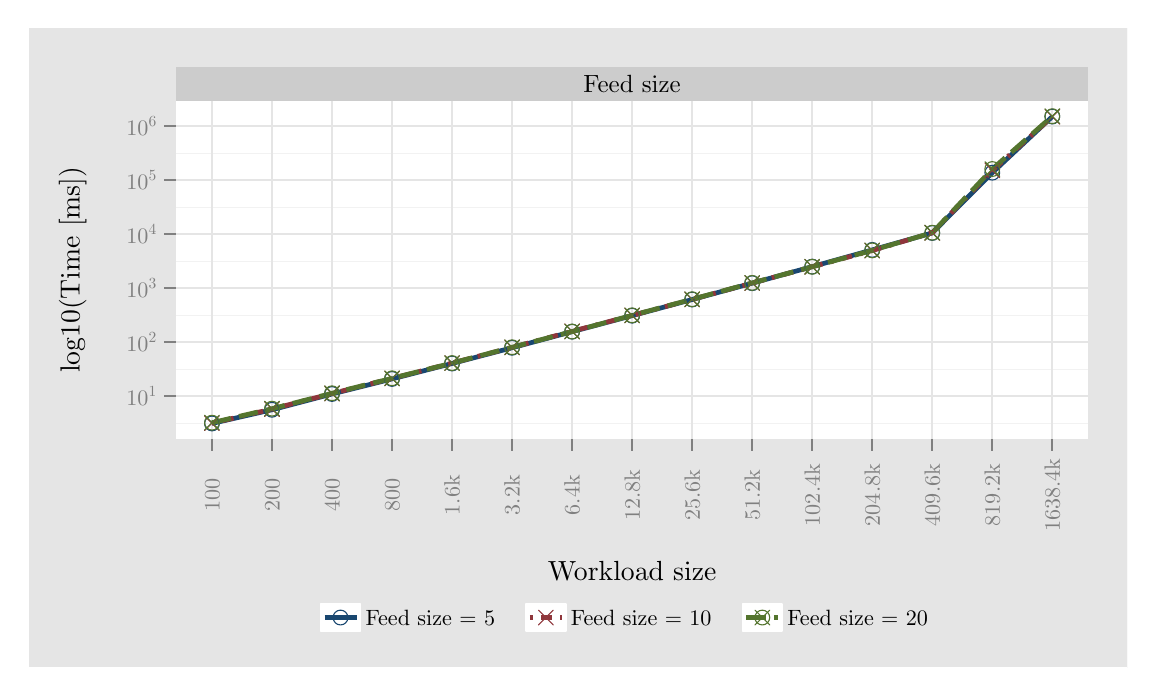
\begin{tikzpicture}[x=1pt,y=1pt]
\definecolor[named]{fillColor}{rgb}{1.00,1.00,1.00}
\path[use as bounding box,fill=fillColor,fill opacity=0.00] (0,0) rectangle (397.48,231.26);
\begin{scope}
\path[clip] (  0.00,  0.00) rectangle (397.48,231.26);
\definecolor[named]{drawColor}{rgb}{1.00,1.00,1.00}
\definecolor[named]{fillColor}{rgb}{0.90,0.90,0.90}

\path[draw=drawColor,line width= 0.6pt,line join=round,line cap=round,fill=fillColor] (  0.00,  0.00) rectangle (397.48,231.26);
\end{scope}
\begin{scope}
\path[clip] ( 53.58, 82.69) rectangle (383.26,204.82);
\definecolor[named]{fillColor}{rgb}{1.00,1.00,1.00}

\path[fill=fillColor] ( 53.58, 82.69) rectangle (383.26,204.82);
\definecolor[named]{drawColor}{rgb}{0.95,0.95,0.95}

\path[draw=drawColor,line width= 0.3pt,line join=round] ( 53.58, 88.33) --
	(383.26, 88.33);

\path[draw=drawColor,line width= 0.3pt,line join=round] ( 53.58,107.85) --
	(383.26,107.85);

\path[draw=drawColor,line width= 0.3pt,line join=round] ( 53.58,127.36) --
	(383.26,127.36);

\path[draw=drawColor,line width= 0.3pt,line join=round] ( 53.58,146.88) --
	(383.26,146.88);

\path[draw=drawColor,line width= 0.3pt,line join=round] ( 53.58,166.40) --
	(383.26,166.40);

\path[draw=drawColor,line width= 0.3pt,line join=round] ( 53.58,185.92) --
	(383.26,185.92);
\definecolor[named]{drawColor}{rgb}{0.90,0.90,0.90}

\path[draw=drawColor,line width= 0.6pt,line join=round] ( 53.58, 98.09) --
	(383.26, 98.09);

\path[draw=drawColor,line width= 0.6pt,line join=round] ( 53.58,117.60) --
	(383.26,117.60);

\path[draw=drawColor,line width= 0.6pt,line join=round] ( 53.58,137.12) --
	(383.26,137.12);

\path[draw=drawColor,line width= 0.6pt,line join=round] ( 53.58,156.64) --
	(383.26,156.64);

\path[draw=drawColor,line width= 0.6pt,line join=round] ( 53.58,176.16) --
	(383.26,176.16);

\path[draw=drawColor,line width= 0.6pt,line join=round] ( 53.58,195.68) --
	(383.26,195.68);

\path[draw=drawColor,line width= 0.6pt,line join=round] ( 66.60, 82.69) --
	( 66.60,204.82);

\path[draw=drawColor,line width= 0.6pt,line join=round] ( 88.29, 82.69) --
	( 88.29,204.82);

\path[draw=drawColor,line width= 0.6pt,line join=round] (109.97, 82.69) --
	(109.97,204.82);

\path[draw=drawColor,line width= 0.6pt,line join=round] (131.66, 82.69) --
	(131.66,204.82);

\path[draw=drawColor,line width= 0.6pt,line join=round] (153.35, 82.69) --
	(153.35,204.82);

\path[draw=drawColor,line width= 0.6pt,line join=round] (175.04, 82.69) --
	(175.04,204.82);

\path[draw=drawColor,line width= 0.6pt,line join=round] (196.73, 82.69) --
	(196.73,204.82);

\path[draw=drawColor,line width= 0.6pt,line join=round] (218.42, 82.69) --
	(218.42,204.82);

\path[draw=drawColor,line width= 0.6pt,line join=round] (240.11, 82.69) --
	(240.11,204.82);

\path[draw=drawColor,line width= 0.6pt,line join=round] (261.80, 82.69) --
	(261.80,204.82);

\path[draw=drawColor,line width= 0.6pt,line join=round] (283.49, 82.69) --
	(283.49,204.82);

\path[draw=drawColor,line width= 0.6pt,line join=round] (305.18, 82.69) --
	(305.18,204.82);

\path[draw=drawColor,line width= 0.6pt,line join=round] (326.87, 82.69) --
	(326.87,204.82);

\path[draw=drawColor,line width= 0.6pt,line join=round] (348.56, 82.69) --
	(348.56,204.82);

\path[draw=drawColor,line width= 0.6pt,line join=round] (370.25, 82.69) --
	(370.25,204.82);
\definecolor[named]{drawColor}{rgb}{0.10,0.28,0.44}

\path[draw=drawColor,line width= 1.7pt,line join=round] ( 66.60, 88.24) --
	( 88.29, 93.19) --
	(109.97, 98.89) --
	(131.66,104.33) --
	(153.35,109.91) --
	(175.04,115.59) --
	(196.73,121.41) --
	(218.42,127.19) --
	(240.11,133.03) --
	(261.80,138.93) --
	(283.49,144.91) --
	(305.18,150.96) --
	(326.87,157.08) --
	(348.56,178.86) --
	(370.25,199.14);
\definecolor[named]{drawColor}{rgb}{0.56,0.21,0.23}

\path[draw=drawColor,line width= 1.7pt,dash pattern=on 1pt off 3pt on 4pt off 3pt ,line join=round] ( 66.60, 88.33) --
	( 88.29, 93.46) --
	(109.97, 99.06) --
	(131.66,104.52) --
	(153.35,110.08) --
	(175.04,115.73) --
	(196.73,121.56) --
	(218.42,127.27) --
	(240.11,133.06) --
	(261.80,138.96) --
	(283.49,144.85) --
	(305.18,150.70) --
	(326.87,157.16) --
	(348.56,179.65) --
	(370.25,199.08);
\definecolor[named]{drawColor}{rgb}{0.33,0.46,0.18}

\path[draw=drawColor,line width= 1.7pt,dash pattern=on 7pt off 3pt ,line join=round] ( 66.60, 88.52) --
	( 88.29, 93.58) --
	(109.97, 99.15) --
	(131.66,104.56) --
	(153.35,110.06) --
	(175.04,115.78) --
	(196.73,121.45) --
	(218.42,127.31) --
	(240.11,133.13) --
	(261.80,139.03) --
	(283.49,144.86) --
	(305.18,150.78) --
	(326.87,157.16) --
	(348.56,180.18) --
	(370.25,199.27);
\definecolor[named]{drawColor}{rgb}{0.10,0.28,0.44}

\path[draw=drawColor,line width= 0.4pt,line join=round,line cap=round] ( 66.60, 88.24) circle (  2.67);

\path[draw=drawColor,line width= 0.4pt,line join=round,line cap=round] ( 88.29, 93.19) circle (  2.67);

\path[draw=drawColor,line width= 0.4pt,line join=round,line cap=round] (109.97, 98.89) circle (  2.67);

\path[draw=drawColor,line width= 0.4pt,line join=round,line cap=round] (131.66,104.33) circle (  2.67);

\path[draw=drawColor,line width= 0.4pt,line join=round,line cap=round] (153.35,109.91) circle (  2.67);

\path[draw=drawColor,line width= 0.4pt,line join=round,line cap=round] (175.04,115.59) circle (  2.67);

\path[draw=drawColor,line width= 0.4pt,line join=round,line cap=round] (196.73,121.41) circle (  2.67);

\path[draw=drawColor,line width= 0.4pt,line join=round,line cap=round] (218.42,127.19) circle (  2.67);

\path[draw=drawColor,line width= 0.4pt,line join=round,line cap=round] (240.11,133.03) circle (  2.67);

\path[draw=drawColor,line width= 0.4pt,line join=round,line cap=round] (261.80,138.93) circle (  2.67);

\path[draw=drawColor,line width= 0.4pt,line join=round,line cap=round] (283.49,144.91) circle (  2.67);

\path[draw=drawColor,line width= 0.4pt,line join=round,line cap=round] (305.18,150.96) circle (  2.67);

\path[draw=drawColor,line width= 0.4pt,line join=round,line cap=round] (326.87,157.08) circle (  2.67);

\path[draw=drawColor,line width= 0.4pt,line join=round,line cap=round] (348.56,178.86) circle (  2.67);

\path[draw=drawColor,line width= 0.4pt,line join=round,line cap=round] (370.25,199.14) circle (  2.67);
\definecolor[named]{drawColor}{rgb}{0.56,0.21,0.23}

\path[draw=drawColor,line width= 0.4pt,line join=round,line cap=round,fill=fillColor] ( 63.93, 85.66) -- ( 69.26, 91.00);

\path[draw=drawColor,line width= 0.4pt,line join=round,line cap=round,fill=fillColor] ( 63.93, 91.00) -- ( 69.26, 85.66);

\path[draw=drawColor,line width= 0.4pt,line join=round,line cap=round,fill=fillColor] ( 85.62, 90.80) -- ( 90.95, 96.13);

\path[draw=drawColor,line width= 0.4pt,line join=round,line cap=round,fill=fillColor] ( 85.62, 96.13) -- ( 90.95, 90.80);

\path[draw=drawColor,line width= 0.4pt,line join=round,line cap=round,fill=fillColor] (107.31, 96.40) -- (112.64,101.73);

\path[draw=drawColor,line width= 0.4pt,line join=round,line cap=round,fill=fillColor] (107.31,101.73) -- (112.64, 96.40);

\path[draw=drawColor,line width= 0.4pt,line join=round,line cap=round,fill=fillColor] (129.00,101.85) -- (134.33,107.18);

\path[draw=drawColor,line width= 0.4pt,line join=round,line cap=round,fill=fillColor] (129.00,107.18) -- (134.33,101.85);

\path[draw=drawColor,line width= 0.4pt,line join=round,line cap=round,fill=fillColor] (150.69,107.41) -- (156.02,112.74);

\path[draw=drawColor,line width= 0.4pt,line join=round,line cap=round,fill=fillColor] (150.69,112.74) -- (156.02,107.41);

\path[draw=drawColor,line width= 0.4pt,line join=round,line cap=round,fill=fillColor] (172.37,113.06) -- (177.71,118.40);

\path[draw=drawColor,line width= 0.4pt,line join=round,line cap=round,fill=fillColor] (172.37,118.40) -- (177.71,113.06);

\path[draw=drawColor,line width= 0.4pt,line join=round,line cap=round,fill=fillColor] (194.06,118.90) -- (199.40,124.23);

\path[draw=drawColor,line width= 0.4pt,line join=round,line cap=round,fill=fillColor] (194.06,124.23) -- (199.40,118.90);

\path[draw=drawColor,line width= 0.4pt,line join=round,line cap=round,fill=fillColor] (215.75,124.61) -- (221.09,129.94);

\path[draw=drawColor,line width= 0.4pt,line join=round,line cap=round,fill=fillColor] (215.75,129.94) -- (221.09,124.61);

\path[draw=drawColor,line width= 0.4pt,line join=round,line cap=round,fill=fillColor] (237.44,130.39) -- (242.78,135.73);

\path[draw=drawColor,line width= 0.4pt,line join=round,line cap=round,fill=fillColor] (237.44,135.73) -- (242.78,130.39);

\path[draw=drawColor,line width= 0.4pt,line join=round,line cap=round,fill=fillColor] (259.13,136.29) -- (264.47,141.63);

\path[draw=drawColor,line width= 0.4pt,line join=round,line cap=round,fill=fillColor] (259.13,141.63) -- (264.47,136.29);

\path[draw=drawColor,line width= 0.4pt,line join=round,line cap=round,fill=fillColor] (280.82,142.18) -- (286.16,147.52);

\path[draw=drawColor,line width= 0.4pt,line join=round,line cap=round,fill=fillColor] (280.82,147.52) -- (286.16,142.18);

\path[draw=drawColor,line width= 0.4pt,line join=round,line cap=round,fill=fillColor] (302.51,148.04) -- (307.84,153.37);

\path[draw=drawColor,line width= 0.4pt,line join=round,line cap=round,fill=fillColor] (302.51,153.37) -- (307.84,148.04);

\path[draw=drawColor,line width= 0.4pt,line join=round,line cap=round,fill=fillColor] (324.20,154.49) -- (329.53,159.82);

\path[draw=drawColor,line width= 0.4pt,line join=round,line cap=round,fill=fillColor] (324.20,159.82) -- (329.53,154.49);

\path[draw=drawColor,line width= 0.4pt,line join=round,line cap=round,fill=fillColor] (345.89,176.99) -- (351.22,182.32);

\path[draw=drawColor,line width= 0.4pt,line join=round,line cap=round,fill=fillColor] (345.89,182.32) -- (351.22,176.99);

\path[draw=drawColor,line width= 0.4pt,line join=round,line cap=round,fill=fillColor] (367.58,196.41) -- (372.91,201.75);

\path[draw=drawColor,line width= 0.4pt,line join=round,line cap=round,fill=fillColor] (367.58,201.75) -- (372.91,196.41);
\definecolor[named]{drawColor}{rgb}{0.33,0.46,0.18}

\path[draw=drawColor,line width= 0.4pt,line join=round,line cap=round] ( 66.60, 88.52) circle (  2.67);

\path[draw=drawColor,line width= 0.4pt,line join=round,line cap=round] ( 63.93, 85.85) -- ( 69.26, 91.19);

\path[draw=drawColor,line width= 0.4pt,line join=round,line cap=round] ( 63.93, 91.19) -- ( 69.26, 85.85);

\path[draw=drawColor,line width= 0.4pt,line join=round,line cap=round] ( 88.29, 93.58) circle (  2.67);

\path[draw=drawColor,line width= 0.4pt,line join=round,line cap=round] ( 85.62, 90.91) -- ( 90.95, 96.25);

\path[draw=drawColor,line width= 0.4pt,line join=round,line cap=round] ( 85.62, 96.25) -- ( 90.95, 90.91);

\path[draw=drawColor,line width= 0.4pt,line join=round,line cap=round] (109.97, 99.15) circle (  2.67);

\path[draw=drawColor,line width= 0.4pt,line join=round,line cap=round] (107.31, 96.48) -- (112.64,101.82);

\path[draw=drawColor,line width= 0.4pt,line join=round,line cap=round] (107.31,101.82) -- (112.64, 96.48);

\path[draw=drawColor,line width= 0.4pt,line join=round,line cap=round] (131.66,104.56) circle (  2.67);

\path[draw=drawColor,line width= 0.4pt,line join=round,line cap=round] (129.00,101.89) -- (134.33,107.22);

\path[draw=drawColor,line width= 0.4pt,line join=round,line cap=round] (129.00,107.22) -- (134.33,101.89);

\path[draw=drawColor,line width= 0.4pt,line join=round,line cap=round] (153.35,110.06) circle (  2.67);

\path[draw=drawColor,line width= 0.4pt,line join=round,line cap=round] (150.69,107.40) -- (156.02,112.73);

\path[draw=drawColor,line width= 0.4pt,line join=round,line cap=round] (150.69,112.73) -- (156.02,107.40);

\path[draw=drawColor,line width= 0.4pt,line join=round,line cap=round] (175.04,115.78) circle (  2.67);

\path[draw=drawColor,line width= 0.4pt,line join=round,line cap=round] (172.37,113.12) -- (177.71,118.45);

\path[draw=drawColor,line width= 0.4pt,line join=round,line cap=round] (172.37,118.45) -- (177.71,113.12);

\path[draw=drawColor,line width= 0.4pt,line join=round,line cap=round] (196.73,121.45) circle (  2.67);

\path[draw=drawColor,line width= 0.4pt,line join=round,line cap=round] (194.06,118.78) -- (199.40,124.12);

\path[draw=drawColor,line width= 0.4pt,line join=round,line cap=round] (194.06,124.12) -- (199.40,118.78);

\path[draw=drawColor,line width= 0.4pt,line join=round,line cap=round] (218.42,127.31) circle (  2.67);

\path[draw=drawColor,line width= 0.4pt,line join=round,line cap=round] (215.75,124.65) -- (221.09,129.98);

\path[draw=drawColor,line width= 0.4pt,line join=round,line cap=round] (215.75,129.98) -- (221.09,124.65);

\path[draw=drawColor,line width= 0.4pt,line join=round,line cap=round] (240.11,133.13) circle (  2.67);

\path[draw=drawColor,line width= 0.4pt,line join=round,line cap=round] (237.44,130.46) -- (242.78,135.79);

\path[draw=drawColor,line width= 0.4pt,line join=round,line cap=round] (237.44,135.79) -- (242.78,130.46);

\path[draw=drawColor,line width= 0.4pt,line join=round,line cap=round] (261.80,139.03) circle (  2.67);

\path[draw=drawColor,line width= 0.4pt,line join=round,line cap=round] (259.13,136.37) -- (264.47,141.70);

\path[draw=drawColor,line width= 0.4pt,line join=round,line cap=round] (259.13,141.70) -- (264.47,136.37);

\path[draw=drawColor,line width= 0.4pt,line join=round,line cap=round] (283.49,144.86) circle (  2.67);

\path[draw=drawColor,line width= 0.4pt,line join=round,line cap=round] (280.82,142.19) -- (286.16,147.53);

\path[draw=drawColor,line width= 0.4pt,line join=round,line cap=round] (280.82,147.53) -- (286.16,142.19);

\path[draw=drawColor,line width= 0.4pt,line join=round,line cap=round] (305.18,150.78) circle (  2.67);

\path[draw=drawColor,line width= 0.4pt,line join=round,line cap=round] (302.51,148.11) -- (307.84,153.45);

\path[draw=drawColor,line width= 0.4pt,line join=round,line cap=round] (302.51,153.45) -- (307.84,148.11);

\path[draw=drawColor,line width= 0.4pt,line join=round,line cap=round] (326.87,157.16) circle (  2.67);

\path[draw=drawColor,line width= 0.4pt,line join=round,line cap=round] (324.20,154.49) -- (329.53,159.82);

\path[draw=drawColor,line width= 0.4pt,line join=round,line cap=round] (324.20,159.82) -- (329.53,154.49);

\path[draw=drawColor,line width= 0.4pt,line join=round,line cap=round] (348.56,180.18) circle (  2.67);

\path[draw=drawColor,line width= 0.4pt,line join=round,line cap=round] (345.89,177.51) -- (351.22,182.84);

\path[draw=drawColor,line width= 0.4pt,line join=round,line cap=round] (345.89,182.84) -- (351.22,177.51);

\path[draw=drawColor,line width= 0.4pt,line join=round,line cap=round] (370.25,199.27) circle (  2.67);

\path[draw=drawColor,line width= 0.4pt,line join=round,line cap=round] (367.58,196.60) -- (372.91,201.93);

\path[draw=drawColor,line width= 0.4pt,line join=round,line cap=round] (367.58,201.93) -- (372.91,196.60);
\end{scope}
\begin{scope}
\path[clip] (  0.00,  0.00) rectangle (397.48,231.26);
\definecolor[named]{fillColor}{rgb}{0.80,0.80,0.80}

\path[fill=fillColor] ( 53.58,204.82) rectangle (383.26,217.04);
\definecolor[named]{drawColor}{rgb}{0.00,0.00,0.00}

\node[text=drawColor,anchor=base,inner sep=0pt, outer sep=0pt, scale=  0.90] at (218.42,207.83) {Feed size};
\end{scope}
\begin{scope}
\path[clip] (  0.00,  0.00) rectangle (397.48,231.26);
\definecolor[named]{drawColor}{rgb}{0.50,0.50,0.50}

\node[text=drawColor,anchor=base west,inner sep=0pt, outer sep=0pt, scale=  0.80] at ( 35.67, 94.65) {10};

\node[text=drawColor,anchor=base west,inner sep=0pt, outer sep=0pt, scale=  0.56] at ( 43.67, 97.93) {1};

\node[text=drawColor,anchor=base west,inner sep=0pt, outer sep=0pt, scale=  0.80] at ( 35.67,114.17) {10};

\node[text=drawColor,anchor=base west,inner sep=0pt, outer sep=0pt, scale=  0.56] at ( 43.67,117.44) {2};

\node[text=drawColor,anchor=base west,inner sep=0pt, outer sep=0pt, scale=  0.80] at ( 35.67,133.69) {10};

\node[text=drawColor,anchor=base west,inner sep=0pt, outer sep=0pt, scale=  0.56] at ( 43.67,136.96) {3};

\node[text=drawColor,anchor=base west,inner sep=0pt, outer sep=0pt, scale=  0.80] at ( 35.67,153.21) {10};

\node[text=drawColor,anchor=base west,inner sep=0pt, outer sep=0pt, scale=  0.56] at ( 43.67,156.48) {4};

\node[text=drawColor,anchor=base west,inner sep=0pt, outer sep=0pt, scale=  0.80] at ( 35.67,172.73) {10};

\node[text=drawColor,anchor=base west,inner sep=0pt, outer sep=0pt, scale=  0.56] at ( 43.67,176.00) {5};

\node[text=drawColor,anchor=base west,inner sep=0pt, outer sep=0pt, scale=  0.80] at ( 35.67,192.25) {10};

\node[text=drawColor,anchor=base west,inner sep=0pt, outer sep=0pt, scale=  0.56] at ( 43.67,195.52) {6};
\end{scope}
\begin{scope}
\path[clip] (  0.00,  0.00) rectangle (397.48,231.26);
\definecolor[named]{drawColor}{rgb}{0.50,0.50,0.50}

\path[draw=drawColor,line width= 0.6pt,line join=round] ( 49.31, 98.09) --
	( 53.58, 98.09);

\path[draw=drawColor,line width= 0.6pt,line join=round] ( 49.31,117.60) --
	( 53.58,117.60);

\path[draw=drawColor,line width= 0.6pt,line join=round] ( 49.31,137.12) --
	( 53.58,137.12);

\path[draw=drawColor,line width= 0.6pt,line join=round] ( 49.31,156.64) --
	( 53.58,156.64);

\path[draw=drawColor,line width= 0.6pt,line join=round] ( 49.31,176.16) --
	( 53.58,176.16);

\path[draw=drawColor,line width= 0.6pt,line join=round] ( 49.31,195.68) --
	( 53.58,195.68);
\end{scope}
\begin{scope}
\path[clip] (  0.00,  0.00) rectangle (397.48,231.26);
\definecolor[named]{drawColor}{rgb}{0.50,0.50,0.50}

\path[draw=drawColor,line width= 0.6pt,line join=round] ( 66.60, 78.42) --
	( 66.60, 82.69);

\path[draw=drawColor,line width= 0.6pt,line join=round] ( 88.29, 78.42) --
	( 88.29, 82.69);

\path[draw=drawColor,line width= 0.6pt,line join=round] (109.97, 78.42) --
	(109.97, 82.69);

\path[draw=drawColor,line width= 0.6pt,line join=round] (131.66, 78.42) --
	(131.66, 82.69);

\path[draw=drawColor,line width= 0.6pt,line join=round] (153.35, 78.42) --
	(153.35, 82.69);

\path[draw=drawColor,line width= 0.6pt,line join=round] (175.04, 78.42) --
	(175.04, 82.69);

\path[draw=drawColor,line width= 0.6pt,line join=round] (196.73, 78.42) --
	(196.73, 82.69);

\path[draw=drawColor,line width= 0.6pt,line join=round] (218.42, 78.42) --
	(218.42, 82.69);

\path[draw=drawColor,line width= 0.6pt,line join=round] (240.11, 78.42) --
	(240.11, 82.69);

\path[draw=drawColor,line width= 0.6pt,line join=round] (261.80, 78.42) --
	(261.80, 82.69);

\path[draw=drawColor,line width= 0.6pt,line join=round] (283.49, 78.42) --
	(283.49, 82.69);

\path[draw=drawColor,line width= 0.6pt,line join=round] (305.18, 78.42) --
	(305.18, 82.69);

\path[draw=drawColor,line width= 0.6pt,line join=round] (326.87, 78.42) --
	(326.87, 82.69);

\path[draw=drawColor,line width= 0.6pt,line join=round] (348.56, 78.42) --
	(348.56, 82.69);

\path[draw=drawColor,line width= 0.6pt,line join=round] (370.25, 78.42) --
	(370.25, 82.69);
\end{scope}
\begin{scope}
\path[clip] (  0.00,  0.00) rectangle (397.48,231.26);
\definecolor[named]{drawColor}{rgb}{0.50,0.50,0.50}

\node[text=drawColor,rotate= 90.00,anchor=base,inner sep=0pt, outer sep=0pt, scale=  0.80] at ( 69.35, 62.36) {100};

\node[text=drawColor,rotate= 90.00,anchor=base,inner sep=0pt, outer sep=0pt, scale=  0.80] at ( 91.04, 62.36) {200};

\node[text=drawColor,rotate= 90.00,anchor=base,inner sep=0pt, outer sep=0pt, scale=  0.80] at (112.73, 62.36) {400};

\node[text=drawColor,rotate= 90.00,anchor=base,inner sep=0pt, outer sep=0pt, scale=  0.80] at (134.42, 62.36) {800};

\node[text=drawColor,rotate= 90.00,anchor=base,inner sep=0pt, outer sep=0pt, scale=  0.80] at (156.11, 62.36) {1.6k};

\node[text=drawColor,rotate= 90.00,anchor=base,inner sep=0pt, outer sep=0pt, scale=  0.80] at (177.80, 62.36) {3.2k};

\node[text=drawColor,rotate= 90.00,anchor=base,inner sep=0pt, outer sep=0pt, scale=  0.80] at (199.49, 62.36) {6.4k};

\node[text=drawColor,rotate= 90.00,anchor=base,inner sep=0pt, outer sep=0pt, scale=  0.80] at (221.18, 62.36) {12.8k};

\node[text=drawColor,rotate= 90.00,anchor=base,inner sep=0pt, outer sep=0pt, scale=  0.80] at (242.86, 62.36) {25.6k};

\node[text=drawColor,rotate= 90.00,anchor=base,inner sep=0pt, outer sep=0pt, scale=  0.80] at (264.55, 62.36) {51.2k};

\node[text=drawColor,rotate= 90.00,anchor=base,inner sep=0pt, outer sep=0pt, scale=  0.80] at (286.24, 62.36) {102.4k};

\node[text=drawColor,rotate= 90.00,anchor=base,inner sep=0pt, outer sep=0pt, scale=  0.80] at (307.93, 62.36) {204.8k};

\node[text=drawColor,rotate= 90.00,anchor=base,inner sep=0pt, outer sep=0pt, scale=  0.80] at (329.62, 62.36) {409.6k};

\node[text=drawColor,rotate= 90.00,anchor=base,inner sep=0pt, outer sep=0pt, scale=  0.80] at (351.31, 62.36) {819.2k};

\node[text=drawColor,rotate= 90.00,anchor=base,inner sep=0pt, outer sep=0pt, scale=  0.80] at (373.00, 62.36) {1638.4k};
\end{scope}
\begin{scope}
\path[clip] (  0.00,  0.00) rectangle (397.48,231.26);
\definecolor[named]{drawColor}{rgb}{0.00,0.00,0.00}

\node[text=drawColor,anchor=base,inner sep=0pt, outer sep=0pt, scale=  1.00] at (218.42, 31.41) {Workload size};
\end{scope}
\begin{scope}
\path[clip] (  0.00,  0.00) rectangle (397.48,231.26);
\definecolor[named]{drawColor}{rgb}{0.00,0.00,0.00}

\node[text=drawColor,rotate= 90.00,anchor=base,inner sep=0pt, outer sep=0pt, scale=  1.00] at ( 18.80,143.75) {log10(Time [ms])};
\end{scope}
\begin{scope}
\path[clip] (  0.00,  0.00) rectangle (397.48,231.26);
\definecolor[named]{fillColor}{rgb}{0.90,0.90,0.90}

\path[fill=fillColor] ( 97.93,  8.87) rectangle (338.91, 27.36);
\end{scope}
\begin{scope}
\path[clip] (  0.00,  0.00) rectangle (397.48,231.26);
\definecolor[named]{drawColor}{rgb}{1.00,1.00,1.00}
\definecolor[named]{fillColor}{rgb}{1.00,1.00,1.00}

\path[draw=drawColor,line width= 0.6pt,line join=round,line cap=round,fill=fillColor] (105.82, 13.14) rectangle (120.27, 23.09);
\end{scope}
\begin{scope}
\path[clip] (  0.00,  0.00) rectangle (397.48,231.26);
\definecolor[named]{drawColor}{rgb}{0.10,0.28,0.44}

\path[draw=drawColor,line width= 1.7pt,line join=round] (107.26, 18.11) -- (118.82, 18.11);
\end{scope}
\begin{scope}
\path[clip] (  0.00,  0.00) rectangle (397.48,231.26);
\definecolor[named]{drawColor}{rgb}{0.10,0.28,0.44}

\path[draw=drawColor,line width= 0.4pt,line join=round,line cap=round] (113.04, 18.11) circle (  2.67);
\end{scope}
\begin{scope}
\path[clip] (  0.00,  0.00) rectangle (397.48,231.26);
\definecolor[named]{drawColor}{rgb}{1.00,1.00,1.00}
\definecolor[named]{fillColor}{rgb}{1.00,1.00,1.00}

\path[draw=drawColor,line width= 0.6pt,line join=round,line cap=round,fill=fillColor] (180.03, 13.14) rectangle (194.48, 23.09);
\end{scope}
\begin{scope}
\path[clip] (  0.00,  0.00) rectangle (397.48,231.26);
\definecolor[named]{drawColor}{rgb}{0.56,0.21,0.23}

\path[draw=drawColor,line width= 1.7pt,dash pattern=on 1pt off 3pt on 4pt off 3pt ,line join=round] (181.47, 18.11) -- (193.03, 18.11);
\end{scope}
\begin{scope}
\path[clip] (  0.00,  0.00) rectangle (397.48,231.26);
\definecolor[named]{drawColor}{rgb}{0.56,0.21,0.23}
\definecolor[named]{fillColor}{rgb}{1.00,1.00,1.00}

\path[draw=drawColor,line width= 0.4pt,line join=round,line cap=round,fill=fillColor] (184.59, 15.45) -- (189.92, 20.78);

\path[draw=drawColor,line width= 0.4pt,line join=round,line cap=round,fill=fillColor] (184.59, 20.78) -- (189.92, 15.45);
\end{scope}
\begin{scope}
\path[clip] (  0.00,  0.00) rectangle (397.48,231.26);
\definecolor[named]{drawColor}{rgb}{1.00,1.00,1.00}
\definecolor[named]{fillColor}{rgb}{1.00,1.00,1.00}

\path[draw=drawColor,line width= 0.6pt,line join=round,line cap=round,fill=fillColor] (258.24, 13.14) rectangle (272.69, 23.09);
\end{scope}
\begin{scope}
\path[clip] (  0.00,  0.00) rectangle (397.48,231.26);
\definecolor[named]{drawColor}{rgb}{0.33,0.46,0.18}

\path[draw=drawColor,line width= 1.7pt,dash pattern=on 7pt off 3pt ,line join=round] (259.68, 18.11) -- (271.24, 18.11);
\end{scope}
\begin{scope}
\path[clip] (  0.00,  0.00) rectangle (397.48,231.26);
\definecolor[named]{drawColor}{rgb}{0.33,0.46,0.18}

\path[draw=drawColor,line width= 0.4pt,line join=round,line cap=round] (265.46, 18.11) circle (  2.67);

\path[draw=drawColor,line width= 0.4pt,line join=round,line cap=round] (262.80, 15.45) -- (268.13, 20.78);

\path[draw=drawColor,line width= 0.4pt,line join=round,line cap=round] (262.80, 20.78) -- (268.13, 15.45);
\end{scope}
\begin{scope}
\path[clip] (  0.00,  0.00) rectangle (397.48,231.26);
\definecolor[named]{drawColor}{rgb}{0.00,0.00,0.00}

\node[text=drawColor,anchor=base west,inner sep=0pt, outer sep=0pt, scale=  0.80] at (122.08, 15.36) {Feed size = 5 $\;\;\;$};
\end{scope}
\begin{scope}
\path[clip] (  0.00,  0.00) rectangle (397.48,231.26);
\definecolor[named]{drawColor}{rgb}{0.00,0.00,0.00}

\node[text=drawColor,anchor=base west,inner sep=0pt, outer sep=0pt, scale=  0.80] at (196.29, 15.36) {Feed size = 10 $\;\;\;$};
\end{scope}
\begin{scope}
\path[clip] (  0.00,  0.00) rectangle (397.48,231.26);
\definecolor[named]{drawColor}{rgb}{0.00,0.00,0.00}

\node[text=drawColor,anchor=base west,inner sep=0pt, outer sep=0pt, scale=  0.80] at (274.50, 15.36) {Feed size = 20 $\;\;\;$};
\end{scope}
\end{tikzpicture}

 }
\caption[Impact of feed size on feed generation]{Impact of feed size on feed generation performance}
 \label{fig:experimentation:performance:rss-feed:feed-size}
\end{figure}


\begin{figure}
 \centering
 \framebox[\textwidth]{%
% Created by tikzDevice version 0.6.2-92-0ad2792 on 2013-04-07 18:08:56
% !TEX encoding = UTF-8 Unicode
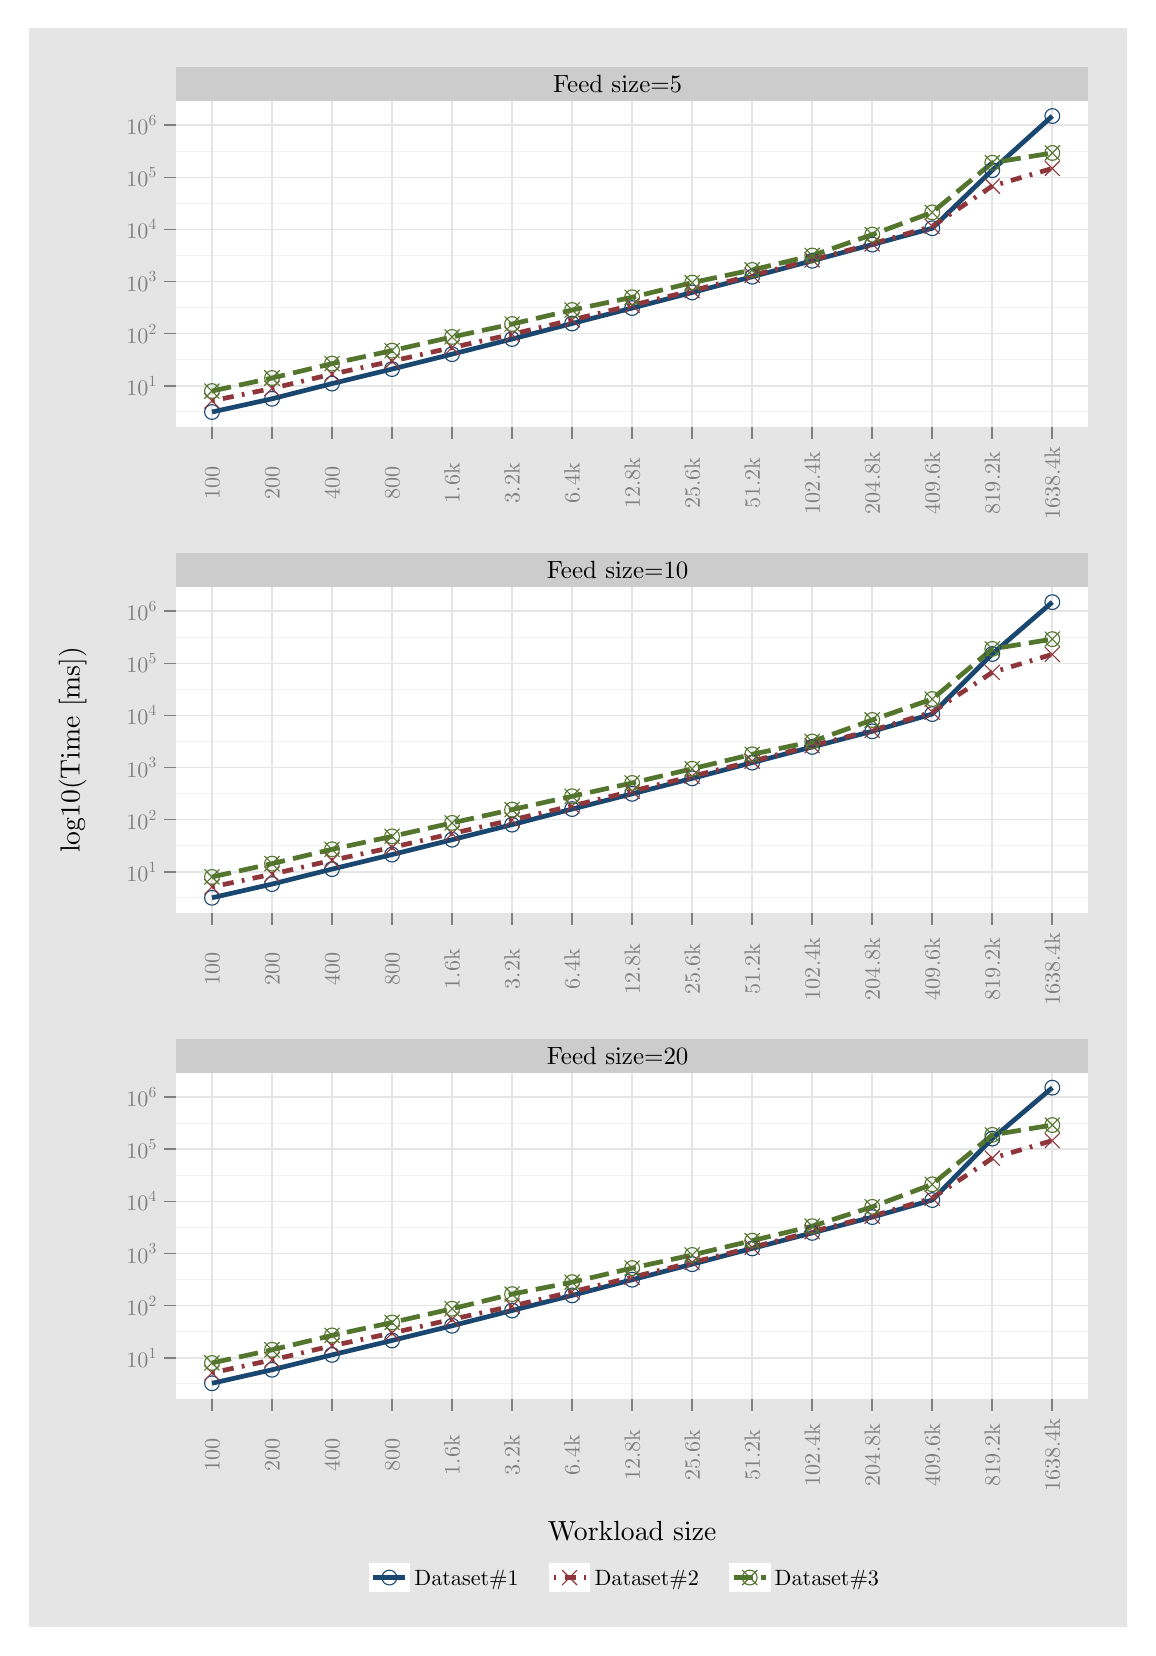
\begin{tikzpicture}[x=1pt,y=1pt]
\definecolor[named]{fillColor}{rgb}{1.00,1.00,1.00}
\path[use as bounding box,fill=fillColor,fill opacity=0.00] (0,0) rectangle (397.48,578.16);
\begin{scope}
\path[clip] (  0.00,  0.00) rectangle (397.48,578.16);
\definecolor[named]{drawColor}{rgb}{1.00,1.00,1.00}
\definecolor[named]{fillColor}{rgb}{0.90,0.90,0.90}

\path[draw=drawColor,line width= 0.6pt,line join=round,line cap=round,fill=fillColor] (  0.00,  0.00) rectangle (397.48,578.16);
\end{scope}
\begin{scope}
\path[clip] ( 53.58,433.92) rectangle (383.26,551.71);
\definecolor[named]{fillColor}{rgb}{1.00,1.00,1.00}

\path[fill=fillColor] ( 53.58,433.92) rectangle (383.26,551.71);
\definecolor[named]{drawColor}{rgb}{0.95,0.95,0.95}

\path[draw=drawColor,line width= 0.3pt,line join=round] ( 53.58,439.35) --
	(383.26,439.35);

\path[draw=drawColor,line width= 0.3pt,line join=round] ( 53.58,458.18) --
	(383.26,458.18);

\path[draw=drawColor,line width= 0.3pt,line join=round] ( 53.58,477.01) --
	(383.26,477.01);

\path[draw=drawColor,line width= 0.3pt,line join=round] ( 53.58,495.83) --
	(383.26,495.83);

\path[draw=drawColor,line width= 0.3pt,line join=round] ( 53.58,514.66) --
	(383.26,514.66);

\path[draw=drawColor,line width= 0.3pt,line join=round] ( 53.58,533.48) --
	(383.26,533.48);
\definecolor[named]{drawColor}{rgb}{0.90,0.90,0.90}

\path[draw=drawColor,line width= 0.6pt,line join=round] ( 53.58,448.77) --
	(383.26,448.77);

\path[draw=drawColor,line width= 0.6pt,line join=round] ( 53.58,467.59) --
	(383.26,467.59);

\path[draw=drawColor,line width= 0.6pt,line join=round] ( 53.58,486.42) --
	(383.26,486.42);

\path[draw=drawColor,line width= 0.6pt,line join=round] ( 53.58,505.25) --
	(383.26,505.25);

\path[draw=drawColor,line width= 0.6pt,line join=round] ( 53.58,524.07) --
	(383.26,524.07);

\path[draw=drawColor,line width= 0.6pt,line join=round] ( 53.58,542.90) --
	(383.26,542.90);

\path[draw=drawColor,line width= 0.6pt,line join=round] ( 66.60,433.92) --
	( 66.60,551.71);

\path[draw=drawColor,line width= 0.6pt,line join=round] ( 88.29,433.92) --
	( 88.29,551.71);

\path[draw=drawColor,line width= 0.6pt,line join=round] (109.97,433.92) --
	(109.97,551.71);

\path[draw=drawColor,line width= 0.6pt,line join=round] (131.66,433.92) --
	(131.66,551.71);

\path[draw=drawColor,line width= 0.6pt,line join=round] (153.35,433.92) --
	(153.35,551.71);

\path[draw=drawColor,line width= 0.6pt,line join=round] (175.04,433.92) --
	(175.04,551.71);

\path[draw=drawColor,line width= 0.6pt,line join=round] (196.73,433.92) --
	(196.73,551.71);

\path[draw=drawColor,line width= 0.6pt,line join=round] (218.42,433.92) --
	(218.42,551.71);

\path[draw=drawColor,line width= 0.6pt,line join=round] (240.11,433.92) --
	(240.11,551.71);

\path[draw=drawColor,line width= 0.6pt,line join=round] (261.80,433.92) --
	(261.80,551.71);

\path[draw=drawColor,line width= 0.6pt,line join=round] (283.49,433.92) --
	(283.49,551.71);

\path[draw=drawColor,line width= 0.6pt,line join=round] (305.18,433.92) --
	(305.18,551.71);

\path[draw=drawColor,line width= 0.6pt,line join=round] (326.87,433.92) --
	(326.87,551.71);

\path[draw=drawColor,line width= 0.6pt,line join=round] (348.56,433.92) --
	(348.56,551.71);

\path[draw=drawColor,line width= 0.6pt,line join=round] (370.25,433.92) --
	(370.25,551.71);
\definecolor[named]{drawColor}{rgb}{0.10,0.28,0.44}

\path[draw=drawColor,line width= 1.7pt,line join=round] ( 66.60,439.27) --
	( 88.29,444.05) --
	(109.97,449.54) --
	(131.66,454.79) --
	(153.35,460.17) --
	(175.04,465.65) --
	(196.73,471.26) --
	(218.42,476.84) --
	(240.11,482.47) --
	(261.80,488.16) --
	(283.49,493.93) --
	(305.18,499.77) --
	(326.87,505.67) --
	(348.56,526.67) --
	(370.25,546.23);
\definecolor[named]{drawColor}{rgb}{0.56,0.21,0.23}

\path[draw=drawColor,line width= 1.7pt,dash pattern=on 1pt off 3pt on 4pt off 3pt ,line join=round] ( 66.60,443.31) --
	( 88.29,447.79) --
	(109.97,452.96) --
	(131.66,457.64) --
	(153.35,462.56) --
	(175.04,467.38) --
	(196.73,472.56) --
	(218.42,477.88) --
	(240.11,483.11) --
	(261.80,488.66) --
	(283.49,494.26) --
	(305.18,500.06) --
	(326.87,506.38) --
	(348.56,520.93) --
	(370.25,527.29);
\definecolor[named]{drawColor}{rgb}{0.33,0.46,0.18}

\path[draw=drawColor,line width= 1.7pt,dash pattern=on 7pt off 3pt ,line join=round] ( 66.60,446.85) --
	( 88.29,451.56) --
	(109.97,456.76) --
	(131.66,461.45) --
	(153.35,466.39) --
	(175.04,471.06) --
	(196.73,476.13) --
	(218.42,480.73) --
	(240.11,486.03) --
	(261.80,490.61) --
	(283.49,495.82) --
	(305.18,503.38) --
	(326.87,511.41) --
	(348.56,529.36) --
	(370.25,532.88);
\definecolor[named]{drawColor}{rgb}{0.10,0.28,0.44}

\path[draw=drawColor,line width= 0.4pt,line join=round,line cap=round] ( 66.60,439.27) circle (  2.67);

\path[draw=drawColor,line width= 0.4pt,line join=round,line cap=round] ( 88.29,444.05) circle (  2.67);

\path[draw=drawColor,line width= 0.4pt,line join=round,line cap=round] (109.97,449.54) circle (  2.67);

\path[draw=drawColor,line width= 0.4pt,line join=round,line cap=round] (131.66,454.79) circle (  2.67);

\path[draw=drawColor,line width= 0.4pt,line join=round,line cap=round] (153.35,460.17) circle (  2.67);

\path[draw=drawColor,line width= 0.4pt,line join=round,line cap=round] (175.04,465.65) circle (  2.67);

\path[draw=drawColor,line width= 0.4pt,line join=round,line cap=round] (196.73,471.26) circle (  2.67);

\path[draw=drawColor,line width= 0.4pt,line join=round,line cap=round] (218.42,476.84) circle (  2.67);

\path[draw=drawColor,line width= 0.4pt,line join=round,line cap=round] (240.11,482.47) circle (  2.67);

\path[draw=drawColor,line width= 0.4pt,line join=round,line cap=round] (261.80,488.16) circle (  2.67);

\path[draw=drawColor,line width= 0.4pt,line join=round,line cap=round] (283.49,493.93) circle (  2.67);

\path[draw=drawColor,line width= 0.4pt,line join=round,line cap=round] (305.18,499.77) circle (  2.67);

\path[draw=drawColor,line width= 0.4pt,line join=round,line cap=round] (326.87,505.67) circle (  2.67);

\path[draw=drawColor,line width= 0.4pt,line join=round,line cap=round] (348.56,526.67) circle (  2.67);

\path[draw=drawColor,line width= 0.4pt,line join=round,line cap=round] (370.25,546.23) circle (  2.67);
\definecolor[named]{drawColor}{rgb}{0.56,0.21,0.23}

\path[draw=drawColor,line width= 0.4pt,line join=round,line cap=round,fill=fillColor] ( 63.93,440.64) -- ( 69.26,445.98);

\path[draw=drawColor,line width= 0.4pt,line join=round,line cap=round,fill=fillColor] ( 63.93,445.98) -- ( 69.26,440.64);

\path[draw=drawColor,line width= 0.4pt,line join=round,line cap=round,fill=fillColor] ( 85.62,445.13) -- ( 90.95,450.46);

\path[draw=drawColor,line width= 0.4pt,line join=round,line cap=round,fill=fillColor] ( 85.62,450.46) -- ( 90.95,445.13);

\path[draw=drawColor,line width= 0.4pt,line join=round,line cap=round,fill=fillColor] (107.31,450.29) -- (112.64,455.63);

\path[draw=drawColor,line width= 0.4pt,line join=round,line cap=round,fill=fillColor] (107.31,455.63) -- (112.64,450.29);

\path[draw=drawColor,line width= 0.4pt,line join=round,line cap=round,fill=fillColor] (129.00,454.97) -- (134.33,460.31);

\path[draw=drawColor,line width= 0.4pt,line join=round,line cap=round,fill=fillColor] (129.00,460.31) -- (134.33,454.97);

\path[draw=drawColor,line width= 0.4pt,line join=round,line cap=round,fill=fillColor] (150.69,459.89) -- (156.02,465.23);

\path[draw=drawColor,line width= 0.4pt,line join=round,line cap=round,fill=fillColor] (150.69,465.23) -- (156.02,459.89);

\path[draw=drawColor,line width= 0.4pt,line join=round,line cap=round,fill=fillColor] (172.37,464.71) -- (177.71,470.04);

\path[draw=drawColor,line width= 0.4pt,line join=round,line cap=round,fill=fillColor] (172.37,470.04) -- (177.71,464.71);

\path[draw=drawColor,line width= 0.4pt,line join=round,line cap=round,fill=fillColor] (194.06,469.90) -- (199.40,475.23);

\path[draw=drawColor,line width= 0.4pt,line join=round,line cap=round,fill=fillColor] (194.06,475.23) -- (199.40,469.90);

\path[draw=drawColor,line width= 0.4pt,line join=round,line cap=round,fill=fillColor] (215.75,475.21) -- (221.09,480.55);

\path[draw=drawColor,line width= 0.4pt,line join=round,line cap=round,fill=fillColor] (215.75,480.55) -- (221.09,475.21);

\path[draw=drawColor,line width= 0.4pt,line join=round,line cap=round,fill=fillColor] (237.44,480.44) -- (242.78,485.78);

\path[draw=drawColor,line width= 0.4pt,line join=round,line cap=round,fill=fillColor] (237.44,485.78) -- (242.78,480.44);

\path[draw=drawColor,line width= 0.4pt,line join=round,line cap=round,fill=fillColor] (259.13,485.99) -- (264.47,491.33);

\path[draw=drawColor,line width= 0.4pt,line join=round,line cap=round,fill=fillColor] (259.13,491.33) -- (264.47,485.99);

\path[draw=drawColor,line width= 0.4pt,line join=round,line cap=round,fill=fillColor] (280.82,491.59) -- (286.16,496.93);

\path[draw=drawColor,line width= 0.4pt,line join=round,line cap=round,fill=fillColor] (280.82,496.93) -- (286.16,491.59);

\path[draw=drawColor,line width= 0.4pt,line join=round,line cap=round,fill=fillColor] (302.51,497.40) -- (307.84,502.73);

\path[draw=drawColor,line width= 0.4pt,line join=round,line cap=round,fill=fillColor] (302.51,502.73) -- (307.84,497.40);

\path[draw=drawColor,line width= 0.4pt,line join=round,line cap=round,fill=fillColor] (324.20,503.71) -- (329.53,509.04);

\path[draw=drawColor,line width= 0.4pt,line join=round,line cap=round,fill=fillColor] (324.20,509.04) -- (329.53,503.71);

\path[draw=drawColor,line width= 0.4pt,line join=round,line cap=round,fill=fillColor] (345.89,518.26) -- (351.22,523.60);

\path[draw=drawColor,line width= 0.4pt,line join=round,line cap=round,fill=fillColor] (345.89,523.60) -- (351.22,518.26);

\path[draw=drawColor,line width= 0.4pt,line join=round,line cap=round,fill=fillColor] (367.58,524.63) -- (372.91,529.96);

\path[draw=drawColor,line width= 0.4pt,line join=round,line cap=round,fill=fillColor] (367.58,529.96) -- (372.91,524.63);
\definecolor[named]{drawColor}{rgb}{0.33,0.46,0.18}

\path[draw=drawColor,line width= 0.4pt,line join=round,line cap=round] ( 66.60,446.85) circle (  2.67);

\path[draw=drawColor,line width= 0.4pt,line join=round,line cap=round] ( 63.93,444.18) -- ( 69.26,449.52);

\path[draw=drawColor,line width= 0.4pt,line join=round,line cap=round] ( 63.93,449.52) -- ( 69.26,444.18);

\path[draw=drawColor,line width= 0.4pt,line join=round,line cap=round] ( 88.29,451.56) circle (  2.67);

\path[draw=drawColor,line width= 0.4pt,line join=round,line cap=round] ( 85.62,448.89) -- ( 90.95,454.23);

\path[draw=drawColor,line width= 0.4pt,line join=round,line cap=round] ( 85.62,454.23) -- ( 90.95,448.89);

\path[draw=drawColor,line width= 0.4pt,line join=round,line cap=round] (109.97,456.76) circle (  2.67);

\path[draw=drawColor,line width= 0.4pt,line join=round,line cap=round] (107.31,454.10) -- (112.64,459.43);

\path[draw=drawColor,line width= 0.4pt,line join=round,line cap=round] (107.31,459.43) -- (112.64,454.10);

\path[draw=drawColor,line width= 0.4pt,line join=round,line cap=round] (131.66,461.45) circle (  2.67);

\path[draw=drawColor,line width= 0.4pt,line join=round,line cap=round] (129.00,458.78) -- (134.33,464.12);

\path[draw=drawColor,line width= 0.4pt,line join=round,line cap=round] (129.00,464.12) -- (134.33,458.78);

\path[draw=drawColor,line width= 0.4pt,line join=round,line cap=round] (153.35,466.39) circle (  2.67);

\path[draw=drawColor,line width= 0.4pt,line join=round,line cap=round] (150.69,463.73) -- (156.02,469.06);

\path[draw=drawColor,line width= 0.4pt,line join=round,line cap=round] (150.69,469.06) -- (156.02,463.73);

\path[draw=drawColor,line width= 0.4pt,line join=round,line cap=round] (175.04,471.06) circle (  2.67);

\path[draw=drawColor,line width= 0.4pt,line join=round,line cap=round] (172.37,468.39) -- (177.71,473.73);

\path[draw=drawColor,line width= 0.4pt,line join=round,line cap=round] (172.37,473.73) -- (177.71,468.39);

\path[draw=drawColor,line width= 0.4pt,line join=round,line cap=round] (196.73,476.13) circle (  2.67);

\path[draw=drawColor,line width= 0.4pt,line join=round,line cap=round] (194.06,473.46) -- (199.40,478.80);

\path[draw=drawColor,line width= 0.4pt,line join=round,line cap=round] (194.06,478.80) -- (199.40,473.46);

\path[draw=drawColor,line width= 0.4pt,line join=round,line cap=round] (218.42,480.73) circle (  2.67);

\path[draw=drawColor,line width= 0.4pt,line join=round,line cap=round] (215.75,478.06) -- (221.09,483.40);

\path[draw=drawColor,line width= 0.4pt,line join=round,line cap=round] (215.75,483.40) -- (221.09,478.06);

\path[draw=drawColor,line width= 0.4pt,line join=round,line cap=round] (240.11,486.03) circle (  2.67);

\path[draw=drawColor,line width= 0.4pt,line join=round,line cap=round] (237.44,483.36) -- (242.78,488.69);

\path[draw=drawColor,line width= 0.4pt,line join=round,line cap=round] (237.44,488.69) -- (242.78,483.36);

\path[draw=drawColor,line width= 0.4pt,line join=round,line cap=round] (261.80,490.61) circle (  2.67);

\path[draw=drawColor,line width= 0.4pt,line join=round,line cap=round] (259.13,487.94) -- (264.47,493.28);

\path[draw=drawColor,line width= 0.4pt,line join=round,line cap=round] (259.13,493.28) -- (264.47,487.94);

\path[draw=drawColor,line width= 0.4pt,line join=round,line cap=round] (283.49,495.82) circle (  2.67);

\path[draw=drawColor,line width= 0.4pt,line join=round,line cap=round] (280.82,493.15) -- (286.16,498.49);

\path[draw=drawColor,line width= 0.4pt,line join=round,line cap=round] (280.82,498.49) -- (286.16,493.15);

\path[draw=drawColor,line width= 0.4pt,line join=round,line cap=round] (305.18,503.38) circle (  2.67);

\path[draw=drawColor,line width= 0.4pt,line join=round,line cap=round] (302.51,500.71) -- (307.84,506.05);

\path[draw=drawColor,line width= 0.4pt,line join=round,line cap=round] (302.51,506.05) -- (307.84,500.71);

\path[draw=drawColor,line width= 0.4pt,line join=round,line cap=round] (326.87,511.41) circle (  2.67);

\path[draw=drawColor,line width= 0.4pt,line join=round,line cap=round] (324.20,508.74) -- (329.53,514.07);

\path[draw=drawColor,line width= 0.4pt,line join=round,line cap=round] (324.20,514.07) -- (329.53,508.74);

\path[draw=drawColor,line width= 0.4pt,line join=round,line cap=round] (348.56,529.36) circle (  2.67);

\path[draw=drawColor,line width= 0.4pt,line join=round,line cap=round] (345.89,526.69) -- (351.22,532.02);

\path[draw=drawColor,line width= 0.4pt,line join=round,line cap=round] (345.89,532.02) -- (351.22,526.69);

\path[draw=drawColor,line width= 0.4pt,line join=round,line cap=round] (370.25,532.88) circle (  2.67);

\path[draw=drawColor,line width= 0.4pt,line join=round,line cap=round] (367.58,530.21) -- (372.91,535.54);

\path[draw=drawColor,line width= 0.4pt,line join=round,line cap=round] (367.58,535.54) -- (372.91,530.21);
\end{scope}
\begin{scope}
\path[clip] ( 53.58,258.30) rectangle (383.26,376.10);
\definecolor[named]{fillColor}{rgb}{1.00,1.00,1.00}

\path[fill=fillColor] ( 53.58,258.30) rectangle (383.26,376.10);
\definecolor[named]{drawColor}{rgb}{0.95,0.95,0.95}

\path[draw=drawColor,line width= 0.3pt,line join=round] ( 53.58,263.74) --
	(383.26,263.74);

\path[draw=drawColor,line width= 0.3pt,line join=round] ( 53.58,282.57) --
	(383.26,282.57);

\path[draw=drawColor,line width= 0.3pt,line join=round] ( 53.58,301.39) --
	(383.26,301.39);

\path[draw=drawColor,line width= 0.3pt,line join=round] ( 53.58,320.22) --
	(383.26,320.22);

\path[draw=drawColor,line width= 0.3pt,line join=round] ( 53.58,339.05) --
	(383.26,339.05);

\path[draw=drawColor,line width= 0.3pt,line join=round] ( 53.58,357.87) --
	(383.26,357.87);
\definecolor[named]{drawColor}{rgb}{0.90,0.90,0.90}

\path[draw=drawColor,line width= 0.6pt,line join=round] ( 53.58,273.15) --
	(383.26,273.15);

\path[draw=drawColor,line width= 0.6pt,line join=round] ( 53.58,291.98) --
	(383.26,291.98);

\path[draw=drawColor,line width= 0.6pt,line join=round] ( 53.58,310.81) --
	(383.26,310.81);

\path[draw=drawColor,line width= 0.6pt,line join=round] ( 53.58,329.63) --
	(383.26,329.63);

\path[draw=drawColor,line width= 0.6pt,line join=round] ( 53.58,348.46) --
	(383.26,348.46);

\path[draw=drawColor,line width= 0.6pt,line join=round] ( 53.58,367.28) --
	(383.26,367.28);

\path[draw=drawColor,line width= 0.6pt,line join=round] ( 66.60,258.30) --
	( 66.60,376.10);

\path[draw=drawColor,line width= 0.6pt,line join=round] ( 88.29,258.30) --
	( 88.29,376.10);

\path[draw=drawColor,line width= 0.6pt,line join=round] (109.97,258.30) --
	(109.97,376.10);

\path[draw=drawColor,line width= 0.6pt,line join=round] (131.66,258.30) --
	(131.66,376.10);

\path[draw=drawColor,line width= 0.6pt,line join=round] (153.35,258.30) --
	(153.35,376.10);

\path[draw=drawColor,line width= 0.6pt,line join=round] (175.04,258.30) --
	(175.04,376.10);

\path[draw=drawColor,line width= 0.6pt,line join=round] (196.73,258.30) --
	(196.73,376.10);

\path[draw=drawColor,line width= 0.6pt,line join=round] (218.42,258.30) --
	(218.42,376.10);

\path[draw=drawColor,line width= 0.6pt,line join=round] (240.11,258.30) --
	(240.11,376.10);

\path[draw=drawColor,line width= 0.6pt,line join=round] (261.80,258.30) --
	(261.80,376.10);

\path[draw=drawColor,line width= 0.6pt,line join=round] (283.49,258.30) --
	(283.49,376.10);

\path[draw=drawColor,line width= 0.6pt,line join=round] (305.18,258.30) --
	(305.18,376.10);

\path[draw=drawColor,line width= 0.6pt,line join=round] (326.87,258.30) --
	(326.87,376.10);

\path[draw=drawColor,line width= 0.6pt,line join=round] (348.56,258.30) --
	(348.56,376.10);

\path[draw=drawColor,line width= 0.6pt,line join=round] (370.25,258.30) --
	(370.25,376.10);
\definecolor[named]{drawColor}{rgb}{0.10,0.28,0.44}

\path[draw=drawColor,line width= 1.7pt,line join=round] ( 66.60,263.74) --
	( 88.29,268.69) --
	(109.97,274.10) --
	(131.66,279.35) --
	(153.35,284.72) --
	(175.04,290.17) --
	(196.73,295.80) --
	(218.42,301.30) --
	(240.11,306.89) --
	(261.80,312.58) --
	(283.49,318.26) --
	(305.18,323.90) --
	(326.87,330.13) --
	(348.56,351.83) --
	(370.25,370.57);
\definecolor[named]{drawColor}{rgb}{0.56,0.21,0.23}

\path[draw=drawColor,line width= 1.7pt,dash pattern=on 1pt off 3pt on 4pt off 3pt ,line join=round] ( 66.60,267.67) --
	( 88.29,272.26) --
	(109.97,277.29) --
	(131.66,281.93) --
	(153.35,286.96) --
	(175.04,291.88) --
	(196.73,296.94) --
	(218.42,302.27) --
	(240.11,307.65) --
	(261.80,313.09) --
	(283.49,318.73) --
	(305.18,324.25) --
	(326.87,330.83) --
	(348.56,345.21) --
	(370.25,351.69);
\definecolor[named]{drawColor}{rgb}{0.33,0.46,0.18}

\path[draw=drawColor,line width= 1.7pt,dash pattern=on 7pt off 3pt ,line join=round] ( 66.60,271.27) --
	( 88.29,276.08) --
	(109.97,281.26) --
	(131.66,285.93) --
	(153.35,290.80) --
	(175.04,295.61) --
	(196.73,300.44) --
	(218.42,305.23) --
	(240.11,310.35) --
	(261.80,315.58) --
	(283.49,320.21) --
	(305.18,327.99) --
	(326.87,335.56) --
	(348.56,353.67) --
	(370.25,357.20);
\definecolor[named]{drawColor}{rgb}{0.10,0.28,0.44}

\path[draw=drawColor,line width= 0.4pt,line join=round,line cap=round] ( 66.60,263.74) circle (  2.67);

\path[draw=drawColor,line width= 0.4pt,line join=round,line cap=round] ( 88.29,268.69) circle (  2.67);

\path[draw=drawColor,line width= 0.4pt,line join=round,line cap=round] (109.97,274.10) circle (  2.67);

\path[draw=drawColor,line width= 0.4pt,line join=round,line cap=round] (131.66,279.35) circle (  2.67);

\path[draw=drawColor,line width= 0.4pt,line join=round,line cap=round] (153.35,284.72) circle (  2.67);

\path[draw=drawColor,line width= 0.4pt,line join=round,line cap=round] (175.04,290.17) circle (  2.67);

\path[draw=drawColor,line width= 0.4pt,line join=round,line cap=round] (196.73,295.80) circle (  2.67);

\path[draw=drawColor,line width= 0.4pt,line join=round,line cap=round] (218.42,301.30) circle (  2.67);

\path[draw=drawColor,line width= 0.4pt,line join=round,line cap=round] (240.11,306.89) circle (  2.67);

\path[draw=drawColor,line width= 0.4pt,line join=round,line cap=round] (261.80,312.58) circle (  2.67);

\path[draw=drawColor,line width= 0.4pt,line join=round,line cap=round] (283.49,318.26) circle (  2.67);

\path[draw=drawColor,line width= 0.4pt,line join=round,line cap=round] (305.18,323.90) circle (  2.67);

\path[draw=drawColor,line width= 0.4pt,line join=round,line cap=round] (326.87,330.13) circle (  2.67);

\path[draw=drawColor,line width= 0.4pt,line join=round,line cap=round] (348.56,351.83) circle (  2.67);

\path[draw=drawColor,line width= 0.4pt,line join=round,line cap=round] (370.25,370.57) circle (  2.67);
\definecolor[named]{drawColor}{rgb}{0.56,0.21,0.23}

\path[draw=drawColor,line width= 0.4pt,line join=round,line cap=round,fill=fillColor] ( 63.93,265.00) -- ( 69.26,270.34);

\path[draw=drawColor,line width= 0.4pt,line join=round,line cap=round,fill=fillColor] ( 63.93,270.34) -- ( 69.26,265.00);

\path[draw=drawColor,line width= 0.4pt,line join=round,line cap=round,fill=fillColor] ( 85.62,269.59) -- ( 90.95,274.93);

\path[draw=drawColor,line width= 0.4pt,line join=round,line cap=round,fill=fillColor] ( 85.62,274.93) -- ( 90.95,269.59);

\path[draw=drawColor,line width= 0.4pt,line join=round,line cap=round,fill=fillColor] (107.31,274.63) -- (112.64,279.96);

\path[draw=drawColor,line width= 0.4pt,line join=round,line cap=round,fill=fillColor] (107.31,279.96) -- (112.64,274.63);

\path[draw=drawColor,line width= 0.4pt,line join=round,line cap=round,fill=fillColor] (129.00,279.27) -- (134.33,284.60);

\path[draw=drawColor,line width= 0.4pt,line join=round,line cap=round,fill=fillColor] (129.00,284.60) -- (134.33,279.27);

\path[draw=drawColor,line width= 0.4pt,line join=round,line cap=round,fill=fillColor] (150.69,284.29) -- (156.02,289.63);

\path[draw=drawColor,line width= 0.4pt,line join=round,line cap=round,fill=fillColor] (150.69,289.63) -- (156.02,284.29);

\path[draw=drawColor,line width= 0.4pt,line join=round,line cap=round,fill=fillColor] (172.37,289.21) -- (177.71,294.55);

\path[draw=drawColor,line width= 0.4pt,line join=round,line cap=round,fill=fillColor] (172.37,294.55) -- (177.71,289.21);

\path[draw=drawColor,line width= 0.4pt,line join=round,line cap=round,fill=fillColor] (194.06,294.27) -- (199.40,299.60);

\path[draw=drawColor,line width= 0.4pt,line join=round,line cap=round,fill=fillColor] (194.06,299.60) -- (199.40,294.27);

\path[draw=drawColor,line width= 0.4pt,line join=round,line cap=round,fill=fillColor] (215.75,299.60) -- (221.09,304.94);

\path[draw=drawColor,line width= 0.4pt,line join=round,line cap=round,fill=fillColor] (215.75,304.94) -- (221.09,299.60);

\path[draw=drawColor,line width= 0.4pt,line join=round,line cap=round,fill=fillColor] (237.44,304.98) -- (242.78,310.32);

\path[draw=drawColor,line width= 0.4pt,line join=round,line cap=round,fill=fillColor] (237.44,310.32) -- (242.78,304.98);

\path[draw=drawColor,line width= 0.4pt,line join=round,line cap=round,fill=fillColor] (259.13,310.42) -- (264.47,315.76);

\path[draw=drawColor,line width= 0.4pt,line join=round,line cap=round,fill=fillColor] (259.13,315.76) -- (264.47,310.42);

\path[draw=drawColor,line width= 0.4pt,line join=round,line cap=round,fill=fillColor] (280.82,316.06) -- (286.16,321.40);

\path[draw=drawColor,line width= 0.4pt,line join=round,line cap=round,fill=fillColor] (280.82,321.40) -- (286.16,316.06);

\path[draw=drawColor,line width= 0.4pt,line join=round,line cap=round,fill=fillColor] (302.51,321.58) -- (307.84,326.91);

\path[draw=drawColor,line width= 0.4pt,line join=round,line cap=round,fill=fillColor] (302.51,326.91) -- (307.84,321.58);

\path[draw=drawColor,line width= 0.4pt,line join=round,line cap=round,fill=fillColor] (324.20,328.16) -- (329.53,333.50);

\path[draw=drawColor,line width= 0.4pt,line join=round,line cap=round,fill=fillColor] (324.20,333.50) -- (329.53,328.16);

\path[draw=drawColor,line width= 0.4pt,line join=round,line cap=round,fill=fillColor] (345.89,342.55) -- (351.22,347.88);

\path[draw=drawColor,line width= 0.4pt,line join=round,line cap=round,fill=fillColor] (345.89,347.88) -- (351.22,342.55);

\path[draw=drawColor,line width= 0.4pt,line join=round,line cap=round,fill=fillColor] (367.58,349.02) -- (372.91,354.36);

\path[draw=drawColor,line width= 0.4pt,line join=round,line cap=round,fill=fillColor] (367.58,354.36) -- (372.91,349.02);
\definecolor[named]{drawColor}{rgb}{0.33,0.46,0.18}

\path[draw=drawColor,line width= 0.4pt,line join=round,line cap=round] ( 66.60,271.27) circle (  2.67);

\path[draw=drawColor,line width= 0.4pt,line join=round,line cap=round] ( 63.93,268.60) -- ( 69.26,273.94);

\path[draw=drawColor,line width= 0.4pt,line join=round,line cap=round] ( 63.93,273.94) -- ( 69.26,268.60);

\path[draw=drawColor,line width= 0.4pt,line join=round,line cap=round] ( 88.29,276.08) circle (  2.67);

\path[draw=drawColor,line width= 0.4pt,line join=round,line cap=round] ( 85.62,273.41) -- ( 90.95,278.75);

\path[draw=drawColor,line width= 0.4pt,line join=round,line cap=round] ( 85.62,278.75) -- ( 90.95,273.41);

\path[draw=drawColor,line width= 0.4pt,line join=round,line cap=round] (109.97,281.26) circle (  2.67);

\path[draw=drawColor,line width= 0.4pt,line join=round,line cap=round] (107.31,278.59) -- (112.64,283.92);

\path[draw=drawColor,line width= 0.4pt,line join=round,line cap=round] (107.31,283.92) -- (112.64,278.59);

\path[draw=drawColor,line width= 0.4pt,line join=round,line cap=round] (131.66,285.93) circle (  2.67);

\path[draw=drawColor,line width= 0.4pt,line join=round,line cap=round] (129.00,283.26) -- (134.33,288.59);

\path[draw=drawColor,line width= 0.4pt,line join=round,line cap=round] (129.00,288.59) -- (134.33,283.26);

\path[draw=drawColor,line width= 0.4pt,line join=round,line cap=round] (153.35,290.80) circle (  2.67);

\path[draw=drawColor,line width= 0.4pt,line join=round,line cap=round] (150.69,288.13) -- (156.02,293.47);

\path[draw=drawColor,line width= 0.4pt,line join=round,line cap=round] (150.69,293.47) -- (156.02,288.13);

\path[draw=drawColor,line width= 0.4pt,line join=round,line cap=round] (175.04,295.61) circle (  2.67);

\path[draw=drawColor,line width= 0.4pt,line join=round,line cap=round] (172.37,292.94) -- (177.71,298.27);

\path[draw=drawColor,line width= 0.4pt,line join=round,line cap=round] (172.37,298.27) -- (177.71,292.94);

\path[draw=drawColor,line width= 0.4pt,line join=round,line cap=round] (196.73,300.44) circle (  2.67);

\path[draw=drawColor,line width= 0.4pt,line join=round,line cap=round] (194.06,297.78) -- (199.40,303.11);

\path[draw=drawColor,line width= 0.4pt,line join=round,line cap=round] (194.06,303.11) -- (199.40,297.78);

\path[draw=drawColor,line width= 0.4pt,line join=round,line cap=round] (218.42,305.23) circle (  2.67);

\path[draw=drawColor,line width= 0.4pt,line join=round,line cap=round] (215.75,302.56) -- (221.09,307.90);

\path[draw=drawColor,line width= 0.4pt,line join=round,line cap=round] (215.75,307.90) -- (221.09,302.56);

\path[draw=drawColor,line width= 0.4pt,line join=round,line cap=round] (240.11,310.35) circle (  2.67);

\path[draw=drawColor,line width= 0.4pt,line join=round,line cap=round] (237.44,307.68) -- (242.78,313.02);

\path[draw=drawColor,line width= 0.4pt,line join=round,line cap=round] (237.44,313.02) -- (242.78,307.68);

\path[draw=drawColor,line width= 0.4pt,line join=round,line cap=round] (261.80,315.58) circle (  2.67);

\path[draw=drawColor,line width= 0.4pt,line join=round,line cap=round] (259.13,312.91) -- (264.47,318.25);

\path[draw=drawColor,line width= 0.4pt,line join=round,line cap=round] (259.13,318.25) -- (264.47,312.91);

\path[draw=drawColor,line width= 0.4pt,line join=round,line cap=round] (283.49,320.21) circle (  2.67);

\path[draw=drawColor,line width= 0.4pt,line join=round,line cap=round] (280.82,317.54) -- (286.16,322.88);

\path[draw=drawColor,line width= 0.4pt,line join=round,line cap=round] (280.82,322.88) -- (286.16,317.54);

\path[draw=drawColor,line width= 0.4pt,line join=round,line cap=round] (305.18,327.99) circle (  2.67);

\path[draw=drawColor,line width= 0.4pt,line join=round,line cap=round] (302.51,325.32) -- (307.84,330.66);

\path[draw=drawColor,line width= 0.4pt,line join=round,line cap=round] (302.51,330.66) -- (307.84,325.32);

\path[draw=drawColor,line width= 0.4pt,line join=round,line cap=round] (326.87,335.56) circle (  2.67);

\path[draw=drawColor,line width= 0.4pt,line join=round,line cap=round] (324.20,332.89) -- (329.53,338.22);

\path[draw=drawColor,line width= 0.4pt,line join=round,line cap=round] (324.20,338.22) -- (329.53,332.89);

\path[draw=drawColor,line width= 0.4pt,line join=round,line cap=round] (348.56,353.67) circle (  2.67);

\path[draw=drawColor,line width= 0.4pt,line join=round,line cap=round] (345.89,351.01) -- (351.22,356.34);

\path[draw=drawColor,line width= 0.4pt,line join=round,line cap=round] (345.89,356.34) -- (351.22,351.01);

\path[draw=drawColor,line width= 0.4pt,line join=round,line cap=round] (370.25,357.20) circle (  2.67);

\path[draw=drawColor,line width= 0.4pt,line join=round,line cap=round] (367.58,354.53) -- (372.91,359.87);

\path[draw=drawColor,line width= 0.4pt,line join=round,line cap=round] (367.58,359.87) -- (372.91,354.53);
\end{scope}
\begin{scope}
\path[clip] ( 53.58, 82.69) rectangle (383.26,200.49);
\definecolor[named]{fillColor}{rgb}{1.00,1.00,1.00}

\path[fill=fillColor] ( 53.58, 82.69) rectangle (383.26,200.49);
\definecolor[named]{drawColor}{rgb}{0.95,0.95,0.95}

\path[draw=drawColor,line width= 0.3pt,line join=round] ( 53.58, 88.13) --
	(383.26, 88.13);

\path[draw=drawColor,line width= 0.3pt,line join=round] ( 53.58,106.95) --
	(383.26,106.95);

\path[draw=drawColor,line width= 0.3pt,line join=round] ( 53.58,125.78) --
	(383.26,125.78);

\path[draw=drawColor,line width= 0.3pt,line join=round] ( 53.58,144.61) --
	(383.26,144.61);

\path[draw=drawColor,line width= 0.3pt,line join=round] ( 53.58,163.43) --
	(383.26,163.43);

\path[draw=drawColor,line width= 0.3pt,line join=round] ( 53.58,182.26) --
	(383.26,182.26);
\definecolor[named]{drawColor}{rgb}{0.90,0.90,0.90}

\path[draw=drawColor,line width= 0.6pt,line join=round] ( 53.58, 97.54) --
	(383.26, 97.54);

\path[draw=drawColor,line width= 0.6pt,line join=round] ( 53.58,116.37) --
	(383.26,116.37);

\path[draw=drawColor,line width= 0.6pt,line join=round] ( 53.58,135.19) --
	(383.26,135.19);

\path[draw=drawColor,line width= 0.6pt,line join=round] ( 53.58,154.02) --
	(383.26,154.02);

\path[draw=drawColor,line width= 0.6pt,line join=round] ( 53.58,172.85) --
	(383.26,172.85);

\path[draw=drawColor,line width= 0.6pt,line join=round] ( 53.58,191.67) --
	(383.26,191.67);

\path[draw=drawColor,line width= 0.6pt,line join=round] ( 66.60, 82.69) --
	( 66.60,200.49);

\path[draw=drawColor,line width= 0.6pt,line join=round] ( 88.29, 82.69) --
	( 88.29,200.49);

\path[draw=drawColor,line width= 0.6pt,line join=round] (109.97, 82.69) --
	(109.97,200.49);

\path[draw=drawColor,line width= 0.6pt,line join=round] (131.66, 82.69) --
	(131.66,200.49);

\path[draw=drawColor,line width= 0.6pt,line join=round] (153.35, 82.69) --
	(153.35,200.49);

\path[draw=drawColor,line width= 0.6pt,line join=round] (175.04, 82.69) --
	(175.04,200.49);

\path[draw=drawColor,line width= 0.6pt,line join=round] (196.73, 82.69) --
	(196.73,200.49);

\path[draw=drawColor,line width= 0.6pt,line join=round] (218.42, 82.69) --
	(218.42,200.49);

\path[draw=drawColor,line width= 0.6pt,line join=round] (240.11, 82.69) --
	(240.11,200.49);

\path[draw=drawColor,line width= 0.6pt,line join=round] (261.80, 82.69) --
	(261.80,200.49);

\path[draw=drawColor,line width= 0.6pt,line join=round] (283.49, 82.69) --
	(283.49,200.49);

\path[draw=drawColor,line width= 0.6pt,line join=round] (305.18, 82.69) --
	(305.18,200.49);

\path[draw=drawColor,line width= 0.6pt,line join=round] (326.87, 82.69) --
	(326.87,200.49);

\path[draw=drawColor,line width= 0.6pt,line join=round] (348.56, 82.69) --
	(348.56,200.49);

\path[draw=drawColor,line width= 0.6pt,line join=round] (370.25, 82.69) --
	(370.25,200.49);
\definecolor[named]{drawColor}{rgb}{0.10,0.28,0.44}

\path[draw=drawColor,line width= 1.7pt,line join=round] ( 66.60, 88.31) --
	( 88.29, 93.19) --
	(109.97, 98.57) --
	(131.66,103.78) --
	(153.35,109.09) --
	(175.04,114.61) --
	(196.73,120.07) --
	(218.42,125.73) --
	(240.11,131.34) --
	(261.80,137.04) --
	(283.49,142.65) --
	(305.18,148.36) --
	(326.87,154.52) --
	(348.56,176.72) --
	(370.25,195.13);
\definecolor[named]{drawColor}{rgb}{0.56,0.21,0.23}

\path[draw=drawColor,line width= 1.7pt,dash pattern=on 1pt off 3pt on 4pt off 3pt ,line join=round] ( 66.60, 92.08) --
	( 88.29, 96.74) --
	(109.97,101.86) --
	(131.66,106.47) --
	(153.35,111.42) --
	(175.04,116.20) --
	(196.73,121.36) --
	(218.42,126.63) --
	(240.11,131.99) --
	(261.80,137.42) --
	(283.49,143.14) --
	(305.18,148.70) --
	(326.87,155.24) --
	(348.56,169.64) --
	(370.25,176.01);
\definecolor[named]{drawColor}{rgb}{0.33,0.46,0.18}

\path[draw=drawColor,line width= 1.7pt,dash pattern=on 7pt off 3pt ,line join=round] ( 66.60, 95.65) --
	( 88.29,100.41) --
	(109.97,105.61) --
	(131.66,110.28) --
	(153.35,115.24) --
	(175.04,120.53) --
	(196.73,124.85) --
	(218.42,129.94) --
	(240.11,134.67) --
	(261.80,139.84) --
	(283.49,145.07) --
	(305.18,152.06) --
	(326.87,160.21) --
	(348.56,178.07) --
	(370.25,181.62);
\definecolor[named]{drawColor}{rgb}{0.10,0.28,0.44}

\path[draw=drawColor,line width= 0.4pt,line join=round,line cap=round] ( 66.60, 88.31) circle (  2.67);

\path[draw=drawColor,line width= 0.4pt,line join=round,line cap=round] ( 88.29, 93.19) circle (  2.67);

\path[draw=drawColor,line width= 0.4pt,line join=round,line cap=round] (109.97, 98.57) circle (  2.67);

\path[draw=drawColor,line width= 0.4pt,line join=round,line cap=round] (131.66,103.78) circle (  2.67);

\path[draw=drawColor,line width= 0.4pt,line join=round,line cap=round] (153.35,109.09) circle (  2.67);

\path[draw=drawColor,line width= 0.4pt,line join=round,line cap=round] (175.04,114.61) circle (  2.67);

\path[draw=drawColor,line width= 0.4pt,line join=round,line cap=round] (196.73,120.07) circle (  2.67);

\path[draw=drawColor,line width= 0.4pt,line join=round,line cap=round] (218.42,125.73) circle (  2.67);

\path[draw=drawColor,line width= 0.4pt,line join=round,line cap=round] (240.11,131.34) circle (  2.67);

\path[draw=drawColor,line width= 0.4pt,line join=round,line cap=round] (261.80,137.04) circle (  2.67);

\path[draw=drawColor,line width= 0.4pt,line join=round,line cap=round] (283.49,142.65) circle (  2.67);

\path[draw=drawColor,line width= 0.4pt,line join=round,line cap=round] (305.18,148.36) circle (  2.67);

\path[draw=drawColor,line width= 0.4pt,line join=round,line cap=round] (326.87,154.52) circle (  2.67);

\path[draw=drawColor,line width= 0.4pt,line join=round,line cap=round] (348.56,176.72) circle (  2.67);

\path[draw=drawColor,line width= 0.4pt,line join=round,line cap=round] (370.25,195.13) circle (  2.67);
\definecolor[named]{drawColor}{rgb}{0.56,0.21,0.23}

\path[draw=drawColor,line width= 0.4pt,line join=round,line cap=round,fill=fillColor] ( 63.93, 89.41) -- ( 69.26, 94.75);

\path[draw=drawColor,line width= 0.4pt,line join=round,line cap=round,fill=fillColor] ( 63.93, 94.75) -- ( 69.26, 89.41);

\path[draw=drawColor,line width= 0.4pt,line join=round,line cap=round,fill=fillColor] ( 85.62, 94.07) -- ( 90.95, 99.41);

\path[draw=drawColor,line width= 0.4pt,line join=round,line cap=round,fill=fillColor] ( 85.62, 99.41) -- ( 90.95, 94.07);

\path[draw=drawColor,line width= 0.4pt,line join=round,line cap=round,fill=fillColor] (107.31, 99.19) -- (112.64,104.52);

\path[draw=drawColor,line width= 0.4pt,line join=round,line cap=round,fill=fillColor] (107.31,104.52) -- (112.64, 99.19);

\path[draw=drawColor,line width= 0.4pt,line join=round,line cap=round,fill=fillColor] (129.00,103.80) -- (134.33,109.14);

\path[draw=drawColor,line width= 0.4pt,line join=round,line cap=round,fill=fillColor] (129.00,109.14) -- (134.33,103.80);

\path[draw=drawColor,line width= 0.4pt,line join=round,line cap=round,fill=fillColor] (150.69,108.76) -- (156.02,114.09);

\path[draw=drawColor,line width= 0.4pt,line join=round,line cap=round,fill=fillColor] (150.69,114.09) -- (156.02,108.76);

\path[draw=drawColor,line width= 0.4pt,line join=round,line cap=round,fill=fillColor] (172.37,113.53) -- (177.71,118.86);

\path[draw=drawColor,line width= 0.4pt,line join=round,line cap=round,fill=fillColor] (172.37,118.86) -- (177.71,113.53);

\path[draw=drawColor,line width= 0.4pt,line join=round,line cap=round,fill=fillColor] (194.06,118.69) -- (199.40,124.03);

\path[draw=drawColor,line width= 0.4pt,line join=round,line cap=round,fill=fillColor] (194.06,124.03) -- (199.40,118.69);

\path[draw=drawColor,line width= 0.4pt,line join=round,line cap=round,fill=fillColor] (215.75,123.96) -- (221.09,129.30);

\path[draw=drawColor,line width= 0.4pt,line join=round,line cap=round,fill=fillColor] (215.75,129.30) -- (221.09,123.96);

\path[draw=drawColor,line width= 0.4pt,line join=round,line cap=round,fill=fillColor] (237.44,129.33) -- (242.78,134.66);

\path[draw=drawColor,line width= 0.4pt,line join=round,line cap=round,fill=fillColor] (237.44,134.66) -- (242.78,129.33);

\path[draw=drawColor,line width= 0.4pt,line join=round,line cap=round,fill=fillColor] (259.13,134.76) -- (264.47,140.09);

\path[draw=drawColor,line width= 0.4pt,line join=round,line cap=round,fill=fillColor] (259.13,140.09) -- (264.47,134.76);

\path[draw=drawColor,line width= 0.4pt,line join=round,line cap=round,fill=fillColor] (280.82,140.47) -- (286.16,145.81);

\path[draw=drawColor,line width= 0.4pt,line join=round,line cap=round,fill=fillColor] (280.82,145.81) -- (286.16,140.47);

\path[draw=drawColor,line width= 0.4pt,line join=round,line cap=round,fill=fillColor] (302.51,146.03) -- (307.84,151.36);

\path[draw=drawColor,line width= 0.4pt,line join=round,line cap=round,fill=fillColor] (302.51,151.36) -- (307.84,146.03);

\path[draw=drawColor,line width= 0.4pt,line join=round,line cap=round,fill=fillColor] (324.20,152.57) -- (329.53,157.91);

\path[draw=drawColor,line width= 0.4pt,line join=round,line cap=round,fill=fillColor] (324.20,157.91) -- (329.53,152.57);

\path[draw=drawColor,line width= 0.4pt,line join=round,line cap=round,fill=fillColor] (345.89,166.98) -- (351.22,172.31);

\path[draw=drawColor,line width= 0.4pt,line join=round,line cap=round,fill=fillColor] (345.89,172.31) -- (351.22,166.98);

\path[draw=drawColor,line width= 0.4pt,line join=round,line cap=round,fill=fillColor] (367.58,173.34) -- (372.91,178.67);

\path[draw=drawColor,line width= 0.4pt,line join=round,line cap=round,fill=fillColor] (367.58,178.67) -- (372.91,173.34);
\definecolor[named]{drawColor}{rgb}{0.33,0.46,0.18}

\path[draw=drawColor,line width= 0.4pt,line join=round,line cap=round] ( 66.60, 95.65) circle (  2.67);

\path[draw=drawColor,line width= 0.4pt,line join=round,line cap=round] ( 63.93, 92.98) -- ( 69.26, 98.31);

\path[draw=drawColor,line width= 0.4pt,line join=round,line cap=round] ( 63.93, 98.31) -- ( 69.26, 92.98);

\path[draw=drawColor,line width= 0.4pt,line join=round,line cap=round] ( 88.29,100.41) circle (  2.67);

\path[draw=drawColor,line width= 0.4pt,line join=round,line cap=round] ( 85.62, 97.74) -- ( 90.95,103.08);

\path[draw=drawColor,line width= 0.4pt,line join=round,line cap=round] ( 85.62,103.08) -- ( 90.95, 97.74);

\path[draw=drawColor,line width= 0.4pt,line join=round,line cap=round] (109.97,105.61) circle (  2.67);

\path[draw=drawColor,line width= 0.4pt,line join=round,line cap=round] (107.31,102.95) -- (112.64,108.28);

\path[draw=drawColor,line width= 0.4pt,line join=round,line cap=round] (107.31,108.28) -- (112.64,102.95);

\path[draw=drawColor,line width= 0.4pt,line join=round,line cap=round] (131.66,110.28) circle (  2.67);

\path[draw=drawColor,line width= 0.4pt,line join=round,line cap=round] (129.00,107.62) -- (134.33,112.95);

\path[draw=drawColor,line width= 0.4pt,line join=round,line cap=round] (129.00,112.95) -- (134.33,107.62);

\path[draw=drawColor,line width= 0.4pt,line join=round,line cap=round] (153.35,115.24) circle (  2.67);

\path[draw=drawColor,line width= 0.4pt,line join=round,line cap=round] (150.69,112.57) -- (156.02,117.91);

\path[draw=drawColor,line width= 0.4pt,line join=round,line cap=round] (150.69,117.91) -- (156.02,112.57);

\path[draw=drawColor,line width= 0.4pt,line join=round,line cap=round] (175.04,120.53) circle (  2.67);

\path[draw=drawColor,line width= 0.4pt,line join=round,line cap=round] (172.37,117.87) -- (177.71,123.20);

\path[draw=drawColor,line width= 0.4pt,line join=round,line cap=round] (172.37,123.20) -- (177.71,117.87);

\path[draw=drawColor,line width= 0.4pt,line join=round,line cap=round] (196.73,124.85) circle (  2.67);

\path[draw=drawColor,line width= 0.4pt,line join=round,line cap=round] (194.06,122.18) -- (199.40,127.52);

\path[draw=drawColor,line width= 0.4pt,line join=round,line cap=round] (194.06,127.52) -- (199.40,122.18);

\path[draw=drawColor,line width= 0.4pt,line join=round,line cap=round] (218.42,129.94) circle (  2.67);

\path[draw=drawColor,line width= 0.4pt,line join=round,line cap=round] (215.75,127.28) -- (221.09,132.61);

\path[draw=drawColor,line width= 0.4pt,line join=round,line cap=round] (215.75,132.61) -- (221.09,127.28);

\path[draw=drawColor,line width= 0.4pt,line join=round,line cap=round] (240.11,134.67) circle (  2.67);

\path[draw=drawColor,line width= 0.4pt,line join=round,line cap=round] (237.44,132.00) -- (242.78,137.34);

\path[draw=drawColor,line width= 0.4pt,line join=round,line cap=round] (237.44,137.34) -- (242.78,132.00);

\path[draw=drawColor,line width= 0.4pt,line join=round,line cap=round] (261.80,139.84) circle (  2.67);

\path[draw=drawColor,line width= 0.4pt,line join=round,line cap=round] (259.13,137.17) -- (264.47,142.51);

\path[draw=drawColor,line width= 0.4pt,line join=round,line cap=round] (259.13,142.51) -- (264.47,137.17);

\path[draw=drawColor,line width= 0.4pt,line join=round,line cap=round] (283.49,145.07) circle (  2.67);

\path[draw=drawColor,line width= 0.4pt,line join=round,line cap=round] (280.82,142.41) -- (286.16,147.74);

\path[draw=drawColor,line width= 0.4pt,line join=round,line cap=round] (280.82,147.74) -- (286.16,142.41);

\path[draw=drawColor,line width= 0.4pt,line join=round,line cap=round] (305.18,152.06) circle (  2.67);

\path[draw=drawColor,line width= 0.4pt,line join=round,line cap=round] (302.51,149.39) -- (307.84,154.72);

\path[draw=drawColor,line width= 0.4pt,line join=round,line cap=round] (302.51,154.72) -- (307.84,149.39);

\path[draw=drawColor,line width= 0.4pt,line join=round,line cap=round] (326.87,160.21) circle (  2.67);

\path[draw=drawColor,line width= 0.4pt,line join=round,line cap=round] (324.20,157.54) -- (329.53,162.87);

\path[draw=drawColor,line width= 0.4pt,line join=round,line cap=round] (324.20,162.87) -- (329.53,157.54);

\path[draw=drawColor,line width= 0.4pt,line join=round,line cap=round] (348.56,178.07) circle (  2.67);

\path[draw=drawColor,line width= 0.4pt,line join=round,line cap=round] (345.89,175.41) -- (351.22,180.74);

\path[draw=drawColor,line width= 0.4pt,line join=round,line cap=round] (345.89,180.74) -- (351.22,175.41);

\path[draw=drawColor,line width= 0.4pt,line join=round,line cap=round] (370.25,181.62) circle (  2.67);

\path[draw=drawColor,line width= 0.4pt,line join=round,line cap=round] (367.58,178.96) -- (372.91,184.29);

\path[draw=drawColor,line width= 0.4pt,line join=round,line cap=round] (367.58,184.29) -- (372.91,178.96);
\end{scope}
\begin{scope}
\path[clip] (  0.00,  0.00) rectangle (397.48,578.16);
\definecolor[named]{fillColor}{rgb}{0.80,0.80,0.80}

\path[fill=fillColor] ( 53.58,551.71) rectangle (383.26,563.93);
\definecolor[named]{drawColor}{rgb}{0.00,0.00,0.00}

\node[text=drawColor,anchor=base,inner sep=0pt, outer sep=0pt, scale=  0.90] at (218.42,554.72) {Feed size=5 $\;\;\;$};
\end{scope}
\begin{scope}
\path[clip] (  0.00,  0.00) rectangle (397.48,578.16);
\definecolor[named]{fillColor}{rgb}{0.80,0.80,0.80}

\path[fill=fillColor] ( 53.58,376.10) rectangle (383.26,388.32);
\definecolor[named]{drawColor}{rgb}{0.00,0.00,0.00}

\node[text=drawColor,anchor=base,inner sep=0pt, outer sep=0pt, scale=  0.90] at (218.42,379.11) {Feed size=10 $\;\;\;$};
\end{scope}
\begin{scope}
\path[clip] (  0.00,  0.00) rectangle (397.48,578.16);
\definecolor[named]{fillColor}{rgb}{0.80,0.80,0.80}

\path[fill=fillColor] ( 53.58,200.49) rectangle (383.26,212.71);
\definecolor[named]{drawColor}{rgb}{0.00,0.00,0.00}

\node[text=drawColor,anchor=base,inner sep=0pt, outer sep=0pt, scale=  0.90] at (218.42,203.50) {Feed size=20 $\;\;\;$};
\end{scope}
\begin{scope}
\path[clip] (  0.00,  0.00) rectangle (397.48,578.16);
\definecolor[named]{drawColor}{rgb}{0.50,0.50,0.50}

\node[text=drawColor,anchor=base west,inner sep=0pt, outer sep=0pt, scale=  0.80] at ( 35.67,445.33) {10};

\node[text=drawColor,anchor=base west,inner sep=0pt, outer sep=0pt, scale=  0.56] at ( 43.67,448.61) {1};

\node[text=drawColor,anchor=base west,inner sep=0pt, outer sep=0pt, scale=  0.80] at ( 35.67,464.16) {10};

\node[text=drawColor,anchor=base west,inner sep=0pt, outer sep=0pt, scale=  0.56] at ( 43.67,467.43) {2};

\node[text=drawColor,anchor=base west,inner sep=0pt, outer sep=0pt, scale=  0.80] at ( 35.67,482.99) {10};

\node[text=drawColor,anchor=base west,inner sep=0pt, outer sep=0pt, scale=  0.56] at ( 43.67,486.26) {3};

\node[text=drawColor,anchor=base west,inner sep=0pt, outer sep=0pt, scale=  0.80] at ( 35.67,501.81) {10};

\node[text=drawColor,anchor=base west,inner sep=0pt, outer sep=0pt, scale=  0.56] at ( 43.67,505.08) {4};

\node[text=drawColor,anchor=base west,inner sep=0pt, outer sep=0pt, scale=  0.80] at ( 35.67,520.64) {10};

\node[text=drawColor,anchor=base west,inner sep=0pt, outer sep=0pt, scale=  0.56] at ( 43.67,523.91) {5};

\node[text=drawColor,anchor=base west,inner sep=0pt, outer sep=0pt, scale=  0.80] at ( 35.67,539.47) {10};

\node[text=drawColor,anchor=base west,inner sep=0pt, outer sep=0pt, scale=  0.56] at ( 43.67,542.74) {6};
\end{scope}
\begin{scope}
\path[clip] (  0.00,  0.00) rectangle (397.48,578.16);
\definecolor[named]{drawColor}{rgb}{0.50,0.50,0.50}

\path[draw=drawColor,line width= 0.6pt,line join=round] ( 49.31,448.77) --
	( 53.58,448.77);

\path[draw=drawColor,line width= 0.6pt,line join=round] ( 49.31,467.59) --
	( 53.58,467.59);

\path[draw=drawColor,line width= 0.6pt,line join=round] ( 49.31,486.42) --
	( 53.58,486.42);

\path[draw=drawColor,line width= 0.6pt,line join=round] ( 49.31,505.25) --
	( 53.58,505.25);

\path[draw=drawColor,line width= 0.6pt,line join=round] ( 49.31,524.07) --
	( 53.58,524.07);

\path[draw=drawColor,line width= 0.6pt,line join=round] ( 49.31,542.90) --
	( 53.58,542.90);
\end{scope}
\begin{scope}
\path[clip] (  0.00,  0.00) rectangle (397.48,578.16);
\definecolor[named]{drawColor}{rgb}{0.50,0.50,0.50}

\node[text=drawColor,anchor=base west,inner sep=0pt, outer sep=0pt, scale=  0.80] at ( 35.67,269.72) {10};

\node[text=drawColor,anchor=base west,inner sep=0pt, outer sep=0pt, scale=  0.56] at ( 43.67,272.99) {1};

\node[text=drawColor,anchor=base west,inner sep=0pt, outer sep=0pt, scale=  0.80] at ( 35.67,288.55) {10};

\node[text=drawColor,anchor=base west,inner sep=0pt, outer sep=0pt, scale=  0.56] at ( 43.67,291.82) {2};

\node[text=drawColor,anchor=base west,inner sep=0pt, outer sep=0pt, scale=  0.80] at ( 35.67,307.37) {10};

\node[text=drawColor,anchor=base west,inner sep=0pt, outer sep=0pt, scale=  0.56] at ( 43.67,310.65) {3};

\node[text=drawColor,anchor=base west,inner sep=0pt, outer sep=0pt, scale=  0.80] at ( 35.67,326.20) {10};

\node[text=drawColor,anchor=base west,inner sep=0pt, outer sep=0pt, scale=  0.56] at ( 43.67,329.47) {4};

\node[text=drawColor,anchor=base west,inner sep=0pt, outer sep=0pt, scale=  0.80] at ( 35.67,345.03) {10};

\node[text=drawColor,anchor=base west,inner sep=0pt, outer sep=0pt, scale=  0.56] at ( 43.67,348.30) {5};

\node[text=drawColor,anchor=base west,inner sep=0pt, outer sep=0pt, scale=  0.80] at ( 35.67,363.85) {10};

\node[text=drawColor,anchor=base west,inner sep=0pt, outer sep=0pt, scale=  0.56] at ( 43.67,367.12) {6};
\end{scope}
\begin{scope}
\path[clip] (  0.00,  0.00) rectangle (397.48,578.16);
\definecolor[named]{drawColor}{rgb}{0.50,0.50,0.50}

\path[draw=drawColor,line width= 0.6pt,line join=round] ( 49.31,273.15) --
	( 53.58,273.15);

\path[draw=drawColor,line width= 0.6pt,line join=round] ( 49.31,291.98) --
	( 53.58,291.98);

\path[draw=drawColor,line width= 0.6pt,line join=round] ( 49.31,310.81) --
	( 53.58,310.81);

\path[draw=drawColor,line width= 0.6pt,line join=round] ( 49.31,329.63) --
	( 53.58,329.63);

\path[draw=drawColor,line width= 0.6pt,line join=round] ( 49.31,348.46) --
	( 53.58,348.46);

\path[draw=drawColor,line width= 0.6pt,line join=round] ( 49.31,367.28) --
	( 53.58,367.28);
\end{scope}
\begin{scope}
\path[clip] (  0.00,  0.00) rectangle (397.48,578.16);
\definecolor[named]{drawColor}{rgb}{0.50,0.50,0.50}

\node[text=drawColor,anchor=base west,inner sep=0pt, outer sep=0pt, scale=  0.80] at ( 35.67, 94.11) {10};

\node[text=drawColor,anchor=base west,inner sep=0pt, outer sep=0pt, scale=  0.56] at ( 43.67, 97.38) {1};

\node[text=drawColor,anchor=base west,inner sep=0pt, outer sep=0pt, scale=  0.80] at ( 35.67,112.94) {10};

\node[text=drawColor,anchor=base west,inner sep=0pt, outer sep=0pt, scale=  0.56] at ( 43.67,116.21) {2};

\node[text=drawColor,anchor=base west,inner sep=0pt, outer sep=0pt, scale=  0.80] at ( 35.67,131.76) {10};

\node[text=drawColor,anchor=base west,inner sep=0pt, outer sep=0pt, scale=  0.56] at ( 43.67,135.03) {3};

\node[text=drawColor,anchor=base west,inner sep=0pt, outer sep=0pt, scale=  0.80] at ( 35.67,150.59) {10};

\node[text=drawColor,anchor=base west,inner sep=0pt, outer sep=0pt, scale=  0.56] at ( 43.67,153.86) {4};

\node[text=drawColor,anchor=base west,inner sep=0pt, outer sep=0pt, scale=  0.80] at ( 35.67,169.41) {10};

\node[text=drawColor,anchor=base west,inner sep=0pt, outer sep=0pt, scale=  0.56] at ( 43.67,172.68) {5};

\node[text=drawColor,anchor=base west,inner sep=0pt, outer sep=0pt, scale=  0.80] at ( 35.67,188.24) {10};

\node[text=drawColor,anchor=base west,inner sep=0pt, outer sep=0pt, scale=  0.56] at ( 43.67,191.51) {6};
\end{scope}
\begin{scope}
\path[clip] (  0.00,  0.00) rectangle (397.48,578.16);
\definecolor[named]{drawColor}{rgb}{0.50,0.50,0.50}

\path[draw=drawColor,line width= 0.6pt,line join=round] ( 49.31, 97.54) --
	( 53.58, 97.54);

\path[draw=drawColor,line width= 0.6pt,line join=round] ( 49.31,116.37) --
	( 53.58,116.37);

\path[draw=drawColor,line width= 0.6pt,line join=round] ( 49.31,135.19) --
	( 53.58,135.19);

\path[draw=drawColor,line width= 0.6pt,line join=round] ( 49.31,154.02) --
	( 53.58,154.02);

\path[draw=drawColor,line width= 0.6pt,line join=round] ( 49.31,172.85) --
	( 53.58,172.85);

\path[draw=drawColor,line width= 0.6pt,line join=round] ( 49.31,191.67) --
	( 53.58,191.67);
\end{scope}
\begin{scope}
\path[clip] (  0.00,  0.00) rectangle (397.48,578.16);
\definecolor[named]{drawColor}{rgb}{0.50,0.50,0.50}

\path[draw=drawColor,line width= 0.6pt,line join=round] ( 66.60,429.65) --
	( 66.60,433.92);

\path[draw=drawColor,line width= 0.6pt,line join=round] ( 88.29,429.65) --
	( 88.29,433.92);

\path[draw=drawColor,line width= 0.6pt,line join=round] (109.97,429.65) --
	(109.97,433.92);

\path[draw=drawColor,line width= 0.6pt,line join=round] (131.66,429.65) --
	(131.66,433.92);

\path[draw=drawColor,line width= 0.6pt,line join=round] (153.35,429.65) --
	(153.35,433.92);

\path[draw=drawColor,line width= 0.6pt,line join=round] (175.04,429.65) --
	(175.04,433.92);

\path[draw=drawColor,line width= 0.6pt,line join=round] (196.73,429.65) --
	(196.73,433.92);

\path[draw=drawColor,line width= 0.6pt,line join=round] (218.42,429.65) --
	(218.42,433.92);

\path[draw=drawColor,line width= 0.6pt,line join=round] (240.11,429.65) --
	(240.11,433.92);

\path[draw=drawColor,line width= 0.6pt,line join=round] (261.80,429.65) --
	(261.80,433.92);

\path[draw=drawColor,line width= 0.6pt,line join=round] (283.49,429.65) --
	(283.49,433.92);

\path[draw=drawColor,line width= 0.6pt,line join=round] (305.18,429.65) --
	(305.18,433.92);

\path[draw=drawColor,line width= 0.6pt,line join=round] (326.87,429.65) --
	(326.87,433.92);

\path[draw=drawColor,line width= 0.6pt,line join=round] (348.56,429.65) --
	(348.56,433.92);

\path[draw=drawColor,line width= 0.6pt,line join=round] (370.25,429.65) --
	(370.25,433.92);
\end{scope}
\begin{scope}
\path[clip] (  0.00,  0.00) rectangle (397.48,578.16);
\definecolor[named]{drawColor}{rgb}{0.50,0.50,0.50}

\node[text=drawColor,rotate= 90.00,anchor=base,inner sep=0pt, outer sep=0pt, scale=  0.80] at ( 69.35,413.58) {100};

\node[text=drawColor,rotate= 90.00,anchor=base,inner sep=0pt, outer sep=0pt, scale=  0.80] at ( 91.04,413.58) {200};

\node[text=drawColor,rotate= 90.00,anchor=base,inner sep=0pt, outer sep=0pt, scale=  0.80] at (112.73,413.58) {400};

\node[text=drawColor,rotate= 90.00,anchor=base,inner sep=0pt, outer sep=0pt, scale=  0.80] at (134.42,413.58) {800};

\node[text=drawColor,rotate= 90.00,anchor=base,inner sep=0pt, outer sep=0pt, scale=  0.80] at (156.11,413.58) {1.6k};

\node[text=drawColor,rotate= 90.00,anchor=base,inner sep=0pt, outer sep=0pt, scale=  0.80] at (177.80,413.58) {3.2k};

\node[text=drawColor,rotate= 90.00,anchor=base,inner sep=0pt, outer sep=0pt, scale=  0.80] at (199.49,413.58) {6.4k};

\node[text=drawColor,rotate= 90.00,anchor=base,inner sep=0pt, outer sep=0pt, scale=  0.80] at (221.18,413.58) {12.8k};

\node[text=drawColor,rotate= 90.00,anchor=base,inner sep=0pt, outer sep=0pt, scale=  0.80] at (242.86,413.58) {25.6k};

\node[text=drawColor,rotate= 90.00,anchor=base,inner sep=0pt, outer sep=0pt, scale=  0.80] at (264.55,413.58) {51.2k};

\node[text=drawColor,rotate= 90.00,anchor=base,inner sep=0pt, outer sep=0pt, scale=  0.80] at (286.24,413.58) {102.4k};

\node[text=drawColor,rotate= 90.00,anchor=base,inner sep=0pt, outer sep=0pt, scale=  0.80] at (307.93,413.58) {204.8k};

\node[text=drawColor,rotate= 90.00,anchor=base,inner sep=0pt, outer sep=0pt, scale=  0.80] at (329.62,413.58) {409.6k};

\node[text=drawColor,rotate= 90.00,anchor=base,inner sep=0pt, outer sep=0pt, scale=  0.80] at (351.31,413.58) {819.2k};

\node[text=drawColor,rotate= 90.00,anchor=base,inner sep=0pt, outer sep=0pt, scale=  0.80] at (373.00,413.58) {1638.4k};
\end{scope}
\begin{scope}
\path[clip] (  0.00,  0.00) rectangle (397.48,578.16);
\definecolor[named]{drawColor}{rgb}{0.50,0.50,0.50}

\path[draw=drawColor,line width= 0.6pt,line join=round] ( 66.60,254.04) --
	( 66.60,258.30);

\path[draw=drawColor,line width= 0.6pt,line join=round] ( 88.29,254.04) --
	( 88.29,258.30);

\path[draw=drawColor,line width= 0.6pt,line join=round] (109.97,254.04) --
	(109.97,258.30);

\path[draw=drawColor,line width= 0.6pt,line join=round] (131.66,254.04) --
	(131.66,258.30);

\path[draw=drawColor,line width= 0.6pt,line join=round] (153.35,254.04) --
	(153.35,258.30);

\path[draw=drawColor,line width= 0.6pt,line join=round] (175.04,254.04) --
	(175.04,258.30);

\path[draw=drawColor,line width= 0.6pt,line join=round] (196.73,254.04) --
	(196.73,258.30);

\path[draw=drawColor,line width= 0.6pt,line join=round] (218.42,254.04) --
	(218.42,258.30);

\path[draw=drawColor,line width= 0.6pt,line join=round] (240.11,254.04) --
	(240.11,258.30);

\path[draw=drawColor,line width= 0.6pt,line join=round] (261.80,254.04) --
	(261.80,258.30);

\path[draw=drawColor,line width= 0.6pt,line join=round] (283.49,254.04) --
	(283.49,258.30);

\path[draw=drawColor,line width= 0.6pt,line join=round] (305.18,254.04) --
	(305.18,258.30);

\path[draw=drawColor,line width= 0.6pt,line join=round] (326.87,254.04) --
	(326.87,258.30);

\path[draw=drawColor,line width= 0.6pt,line join=round] (348.56,254.04) --
	(348.56,258.30);

\path[draw=drawColor,line width= 0.6pt,line join=round] (370.25,254.04) --
	(370.25,258.30);
\end{scope}
\begin{scope}
\path[clip] (  0.00,  0.00) rectangle (397.48,578.16);
\definecolor[named]{drawColor}{rgb}{0.50,0.50,0.50}

\node[text=drawColor,rotate= 90.00,anchor=base,inner sep=0pt, outer sep=0pt, scale=  0.80] at ( 69.35,237.97) {100};

\node[text=drawColor,rotate= 90.00,anchor=base,inner sep=0pt, outer sep=0pt, scale=  0.80] at ( 91.04,237.97) {200};

\node[text=drawColor,rotate= 90.00,anchor=base,inner sep=0pt, outer sep=0pt, scale=  0.80] at (112.73,237.97) {400};

\node[text=drawColor,rotate= 90.00,anchor=base,inner sep=0pt, outer sep=0pt, scale=  0.80] at (134.42,237.97) {800};

\node[text=drawColor,rotate= 90.00,anchor=base,inner sep=0pt, outer sep=0pt, scale=  0.80] at (156.11,237.97) {1.6k};

\node[text=drawColor,rotate= 90.00,anchor=base,inner sep=0pt, outer sep=0pt, scale=  0.80] at (177.80,237.97) {3.2k};

\node[text=drawColor,rotate= 90.00,anchor=base,inner sep=0pt, outer sep=0pt, scale=  0.80] at (199.49,237.97) {6.4k};

\node[text=drawColor,rotate= 90.00,anchor=base,inner sep=0pt, outer sep=0pt, scale=  0.80] at (221.18,237.97) {12.8k};

\node[text=drawColor,rotate= 90.00,anchor=base,inner sep=0pt, outer sep=0pt, scale=  0.80] at (242.86,237.97) {25.6k};

\node[text=drawColor,rotate= 90.00,anchor=base,inner sep=0pt, outer sep=0pt, scale=  0.80] at (264.55,237.97) {51.2k};

\node[text=drawColor,rotate= 90.00,anchor=base,inner sep=0pt, outer sep=0pt, scale=  0.80] at (286.24,237.97) {102.4k};

\node[text=drawColor,rotate= 90.00,anchor=base,inner sep=0pt, outer sep=0pt, scale=  0.80] at (307.93,237.97) {204.8k};

\node[text=drawColor,rotate= 90.00,anchor=base,inner sep=0pt, outer sep=0pt, scale=  0.80] at (329.62,237.97) {409.6k};

\node[text=drawColor,rotate= 90.00,anchor=base,inner sep=0pt, outer sep=0pt, scale=  0.80] at (351.31,237.97) {819.2k};

\node[text=drawColor,rotate= 90.00,anchor=base,inner sep=0pt, outer sep=0pt, scale=  0.80] at (373.00,237.97) {1638.4k};
\end{scope}
\begin{scope}
\path[clip] (  0.00,  0.00) rectangle (397.48,578.16);
\definecolor[named]{drawColor}{rgb}{0.50,0.50,0.50}

\path[draw=drawColor,line width= 0.6pt,line join=round] ( 66.60, 78.42) --
	( 66.60, 82.69);

\path[draw=drawColor,line width= 0.6pt,line join=round] ( 88.29, 78.42) --
	( 88.29, 82.69);

\path[draw=drawColor,line width= 0.6pt,line join=round] (109.97, 78.42) --
	(109.97, 82.69);

\path[draw=drawColor,line width= 0.6pt,line join=round] (131.66, 78.42) --
	(131.66, 82.69);

\path[draw=drawColor,line width= 0.6pt,line join=round] (153.35, 78.42) --
	(153.35, 82.69);

\path[draw=drawColor,line width= 0.6pt,line join=round] (175.04, 78.42) --
	(175.04, 82.69);

\path[draw=drawColor,line width= 0.6pt,line join=round] (196.73, 78.42) --
	(196.73, 82.69);

\path[draw=drawColor,line width= 0.6pt,line join=round] (218.42, 78.42) --
	(218.42, 82.69);

\path[draw=drawColor,line width= 0.6pt,line join=round] (240.11, 78.42) --
	(240.11, 82.69);

\path[draw=drawColor,line width= 0.6pt,line join=round] (261.80, 78.42) --
	(261.80, 82.69);

\path[draw=drawColor,line width= 0.6pt,line join=round] (283.49, 78.42) --
	(283.49, 82.69);

\path[draw=drawColor,line width= 0.6pt,line join=round] (305.18, 78.42) --
	(305.18, 82.69);

\path[draw=drawColor,line width= 0.6pt,line join=round] (326.87, 78.42) --
	(326.87, 82.69);

\path[draw=drawColor,line width= 0.6pt,line join=round] (348.56, 78.42) --
	(348.56, 82.69);

\path[draw=drawColor,line width= 0.6pt,line join=round] (370.25, 78.42) --
	(370.25, 82.69);
\end{scope}
\begin{scope}
\path[clip] (  0.00,  0.00) rectangle (397.48,578.16);
\definecolor[named]{drawColor}{rgb}{0.50,0.50,0.50}

\node[text=drawColor,rotate= 90.00,anchor=base,inner sep=0pt, outer sep=0pt, scale=  0.80] at ( 69.35, 62.36) {100};

\node[text=drawColor,rotate= 90.00,anchor=base,inner sep=0pt, outer sep=0pt, scale=  0.80] at ( 91.04, 62.36) {200};

\node[text=drawColor,rotate= 90.00,anchor=base,inner sep=0pt, outer sep=0pt, scale=  0.80] at (112.73, 62.36) {400};

\node[text=drawColor,rotate= 90.00,anchor=base,inner sep=0pt, outer sep=0pt, scale=  0.80] at (134.42, 62.36) {800};

\node[text=drawColor,rotate= 90.00,anchor=base,inner sep=0pt, outer sep=0pt, scale=  0.80] at (156.11, 62.36) {1.6k};

\node[text=drawColor,rotate= 90.00,anchor=base,inner sep=0pt, outer sep=0pt, scale=  0.80] at (177.80, 62.36) {3.2k};

\node[text=drawColor,rotate= 90.00,anchor=base,inner sep=0pt, outer sep=0pt, scale=  0.80] at (199.49, 62.36) {6.4k};

\node[text=drawColor,rotate= 90.00,anchor=base,inner sep=0pt, outer sep=0pt, scale=  0.80] at (221.18, 62.36) {12.8k};

\node[text=drawColor,rotate= 90.00,anchor=base,inner sep=0pt, outer sep=0pt, scale=  0.80] at (242.86, 62.36) {25.6k};

\node[text=drawColor,rotate= 90.00,anchor=base,inner sep=0pt, outer sep=0pt, scale=  0.80] at (264.55, 62.36) {51.2k};

\node[text=drawColor,rotate= 90.00,anchor=base,inner sep=0pt, outer sep=0pt, scale=  0.80] at (286.24, 62.36) {102.4k};

\node[text=drawColor,rotate= 90.00,anchor=base,inner sep=0pt, outer sep=0pt, scale=  0.80] at (307.93, 62.36) {204.8k};

\node[text=drawColor,rotate= 90.00,anchor=base,inner sep=0pt, outer sep=0pt, scale=  0.80] at (329.62, 62.36) {409.6k};

\node[text=drawColor,rotate= 90.00,anchor=base,inner sep=0pt, outer sep=0pt, scale=  0.80] at (351.31, 62.36) {819.2k};

\node[text=drawColor,rotate= 90.00,anchor=base,inner sep=0pt, outer sep=0pt, scale=  0.80] at (373.00, 62.36) {1638.4k};
\end{scope}
\begin{scope}
\path[clip] (  0.00,  0.00) rectangle (397.48,578.16);
\definecolor[named]{drawColor}{rgb}{0.00,0.00,0.00}

\node[text=drawColor,anchor=base,inner sep=0pt, outer sep=0pt, scale=  1.00] at (218.42, 31.41) {Workload size};
\end{scope}
\begin{scope}
\path[clip] (  0.00,  0.00) rectangle (397.48,578.16);
\definecolor[named]{drawColor}{rgb}{0.00,0.00,0.00}

\node[text=drawColor,rotate= 90.00,anchor=base,inner sep=0pt, outer sep=0pt, scale=  1.00] at ( 18.80,317.20) {log10(Time [ms])};
\end{scope}
\begin{scope}
\path[clip] (  0.00,  0.00) rectangle (397.48,578.16);
\definecolor[named]{fillColor}{rgb}{0.90,0.90,0.90}

\path[fill=fillColor] (115.60,  8.87) rectangle (321.24, 27.36);
\end{scope}
\begin{scope}
\path[clip] (  0.00,  0.00) rectangle (397.48,578.16);
\definecolor[named]{drawColor}{rgb}{1.00,1.00,1.00}
\definecolor[named]{fillColor}{rgb}{1.00,1.00,1.00}

\path[draw=drawColor,line width= 0.6pt,line join=round,line cap=round,fill=fillColor] (123.48, 13.14) rectangle (137.93, 23.09);
\end{scope}
\begin{scope}
\path[clip] (  0.00,  0.00) rectangle (397.48,578.16);
\definecolor[named]{drawColor}{rgb}{0.10,0.28,0.44}

\path[draw=drawColor,line width= 1.7pt,line join=round] (124.92, 18.11) -- (136.49, 18.11);
\end{scope}
\begin{scope}
\path[clip] (  0.00,  0.00) rectangle (397.48,578.16);
\definecolor[named]{drawColor}{rgb}{0.10,0.28,0.44}

\path[draw=drawColor,line width= 0.4pt,line join=round,line cap=round] (130.70, 18.11) circle (  2.67);
\end{scope}
\begin{scope}
\path[clip] (  0.00,  0.00) rectangle (397.48,578.16);
\definecolor[named]{drawColor}{rgb}{1.00,1.00,1.00}
\definecolor[named]{fillColor}{rgb}{1.00,1.00,1.00}

\path[draw=drawColor,line width= 0.6pt,line join=round,line cap=round,fill=fillColor] (188.58, 13.14) rectangle (203.03, 23.09);
\end{scope}
\begin{scope}
\path[clip] (  0.00,  0.00) rectangle (397.48,578.16);
\definecolor[named]{drawColor}{rgb}{0.56,0.21,0.23}

\path[draw=drawColor,line width= 1.7pt,dash pattern=on 1pt off 3pt on 4pt off 3pt ,line join=round] (190.03, 18.11) -- (201.59, 18.11);
\end{scope}
\begin{scope}
\path[clip] (  0.00,  0.00) rectangle (397.48,578.16);
\definecolor[named]{drawColor}{rgb}{0.56,0.21,0.23}
\definecolor[named]{fillColor}{rgb}{1.00,1.00,1.00}

\path[draw=drawColor,line width= 0.4pt,line join=round,line cap=round,fill=fillColor] (193.14, 15.45) -- (198.47, 20.78);

\path[draw=drawColor,line width= 0.4pt,line join=round,line cap=round,fill=fillColor] (193.14, 20.78) -- (198.47, 15.45);
\end{scope}
\begin{scope}
\path[clip] (  0.00,  0.00) rectangle (397.48,578.16);
\definecolor[named]{drawColor}{rgb}{1.00,1.00,1.00}
\definecolor[named]{fillColor}{rgb}{1.00,1.00,1.00}

\path[draw=drawColor,line width= 0.6pt,line join=round,line cap=round,fill=fillColor] (253.68, 13.14) rectangle (268.14, 23.09);
\end{scope}
\begin{scope}
\path[clip] (  0.00,  0.00) rectangle (397.48,578.16);
\definecolor[named]{drawColor}{rgb}{0.33,0.46,0.18}

\path[draw=drawColor,line width= 1.7pt,dash pattern=on 7pt off 3pt ,line join=round] (255.13, 18.11) -- (266.69, 18.11);
\end{scope}
\begin{scope}
\path[clip] (  0.00,  0.00) rectangle (397.48,578.16);
\definecolor[named]{drawColor}{rgb}{0.33,0.46,0.18}

\path[draw=drawColor,line width= 0.4pt,line join=round,line cap=round] (260.91, 18.11) circle (  2.67);

\path[draw=drawColor,line width= 0.4pt,line join=round,line cap=round] (258.24, 15.45) -- (263.58, 20.78);

\path[draw=drawColor,line width= 0.4pt,line join=round,line cap=round] (258.24, 20.78) -- (263.58, 15.45);
\end{scope}
\begin{scope}
\path[clip] (  0.00,  0.00) rectangle (397.48,578.16);
\definecolor[named]{drawColor}{rgb}{0.00,0.00,0.00}

\node[text=drawColor,anchor=base west,inner sep=0pt, outer sep=0pt, scale=  0.80] at (139.74, 15.36) {Dataset\#1 $\;\;\;$};
\end{scope}
\begin{scope}
\path[clip] (  0.00,  0.00) rectangle (397.48,578.16);
\definecolor[named]{drawColor}{rgb}{0.00,0.00,0.00}

\node[text=drawColor,anchor=base west,inner sep=0pt, outer sep=0pt, scale=  0.80] at (204.84, 15.36) {Dataset\#2 $\;\;\;$};
\end{scope}
\begin{scope}
\path[clip] (  0.00,  0.00) rectangle (397.48,578.16);
\definecolor[named]{drawColor}{rgb}{0.00,0.00,0.00}

\node[text=drawColor,anchor=base west,inner sep=0pt, outer sep=0pt, scale=  0.80] at (269.94, 15.36) {Dataset\#3 $\;\;\;$};
\end{scope}
\end{tikzpicture}

 }
\caption[Impact of structure on feed generation]{Impact of structure on feed generation performance}
 \label{fig:experimentation:performance:rss-feed:level}
\end{figure}


\subparagraph{Discussion}

The results presented in Figure~\ref{fig:experimentation:performance:rss-feed:feed-size} indicate that there is not a noticeable change in the overall performance when the collection structure is changed. This is primarily due to the fact that the only significant factor involved during feed generation is the comparison of metadata\index{Metadata} file timestamps---an operation which is very efficient. Another significant factor involved in the feed generation process is directory traversal time, which remains almost constant for varying feed sizes, since the structure remains unchanged. However, increasing the feed sizes to larger sizes would result in some noticeable variation, since the time for comparing file timestamps would be increased significantly.

Table~\ref{tab:experimentation:performance:rss-feed:level} and Figure~\ref{fig:experimentation:performance:rss-feed:level} show a noticeable change in the response times for two-level and three-level structured workload\index{Workload} collections, relative to one-level structured workloads.\index{Workload} This change is as a result of the increase in the traversal times as the hierarchies are increased.

\begin{comment}
\subsubsection{Experiment: RSS Feed Generation Using Indexed Collections}
\label{sec:evaluation:performance:rss-feed:experiment2}

This experiment was aimed at determining the response times for generating regular collection updates for indexed collections. The experiment was conducted on the premise that a potential RSS feed module would be implemented in such a manner as to take advantage of pre-existing indices.

\paragraph{Methodology} %\hspace*{\fill} \\ % provision for dirtree

The pre-generated Apache Solr indices that resulted from the experiment
conducted in Section~\ref{sec:evaluation:performance:indexing} were used.
Siege was used to determine the response times for all the 15 workloads.\index{Workload}

\paragraph{Results}

xxx

\begin{figure}
 \centering
 \framebox[\textwidth]{%
\input{chapter07/plots/ggplot2-experiments-performance-rss.tex}
 }
\caption[RSS Feed Response Times for Indexed Workloads]{RSS Feed Response Times for Indexed Workloads}
 \label{fig:evaluation:experiment02:plot-experiments-performance-rss}
\end{figure}



%%\subsubsection{Discussion}
%%\label{sec:evaluation:performance:rss-feed:discussion}

\paragraph{Discussion}

xxx

%%\subsubsection{Conclusion}
%%\label{sec:evalution:performance:rss-feed:conclusion}
\end{comment}

%%\begin{comment}
\subsection{Comparisons}
\label{sec:evaluation:performance:performance-comparison}

\gls{dl} scalability \citep{Misra2008} and stress-testing \citep{Bainbridge2009} experiments conducted in the past have mostly been focused on specific aspects of \glspl{dls}. However, some comparative studies \citep{FIZ2012} have been conducted, specifically aimed at gathering data used to make improvements to tools and services.

The comparative experiments conducted are similar to the work presented by Misra et al. \citep{Misra2008}. However, as opposed to the ingest-focused benchmarks they conducted, the results presented in this section involved varying aspects of \glspl{dl}. In addition, they were specifically conducted to compare two different approaches---the simple repository design and DSpace 3.1\index{DSpace} \citep{DSpace2013}.
%The purpose of these comparison experiments was to compare performance of existing solution
%with proposed solution.

\begin{comment}
\subsubsection{Experiment: DSpace performance comparisons}
\label{sec:evaluation:performance:comparison:experiment1}

This experiment was conducted to evaluate and compare performance results from potential non-indexed file-based repositories with DSpace-based repositories.
\end{comment}
%%\subsubsection{Methodology}
%%\label{sec:evaluation:performance:performance-comparison:methodology}
\subsubsection{Methodology}
\label{sec:evaluation:performance:performance-comparison:methodology}

A total of \num{15} DSpace \num{3.1}\index{DSpace} instances were set up corresponding to the \num{15} experiment workloads.\index{Workload} The community and collection hierarchies corresponding to workload\index{Workload} name and $setSpecs$ respectively, in each of the \num{15} workloads, were then pre-created; this process was necessitated by the fact that item ingestion\index{Ingestion} within DSpace\index{DSpace} can only be performed on existing collections.

The following evaluation aspects were then performed on the DSpace\index{DSpace} instances and subsequently compared with performance results from workloads ingested into the \num{15} file-based repositories.

\begin{itemize}
 \item Item ingestion\index{Ingestion} performance
 \item Search query performance
 \item OAI-PMH data-provider performance
\end{itemize}

%%\subsubsection{Results}
%%\label{sec:evaluation:performance:performance-comparison:results}

\subsubsection{Results}
\label{sec:evaluation:performance:performance-comparison:results}

Figure~\ref{fig:experimentation:performance:comparision:ingest} is a comparison of the ingest response times for a potential non-indexed file-based repository and DSpace\index{DSpace}; Figure~\ref{fig:experimentation:performance:comparision:oaipmh} show OAI-PMH comparisons; and Figure~\ref{fig:experimentation:performance:comparision:search} show the comparison of search\index{Search} query performance between the two approaches.

\begin{figure}
 \centering
 \framebox[\textwidth]{%
% Created by tikzDevice version 0.6.2-92-0ad2792 on 2013-04-07 18:09:46
% !TEX encoding = UTF-8 Unicode
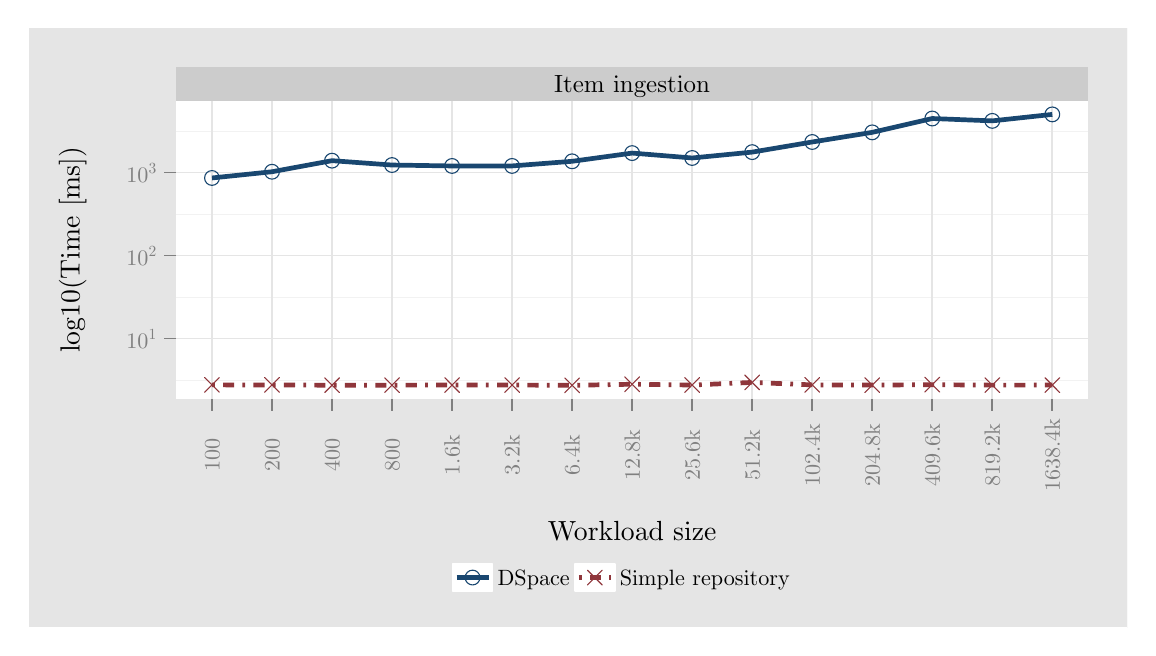
\begin{tikzpicture}[x=1pt,y=1pt]
\definecolor[named]{fillColor}{rgb}{1.00,1.00,1.00}
\path[use as bounding box,fill=fillColor,fill opacity=0.00] (0,0) rectangle (397.48,216.81);
\begin{scope}
\path[clip] (  0.00,  0.00) rectangle (397.48,216.81);
\definecolor[named]{drawColor}{rgb}{1.00,1.00,1.00}
\definecolor[named]{fillColor}{rgb}{0.90,0.90,0.90}

\path[draw=drawColor,line width= 0.6pt,line join=round,line cap=round,fill=fillColor] (  0.00,  0.00) rectangle (397.48,216.81);
\end{scope}
\begin{scope}
\path[clip] ( 53.58, 82.69) rectangle (383.26,190.36);
\definecolor[named]{fillColor}{rgb}{1.00,1.00,1.00}

\path[fill=fillColor] ( 53.58, 82.69) rectangle (383.26,190.36);
\definecolor[named]{drawColor}{rgb}{0.95,0.95,0.95}

\path[draw=drawColor,line width= 0.3pt,line join=round] ( 53.58, 89.48) --
	(383.26, 89.48);

\path[draw=drawColor,line width= 0.3pt,line join=round] ( 53.58,119.46) --
	(383.26,119.46);

\path[draw=drawColor,line width= 0.3pt,line join=round] ( 53.58,149.44) --
	(383.26,149.44);

\path[draw=drawColor,line width= 0.3pt,line join=round] ( 53.58,179.42) --
	(383.26,179.42);
\definecolor[named]{drawColor}{rgb}{0.90,0.90,0.90}

\path[draw=drawColor,line width= 0.6pt,line join=round] ( 53.58,104.47) --
	(383.26,104.47);

\path[draw=drawColor,line width= 0.6pt,line join=round] ( 53.58,134.45) --
	(383.26,134.45);

\path[draw=drawColor,line width= 0.6pt,line join=round] ( 53.58,164.43) --
	(383.26,164.43);

\path[draw=drawColor,line width= 0.6pt,line join=round] ( 66.60, 82.69) --
	( 66.60,190.36);

\path[draw=drawColor,line width= 0.6pt,line join=round] ( 88.29, 82.69) --
	( 88.29,190.36);

\path[draw=drawColor,line width= 0.6pt,line join=round] (109.97, 82.69) --
	(109.97,190.36);

\path[draw=drawColor,line width= 0.6pt,line join=round] (131.66, 82.69) --
	(131.66,190.36);

\path[draw=drawColor,line width= 0.6pt,line join=round] (153.35, 82.69) --
	(153.35,190.36);

\path[draw=drawColor,line width= 0.6pt,line join=round] (175.04, 82.69) --
	(175.04,190.36);

\path[draw=drawColor,line width= 0.6pt,line join=round] (196.73, 82.69) --
	(196.73,190.36);

\path[draw=drawColor,line width= 0.6pt,line join=round] (218.42, 82.69) --
	(218.42,190.36);

\path[draw=drawColor,line width= 0.6pt,line join=round] (240.11, 82.69) --
	(240.11,190.36);

\path[draw=drawColor,line width= 0.6pt,line join=round] (261.80, 82.69) --
	(261.80,190.36);

\path[draw=drawColor,line width= 0.6pt,line join=round] (283.49, 82.69) --
	(283.49,190.36);

\path[draw=drawColor,line width= 0.6pt,line join=round] (305.18, 82.69) --
	(305.18,190.36);

\path[draw=drawColor,line width= 0.6pt,line join=round] (326.87, 82.69) --
	(326.87,190.36);

\path[draw=drawColor,line width= 0.6pt,line join=round] (348.56, 82.69) --
	(348.56,190.36);

\path[draw=drawColor,line width= 0.6pt,line join=round] (370.25, 82.69) --
	(370.25,190.36);
\definecolor[named]{drawColor}{rgb}{0.10,0.28,0.44}

\path[draw=drawColor,line width= 1.7pt,line join=round] ( 66.60,162.50) --
	( 88.29,164.75) --
	(109.97,168.75) --
	(131.66,167.17) --
	(153.35,166.84) --
	(175.04,166.85) --
	(196.73,168.52) --
	(218.42,171.49) --
	(240.11,169.72) --
	(261.80,171.84) --
	(283.49,175.50) --
	(305.18,178.98) --
	(326.87,183.98) --
	(348.56,183.13) --
	(370.25,185.47);
\definecolor[named]{drawColor}{rgb}{0.56,0.21,0.23}

\path[draw=drawColor,line width= 1.7pt,dash pattern=on 1pt off 3pt on 4pt off 3pt ,line join=round] ( 66.60, 87.73) --
	( 88.29, 87.71) --
	(109.97, 87.61) --
	(131.66, 87.63) --
	(153.35, 87.67) --
	(175.04, 87.67) --
	(196.73, 87.58) --
	(218.42, 87.96) --
	(240.11, 87.68) --
	(261.80, 88.62) --
	(283.49, 87.73) --
	(305.18, 87.66) --
	(326.87, 87.80) --
	(348.56, 87.64) --
	(370.25, 87.66);
\definecolor[named]{drawColor}{rgb}{0.10,0.28,0.44}

\path[draw=drawColor,line width= 0.4pt,line join=round,line cap=round] ( 66.60,162.50) circle (  2.67);

\path[draw=drawColor,line width= 0.4pt,line join=round,line cap=round] ( 88.29,164.75) circle (  2.67);

\path[draw=drawColor,line width= 0.4pt,line join=round,line cap=round] (109.97,168.75) circle (  2.67);

\path[draw=drawColor,line width= 0.4pt,line join=round,line cap=round] (131.66,167.17) circle (  2.67);

\path[draw=drawColor,line width= 0.4pt,line join=round,line cap=round] (153.35,166.84) circle (  2.67);

\path[draw=drawColor,line width= 0.4pt,line join=round,line cap=round] (175.04,166.85) circle (  2.67);

\path[draw=drawColor,line width= 0.4pt,line join=round,line cap=round] (196.73,168.52) circle (  2.67);

\path[draw=drawColor,line width= 0.4pt,line join=round,line cap=round] (218.42,171.49) circle (  2.67);

\path[draw=drawColor,line width= 0.4pt,line join=round,line cap=round] (240.11,169.72) circle (  2.67);

\path[draw=drawColor,line width= 0.4pt,line join=round,line cap=round] (261.80,171.84) circle (  2.67);

\path[draw=drawColor,line width= 0.4pt,line join=round,line cap=round] (283.49,175.50) circle (  2.67);

\path[draw=drawColor,line width= 0.4pt,line join=round,line cap=round] (305.18,178.98) circle (  2.67);

\path[draw=drawColor,line width= 0.4pt,line join=round,line cap=round] (326.87,183.98) circle (  2.67);

\path[draw=drawColor,line width= 0.4pt,line join=round,line cap=round] (348.56,183.13) circle (  2.67);

\path[draw=drawColor,line width= 0.4pt,line join=round,line cap=round] (370.25,185.47) circle (  2.67);
\definecolor[named]{drawColor}{rgb}{0.56,0.21,0.23}

\path[draw=drawColor,line width= 0.4pt,line join=round,line cap=round,fill=fillColor] ( 63.93, 85.06) -- ( 69.26, 90.39);

\path[draw=drawColor,line width= 0.4pt,line join=round,line cap=round,fill=fillColor] ( 63.93, 90.39) -- ( 69.26, 85.06);

\path[draw=drawColor,line width= 0.4pt,line join=round,line cap=round,fill=fillColor] ( 85.62, 85.04) -- ( 90.95, 90.38);

\path[draw=drawColor,line width= 0.4pt,line join=round,line cap=round,fill=fillColor] ( 85.62, 90.38) -- ( 90.95, 85.04);

\path[draw=drawColor,line width= 0.4pt,line join=round,line cap=round,fill=fillColor] (107.31, 84.94) -- (112.64, 90.28);

\path[draw=drawColor,line width= 0.4pt,line join=round,line cap=round,fill=fillColor] (107.31, 90.28) -- (112.64, 84.94);

\path[draw=drawColor,line width= 0.4pt,line join=round,line cap=round,fill=fillColor] (129.00, 84.97) -- (134.33, 90.30);

\path[draw=drawColor,line width= 0.4pt,line join=round,line cap=round,fill=fillColor] (129.00, 90.30) -- (134.33, 84.97);

\path[draw=drawColor,line width= 0.4pt,line join=round,line cap=round,fill=fillColor] (150.69, 85.00) -- (156.02, 90.34);

\path[draw=drawColor,line width= 0.4pt,line join=round,line cap=round,fill=fillColor] (150.69, 90.34) -- (156.02, 85.00);

\path[draw=drawColor,line width= 0.4pt,line join=round,line cap=round,fill=fillColor] (172.37, 85.00) -- (177.71, 90.34);

\path[draw=drawColor,line width= 0.4pt,line join=round,line cap=round,fill=fillColor] (172.37, 90.34) -- (177.71, 85.00);

\path[draw=drawColor,line width= 0.4pt,line join=round,line cap=round,fill=fillColor] (194.06, 84.92) -- (199.40, 90.25);

\path[draw=drawColor,line width= 0.4pt,line join=round,line cap=round,fill=fillColor] (194.06, 90.25) -- (199.40, 84.92);

\path[draw=drawColor,line width= 0.4pt,line join=round,line cap=round,fill=fillColor] (215.75, 85.29) -- (221.09, 90.62);

\path[draw=drawColor,line width= 0.4pt,line join=round,line cap=round,fill=fillColor] (215.75, 90.62) -- (221.09, 85.29);

\path[draw=drawColor,line width= 0.4pt,line join=round,line cap=round,fill=fillColor] (237.44, 85.02) -- (242.78, 90.35);

\path[draw=drawColor,line width= 0.4pt,line join=round,line cap=round,fill=fillColor] (237.44, 90.35) -- (242.78, 85.02);

\path[draw=drawColor,line width= 0.4pt,line join=round,line cap=round,fill=fillColor] (259.13, 85.95) -- (264.47, 91.29);

\path[draw=drawColor,line width= 0.4pt,line join=round,line cap=round,fill=fillColor] (259.13, 91.29) -- (264.47, 85.95);

\path[draw=drawColor,line width= 0.4pt,line join=round,line cap=round,fill=fillColor] (280.82, 85.06) -- (286.16, 90.40);

\path[draw=drawColor,line width= 0.4pt,line join=round,line cap=round,fill=fillColor] (280.82, 90.40) -- (286.16, 85.06);

\path[draw=drawColor,line width= 0.4pt,line join=round,line cap=round,fill=fillColor] (302.51, 84.99) -- (307.84, 90.33);

\path[draw=drawColor,line width= 0.4pt,line join=round,line cap=round,fill=fillColor] (302.51, 90.33) -- (307.84, 84.99);

\path[draw=drawColor,line width= 0.4pt,line join=round,line cap=round,fill=fillColor] (324.20, 85.13) -- (329.53, 90.47);

\path[draw=drawColor,line width= 0.4pt,line join=round,line cap=round,fill=fillColor] (324.20, 90.47) -- (329.53, 85.13);

\path[draw=drawColor,line width= 0.4pt,line join=round,line cap=round,fill=fillColor] (345.89, 84.97) -- (351.22, 90.31);

\path[draw=drawColor,line width= 0.4pt,line join=round,line cap=round,fill=fillColor] (345.89, 90.31) -- (351.22, 84.97);

\path[draw=drawColor,line width= 0.4pt,line join=round,line cap=round,fill=fillColor] (367.58, 84.99) -- (372.91, 90.33);

\path[draw=drawColor,line width= 0.4pt,line join=round,line cap=round,fill=fillColor] (367.58, 90.33) -- (372.91, 84.99);
\end{scope}
\begin{scope}
\path[clip] (  0.00,  0.00) rectangle (397.48,216.81);
\definecolor[named]{fillColor}{rgb}{0.80,0.80,0.80}

\path[fill=fillColor] ( 53.58,190.36) rectangle (383.26,202.58);
\definecolor[named]{drawColor}{rgb}{0.00,0.00,0.00}

\node[text=drawColor,anchor=base,inner sep=0pt, outer sep=0pt, scale=  0.90] at (218.42,193.37) {Item ingestion};
\end{scope}
\begin{scope}
\path[clip] (  0.00,  0.00) rectangle (397.48,216.81);
\definecolor[named]{drawColor}{rgb}{0.50,0.50,0.50}

\node[text=drawColor,anchor=base west,inner sep=0pt, outer sep=0pt, scale=  0.80] at ( 35.67,101.04) {10};

\node[text=drawColor,anchor=base west,inner sep=0pt, outer sep=0pt, scale=  0.56] at ( 43.67,104.31) {1};

\node[text=drawColor,anchor=base west,inner sep=0pt, outer sep=0pt, scale=  0.80] at ( 35.67,131.02) {10};

\node[text=drawColor,anchor=base west,inner sep=0pt, outer sep=0pt, scale=  0.56] at ( 43.67,134.29) {2};

\node[text=drawColor,anchor=base west,inner sep=0pt, outer sep=0pt, scale=  0.80] at ( 35.67,161.00) {10};

\node[text=drawColor,anchor=base west,inner sep=0pt, outer sep=0pt, scale=  0.56] at ( 43.67,164.27) {3};
\end{scope}
\begin{scope}
\path[clip] (  0.00,  0.00) rectangle (397.48,216.81);
\definecolor[named]{drawColor}{rgb}{0.50,0.50,0.50}

\path[draw=drawColor,line width= 0.6pt,line join=round] ( 49.31,104.47) --
	( 53.58,104.47);

\path[draw=drawColor,line width= 0.6pt,line join=round] ( 49.31,134.45) --
	( 53.58,134.45);

\path[draw=drawColor,line width= 0.6pt,line join=round] ( 49.31,164.43) --
	( 53.58,164.43);
\end{scope}
\begin{scope}
\path[clip] (  0.00,  0.00) rectangle (397.48,216.81);
\definecolor[named]{drawColor}{rgb}{0.50,0.50,0.50}

\path[draw=drawColor,line width= 0.6pt,line join=round] ( 66.60, 78.42) --
	( 66.60, 82.69);

\path[draw=drawColor,line width= 0.6pt,line join=round] ( 88.29, 78.42) --
	( 88.29, 82.69);

\path[draw=drawColor,line width= 0.6pt,line join=round] (109.97, 78.42) --
	(109.97, 82.69);

\path[draw=drawColor,line width= 0.6pt,line join=round] (131.66, 78.42) --
	(131.66, 82.69);

\path[draw=drawColor,line width= 0.6pt,line join=round] (153.35, 78.42) --
	(153.35, 82.69);

\path[draw=drawColor,line width= 0.6pt,line join=round] (175.04, 78.42) --
	(175.04, 82.69);

\path[draw=drawColor,line width= 0.6pt,line join=round] (196.73, 78.42) --
	(196.73, 82.69);

\path[draw=drawColor,line width= 0.6pt,line join=round] (218.42, 78.42) --
	(218.42, 82.69);

\path[draw=drawColor,line width= 0.6pt,line join=round] (240.11, 78.42) --
	(240.11, 82.69);

\path[draw=drawColor,line width= 0.6pt,line join=round] (261.80, 78.42) --
	(261.80, 82.69);

\path[draw=drawColor,line width= 0.6pt,line join=round] (283.49, 78.42) --
	(283.49, 82.69);

\path[draw=drawColor,line width= 0.6pt,line join=round] (305.18, 78.42) --
	(305.18, 82.69);

\path[draw=drawColor,line width= 0.6pt,line join=round] (326.87, 78.42) --
	(326.87, 82.69);

\path[draw=drawColor,line width= 0.6pt,line join=round] (348.56, 78.42) --
	(348.56, 82.69);

\path[draw=drawColor,line width= 0.6pt,line join=round] (370.25, 78.42) --
	(370.25, 82.69);
\end{scope}
\begin{scope}
\path[clip] (  0.00,  0.00) rectangle (397.48,216.81);
\definecolor[named]{drawColor}{rgb}{0.50,0.50,0.50}

\node[text=drawColor,rotate= 90.00,anchor=base,inner sep=0pt, outer sep=0pt, scale=  0.80] at ( 69.35, 62.36) {100};

\node[text=drawColor,rotate= 90.00,anchor=base,inner sep=0pt, outer sep=0pt, scale=  0.80] at ( 91.04, 62.36) {200};

\node[text=drawColor,rotate= 90.00,anchor=base,inner sep=0pt, outer sep=0pt, scale=  0.80] at (112.73, 62.36) {400};

\node[text=drawColor,rotate= 90.00,anchor=base,inner sep=0pt, outer sep=0pt, scale=  0.80] at (134.42, 62.36) {800};

\node[text=drawColor,rotate= 90.00,anchor=base,inner sep=0pt, outer sep=0pt, scale=  0.80] at (156.11, 62.36) {1.6k};

\node[text=drawColor,rotate= 90.00,anchor=base,inner sep=0pt, outer sep=0pt, scale=  0.80] at (177.80, 62.36) {3.2k};

\node[text=drawColor,rotate= 90.00,anchor=base,inner sep=0pt, outer sep=0pt, scale=  0.80] at (199.49, 62.36) {6.4k};

\node[text=drawColor,rotate= 90.00,anchor=base,inner sep=0pt, outer sep=0pt, scale=  0.80] at (221.18, 62.36) {12.8k};

\node[text=drawColor,rotate= 90.00,anchor=base,inner sep=0pt, outer sep=0pt, scale=  0.80] at (242.86, 62.36) {25.6k};

\node[text=drawColor,rotate= 90.00,anchor=base,inner sep=0pt, outer sep=0pt, scale=  0.80] at (264.55, 62.36) {51.2k};

\node[text=drawColor,rotate= 90.00,anchor=base,inner sep=0pt, outer sep=0pt, scale=  0.80] at (286.24, 62.36) {102.4k};

\node[text=drawColor,rotate= 90.00,anchor=base,inner sep=0pt, outer sep=0pt, scale=  0.80] at (307.93, 62.36) {204.8k};

\node[text=drawColor,rotate= 90.00,anchor=base,inner sep=0pt, outer sep=0pt, scale=  0.80] at (329.62, 62.36) {409.6k};

\node[text=drawColor,rotate= 90.00,anchor=base,inner sep=0pt, outer sep=0pt, scale=  0.80] at (351.31, 62.36) {819.2k};

\node[text=drawColor,rotate= 90.00,anchor=base,inner sep=0pt, outer sep=0pt, scale=  0.80] at (373.00, 62.36) {1638.4k};
\end{scope}
\begin{scope}
\path[clip] (  0.00,  0.00) rectangle (397.48,216.81);
\definecolor[named]{drawColor}{rgb}{0.00,0.00,0.00}

\node[text=drawColor,anchor=base,inner sep=0pt, outer sep=0pt, scale=  1.00] at (218.42, 31.41) {Workload size};
\end{scope}
\begin{scope}
\path[clip] (  0.00,  0.00) rectangle (397.48,216.81);
\definecolor[named]{drawColor}{rgb}{0.00,0.00,0.00}

\node[text=drawColor,rotate= 90.00,anchor=base,inner sep=0pt, outer sep=0pt, scale=  1.00] at ( 18.80,136.53) {log10(Time [ms])};
\end{scope}
\begin{scope}
\path[clip] (  0.00,  0.00) rectangle (397.48,216.81);
\definecolor[named]{fillColor}{rgb}{0.90,0.90,0.90}

\path[fill=fillColor] (145.65,  8.87) rectangle (291.19, 27.36);
\end{scope}
\begin{scope}
\path[clip] (  0.00,  0.00) rectangle (397.48,216.81);
\definecolor[named]{drawColor}{rgb}{1.00,1.00,1.00}
\definecolor[named]{fillColor}{rgb}{1.00,1.00,1.00}

\path[draw=drawColor,line width= 0.6pt,line join=round,line cap=round,fill=fillColor] (153.53, 13.14) rectangle (167.98, 23.09);
\end{scope}
\begin{scope}
\path[clip] (  0.00,  0.00) rectangle (397.48,216.81);
\definecolor[named]{drawColor}{rgb}{0.10,0.28,0.44}

\path[draw=drawColor,line width= 1.7pt,line join=round] (154.98, 18.11) -- (166.54, 18.11);
\end{scope}
\begin{scope}
\path[clip] (  0.00,  0.00) rectangle (397.48,216.81);
\definecolor[named]{drawColor}{rgb}{0.10,0.28,0.44}

\path[draw=drawColor,line width= 0.4pt,line join=round,line cap=round] (160.76, 18.11) circle (  2.67);
\end{scope}
\begin{scope}
\path[clip] (  0.00,  0.00) rectangle (397.48,216.81);
\definecolor[named]{drawColor}{rgb}{1.00,1.00,1.00}
\definecolor[named]{fillColor}{rgb}{1.00,1.00,1.00}

\path[draw=drawColor,line width= 0.6pt,line join=round,line cap=round,fill=fillColor] (197.70, 13.14) rectangle (212.16, 23.09);
\end{scope}
\begin{scope}
\path[clip] (  0.00,  0.00) rectangle (397.48,216.81);
\definecolor[named]{drawColor}{rgb}{0.56,0.21,0.23}

\path[draw=drawColor,line width= 1.7pt,dash pattern=on 1pt off 3pt on 4pt off 3pt ,line join=round] (199.15, 18.11) -- (210.71, 18.11);
\end{scope}
\begin{scope}
\path[clip] (  0.00,  0.00) rectangle (397.48,216.81);
\definecolor[named]{drawColor}{rgb}{0.56,0.21,0.23}
\definecolor[named]{fillColor}{rgb}{1.00,1.00,1.00}

\path[draw=drawColor,line width= 0.4pt,line join=round,line cap=round,fill=fillColor] (202.26, 15.45) -- (207.60, 20.78);

\path[draw=drawColor,line width= 0.4pt,line join=round,line cap=round,fill=fillColor] (202.26, 20.78) -- (207.60, 15.45);
\end{scope}
\begin{scope}
\path[clip] (  0.00,  0.00) rectangle (397.48,216.81);
\definecolor[named]{drawColor}{rgb}{0.00,0.00,0.00}

\node[text=drawColor,anchor=base west,inner sep=0pt, outer sep=0pt, scale=  0.80] at (169.79, 15.36) {DSpace};
\end{scope}
\begin{scope}
\path[clip] (  0.00,  0.00) rectangle (397.48,216.81);
\definecolor[named]{drawColor}{rgb}{0.00,0.00,0.00}

\node[text=drawColor,anchor=base west,inner sep=0pt, outer sep=0pt, scale=  0.80] at (213.96, 15.36) {Simple repository $\;\;\;\;$};
\end{scope}
\end{tikzpicture}

 }
\caption[Comparison of single item ingestion\index{Ingestion} performance]{A plot showing a comparison of ingestion\index{Ingestion} performance between the simple repository and DSpace.}
 \label{fig:experimentation:performance:comparision:ingest}
\end{figure}

\begin{figure}
 \centering
 \framebox[\textwidth]{%
% Created by tikzDevice version 0.6.2-92-0ad2792 on 2013-04-07 18:10:31
% !TEX encoding = UTF-8 Unicode
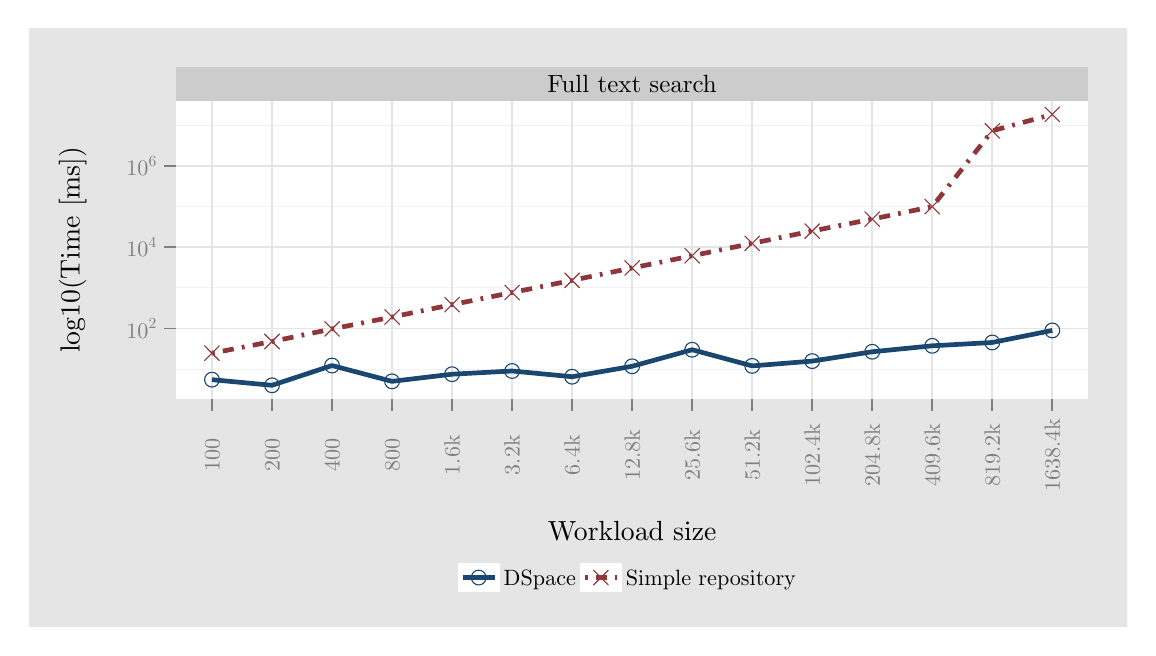
\begin{tikzpicture}[x=1pt,y=1pt]
\definecolor[named]{fillColor}{rgb}{1.00,1.00,1.00}
\path[use as bounding box,fill=fillColor,fill opacity=0.00] (0,0) rectangle (397.48,216.81);
\begin{scope}
\path[clip] (  0.00,  0.00) rectangle (397.48,216.81);
\definecolor[named]{drawColor}{rgb}{1.00,1.00,1.00}
\definecolor[named]{fillColor}{rgb}{0.90,0.90,0.90}

\path[draw=drawColor,line width= 0.6pt,line join=round,line cap=round,fill=fillColor] (  0.00,  0.00) rectangle (397.48,216.81);
\end{scope}
\begin{scope}
\path[clip] ( 53.58, 82.69) rectangle (383.26,190.36);
\definecolor[named]{fillColor}{rgb}{1.00,1.00,1.00}

\path[fill=fillColor] ( 53.58, 82.69) rectangle (383.26,190.36);
\definecolor[named]{drawColor}{rgb}{0.95,0.95,0.95}

\path[draw=drawColor,line width= 0.3pt,line join=round] ( 53.58, 93.43) --
	(383.26, 93.43);

\path[draw=drawColor,line width= 0.3pt,line join=round] ( 53.58,122.78) --
	(383.26,122.78);

\path[draw=drawColor,line width= 0.3pt,line join=round] ( 53.58,152.14) --
	(383.26,152.14);

\path[draw=drawColor,line width= 0.3pt,line join=round] ( 53.58,181.49) --
	(383.26,181.49);
\definecolor[named]{drawColor}{rgb}{0.90,0.90,0.90}

\path[draw=drawColor,line width= 0.6pt,line join=round] ( 53.58,108.10) --
	(383.26,108.10);

\path[draw=drawColor,line width= 0.6pt,line join=round] ( 53.58,137.46) --
	(383.26,137.46);

\path[draw=drawColor,line width= 0.6pt,line join=round] ( 53.58,166.81) --
	(383.26,166.81);

\path[draw=drawColor,line width= 0.6pt,line join=round] ( 66.60, 82.69) --
	( 66.60,190.36);

\path[draw=drawColor,line width= 0.6pt,line join=round] ( 88.29, 82.69) --
	( 88.29,190.36);

\path[draw=drawColor,line width= 0.6pt,line join=round] (109.97, 82.69) --
	(109.97,190.36);

\path[draw=drawColor,line width= 0.6pt,line join=round] (131.66, 82.69) --
	(131.66,190.36);

\path[draw=drawColor,line width= 0.6pt,line join=round] (153.35, 82.69) --
	(153.35,190.36);

\path[draw=drawColor,line width= 0.6pt,line join=round] (175.04, 82.69) --
	(175.04,190.36);

\path[draw=drawColor,line width= 0.6pt,line join=round] (196.73, 82.69) --
	(196.73,190.36);

\path[draw=drawColor,line width= 0.6pt,line join=round] (218.42, 82.69) --
	(218.42,190.36);

\path[draw=drawColor,line width= 0.6pt,line join=round] (240.11, 82.69) --
	(240.11,190.36);

\path[draw=drawColor,line width= 0.6pt,line join=round] (261.80, 82.69) --
	(261.80,190.36);

\path[draw=drawColor,line width= 0.6pt,line join=round] (283.49, 82.69) --
	(283.49,190.36);

\path[draw=drawColor,line width= 0.6pt,line join=round] (305.18, 82.69) --
	(305.18,190.36);

\path[draw=drawColor,line width= 0.6pt,line join=round] (326.87, 82.69) --
	(326.87,190.36);

\path[draw=drawColor,line width= 0.6pt,line join=round] (348.56, 82.69) --
	(348.56,190.36);

\path[draw=drawColor,line width= 0.6pt,line join=round] (370.25, 82.69) --
	(370.25,190.36);
\definecolor[named]{drawColor}{rgb}{0.10,0.28,0.44}

\path[draw=drawColor,line width= 1.7pt,line join=round] ( 66.60, 89.61) --
	( 88.29, 87.58) --
	(109.97, 94.72) --
	(131.66, 89.01) --
	(153.35, 91.59) --
	(175.04, 92.75) --
	(196.73, 90.68) --
	(218.42, 94.45) --
	(240.11,100.43) --
	(261.80, 94.59) --
	(283.49, 96.32) --
	(305.18, 99.70) --
	(326.87,101.85) --
	(348.56,103.05) --
	(370.25,107.41);
\definecolor[named]{drawColor}{rgb}{0.56,0.21,0.23}

\path[draw=drawColor,line width= 1.7pt,dash pattern=on 1pt off 3pt on 4pt off 3pt ,line join=round] ( 66.60, 99.18) --
	( 88.29,103.41) --
	(109.97,107.93) --
	(131.66,112.26) --
	(153.35,116.73) --
	(175.04,121.10) --
	(196.73,125.50) --
	(218.42,129.98) --
	(240.11,134.38) --
	(261.80,138.87) --
	(283.49,143.33) --
	(305.18,147.63) --
	(326.87,152.15) --
	(348.56,179.54) --
	(370.25,185.47);
\definecolor[named]{drawColor}{rgb}{0.10,0.28,0.44}

\path[draw=drawColor,line width= 0.4pt,line join=round,line cap=round] ( 66.60, 89.61) circle (  2.67);

\path[draw=drawColor,line width= 0.4pt,line join=round,line cap=round] ( 88.29, 87.58) circle (  2.67);

\path[draw=drawColor,line width= 0.4pt,line join=round,line cap=round] (109.97, 94.72) circle (  2.67);

\path[draw=drawColor,line width= 0.4pt,line join=round,line cap=round] (131.66, 89.01) circle (  2.67);

\path[draw=drawColor,line width= 0.4pt,line join=round,line cap=round] (153.35, 91.59) circle (  2.67);

\path[draw=drawColor,line width= 0.4pt,line join=round,line cap=round] (175.04, 92.75) circle (  2.67);

\path[draw=drawColor,line width= 0.4pt,line join=round,line cap=round] (196.73, 90.68) circle (  2.67);

\path[draw=drawColor,line width= 0.4pt,line join=round,line cap=round] (218.42, 94.45) circle (  2.67);

\path[draw=drawColor,line width= 0.4pt,line join=round,line cap=round] (240.11,100.43) circle (  2.67);

\path[draw=drawColor,line width= 0.4pt,line join=round,line cap=round] (261.80, 94.59) circle (  2.67);

\path[draw=drawColor,line width= 0.4pt,line join=round,line cap=round] (283.49, 96.32) circle (  2.67);

\path[draw=drawColor,line width= 0.4pt,line join=round,line cap=round] (305.18, 99.70) circle (  2.67);

\path[draw=drawColor,line width= 0.4pt,line join=round,line cap=round] (326.87,101.85) circle (  2.67);

\path[draw=drawColor,line width= 0.4pt,line join=round,line cap=round] (348.56,103.05) circle (  2.67);

\path[draw=drawColor,line width= 0.4pt,line join=round,line cap=round] (370.25,107.41) circle (  2.67);
\definecolor[named]{drawColor}{rgb}{0.56,0.21,0.23}

\path[draw=drawColor,line width= 0.4pt,line join=round,line cap=round,fill=fillColor] ( 63.93, 96.51) -- ( 69.26,101.85);

\path[draw=drawColor,line width= 0.4pt,line join=round,line cap=round,fill=fillColor] ( 63.93,101.85) -- ( 69.26, 96.51);

\path[draw=drawColor,line width= 0.4pt,line join=round,line cap=round,fill=fillColor] ( 85.62,100.74) -- ( 90.95,106.08);

\path[draw=drawColor,line width= 0.4pt,line join=round,line cap=round,fill=fillColor] ( 85.62,106.08) -- ( 90.95,100.74);

\path[draw=drawColor,line width= 0.4pt,line join=round,line cap=round,fill=fillColor] (107.31,105.27) -- (112.64,110.60);

\path[draw=drawColor,line width= 0.4pt,line join=round,line cap=round,fill=fillColor] (107.31,110.60) -- (112.64,105.27);

\path[draw=drawColor,line width= 0.4pt,line join=round,line cap=round,fill=fillColor] (129.00,109.59) -- (134.33,114.93);

\path[draw=drawColor,line width= 0.4pt,line join=round,line cap=round,fill=fillColor] (129.00,114.93) -- (134.33,109.59);

\path[draw=drawColor,line width= 0.4pt,line join=round,line cap=round,fill=fillColor] (150.69,114.06) -- (156.02,119.40);

\path[draw=drawColor,line width= 0.4pt,line join=round,line cap=round,fill=fillColor] (150.69,119.40) -- (156.02,114.06);

\path[draw=drawColor,line width= 0.4pt,line join=round,line cap=round,fill=fillColor] (172.37,118.43) -- (177.71,123.77);

\path[draw=drawColor,line width= 0.4pt,line join=round,line cap=round,fill=fillColor] (172.37,123.77) -- (177.71,118.43);

\path[draw=drawColor,line width= 0.4pt,line join=round,line cap=round,fill=fillColor] (194.06,122.83) -- (199.40,128.16);

\path[draw=drawColor,line width= 0.4pt,line join=round,line cap=round,fill=fillColor] (194.06,128.16) -- (199.40,122.83);

\path[draw=drawColor,line width= 0.4pt,line join=round,line cap=round,fill=fillColor] (215.75,127.31) -- (221.09,132.65);

\path[draw=drawColor,line width= 0.4pt,line join=round,line cap=round,fill=fillColor] (215.75,132.65) -- (221.09,127.31);

\path[draw=drawColor,line width= 0.4pt,line join=round,line cap=round,fill=fillColor] (237.44,131.71) -- (242.78,137.05);

\path[draw=drawColor,line width= 0.4pt,line join=round,line cap=round,fill=fillColor] (237.44,137.05) -- (242.78,131.71);

\path[draw=drawColor,line width= 0.4pt,line join=round,line cap=round,fill=fillColor] (259.13,136.21) -- (264.47,141.54);

\path[draw=drawColor,line width= 0.4pt,line join=round,line cap=round,fill=fillColor] (259.13,141.54) -- (264.47,136.21);

\path[draw=drawColor,line width= 0.4pt,line join=round,line cap=round,fill=fillColor] (280.82,140.66) -- (286.16,145.99);

\path[draw=drawColor,line width= 0.4pt,line join=round,line cap=round,fill=fillColor] (280.82,145.99) -- (286.16,140.66);

\path[draw=drawColor,line width= 0.4pt,line join=round,line cap=round,fill=fillColor] (302.51,144.96) -- (307.84,150.30);

\path[draw=drawColor,line width= 0.4pt,line join=round,line cap=round,fill=fillColor] (302.51,150.30) -- (307.84,144.96);

\path[draw=drawColor,line width= 0.4pt,line join=round,line cap=round,fill=fillColor] (324.20,149.49) -- (329.53,154.82);

\path[draw=drawColor,line width= 0.4pt,line join=round,line cap=round,fill=fillColor] (324.20,154.82) -- (329.53,149.49);

\path[draw=drawColor,line width= 0.4pt,line join=round,line cap=round,fill=fillColor] (345.89,176.87) -- (351.22,182.21);

\path[draw=drawColor,line width= 0.4pt,line join=round,line cap=round,fill=fillColor] (345.89,182.21) -- (351.22,176.87);

\path[draw=drawColor,line width= 0.4pt,line join=round,line cap=round,fill=fillColor] (367.58,182.80) -- (372.91,188.14);

\path[draw=drawColor,line width= 0.4pt,line join=round,line cap=round,fill=fillColor] (367.58,188.14) -- (372.91,182.80);
\end{scope}
\begin{scope}
\path[clip] (  0.00,  0.00) rectangle (397.48,216.81);
\definecolor[named]{fillColor}{rgb}{0.80,0.80,0.80}

\path[fill=fillColor] ( 53.58,190.36) rectangle (383.26,202.58);
\definecolor[named]{drawColor}{rgb}{0.00,0.00,0.00}

\node[text=drawColor,anchor=base,inner sep=0pt, outer sep=0pt, scale=  0.90] at (218.42,193.37) {Full text search};
\end{scope}
\begin{scope}
\path[clip] (  0.00,  0.00) rectangle (397.48,216.81);
\definecolor[named]{drawColor}{rgb}{0.50,0.50,0.50}

\node[text=drawColor,anchor=base west,inner sep=0pt, outer sep=0pt, scale=  0.80] at ( 35.67,104.67) {10};

\node[text=drawColor,anchor=base west,inner sep=0pt, outer sep=0pt, scale=  0.56] at ( 43.67,107.94) {2};

\node[text=drawColor,anchor=base west,inner sep=0pt, outer sep=0pt, scale=  0.80] at ( 35.67,134.03) {10};

\node[text=drawColor,anchor=base west,inner sep=0pt, outer sep=0pt, scale=  0.56] at ( 43.67,137.30) {4};

\node[text=drawColor,anchor=base west,inner sep=0pt, outer sep=0pt, scale=  0.80] at ( 35.67,163.38) {10};

\node[text=drawColor,anchor=base west,inner sep=0pt, outer sep=0pt, scale=  0.56] at ( 43.67,166.65) {6};
\end{scope}
\begin{scope}
\path[clip] (  0.00,  0.00) rectangle (397.48,216.81);
\definecolor[named]{drawColor}{rgb}{0.50,0.50,0.50}

\path[draw=drawColor,line width= 0.6pt,line join=round] ( 49.31,108.10) --
	( 53.58,108.10);

\path[draw=drawColor,line width= 0.6pt,line join=round] ( 49.31,137.46) --
	( 53.58,137.46);

\path[draw=drawColor,line width= 0.6pt,line join=round] ( 49.31,166.81) --
	( 53.58,166.81);
\end{scope}
\begin{scope}
\path[clip] (  0.00,  0.00) rectangle (397.48,216.81);
\definecolor[named]{drawColor}{rgb}{0.50,0.50,0.50}

\path[draw=drawColor,line width= 0.6pt,line join=round] ( 66.60, 78.42) --
	( 66.60, 82.69);

\path[draw=drawColor,line width= 0.6pt,line join=round] ( 88.29, 78.42) --
	( 88.29, 82.69);

\path[draw=drawColor,line width= 0.6pt,line join=round] (109.97, 78.42) --
	(109.97, 82.69);

\path[draw=drawColor,line width= 0.6pt,line join=round] (131.66, 78.42) --
	(131.66, 82.69);

\path[draw=drawColor,line width= 0.6pt,line join=round] (153.35, 78.42) --
	(153.35, 82.69);

\path[draw=drawColor,line width= 0.6pt,line join=round] (175.04, 78.42) --
	(175.04, 82.69);

\path[draw=drawColor,line width= 0.6pt,line join=round] (196.73, 78.42) --
	(196.73, 82.69);

\path[draw=drawColor,line width= 0.6pt,line join=round] (218.42, 78.42) --
	(218.42, 82.69);

\path[draw=drawColor,line width= 0.6pt,line join=round] (240.11, 78.42) --
	(240.11, 82.69);

\path[draw=drawColor,line width= 0.6pt,line join=round] (261.80, 78.42) --
	(261.80, 82.69);

\path[draw=drawColor,line width= 0.6pt,line join=round] (283.49, 78.42) --
	(283.49, 82.69);

\path[draw=drawColor,line width= 0.6pt,line join=round] (305.18, 78.42) --
	(305.18, 82.69);

\path[draw=drawColor,line width= 0.6pt,line join=round] (326.87, 78.42) --
	(326.87, 82.69);

\path[draw=drawColor,line width= 0.6pt,line join=round] (348.56, 78.42) --
	(348.56, 82.69);

\path[draw=drawColor,line width= 0.6pt,line join=round] (370.25, 78.42) --
	(370.25, 82.69);
\end{scope}
\begin{scope}
\path[clip] (  0.00,  0.00) rectangle (397.48,216.81);
\definecolor[named]{drawColor}{rgb}{0.50,0.50,0.50}

\node[text=drawColor,rotate= 90.00,anchor=base,inner sep=0pt, outer sep=0pt, scale=  0.80] at ( 69.35, 62.36) {100};

\node[text=drawColor,rotate= 90.00,anchor=base,inner sep=0pt, outer sep=0pt, scale=  0.80] at ( 91.04, 62.36) {200};

\node[text=drawColor,rotate= 90.00,anchor=base,inner sep=0pt, outer sep=0pt, scale=  0.80] at (112.73, 62.36) {400};

\node[text=drawColor,rotate= 90.00,anchor=base,inner sep=0pt, outer sep=0pt, scale=  0.80] at (134.42, 62.36) {800};

\node[text=drawColor,rotate= 90.00,anchor=base,inner sep=0pt, outer sep=0pt, scale=  0.80] at (156.11, 62.36) {1.6k};

\node[text=drawColor,rotate= 90.00,anchor=base,inner sep=0pt, outer sep=0pt, scale=  0.80] at (177.80, 62.36) {3.2k};

\node[text=drawColor,rotate= 90.00,anchor=base,inner sep=0pt, outer sep=0pt, scale=  0.80] at (199.49, 62.36) {6.4k};

\node[text=drawColor,rotate= 90.00,anchor=base,inner sep=0pt, outer sep=0pt, scale=  0.80] at (221.18, 62.36) {12.8k};

\node[text=drawColor,rotate= 90.00,anchor=base,inner sep=0pt, outer sep=0pt, scale=  0.80] at (242.86, 62.36) {25.6k};

\node[text=drawColor,rotate= 90.00,anchor=base,inner sep=0pt, outer sep=0pt, scale=  0.80] at (264.55, 62.36) {51.2k};

\node[text=drawColor,rotate= 90.00,anchor=base,inner sep=0pt, outer sep=0pt, scale=  0.80] at (286.24, 62.36) {102.4k};

\node[text=drawColor,rotate= 90.00,anchor=base,inner sep=0pt, outer sep=0pt, scale=  0.80] at (307.93, 62.36) {204.8k};

\node[text=drawColor,rotate= 90.00,anchor=base,inner sep=0pt, outer sep=0pt, scale=  0.80] at (329.62, 62.36) {409.6k};

\node[text=drawColor,rotate= 90.00,anchor=base,inner sep=0pt, outer sep=0pt, scale=  0.80] at (351.31, 62.36) {819.2k};

\node[text=drawColor,rotate= 90.00,anchor=base,inner sep=0pt, outer sep=0pt, scale=  0.80] at (373.00, 62.36) {1638.4k};
\end{scope}
\begin{scope}
\path[clip] (  0.00,  0.00) rectangle (397.48,216.81);
\definecolor[named]{drawColor}{rgb}{0.00,0.00,0.00}

\node[text=drawColor,anchor=base,inner sep=0pt, outer sep=0pt, scale=  1.00] at (218.42, 31.41) {Workload size};
\end{scope}
\begin{scope}
\path[clip] (  0.00,  0.00) rectangle (397.48,216.81);
\definecolor[named]{drawColor}{rgb}{0.00,0.00,0.00}

\node[text=drawColor,rotate= 90.00,anchor=base,inner sep=0pt, outer sep=0pt, scale=  1.00] at ( 18.80,136.53) {log10(Time [ms])};
\end{scope}
\begin{scope}
\path[clip] (  0.00,  0.00) rectangle (397.48,216.81);
\definecolor[named]{fillColor}{rgb}{0.90,0.90,0.90}

\path[fill=fillColor] (147.87,  8.87) rectangle (288.97, 27.36);
\end{scope}
\begin{scope}
\path[clip] (  0.00,  0.00) rectangle (397.48,216.81);
\definecolor[named]{drawColor}{rgb}{1.00,1.00,1.00}
\definecolor[named]{fillColor}{rgb}{1.00,1.00,1.00}

\path[draw=drawColor,line width= 0.6pt,line join=round,line cap=round,fill=fillColor] (155.75, 13.14) rectangle (170.21, 23.09);
\end{scope}
\begin{scope}
\path[clip] (  0.00,  0.00) rectangle (397.48,216.81);
\definecolor[named]{drawColor}{rgb}{0.10,0.28,0.44}

\path[draw=drawColor,line width= 1.7pt,line join=round] (157.20, 18.11) -- (168.76, 18.11);
\end{scope}
\begin{scope}
\path[clip] (  0.00,  0.00) rectangle (397.48,216.81);
\definecolor[named]{drawColor}{rgb}{0.10,0.28,0.44}

\path[draw=drawColor,line width= 0.4pt,line join=round,line cap=round] (162.98, 18.11) circle (  2.67);
\end{scope}
\begin{scope}
\path[clip] (  0.00,  0.00) rectangle (397.48,216.81);
\definecolor[named]{drawColor}{rgb}{1.00,1.00,1.00}
\definecolor[named]{fillColor}{rgb}{1.00,1.00,1.00}

\path[draw=drawColor,line width= 0.6pt,line join=round,line cap=round,fill=fillColor] (199.92, 13.14) rectangle (214.38, 23.09);
\end{scope}
\begin{scope}
\path[clip] (  0.00,  0.00) rectangle (397.48,216.81);
\definecolor[named]{drawColor}{rgb}{0.56,0.21,0.23}

\path[draw=drawColor,line width= 1.7pt,dash pattern=on 1pt off 3pt on 4pt off 3pt ,line join=round] (201.37, 18.11) -- (212.93, 18.11);
\end{scope}
\begin{scope}
\path[clip] (  0.00,  0.00) rectangle (397.48,216.81);
\definecolor[named]{drawColor}{rgb}{0.56,0.21,0.23}
\definecolor[named]{fillColor}{rgb}{1.00,1.00,1.00}

\path[draw=drawColor,line width= 0.4pt,line join=round,line cap=round,fill=fillColor] (204.48, 15.45) -- (209.82, 20.78);

\path[draw=drawColor,line width= 0.4pt,line join=round,line cap=round,fill=fillColor] (204.48, 20.78) -- (209.82, 15.45);
\end{scope}
\begin{scope}
\path[clip] (  0.00,  0.00) rectangle (397.48,216.81);
\definecolor[named]{drawColor}{rgb}{0.00,0.00,0.00}

\node[text=drawColor,anchor=base west,inner sep=0pt, outer sep=0pt, scale=  0.80] at (172.01, 15.36) {DSpace};
\end{scope}
\begin{scope}
\path[clip] (  0.00,  0.00) rectangle (397.48,216.81);
\definecolor[named]{drawColor}{rgb}{0.00,0.00,0.00}

\node[text=drawColor,anchor=base west,inner sep=0pt, outer sep=0pt, scale=  0.80] at (216.18, 15.36) {Simple repository $\;\;$};
\end{scope}
\end{tikzpicture}

 }
\caption[Comparison of full-text search\index{Search} performance]{A plot showing a comparison of full-text search\index{Search} performance between the simple repository and DSpace.}
 \label{fig:experimentation:performance:comparision:search}
\end{figure}

\begin{figure}
 \centering
 \framebox[\textwidth]{%
% Created by tikzDevice version 0.6.2-92-0ad2792 on 2013-04-07 23:51:01
% !TEX encoding = UTF-8 Unicode
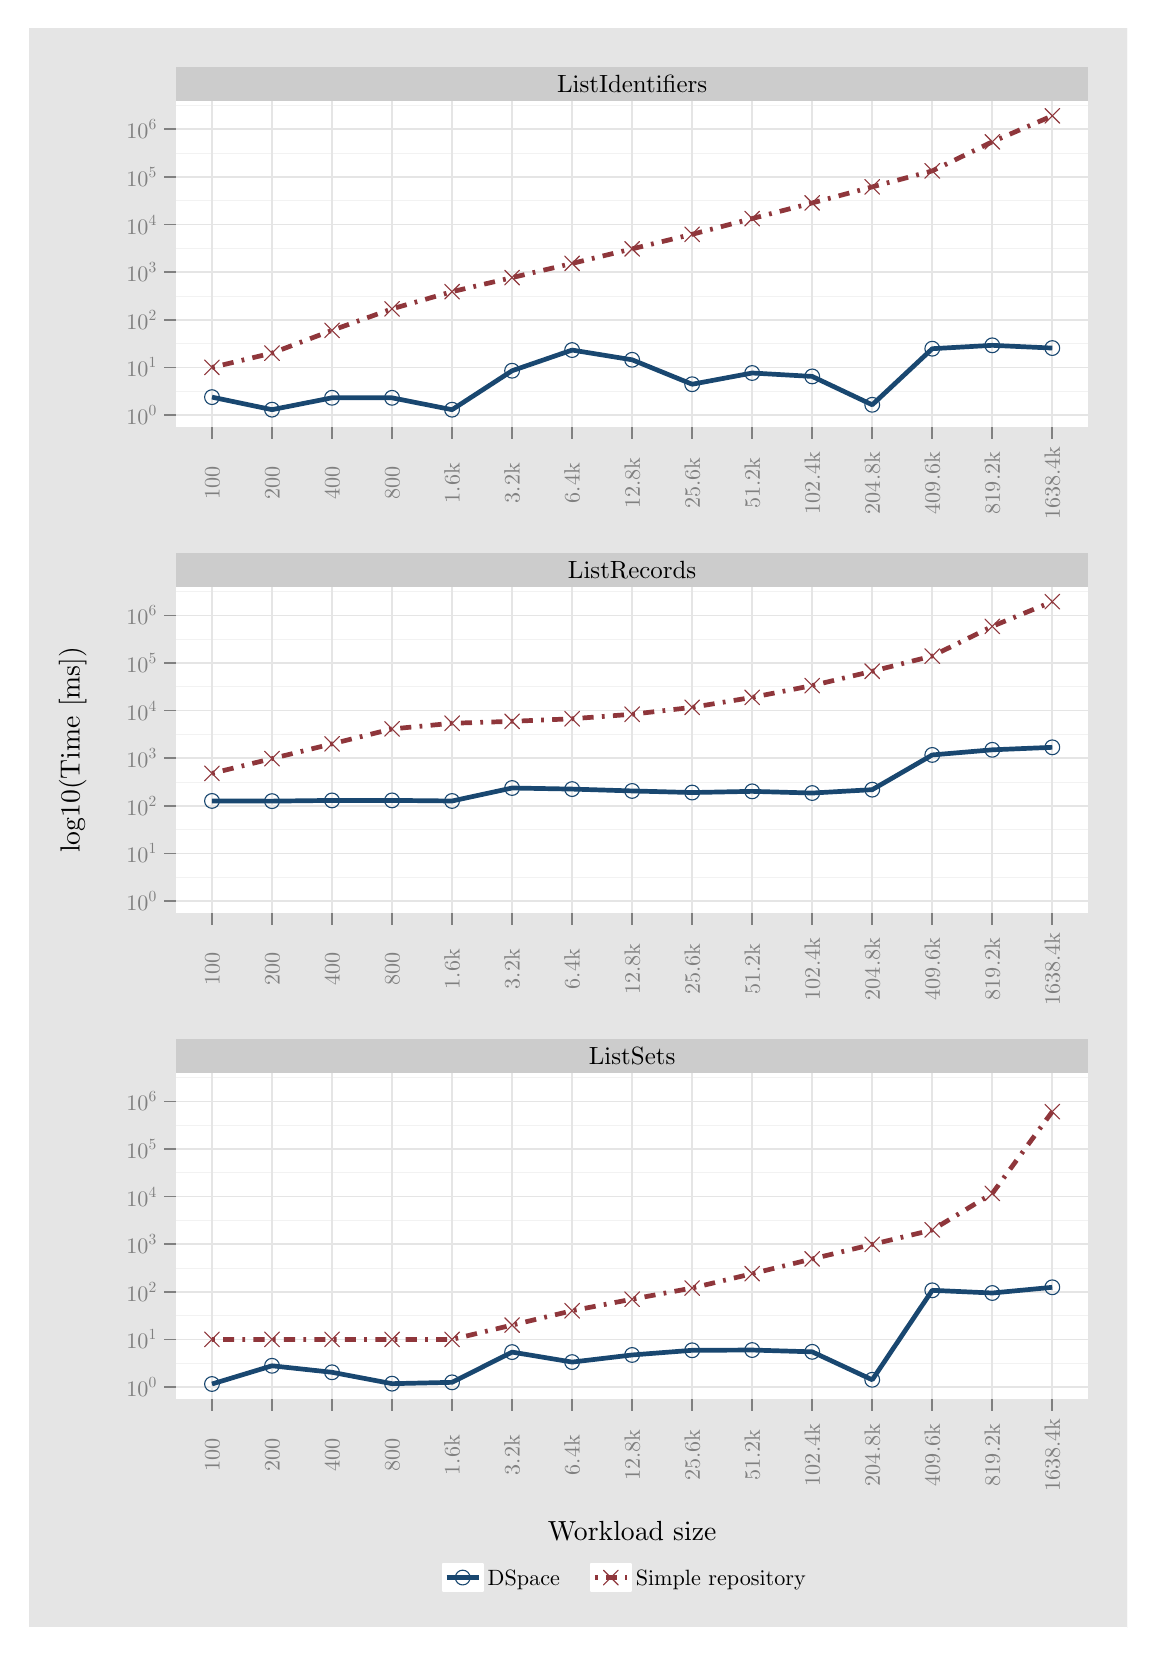
\begin{tikzpicture}[x=1pt,y=1pt]
\definecolor[named]{fillColor}{rgb}{1.00,1.00,1.00}
\path[use as bounding box,fill=fillColor,fill opacity=0.00] (0,0) rectangle (397.48,578.16);
\begin{scope}
\path[clip] (  0.00,  0.00) rectangle (397.48,578.16);
\definecolor[named]{drawColor}{rgb}{1.00,1.00,1.00}
\definecolor[named]{fillColor}{rgb}{0.90,0.90,0.90}

\path[draw=drawColor,line width= 0.6pt,line join=round,line cap=round,fill=fillColor] (  0.00,  0.00) rectangle (397.48,578.16);
\end{scope}
\begin{scope}
\path[clip] ( 53.58,433.92) rectangle (383.26,551.71);
\definecolor[named]{fillColor}{rgb}{1.00,1.00,1.00}

\path[fill=fillColor] ( 53.58,433.92) rectangle (383.26,551.71);
\definecolor[named]{drawColor}{rgb}{0.95,0.95,0.95}

\path[draw=drawColor,line width= 0.3pt,line join=round] ( 53.58,446.78) --
	(383.26,446.78);

\path[draw=drawColor,line width= 0.3pt,line join=round] ( 53.58,463.99) --
	(383.26,463.99);

\path[draw=drawColor,line width= 0.3pt,line join=round] ( 53.58,481.19) --
	(383.26,481.19);

\path[draw=drawColor,line width= 0.3pt,line join=round] ( 53.58,498.40) --
	(383.26,498.40);

\path[draw=drawColor,line width= 0.3pt,line join=round] ( 53.58,515.61) --
	(383.26,515.61);

\path[draw=drawColor,line width= 0.3pt,line join=round] ( 53.58,532.81) --
	(383.26,532.81);

\path[draw=drawColor,line width= 0.3pt,line join=round] ( 53.58,550.02) --
	(383.26,550.02);
\definecolor[named]{drawColor}{rgb}{0.90,0.90,0.90}

\path[draw=drawColor,line width= 0.6pt,line join=round] ( 53.58,438.17) --
	(383.26,438.17);

\path[draw=drawColor,line width= 0.6pt,line join=round] ( 53.58,455.38) --
	(383.26,455.38);

\path[draw=drawColor,line width= 0.6pt,line join=round] ( 53.58,472.59) --
	(383.26,472.59);

\path[draw=drawColor,line width= 0.6pt,line join=round] ( 53.58,489.80) --
	(383.26,489.80);

\path[draw=drawColor,line width= 0.6pt,line join=round] ( 53.58,507.00) --
	(383.26,507.00);

\path[draw=drawColor,line width= 0.6pt,line join=round] ( 53.58,524.21) --
	(383.26,524.21);

\path[draw=drawColor,line width= 0.6pt,line join=round] ( 53.58,541.42) --
	(383.26,541.42);

\path[draw=drawColor,line width= 0.6pt,line join=round] ( 66.60,433.92) --
	( 66.60,551.71);

\path[draw=drawColor,line width= 0.6pt,line join=round] ( 88.29,433.92) --
	( 88.29,551.71);

\path[draw=drawColor,line width= 0.6pt,line join=round] (109.97,433.92) --
	(109.97,551.71);

\path[draw=drawColor,line width= 0.6pt,line join=round] (131.66,433.92) --
	(131.66,551.71);

\path[draw=drawColor,line width= 0.6pt,line join=round] (153.35,433.92) --
	(153.35,551.71);

\path[draw=drawColor,line width= 0.6pt,line join=round] (175.04,433.92) --
	(175.04,551.71);

\path[draw=drawColor,line width= 0.6pt,line join=round] (196.73,433.92) --
	(196.73,551.71);

\path[draw=drawColor,line width= 0.6pt,line join=round] (218.42,433.92) --
	(218.42,551.71);

\path[draw=drawColor,line width= 0.6pt,line join=round] (240.11,433.92) --
	(240.11,551.71);

\path[draw=drawColor,line width= 0.6pt,line join=round] (261.80,433.92) --
	(261.80,551.71);

\path[draw=drawColor,line width= 0.6pt,line join=round] (283.49,433.92) --
	(283.49,551.71);

\path[draw=drawColor,line width= 0.6pt,line join=round] (305.18,433.92) --
	(305.18,551.71);

\path[draw=drawColor,line width= 0.6pt,line join=round] (326.87,433.92) --
	(326.87,551.71);

\path[draw=drawColor,line width= 0.6pt,line join=round] (348.56,433.92) --
	(348.56,551.71);

\path[draw=drawColor,line width= 0.6pt,line join=round] (370.25,433.92) --
	(370.25,551.71);
\definecolor[named]{drawColor}{rgb}{0.10,0.28,0.44}

\path[draw=drawColor,line width= 1.7pt,line join=round] ( 66.60,444.65) --
	( 88.29,440.12) --
	(109.97,444.41) --
	(131.66,444.40) --
	(153.35,440.11) --
	(175.04,454.19) --
	(196.73,461.66) --
	(218.42,458.14) --
	(240.11,449.31) --
	(261.80,453.37) --
	(283.49,452.13) --
	(305.18,441.88) --
	(326.87,462.15) --
	(348.56,463.37) --
	(370.25,462.38);
\definecolor[named]{drawColor}{rgb}{0.56,0.21,0.23}

\path[draw=drawColor,line width= 1.7pt,dash pattern=on 1pt off 3pt on 4pt off 3pt ,line join=round] ( 66.60,455.38) --
	( 88.29,460.56) --
	(109.97,468.77) --
	(131.66,476.55) --
	(153.35,482.76) --
	(175.04,487.84) --
	(196.73,492.97) --
	(218.42,498.23) --
	(240.11,503.49) --
	(261.80,509.18) --
	(283.49,514.82) --
	(305.18,520.62) --
	(326.87,526.39) --
	(348.56,536.92) --
	(370.25,546.30);
\definecolor[named]{drawColor}{rgb}{0.10,0.28,0.44}

\path[draw=drawColor,line width= 0.4pt,line join=round,line cap=round] ( 66.60,444.65) circle (  2.67);

\path[draw=drawColor,line width= 0.4pt,line join=round,line cap=round] ( 88.29,440.12) circle (  2.67);

\path[draw=drawColor,line width= 0.4pt,line join=round,line cap=round] (109.97,444.41) circle (  2.67);

\path[draw=drawColor,line width= 0.4pt,line join=round,line cap=round] (131.66,444.40) circle (  2.67);

\path[draw=drawColor,line width= 0.4pt,line join=round,line cap=round] (153.35,440.11) circle (  2.67);

\path[draw=drawColor,line width= 0.4pt,line join=round,line cap=round] (175.04,454.19) circle (  2.67);

\path[draw=drawColor,line width= 0.4pt,line join=round,line cap=round] (196.73,461.66) circle (  2.67);

\path[draw=drawColor,line width= 0.4pt,line join=round,line cap=round] (218.42,458.14) circle (  2.67);

\path[draw=drawColor,line width= 0.4pt,line join=round,line cap=round] (240.11,449.31) circle (  2.67);

\path[draw=drawColor,line width= 0.4pt,line join=round,line cap=round] (261.80,453.37) circle (  2.67);

\path[draw=drawColor,line width= 0.4pt,line join=round,line cap=round] (283.49,452.13) circle (  2.67);

\path[draw=drawColor,line width= 0.4pt,line join=round,line cap=round] (305.18,441.88) circle (  2.67);

\path[draw=drawColor,line width= 0.4pt,line join=round,line cap=round] (326.87,462.15) circle (  2.67);

\path[draw=drawColor,line width= 0.4pt,line join=round,line cap=round] (348.56,463.37) circle (  2.67);

\path[draw=drawColor,line width= 0.4pt,line join=round,line cap=round] (370.25,462.38) circle (  2.67);
\definecolor[named]{drawColor}{rgb}{0.56,0.21,0.23}

\path[draw=drawColor,line width= 0.4pt,line join=round,line cap=round,fill=fillColor] ( 63.93,452.71) -- ( 69.26,458.05);

\path[draw=drawColor,line width= 0.4pt,line join=round,line cap=round,fill=fillColor] ( 63.93,458.05) -- ( 69.26,452.71);

\path[draw=drawColor,line width= 0.4pt,line join=round,line cap=round,fill=fillColor] ( 85.62,457.89) -- ( 90.95,463.23);

\path[draw=drawColor,line width= 0.4pt,line join=round,line cap=round,fill=fillColor] ( 85.62,463.23) -- ( 90.95,457.89);

\path[draw=drawColor,line width= 0.4pt,line join=round,line cap=round,fill=fillColor] (107.31,466.10) -- (112.64,471.44);

\path[draw=drawColor,line width= 0.4pt,line join=round,line cap=round,fill=fillColor] (107.31,471.44) -- (112.64,466.10);

\path[draw=drawColor,line width= 0.4pt,line join=round,line cap=round,fill=fillColor] (129.00,473.89) -- (134.33,479.22);

\path[draw=drawColor,line width= 0.4pt,line join=round,line cap=round,fill=fillColor] (129.00,479.22) -- (134.33,473.89);

\path[draw=drawColor,line width= 0.4pt,line join=round,line cap=round,fill=fillColor] (150.69,480.09) -- (156.02,485.43);

\path[draw=drawColor,line width= 0.4pt,line join=round,line cap=round,fill=fillColor] (150.69,485.43) -- (156.02,480.09);

\path[draw=drawColor,line width= 0.4pt,line join=round,line cap=round,fill=fillColor] (172.37,485.18) -- (177.71,490.51);

\path[draw=drawColor,line width= 0.4pt,line join=round,line cap=round,fill=fillColor] (172.37,490.51) -- (177.71,485.18);

\path[draw=drawColor,line width= 0.4pt,line join=round,line cap=round,fill=fillColor] (194.06,490.31) -- (199.40,495.64);

\path[draw=drawColor,line width= 0.4pt,line join=round,line cap=round,fill=fillColor] (194.06,495.64) -- (199.40,490.31);

\path[draw=drawColor,line width= 0.4pt,line join=round,line cap=round,fill=fillColor] (215.75,495.56) -- (221.09,500.89);

\path[draw=drawColor,line width= 0.4pt,line join=round,line cap=round,fill=fillColor] (215.75,500.89) -- (221.09,495.56);

\path[draw=drawColor,line width= 0.4pt,line join=round,line cap=round,fill=fillColor] (237.44,500.82) -- (242.78,506.16);

\path[draw=drawColor,line width= 0.4pt,line join=round,line cap=round,fill=fillColor] (237.44,506.16) -- (242.78,500.82);

\path[draw=drawColor,line width= 0.4pt,line join=round,line cap=round,fill=fillColor] (259.13,506.51) -- (264.47,511.85);

\path[draw=drawColor,line width= 0.4pt,line join=round,line cap=round,fill=fillColor] (259.13,511.85) -- (264.47,506.51);

\path[draw=drawColor,line width= 0.4pt,line join=round,line cap=round,fill=fillColor] (280.82,512.15) -- (286.16,517.49);

\path[draw=drawColor,line width= 0.4pt,line join=round,line cap=round,fill=fillColor] (280.82,517.49) -- (286.16,512.15);

\path[draw=drawColor,line width= 0.4pt,line join=round,line cap=round,fill=fillColor] (302.51,517.95) -- (307.84,523.29);

\path[draw=drawColor,line width= 0.4pt,line join=round,line cap=round,fill=fillColor] (302.51,523.29) -- (307.84,517.95);

\path[draw=drawColor,line width= 0.4pt,line join=round,line cap=round,fill=fillColor] (324.20,523.73) -- (329.53,529.06);

\path[draw=drawColor,line width= 0.4pt,line join=round,line cap=round,fill=fillColor] (324.20,529.06) -- (329.53,523.73);

\path[draw=drawColor,line width= 0.4pt,line join=round,line cap=round,fill=fillColor] (345.89,534.26) -- (351.22,539.59);

\path[draw=drawColor,line width= 0.4pt,line join=round,line cap=round,fill=fillColor] (345.89,539.59) -- (351.22,534.26);

\path[draw=drawColor,line width= 0.4pt,line join=round,line cap=round,fill=fillColor] (367.58,543.64) -- (372.91,548.97);

\path[draw=drawColor,line width= 0.4pt,line join=round,line cap=round,fill=fillColor] (367.58,548.97) -- (372.91,543.64);
\end{scope}
\begin{scope}
\path[clip] ( 53.58,258.30) rectangle (383.26,376.10);
\definecolor[named]{fillColor}{rgb}{1.00,1.00,1.00}

\path[fill=fillColor] ( 53.58,258.30) rectangle (383.26,376.10);
\definecolor[named]{drawColor}{rgb}{0.95,0.95,0.95}

\path[draw=drawColor,line width= 0.3pt,line join=round] ( 53.58,271.17) --
	(383.26,271.17);

\path[draw=drawColor,line width= 0.3pt,line join=round] ( 53.58,288.37) --
	(383.26,288.37);

\path[draw=drawColor,line width= 0.3pt,line join=round] ( 53.58,305.58) --
	(383.26,305.58);

\path[draw=drawColor,line width= 0.3pt,line join=round] ( 53.58,322.79) --
	(383.26,322.79);

\path[draw=drawColor,line width= 0.3pt,line join=round] ( 53.58,339.99) --
	(383.26,339.99);

\path[draw=drawColor,line width= 0.3pt,line join=round] ( 53.58,357.20) --
	(383.26,357.20);

\path[draw=drawColor,line width= 0.3pt,line join=round] ( 53.58,374.41) --
	(383.26,374.41);
\definecolor[named]{drawColor}{rgb}{0.90,0.90,0.90}

\path[draw=drawColor,line width= 0.6pt,line join=round] ( 53.58,262.56) --
	(383.26,262.56);

\path[draw=drawColor,line width= 0.6pt,line join=round] ( 53.58,279.77) --
	(383.26,279.77);

\path[draw=drawColor,line width= 0.6pt,line join=round] ( 53.58,296.98) --
	(383.26,296.98);

\path[draw=drawColor,line width= 0.6pt,line join=round] ( 53.58,314.18) --
	(383.26,314.18);

\path[draw=drawColor,line width= 0.6pt,line join=round] ( 53.58,331.39) --
	(383.26,331.39);

\path[draw=drawColor,line width= 0.6pt,line join=round] ( 53.58,348.60) --
	(383.26,348.60);

\path[draw=drawColor,line width= 0.6pt,line join=round] ( 53.58,365.80) --
	(383.26,365.80);

\path[draw=drawColor,line width= 0.6pt,line join=round] ( 66.60,258.30) --
	( 66.60,376.10);

\path[draw=drawColor,line width= 0.6pt,line join=round] ( 88.29,258.30) --
	( 88.29,376.10);

\path[draw=drawColor,line width= 0.6pt,line join=round] (109.97,258.30) --
	(109.97,376.10);

\path[draw=drawColor,line width= 0.6pt,line join=round] (131.66,258.30) --
	(131.66,376.10);

\path[draw=drawColor,line width= 0.6pt,line join=round] (153.35,258.30) --
	(153.35,376.10);

\path[draw=drawColor,line width= 0.6pt,line join=round] (175.04,258.30) --
	(175.04,376.10);

\path[draw=drawColor,line width= 0.6pt,line join=round] (196.73,258.30) --
	(196.73,376.10);

\path[draw=drawColor,line width= 0.6pt,line join=round] (218.42,258.30) --
	(218.42,376.10);

\path[draw=drawColor,line width= 0.6pt,line join=round] (240.11,258.30) --
	(240.11,376.10);

\path[draw=drawColor,line width= 0.6pt,line join=round] (261.80,258.30) --
	(261.80,376.10);

\path[draw=drawColor,line width= 0.6pt,line join=round] (283.49,258.30) --
	(283.49,376.10);

\path[draw=drawColor,line width= 0.6pt,line join=round] (305.18,258.30) --
	(305.18,376.10);

\path[draw=drawColor,line width= 0.6pt,line join=round] (326.87,258.30) --
	(326.87,376.10);

\path[draw=drawColor,line width= 0.6pt,line join=round] (348.56,258.30) --
	(348.56,376.10);

\path[draw=drawColor,line width= 0.6pt,line join=round] (370.25,258.30) --
	(370.25,376.10);
\definecolor[named]{drawColor}{rgb}{0.10,0.28,0.44}

\path[draw=drawColor,line width= 1.7pt,line join=round] ( 66.60,298.74) --
	( 88.29,298.67) --
	(109.97,298.92) --
	(131.66,298.93) --
	(153.35,298.72) --
	(175.04,303.41) --
	(196.73,303.02) --
	(218.42,302.35) --
	(240.11,301.77) --
	(261.80,302.20) --
	(283.49,301.59) --
	(305.18,302.81) --
	(326.87,315.36) --
	(348.56,317.21) --
	(370.25,318.11);
\definecolor[named]{drawColor}{rgb}{0.56,0.21,0.23}

\path[draw=drawColor,line width= 1.7pt,dash pattern=on 1pt off 3pt on 4pt off 3pt ,line join=round] ( 66.60,308.70) --
	( 88.29,314.03) --
	(109.97,319.36) --
	(131.66,324.76) --
	(153.35,326.80) --
	(175.04,327.50) --
	(196.73,328.43) --
	(218.42,330.06) --
	(240.11,332.55) --
	(261.80,336.15) --
	(283.49,340.42) --
	(305.18,345.60) --
	(326.87,351.10) --
	(348.56,361.82) --
	(370.25,370.75);
\definecolor[named]{drawColor}{rgb}{0.10,0.28,0.44}

\path[draw=drawColor,line width= 0.4pt,line join=round,line cap=round] ( 66.60,298.74) circle (  2.67);

\path[draw=drawColor,line width= 0.4pt,line join=round,line cap=round] ( 88.29,298.67) circle (  2.67);

\path[draw=drawColor,line width= 0.4pt,line join=round,line cap=round] (109.97,298.92) circle (  2.67);

\path[draw=drawColor,line width= 0.4pt,line join=round,line cap=round] (131.66,298.93) circle (  2.67);

\path[draw=drawColor,line width= 0.4pt,line join=round,line cap=round] (153.35,298.72) circle (  2.67);

\path[draw=drawColor,line width= 0.4pt,line join=round,line cap=round] (175.04,303.41) circle (  2.67);

\path[draw=drawColor,line width= 0.4pt,line join=round,line cap=round] (196.73,303.02) circle (  2.67);

\path[draw=drawColor,line width= 0.4pt,line join=round,line cap=round] (218.42,302.35) circle (  2.67);

\path[draw=drawColor,line width= 0.4pt,line join=round,line cap=round] (240.11,301.77) circle (  2.67);

\path[draw=drawColor,line width= 0.4pt,line join=round,line cap=round] (261.80,302.20) circle (  2.67);

\path[draw=drawColor,line width= 0.4pt,line join=round,line cap=round] (283.49,301.59) circle (  2.67);

\path[draw=drawColor,line width= 0.4pt,line join=round,line cap=round] (305.18,302.81) circle (  2.67);

\path[draw=drawColor,line width= 0.4pt,line join=round,line cap=round] (326.87,315.36) circle (  2.67);

\path[draw=drawColor,line width= 0.4pt,line join=round,line cap=round] (348.56,317.21) circle (  2.67);

\path[draw=drawColor,line width= 0.4pt,line join=round,line cap=round] (370.25,318.11) circle (  2.67);
\definecolor[named]{drawColor}{rgb}{0.56,0.21,0.23}

\path[draw=drawColor,line width= 0.4pt,line join=round,line cap=round,fill=fillColor] ( 63.93,306.03) -- ( 69.26,311.37);

\path[draw=drawColor,line width= 0.4pt,line join=round,line cap=round,fill=fillColor] ( 63.93,311.37) -- ( 69.26,306.03);

\path[draw=drawColor,line width= 0.4pt,line join=round,line cap=round,fill=fillColor] ( 85.62,311.36) -- ( 90.95,316.70);

\path[draw=drawColor,line width= 0.4pt,line join=round,line cap=round,fill=fillColor] ( 85.62,316.70) -- ( 90.95,311.36);

\path[draw=drawColor,line width= 0.4pt,line join=round,line cap=round,fill=fillColor] (107.31,316.70) -- (112.64,322.03);

\path[draw=drawColor,line width= 0.4pt,line join=round,line cap=round,fill=fillColor] (107.31,322.03) -- (112.64,316.70);

\path[draw=drawColor,line width= 0.4pt,line join=round,line cap=round,fill=fillColor] (129.00,322.10) -- (134.33,327.43);

\path[draw=drawColor,line width= 0.4pt,line join=round,line cap=round,fill=fillColor] (129.00,327.43) -- (134.33,322.10);

\path[draw=drawColor,line width= 0.4pt,line join=round,line cap=round,fill=fillColor] (150.69,324.13) -- (156.02,329.47);

\path[draw=drawColor,line width= 0.4pt,line join=round,line cap=round,fill=fillColor] (150.69,329.47) -- (156.02,324.13);

\path[draw=drawColor,line width= 0.4pt,line join=round,line cap=round,fill=fillColor] (172.37,324.83) -- (177.71,330.17);

\path[draw=drawColor,line width= 0.4pt,line join=round,line cap=round,fill=fillColor] (172.37,330.17) -- (177.71,324.83);

\path[draw=drawColor,line width= 0.4pt,line join=round,line cap=round,fill=fillColor] (194.06,325.76) -- (199.40,331.10);

\path[draw=drawColor,line width= 0.4pt,line join=round,line cap=round,fill=fillColor] (194.06,331.10) -- (199.40,325.76);

\path[draw=drawColor,line width= 0.4pt,line join=round,line cap=round,fill=fillColor] (215.75,327.39) -- (221.09,332.73);

\path[draw=drawColor,line width= 0.4pt,line join=round,line cap=round,fill=fillColor] (215.75,332.73) -- (221.09,327.39);

\path[draw=drawColor,line width= 0.4pt,line join=round,line cap=round,fill=fillColor] (237.44,329.88) -- (242.78,335.22);

\path[draw=drawColor,line width= 0.4pt,line join=round,line cap=round,fill=fillColor] (237.44,335.22) -- (242.78,329.88);

\path[draw=drawColor,line width= 0.4pt,line join=round,line cap=round,fill=fillColor] (259.13,333.48) -- (264.47,338.81);

\path[draw=drawColor,line width= 0.4pt,line join=round,line cap=round,fill=fillColor] (259.13,338.81) -- (264.47,333.48);

\path[draw=drawColor,line width= 0.4pt,line join=round,line cap=round,fill=fillColor] (280.82,337.75) -- (286.16,343.08);

\path[draw=drawColor,line width= 0.4pt,line join=round,line cap=round,fill=fillColor] (280.82,343.08) -- (286.16,337.75);

\path[draw=drawColor,line width= 0.4pt,line join=round,line cap=round,fill=fillColor] (302.51,342.93) -- (307.84,348.27);

\path[draw=drawColor,line width= 0.4pt,line join=round,line cap=round,fill=fillColor] (302.51,348.27) -- (307.84,342.93);

\path[draw=drawColor,line width= 0.4pt,line join=round,line cap=round,fill=fillColor] (324.20,348.43) -- (329.53,353.76);

\path[draw=drawColor,line width= 0.4pt,line join=round,line cap=round,fill=fillColor] (324.20,353.76) -- (329.53,348.43);

\path[draw=drawColor,line width= 0.4pt,line join=round,line cap=round,fill=fillColor] (345.89,359.15) -- (351.22,364.48);

\path[draw=drawColor,line width= 0.4pt,line join=round,line cap=round,fill=fillColor] (345.89,364.48) -- (351.22,359.15);

\path[draw=drawColor,line width= 0.4pt,line join=round,line cap=round,fill=fillColor] (367.58,368.08) -- (372.91,373.41);

\path[draw=drawColor,line width= 0.4pt,line join=round,line cap=round,fill=fillColor] (367.58,373.41) -- (372.91,368.08);
\end{scope}
\begin{scope}
\path[clip] ( 53.58, 82.69) rectangle (383.26,200.49);
\definecolor[named]{fillColor}{rgb}{1.00,1.00,1.00}

\path[fill=fillColor] ( 53.58, 82.69) rectangle (383.26,200.49);
\definecolor[named]{drawColor}{rgb}{0.95,0.95,0.95}

\path[draw=drawColor,line width= 0.3pt,line join=round] ( 53.58, 95.55) --
	(383.26, 95.55);

\path[draw=drawColor,line width= 0.3pt,line join=round] ( 53.58,112.76) --
	(383.26,112.76);

\path[draw=drawColor,line width= 0.3pt,line join=round] ( 53.58,129.97) --
	(383.26,129.97);

\path[draw=drawColor,line width= 0.3pt,line join=round] ( 53.58,147.17) --
	(383.26,147.17);

\path[draw=drawColor,line width= 0.3pt,line join=round] ( 53.58,164.38) --
	(383.26,164.38);

\path[draw=drawColor,line width= 0.3pt,line join=round] ( 53.58,181.59) --
	(383.26,181.59);

\path[draw=drawColor,line width= 0.3pt,line join=round] ( 53.58,198.79) --
	(383.26,198.79);
\definecolor[named]{drawColor}{rgb}{0.90,0.90,0.90}

\path[draw=drawColor,line width= 0.6pt,line join=round] ( 53.58, 86.95) --
	(383.26, 86.95);

\path[draw=drawColor,line width= 0.6pt,line join=round] ( 53.58,104.16) --
	(383.26,104.16);

\path[draw=drawColor,line width= 0.6pt,line join=round] ( 53.58,121.36) --
	(383.26,121.36);

\path[draw=drawColor,line width= 0.6pt,line join=round] ( 53.58,138.57) --
	(383.26,138.57);

\path[draw=drawColor,line width= 0.6pt,line join=round] ( 53.58,155.78) --
	(383.26,155.78);

\path[draw=drawColor,line width= 0.6pt,line join=round] ( 53.58,172.98) --
	(383.26,172.98);

\path[draw=drawColor,line width= 0.6pt,line join=round] ( 53.58,190.19) --
	(383.26,190.19);

\path[draw=drawColor,line width= 0.6pt,line join=round] ( 66.60, 82.69) --
	( 66.60,200.49);

\path[draw=drawColor,line width= 0.6pt,line join=round] ( 88.29, 82.69) --
	( 88.29,200.49);

\path[draw=drawColor,line width= 0.6pt,line join=round] (109.97, 82.69) --
	(109.97,200.49);

\path[draw=drawColor,line width= 0.6pt,line join=round] (131.66, 82.69) --
	(131.66,200.49);

\path[draw=drawColor,line width= 0.6pt,line join=round] (153.35, 82.69) --
	(153.35,200.49);

\path[draw=drawColor,line width= 0.6pt,line join=round] (175.04, 82.69) --
	(175.04,200.49);

\path[draw=drawColor,line width= 0.6pt,line join=round] (196.73, 82.69) --
	(196.73,200.49);

\path[draw=drawColor,line width= 0.6pt,line join=round] (218.42, 82.69) --
	(218.42,200.49);

\path[draw=drawColor,line width= 0.6pt,line join=round] (240.11, 82.69) --
	(240.11,200.49);

\path[draw=drawColor,line width= 0.6pt,line join=round] (261.80, 82.69) --
	(261.80,200.49);

\path[draw=drawColor,line width= 0.6pt,line join=round] (283.49, 82.69) --
	(283.49,200.49);

\path[draw=drawColor,line width= 0.6pt,line join=round] (305.18, 82.69) --
	(305.18,200.49);

\path[draw=drawColor,line width= 0.6pt,line join=round] (326.87, 82.69) --
	(326.87,200.49);

\path[draw=drawColor,line width= 0.6pt,line join=round] (348.56, 82.69) --
	(348.56,200.49);

\path[draw=drawColor,line width= 0.6pt,line join=round] (370.25, 82.69) --
	(370.25,200.49);
\definecolor[named]{drawColor}{rgb}{0.10,0.28,0.44}

\path[draw=drawColor,line width= 1.7pt,line join=round] ( 66.60, 88.05) --
	( 88.29, 94.63) --
	(109.97, 92.28) --
	(131.66, 88.17) --
	(153.35, 88.65) --
	(175.04, 99.58) --
	(196.73, 95.97) --
	(218.42, 98.54) --
	(240.11,100.23) --
	(261.80,100.32) --
	(283.49, 99.67) --
	(305.18, 89.57) --
	(326.87,121.90) --
	(348.56,120.93) --
	(370.25,122.99);
\definecolor[named]{drawColor}{rgb}{0.56,0.21,0.23}

\path[draw=drawColor,line width= 1.7pt,dash pattern=on 1pt off 3pt on 4pt off 3pt ,line join=round] ( 66.60,104.16) --
	( 88.29,104.16) --
	(109.97,104.16) --
	(131.66,104.16) --
	(153.35,104.16) --
	(175.04,109.34) --
	(196.73,114.52) --
	(218.42,118.70) --
	(240.11,122.73) --
	(261.80,127.91) --
	(283.49,133.24) --
	(305.18,138.49) --
	(326.87,143.71) --
	(348.56,156.89) --
	(370.25,186.49);
\definecolor[named]{drawColor}{rgb}{0.10,0.28,0.44}

\path[draw=drawColor,line width= 0.4pt,line join=round,line cap=round] ( 66.60, 88.05) circle (  2.67);

\path[draw=drawColor,line width= 0.4pt,line join=round,line cap=round] ( 88.29, 94.63) circle (  2.67);

\path[draw=drawColor,line width= 0.4pt,line join=round,line cap=round] (109.97, 92.28) circle (  2.67);

\path[draw=drawColor,line width= 0.4pt,line join=round,line cap=round] (131.66, 88.17) circle (  2.67);

\path[draw=drawColor,line width= 0.4pt,line join=round,line cap=round] (153.35, 88.65) circle (  2.67);

\path[draw=drawColor,line width= 0.4pt,line join=round,line cap=round] (175.04, 99.58) circle (  2.67);

\path[draw=drawColor,line width= 0.4pt,line join=round,line cap=round] (196.73, 95.97) circle (  2.67);

\path[draw=drawColor,line width= 0.4pt,line join=round,line cap=round] (218.42, 98.54) circle (  2.67);

\path[draw=drawColor,line width= 0.4pt,line join=round,line cap=round] (240.11,100.23) circle (  2.67);

\path[draw=drawColor,line width= 0.4pt,line join=round,line cap=round] (261.80,100.32) circle (  2.67);

\path[draw=drawColor,line width= 0.4pt,line join=round,line cap=round] (283.49, 99.67) circle (  2.67);

\path[draw=drawColor,line width= 0.4pt,line join=round,line cap=round] (305.18, 89.57) circle (  2.67);

\path[draw=drawColor,line width= 0.4pt,line join=round,line cap=round] (326.87,121.90) circle (  2.67);

\path[draw=drawColor,line width= 0.4pt,line join=round,line cap=round] (348.56,120.93) circle (  2.67);

\path[draw=drawColor,line width= 0.4pt,line join=round,line cap=round] (370.25,122.99) circle (  2.67);
\definecolor[named]{drawColor}{rgb}{0.56,0.21,0.23}

\path[draw=drawColor,line width= 0.4pt,line join=round,line cap=round,fill=fillColor] ( 63.93,101.49) -- ( 69.26,106.82);

\path[draw=drawColor,line width= 0.4pt,line join=round,line cap=round,fill=fillColor] ( 63.93,106.82) -- ( 69.26,101.49);

\path[draw=drawColor,line width= 0.4pt,line join=round,line cap=round,fill=fillColor] ( 85.62,101.49) -- ( 90.95,106.82);

\path[draw=drawColor,line width= 0.4pt,line join=round,line cap=round,fill=fillColor] ( 85.62,106.82) -- ( 90.95,101.49);

\path[draw=drawColor,line width= 0.4pt,line join=round,line cap=round,fill=fillColor] (107.31,101.49) -- (112.64,106.82);

\path[draw=drawColor,line width= 0.4pt,line join=round,line cap=round,fill=fillColor] (107.31,106.82) -- (112.64,101.49);

\path[draw=drawColor,line width= 0.4pt,line join=round,line cap=round,fill=fillColor] (129.00,101.49) -- (134.33,106.82);

\path[draw=drawColor,line width= 0.4pt,line join=round,line cap=round,fill=fillColor] (129.00,106.82) -- (134.33,101.49);

\path[draw=drawColor,line width= 0.4pt,line join=round,line cap=round,fill=fillColor] (150.69,101.49) -- (156.02,106.82);

\path[draw=drawColor,line width= 0.4pt,line join=round,line cap=round,fill=fillColor] (150.69,106.82) -- (156.02,101.49);

\path[draw=drawColor,line width= 0.4pt,line join=round,line cap=round,fill=fillColor] (172.37,106.67) -- (177.71,112.00);

\path[draw=drawColor,line width= 0.4pt,line join=round,line cap=round,fill=fillColor] (172.37,112.00) -- (177.71,106.67);

\path[draw=drawColor,line width= 0.4pt,line join=round,line cap=round,fill=fillColor] (194.06,111.85) -- (199.40,117.18);

\path[draw=drawColor,line width= 0.4pt,line join=round,line cap=round,fill=fillColor] (194.06,117.18) -- (199.40,111.85);

\path[draw=drawColor,line width= 0.4pt,line join=round,line cap=round,fill=fillColor] (215.75,116.03) -- (221.09,121.37);

\path[draw=drawColor,line width= 0.4pt,line join=round,line cap=round,fill=fillColor] (215.75,121.37) -- (221.09,116.03);

\path[draw=drawColor,line width= 0.4pt,line join=round,line cap=round,fill=fillColor] (237.44,120.06) -- (242.78,125.39);

\path[draw=drawColor,line width= 0.4pt,line join=round,line cap=round,fill=fillColor] (237.44,125.39) -- (242.78,120.06);

\path[draw=drawColor,line width= 0.4pt,line join=round,line cap=round,fill=fillColor] (259.13,125.24) -- (264.47,130.57);

\path[draw=drawColor,line width= 0.4pt,line join=round,line cap=round,fill=fillColor] (259.13,130.57) -- (264.47,125.24);

\path[draw=drawColor,line width= 0.4pt,line join=round,line cap=round,fill=fillColor] (280.82,130.57) -- (286.16,135.91);

\path[draw=drawColor,line width= 0.4pt,line join=round,line cap=round,fill=fillColor] (280.82,135.91) -- (286.16,130.57);

\path[draw=drawColor,line width= 0.4pt,line join=round,line cap=round,fill=fillColor] (302.51,135.83) -- (307.84,141.16);

\path[draw=drawColor,line width= 0.4pt,line join=round,line cap=round,fill=fillColor] (302.51,141.16) -- (307.84,135.83);

\path[draw=drawColor,line width= 0.4pt,line join=round,line cap=round,fill=fillColor] (324.20,141.05) -- (329.53,146.38);

\path[draw=drawColor,line width= 0.4pt,line join=round,line cap=round,fill=fillColor] (324.20,146.38) -- (329.53,141.05);

\path[draw=drawColor,line width= 0.4pt,line join=round,line cap=round,fill=fillColor] (345.89,154.23) -- (351.22,159.56);

\path[draw=drawColor,line width= 0.4pt,line join=round,line cap=round,fill=fillColor] (345.89,159.56) -- (351.22,154.23);

\path[draw=drawColor,line width= 0.4pt,line join=round,line cap=round,fill=fillColor] (367.58,183.82) -- (372.91,189.15);

\path[draw=drawColor,line width= 0.4pt,line join=round,line cap=round,fill=fillColor] (367.58,189.15) -- (372.91,183.82);
\end{scope}
\begin{scope}
\path[clip] (  0.00,  0.00) rectangle (397.48,578.16);
\definecolor[named]{fillColor}{rgb}{0.80,0.80,0.80}

\path[fill=fillColor] ( 53.58,551.71) rectangle (383.26,563.93);
\definecolor[named]{drawColor}{rgb}{0.00,0.00,0.00}

\node[text=drawColor,anchor=base,inner sep=0pt, outer sep=0pt, scale=  0.90] at (218.42,554.72) {ListIdentifiers};
\end{scope}
\begin{scope}
\path[clip] (  0.00,  0.00) rectangle (397.48,578.16);
\definecolor[named]{fillColor}{rgb}{0.80,0.80,0.80}

\path[fill=fillColor] ( 53.58,376.10) rectangle (383.26,388.32);
\definecolor[named]{drawColor}{rgb}{0.00,0.00,0.00}

\node[text=drawColor,anchor=base,inner sep=0pt, outer sep=0pt, scale=  0.90] at (218.42,379.11) {ListRecords};
\end{scope}
\begin{scope}
\path[clip] (  0.00,  0.00) rectangle (397.48,578.16);
\definecolor[named]{fillColor}{rgb}{0.80,0.80,0.80}

\path[fill=fillColor] ( 53.58,200.49) rectangle (383.26,212.71);
\definecolor[named]{drawColor}{rgb}{0.00,0.00,0.00}

\node[text=drawColor,anchor=base,inner sep=0pt, outer sep=0pt, scale=  0.90] at (218.42,203.50) {ListSets};
\end{scope}
\begin{scope}
\path[clip] (  0.00,  0.00) rectangle (397.48,578.16);
\definecolor[named]{drawColor}{rgb}{0.50,0.50,0.50}

\node[text=drawColor,anchor=base west,inner sep=0pt, outer sep=0pt, scale=  0.80] at ( 35.67,434.74) {10};

\node[text=drawColor,anchor=base west,inner sep=0pt, outer sep=0pt, scale=  0.56] at ( 43.67,438.01) {0};

\node[text=drawColor,anchor=base west,inner sep=0pt, outer sep=0pt, scale=  0.80] at ( 35.67,451.95) {10};

\node[text=drawColor,anchor=base west,inner sep=0pt, outer sep=0pt, scale=  0.56] at ( 43.67,455.22) {1};

\node[text=drawColor,anchor=base west,inner sep=0pt, outer sep=0pt, scale=  0.80] at ( 35.67,469.16) {10};

\node[text=drawColor,anchor=base west,inner sep=0pt, outer sep=0pt, scale=  0.56] at ( 43.67,472.43) {2};

\node[text=drawColor,anchor=base west,inner sep=0pt, outer sep=0pt, scale=  0.80] at ( 35.67,486.36) {10};

\node[text=drawColor,anchor=base west,inner sep=0pt, outer sep=0pt, scale=  0.56] at ( 43.67,489.64) {3};

\node[text=drawColor,anchor=base west,inner sep=0pt, outer sep=0pt, scale=  0.80] at ( 35.67,503.57) {10};

\node[text=drawColor,anchor=base west,inner sep=0pt, outer sep=0pt, scale=  0.56] at ( 43.67,506.84) {4};

\node[text=drawColor,anchor=base west,inner sep=0pt, outer sep=0pt, scale=  0.80] at ( 35.67,520.78) {10};

\node[text=drawColor,anchor=base west,inner sep=0pt, outer sep=0pt, scale=  0.56] at ( 43.67,524.05) {5};

\node[text=drawColor,anchor=base west,inner sep=0pt, outer sep=0pt, scale=  0.80] at ( 35.67,537.99) {10};

\node[text=drawColor,anchor=base west,inner sep=0pt, outer sep=0pt, scale=  0.56] at ( 43.67,541.26) {6};
\end{scope}
\begin{scope}
\path[clip] (  0.00,  0.00) rectangle (397.48,578.16);
\definecolor[named]{drawColor}{rgb}{0.50,0.50,0.50}

\path[draw=drawColor,line width= 0.6pt,line join=round] ( 49.31,438.17) --
	( 53.58,438.17);

\path[draw=drawColor,line width= 0.6pt,line join=round] ( 49.31,455.38) --
	( 53.58,455.38);

\path[draw=drawColor,line width= 0.6pt,line join=round] ( 49.31,472.59) --
	( 53.58,472.59);

\path[draw=drawColor,line width= 0.6pt,line join=round] ( 49.31,489.80) --
	( 53.58,489.80);

\path[draw=drawColor,line width= 0.6pt,line join=round] ( 49.31,507.00) --
	( 53.58,507.00);

\path[draw=drawColor,line width= 0.6pt,line join=round] ( 49.31,524.21) --
	( 53.58,524.21);

\path[draw=drawColor,line width= 0.6pt,line join=round] ( 49.31,541.42) --
	( 53.58,541.42);
\end{scope}
\begin{scope}
\path[clip] (  0.00,  0.00) rectangle (397.48,578.16);
\definecolor[named]{drawColor}{rgb}{0.50,0.50,0.50}

\node[text=drawColor,anchor=base west,inner sep=0pt, outer sep=0pt, scale=  0.80] at ( 35.67,259.13) {10};

\node[text=drawColor,anchor=base west,inner sep=0pt, outer sep=0pt, scale=  0.56] at ( 43.67,262.40) {0};

\node[text=drawColor,anchor=base west,inner sep=0pt, outer sep=0pt, scale=  0.80] at ( 35.67,276.34) {10};

\node[text=drawColor,anchor=base west,inner sep=0pt, outer sep=0pt, scale=  0.56] at ( 43.67,279.61) {1};

\node[text=drawColor,anchor=base west,inner sep=0pt, outer sep=0pt, scale=  0.80] at ( 35.67,293.54) {10};

\node[text=drawColor,anchor=base west,inner sep=0pt, outer sep=0pt, scale=  0.56] at ( 43.67,296.82) {2};

\node[text=drawColor,anchor=base west,inner sep=0pt, outer sep=0pt, scale=  0.80] at ( 35.67,310.75) {10};

\node[text=drawColor,anchor=base west,inner sep=0pt, outer sep=0pt, scale=  0.56] at ( 43.67,314.02) {3};

\node[text=drawColor,anchor=base west,inner sep=0pt, outer sep=0pt, scale=  0.80] at ( 35.67,327.96) {10};

\node[text=drawColor,anchor=base west,inner sep=0pt, outer sep=0pt, scale=  0.56] at ( 43.67,331.23) {4};

\node[text=drawColor,anchor=base west,inner sep=0pt, outer sep=0pt, scale=  0.80] at ( 35.67,345.17) {10};

\node[text=drawColor,anchor=base west,inner sep=0pt, outer sep=0pt, scale=  0.56] at ( 43.67,348.44) {5};

\node[text=drawColor,anchor=base west,inner sep=0pt, outer sep=0pt, scale=  0.80] at ( 35.67,362.37) {10};

\node[text=drawColor,anchor=base west,inner sep=0pt, outer sep=0pt, scale=  0.56] at ( 43.67,365.64) {6};
\end{scope}
\begin{scope}
\path[clip] (  0.00,  0.00) rectangle (397.48,578.16);
\definecolor[named]{drawColor}{rgb}{0.50,0.50,0.50}

\path[draw=drawColor,line width= 0.6pt,line join=round] ( 49.31,262.56) --
	( 53.58,262.56);

\path[draw=drawColor,line width= 0.6pt,line join=round] ( 49.31,279.77) --
	( 53.58,279.77);

\path[draw=drawColor,line width= 0.6pt,line join=round] ( 49.31,296.98) --
	( 53.58,296.98);

\path[draw=drawColor,line width= 0.6pt,line join=round] ( 49.31,314.18) --
	( 53.58,314.18);

\path[draw=drawColor,line width= 0.6pt,line join=round] ( 49.31,331.39) --
	( 53.58,331.39);

\path[draw=drawColor,line width= 0.6pt,line join=round] ( 49.31,348.60) --
	( 53.58,348.60);

\path[draw=drawColor,line width= 0.6pt,line join=round] ( 49.31,365.80) --
	( 53.58,365.80);
\end{scope}
\begin{scope}
\path[clip] (  0.00,  0.00) rectangle (397.48,578.16);
\definecolor[named]{drawColor}{rgb}{0.50,0.50,0.50}

\node[text=drawColor,anchor=base west,inner sep=0pt, outer sep=0pt, scale=  0.80] at ( 35.67, 83.52) {10};

\node[text=drawColor,anchor=base west,inner sep=0pt, outer sep=0pt, scale=  0.56] at ( 43.67, 86.79) {0};

\node[text=drawColor,anchor=base west,inner sep=0pt, outer sep=0pt, scale=  0.80] at ( 35.67,100.72) {10};

\node[text=drawColor,anchor=base west,inner sep=0pt, outer sep=0pt, scale=  0.56] at ( 43.67,104.00) {1};

\node[text=drawColor,anchor=base west,inner sep=0pt, outer sep=0pt, scale=  0.80] at ( 35.67,117.93) {10};

\node[text=drawColor,anchor=base west,inner sep=0pt, outer sep=0pt, scale=  0.56] at ( 43.67,121.20) {2};

\node[text=drawColor,anchor=base west,inner sep=0pt, outer sep=0pt, scale=  0.80] at ( 35.67,135.14) {10};

\node[text=drawColor,anchor=base west,inner sep=0pt, outer sep=0pt, scale=  0.56] at ( 43.67,138.41) {3};

\node[text=drawColor,anchor=base west,inner sep=0pt, outer sep=0pt, scale=  0.80] at ( 35.67,152.35) {10};

\node[text=drawColor,anchor=base west,inner sep=0pt, outer sep=0pt, scale=  0.56] at ( 43.67,155.62) {4};

\node[text=drawColor,anchor=base west,inner sep=0pt, outer sep=0pt, scale=  0.80] at ( 35.67,169.55) {10};

\node[text=drawColor,anchor=base west,inner sep=0pt, outer sep=0pt, scale=  0.56] at ( 43.67,172.82) {5};

\node[text=drawColor,anchor=base west,inner sep=0pt, outer sep=0pt, scale=  0.80] at ( 35.67,186.76) {10};

\node[text=drawColor,anchor=base west,inner sep=0pt, outer sep=0pt, scale=  0.56] at ( 43.67,190.03) {6};
\end{scope}
\begin{scope}
\path[clip] (  0.00,  0.00) rectangle (397.48,578.16);
\definecolor[named]{drawColor}{rgb}{0.50,0.50,0.50}

\path[draw=drawColor,line width= 0.6pt,line join=round] ( 49.31, 86.95) --
	( 53.58, 86.95);

\path[draw=drawColor,line width= 0.6pt,line join=round] ( 49.31,104.16) --
	( 53.58,104.16);

\path[draw=drawColor,line width= 0.6pt,line join=round] ( 49.31,121.36) --
	( 53.58,121.36);

\path[draw=drawColor,line width= 0.6pt,line join=round] ( 49.31,138.57) --
	( 53.58,138.57);

\path[draw=drawColor,line width= 0.6pt,line join=round] ( 49.31,155.78) --
	( 53.58,155.78);

\path[draw=drawColor,line width= 0.6pt,line join=round] ( 49.31,172.98) --
	( 53.58,172.98);

\path[draw=drawColor,line width= 0.6pt,line join=round] ( 49.31,190.19) --
	( 53.58,190.19);
\end{scope}
\begin{scope}
\path[clip] (  0.00,  0.00) rectangle (397.48,578.16);
\definecolor[named]{drawColor}{rgb}{0.50,0.50,0.50}

\path[draw=drawColor,line width= 0.6pt,line join=round] ( 66.60,429.65) --
	( 66.60,433.92);

\path[draw=drawColor,line width= 0.6pt,line join=round] ( 88.29,429.65) --
	( 88.29,433.92);

\path[draw=drawColor,line width= 0.6pt,line join=round] (109.97,429.65) --
	(109.97,433.92);

\path[draw=drawColor,line width= 0.6pt,line join=round] (131.66,429.65) --
	(131.66,433.92);

\path[draw=drawColor,line width= 0.6pt,line join=round] (153.35,429.65) --
	(153.35,433.92);

\path[draw=drawColor,line width= 0.6pt,line join=round] (175.04,429.65) --
	(175.04,433.92);

\path[draw=drawColor,line width= 0.6pt,line join=round] (196.73,429.65) --
	(196.73,433.92);

\path[draw=drawColor,line width= 0.6pt,line join=round] (218.42,429.65) --
	(218.42,433.92);

\path[draw=drawColor,line width= 0.6pt,line join=round] (240.11,429.65) --
	(240.11,433.92);

\path[draw=drawColor,line width= 0.6pt,line join=round] (261.80,429.65) --
	(261.80,433.92);

\path[draw=drawColor,line width= 0.6pt,line join=round] (283.49,429.65) --
	(283.49,433.92);

\path[draw=drawColor,line width= 0.6pt,line join=round] (305.18,429.65) --
	(305.18,433.92);

\path[draw=drawColor,line width= 0.6pt,line join=round] (326.87,429.65) --
	(326.87,433.92);

\path[draw=drawColor,line width= 0.6pt,line join=round] (348.56,429.65) --
	(348.56,433.92);

\path[draw=drawColor,line width= 0.6pt,line join=round] (370.25,429.65) --
	(370.25,433.92);
\end{scope}
\begin{scope}
\path[clip] (  0.00,  0.00) rectangle (397.48,578.16);
\definecolor[named]{drawColor}{rgb}{0.50,0.50,0.50}

\node[text=drawColor,rotate= 90.00,anchor=base,inner sep=0pt, outer sep=0pt, scale=  0.80] at ( 69.35,413.58) {100};

\node[text=drawColor,rotate= 90.00,anchor=base,inner sep=0pt, outer sep=0pt, scale=  0.80] at ( 91.04,413.58) {200};

\node[text=drawColor,rotate= 90.00,anchor=base,inner sep=0pt, outer sep=0pt, scale=  0.80] at (112.73,413.58) {400};

\node[text=drawColor,rotate= 90.00,anchor=base,inner sep=0pt, outer sep=0pt, scale=  0.80] at (134.42,413.58) {800};

\node[text=drawColor,rotate= 90.00,anchor=base,inner sep=0pt, outer sep=0pt, scale=  0.80] at (156.11,413.58) {1.6k};

\node[text=drawColor,rotate= 90.00,anchor=base,inner sep=0pt, outer sep=0pt, scale=  0.80] at (177.80,413.58) {3.2k};

\node[text=drawColor,rotate= 90.00,anchor=base,inner sep=0pt, outer sep=0pt, scale=  0.80] at (199.49,413.58) {6.4k};

\node[text=drawColor,rotate= 90.00,anchor=base,inner sep=0pt, outer sep=0pt, scale=  0.80] at (221.18,413.58) {12.8k};

\node[text=drawColor,rotate= 90.00,anchor=base,inner sep=0pt, outer sep=0pt, scale=  0.80] at (242.86,413.58) {25.6k};

\node[text=drawColor,rotate= 90.00,anchor=base,inner sep=0pt, outer sep=0pt, scale=  0.80] at (264.55,413.58) {51.2k};

\node[text=drawColor,rotate= 90.00,anchor=base,inner sep=0pt, outer sep=0pt, scale=  0.80] at (286.24,413.58) {102.4k};

\node[text=drawColor,rotate= 90.00,anchor=base,inner sep=0pt, outer sep=0pt, scale=  0.80] at (307.93,413.58) {204.8k};

\node[text=drawColor,rotate= 90.00,anchor=base,inner sep=0pt, outer sep=0pt, scale=  0.80] at (329.62,413.58) {409.6k};

\node[text=drawColor,rotate= 90.00,anchor=base,inner sep=0pt, outer sep=0pt, scale=  0.80] at (351.31,413.58) {819.2k};

\node[text=drawColor,rotate= 90.00,anchor=base,inner sep=0pt, outer sep=0pt, scale=  0.80] at (373.00,413.58) {1638.4k};
\end{scope}
\begin{scope}
\path[clip] (  0.00,  0.00) rectangle (397.48,578.16);
\definecolor[named]{drawColor}{rgb}{0.50,0.50,0.50}

\path[draw=drawColor,line width= 0.6pt,line join=round] ( 66.60,254.04) --
	( 66.60,258.30);

\path[draw=drawColor,line width= 0.6pt,line join=round] ( 88.29,254.04) --
	( 88.29,258.30);

\path[draw=drawColor,line width= 0.6pt,line join=round] (109.97,254.04) --
	(109.97,258.30);

\path[draw=drawColor,line width= 0.6pt,line join=round] (131.66,254.04) --
	(131.66,258.30);

\path[draw=drawColor,line width= 0.6pt,line join=round] (153.35,254.04) --
	(153.35,258.30);

\path[draw=drawColor,line width= 0.6pt,line join=round] (175.04,254.04) --
	(175.04,258.30);

\path[draw=drawColor,line width= 0.6pt,line join=round] (196.73,254.04) --
	(196.73,258.30);

\path[draw=drawColor,line width= 0.6pt,line join=round] (218.42,254.04) --
	(218.42,258.30);

\path[draw=drawColor,line width= 0.6pt,line join=round] (240.11,254.04) --
	(240.11,258.30);

\path[draw=drawColor,line width= 0.6pt,line join=round] (261.80,254.04) --
	(261.80,258.30);

\path[draw=drawColor,line width= 0.6pt,line join=round] (283.49,254.04) --
	(283.49,258.30);

\path[draw=drawColor,line width= 0.6pt,line join=round] (305.18,254.04) --
	(305.18,258.30);

\path[draw=drawColor,line width= 0.6pt,line join=round] (326.87,254.04) --
	(326.87,258.30);

\path[draw=drawColor,line width= 0.6pt,line join=round] (348.56,254.04) --
	(348.56,258.30);

\path[draw=drawColor,line width= 0.6pt,line join=round] (370.25,254.04) --
	(370.25,258.30);
\end{scope}
\begin{scope}
\path[clip] (  0.00,  0.00) rectangle (397.48,578.16);
\definecolor[named]{drawColor}{rgb}{0.50,0.50,0.50}

\node[text=drawColor,rotate= 90.00,anchor=base,inner sep=0pt, outer sep=0pt, scale=  0.80] at ( 69.35,237.97) {100};

\node[text=drawColor,rotate= 90.00,anchor=base,inner sep=0pt, outer sep=0pt, scale=  0.80] at ( 91.04,237.97) {200};

\node[text=drawColor,rotate= 90.00,anchor=base,inner sep=0pt, outer sep=0pt, scale=  0.80] at (112.73,237.97) {400};

\node[text=drawColor,rotate= 90.00,anchor=base,inner sep=0pt, outer sep=0pt, scale=  0.80] at (134.42,237.97) {800};

\node[text=drawColor,rotate= 90.00,anchor=base,inner sep=0pt, outer sep=0pt, scale=  0.80] at (156.11,237.97) {1.6k};

\node[text=drawColor,rotate= 90.00,anchor=base,inner sep=0pt, outer sep=0pt, scale=  0.80] at (177.80,237.97) {3.2k};

\node[text=drawColor,rotate= 90.00,anchor=base,inner sep=0pt, outer sep=0pt, scale=  0.80] at (199.49,237.97) {6.4k};

\node[text=drawColor,rotate= 90.00,anchor=base,inner sep=0pt, outer sep=0pt, scale=  0.80] at (221.18,237.97) {12.8k};

\node[text=drawColor,rotate= 90.00,anchor=base,inner sep=0pt, outer sep=0pt, scale=  0.80] at (242.86,237.97) {25.6k};

\node[text=drawColor,rotate= 90.00,anchor=base,inner sep=0pt, outer sep=0pt, scale=  0.80] at (264.55,237.97) {51.2k};

\node[text=drawColor,rotate= 90.00,anchor=base,inner sep=0pt, outer sep=0pt, scale=  0.80] at (286.24,237.97) {102.4k};

\node[text=drawColor,rotate= 90.00,anchor=base,inner sep=0pt, outer sep=0pt, scale=  0.80] at (307.93,237.97) {204.8k};

\node[text=drawColor,rotate= 90.00,anchor=base,inner sep=0pt, outer sep=0pt, scale=  0.80] at (329.62,237.97) {409.6k};

\node[text=drawColor,rotate= 90.00,anchor=base,inner sep=0pt, outer sep=0pt, scale=  0.80] at (351.31,237.97) {819.2k};

\node[text=drawColor,rotate= 90.00,anchor=base,inner sep=0pt, outer sep=0pt, scale=  0.80] at (373.00,237.97) {1638.4k};
\end{scope}
\begin{scope}
\path[clip] (  0.00,  0.00) rectangle (397.48,578.16);
\definecolor[named]{drawColor}{rgb}{0.50,0.50,0.50}

\path[draw=drawColor,line width= 0.6pt,line join=round] ( 66.60, 78.42) --
	( 66.60, 82.69);

\path[draw=drawColor,line width= 0.6pt,line join=round] ( 88.29, 78.42) --
	( 88.29, 82.69);

\path[draw=drawColor,line width= 0.6pt,line join=round] (109.97, 78.42) --
	(109.97, 82.69);

\path[draw=drawColor,line width= 0.6pt,line join=round] (131.66, 78.42) --
	(131.66, 82.69);

\path[draw=drawColor,line width= 0.6pt,line join=round] (153.35, 78.42) --
	(153.35, 82.69);

\path[draw=drawColor,line width= 0.6pt,line join=round] (175.04, 78.42) --
	(175.04, 82.69);

\path[draw=drawColor,line width= 0.6pt,line join=round] (196.73, 78.42) --
	(196.73, 82.69);

\path[draw=drawColor,line width= 0.6pt,line join=round] (218.42, 78.42) --
	(218.42, 82.69);

\path[draw=drawColor,line width= 0.6pt,line join=round] (240.11, 78.42) --
	(240.11, 82.69);

\path[draw=drawColor,line width= 0.6pt,line join=round] (261.80, 78.42) --
	(261.80, 82.69);

\path[draw=drawColor,line width= 0.6pt,line join=round] (283.49, 78.42) --
	(283.49, 82.69);

\path[draw=drawColor,line width= 0.6pt,line join=round] (305.18, 78.42) --
	(305.18, 82.69);

\path[draw=drawColor,line width= 0.6pt,line join=round] (326.87, 78.42) --
	(326.87, 82.69);

\path[draw=drawColor,line width= 0.6pt,line join=round] (348.56, 78.42) --
	(348.56, 82.69);

\path[draw=drawColor,line width= 0.6pt,line join=round] (370.25, 78.42) --
	(370.25, 82.69);
\end{scope}
\begin{scope}
\path[clip] (  0.00,  0.00) rectangle (397.48,578.16);
\definecolor[named]{drawColor}{rgb}{0.50,0.50,0.50}

\node[text=drawColor,rotate= 90.00,anchor=base,inner sep=0pt, outer sep=0pt, scale=  0.80] at ( 69.35, 62.36) {100};

\node[text=drawColor,rotate= 90.00,anchor=base,inner sep=0pt, outer sep=0pt, scale=  0.80] at ( 91.04, 62.36) {200};

\node[text=drawColor,rotate= 90.00,anchor=base,inner sep=0pt, outer sep=0pt, scale=  0.80] at (112.73, 62.36) {400};

\node[text=drawColor,rotate= 90.00,anchor=base,inner sep=0pt, outer sep=0pt, scale=  0.80] at (134.42, 62.36) {800};

\node[text=drawColor,rotate= 90.00,anchor=base,inner sep=0pt, outer sep=0pt, scale=  0.80] at (156.11, 62.36) {1.6k};

\node[text=drawColor,rotate= 90.00,anchor=base,inner sep=0pt, outer sep=0pt, scale=  0.80] at (177.80, 62.36) {3.2k};

\node[text=drawColor,rotate= 90.00,anchor=base,inner sep=0pt, outer sep=0pt, scale=  0.80] at (199.49, 62.36) {6.4k};

\node[text=drawColor,rotate= 90.00,anchor=base,inner sep=0pt, outer sep=0pt, scale=  0.80] at (221.18, 62.36) {12.8k};

\node[text=drawColor,rotate= 90.00,anchor=base,inner sep=0pt, outer sep=0pt, scale=  0.80] at (242.86, 62.36) {25.6k};

\node[text=drawColor,rotate= 90.00,anchor=base,inner sep=0pt, outer sep=0pt, scale=  0.80] at (264.55, 62.36) {51.2k};

\node[text=drawColor,rotate= 90.00,anchor=base,inner sep=0pt, outer sep=0pt, scale=  0.80] at (286.24, 62.36) {102.4k};

\node[text=drawColor,rotate= 90.00,anchor=base,inner sep=0pt, outer sep=0pt, scale=  0.80] at (307.93, 62.36) {204.8k};

\node[text=drawColor,rotate= 90.00,anchor=base,inner sep=0pt, outer sep=0pt, scale=  0.80] at (329.62, 62.36) {409.6k};

\node[text=drawColor,rotate= 90.00,anchor=base,inner sep=0pt, outer sep=0pt, scale=  0.80] at (351.31, 62.36) {819.2k};

\node[text=drawColor,rotate= 90.00,anchor=base,inner sep=0pt, outer sep=0pt, scale=  0.80] at (373.00, 62.36) {1638.4k};
\end{scope}
\begin{scope}
\path[clip] (  0.00,  0.00) rectangle (397.48,578.16);
\definecolor[named]{drawColor}{rgb}{0.00,0.00,0.00}

\node[text=drawColor,anchor=base,inner sep=0pt, outer sep=0pt, scale=  1.00] at (218.42, 31.41) {Workload size};
\end{scope}
\begin{scope}
\path[clip] (  0.00,  0.00) rectangle (397.48,578.16);
\definecolor[named]{drawColor}{rgb}{0.00,0.00,0.00}

\node[text=drawColor,rotate= 90.00,anchor=base,inner sep=0pt, outer sep=0pt, scale=  1.00] at ( 18.80,317.20) {log10(Time [ms])};
\end{scope}
\begin{scope}
\path[clip] (  0.00,  0.00) rectangle (397.48,578.16);
\definecolor[named]{fillColor}{rgb}{0.90,0.90,0.90}

\path[fill=fillColor] (142.09,  8.87) rectangle (294.75, 27.36);
\end{scope}
\begin{scope}
\path[clip] (  0.00,  0.00) rectangle (397.48,578.16);
\definecolor[named]{drawColor}{rgb}{1.00,1.00,1.00}
\definecolor[named]{fillColor}{rgb}{1.00,1.00,1.00}

\path[draw=drawColor,line width= 0.6pt,line join=round,line cap=round,fill=fillColor] (149.97, 13.14) rectangle (164.43, 23.09);
\end{scope}
\begin{scope}
\path[clip] (  0.00,  0.00) rectangle (397.48,578.16);
\definecolor[named]{drawColor}{rgb}{0.10,0.28,0.44}

\path[draw=drawColor,line width= 1.7pt,line join=round] (151.42, 18.11) -- (162.98, 18.11);
\end{scope}
\begin{scope}
\path[clip] (  0.00,  0.00) rectangle (397.48,578.16);
\definecolor[named]{drawColor}{rgb}{0.10,0.28,0.44}

\path[draw=drawColor,line width= 0.4pt,line join=round,line cap=round] (157.20, 18.11) circle (  2.67);
\end{scope}
\begin{scope}
\path[clip] (  0.00,  0.00) rectangle (397.48,578.16);
\definecolor[named]{drawColor}{rgb}{1.00,1.00,1.00}
\definecolor[named]{fillColor}{rgb}{1.00,1.00,1.00}

\path[draw=drawColor,line width= 0.6pt,line join=round,line cap=round,fill=fillColor] (203.48, 13.14) rectangle (217.93, 23.09);
\end{scope}
\begin{scope}
\path[clip] (  0.00,  0.00) rectangle (397.48,578.16);
\definecolor[named]{drawColor}{rgb}{0.56,0.21,0.23}

\path[draw=drawColor,line width= 1.7pt,dash pattern=on 1pt off 3pt on 4pt off 3pt ,line join=round] (204.92, 18.11) -- (216.49, 18.11);
\end{scope}
\begin{scope}
\path[clip] (  0.00,  0.00) rectangle (397.48,578.16);
\definecolor[named]{drawColor}{rgb}{0.56,0.21,0.23}
\definecolor[named]{fillColor}{rgb}{1.00,1.00,1.00}

\path[draw=drawColor,line width= 0.4pt,line join=round,line cap=round,fill=fillColor] (208.04, 15.45) -- (213.37, 20.78);

\path[draw=drawColor,line width= 0.4pt,line join=round,line cap=round,fill=fillColor] (208.04, 20.78) -- (213.37, 15.45);
\end{scope}
\begin{scope}
\path[clip] (  0.00,  0.00) rectangle (397.48,578.16);
\definecolor[named]{drawColor}{rgb}{0.00,0.00,0.00}

\node[text=drawColor,anchor=base west,inner sep=0pt, outer sep=0pt, scale=  0.80] at (166.24, 15.36) {DSpace $\;\;\;$};
\end{scope}
\begin{scope}
\path[clip] (  0.00,  0.00) rectangle (397.48,578.16);
\definecolor[named]{drawColor}{rgb}{0.00,0.00,0.00}

\node[text=drawColor,anchor=base west,inner sep=0pt, outer sep=0pt, scale=  0.80] at (219.74, 15.36) {Simple repository $\;\;\;$};
\end{scope}
\end{tikzpicture}

 }
\caption[Comparison of OAI-PMH performance]{A plot showing a comparison of OAI-PMH performance between the simple repository and DSpace.}
 \label{fig:experimentation:performance:comparision:oaipmh}
\end{figure}

% 
% March 23, 2013
% Decided to use facets as opposed to individually separating plots---reclaiming space
\begin{comment}
\begin{figure}
 \centering
 \framebox[\textwidth]{%
% Created by tikzDevice version 0.6.2-92-0ad2792 on 2013-03-23 23:11:34
% !TEX encoding = UTF-8 Unicode
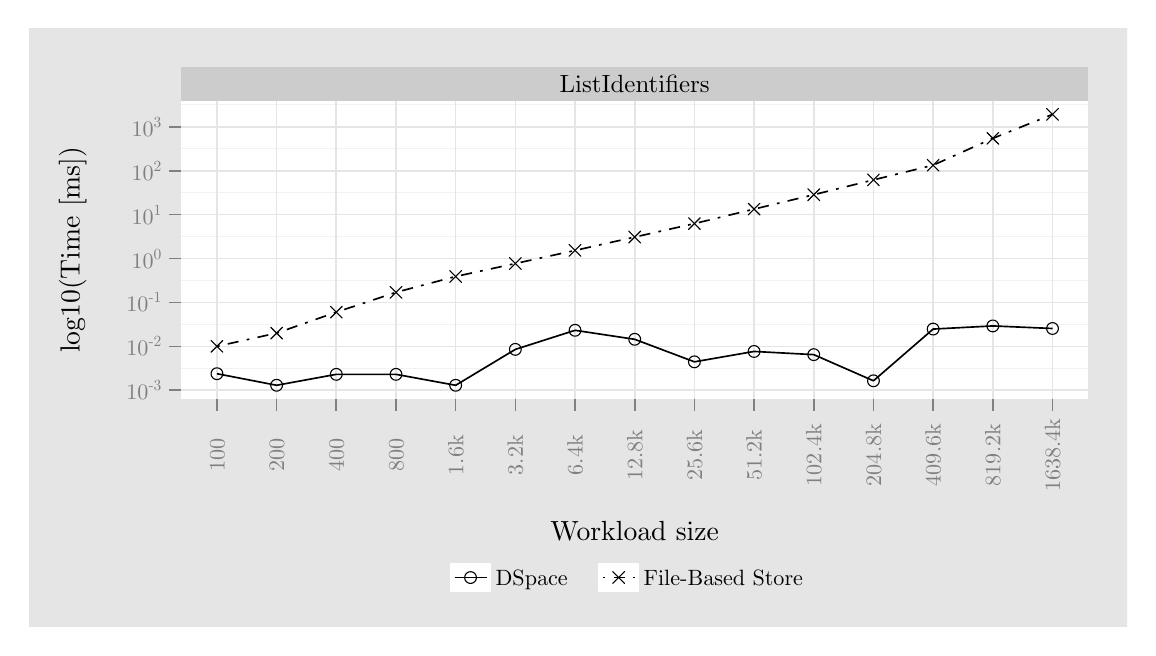
\begin{tikzpicture}[x=1pt,y=1pt]
\definecolor[named]{fillColor}{rgb}{1.00,1.00,1.00}
\path[use as bounding box,fill=fillColor,fill opacity=0.00] (0,0) rectangle (397.48,216.81);
\begin{scope}
\path[clip] (  0.00,  0.00) rectangle (397.48,216.81);
\definecolor[named]{drawColor}{rgb}{1.00,1.00,1.00}
\definecolor[named]{fillColor}{rgb}{0.90,0.90,0.90}

\path[draw=drawColor,line width= 0.6pt,line join=round,line cap=round,fill=fillColor] (  0.00,  0.00) rectangle (397.48,216.81);
\end{scope}
\begin{scope}
\path[clip] ( 55.45, 82.69) rectangle (383.26,190.36);
\definecolor[named]{fillColor}{rgb}{1.00,1.00,1.00}

\path[fill=fillColor] ( 55.45, 82.69) rectangle (383.26,190.36);
\definecolor[named]{drawColor}{rgb}{0.95,0.95,0.95}

\path[draw=drawColor,line width= 0.3pt,line join=round] ( 55.45, 93.73) --
	(383.26, 93.73);

\path[draw=drawColor,line width= 0.3pt,line join=round] ( 55.45,109.59) --
	(383.26,109.59);

\path[draw=drawColor,line width= 0.3pt,line join=round] ( 55.45,125.45) --
	(383.26,125.45);

\path[draw=drawColor,line width= 0.3pt,line join=round] ( 55.45,141.31) --
	(383.26,141.31);

\path[draw=drawColor,line width= 0.3pt,line join=round] ( 55.45,157.17) --
	(383.26,157.17);

\path[draw=drawColor,line width= 0.3pt,line join=round] ( 55.45,173.03) --
	(383.26,173.03);

\path[draw=drawColor,line width= 0.3pt,line join=round] ( 55.45,188.90) --
	(383.26,188.90);
\definecolor[named]{drawColor}{rgb}{0.90,0.90,0.90}

\path[draw=drawColor,line width= 0.6pt,line join=round] ( 55.45, 85.80) --
	(383.26, 85.80);

\path[draw=drawColor,line width= 0.6pt,line join=round] ( 55.45,101.66) --
	(383.26,101.66);

\path[draw=drawColor,line width= 0.6pt,line join=round] ( 55.45,117.52) --
	(383.26,117.52);

\path[draw=drawColor,line width= 0.6pt,line join=round] ( 55.45,133.38) --
	(383.26,133.38);

\path[draw=drawColor,line width= 0.6pt,line join=round] ( 55.45,149.24) --
	(383.26,149.24);

\path[draw=drawColor,line width= 0.6pt,line join=round] ( 55.45,165.10) --
	(383.26,165.10);

\path[draw=drawColor,line width= 0.6pt,line join=round] ( 55.45,180.96) --
	(383.26,180.96);

\path[draw=drawColor,line width= 0.6pt,line join=round] ( 68.39, 82.69) --
	( 68.39,190.36);

\path[draw=drawColor,line width= 0.6pt,line join=round] ( 89.95, 82.69) --
	( 89.95,190.36);

\path[draw=drawColor,line width= 0.6pt,line join=round] (111.52, 82.69) --
	(111.52,190.36);

\path[draw=drawColor,line width= 0.6pt,line join=round] (133.09, 82.69) --
	(133.09,190.36);

\path[draw=drawColor,line width= 0.6pt,line join=round] (154.65, 82.69) --
	(154.65,190.36);

\path[draw=drawColor,line width= 0.6pt,line join=round] (176.22, 82.69) --
	(176.22,190.36);

\path[draw=drawColor,line width= 0.6pt,line join=round] (197.79, 82.69) --
	(197.79,190.36);

\path[draw=drawColor,line width= 0.6pt,line join=round] (219.35, 82.69) --
	(219.35,190.36);

\path[draw=drawColor,line width= 0.6pt,line join=round] (240.92, 82.69) --
	(240.92,190.36);

\path[draw=drawColor,line width= 0.6pt,line join=round] (262.49, 82.69) --
	(262.49,190.36);

\path[draw=drawColor,line width= 0.6pt,line join=round] (284.05, 82.69) --
	(284.05,190.36);

\path[draw=drawColor,line width= 0.6pt,line join=round] (305.62, 82.69) --
	(305.62,190.36);

\path[draw=drawColor,line width= 0.6pt,line join=round] (327.19, 82.69) --
	(327.19,190.36);

\path[draw=drawColor,line width= 0.6pt,line join=round] (348.75, 82.69) --
	(348.75,190.36);

\path[draw=drawColor,line width= 0.6pt,line join=round] (370.32, 82.69) --
	(370.32,190.36);
\definecolor[named]{drawColor}{rgb}{0.00,0.00,0.00}

\path[draw=drawColor,line width= 0.6pt,line join=round] ( 68.39, 91.77) --
	( 89.95, 87.59) --
	(111.52, 91.54) --
	(133.09, 91.54) --
	(154.65, 87.58) --
	(176.22,100.56) --
	(197.79,107.45) --
	(219.35,104.20) --
	(240.92, 96.06) --
	(262.49, 99.81) --
	(284.05, 98.66) --
	(305.62, 89.21) --
	(327.19,107.90) --
	(348.75,109.03) --
	(370.32,108.11);

\path[draw=drawColor,line width= 0.6pt,dash pattern=on 1pt off 3pt on 4pt off 3pt ,line join=round] ( 68.39,101.66) --
	( 89.95,106.43) --
	(111.52,114.00) --
	(133.09,121.18) --
	(154.65,126.90) --
	(176.22,131.58) --
	(197.79,136.31) --
	(219.35,141.15) --
	(240.92,146.01) --
	(262.49,151.25) --
	(284.05,156.45) --
	(305.62,161.80) --
	(327.19,167.12) --
	(348.75,176.82) --
	(370.32,185.47);

\path[draw=drawColor,line width= 0.4pt,line join=round,line cap=round] ( 68.39, 91.77) circle (  2.13);

\path[draw=drawColor,line width= 0.4pt,line join=round,line cap=round] ( 89.95, 87.59) circle (  2.13);

\path[draw=drawColor,line width= 0.4pt,line join=round,line cap=round] (111.52, 91.54) circle (  2.13);

\path[draw=drawColor,line width= 0.4pt,line join=round,line cap=round] (133.09, 91.54) circle (  2.13);

\path[draw=drawColor,line width= 0.4pt,line join=round,line cap=round] (154.65, 87.58) circle (  2.13);

\path[draw=drawColor,line width= 0.4pt,line join=round,line cap=round] (176.22,100.56) circle (  2.13);

\path[draw=drawColor,line width= 0.4pt,line join=round,line cap=round] (197.79,107.45) circle (  2.13);

\path[draw=drawColor,line width= 0.4pt,line join=round,line cap=round] (219.35,104.20) circle (  2.13);

\path[draw=drawColor,line width= 0.4pt,line join=round,line cap=round] (240.92, 96.06) circle (  2.13);

\path[draw=drawColor,line width= 0.4pt,line join=round,line cap=round] (262.49, 99.81) circle (  2.13);

\path[draw=drawColor,line width= 0.4pt,line join=round,line cap=round] (284.05, 98.66) circle (  2.13);

\path[draw=drawColor,line width= 0.4pt,line join=round,line cap=round] (305.62, 89.21) circle (  2.13);

\path[draw=drawColor,line width= 0.4pt,line join=round,line cap=round] (327.19,107.90) circle (  2.13);

\path[draw=drawColor,line width= 0.4pt,line join=round,line cap=round] (348.75,109.03) circle (  2.13);

\path[draw=drawColor,line width= 0.4pt,line join=round,line cap=round] (370.32,108.11) circle (  2.13);

\path[draw=drawColor,line width= 0.4pt,line join=round,line cap=round,fill=fillColor] ( 66.25, 99.53) -- ( 70.52,103.79);

\path[draw=drawColor,line width= 0.4pt,line join=round,line cap=round,fill=fillColor] ( 66.25,103.79) -- ( 70.52, 99.53);

\path[draw=drawColor,line width= 0.4pt,line join=round,line cap=round,fill=fillColor] ( 87.82,104.30) -- ( 92.09,108.57);

\path[draw=drawColor,line width= 0.4pt,line join=round,line cap=round,fill=fillColor] ( 87.82,108.57) -- ( 92.09,104.30);

\path[draw=drawColor,line width= 0.4pt,line join=round,line cap=round,fill=fillColor] (109.39,111.87) -- (113.66,116.14);

\path[draw=drawColor,line width= 0.4pt,line join=round,line cap=round,fill=fillColor] (109.39,116.14) -- (113.66,111.87);

\path[draw=drawColor,line width= 0.4pt,line join=round,line cap=round,fill=fillColor] (130.95,119.04) -- (135.22,123.31);

\path[draw=drawColor,line width= 0.4pt,line join=round,line cap=round,fill=fillColor] (130.95,123.31) -- (135.22,119.04);

\path[draw=drawColor,line width= 0.4pt,line join=round,line cap=round,fill=fillColor] (152.52,124.76) -- (156.79,129.03);

\path[draw=drawColor,line width= 0.4pt,line join=round,line cap=round,fill=fillColor] (152.52,129.03) -- (156.79,124.76);

\path[draw=drawColor,line width= 0.4pt,line join=round,line cap=round,fill=fillColor] (174.09,129.45) -- (178.35,133.72);

\path[draw=drawColor,line width= 0.4pt,line join=round,line cap=round,fill=fillColor] (174.09,133.72) -- (178.35,129.45);

\path[draw=drawColor,line width= 0.4pt,line join=round,line cap=round,fill=fillColor] (195.65,134.18) -- (199.92,138.45);

\path[draw=drawColor,line width= 0.4pt,line join=round,line cap=round,fill=fillColor] (195.65,138.45) -- (199.92,134.18);

\path[draw=drawColor,line width= 0.4pt,line join=round,line cap=round,fill=fillColor] (217.22,139.02) -- (221.49,143.29);

\path[draw=drawColor,line width= 0.4pt,line join=round,line cap=round,fill=fillColor] (217.22,143.29) -- (221.49,139.02);

\path[draw=drawColor,line width= 0.4pt,line join=round,line cap=round,fill=fillColor] (238.79,143.87) -- (243.05,148.14);

\path[draw=drawColor,line width= 0.4pt,line join=round,line cap=round,fill=fillColor] (238.79,148.14) -- (243.05,143.87);

\path[draw=drawColor,line width= 0.4pt,line join=round,line cap=round,fill=fillColor] (260.35,149.11) -- (264.62,153.38);

\path[draw=drawColor,line width= 0.4pt,line join=round,line cap=round,fill=fillColor] (260.35,153.38) -- (264.62,149.11);

\path[draw=drawColor,line width= 0.4pt,line join=round,line cap=round,fill=fillColor] (281.92,154.31) -- (286.19,158.58);

\path[draw=drawColor,line width= 0.4pt,line join=round,line cap=round,fill=fillColor] (281.92,158.58) -- (286.19,154.31);

\path[draw=drawColor,line width= 0.4pt,line join=round,line cap=round,fill=fillColor] (303.49,159.66) -- (307.75,163.93);

\path[draw=drawColor,line width= 0.4pt,line join=round,line cap=round,fill=fillColor] (303.49,163.93) -- (307.75,159.66);

\path[draw=drawColor,line width= 0.4pt,line join=round,line cap=round,fill=fillColor] (325.05,164.98) -- (329.32,169.25);

\path[draw=drawColor,line width= 0.4pt,line join=round,line cap=round,fill=fillColor] (325.05,169.25) -- (329.32,164.98);

\path[draw=drawColor,line width= 0.4pt,line join=round,line cap=round,fill=fillColor] (346.62,174.69) -- (350.89,178.96);

\path[draw=drawColor,line width= 0.4pt,line join=round,line cap=round,fill=fillColor] (346.62,178.96) -- (350.89,174.69);

\path[draw=drawColor,line width= 0.4pt,line join=round,line cap=round,fill=fillColor] (368.18,183.33) -- (372.45,187.60);

\path[draw=drawColor,line width= 0.4pt,line join=round,line cap=round,fill=fillColor] (368.18,187.60) -- (372.45,183.33);
\end{scope}
\begin{scope}
\path[clip] (  0.00,  0.00) rectangle (397.48,216.81);
\definecolor[named]{fillColor}{rgb}{0.80,0.80,0.80}

\path[fill=fillColor] ( 55.45,190.36) rectangle (383.26,202.58);
\definecolor[named]{drawColor}{rgb}{0.00,0.00,0.00}

\node[text=drawColor,anchor=base,inner sep=0pt, outer sep=0pt, scale=  0.90] at (219.35,193.37) {ListIdentifiers};
\end{scope}
\begin{scope}
\path[clip] (  0.00,  0.00) rectangle (397.48,216.81);
\definecolor[named]{drawColor}{rgb}{0.50,0.50,0.50}

\node[text=drawColor,anchor=base west,inner sep=0pt, outer sep=0pt, scale=  0.80] at ( 35.67, 82.37) {10};

\node[text=drawColor,anchor=base west,inner sep=0pt, outer sep=0pt, scale=  0.56] at ( 43.67, 85.64) {-};

\node[text=drawColor,anchor=base west,inner sep=0pt, outer sep=0pt, scale=  0.56] at ( 45.54, 85.64) {3};

\node[text=drawColor,anchor=base west,inner sep=0pt, outer sep=0pt, scale=  0.80] at ( 35.67, 98.23) {10};

\node[text=drawColor,anchor=base west,inner sep=0pt, outer sep=0pt, scale=  0.56] at ( 43.67,101.50) {-};

\node[text=drawColor,anchor=base west,inner sep=0pt, outer sep=0pt, scale=  0.56] at ( 45.54,101.50) {2};

\node[text=drawColor,anchor=base west,inner sep=0pt, outer sep=0pt, scale=  0.80] at ( 35.67,114.09) {10};

\node[text=drawColor,anchor=base west,inner sep=0pt, outer sep=0pt, scale=  0.56] at ( 43.67,117.36) {-};

\node[text=drawColor,anchor=base west,inner sep=0pt, outer sep=0pt, scale=  0.56] at ( 45.54,117.36) {1};

\node[text=drawColor,anchor=base west,inner sep=0pt, outer sep=0pt, scale=  0.80] at ( 37.54,129.95) {10};

\node[text=drawColor,anchor=base west,inner sep=0pt, outer sep=0pt, scale=  0.56] at ( 45.54,133.22) {0};

\node[text=drawColor,anchor=base west,inner sep=0pt, outer sep=0pt, scale=  0.80] at ( 37.54,145.81) {10};

\node[text=drawColor,anchor=base west,inner sep=0pt, outer sep=0pt, scale=  0.56] at ( 45.54,149.08) {1};

\node[text=drawColor,anchor=base west,inner sep=0pt, outer sep=0pt, scale=  0.80] at ( 37.54,161.67) {10};

\node[text=drawColor,anchor=base west,inner sep=0pt, outer sep=0pt, scale=  0.56] at ( 45.54,164.94) {2};

\node[text=drawColor,anchor=base west,inner sep=0pt, outer sep=0pt, scale=  0.80] at ( 37.54,177.53) {10};

\node[text=drawColor,anchor=base west,inner sep=0pt, outer sep=0pt, scale=  0.56] at ( 45.54,180.80) {3};
\end{scope}
\begin{scope}
\path[clip] (  0.00,  0.00) rectangle (397.48,216.81);
\definecolor[named]{drawColor}{rgb}{0.50,0.50,0.50}

\path[draw=drawColor,line width= 0.6pt,line join=round] ( 51.18, 85.80) --
	( 55.45, 85.80);

\path[draw=drawColor,line width= 0.6pt,line join=round] ( 51.18,101.66) --
	( 55.45,101.66);

\path[draw=drawColor,line width= 0.6pt,line join=round] ( 51.18,117.52) --
	( 55.45,117.52);

\path[draw=drawColor,line width= 0.6pt,line join=round] ( 51.18,133.38) --
	( 55.45,133.38);

\path[draw=drawColor,line width= 0.6pt,line join=round] ( 51.18,149.24) --
	( 55.45,149.24);

\path[draw=drawColor,line width= 0.6pt,line join=round] ( 51.18,165.10) --
	( 55.45,165.10);

\path[draw=drawColor,line width= 0.6pt,line join=round] ( 51.18,180.96) --
	( 55.45,180.96);
\end{scope}
\begin{scope}
\path[clip] (  0.00,  0.00) rectangle (397.48,216.81);
\definecolor[named]{drawColor}{rgb}{0.50,0.50,0.50}

\path[draw=drawColor,line width= 0.6pt,line join=round] ( 68.39, 78.42) --
	( 68.39, 82.69);

\path[draw=drawColor,line width= 0.6pt,line join=round] ( 89.95, 78.42) --
	( 89.95, 82.69);

\path[draw=drawColor,line width= 0.6pt,line join=round] (111.52, 78.42) --
	(111.52, 82.69);

\path[draw=drawColor,line width= 0.6pt,line join=round] (133.09, 78.42) --
	(133.09, 82.69);

\path[draw=drawColor,line width= 0.6pt,line join=round] (154.65, 78.42) --
	(154.65, 82.69);

\path[draw=drawColor,line width= 0.6pt,line join=round] (176.22, 78.42) --
	(176.22, 82.69);

\path[draw=drawColor,line width= 0.6pt,line join=round] (197.79, 78.42) --
	(197.79, 82.69);

\path[draw=drawColor,line width= 0.6pt,line join=round] (219.35, 78.42) --
	(219.35, 82.69);

\path[draw=drawColor,line width= 0.6pt,line join=round] (240.92, 78.42) --
	(240.92, 82.69);

\path[draw=drawColor,line width= 0.6pt,line join=round] (262.49, 78.42) --
	(262.49, 82.69);

\path[draw=drawColor,line width= 0.6pt,line join=round] (284.05, 78.42) --
	(284.05, 82.69);

\path[draw=drawColor,line width= 0.6pt,line join=round] (305.62, 78.42) --
	(305.62, 82.69);

\path[draw=drawColor,line width= 0.6pt,line join=round] (327.19, 78.42) --
	(327.19, 82.69);

\path[draw=drawColor,line width= 0.6pt,line join=round] (348.75, 78.42) --
	(348.75, 82.69);

\path[draw=drawColor,line width= 0.6pt,line join=round] (370.32, 78.42) --
	(370.32, 82.69);
\end{scope}
\begin{scope}
\path[clip] (  0.00,  0.00) rectangle (397.48,216.81);
\definecolor[named]{drawColor}{rgb}{0.50,0.50,0.50}

\node[text=drawColor,rotate= 90.00,anchor=base,inner sep=0pt, outer sep=0pt, scale=  0.80] at ( 71.14, 62.36) {100};

\node[text=drawColor,rotate= 90.00,anchor=base,inner sep=0pt, outer sep=0pt, scale=  0.80] at ( 92.71, 62.36) {200};

\node[text=drawColor,rotate= 90.00,anchor=base,inner sep=0pt, outer sep=0pt, scale=  0.80] at (114.28, 62.36) {400};

\node[text=drawColor,rotate= 90.00,anchor=base,inner sep=0pt, outer sep=0pt, scale=  0.80] at (135.84, 62.36) {800};

\node[text=drawColor,rotate= 90.00,anchor=base,inner sep=0pt, outer sep=0pt, scale=  0.80] at (157.41, 62.36) {1.6k};

\node[text=drawColor,rotate= 90.00,anchor=base,inner sep=0pt, outer sep=0pt, scale=  0.80] at (178.98, 62.36) {3.2k};

\node[text=drawColor,rotate= 90.00,anchor=base,inner sep=0pt, outer sep=0pt, scale=  0.80] at (200.54, 62.36) {6.4k};

\node[text=drawColor,rotate= 90.00,anchor=base,inner sep=0pt, outer sep=0pt, scale=  0.80] at (222.11, 62.36) {12.8k};

\node[text=drawColor,rotate= 90.00,anchor=base,inner sep=0pt, outer sep=0pt, scale=  0.80] at (243.67, 62.36) {25.6k};

\node[text=drawColor,rotate= 90.00,anchor=base,inner sep=0pt, outer sep=0pt, scale=  0.80] at (265.24, 62.36) {51.2k};

\node[text=drawColor,rotate= 90.00,anchor=base,inner sep=0pt, outer sep=0pt, scale=  0.80] at (286.81, 62.36) {102.4k};

\node[text=drawColor,rotate= 90.00,anchor=base,inner sep=0pt, outer sep=0pt, scale=  0.80] at (308.37, 62.36) {204.8k};

\node[text=drawColor,rotate= 90.00,anchor=base,inner sep=0pt, outer sep=0pt, scale=  0.80] at (329.94, 62.36) {409.6k};

\node[text=drawColor,rotate= 90.00,anchor=base,inner sep=0pt, outer sep=0pt, scale=  0.80] at (351.51, 62.36) {819.2k};

\node[text=drawColor,rotate= 90.00,anchor=base,inner sep=0pt, outer sep=0pt, scale=  0.80] at (373.07, 62.36) {1638.4k};
\end{scope}
\begin{scope}
\path[clip] (  0.00,  0.00) rectangle (397.48,216.81);
\definecolor[named]{drawColor}{rgb}{0.00,0.00,0.00}

\node[text=drawColor,anchor=base,inner sep=0pt, outer sep=0pt, scale=  1.00] at (219.35, 31.41) {Workload size};
\end{scope}
\begin{scope}
\path[clip] (  0.00,  0.00) rectangle (397.48,216.81);
\definecolor[named]{drawColor}{rgb}{0.00,0.00,0.00}

\node[text=drawColor,rotate= 90.00,anchor=base,inner sep=0pt, outer sep=0pt, scale=  1.00] at ( 18.80,136.53) {log10(Time [ms])};
\end{scope}
\begin{scope}
\path[clip] (  0.00,  0.00) rectangle (397.48,216.81);
\definecolor[named]{fillColor}{rgb}{0.90,0.90,0.90}

\path[fill=fillColor] (144.93,  8.87) rectangle (293.78, 27.36);
\end{scope}
\begin{scope}
\path[clip] (  0.00,  0.00) rectangle (397.48,216.81);
\definecolor[named]{drawColor}{rgb}{1.00,1.00,1.00}
\definecolor[named]{fillColor}{rgb}{1.00,1.00,1.00}

\path[draw=drawColor,line width= 0.6pt,line join=round,line cap=round,fill=fillColor] (152.81, 13.14) rectangle (167.26, 23.09);
\end{scope}
\begin{scope}
\path[clip] (  0.00,  0.00) rectangle (397.48,216.81);
\definecolor[named]{drawColor}{rgb}{0.00,0.00,0.00}

\path[draw=drawColor,line width= 0.6pt,line join=round] (154.25, 18.11) -- (165.82, 18.11);
\end{scope}
\begin{scope}
\path[clip] (  0.00,  0.00) rectangle (397.48,216.81);
\definecolor[named]{drawColor}{rgb}{0.00,0.00,0.00}

\path[draw=drawColor,line width= 0.4pt,line join=round,line cap=round] (160.03, 18.11) circle (  2.13);
\end{scope}
\begin{scope}
\path[clip] (  0.00,  0.00) rectangle (397.48,216.81);
\definecolor[named]{drawColor}{rgb}{1.00,1.00,1.00}
\definecolor[named]{fillColor}{rgb}{1.00,1.00,1.00}

\path[draw=drawColor,line width= 0.6pt,line join=round,line cap=round,fill=fillColor] (206.31, 13.14) rectangle (220.77, 23.09);
\end{scope}
\begin{scope}
\path[clip] (  0.00,  0.00) rectangle (397.48,216.81);
\definecolor[named]{drawColor}{rgb}{0.00,0.00,0.00}

\path[draw=drawColor,line width= 0.6pt,dash pattern=on 1pt off 3pt on 4pt off 3pt ,line join=round] (207.76, 18.11) -- (219.32, 18.11);
\end{scope}
\begin{scope}
\path[clip] (  0.00,  0.00) rectangle (397.48,216.81);
\definecolor[named]{drawColor}{rgb}{0.00,0.00,0.00}
\definecolor[named]{fillColor}{rgb}{1.00,1.00,1.00}

\path[draw=drawColor,line width= 0.4pt,line join=round,line cap=round,fill=fillColor] (211.41, 15.98) -- (215.67, 20.25);

\path[draw=drawColor,line width= 0.4pt,line join=round,line cap=round,fill=fillColor] (211.41, 20.25) -- (215.67, 15.98);
\end{scope}
\begin{scope}
\path[clip] (  0.00,  0.00) rectangle (397.48,216.81);
\definecolor[named]{drawColor}{rgb}{0.00,0.00,0.00}

\node[text=drawColor,anchor=base west,inner sep=0pt, outer sep=0pt, scale=  0.80] at (169.07, 15.36) {DSpace $\;\;\;$};
\end{scope}
\begin{scope}
\path[clip] (  0.00,  0.00) rectangle (397.48,216.81);
\definecolor[named]{drawColor}{rgb}{0.00,0.00,0.00}

\node[text=drawColor,anchor=base west,inner sep=0pt, outer sep=0pt, scale=  0.80] at (222.57, 15.36) {File-Based Store $\;\;\;$};
\end{scope}
\end{tikzpicture}

 }
\caption[OAI-PMH ListIdentifiers\index{OAI-PMH!Verbs!ListIdentifiers} performance comparison]{OAI-PMH ListIdentifiers\index{OAI-PMH!Verbs!ListIdentifiers} performance comparison.}
 \label{fig:experimentation:performance:comparision:oaipmh-listidentifiers}
\end{figure}

\begin{figure}
 \centering
 \framebox[\textwidth]{%
% Created by tikzDevice version 0.6.2-92-0ad2792 on 2013-03-23 23:12:12
% !TEX encoding = UTF-8 Unicode
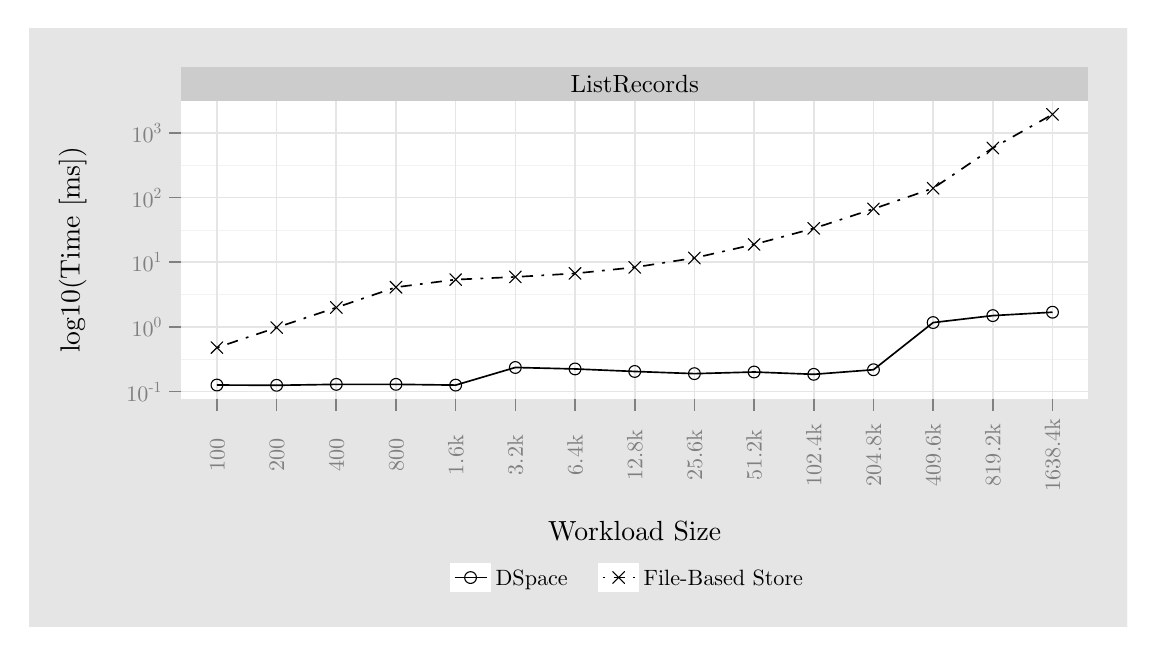
\begin{tikzpicture}[x=1pt,y=1pt]
\definecolor[named]{fillColor}{rgb}{1.00,1.00,1.00}
\path[use as bounding box,fill=fillColor,fill opacity=0.00] (0,0) rectangle (397.48,216.81);
\begin{scope}
\path[clip] (  0.00,  0.00) rectangle (397.48,216.81);
\definecolor[named]{drawColor}{rgb}{1.00,1.00,1.00}
\definecolor[named]{fillColor}{rgb}{0.90,0.90,0.90}

\path[draw=drawColor,line width= 0.6pt,line join=round,line cap=round,fill=fillColor] (  0.00,  0.00) rectangle (397.48,216.81);
\end{scope}
\begin{scope}
\path[clip] ( 55.45, 82.69) rectangle (383.26,190.36);
\definecolor[named]{fillColor}{rgb}{1.00,1.00,1.00}

\path[fill=fillColor] ( 55.45, 82.69) rectangle (383.26,190.36);
\definecolor[named]{drawColor}{rgb}{0.95,0.95,0.95}

\path[draw=drawColor,line width= 0.3pt,line join=round] ( 55.45, 96.96) --
	(383.26, 96.96);

\path[draw=drawColor,line width= 0.3pt,line join=round] ( 55.45,120.33) --
	(383.26,120.33);

\path[draw=drawColor,line width= 0.3pt,line join=round] ( 55.45,143.70) --
	(383.26,143.70);

\path[draw=drawColor,line width= 0.3pt,line join=round] ( 55.45,167.07) --
	(383.26,167.07);
\definecolor[named]{drawColor}{rgb}{0.90,0.90,0.90}

\path[draw=drawColor,line width= 0.6pt,line join=round] ( 55.45, 85.28) --
	(383.26, 85.28);

\path[draw=drawColor,line width= 0.6pt,line join=round] ( 55.45,108.65) --
	(383.26,108.65);

\path[draw=drawColor,line width= 0.6pt,line join=round] ( 55.45,132.02) --
	(383.26,132.02);

\path[draw=drawColor,line width= 0.6pt,line join=round] ( 55.45,155.39) --
	(383.26,155.39);

\path[draw=drawColor,line width= 0.6pt,line join=round] ( 55.45,178.76) --
	(383.26,178.76);

\path[draw=drawColor,line width= 0.6pt,line join=round] ( 68.39, 82.69) --
	( 68.39,190.36);

\path[draw=drawColor,line width= 0.6pt,line join=round] ( 89.95, 82.69) --
	( 89.95,190.36);

\path[draw=drawColor,line width= 0.6pt,line join=round] (111.52, 82.69) --
	(111.52,190.36);

\path[draw=drawColor,line width= 0.6pt,line join=round] (133.09, 82.69) --
	(133.09,190.36);

\path[draw=drawColor,line width= 0.6pt,line join=round] (154.65, 82.69) --
	(154.65,190.36);

\path[draw=drawColor,line width= 0.6pt,line join=round] (176.22, 82.69) --
	(176.22,190.36);

\path[draw=drawColor,line width= 0.6pt,line join=round] (197.79, 82.69) --
	(197.79,190.36);

\path[draw=drawColor,line width= 0.6pt,line join=round] (219.35, 82.69) --
	(219.35,190.36);

\path[draw=drawColor,line width= 0.6pt,line join=round] (240.92, 82.69) --
	(240.92,190.36);

\path[draw=drawColor,line width= 0.6pt,line join=round] (262.49, 82.69) --
	(262.49,190.36);

\path[draw=drawColor,line width= 0.6pt,line join=round] (284.05, 82.69) --
	(284.05,190.36);

\path[draw=drawColor,line width= 0.6pt,line join=round] (305.62, 82.69) --
	(305.62,190.36);

\path[draw=drawColor,line width= 0.6pt,line join=round] (327.19, 82.69) --
	(327.19,190.36);

\path[draw=drawColor,line width= 0.6pt,line join=round] (348.75, 82.69) --
	(348.75,190.36);

\path[draw=drawColor,line width= 0.6pt,line join=round] (370.32, 82.69) --
	(370.32,190.36);
\definecolor[named]{drawColor}{rgb}{0.00,0.00,0.00}

\path[draw=drawColor,line width= 0.6pt,line join=round] ( 68.39, 87.68) --
	( 89.95, 87.58) --
	(111.52, 87.92) --
	(133.09, 87.93) --
	(154.65, 87.65) --
	(176.22, 94.02) --
	(197.79, 93.49) --
	(219.35, 92.58) --
	(240.92, 91.79) --
	(262.49, 92.38) --
	(284.05, 91.55) --
	(305.62, 93.20) --
	(327.19,110.25) --
	(348.75,112.76) --
	(370.32,113.99);

\path[draw=drawColor,line width= 0.6pt,dash pattern=on 1pt off 3pt on 4pt off 3pt ,line join=round] ( 68.39,101.20) --
	( 89.95,108.44) --
	(111.52,115.68) --
	(133.09,123.02) --
	(154.65,125.78) --
	(176.22,126.73) --
	(197.79,128.00) --
	(219.35,130.21) --
	(240.92,133.59) --
	(262.49,138.48) --
	(284.05,144.28) --
	(305.62,151.32) --
	(327.19,158.78) --
	(348.75,173.34) --
	(370.32,185.47);

\path[draw=drawColor,line width= 0.4pt,line join=round,line cap=round] ( 68.39, 87.68) circle (  2.13);

\path[draw=drawColor,line width= 0.4pt,line join=round,line cap=round] ( 89.95, 87.58) circle (  2.13);

\path[draw=drawColor,line width= 0.4pt,line join=round,line cap=round] (111.52, 87.92) circle (  2.13);

\path[draw=drawColor,line width= 0.4pt,line join=round,line cap=round] (133.09, 87.93) circle (  2.13);

\path[draw=drawColor,line width= 0.4pt,line join=round,line cap=round] (154.65, 87.65) circle (  2.13);

\path[draw=drawColor,line width= 0.4pt,line join=round,line cap=round] (176.22, 94.02) circle (  2.13);

\path[draw=drawColor,line width= 0.4pt,line join=round,line cap=round] (197.79, 93.49) circle (  2.13);

\path[draw=drawColor,line width= 0.4pt,line join=round,line cap=round] (219.35, 92.58) circle (  2.13);

\path[draw=drawColor,line width= 0.4pt,line join=round,line cap=round] (240.92, 91.79) circle (  2.13);

\path[draw=drawColor,line width= 0.4pt,line join=round,line cap=round] (262.49, 92.38) circle (  2.13);

\path[draw=drawColor,line width= 0.4pt,line join=round,line cap=round] (284.05, 91.55) circle (  2.13);

\path[draw=drawColor,line width= 0.4pt,line join=round,line cap=round] (305.62, 93.20) circle (  2.13);

\path[draw=drawColor,line width= 0.4pt,line join=round,line cap=round] (327.19,110.25) circle (  2.13);

\path[draw=drawColor,line width= 0.4pt,line join=round,line cap=round] (348.75,112.76) circle (  2.13);

\path[draw=drawColor,line width= 0.4pt,line join=round,line cap=round] (370.32,113.99) circle (  2.13);

\path[draw=drawColor,line width= 0.4pt,line join=round,line cap=round,fill=fillColor] ( 66.25, 99.07) -- ( 70.52,103.33);

\path[draw=drawColor,line width= 0.4pt,line join=round,line cap=round,fill=fillColor] ( 66.25,103.33) -- ( 70.52, 99.07);

\path[draw=drawColor,line width= 0.4pt,line join=round,line cap=round,fill=fillColor] ( 87.82,106.31) -- ( 92.09,110.58);

\path[draw=drawColor,line width= 0.4pt,line join=round,line cap=round,fill=fillColor] ( 87.82,110.58) -- ( 92.09,106.31);

\path[draw=drawColor,line width= 0.4pt,line join=round,line cap=round,fill=fillColor] (109.39,113.55) -- (113.66,117.82);

\path[draw=drawColor,line width= 0.4pt,line join=round,line cap=round,fill=fillColor] (109.39,117.82) -- (113.66,113.55);

\path[draw=drawColor,line width= 0.4pt,line join=round,line cap=round,fill=fillColor] (130.95,120.89) -- (135.22,125.15);

\path[draw=drawColor,line width= 0.4pt,line join=round,line cap=round,fill=fillColor] (130.95,125.15) -- (135.22,120.89);

\path[draw=drawColor,line width= 0.4pt,line join=round,line cap=round,fill=fillColor] (152.52,123.65) -- (156.79,127.92);

\path[draw=drawColor,line width= 0.4pt,line join=round,line cap=round,fill=fillColor] (152.52,127.92) -- (156.79,123.65);

\path[draw=drawColor,line width= 0.4pt,line join=round,line cap=round,fill=fillColor] (174.09,124.60) -- (178.35,128.87);

\path[draw=drawColor,line width= 0.4pt,line join=round,line cap=round,fill=fillColor] (174.09,128.87) -- (178.35,124.60);

\path[draw=drawColor,line width= 0.4pt,line join=round,line cap=round,fill=fillColor] (195.65,125.87) -- (199.92,130.13);

\path[draw=drawColor,line width= 0.4pt,line join=round,line cap=round,fill=fillColor] (195.65,130.13) -- (199.92,125.87);

\path[draw=drawColor,line width= 0.4pt,line join=round,line cap=round,fill=fillColor] (217.22,128.08) -- (221.49,132.35);

\path[draw=drawColor,line width= 0.4pt,line join=round,line cap=round,fill=fillColor] (217.22,132.35) -- (221.49,128.08);

\path[draw=drawColor,line width= 0.4pt,line join=round,line cap=round,fill=fillColor] (238.79,131.46) -- (243.05,135.73);

\path[draw=drawColor,line width= 0.4pt,line join=round,line cap=round,fill=fillColor] (238.79,135.73) -- (243.05,131.46);

\path[draw=drawColor,line width= 0.4pt,line join=round,line cap=round,fill=fillColor] (260.35,136.35) -- (264.62,140.61);

\path[draw=drawColor,line width= 0.4pt,line join=round,line cap=round,fill=fillColor] (260.35,140.61) -- (264.62,136.35);

\path[draw=drawColor,line width= 0.4pt,line join=round,line cap=round,fill=fillColor] (281.92,142.14) -- (286.19,146.41);

\path[draw=drawColor,line width= 0.4pt,line join=round,line cap=round,fill=fillColor] (281.92,146.41) -- (286.19,142.14);

\path[draw=drawColor,line width= 0.4pt,line join=round,line cap=round,fill=fillColor] (303.49,149.18) -- (307.75,153.45);

\path[draw=drawColor,line width= 0.4pt,line join=round,line cap=round,fill=fillColor] (303.49,153.45) -- (307.75,149.18);

\path[draw=drawColor,line width= 0.4pt,line join=round,line cap=round,fill=fillColor] (325.05,156.65) -- (329.32,160.92);

\path[draw=drawColor,line width= 0.4pt,line join=round,line cap=round,fill=fillColor] (325.05,160.92) -- (329.32,156.65);

\path[draw=drawColor,line width= 0.4pt,line join=round,line cap=round,fill=fillColor] (346.62,171.21) -- (350.89,175.48);

\path[draw=drawColor,line width= 0.4pt,line join=round,line cap=round,fill=fillColor] (346.62,175.48) -- (350.89,171.21);

\path[draw=drawColor,line width= 0.4pt,line join=round,line cap=round,fill=fillColor] (368.18,183.33) -- (372.45,187.60);

\path[draw=drawColor,line width= 0.4pt,line join=round,line cap=round,fill=fillColor] (368.18,187.60) -- (372.45,183.33);
\end{scope}
\begin{scope}
\path[clip] (  0.00,  0.00) rectangle (397.48,216.81);
\definecolor[named]{fillColor}{rgb}{0.80,0.80,0.80}

\path[fill=fillColor] ( 55.45,190.36) rectangle (383.26,202.58);
\definecolor[named]{drawColor}{rgb}{0.00,0.00,0.00}

\node[text=drawColor,anchor=base,inner sep=0pt, outer sep=0pt, scale=  0.90] at (219.35,193.37) {ListRecords};
\end{scope}
\begin{scope}
\path[clip] (  0.00,  0.00) rectangle (397.48,216.81);
\definecolor[named]{drawColor}{rgb}{0.50,0.50,0.50}

\node[text=drawColor,anchor=base west,inner sep=0pt, outer sep=0pt, scale=  0.80] at ( 35.67, 81.85) {10};

\node[text=drawColor,anchor=base west,inner sep=0pt, outer sep=0pt, scale=  0.56] at ( 43.67, 85.12) {-};

\node[text=drawColor,anchor=base west,inner sep=0pt, outer sep=0pt, scale=  0.56] at ( 45.54, 85.12) {1};

\node[text=drawColor,anchor=base west,inner sep=0pt, outer sep=0pt, scale=  0.80] at ( 37.54,105.22) {10};

\node[text=drawColor,anchor=base west,inner sep=0pt, outer sep=0pt, scale=  0.56] at ( 45.54,108.49) {0};

\node[text=drawColor,anchor=base west,inner sep=0pt, outer sep=0pt, scale=  0.80] at ( 37.54,128.59) {10};

\node[text=drawColor,anchor=base west,inner sep=0pt, outer sep=0pt, scale=  0.56] at ( 45.54,131.86) {1};

\node[text=drawColor,anchor=base west,inner sep=0pt, outer sep=0pt, scale=  0.80] at ( 37.54,151.96) {10};

\node[text=drawColor,anchor=base west,inner sep=0pt, outer sep=0pt, scale=  0.56] at ( 45.54,155.23) {2};

\node[text=drawColor,anchor=base west,inner sep=0pt, outer sep=0pt, scale=  0.80] at ( 37.54,175.33) {10};

\node[text=drawColor,anchor=base west,inner sep=0pt, outer sep=0pt, scale=  0.56] at ( 45.54,178.60) {3};
\end{scope}
\begin{scope}
\path[clip] (  0.00,  0.00) rectangle (397.48,216.81);
\definecolor[named]{drawColor}{rgb}{0.50,0.50,0.50}

\path[draw=drawColor,line width= 0.6pt,line join=round] ( 51.18, 85.28) --
	( 55.45, 85.28);

\path[draw=drawColor,line width= 0.6pt,line join=round] ( 51.18,108.65) --
	( 55.45,108.65);

\path[draw=drawColor,line width= 0.6pt,line join=round] ( 51.18,132.02) --
	( 55.45,132.02);

\path[draw=drawColor,line width= 0.6pt,line join=round] ( 51.18,155.39) --
	( 55.45,155.39);

\path[draw=drawColor,line width= 0.6pt,line join=round] ( 51.18,178.76) --
	( 55.45,178.76);
\end{scope}
\begin{scope}
\path[clip] (  0.00,  0.00) rectangle (397.48,216.81);
\definecolor[named]{drawColor}{rgb}{0.50,0.50,0.50}

\path[draw=drawColor,line width= 0.6pt,line join=round] ( 68.39, 78.42) --
	( 68.39, 82.69);

\path[draw=drawColor,line width= 0.6pt,line join=round] ( 89.95, 78.42) --
	( 89.95, 82.69);

\path[draw=drawColor,line width= 0.6pt,line join=round] (111.52, 78.42) --
	(111.52, 82.69);

\path[draw=drawColor,line width= 0.6pt,line join=round] (133.09, 78.42) --
	(133.09, 82.69);

\path[draw=drawColor,line width= 0.6pt,line join=round] (154.65, 78.42) --
	(154.65, 82.69);

\path[draw=drawColor,line width= 0.6pt,line join=round] (176.22, 78.42) --
	(176.22, 82.69);

\path[draw=drawColor,line width= 0.6pt,line join=round] (197.79, 78.42) --
	(197.79, 82.69);

\path[draw=drawColor,line width= 0.6pt,line join=round] (219.35, 78.42) --
	(219.35, 82.69);

\path[draw=drawColor,line width= 0.6pt,line join=round] (240.92, 78.42) --
	(240.92, 82.69);

\path[draw=drawColor,line width= 0.6pt,line join=round] (262.49, 78.42) --
	(262.49, 82.69);

\path[draw=drawColor,line width= 0.6pt,line join=round] (284.05, 78.42) --
	(284.05, 82.69);

\path[draw=drawColor,line width= 0.6pt,line join=round] (305.62, 78.42) --
	(305.62, 82.69);

\path[draw=drawColor,line width= 0.6pt,line join=round] (327.19, 78.42) --
	(327.19, 82.69);

\path[draw=drawColor,line width= 0.6pt,line join=round] (348.75, 78.42) --
	(348.75, 82.69);

\path[draw=drawColor,line width= 0.6pt,line join=round] (370.32, 78.42) --
	(370.32, 82.69);
\end{scope}
\begin{scope}
\path[clip] (  0.00,  0.00) rectangle (397.48,216.81);
\definecolor[named]{drawColor}{rgb}{0.50,0.50,0.50}

\node[text=drawColor,rotate= 90.00,anchor=base,inner sep=0pt, outer sep=0pt, scale=  0.80] at ( 71.14, 62.36) {100};

\node[text=drawColor,rotate= 90.00,anchor=base,inner sep=0pt, outer sep=0pt, scale=  0.80] at ( 92.71, 62.36) {200};

\node[text=drawColor,rotate= 90.00,anchor=base,inner sep=0pt, outer sep=0pt, scale=  0.80] at (114.28, 62.36) {400};

\node[text=drawColor,rotate= 90.00,anchor=base,inner sep=0pt, outer sep=0pt, scale=  0.80] at (135.84, 62.36) {800};

\node[text=drawColor,rotate= 90.00,anchor=base,inner sep=0pt, outer sep=0pt, scale=  0.80] at (157.41, 62.36) {1.6k};

\node[text=drawColor,rotate= 90.00,anchor=base,inner sep=0pt, outer sep=0pt, scale=  0.80] at (178.98, 62.36) {3.2k};

\node[text=drawColor,rotate= 90.00,anchor=base,inner sep=0pt, outer sep=0pt, scale=  0.80] at (200.54, 62.36) {6.4k};

\node[text=drawColor,rotate= 90.00,anchor=base,inner sep=0pt, outer sep=0pt, scale=  0.80] at (222.11, 62.36) {12.8k};

\node[text=drawColor,rotate= 90.00,anchor=base,inner sep=0pt, outer sep=0pt, scale=  0.80] at (243.67, 62.36) {25.6k};

\node[text=drawColor,rotate= 90.00,anchor=base,inner sep=0pt, outer sep=0pt, scale=  0.80] at (265.24, 62.36) {51.2k};

\node[text=drawColor,rotate= 90.00,anchor=base,inner sep=0pt, outer sep=0pt, scale=  0.80] at (286.81, 62.36) {102.4k};

\node[text=drawColor,rotate= 90.00,anchor=base,inner sep=0pt, outer sep=0pt, scale=  0.80] at (308.37, 62.36) {204.8k};

\node[text=drawColor,rotate= 90.00,anchor=base,inner sep=0pt, outer sep=0pt, scale=  0.80] at (329.94, 62.36) {409.6k};

\node[text=drawColor,rotate= 90.00,anchor=base,inner sep=0pt, outer sep=0pt, scale=  0.80] at (351.51, 62.36) {819.2k};

\node[text=drawColor,rotate= 90.00,anchor=base,inner sep=0pt, outer sep=0pt, scale=  0.80] at (373.07, 62.36) {1638.4k};
\end{scope}
\begin{scope}
\path[clip] (  0.00,  0.00) rectangle (397.48,216.81);
\definecolor[named]{drawColor}{rgb}{0.00,0.00,0.00}

\node[text=drawColor,anchor=base,inner sep=0pt, outer sep=0pt, scale=  1.00] at (219.35, 31.41) {Workload Size};
\end{scope}
\begin{scope}
\path[clip] (  0.00,  0.00) rectangle (397.48,216.81);
\definecolor[named]{drawColor}{rgb}{0.00,0.00,0.00}

\node[text=drawColor,rotate= 90.00,anchor=base,inner sep=0pt, outer sep=0pt, scale=  1.00] at ( 18.80,136.53) {log10(Time [ms])};
\end{scope}
\begin{scope}
\path[clip] (  0.00,  0.00) rectangle (397.48,216.81);
\definecolor[named]{fillColor}{rgb}{0.90,0.90,0.90}

\path[fill=fillColor] (144.93,  8.87) rectangle (293.78, 27.36);
\end{scope}
\begin{scope}
\path[clip] (  0.00,  0.00) rectangle (397.48,216.81);
\definecolor[named]{drawColor}{rgb}{1.00,1.00,1.00}
\definecolor[named]{fillColor}{rgb}{1.00,1.00,1.00}

\path[draw=drawColor,line width= 0.6pt,line join=round,line cap=round,fill=fillColor] (152.81, 13.14) rectangle (167.26, 23.09);
\end{scope}
\begin{scope}
\path[clip] (  0.00,  0.00) rectangle (397.48,216.81);
\definecolor[named]{drawColor}{rgb}{0.00,0.00,0.00}

\path[draw=drawColor,line width= 0.6pt,line join=round] (154.25, 18.11) -- (165.82, 18.11);
\end{scope}
\begin{scope}
\path[clip] (  0.00,  0.00) rectangle (397.48,216.81);
\definecolor[named]{drawColor}{rgb}{0.00,0.00,0.00}

\path[draw=drawColor,line width= 0.4pt,line join=round,line cap=round] (160.03, 18.11) circle (  2.13);
\end{scope}
\begin{scope}
\path[clip] (  0.00,  0.00) rectangle (397.48,216.81);
\definecolor[named]{drawColor}{rgb}{1.00,1.00,1.00}
\definecolor[named]{fillColor}{rgb}{1.00,1.00,1.00}

\path[draw=drawColor,line width= 0.6pt,line join=round,line cap=round,fill=fillColor] (206.31, 13.14) rectangle (220.77, 23.09);
\end{scope}
\begin{scope}
\path[clip] (  0.00,  0.00) rectangle (397.48,216.81);
\definecolor[named]{drawColor}{rgb}{0.00,0.00,0.00}

\path[draw=drawColor,line width= 0.6pt,dash pattern=on 1pt off 3pt on 4pt off 3pt ,line join=round] (207.76, 18.11) -- (219.32, 18.11);
\end{scope}
\begin{scope}
\path[clip] (  0.00,  0.00) rectangle (397.48,216.81);
\definecolor[named]{drawColor}{rgb}{0.00,0.00,0.00}
\definecolor[named]{fillColor}{rgb}{1.00,1.00,1.00}

\path[draw=drawColor,line width= 0.4pt,line join=round,line cap=round,fill=fillColor] (211.41, 15.98) -- (215.67, 20.25);

\path[draw=drawColor,line width= 0.4pt,line join=round,line cap=round,fill=fillColor] (211.41, 20.25) -- (215.67, 15.98);
\end{scope}
\begin{scope}
\path[clip] (  0.00,  0.00) rectangle (397.48,216.81);
\definecolor[named]{drawColor}{rgb}{0.00,0.00,0.00}

\node[text=drawColor,anchor=base west,inner sep=0pt, outer sep=0pt, scale=  0.80] at (169.07, 15.36) {DSpace $\;\;\;$};
\end{scope}
\begin{scope}
\path[clip] (  0.00,  0.00) rectangle (397.48,216.81);
\definecolor[named]{drawColor}{rgb}{0.00,0.00,0.00}

\node[text=drawColor,anchor=base west,inner sep=0pt, outer sep=0pt, scale=  0.80] at (222.57, 15.36) {File-Based Store $\;\;\;$};
\end{scope}
\end{tikzpicture}

 }
\caption[OAI-PMH ListRecords\index{OAI-PMH!Verbs!ListRecords} performance comparison]{OAI-PMH ListRecords\index{OAI-PMH!Verbs!ListRecords} performance comparison.}
 \label{fig:experimentation:performance:comparision:oaipmh-listrecords}
\end{figure}

\begin{figure}
 \centering
 \framebox[\textwidth]{%
% Created by tikzDevice version 0.6.2-92-0ad2792 on 2013-03-23 23:12:59
% !TEX encoding = UTF-8 Unicode
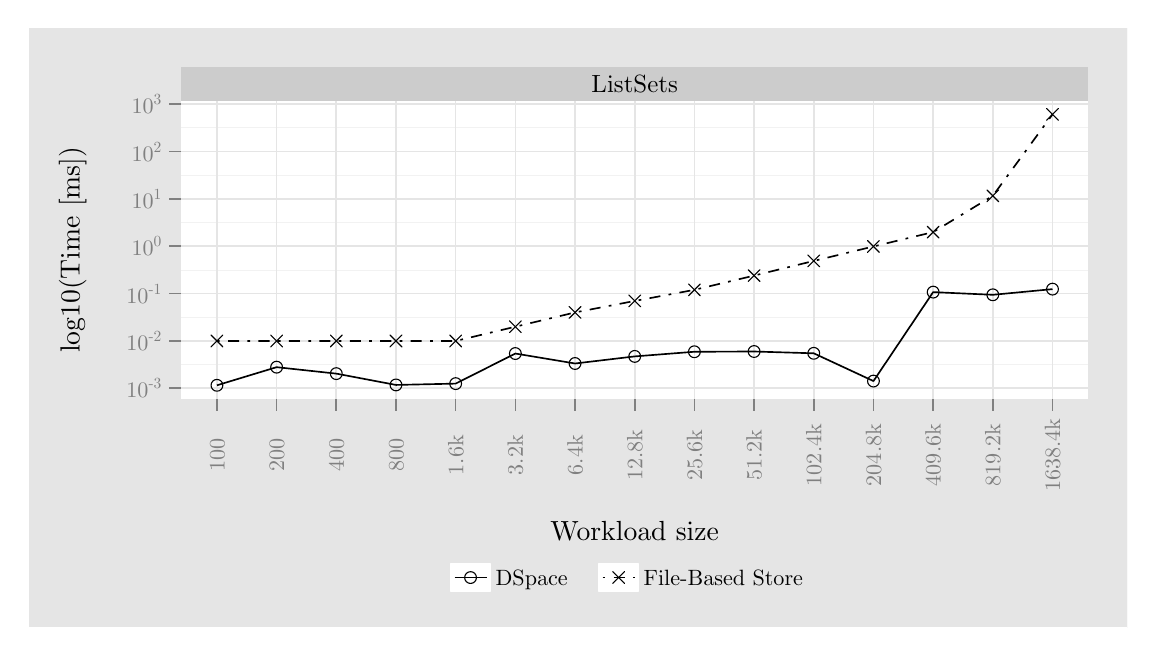
\begin{tikzpicture}[x=1pt,y=1pt]
\definecolor[named]{fillColor}{rgb}{1.00,1.00,1.00}
\path[use as bounding box,fill=fillColor,fill opacity=0.00] (0,0) rectangle (397.48,216.81);
\begin{scope}
\path[clip] (  0.00,  0.00) rectangle (397.48,216.81);
\definecolor[named]{drawColor}{rgb}{1.00,1.00,1.00}
\definecolor[named]{fillColor}{rgb}{0.90,0.90,0.90}

\path[draw=drawColor,line width= 0.6pt,line join=round,line cap=round,fill=fillColor] (  0.00,  0.00) rectangle (397.48,216.81);
\end{scope}
\begin{scope}
\path[clip] ( 55.45, 82.69) rectangle (383.26,190.36);
\definecolor[named]{fillColor}{rgb}{1.00,1.00,1.00}

\path[fill=fillColor] ( 55.45, 82.69) rectangle (383.26,190.36);
\definecolor[named]{drawColor}{rgb}{0.95,0.95,0.95}

\path[draw=drawColor,line width= 0.3pt,line join=round] ( 55.45, 95.05) --
	(383.26, 95.05);

\path[draw=drawColor,line width= 0.3pt,line join=round] ( 55.45,112.16) --
	(383.26,112.16);

\path[draw=drawColor,line width= 0.3pt,line join=round] ( 55.45,129.27) --
	(383.26,129.27);

\path[draw=drawColor,line width= 0.3pt,line join=round] ( 55.45,146.38) --
	(383.26,146.38);

\path[draw=drawColor,line width= 0.3pt,line join=round] ( 55.45,163.49) --
	(383.26,163.49);

\path[draw=drawColor,line width= 0.3pt,line join=round] ( 55.45,180.60) --
	(383.26,180.60);
\definecolor[named]{drawColor}{rgb}{0.90,0.90,0.90}

\path[draw=drawColor,line width= 0.6pt,line join=round] ( 55.45, 86.49) --
	(383.26, 86.49);

\path[draw=drawColor,line width= 0.6pt,line join=round] ( 55.45,103.60) --
	(383.26,103.60);

\path[draw=drawColor,line width= 0.6pt,line join=round] ( 55.45,120.71) --
	(383.26,120.71);

\path[draw=drawColor,line width= 0.6pt,line join=round] ( 55.45,137.82) --
	(383.26,137.82);

\path[draw=drawColor,line width= 0.6pt,line join=round] ( 55.45,154.93) --
	(383.26,154.93);

\path[draw=drawColor,line width= 0.6pt,line join=round] ( 55.45,172.04) --
	(383.26,172.04);

\path[draw=drawColor,line width= 0.6pt,line join=round] ( 55.45,189.15) --
	(383.26,189.15);

\path[draw=drawColor,line width= 0.6pt,line join=round] ( 68.39, 82.69) --
	( 68.39,190.36);

\path[draw=drawColor,line width= 0.6pt,line join=round] ( 89.95, 82.69) --
	( 89.95,190.36);

\path[draw=drawColor,line width= 0.6pt,line join=round] (111.52, 82.69) --
	(111.52,190.36);

\path[draw=drawColor,line width= 0.6pt,line join=round] (133.09, 82.69) --
	(133.09,190.36);

\path[draw=drawColor,line width= 0.6pt,line join=round] (154.65, 82.69) --
	(154.65,190.36);

\path[draw=drawColor,line width= 0.6pt,line join=round] (176.22, 82.69) --
	(176.22,190.36);

\path[draw=drawColor,line width= 0.6pt,line join=round] (197.79, 82.69) --
	(197.79,190.36);

\path[draw=drawColor,line width= 0.6pt,line join=round] (219.35, 82.69) --
	(219.35,190.36);

\path[draw=drawColor,line width= 0.6pt,line join=round] (240.92, 82.69) --
	(240.92,190.36);

\path[draw=drawColor,line width= 0.6pt,line join=round] (262.49, 82.69) --
	(262.49,190.36);

\path[draw=drawColor,line width= 0.6pt,line join=round] (284.05, 82.69) --
	(284.05,190.36);

\path[draw=drawColor,line width= 0.6pt,line join=round] (305.62, 82.69) --
	(305.62,190.36);

\path[draw=drawColor,line width= 0.6pt,line join=round] (327.19, 82.69) --
	(327.19,190.36);

\path[draw=drawColor,line width= 0.6pt,line join=round] (348.75, 82.69) --
	(348.75,190.36);

\path[draw=drawColor,line width= 0.6pt,line join=round] (370.32, 82.69) --
	(370.32,190.36);
\definecolor[named]{drawColor}{rgb}{0.00,0.00,0.00}

\path[draw=drawColor,line width= 0.6pt,line join=round] ( 68.39, 87.58) --
	( 89.95, 94.13) --
	(111.52, 91.80) --
	(133.09, 87.71) --
	(154.65, 88.19) --
	(176.22, 99.06) --
	(197.79, 95.46) --
	(219.35, 98.02) --
	(240.92, 99.70) --
	(262.49, 99.79) --
	(284.05, 99.14) --
	(305.62, 89.11) --
	(327.19,121.25) --
	(348.75,120.28) --
	(370.32,122.33);

\path[draw=drawColor,line width= 0.6pt,dash pattern=on 1pt off 3pt on 4pt off 3pt ,line join=round] ( 68.39,103.60) --
	( 89.95,103.60) --
	(111.52,103.60) --
	(133.09,103.60) --
	(154.65,103.60) --
	(176.22,108.75) --
	(197.79,113.91) --
	(219.35,118.06) --
	(240.92,122.07) --
	(262.49,127.22) --
	(284.05,132.52) --
	(305.62,137.75) --
	(327.19,142.94) --
	(348.75,156.04) --
	(370.32,185.47);

\path[draw=drawColor,line width= 0.4pt,line join=round,line cap=round] ( 68.39, 87.58) circle (  2.13);

\path[draw=drawColor,line width= 0.4pt,line join=round,line cap=round] ( 89.95, 94.13) circle (  2.13);

\path[draw=drawColor,line width= 0.4pt,line join=round,line cap=round] (111.52, 91.80) circle (  2.13);

\path[draw=drawColor,line width= 0.4pt,line join=round,line cap=round] (133.09, 87.71) circle (  2.13);

\path[draw=drawColor,line width= 0.4pt,line join=round,line cap=round] (154.65, 88.19) circle (  2.13);

\path[draw=drawColor,line width= 0.4pt,line join=round,line cap=round] (176.22, 99.06) circle (  2.13);

\path[draw=drawColor,line width= 0.4pt,line join=round,line cap=round] (197.79, 95.46) circle (  2.13);

\path[draw=drawColor,line width= 0.4pt,line join=round,line cap=round] (219.35, 98.02) circle (  2.13);

\path[draw=drawColor,line width= 0.4pt,line join=round,line cap=round] (240.92, 99.70) circle (  2.13);

\path[draw=drawColor,line width= 0.4pt,line join=round,line cap=round] (262.49, 99.79) circle (  2.13);

\path[draw=drawColor,line width= 0.4pt,line join=round,line cap=round] (284.05, 99.14) circle (  2.13);

\path[draw=drawColor,line width= 0.4pt,line join=round,line cap=round] (305.62, 89.11) circle (  2.13);

\path[draw=drawColor,line width= 0.4pt,line join=round,line cap=round] (327.19,121.25) circle (  2.13);

\path[draw=drawColor,line width= 0.4pt,line join=round,line cap=round] (348.75,120.28) circle (  2.13);

\path[draw=drawColor,line width= 0.4pt,line join=round,line cap=round] (370.32,122.33) circle (  2.13);

\path[draw=drawColor,line width= 0.4pt,line join=round,line cap=round,fill=fillColor] ( 66.25,101.47) -- ( 70.52,105.74);

\path[draw=drawColor,line width= 0.4pt,line join=round,line cap=round,fill=fillColor] ( 66.25,105.74) -- ( 70.52,101.47);

\path[draw=drawColor,line width= 0.4pt,line join=round,line cap=round,fill=fillColor] ( 87.82,101.47) -- ( 92.09,105.74);

\path[draw=drawColor,line width= 0.4pt,line join=round,line cap=round,fill=fillColor] ( 87.82,105.74) -- ( 92.09,101.47);

\path[draw=drawColor,line width= 0.4pt,line join=round,line cap=round,fill=fillColor] (109.39,101.47) -- (113.66,105.74);

\path[draw=drawColor,line width= 0.4pt,line join=round,line cap=round,fill=fillColor] (109.39,105.74) -- (113.66,101.47);

\path[draw=drawColor,line width= 0.4pt,line join=round,line cap=round,fill=fillColor] (130.95,101.47) -- (135.22,105.74);

\path[draw=drawColor,line width= 0.4pt,line join=round,line cap=round,fill=fillColor] (130.95,105.74) -- (135.22,101.47);

\path[draw=drawColor,line width= 0.4pt,line join=round,line cap=round,fill=fillColor] (152.52,101.47) -- (156.79,105.74);

\path[draw=drawColor,line width= 0.4pt,line join=round,line cap=round,fill=fillColor] (152.52,105.74) -- (156.79,101.47);

\path[draw=drawColor,line width= 0.4pt,line join=round,line cap=round,fill=fillColor] (174.09,106.62) -- (178.35,110.89);

\path[draw=drawColor,line width= 0.4pt,line join=round,line cap=round,fill=fillColor] (174.09,110.89) -- (178.35,106.62);

\path[draw=drawColor,line width= 0.4pt,line join=round,line cap=round,fill=fillColor] (195.65,111.77) -- (199.92,116.04);

\path[draw=drawColor,line width= 0.4pt,line join=round,line cap=round,fill=fillColor] (195.65,116.04) -- (199.92,111.77);

\path[draw=drawColor,line width= 0.4pt,line join=round,line cap=round,fill=fillColor] (217.22,115.93) -- (221.49,120.20);

\path[draw=drawColor,line width= 0.4pt,line join=round,line cap=round,fill=fillColor] (217.22,120.20) -- (221.49,115.93);

\path[draw=drawColor,line width= 0.4pt,line join=round,line cap=round,fill=fillColor] (238.79,119.93) -- (243.05,124.20);

\path[draw=drawColor,line width= 0.4pt,line join=round,line cap=round,fill=fillColor] (238.79,124.20) -- (243.05,119.93);

\path[draw=drawColor,line width= 0.4pt,line join=round,line cap=round,fill=fillColor] (260.35,125.09) -- (264.62,129.35);

\path[draw=drawColor,line width= 0.4pt,line join=round,line cap=round,fill=fillColor] (260.35,129.35) -- (264.62,125.09);

\path[draw=drawColor,line width= 0.4pt,line join=round,line cap=round,fill=fillColor] (281.92,130.39) -- (286.19,134.66);

\path[draw=drawColor,line width= 0.4pt,line join=round,line cap=round,fill=fillColor] (281.92,134.66) -- (286.19,130.39);

\path[draw=drawColor,line width= 0.4pt,line join=round,line cap=round,fill=fillColor] (303.49,135.61) -- (307.75,139.88);

\path[draw=drawColor,line width= 0.4pt,line join=round,line cap=round,fill=fillColor] (303.49,139.88) -- (307.75,135.61);

\path[draw=drawColor,line width= 0.4pt,line join=round,line cap=round,fill=fillColor] (325.05,140.80) -- (329.32,145.07);

\path[draw=drawColor,line width= 0.4pt,line join=round,line cap=round,fill=fillColor] (325.05,145.07) -- (329.32,140.80);

\path[draw=drawColor,line width= 0.4pt,line join=round,line cap=round,fill=fillColor] (346.62,153.91) -- (350.89,158.18);

\path[draw=drawColor,line width= 0.4pt,line join=round,line cap=round,fill=fillColor] (346.62,158.18) -- (350.89,153.91);

\path[draw=drawColor,line width= 0.4pt,line join=round,line cap=round,fill=fillColor] (368.18,183.33) -- (372.45,187.60);

\path[draw=drawColor,line width= 0.4pt,line join=round,line cap=round,fill=fillColor] (368.18,187.60) -- (372.45,183.33);
\end{scope}
\begin{scope}
\path[clip] (  0.00,  0.00) rectangle (397.48,216.81);
\definecolor[named]{fillColor}{rgb}{0.80,0.80,0.80}

\path[fill=fillColor] ( 55.45,190.36) rectangle (383.26,202.58);
\definecolor[named]{drawColor}{rgb}{0.00,0.00,0.00}

\node[text=drawColor,anchor=base,inner sep=0pt, outer sep=0pt, scale=  0.90] at (219.35,193.37) {ListSets};
\end{scope}
\begin{scope}
\path[clip] (  0.00,  0.00) rectangle (397.48,216.81);
\definecolor[named]{drawColor}{rgb}{0.50,0.50,0.50}

\node[text=drawColor,anchor=base west,inner sep=0pt, outer sep=0pt, scale=  0.80] at ( 35.67, 83.06) {10};

\node[text=drawColor,anchor=base west,inner sep=0pt, outer sep=0pt, scale=  0.56] at ( 43.67, 86.33) {-};

\node[text=drawColor,anchor=base west,inner sep=0pt, outer sep=0pt, scale=  0.56] at ( 45.54, 86.33) {3};

\node[text=drawColor,anchor=base west,inner sep=0pt, outer sep=0pt, scale=  0.80] at ( 35.67,100.17) {10};

\node[text=drawColor,anchor=base west,inner sep=0pt, outer sep=0pt, scale=  0.56] at ( 43.67,103.44) {-};

\node[text=drawColor,anchor=base west,inner sep=0pt, outer sep=0pt, scale=  0.56] at ( 45.54,103.44) {2};

\node[text=drawColor,anchor=base west,inner sep=0pt, outer sep=0pt, scale=  0.80] at ( 35.67,117.28) {10};

\node[text=drawColor,anchor=base west,inner sep=0pt, outer sep=0pt, scale=  0.56] at ( 43.67,120.55) {-};

\node[text=drawColor,anchor=base west,inner sep=0pt, outer sep=0pt, scale=  0.56] at ( 45.54,120.55) {1};

\node[text=drawColor,anchor=base west,inner sep=0pt, outer sep=0pt, scale=  0.80] at ( 37.54,134.39) {10};

\node[text=drawColor,anchor=base west,inner sep=0pt, outer sep=0pt, scale=  0.56] at ( 45.54,137.66) {0};

\node[text=drawColor,anchor=base west,inner sep=0pt, outer sep=0pt, scale=  0.80] at ( 37.54,151.50) {10};

\node[text=drawColor,anchor=base west,inner sep=0pt, outer sep=0pt, scale=  0.56] at ( 45.54,154.77) {1};

\node[text=drawColor,anchor=base west,inner sep=0pt, outer sep=0pt, scale=  0.80] at ( 37.54,168.61) {10};

\node[text=drawColor,anchor=base west,inner sep=0pt, outer sep=0pt, scale=  0.56] at ( 45.54,171.88) {2};

\node[text=drawColor,anchor=base west,inner sep=0pt, outer sep=0pt, scale=  0.80] at ( 37.54,185.72) {10};

\node[text=drawColor,anchor=base west,inner sep=0pt, outer sep=0pt, scale=  0.56] at ( 45.54,188.99) {3};
\end{scope}
\begin{scope}
\path[clip] (  0.00,  0.00) rectangle (397.48,216.81);
\definecolor[named]{drawColor}{rgb}{0.50,0.50,0.50}

\path[draw=drawColor,line width= 0.6pt,line join=round] ( 51.18, 86.49) --
	( 55.45, 86.49);

\path[draw=drawColor,line width= 0.6pt,line join=round] ( 51.18,103.60) --
	( 55.45,103.60);

\path[draw=drawColor,line width= 0.6pt,line join=round] ( 51.18,120.71) --
	( 55.45,120.71);

\path[draw=drawColor,line width= 0.6pt,line join=round] ( 51.18,137.82) --
	( 55.45,137.82);

\path[draw=drawColor,line width= 0.6pt,line join=round] ( 51.18,154.93) --
	( 55.45,154.93);

\path[draw=drawColor,line width= 0.6pt,line join=round] ( 51.18,172.04) --
	( 55.45,172.04);

\path[draw=drawColor,line width= 0.6pt,line join=round] ( 51.18,189.15) --
	( 55.45,189.15);
\end{scope}
\begin{scope}
\path[clip] (  0.00,  0.00) rectangle (397.48,216.81);
\definecolor[named]{drawColor}{rgb}{0.50,0.50,0.50}

\path[draw=drawColor,line width= 0.6pt,line join=round] ( 68.39, 78.42) --
	( 68.39, 82.69);

\path[draw=drawColor,line width= 0.6pt,line join=round] ( 89.95, 78.42) --
	( 89.95, 82.69);

\path[draw=drawColor,line width= 0.6pt,line join=round] (111.52, 78.42) --
	(111.52, 82.69);

\path[draw=drawColor,line width= 0.6pt,line join=round] (133.09, 78.42) --
	(133.09, 82.69);

\path[draw=drawColor,line width= 0.6pt,line join=round] (154.65, 78.42) --
	(154.65, 82.69);

\path[draw=drawColor,line width= 0.6pt,line join=round] (176.22, 78.42) --
	(176.22, 82.69);

\path[draw=drawColor,line width= 0.6pt,line join=round] (197.79, 78.42) --
	(197.79, 82.69);

\path[draw=drawColor,line width= 0.6pt,line join=round] (219.35, 78.42) --
	(219.35, 82.69);

\path[draw=drawColor,line width= 0.6pt,line join=round] (240.92, 78.42) --
	(240.92, 82.69);

\path[draw=drawColor,line width= 0.6pt,line join=round] (262.49, 78.42) --
	(262.49, 82.69);

\path[draw=drawColor,line width= 0.6pt,line join=round] (284.05, 78.42) --
	(284.05, 82.69);

\path[draw=drawColor,line width= 0.6pt,line join=round] (305.62, 78.42) --
	(305.62, 82.69);

\path[draw=drawColor,line width= 0.6pt,line join=round] (327.19, 78.42) --
	(327.19, 82.69);

\path[draw=drawColor,line width= 0.6pt,line join=round] (348.75, 78.42) --
	(348.75, 82.69);

\path[draw=drawColor,line width= 0.6pt,line join=round] (370.32, 78.42) --
	(370.32, 82.69);
\end{scope}
\begin{scope}
\path[clip] (  0.00,  0.00) rectangle (397.48,216.81);
\definecolor[named]{drawColor}{rgb}{0.50,0.50,0.50}

\node[text=drawColor,rotate= 90.00,anchor=base,inner sep=0pt, outer sep=0pt, scale=  0.80] at ( 71.14, 62.36) {100};

\node[text=drawColor,rotate= 90.00,anchor=base,inner sep=0pt, outer sep=0pt, scale=  0.80] at ( 92.71, 62.36) {200};

\node[text=drawColor,rotate= 90.00,anchor=base,inner sep=0pt, outer sep=0pt, scale=  0.80] at (114.28, 62.36) {400};

\node[text=drawColor,rotate= 90.00,anchor=base,inner sep=0pt, outer sep=0pt, scale=  0.80] at (135.84, 62.36) {800};

\node[text=drawColor,rotate= 90.00,anchor=base,inner sep=0pt, outer sep=0pt, scale=  0.80] at (157.41, 62.36) {1.6k};

\node[text=drawColor,rotate= 90.00,anchor=base,inner sep=0pt, outer sep=0pt, scale=  0.80] at (178.98, 62.36) {3.2k};

\node[text=drawColor,rotate= 90.00,anchor=base,inner sep=0pt, outer sep=0pt, scale=  0.80] at (200.54, 62.36) {6.4k};

\node[text=drawColor,rotate= 90.00,anchor=base,inner sep=0pt, outer sep=0pt, scale=  0.80] at (222.11, 62.36) {12.8k};

\node[text=drawColor,rotate= 90.00,anchor=base,inner sep=0pt, outer sep=0pt, scale=  0.80] at (243.67, 62.36) {25.6k};

\node[text=drawColor,rotate= 90.00,anchor=base,inner sep=0pt, outer sep=0pt, scale=  0.80] at (265.24, 62.36) {51.2k};

\node[text=drawColor,rotate= 90.00,anchor=base,inner sep=0pt, outer sep=0pt, scale=  0.80] at (286.81, 62.36) {102.4k};

\node[text=drawColor,rotate= 90.00,anchor=base,inner sep=0pt, outer sep=0pt, scale=  0.80] at (308.37, 62.36) {204.8k};

\node[text=drawColor,rotate= 90.00,anchor=base,inner sep=0pt, outer sep=0pt, scale=  0.80] at (329.94, 62.36) {409.6k};

\node[text=drawColor,rotate= 90.00,anchor=base,inner sep=0pt, outer sep=0pt, scale=  0.80] at (351.51, 62.36) {819.2k};

\node[text=drawColor,rotate= 90.00,anchor=base,inner sep=0pt, outer sep=0pt, scale=  0.80] at (373.07, 62.36) {1638.4k};
\end{scope}
\begin{scope}
\path[clip] (  0.00,  0.00) rectangle (397.48,216.81);
\definecolor[named]{drawColor}{rgb}{0.00,0.00,0.00}

\node[text=drawColor,anchor=base,inner sep=0pt, outer sep=0pt, scale=  1.00] at (219.35, 31.41) {Workload size};
\end{scope}
\begin{scope}
\path[clip] (  0.00,  0.00) rectangle (397.48,216.81);
\definecolor[named]{drawColor}{rgb}{0.00,0.00,0.00}

\node[text=drawColor,rotate= 90.00,anchor=base,inner sep=0pt, outer sep=0pt, scale=  1.00] at ( 18.80,136.53) {log10(Time [ms])};
\end{scope}
\begin{scope}
\path[clip] (  0.00,  0.00) rectangle (397.48,216.81);
\definecolor[named]{fillColor}{rgb}{0.90,0.90,0.90}

\path[fill=fillColor] (144.93,  8.87) rectangle (293.78, 27.36);
\end{scope}
\begin{scope}
\path[clip] (  0.00,  0.00) rectangle (397.48,216.81);
\definecolor[named]{drawColor}{rgb}{1.00,1.00,1.00}
\definecolor[named]{fillColor}{rgb}{1.00,1.00,1.00}

\path[draw=drawColor,line width= 0.6pt,line join=round,line cap=round,fill=fillColor] (152.81, 13.14) rectangle (167.26, 23.09);
\end{scope}
\begin{scope}
\path[clip] (  0.00,  0.00) rectangle (397.48,216.81);
\definecolor[named]{drawColor}{rgb}{0.00,0.00,0.00}

\path[draw=drawColor,line width= 0.6pt,line join=round] (154.25, 18.11) -- (165.82, 18.11);
\end{scope}
\begin{scope}
\path[clip] (  0.00,  0.00) rectangle (397.48,216.81);
\definecolor[named]{drawColor}{rgb}{0.00,0.00,0.00}

\path[draw=drawColor,line width= 0.4pt,line join=round,line cap=round] (160.03, 18.11) circle (  2.13);
\end{scope}
\begin{scope}
\path[clip] (  0.00,  0.00) rectangle (397.48,216.81);
\definecolor[named]{drawColor}{rgb}{1.00,1.00,1.00}
\definecolor[named]{fillColor}{rgb}{1.00,1.00,1.00}

\path[draw=drawColor,line width= 0.6pt,line join=round,line cap=round,fill=fillColor] (206.31, 13.14) rectangle (220.77, 23.09);
\end{scope}
\begin{scope}
\path[clip] (  0.00,  0.00) rectangle (397.48,216.81);
\definecolor[named]{drawColor}{rgb}{0.00,0.00,0.00}

\path[draw=drawColor,line width= 0.6pt,dash pattern=on 1pt off 3pt on 4pt off 3pt ,line join=round] (207.76, 18.11) -- (219.32, 18.11);
\end{scope}
\begin{scope}
\path[clip] (  0.00,  0.00) rectangle (397.48,216.81);
\definecolor[named]{drawColor}{rgb}{0.00,0.00,0.00}
\definecolor[named]{fillColor}{rgb}{1.00,1.00,1.00}

\path[draw=drawColor,line width= 0.4pt,line join=round,line cap=round,fill=fillColor] (211.41, 15.98) -- (215.67, 20.25);

\path[draw=drawColor,line width= 0.4pt,line join=round,line cap=round,fill=fillColor] (211.41, 20.25) -- (215.67, 15.98);
\end{scope}
\begin{scope}
\path[clip] (  0.00,  0.00) rectangle (397.48,216.81);
\definecolor[named]{drawColor}{rgb}{0.00,0.00,0.00}

\node[text=drawColor,anchor=base west,inner sep=0pt, outer sep=0pt, scale=  0.80] at (169.07, 15.36) {DSpace $\;\;\;$};
\end{scope}
\begin{scope}
\path[clip] (  0.00,  0.00) rectangle (397.48,216.81);
\definecolor[named]{drawColor}{rgb}{0.00,0.00,0.00}

\node[text=drawColor,anchor=base west,inner sep=0pt, outer sep=0pt, scale=  0.80] at (222.57, 15.36) {File-Based Store $\;\;\;$};
\end{scope}
\end{tikzpicture}

 }
\caption[OAI-PMH ListSets\index{OAI-PMH!Verbs!ListSets} performance comparison]{OAI-PMH ListSets\index{OAI-PMH!Verbs!ListSets} performance comparison.}
 \label{fig:experimentation:performance:comparision:oaipmh-listsets}
\end{figure}
\end{comment}

%%\subsubsection{Discussion}
%%\label{sec:evaluation:performance:performance-comparison:discussion}
\subsubsection{Discussion}
\label{sec:evaluation:performance:performance-comparison:discussion}

Figure~\ref{fig:experimentation:performance:comparision:ingest} shows that the average time taken to ingest a single item using the proposed approach is significantly more efficient than DSpace\index{DSpace}. Furthermore, the ingest time generally remains constant as the workload\index{Workload} is increased. The reason for this is that parsing\index{Parsing} and repository disk write are the only ingest phases required to ingest an item into the repository, with parsing\index{Parsing} and disk writes accounting for {\SI{90}\percent} and {\SI{10}\percent} of the total ingest time respectively. In contrast, the DSpace\index{DSpace} ingest phase comprises of an item-level database write phase (org.dspace.content.Item), a collection-level database write phase (org.dspace.content.Collection) and an indexing\index{Index} phase (org.dspace.search.DSIndexer).

Search operations and OAI-PMH data provider\index{OAI-PMH!Data Provider} operations, shown in Figure~\ref{fig:experimentation:performance:comparision:search} and Figure~\ref{fig:experimentation:performance:comparision:oaipmh}, are orders of magnitude faster on DSpace\index{DSpace} in comparison to a file-based store. The response times on DSpace\index{DSpace} for these operations are significantly a result of a third-party search\index{Search} service (Apache Solr) integrated with the application to facilitate fast search. The uneven plots---top and bottom plots corresponding to DSpace\index{DSpace}---in Figure~\ref{fig:experimentation:performance:comparision:oaipmh} are as a result of the difference in the structure of the metadata\index{Metadata} records from the different collections---the DSpace\index{DSpace} instances used in the experiments were configured using an OAI 2.0 data provider\index{OAI-PMH!Data Provider} that uses a Solr\index{Apache!Solr} data source by default.

These findings suggest that comparable speeds could be easily attained if the file-based repository was integrated with a search\index{Search} service. Incidentally, integration of a file-based repository with a search\index{Search} service was shown to be possible in~\ref{sec:evaluation:performance:indexing}.

\subsection{Summary}
\label{sec:evaluation:performance:conclusion}

The results of the performance experiments helped confirm the following:

\begin{itemize}
 \item The proposed simple repository design yields acceptable performance for relatively medium-sized unindexed collections.
 \item The comparative experiments with DSpace\index{DSpace} indicate that---comparable performance can be achieved if the simple repository were to be integrated with a third-party search\index{Search} service.
 \item The majority of operations would be dependent on parsing\index{Parsing} for unindexed collections.
\end{itemize}